\documentclass[twoside,12pt,a4paper,english]{book}

%\includeonly{chapter04,list}

\usepackage[english]{babel}
\usepackage[utf8]{inputenc}
\usepackage{listingsutf8}
\lstset{
  inputencoding=utf8/latin1,
  extendedchars=true,
  literate=%
    {á}{{\'a}}1
    {é}{{\'e}}1
    {í}{{\'i}}1
    {ó}{{\'o}}1
    {ú}{{\'u}}1
    {Á}{{\'A}}1
    {É}{{\'E}}1
    {Í}{{\'I}}1
    {Ó}{{\'O}}1
    {Ú}{{\'U}}1
    {ñ}{{\~n}}1
    {Ñ}{{\~N}}1
}
\usepackage[table]{xcolor}
\usepackage{tikz}
\usepackage{multicol}
\usepackage{hyperref}
\usepackage{array}
\usepackage{microtype}

\usepackage{fouriernc}
\usepackage[T1]{fontenc}

\usepackage{graphicx}
\usepackage{framed}
\usepackage{amssymb}
\usepackage{amsmath}

\usepackage{pifont}
\usepackage{ifthen}
\usepackage{makeidx}
\usepackage{enumitem}

\usepackage{titlesec}

\usepackage{skak}
\usepackage[scaled=0.95]{inconsolata}


\usetikzlibrary{patterns,snakes}
\pagestyle{plain}

\definecolor{keywords}{HTML}{44548A}
\definecolor{strings}{HTML}{00999A}
\definecolor{comments}{HTML}{990000}

\lstset{language=C++,frame=single,basicstyle=\ttfamily \small,showstringspaces=false,columns=flexible}
\lstset{
  literate=%
    {ö}{{\"o}}1
    {ä}{{\"a}}1
    {ü}{{\"u}}1
    {á}{{\'a}}1
    {é}{{\'e}}1
    {í}{{\'i}}1
    {ó}{{\'o}}1
    {ú}{{\'u}}1
    {Á}{{\'A}}1
    {É}{{\'E}}1
    {Í}{{\'I}}1
    {Ó}{{\'O}}1
    {Ú}{{\'U}}1
    {ñ}{{\~n}}1
    {Ñ}{{\~N}}1
}
\lstset{xleftmargin=20pt,xrightmargin=5pt}
\lstset{aboveskip=12pt,belowskip=8pt}

\lstset{
    commentstyle=\color{comments},
    keywordstyle=\color{keywords},
    stringstyle=\color{strings}
}

\date{Borrador \today}

\usepackage[a4paper,vmargin=30mm,hmargin=33mm,footskip=15mm]{geometry}

\title{\Huge Manual de Programación Competitiva}
\author{\Large Antti Laaksonen}

\makeindex
\usepackage[totoc]{idxlayout}

\titleformat{\subsubsection}
{\normalfont\large\bfseries\sffamily}{\thesubsection}{1em}{}

\begin{document}

%\selectlanguage{finnish}

%\setcounter{page}{1}
%\pagenumbering{roman}

\frontmatter
\maketitle
\setcounter{tocdepth}{1}
\tableofcontents

\chapter*{Prefacio}
\markboth{\MakeUppercase{Prefacio}}{}
\addcontentsline{toc}{chapter}{Prefacio}

El propósito de este libro es proporcionar
una introducción completa a la programación competitiva.
Se asume que ya
conoces lo básico de la programación, pero no se requiere
experiencia previa en programación competitiva.

El libro está especialmente diseñado para
estudiantes que quieran aprender algoritmos y
posiblemente participar en
la Olimpiada Internacional de Informática (IOI) o
en el Concurso Internacional de Programación Universitaria (ICPC).
Por supuesto, el libro también es adecuado para
cualquier otra persona interesada en la programación competitiva.

Lleva mucho tiempo convertirse en una persona con buena habilidad
en la programación competitiva, pero también es una oportunidad para aprender mucho.
Puedes estar seguro de que obtendrás
una buena comprensión general de los algoritmos
si dedicas tiempo a leer el libro,
resolver problemas y participar en concursos.

El libro está en constante desarrollo.
Siempre puedes enviar comentarios sobre el libro (en inglés) a
\texttt{ahslaaks@cs.helsinki.fi}.

\begin{flushright}
    Helsinki, agosto de 2019 \\
    Antti Laaksonen
\end{flushright}


\mainmatter
\pagenumbering{arabic}
\setcounter{page}{1}

\newcommand{\key}[1] {\textbf{#1}}

\part{Técnicas básicas}
\chapter{Introducción}

La programación competitiva combina dos temas:
(1) el diseño de algoritmos y (2) la implementación de algoritmos.

El \key{diseño de algoritmos} consiste en la resolución de problemas
y el pensamiento matemático.
Se necesitan habilidades para analizar y resolver problemas
de manera creativa.
Un algoritmo debe ser tanto correcto como eficiente,
y el núcleo del problema a menudo
yace en crear un algoritmo eficiente.

El conocimiento teórico de los algoritmos
es importante para el programador competitivo.
Típicamente, una solución a un problema es
una combinación de técnicas conocidas y
nuevos conocimientos.
Las técnicas que aparecen en la programación competitiva
también forman la base para la investigación científica
de los algoritmos.

La \key{implementación de algoritmos} requiere buenas
habilidades de programación.
En la programación competitiva, las soluciones
se califican usando un conjunto de casos de prueba.
Por lo tanto, no es suficiente que la idea del
algoritmo sea correcta, sino que la implementación también
debe ser correcta.

Un buen estilo de programación en concursos es
directo y conciso.
Los programas deben escribirse rápidamente,
porque no hay mucho tiempo disponible.
A diferencia de la ingeniería de software tradicional,
los programas son cortos (generalmente como máximo unas
pocas cientos de líneas de código) y no necesitan
mantenimiento después del concurso.

\section{Lenguajes de programación}

\index{lenguaje de programación}

Actualmente, los lenguajes de programación más populares
utilizados en concursos son C++, Python y Java.
Por ejemplo, en Google Code Jam 2017,
entre los mejores 3,000 participantes,
el 79 \% utilizó C++,
el 16 \% utilizó Python y
el 8 \% utilizó Java \cite{goo17}.
Algunos participantes utilizaron varios lenguajes.

Muchas personas piensan que C++ es la mejor opción
para una persona que participa en programación competitiva,
y C++ está casi siempre disponible en
sistemas de competencias.
Los beneficios de usar C++ son que
es un lenguaje muy eficiente y
su biblioteca estándar contiene una
gran colección
de estructuras de datos y algoritmos.

Por otro lado, es bueno
dominar varios lenguajes y comprender
sus fortalezas.
Por ejemplo, si se necesitan enteros grandes
en el problema,
Python puede ser una buena opción, porque
contiene operaciones integradas para
calcular con enteros grandes.
Aún así, la mayoría de los problemas en concursos de programación
están establecidos de tal manera que
usar un lenguaje de programación específico
no representa una ventaja injusta.

Todos los programas de ejemplo en este libro están escritos en C++,
y se utilizan a menudo las estructuras de datos y algoritmos
de la biblioteca estándar.
Los programas siguen el estándar C++11,
que se puede utilizar en la mayoría de los concursos en la actualidad.
Si aún no puedes programar en C++,
ahora es un buen momento para comenzar a aprender.

\subsubsection{Plantilla de código C++}

Una plantilla típica de código C++ para programación competitiva
se ve así:

\begin{lstlisting}
#include <bits/stdc++.h>
using namespace std;

int main() {
    // aquí va la solución
}
\end{lstlisting}

La línea \texttt{\#include} al principio
del código es una característica del compilador \texttt{g++}
que nos permite incluir toda la biblioteca estándar.
Por lo tanto, no es necesario incluir por separado
bibliotecas como \texttt{iostream},
\texttt{vector} y \texttt{algorithm},
sino que están disponibles automáticamente.

La línea \texttt{using} declara
que las clases y funciones
de la biblioteca estándar se pueden utilizar directamente
en el código.
Sin la línea \texttt{using}, tendríamos
que escribir, por ejemplo, \texttt{std::cout},
pero ahora es suficiente con escribir \texttt{cout}.

El código se puede compilar utilizando el siguiente comando:

\begin{lstlisting}
g++ -std=c++11 -O2 -Wall test.cpp -o test
\end{lstlisting}

Este comando produce un archivo binario \texttt{test}
a partir del código fuente \texttt{test.cpp}.
El compilador sigue el estándar C++11
(\texttt{-std=c++11}),
optimiza el código (\texttt{-O2})
y muestra advertencias sobre posibles errores (\texttt{-Wall}).

\section{Entrada y salida}

\index{entrada y salida}

En la mayoría de los concursos, se utilizan flujos estándares
para leer la entrada y escribir la salida.
En C++, los flujos estándares son
\texttt{cin} para la entrada y \texttt{cout} para la salida.
Además, se pueden usar las funciones C
\texttt{scanf} y \texttt{printf}.

La entrada para el programa generalmente consiste en
números y cadenas que están separados por
espacios y saltos de línea.
Se pueden leer del flujo \texttt{cin}
de la siguiente manera:

\begin{lstlisting}
int a, b;
string x;
cin >> a >> b >> x;
\end{lstlisting}

Este tipo de código siempre funciona,
suponiendo que haya al menos un espacio
o salto de línea entre cada elemento en la entrada.
Por ejemplo, el código anterior puede leer
ambas entradas siguientes:
\begin{lstlisting}
123 456 mono
\end{lstlisting}
\begin{lstlisting}
123    456
mono
\end{lstlisting}
El flujo \texttt{cout} se utiliza para la salida
de la siguiente manera:
\begin{lstlisting}
int a = 123, b = 456;
string x = "mono";
cout << a << " " << b << " " << x << "\n";
\end{lstlisting}

La entrada y salida a veces
es un cuello de botella en el programa.
Las siguientes líneas al comienzo del código
hacen que la entrada y salida sean más eficientes:

\begin{lstlisting}
ios::sync_with_stdio(0);
cin.tie(0);
\end{lstlisting}

Ten en cuenta que el salto de línea \texttt{"\textbackslash n"}
funciona más rápido que \texttt{endl},
porque \texttt{endl} siempre provoca
una operación de vaciado o \texttt{flush}.

Las funciones de C \texttt{scanf}
y \texttt{printf} son una alternativa
a los flujos estándares de C++.
Por lo general, son un poco más rápidas,
pero también son más difíciles de usar.
El siguiente código lee dos enteros de la entrada:
\begin{lstlisting}
int a, b;
scanf("%d %d", &a, &b);
\end{lstlisting}
El siguiente código imprime dos enteros:
\begin{lstlisting}
int a = 123, b = 456;
printf("%d %d\n", a, b);
\end{lstlisting}
A veces, el programa debe leer una línea completa
de la entrada, que posiblemente contiene espacios.
Esto se puede lograr utilizando la
función \texttt{getline}:

\begin{lstlisting}
string s;
getline(cin, s);
\end{lstlisting}

\newpage % other ways to avoid pagebreak weren't working :(
Si la cantidad de datos es desconocida, el siguiente
bucle es útil:
\begin{lstlisting}
while (cin >> x) {
    // código
}
\end{lstlisting}
Este bucle lee elementos de la entrada
uno tras otro, hasta que no haya
más datos disponibles en la entrada.

En algunos sistemas de competencia, se utilizan archivos para
la entrada y salida.
Una solución fácil para esto es escribir
el código como de costumbre utilizando flujos estándares,
pero agregar las siguientes líneas al comienzo del código:
\begin{lstlisting}
freopen("input.txt", "r", stdin);
freopen("output.txt", "w", stdout);
\end{lstlisting}
Luego de esto, el programa lee toda entrada del archivo
``input.txt'' y escribe toda salida en el archivo
``output.txt''.

\section{Trabajar con números}

\subsubsection{Enteros}

\index{entero}

El tipo de entero más utilizado en la programación competitiva
es \texttt{int}, que es un tipo de 32 bits con
un rango de valores de $-2^{31} \ldots 2^{31}-1$
o aproximadamente $-2 \cdot 10^9 \ldots 2 \cdot 10^9$.
Si el tipo \texttt{int} no es suficiente,
se puede utilizar el tipo de 64 bits \texttt{long long}.
Tiene un rango de valores de $-2^{63} \ldots 2^{63}-1$
o aproximadamente $-9 \cdot 10^{18} \ldots 9 \cdot 10^{18}$.

El siguiente código define una
variable \texttt{long long}:
\begin{lstlisting}
long long x = 123456789123456789LL;
\end{lstlisting}
El sufijo \texttt{LL} significa que el
tipo del literal es \texttt{long long}.

Un error común al usar el tipo \texttt{long long}
es que el tipo \texttt{int} todavía se usa en alguna parte
en el código.
Por ejemplo, el siguiente código contiene
un sutil error:

\begin{lstlisting}
int a = 123456789;
long long b = a * a;
cout << b << "\n"; // -1757895751
\end{lstlisting}

Aunque la variable \texttt{b} es de tipo \texttt{long long},
ambos números en la expresión \texttt{a * a}
son de tipo \texttt{int} y el resultado es
también de tipo \texttt{int}.
Debido a esto, la variable \texttt{b} contendrá
un resultado incorrecto.
El problema se puede solucionar cambiando el tipo
de \texttt{a} a \texttt{long long} o
cambiando la expresión a \texttt{(long long)a * a}.

Por lo general, los problemas de concurso se establecen de tal manera que
el tipo \texttt{long long} es suficiente.
Aún así, es bueno saber que
el compilador \texttt{g++} también proporciona
un tipo de 128 bits \texttt{\_\_int128\_t}
con un rango de valores de
$-2^{127} \ldots 2^{127}-1$ o aproximadamente $-10^{38} \ldots 10^{38}$.
Sin embargo, este tipo no está disponible en todos los sistemas de concurso.

\subsubsection{Aritmética modular}

\index{resto}
\index{aritmética modular}

Denotamos por $x \bmod m$ el resto
cuando $x$ se divide por $m$.
Por ejemplo, $17 \bmod 5 = 2$,
porque $17 = 3 \cdot 5 + 2$.

A veces, la respuesta a un problema es un
número muy grande, pero es suficiente
darlo ``módulo $m$'', es decir,
el resto cuando la respuesta se divide por $m$
(por ejemplo, ``módulo $10^9+7$'').
La idea es que incluso si la respuesta real
es muy grande, basta con utilizar los tipos
\texttt{int} y \texttt{long long} para verificar
que esta sea correcta.

Una propiedad importante es que
en la suma, resta y multiplicación,
el resto se puede tomar antes de la operación:

\[
    \begin{array}{rcr}
        (a+b) \bmod m       & = & (a \bmod m + b \bmod m) \bmod m     \\
        (a-b) \bmod m       & = & (a \bmod m - b \bmod m) \bmod m     \\
        (a \cdot b) \bmod m & = & (a \bmod m \cdot b \bmod m) \bmod m
    \end{array}
\]

Así, podemos tomar el resto después de cada operación
y los números nunca serán demasiado grandes.

Por ejemplo, el siguiente código calcula $n!$,
el factorial de $n$, módulo $m$:
\begin{lstlisting}
long long x = 1;
for (int i = 2; i <= n; i++) {
    x = (x * i) % m;
}
cout << x % m << "\n";
\end{lstlisting}

Por lo general, queremos que el resto siempre
esté entre $0\ldots m-1$.
Sin embargo, en C++ y otros lenguajes,
el resto de un número negativo
es cero o negativo.
Una forma fácil de asegurarse de que no haya
restos negativos es calcular primero
el resto como de costumbre y luego agregar $m$
si el resultado es negativo:
\begin{lstlisting}
x = x % m;
if (x < 0) x += m;
\end{lstlisting}
Sin embargo, esto solo es necesario cuando hay
restas en el código y el
resto puede volverse negativo.

\subsubsection{Números de punto flotante}

\index{número de punto flotante}

Los tipos de punto flotante habituales en
programación competitiva son
el \texttt{double} de 64 bits
y, como una extensión en el compilador \texttt{g++},
el \texttt{long double} de 80 bits.
En la mayoría de los casos, \texttt{double} es suficiente,
pero \texttt{long double} es más preciso.

La precisión requerida de la respuesta
generalmente se proporciona en el enunciado del problema.
Una forma fácil de mostrar la respuesta es utilizar
la función \texttt{printf}
e indicar el número de decimales
en la cadena de formato.
Por ejemplo, el siguiente código imprime
el valor de $x$ con 9 decimales:

\begin{lstlisting}
printf("%.9f\n", x);
\end{lstlisting}

Una dificultad al usar números de punto flotante
es que algunos números no pueden ser representados
con precisión como números de punto flotante,
y habrá errores de redondeo.
Por ejemplo, el resultado del siguiente código
es sorprendente:

\begin{lstlisting}
double x = 0.3 * 3 + 0.1;
printf("%.20f\n", x); // 0.99999999999999988898
\end{lstlisting}

Debido a un error de redondeo,
el valor de \texttt{x} es un poco menor que 1,
mientras que el valor correcto sería 1.

Es arriesgado comparar números de punto flotante
con el operador \texttt{==},
porque es posible que los valores deban ser
iguales pero no lo son debido a errores de precisión.
Una mejor manera de comparar números de punto flotante
es suponer que dos números son iguales
si la diferencia entre ellos es menor que $\varepsilon$,
donde $\varepsilon$ es un número pequeño.

En la práctica, los números se pueden comparar
de la siguiente manera ($\varepsilon=10^{-9}$):

\begin{lstlisting}
if (abs(a - b) < 1e-9) {
    // a y b son iguales
}
\end{lstlisting}

Ten en cuenta que, aunque los números de punto flotante son inexactos,
los enteros hasta cierto límite aún pueden ser
representados con precisión.
Por ejemplo, utilizando \texttt{double},
es posible representar con precisión todo
entero cuyo valor absoluto sea como máximo $2^{53}$.

\section{Acortar código}

El código corto es ideal en programación competitiva,
porque los programas deben escribirse
lo más rápido posible.
Por ello, los programadores competitivos suelen definir
nombres más cortos para los tipos de datos y otras partes del código.

\subsubsection{Nombres de tipos}
\index{typedef@\texttt{typedef}}
Usando el comando \texttt{typedef}
es posible dar un nombre más corto
a un tipo de dato.
Por ejemplo, el nombre \texttt{long long} es largo,
así que podemos definir un nombre más corto \texttt{ll}:
\begin{lstlisting}
typedef long long ll;
\end{lstlisting}
Después de esto, el código
\begin{lstlisting}
long long a = 123456789;
long long b = 987654321;
cout << a*b << "\n";
\end{lstlisting}
puede acortarse de la siguiente manera:
\begin{lstlisting}
ll a = 123456789;
ll b = 987654321;
cout << a * b << "\n";
\end{lstlisting}

El comando \texttt{typedef}
también se puede utilizar con tipos más complejos.
Por ejemplo, el siguiente código proporciona
el nombre \texttt{vi} para un vector de enteros
y el nombre \texttt{pi} para un par
que contiene dos enteros.
\begin{lstlisting}
typedef vector<int> vi;
typedef pair<int, int> pi;
\end{lstlisting}

\subsubsection{Macros}
\index{macro}
Otra forma de acortar el código es definir
\key{macros}.
Una macro describe que ciertos textos en
el código se cambiarán antes de la compilación.
En C++, las macros se definen usando la
palabra clave \texttt{\#define}.

Por ejemplo, podemos definir las siguientes macros:
\begin{lstlisting}
#define F first
#define S second
#define PB push_back
#define MP make_pair
\end{lstlisting}
Después de esto, el código
\begin{lstlisting}
v.push_back(make_pair(y1,x1));
v.push_back(make_pair(y2,x2));
int d = v[i].first+v[i].second;
\end{lstlisting}
se puede acortar de la siguiente manera:
\begin{lstlisting}
v.PB(MP(y1,x1));
v.PB(MP(y2,x2));
int d = v[i].F+v[i].S;
\end{lstlisting}

Una macro también puede tener parámetros,
lo que hace posible acortar bucles y otras
estructuras.
Por ejemplo, podemos definir la siguiente macro:
\begin{lstlisting}
#define REP(i, a, b) for (int i = a; i <= b; i++)
\end{lstlisting}

\newpage
Así, el código
\begin{lstlisting}
for (int i = 1; i <= n; i++) buscar(i);
\end{lstlisting}
se puede acortar de la siguiente manera:
\begin{lstlisting}
REP(i, 1, n) buscar(i);
\end{lstlisting}

A veces las macros causan errores que pueden ser difíciles
de detectar. Por ejemplo, considera la siguiente macro
que calcula el cuadrado de un número:
\begin{lstlisting}
#define CD(a) a * a
\end{lstlisting}
Esta macro \emph{no} siempre funciona como se espera.
Por ejemplo, el código
\begin{lstlisting}
cout << CD(3 + 3) << "\n";
\end{lstlisting}
corresponde al código
\begin{lstlisting}
cout << 3 + 3 * 3 + 3 << "\n"; // 15
\end{lstlisting}

Una mejor versión de la macro es la siguiente:
\begin{lstlisting}
#define CD(a) (a) * (a)
\end{lstlisting}
Ahora el código
\begin{lstlisting}
cout << CD(3 + 3) << "\n";
\end{lstlisting}
corresponde al código
\begin{lstlisting}
cout << (3 + 3) * (3 + 3) << "\n"; // 36
\end{lstlisting}

\section{Matemáticas}

Las matemáticas juegan un papel importante en la
programación competitiva, y no es posible convertirse
en una persona exitosa en ella sin
tener buenas habilidades matemáticas.
Esta sección trata algunos conceptos y fórmulas
matemáticas importantes que
serán necesarios más adelante en el libro.

\subsubsection{Fórmulas de sumatoria}

\index{fórmula de Faulhaber}

Cada suma de la forma
\[\sum_{x=1}^n x^k = 1^k+2^k+3^k+\ldots+n^k,\]
donde $k$ es un número entero positivo,
tiene una fórmula cerrada que es un
polinomio de grado $k+1$.
Por ejemplo,\footnote{Existe incluso una fórmula general para tales
    sumas, llamada \key{Fórmula de Faulhaber}, pero es demasiado compleja
    para presentarla aquí.}
\[\sum_{x=1}^n x = 1+2+3+\ldots+n = \frac{n(n+1)}{2}\]
y
\[\sum_{x=1}^n x^2 = 1^2+2^2+3^2+\ldots+n^2 = \frac{n(n+1)(2n+1)}{6}.\]

\index{progresión aritmética}
Una \key{progresión aritmética} es una
secuencia de números donde la diferencia
entre dos números consecutivos
es constante. Por ejemplo,
\[3, 7, 11, 15\]
es una progresión aritmética con constante 4.
La suma de una progresión aritmética se puede calcular
usando la fórmula
\[\underbrace{a + \cdots + b}_{n \,\, \textrm{números}} = \frac{n(a+b)}{2}\]
donde $a$ es el primer número,
$b$ es el último número y
$n$ es la cantidad de números.
Por ejemplo,
\[3+7+11+15=\frac{4 \cdot (3+15)}{2} = 36.\]
La fórmula se basa en el hecho
de que la suma consiste en $n$ números y
el valor de cada número es $\frac{a+b}{2}$ en promedio.

\index{progresión geométrica}
Una \key{progresión geométrica} es una secuencia
de números donde la \emph{proporción} entre dos números consecutivos
es constante. Por ejemplo,
\[3,6,12,24\]
es una progresión geométrica con constante 2.
La suma de una progresión geométrica se puede calcular
usando la fórmula
\[a + ak + ak^2 + \cdots + b = \frac{bk-a}{k-1}\]
donde $a$ es el primer número,
$b$ es el último número y $k$ es la
proporción entre números consecutivos.
Por ejemplo,
\[3+6+12+24=\frac{24 \cdot 2 - 3}{2-1} = 45.\]

Esta fórmula se puede derivar de la siguiente manera. Sea
\[ S = a + ak + ak^2 + \cdots + b .\]
Al multiplicar ambos lados por $k$, obtenemos
\[ kS = ak + ak^2 + ak^3 + \cdots + bk,\]
y resolviendo la ecuación
\[ kS-S = bk-a\]
se obtiene la fórmula.

Un caso especial de una suma de una progresión geométrica es la fórmula
\[1+2+4+8+\ldots+2^{n-1}=2^n-1.\]

\index{suma armónica}

Una \key{suma armónica} es una suma de la forma
\[ \sum_{x=1}^n \frac{1}{x} = 1+\frac{1}{2}+\frac{1}{3}+\ldots+\frac{1}{n}.\]

Un límite superior para una suma armónica es $\log_2(n)+1$.
Es decir, podemos
modificar cada término $1/k$ de modo que $k$ se convierta
en la potencia de dos más cercana que no exceda $k$.
Por ejemplo, cuando $n=6$, podemos estimar
la suma de la siguiente manera:
\[ 1+\frac{1}{2}+\frac{1}{3}+\frac{1}{4}+\frac{1}{5}+\frac{1}{6} \le
    1+\frac{1}{2}+\frac{1}{2}+\frac{1}{4}+\frac{1}{4}+\frac{1}{4}.\]
Este límite superior consta de $\log_2(n)+1$ partes
($1$, $2 \cdot 1/2$, $4 \cdot 1/4$, etc.),
y el valor de cada parte es como máximo 1.

\subsubsection{Teoría de conjuntos}

\index{teoría de conjuntos}
\index{conjunto}
\index{intersección}
\index{unión}
\index{diferencia}
\index{subconjunto}
\index{conjunto universal}
\index{complemento}

Un \key{conjunto} es una colección de elementos.
Por ejemplo, el conjunto
\[X=\{2,4,7\}\]
contiene los elementos 2, 4 y 7.
El símbolo $\emptyset$ denota un conjunto vacío,
y $|S|$ denota el tamaño de un conjunto $S$,
es decir, la cantidad de elementos en el conjunto.
Por ejemplo, en el conjunto anterior, $|X|=3$.

Si un conjunto $S$ contiene un elemento $x$,
escribimos $x \in S$,
y de lo contrario escribimos $x \notin S$.
Por ejemplo, en el conjunto anterior
\[4 \in X \hspace{10px}\textrm{y}\hspace{10px} 5 \notin X.\]

\begin{samepage}
    Se pueden construir nuevos conjuntos utilizando operaciones de conjuntos:
    \begin{itemize}
        \item La \key{intersección} $A \cap B$ consiste en elementos
              que están tanto en $A$ como en $B$.
              Por ejemplo, si $A=\{1,2,5\}$ y $B=\{2,4\}$,
              entonces $A \cap B = \{2\}$.
        \item La \key{unión} $A \cup B$ consiste en elementos
              que están en $A$, en $B$, o en ambos.
              Por ejemplo, si $A=\{3,7\}$ y $B=\{2,3,8\}$,
              entonces $A \cup B = \{2,3,7,8\}$.
        \item El \key{complemento} $\bar A$ consiste en elementos
              que no están en $A$.
              La interpretación de un complemento depende del
              \key{conjunto universal}, que contiene todos los elementos posibles.
              Por ejemplo, si $A=\{1,2,5,7\}$ y el conjunto universal es
              $\{1,2,\ldots,10\}$, entonces $\bar A = \{3,4,6,8,9,10\}$.
        \item La \key{diferencia} $A \setminus B = A \cap \bar B$
              consiste en elementos que están en $A$ pero no en $B$.
              Nótese que $B$ puede contener elementos que no están en $A$.
              Por ejemplo, si $A=\{2,3,7,8\}$ y $B=\{3,5,8\}$,
              entonces $A \setminus B = \{2,7\}$.
    \end{itemize}
\end{samepage}

Si cada elemento de $A$ también pertenece a $S$,
decimos que $A$ es un \key{subconjunto} de $S$,
denotado por $A \subset S$.
Un conjunto $S$ siempre tiene $2^{|S|}$ subconjuntos,
incluido el conjunto vacío.
Por ejemplo, los subconjuntos del conjunto $\{2,4,7\}$ son
\begin{center}
    $\emptyset$,
    $\{2\}$, $\{4\}$, $\{7\}$, $\{2,4\}$, $\{2,7\}$, $\{4,7\}$ y $\{2,4,7\}$.
\end{center}

Algunos conjuntos utilizados con frecuencia son
$\mathbb{N}$ (números naturales),
$\mathbb{Z}$ (números enteros),
$\mathbb{Q}$ (números racionales) y
$\mathbb{R}$ (números reales).
El conjunto $\mathbb{N}$
se puede definir de dos maneras, dependiendo
de la situación:
ya sea $\mathbb{N}=\{0,1,2,\ldots\}$
o $\mathbb{N}=\{1,2,3,\ldots\}$.

También podemos construir un conjunto usando una regla de la forma
\[\{f(n) : n \in S\},\]
donde $f(n)$ es alguna función.
Este conjunto contiene todos los elementos de la forma $f(n)$,
donde $n$ es un elemento en $S$.
Por ejemplo, el conjunto
\[X=\{2n : n \in \mathbb{Z}\}\]
contiene todos los números enteros pares.

\subsubsection{Lógica}

\index{lógica}
\index{negación}
\index{conjunción}
\index{disyunción}
\index{implicación}
\index{equivalencia}

El valor de una expresión lógica es
\key{verdadero} (\textit{true}, 1) o \key{falso} (\textit{false}, 0).
Los operadores lógicos más importantes son
$\lnot$ (\key{negación}),
$\land$ (\key{conjunción}),
$\lor$ (\key{disyunción}),
$\Rightarrow$ (\key{implicación}) y
$\Leftrightarrow$ (\key{equivalencia}).
La siguiente tabla muestra los significados de estos operadores:

\begin{center}
    \begin{tabular}{rr|rrrrrrr}
        $A$ & $B$ & $\lnot A$ & $\lnot B$ & $A \land B$ & $A \lor B$ & $A \Rightarrow B$ & $A \Leftrightarrow B$ \\
        \hline
        0   & 0   & 1         & 1         & 0           & 0          & 1                 & 1                     \\
        0   & 1   & 1         & 0         & 0           & 1          & 1                 & 0                     \\
        1   & 0   & 0         & 1         & 0           & 1          & 0                 & 0                     \\
        1   & 1   & 0         & 0         & 1           & 1          & 1                 & 1                     \\
    \end{tabular}
\end{center}

La expresión $\lnot A$ tiene el valor opuesto de $A$.
La expresión $A \land B$ es verdadera si tanto $A$ como $B$
son verdaderos,
y la expresión $A \lor B$ es verdadera si $A$ o $B$ o ambos
son verdaderos.
La expresión $A \Rightarrow B$ es verdadera
si siempre que $A$ es verdadero, también lo es $B$.
La expresión $A \Leftrightarrow B$ es verdadera
si $A$ y $B$ son ambos verdaderos o ambos falsos.

\index{predicado}

Un \key{predicado} es una expresión que es verdadera o falsa
dependiendo de sus parámetros.
Los predicados se denotan generalmente con letras mayúsculas.
Por ejemplo, podemos definir un predicado $P(x)$
que es verdadero exactamente cuando $x$ es un número primo.
Usando esta definición, $P(7)$ es verdadero pero $P(8)$ es falso.

\index{cuantificador}

Un \key{cuantificador} conecta una expresión lógica
con los elementos de un conjunto.
Los cuantificadores más importantes son
$\forall$ (\key{para todo}) y $\exists$ (\key{existe}).
Por ejemplo,
\[\forall x (\exists y (y < x))\]
significa que para cada elemento $x$ en el conjunto,
hay un elemento $y$ en el conjunto
tal que $y$ es menor que $x$.
Esto es cierto en el conjunto de los números enteros,
pero falso en el conjunto de los números naturales.

Usando la notación descrita anteriormente,
podemos expresar muchos tipos de proposiciones lógicas.
Por ejemplo,
\[\forall x ((x>1 \land \lnot P(x)) \Rightarrow (\exists a (\exists b (a > 1 \land b > 1 \land x = ab))))\]
significa que si un número $x$ es mayor que 1
y no es un número primo,
entonces hay números $a$ y $b$
que son mayores que $1$ y cuyo producto es $x$.
Esta proposición es verdadera en el conjunto de los enteros.

\subsubsection{Funciones}

La función $\lfloor x \rfloor$ redondea el número $x$
hacia abajo a un entero, y la función
$\lceil x \rceil$ redondea el número $x$
hacia arriba a un entero. Por ejemplo,
\[ \lfloor 3/2 \rfloor = 1 \hspace{10px} \textrm{y} \hspace{10px} \lceil 3/2 \rceil = 2.\]

Las funciones $\min(x_1,x_2,\ldots,x_n)$
y $\max(x_1,x_2,\ldots,x_n)$
dan el valor más pequeño y el más grande de los valores
$x_1,x_2,\ldots,x_n$.
Por ejemplo,
\[ \min(1,2,3)=1 \hspace{10px} \textrm{y} \hspace{10px} \max(1,2,3)=3.\]

\index{factorial}

El \key{factorial} $n!$ puede definirse
\[\prod_{x=1}^n x = 1 \cdot 2 \cdot 3 \cdot \ldots \cdot n\]
o recursivamente
\[
    \begin{array}{lcl}
        0! & = & 1              \\
        n! & = & n \cdot (n-1)! \\
    \end{array}
\]

\index{número de Fibonacci}
\index{fórmula de Binet}

Los \key{números de Fibonacci}
%\footnote{Fibonacci (c. 1175--1250) fue un matemático italiano.}
aparecen en muchas situaciones.
Se pueden definir recursivamente de la siguiente manera:
\[
    \begin{array}{lcl}
        f(0) & = & 0             \\
        f(1) & = & 1             \\
        f(n) & = & f(n-1)+f(n-2) \\
    \end{array}
\]
Los primeros números de Fibonacci son
\[0, 1, 1, 2, 3, 5, 8, 13, 21, 34, 55, \ldots\]
También existe una fórmula de forma cerrada
para calcular los números de Fibonacci, que a veces se llama
\key{fórmula de Binet}:
\[f(n)=\frac{(1 + \sqrt{5})^n - (1-\sqrt{5})^n}{2^n \sqrt{5}}.\]

\subsubsection{Logaritmos}

\index{logaritmo}

El \key{logaritmo} de un número $x$
se denota como $\log_k(x)$, donde $k$ es la base
del logaritmo.
Según la definición,
$\log_k(x)=a$ exactamente cuando $k^a=x$.

Una propiedad útil de los logaritmos es
que $\log_k(x)$ es igual al número de veces
que tenemos que dividir $x$ por $k$ antes de llegar
al número 1.
Por ejemplo, $\log_2(32)=5$
porque se necesitan 5 divisiones por 2:

\[32 \rightarrow 16 \rightarrow 8 \rightarrow 4 \rightarrow 2 \rightarrow 1 \]

Los logaritmos se utilizan a menudo en el análisis de
algoritmos, porque muchos algoritmos eficientes
dividen algo a la mitad en cada paso.
Por lo tanto, podemos estimar la eficiencia de tales algoritmos
usando logaritmos.

El logaritmo de un producto es
\[\log_k(ab) = \log_k(a)+\log_k(b),\]
y en consecuencia,
\[\log_k(x^n) = n \cdot \log_k(x).\]
Además, el logaritmo de un cociente es
\[\log_k\Big(\frac{a}{b}\Big) = \log_k(a)-\log_k(b).\]
Otra fórmula útil es
\[\log_u(x) = \frac{\log_k(x)}{\log_k(u)},\]
y usando esto, es posible calcular
logaritmos en cualquier base si hay una forma de
calcular logaritmos en alguna base fija.

\index{logaritmo natural}

El \key{logaritmo natural} $\ln(x)$ de un número $x$
es un logaritmo cuya base es $e \approx 2.71828$.
Otra propiedad de los logaritmos es que
el número de dígitos de un entero $x$ en base $b$ es
$\lfloor \log_b(x)+1 \rfloor$.
Por ejemplo, la representación de
$123$ en base $2$ es 1111011 y
$\lfloor \log_2(123)+1 \rfloor = 7$.

\section{Concursos y recursos}

\subsubsection{IOI}

La Olimpiada Internacional de Informática (IOI, por sus siglas en inglés)
es un concurso anual de programación para
estudiantes de secundaria.
Cada país puede enviar un equipo de
cuatro estudiantes al concurso.
Suele haber unos 300 participantes
de 80 países.

La IOI consta de dos concursos de cinco horas de duración.
En ambos concursos, se pide a los participantes que
resuelvan tres tareas de algoritmos de dificultad variable.
Las tareas se dividen en subtareas,
cada una de las cuales tiene una puntuación asignada.
Aunque los concursantes se dividen en equipos,
compiten como individuos.

El temario de la IOI \cite{iois} regula los temas
que pueden aparecer en las tareas de la IOI.
Casi todos los temas del temario de la IOI
están cubiertos por este libro.

Los participantes para la IOI se seleccionan a través de
concursos nacionales.
Antes de la IOI, se organizan muchos concursos regionales,
como la Olimpiada Olimpiada Informática Española (OIE),
la Olimpiada Informática Argentina (OIA),
y la Olimpiada Mexicana de Informática (OMI).

Algunos países organizan concursos de práctica en línea
para futuros participantes de la IOI,
como la Competencia Abierta Croata de Informática \cite{coci}
y la Olimpiada de Computación de EE. UU. \cite{usaco}.
Además, hay una gran colección de problemas de concursos polacos
disponibles en línea \cite{main}.

\subsubsection{ICPC}

El Concurso Internacional de Programación Universitaria (ICPC)
es un concurso anual de programación para estudiantes universitarios.
Cada equipo en el concurso está compuesto por tres estudiantes
y, a diferencia de la IOI, los estudiantes trabajan juntos;
solo hay una computadora disponible para cada equipo.

El ICPC consta de varias etapas y, finalmente, los
mejores equipos son invitados a la final mundial.
Aunque hay decenas de miles de participantes
en el concurso, solo hay una pequeña cantidad\footnote{El número exacto de plazas finales varía
    de un año a otro; en 2017, había 133 plazas finales.} de plazas finales disponibles,
por lo que incluso avanzar a las finales
es un gran logro en algunas regiones.

En cada concurso del ICPC, los equipos tienen cinco horas para
resolver alrededor de diez problemas de algoritmos.
Una solución a un problema es aceptada solo si resuelve
todos los casos de prueba de manera eficiente.
Durante el concurso, los competidores pueden ver los resultados de otros equipos,
pero durante la última hora, el marcador se congela y no
es posible ver los resultados de las últimas entregas.

Los temas que pueden aparecer en el ICPC no están tan bien
especificados como los de la IOI.
En cualquier caso, está claro que se necesita más conocimiento
en el ICPC, especialmente habilidades matemáticas adicionales.

\subsubsection{Concursos en línea}

También hay muchos concursos en línea abiertos para todos.
Actualmente, el sitio de concursos más activo es Codeforces,
que organiza concursos aproximadamente cada semana.
En Codeforces, los participantes se dividen en dos divisiones:
los principiantes compiten en Div2 y los programadores más experimentados en Div1.
Otros sitios de concursos incluyen AtCoder, CS Academy, HackerRank y Topcoder.

Algunas empresas organizan concursos en línea con finales presenciales.
Ejemplos de tales concursos son Facebook Hacker Cup,
Google Code Jam y Yandex.Algorithm.
Por supuesto, las empresas también utilizan esos concursos para contratar:
tener un buen desempeño en un concurso es una buena manera de demostrar habilidades.

\subsubsection{Libros}

Ya hay algunos libros (además de este) que
se enfocan en la programación competitiva y la
resolución de problemas algorítmicos:

\begin{itemize}
    \item S. S. Skiena y M. A. Revilla:
          \emph{Desafíos de programación: El manual de entrenamiento para concursos de programación} \cite{ski20}
    \item S. Halim, F. Halim y S. Effendy:
          \emph{Programación competitiva 4: Manual para concursantes del ICPC y la IOI} \cite{hal21}
    \item K. Diks et al.:
          \emph{Looking for a Challenge? The Ultimate Problem Set from
              the University of Warsaw Programming Competitions} \cite{dik12}
\end{itemize}

Los primeros dos libros están destinados a principiantes,
mientras que el último libro contiene material avanzado.

Por supuesto, los libros de algoritmos generales también son adecuados para
programadores competitivos.
Algunos libros populares son:

\begin{itemize}
    \item T. H. Cormen, C. E. Leiserson, R. L. Rivest y C. Stein:
          \emph{Introduction to Algorithms} \cite{cor09}
    \item J. Kleinberg y É. Tardos:
          \emph{Algorithm Design} \cite{kle05}
    \item S. S. Skiena:
          \emph{The Algorithm Design Manual} \cite{ski08}
\end{itemize}

% TODO: All-Spanish books
\chapter{Complejidad temporal}

\index{complejidad temporal}

La eficiencia de los algoritmos es importante en la programación competitiva.
Por lo general, es fácil diseñar un algoritmo
que resuelve el problema lentamente,
pero el verdadero desafío es inventar un
algoritmo rápido.
Si el algoritmo es demasiado lento, obtendrá solo
puntos parciales o ningún punto en absoluto.

La \key{complejidad temporal} de un algoritmo
estima cuánto tiempo utilizará el algoritmo
para alguna entrada.
La idea es representar la eficiencia
como una función cuyo parámetro es el tamaño de la entrada.
Al calcular la complejidad temporal,
podemos averiguar si el algoritmo es lo suficientemente rápido
sin implementarlo.

\section{Reglas de cálculo}

La complejidad temporal de un algoritmo
se denota $O(\cdots)$
donde los tres puntos representan alguna
función.
Por lo general, la variable $n$ denota
el tamaño de la entrada.
Por ejemplo, si la entrada es un conjunto de números,
$n$ será el tamaño del conjunto,
y si la entrada es una cadena,
$n$ será la longitud de la cadena.

\subsubsection*{Bucles}

Una razón común por la que un algoritmo es lento es
que contiene muchos bucles que recorren la entrada.
Cuanto más bucles anidados contenga el algoritmo,
más lento será.
Si hay $k$ bucles anidados,
la complejidad temporal es $O(n^k)$.

Por ejemplo, la complejidad temporal del siguiente código es $O(n)$:
\begin{lstlisting}
for (int i = 1; i <= n; i++)
    // código
\end{lstlisting}

Y la complejidad temporal del siguiente código es $O(n^2)$:
\begin{lstlisting}
for (int i = 1; i <= n; i++)
    for (int j = 1; j <= n; j++)
        // código
\end{lstlisting}

\subsubsection*{Orden de magnitud}

Una complejidad temporal no nos dice el número exacto
de veces que se ejecuta el código dentro de un bucle,
sino que solo muestra el orden de magnitud.
En los siguientes ejemplos, el código dentro del bucle
se ejecuta $3n$, $n+5$ y $\lceil n/2 \rceil$ veces,
pero la complejidad temporal de cada código es $O(n)$.

\begin{lstlisting}
for (int i = 1; i <= 3 * n; i++) {
    // código
}
\end{lstlisting}

\begin{lstlisting}
for (int i = 1; i <= n + 5; i++) {
    // código
}
\end{lstlisting}

\begin{lstlisting}
for (int i = 1; i <= n; i += 2) {
    // código
}
\end{lstlisting}

Como otro ejemplo,
la complejidad temporal del siguiente código es $O(n^2)$:

\begin{lstlisting}
for (int i = 1; i <= n; i++) {
    for (int j = i + 1; j <= n; j++) {
        // código
    }
}
\end{lstlisting}

\subsubsection*{Fases}

Si el algoritmo consta de fases consecutivas,
la complejidad temporal total es la mayor
complejidad de todas, ya que esta
es el cuello de botella del código.

Por ejemplo, el siguiente código consta
de tres fases con complejidades temporales
$O(n)$, $O(n^2)$ y $O(n)$.
Por lo tanto, la complejidad temporal total es $O(n^2)$.

\begin{lstlisting}
for (int i = 1; i <= n; i++) {
    // código
}

for (int i = 1; i <= n; i++) {
    for (int j = 1; j <= n; j++) {
        // código
    }
}

for (int i = 1; i <= n; i++) {
    // código
}
\end{lstlisting}

\subsubsection*{Varias variables}

A veces la complejidad temporal depende de
varios factores.
En este caso, la fórmula de complejidad temporal
contiene varias variables.

Por ejemplo, la complejidad temporal del
siguiente código es $O(nm)$:

\begin{lstlisting}
for (int i = 1; i <= n; i++) {
    for (int j = 1; j <= m; j++) {
        // código
    }
}
\end{lstlisting}

\subsubsection*{Recursión}

La complejidad temporal de una función recursiva
depende del número de veces que se llama a la función
y la complejidad temporal de una sola llamada.
La complejidad temporal total es el producto de
estos valores.

Por ejemplo, considera la siguiente función:
\begin{lstlisting}
void f(int n) {
    if (n == 1) return;
    f(n - 1);
}
\end{lstlisting}
La llamada $\texttt{f}(n)$ provoca $n$ llamadas a la función,
y la complejidad temporal de cada llamada es $O(1)$.
Por lo tanto, la complejidad temporal total es $O(n)$.

Como otro ejemplo, considera la siguiente función:
\begin{lstlisting}
void g(int n) {
    if (n == 1) return;
    g(n - 1);
    g(n - 1);
}
\end{lstlisting}
En este caso, cada llamada a la función genera dos otras
llamadas, excepto para $n=1$.
Veamos qué sucede cuando se llama a $g$
con el parámetro $n$.
La siguiente tabla muestra las llamadas a la función
producidas por esta única llamada:
\begin{center}
    \begin{tabular}{rr}
        llamada a la función & número de llamadas \\
        \hline
        $g(n)$               & 1                  \\
        $g(n-1)$             & 2                  \\
        $g(n-2)$             & 4                  \\
        $\cdots$             & $\cdots$           \\
        $g(1)$               & $2^{n-1}$          \\
    \end{tabular}
\end{center}
Basándonos en esto, la complejidad temporal es
\[1+2+4+\cdots+2^{n-1} = 2^n-1 = O(2^n).\]

\section{Clases de complejidad}

\index{clases de complejidad}

La siguiente lista contiene complejidades temporales comunes
de los algoritmos:

\begin{description}
    \item[$O(1)$]
          \index{constante (complejidad)}
          El tiempo de ejecución de un algoritmo \key{de tiempo constante}
          no depende del tamaño de la entrada.
          Un algoritmo típico de tiempo constante es una fórmula directa
          que calcula la respuesta.

    \item[$O(\log n)$]
          \index{logarítmica (complejidad)}
          Un algoritmo \key{logarítmico} a menudo reduce a la mitad
          el tamaño de la entrada en cada paso.
          Su complejidad es logarítmica porque
          $\log_2 n$ es igual al número de veces
          que $n$ debe dividirse por 2 para obtener 1.

    \item[$O(\sqrt n)$]
          \index{raíz cuadrada (complejidad)}
          Un \key{algoritmo de raíz cuadrada} es más lento que
          $O(\log n)$ pero más rápido que $O(n)$.
          Una propiedad especial de las raíces cuadradas es que
          $\sqrt n = n/\sqrt n$, por lo que la raíz cuadrada $\sqrt n$ se encuentra,
          en cierto sentido, en el medio de la entrada.

    \item[$O(n)$]
          \index{lineal (complejidad)}
          Un algoritmo \key{lineal} recorre la entrada
          un número constante de veces.
          Esta es a menudo la mejor complejidad temporal posible,
          ya que generalmente es necesario acceder a cada
          elemento de entrada al menos una vez antes de
          informar la respuesta.

    \item[$O(n \log n)$]
          \index{linearítmica (complejidad)}
          Una complejidad \key{linearítmica} a menudo indica que el
          algoritmo ordena la entrada, al ser la complejidad de
          los algoritmos de ordenamiento
          eficientes. Otra posibilidad es que el algoritmo
          utilice una estructura de datos cuyas operaciones
          tarden $O(\log n)$.

    \item[$O(n^2)$]
          \index{cuadrática (complejidad)}
          Un algoritmo \key{cuadrático} a menudo contiene
          dos bucles anidados.
          Es posible recorrer todos los pares de
          los elementos de entrada en tiempo $O(n^2)$.

    \item[$O(n^3)$]
          \index{cúbica (complejidad)}
          Un algoritmo \key{cúbico} a menudo contiene
          tres bucles anidados.
          Es posible recorrer todos los tríos de
          los elementos de entrada en tiempo $O(n^3)$.

    \item[$O(2^n)$]
          \index{exponencial (complejidad)}
          La complejidad \key{exponencial} a menudo indica que
          el algoritmo itera a través de todos
          los subconjuntos de los elementos de entrada.
          Por ejemplo, los subconjuntos de $\{1,2,3\}$ son
          $\emptyset$, $\{1\}$, $\{2\}$, $\{3\}$, $\{1,2\}$,
          $\{1,3\}$, $\{2,3\}$ y $\{1,2,3\}$.

    \item[$O(n!)$]
          \index{factorial (complejidad)}
          La complejidad \key{factorial} a menudo indica que
          el algoritmo itera a través de todas
          las permutaciones de los elementos de entrada.
          Por ejemplo, las permutaciones de $\{1,2,3\}$ son
          $(1,2,3)$, $(1,3,2)$, $(2,1,3)$, $(2,3,1)$,
          $(3,1,2)$ y $(3,2,1)$.

\end{description}

\index{polinomial (complejidad)}
Un algoritmo es \key{polinomial}
si su complejidad temporal es como máximo $O(n^k)$
donde $k$ es una constante.
Todas las complejidades temporales anteriores excepto
$O(2^n)$ y $O(n!)$ son polinomiales.
En la práctica, la constante $k$ suele ser pequeña,
y por lo tanto, una complejidad temporal polinomial
significa aproximadamente que el algoritmo es \emph{eficiente}.

\index{NP-difícil}

La mayoría de los algoritmos en este libro son polinomiales.
Sin embargo, hay muchos problemas importantes para los cuales
no se conoce ningún algoritmo polinomial, es decir,
nadie sabe cómo resolverlos de manera eficiente.
Los problemas \key{NP-difíciles} son un conjunto importante
de problemas, para los cuales no se conoce ningún algoritmo
polinomial.\footnote{Un libro clásico sobre el tema es
    \emph{Computers and Intractability: A Guide to the Theory
        of NP-Completeness} de M. R. Garey y D. S. Johnson \cite{gar79}.}

\section{Estimación de la eficiencia}

Al calcular la complejidad temporal de un algoritmo,
es posible verificar, antes de
implementar el algoritmo, que es
suficientemente eficiente para el problema.
El punto de partida para las estimaciones es el hecho de que
una computadora moderna puede realizar varios cientos de
millones de operaciones en un segundo.

Por ejemplo, supongamos que el límite de tiempo para
un problema es de un segundo y el tamaño de entrada es $n=10^5$.
Si la complejidad temporal es $O(n^2)$,
el algoritmo realizará aproximadamente $(10^5)^2=10^{10}$ operaciones.
Esto debería tomar al menos unas decenas de segundos,
por lo que el algoritmo parece ser demasiado lento para resolver el problema.

Por otro lado, dado el tamaño de entrada,
podemos intentar \emph{adivinar}
la complejidad temporal requerida del algoritmo
que resuelve el problema.
La siguiente tabla contiene algunas estimaciones útiles
suponiendo un límite de tiempo de un segundo.

\begin{center}
    \begin{tabular}{ll}
        tamaño de entrada & complejidad temporal requerida \\
        \hline
        $n \le 10$        & $O(n!)$                        \\
        $n \le 20$        & $O(2^n)$                       \\
        $n \le 500$       & $O(n^3)$                       \\
        $n \le 5000$      & $O(n^2)$                       \\
        $n \le 10^6$      & $O(n \log n)$ u $O(n)$         \\
        $n$ es grande     & $O(1)$ u $O(\log n)$           \\
    \end{tabular}
\end{center}

Por ejemplo, si el tamaño de entrada es $n=10^5$,
probablemente se espera que la complejidad
temporal del algoritmo sea $O(n)$ u $O(n \log n)$.
Esta información facilita el diseño del algoritmo,
porque descarta enfoques que generarían
un algoritmo con una peor complejidad temporal.

\index{factor constante}

Aun así, es importante recordar que una
complejidad temporal es solo una estimación de la eficiencia,
porque oculta los \emph{factores constantes}.
Por ejemplo, un algoritmo que se ejecuta en tiempo $O(n)$
puede realizar $n/2$ o $5n$ operaciones.
Esto tiene un efecto importante en el tiempo de ejecución
real del algoritmo.

\section{Subarreglo de suma máxima}

\index{subarreglo de suma máxima}
\index{suma máxima en subarreglo}

A menudo hay varios algoritmos posibles
para resolver un problema de manera que sus
complejidades temporales sean diferentes.
Esta sección analiza un problema clásico que
tiene una solución directa de $O(n^3)$.
Sin embargo, al diseñar un algoritmo mejor, es
posible resolver el problema en tiempo $O(n^2)$
e incluso en tiempo $O(n)$.

Dado un arreglo de $n$ números,
nuestra tarea es calcular el
\key{suma máxima en subarreglo}, es decir,
la suma más grande posible de
una secuencia de valores consecutivos
en el arreglo.\footnote{El libro de J. Bentley
    \emph{Programming Pearls} \cite{ben86} hizo popular el problema.}
El problema se hace interesante cuando puede haber
valores negativos en el arreglo.
Por ejemplo, en el arreglo
\begin{center}
    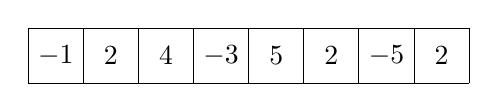
\begin{tikzpicture}[scale=0.7]
        \draw (0,0) grid (8,1);

        \node at (0.5,0.5) {$-1$};
        \node at (1.5,0.5) {$2$};
        \node at (2.5,0.5) {$4$};
        \node at (3.5,0.5) {$-3$};
        \node at (4.5,0.5) {$5$};
        \node at (5.5,0.5) {$2$};
        \node at (6.5,0.5) {$-5$};
        \node at (7.5,0.5) {$2$};
    \end{tikzpicture}
\end{center}
\begin{samepage}
    el siguiente subarreglo produce la suma máxima $10$:
    \begin{center}
        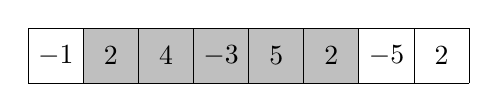
\begin{tikzpicture}[scale=0.7]
            \fill[color=lightgray] (1,0) rectangle (6,1);
            \draw (0,0) grid (8,1);

            \node at (0.5,0.5) {$-1$};
            \node at (1.5,0.5) {$2$};
            \node at (2.5,0.5) {$4$};
            \node at (3.5,0.5) {$-3$};
            \node at (4.5,0.5) {$5$};
            \node at (5.5,0.5) {$2$};
            \node at (6.5,0.5) {$-5$};
            \node at (7.5,0.5) {$2$};
        \end{tikzpicture}
    \end{center}
\end{samepage}

Asumimos que se permite un subarreglo vacío,
así que la suma máxima en subarreglo es siempre al menos $0$.

\subsubsection{Algoritmo 1}

Una forma sencilla de resolver el problema
es recorrer todos los subarreglos posibles,
calcular la suma de valores en cada subarreglo y mantener
la suma máxima.
El siguiente código implementa este algoritmo:

\begin{lstlisting}
int mejor = 0;
for (int a = 0; a < n; a++) {
    for (int b = a; b < n; b++) {
        int suma = 0;
        for (int k = a; k <= b; k++)
            suma += arreglo[k];
        mejor = max(mejor, suma);
    }
}
cout << mejor << "\n";
\end{lstlisting}

Las variables \texttt{a} y \texttt{b} fijan el primer y
último índice del subarreglo,
y la suma de valores se calcula en la variable \texttt{suma}.
La variable \texttt{mejor} contiene la suma máxima encontrada durante la búsqueda.

La complejidad temporal del algoritmo es $O(n^3)$,
porque consiste en tres bucles anidados
que recorren la entrada.

\subsubsection{Algoritmo 2}

Es fácil hacer el Algoritmo 1 más eficiente
eliminando un bucle de él.
Esto es posible calculando la suma al mismo
tiempo que se mueve el extremo derecho del subarreglo.
El resultado es el siguiente código:

\begin{lstlisting}
int mejor = 0;
for (int a = 0; a < n; a++) {
    int suma = 0;
    for (int b = a; b < n; b++) {
        suma += arreglo[b];
        mejor = max(mejor,suma);
    }
}
cout << mejor << "\n";
\end{lstlisting}
Después de este cambio, la complejidad en tiempo es $O(n^2)$.

\subsubsection{Algoritmo 3}

\index{algoritmo de!Kadane}

Sorprendentemente, es posible resolver el problema
en tiempo $O(n)$,\footnote{En \cite{ben86} este algoritmo de tiempo lineal
    se atribuye a J. B. Kadane, y el algoritmo a veces se
    llama \key{algoritmo de Kadane}.}, lo que significa
que solo se necesita un bucle.
La idea es calcular, para cada posición del arreglo,
la suma máxima de un subarreglo que termina en esa posición.
Después de esto, la respuesta al problema es el
máximo de esas sumas.

Consideremos el subproblema de encontrar el subarreglo de suma máxima
que termina en la posición $k$.
Hay dos posibilidades:
\begin{enumerate}
    \item El subarreglo solo contiene el elemento en la posición $k$.
    \item El subarreglo consta de un subarreglo que termina
          en la posición $k-1$, seguido del elemento en la posición $k$.
\end{enumerate}

En el último caso, dado que queremos
encontrar un subarreglo con suma máxima,
el subarreglo que termina en la posición $k-1$
también debe tener la suma máxima.
Por lo tanto, podemos resolver el problema de manera eficiente
calculando la suma de subarreglos máxima
para cada posición final de izquierda a derecha.

El siguiente código implementa el algoritmo:
\begin{lstlisting}
int mejor = 0, suma = 0;
for (int k = 0; k < n; k++) {
    suma = max(arreglo[k], suma + arreglo[k]);
    mejor = max(mejor, suma);
}
cout << best << "\n";
\end{lstlisting}

El algoritmo solo contiene un bucle
que recorre la entrada,
por lo que su complejidad temporal es $O(n)$.
Esta también es la mejor complejidad posible,
porque cualquier algoritmo para el problema
tiene que examinar todos los elementos del arreglo al menos una vez.

\subsubsection{Comparación de eficiencia}

Es interesante estudiar qué tan eficientes
son los algoritmos en la práctica.
La siguiente tabla muestra los tiempos de ejecución
de los algoritmos anteriores para diferentes
valores de $n$ en una computadora moderna.

En cada prueba, la entrada se generó al azar.
El tiempo necesario para leer la entrada no fue
medido.

\begin{center}
    \begin{tabular}{rrrr}
        tamaño del arreglo $n$ & Algoritmo 1 & Algoritmo 2 & Algoritmo 3 \\
        \hline
        $10^2$                 & $0,0$ s     & $0,0$ s     & $0,0$ s     \\
        $10^3$                 & $0,1$ s     & $0,0$ s     & $0,0$ s     \\
        $10^4$                 & > $10,0$ s  & $0,1$ s     & $0,0$ s     \\
        $10^5$                 & > $10,0$ s  & $5,3$ s     & $0,0$ s     \\
        $10^6$                 & > $10,0$ s  & > $10,0$ s  & $0,0$ s     \\
        $10^7$                 & > $10,0$ s  & > $10,0$ s  & $0,0$ s     \\
    \end{tabular}
\end{center}

La comparación muestra que todos los algoritmos
son eficientes cuando el tamaño de la entrada es pequeño,
pero las entradas más grandes resaltan diferencias notables
en los tiempos de ejecución de los algoritmos.
El Algoritmo 1 se vuelve lento
cuando $n=10^4$, y el Algoritmo 2
se vuelve lento cuando $n=10^5$.
Solo el Algoritmo 3 es capaz de procesar
incluso las entradas más grandes al instante.

\chapter{Ordenamiento}

\index{ordenamiento}

\key{Ordenamiento}
es un problema fundamental en el diseño de algoritmos.
Muchos algoritmos eficientes
usan el ordenamiento como una subrutina,
ya que a menudo es más fácil procesar
datos si los elementos están en orden.

Por ejemplo, el problema "¿un arreglo contiene
dos elementos iguales?" es fácil de resolver usando ordenamiento.
Si el arreglo contiene dos elementos iguales,
estarán uno al lado del otro después de ordenar,
así que es fácil encontrarlos.
Además, el problema "¿cuál es el elemento más frecuente
en un arreglo?" se puede resolver de manera similar.

Hay muchos algoritmos para ordenar, y también son
buenos ejemplos de cómo aplicar
diferentes técnicas de diseño de algoritmos.
Los algoritmos generales de ordenamiento eficientes
funcionan en tiempo $O(n \log n)$,
y muchos algoritmos que utilizan ordenamiento
como una subrutina también
tienen esta complejidad de tiempo.

\section{Teoría del ordenamiento}

El problema básico en el ordenamiento es el siguiente:
\begin{framed}
\noindent
Dado un arreglo que contiene $n$ elementos,
tu tarea es ordenar los elementos
en orden ascendente.
\end{framed}
\noindent
Por ejemplo, el arreglo
\begin{center}
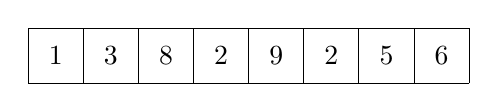
\begin{tikzpicture}[scale=0.7]
\draw (0,0) grid (8,1);
\node at (0.5,0.5) {$1$};
\node at (1.5,0.5) {$3$};
\node at (2.5,0.5) {$8$};
\node at (3.5,0.5) {$2$};
\node at (4.5,0.5) {$9$};
\node at (5.5,0.5) {$2$};
\node at (6.5,0.5) {$5$};
\node at (7.5,0.5) {$6$};
\end{tikzpicture}
\end{center}
será como sigue después de ordenar:
\begin{center}
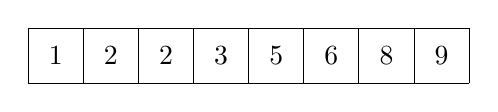
\begin{tikzpicture}[scale=0.7]
\draw (0,0) grid (8,1);
\node at (0.5,0.5) {$1$};
\node at (1.5,0.5) {$2$};
\node at (2.5,0.5) {$2$};
\node at (3.5,0.5) {$3$};
\node at (4.5,0.5) {$5$};
\node at (5.5,0.5) {$6$};
\node at (6.5,0.5) {$8$};
\node at (7.5,0.5) {$9$};
\end{tikzpicture}
\end{center}

\subsubsection{Algoritmos $O(n^2)$}

\index{ordenamiento burbuja}

Los algoritmos simples para ordenar un arreglo
funcionan en tiempo $O(n^2)$.
Estos algoritmos son cortos y generalmente
consisten en dos bucles anidados.
Un famoso algoritmo de ordenamiento en tiempo $O(n^2)$
es el \key{ordenamiento burbuja}, donde los elementos
''burbujean'' en el arreglo según sus valores.

Bubble sort consta de $n$ rondas.
En cada ronda, el algoritmo itera a través
de los elementos del arreglo.
Siempre que se encuentran dos elementos consecutivos
que no están en el orden correcto,
el algoritmo los intercambia.
El algoritmo se puede implementar de la siguiente manera:
\begin{lstlisting}
for (int i = 0; i < n; i++) {
    for (int j = 0; j < n-1; j++) {
        if (array[j] > array[j+1]) {
            swap(array[j],array[j+1]);
        }
    }
}
\end{lstlisting}

Después de la primera ronda del algoritmo,
el elemento más grande estará en la posición correcta,
y en general, después de $k$ rondas, los $k$ elementos más grandes
estarán en las posiciones correctas.
Por lo tanto, después de $n$ rondas, todo el arreglo
estará ordenado.

Por ejemplo, en el arreglo

\begin{center}
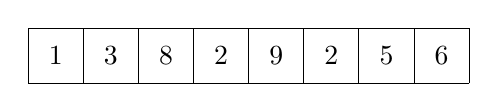
\begin{tikzpicture}[scale=0.7]
\draw (0,0) grid (8,1);

\node at (0.5,0.5) {$1$};
\node at (1.5,0.5) {$3$};
\node at (2.5,0.5) {$8$};
\node at (3.5,0.5) {$2$};
\node at (4.5,0.5) {$9$};
\node at (5.5,0.5) {$2$};
\node at (6.5,0.5) {$5$};
\node at (7.5,0.5) {$6$};
\end{tikzpicture}
\end{center}

\noindent
la primera ronda de bubble sort intercambia elementos
como sigue:

\begin{center}
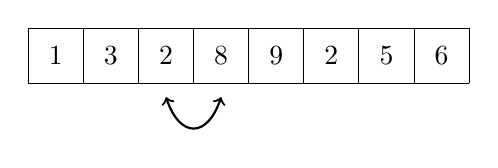
\begin{tikzpicture}[scale=0.7]
\draw (0,0) grid (8,1);
\node at (0.5,0.5) {$1$};
\node at (1.5,0.5) {$3$};
\node at (2.5,0.5) {$2$};
\node at (3.5,0.5) {$8$};
\node at (4.5,0.5) {$9$};
\node at (5.5,0.5) {$2$};
\node at (6.5,0.5) {$5$};
\node at (7.5,0.5) {$6$};

\draw[thick,<->] (3.5,-0.25) .. controls (3.25,-1.00) and (2.75,-1.00) .. (2.5,-0.25);
\end{tikzpicture}
\end{center}

\begin{center}
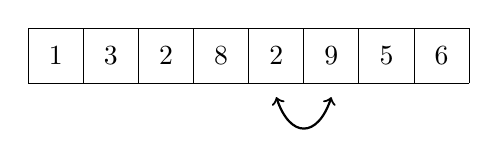
\begin{tikzpicture}[scale=0.7]
\draw (0,0) grid (8,1);
\node at (0.5,0.5) {$1$};
\node at (1.5,0.5) {$3$};
\node at (2.5,0.5) {$2$};
\node at (3.5,0.5) {$8$};
\node at (4.5,0.5) {$2$};
\node at (5.5,0.5) {$9$};
\node at (6.5,0.5) {$5$};
\node at (7.5,0.5) {$6$};

\draw[thick,<->] (5.5,-0.25) .. controls (5.25,-1.00) and (4.75,-1.00) .. (4.5,-0.25);
\end{tikzpicture}
\end{center}

\begin{center}
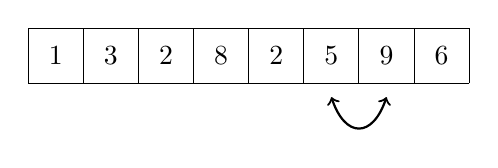
\begin{tikzpicture}[scale=0.7]
\draw (0,0) grid (8,1);
\node at (0.5,0.5) {$1$};
\node at (1.5,0.5) {$3$};
\node at (2.5,0.5) {$2$};
\node at (3.5,0.5) {$8$};
\node at (4.5,0.5) {$2$};
\node at (5.5,0.5) {$5$};
\node at (6.5,0.5) {$9$};
\node at (7.5,0.5) {$6$};

\draw[thick,<->] (6.5,-0.25) .. controls (6.25,-1.00) and (5.75,-1.00) .. (5.5,-0.25);
\end{tikzpicture}
\end{center}

\begin{center}
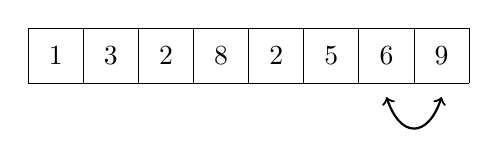
\begin{tikzpicture}[scale=0.7]
\draw (0,0) grid (8,1);
\node at (0.5,0.5) {$1$};
\node at (1.5,0.5) {$3$};
\node at (2.5,0.5) {$2$};
\node at (3.5,0.5) {$8$};
\node at (4.5,0.5) {$2$};
\node at (5.5,0.5) {$5$};
\node at (6.5,0.5) {$6$};
\node at (7.5,0.5) {$9$};

\draw[thick,<->] (7.5,-0.25) .. controls (7.25,-1.00) and (6.75,-1.00) .. (6.5,-0.25);
\end{tikzpicture}
\end{center}

\subsubsection{Inversiones}

\index{inversión}

Bubble sort es un ejemplo de un algoritmo de ordenamiento
que siempre intercambia elementos \emph{consecutivos}
en el arreglo.
Resulta que la complejidad temporal
de tal algoritmo es \emph{siempre}
al menos $O(n^2)$, porque en el peor caso,
se requieren $O(n^2)$ intercambios para ordenar el arreglo.

Un concepto útil al analizar algoritmos de ordenamiento
es una \key{inversión}:
un par de elementos del arreglo
$(\texttt{array}[a],\texttt{array}[b])$ tal que
$a<b$ y $\texttt{array}[a]>\texttt{array}[b]$,
es decir, los elementos están en el orden incorrecto.
Por ejemplo, el arreglo
\begin{center}
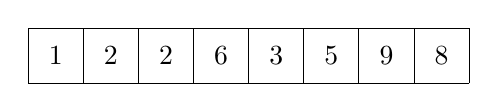
\begin{tikzpicture}[scale=0.7]
\draw (0,0) grid (8,1);
\node at (0.5,0.5) {$1$};
\node at (1.5,0.5) {$2$};
\node at (2.5,0.5) {$2$};
\node at (3.5,0.5) {$6$};
\node at (4.5,0.5) {$3$};
\node at (5.5,0.5) {$5$};
\node at (6.5,0.5) {$9$};
\node at (7.5,0.5) {$8$};
\end{tikzpicture}
\end{center}
tiene tres inversiones: $(6,3)$, $(6,5)$ y $(9,8)$.
El número de inversiones indica
cuánto trabajo se necesita para ordenar el arreglo.
Un arreglo está completamente ordenado cuando
no hay inversiones.
Por otro lado, si los elementos del arreglo
están en orden inverso,
el número de inversiones es el mayor posible:
\[1+2+\cdots+(n-1)=\frac{n(n-1)}{2} = O(n^2)\]

Intercambiar un par de elementos consecutivos que están
en el orden incorrecto elimina exactamente una inversión
del arreglo.
Por lo tanto, si un algoritmo de ordenamiento solo puede
intercambiar elementos consecutivos, cada intercambio elimina
como máximo una inversión, y la complejidad en tiempo
del algoritmo es al menos $O(n^2)$.

\subsubsection{$O(n \log n)$ algoritmos}

\index{ordenamiento por mezcla}

Es posible ordenar un arreglo de manera eficiente
en tiempo $O(n \log n)$ utilizando algoritmos
que no se limitan a intercambiar elementos consecutivos.
Un algoritmo de este tipo es el \key{ordenamiento por mezcla}\footnote{Según \cite{knu983},
el ordenamiento por mezcla fue inventado por J. von Neumann en 1945.},
que se basa en la recursión.

El ordenamiento por mezcla ordena un subarreglo \texttt{array}$[a \ldots b]$ de la siguiente manera:

\begin{enumerate}
\item Si $a=b$, no hacer nada, porque el subarreglo ya está ordenado.
\item Calcular la posición del elemento medio: $k=\lfloor (a+b)/2 \rfloor$.
\item Ordenar recursivamente el subarreglo \texttt{array}$[a \ldots k]$.
\item Ordenar recursivamente el subarreglo \texttt{array}$[k+1 \ldots b]$.
\item \emph{Mezclar} los subarreglos ordenados \texttt{array}$[a \ldots k]$ y
\texttt{array}$[k+1 \ldots b]$
en un subarreglo ordenado \texttt{array}$[a \ldots b]$.
\end{enumerate}

El ordenamiento por mezcla es un algoritmo eficiente, ya que
reduce a la mitad el tamaño del subarreglo en cada paso.
La recursión consta de $O(\log n)$ niveles,
y procesar cada nivel toma $O(n)$ tiempo.
Mezclar los subarreglos \texttt{array}$[a \ldots k]$ y \texttt{array}$[k+1 \ldots b]$
es posible en tiempo lineal, porque ya están ordenados.

Por ejemplo, considere ordenar el siguiente arreglo:
\begin{center}
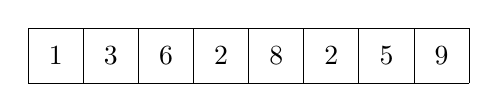
\begin{tikzpicture}[scale=0.7]
\draw (0,0) grid (8,1);
\node at (0.5,0.5) {$1$};
\node at (1.5,0.5) {$3$};
\node at (2.5,0.5) {$6$};
\node at (3.5,0.5) {$2$};
\node at (4.5,0.5) {$8$};
\node at (5.5,0.5) {$2$};
\node at (6.5,0.5) {$5$};
\node at (7.5,0.5) {$9$};
\end{tikzpicture}
\end{center}

El arreglo se dividirá en dos subarreglos
de la siguiente manera:
\begin{center}
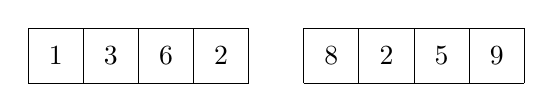
\begin{tikzpicture}[scale=0.7]
\draw (0,0) grid (4,1);
\draw (5,0) grid (9,1);

\node at (0.5,0.5) {$1$};
\node at (1.5,0.5) {$3$};
\node at (2.5,0.5) {$6$};
\node at (3.5,0.5) {$2$};

\node at (5.5,0.5) {$8$};
\node at (6.5,0.5) {$2$};
\node at (7.5,0.5) {$5$};
\node at (8.5,0.5) {$9$};
\end{tikzpicture}
\end{center}

Then, the subarrays will be sorted recursively
as follows:
\begin{center}
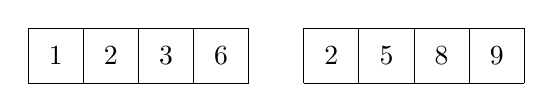
\begin{tikzpicture}[scale=0.7]
\draw (0,0) grid (4,1);
\draw (5,0) grid (9,1);

\node at (0.5,0.5) {$1$};
\node at (1.5,0.5) {$2$};
\node at (2.5,0.5) {$3$};
\node at (3.5,0.5) {$6$};

\node at (5.5,0.5) {$2$};
\node at (6.5,0.5) {$5$};
\node at (7.5,0.5) {$8$};
\node at (8.5,0.5) {$9$};
\end{tikzpicture}
\end{center}

Finally, the algorithm merges the sorted
subarrays and creates the final sorted array:
\begin{center}
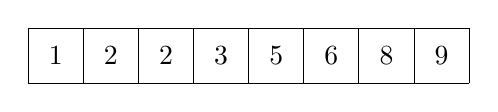
\begin{tikzpicture}[scale=0.7]
\draw (0,0) grid (8,1);
\node at (0.5,0.5) {$1$};
\node at (1.5,0.5) {$2$};
\node at (2.5,0.5) {$2$};
\node at (3.5,0.5) {$3$};
\node at (4.5,0.5) {$5$};
\node at (5.5,0.5) {$6$};
\node at (6.5,0.5) {$8$};
\node at (7.5,0.5) {$9$};
\end{tikzpicture}
\end{center}

\subsubsection{Sorting lower bound}

Is it possible to sort an array faster
than in $O(n \log n)$ time?
It turns out that this is \emph{not} possible
when we restrict ourselves to sorting algorithms
that are based on comparing array elements.

The lower bound for the time complexity
can be proved by considering sorting
as a process where each comparison of two elements
gives more information about the contents of the array.
The process creates the following tree:

\begin{center}
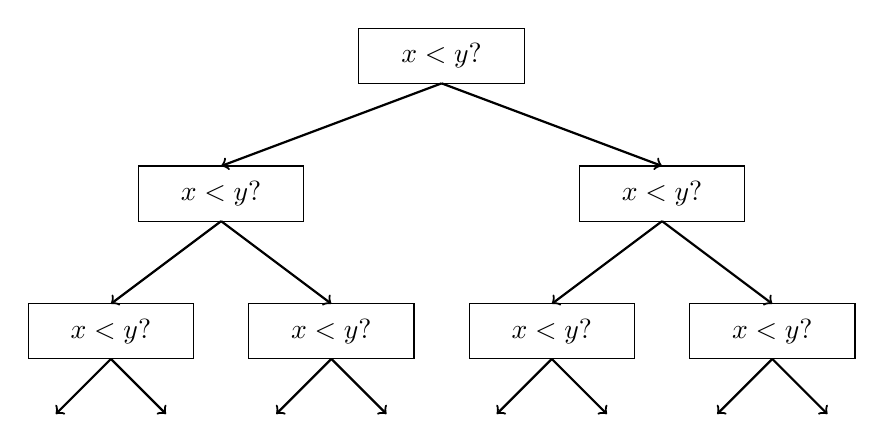
\begin{tikzpicture}[scale=0.7]
\draw (0,0) rectangle (3,1);
\node at (1.5,0.5) {$x < y?$};

\draw[thick,->] (1.5,0) -- (-2.5,-1.5);
\draw[thick,->] (1.5,0) -- (5.5,-1.5);

\draw (-4,-2.5) rectangle (-1,-1.5);
\draw (4,-2.5) rectangle (7,-1.5);
\node at (-2.5,-2) {$x < y?$};
\node at (5.5,-2) {$x < y?$};

\draw[thick,->] (-2.5,-2.5) -- (-4.5,-4);
\draw[thick,->] (-2.5,-2.5) -- (-0.5,-4);
\draw[thick,->] (5.5,-2.5) -- (3.5,-4);
\draw[thick,->] (5.5,-2.5) -- (7.5,-4);

\draw (-6,-5) rectangle (-3,-4);
\draw (-2,-5) rectangle (1,-4);
\draw (2,-5) rectangle (5,-4);
\draw (6,-5) rectangle (9,-4);
\node at (-4.5,-4.5) {$x < y?$};
\node at (-0.5,-4.5) {$x < y?$};
\node at (3.5,-4.5) {$x < y?$};
\node at (7.5,-4.5) {$x < y?$};

\draw[thick,->] (-4.5,-5) -- (-5.5,-6);
\draw[thick,->] (-4.5,-5) -- (-3.5,-6);
\draw[thick,->] (-0.5,-5) -- (0.5,-6);
\draw[thick,->] (-0.5,-5) -- (-1.5,-6);
\draw[thick,->] (3.5,-5) -- (2.5,-6);
\draw[thick,->] (3.5,-5) -- (4.5,-6);
\draw[thick,->] (7.5,-5) -- (6.5,-6);
\draw[thick,->] (7.5,-5) -- (8.5,-6);
\end{tikzpicture}
\end{center}

Here ''$x<y?$'' means that some elements
$x$ and $y$ are compared.
If $x<y$, the process continues to the left,
and otherwise to the right.
The results of the process are the possible
ways to sort the array, a total of $n!$ ways.
For this reason, the height of the tree
must be at least
\[ \log_2(n!) = \log_2(1)+\log_2(2)+\cdots+\log_2(n).\]
We get a lower bound for this sum
by choosing the last $n/2$ elements and
changing the value of each element to $\log_2(n/2)$.
This yields an estimate
\[ \log_2(n!) \ge (n/2) \cdot \log_2(n/2),\]
so the height of the tree and the minimum
possible number of steps in a sorting
algorithm in the worst case
is at least $n \log n$.

\subsubsection{Counting sort}

\index{counting sort}

The lower bound $n \log n$ does not apply to
algorithms that do not compare array elements
but use some other information.
An example of such an algorithm is
\key{counting sort} that sorts an array in
$O(n)$ time assuming that every element in the array
is an integer between $0 \ldots c$ and $c=O(n)$.

The algorithm creates a \emph{bookkeeping} array,
whose indices are elements of the original array.
The algorithm iterates through the original array
and calculates how many times each element
appears in the array.
\newpage

For example, the array
\begin{center}
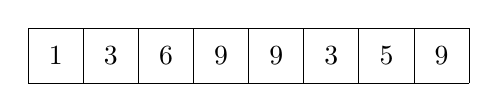
\begin{tikzpicture}[scale=0.7]
\draw (0,0) grid (8,1);
\node at (0.5,0.5) {$1$};
\node at (1.5,0.5) {$3$};
\node at (2.5,0.5) {$6$};
\node at (3.5,0.5) {$9$};
\node at (4.5,0.5) {$9$};
\node at (5.5,0.5) {$3$};
\node at (6.5,0.5) {$5$};
\node at (7.5,0.5) {$9$};
\end{tikzpicture}
\end{center}
corresponds to the following bookkeeping array:
\begin{center}
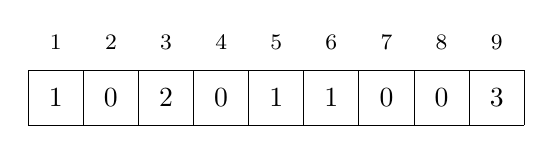
\begin{tikzpicture}[scale=0.7]
\draw (0,0) grid (9,1);
\node at (0.5,0.5) {$1$};
\node at (1.5,0.5) {$0$};
\node at (2.5,0.5) {$2$};
\node at (3.5,0.5) {$0$};
\node at (4.5,0.5) {$1$};
\node at (5.5,0.5) {$1$};
\node at (6.5,0.5) {$0$};
\node at (7.5,0.5) {$0$};
\node at (8.5,0.5) {$3$};

\footnotesize

\node at (0.5,1.5) {$1$};
\node at (1.5,1.5) {$2$};
\node at (2.5,1.5) {$3$};
\node at (3.5,1.5) {$4$};
\node at (4.5,1.5) {$5$};
\node at (5.5,1.5) {$6$};
\node at (6.5,1.5) {$7$};
\node at (7.5,1.5) {$8$};
\node at (8.5,1.5) {$9$};
\end{tikzpicture}
\end{center}

For example, the value at position 3
in the bookkeeping array is 2,
because the element 3 appears 2 times
in the original array.

Construction of the bookkeeping array
takes $O(n)$ time. After this, the sorted array
can be created in $O(n)$ time because
the number of occurrences of each element can be retrieved
from the bookkeeping array.
Thus, the total time complexity of counting
sort is $O(n)$.

Counting sort is a very efficient algorithm
but it can only be used when the constant $c$
is small enough, so that the array elements can
be used as indices in the bookkeeping array.

\section{Sorting in C++}

\index{sort@\texttt{sort}}

It is almost never a good idea to use
a home-made sorting algorithm
in a contest, because there are good
implementations available in programming languages.
For example, the C++ standard library contains
the function \texttt{sort} that can be easily used for
sorting arrays and other data structures.

There are many benefits in using a library function.
First, it saves time because there is no need to
implement the function.
Second, the library implementation is
certainly correct and efficient: it is not probable
that a home-made sorting function would be better.

In this section we will see how to use the
C++ \texttt{sort} function.
The following code sorts
a vector in increasing order:
\begin{lstlisting}
vector<int> v = {4,2,5,3,5,8,3};
sort(v.begin(),v.end());
\end{lstlisting}
After the sorting, the contents of the
vector will be
$[2,3,3,4,5,5,8]$.
The default sorting order is increasing,
but a reverse order is possible as follows:
\begin{lstlisting}
sort(v.rbegin(),v.rend());
\end{lstlisting}
An ordinary array can be sorted as follows:
\begin{lstlisting}
int n = 7; // array size
int a[] = {4,2,5,3,5,8,3};
sort(a,a+n);
\end{lstlisting}
\newpage
The following code sorts the string \texttt{s}:
\begin{lstlisting}
string s = "monkey";
sort(s.begin(), s.end());
\end{lstlisting}
Sorting a string means that the characters
of the string are sorted.
For example, the string ''monkey'' becomes ''ekmnoy''.

\subsubsection{Comparison operators}

\index{comparison operator}

The function \texttt{sort} requires that
a \key{comparison operator} is defined for the data type
of the elements to be sorted.
When sorting, this operator will be used
whenever it is necessary to find out the order of two elements.

Most C++ data types have a built-in comparison operator,
and elements of those types can be sorted automatically.
For example, numbers are sorted according to their values
and strings are sorted in alphabetical order.

\index{pair@\texttt{pair}}

Pairs (\texttt{pair}) are sorted primarily according to their
first elements (\texttt{first}).
However, if the first elements of two pairs are equal,
they are sorted according to their second elements (\texttt{second}):
\begin{lstlisting}
vector<pair<int,int>> v;
v.push_back({1,5});
v.push_back({2,3});
v.push_back({1,2});
sort(v.begin(), v.end());
\end{lstlisting}
After this, the order of the pairs is
$(1,2)$, $(1,5)$ and $(2,3)$.

\index{tuple@\texttt{tuple}}

In a similar way, tuples (\texttt{tuple})
are sorted primarily by the first element,
secondarily by the second element, etc.\footnote{Note that in some older compilers,
the function \texttt{make\_tuple} has to be used to create a tuple instead of
braces (for example, \texttt{make\_tuple(2,1,4)} instead of \texttt{\{2,1,4\}}).}:
\begin{lstlisting}
vector<tuple<int,int,int>> v;
v.push_back({2,1,4});
v.push_back({1,5,3});
v.push_back({2,1,3});
sort(v.begin(), v.end());
\end{lstlisting}
After this, the order of the tuples is
$(1,5,3)$, $(2,1,3)$ and $(2,1,4)$.

\subsubsection{User-defined structs}

User-defined structs do not have a comparison
operator automatically.
The operator should be defined inside
the struct as a function
\texttt{operator<},
whose parameter is another element of the same type.
The operator should return \texttt{true}
if the element is smaller than the parameter,
and \texttt{false} otherwise.

For example, the following struct \texttt{P}
contains the x and y coordinates of a point.
The comparison operator is defined so that
the points are sorted primarily by the x coordinate
and secondarily by the y coordinate.

\begin{lstlisting}
struct P {
    int x, y;
    bool operator<(const P &p) {
        if (x != p.x) return x < p.x;
        else return y < p.y;
    }
};
\end{lstlisting}

\subsubsection{Comparison functions}

\index{comparison function}

It is also possible to give an external
\key{comparison function} to the \texttt{sort} function
as a callback function.
For example, the following comparison function \texttt{comp}
sorts strings primarily by length and secondarily
by alphabetical order:

\begin{lstlisting}
bool comp(string a, string b) {
    if (a.size() != b.size()) return a.size() < b.size();
    return a < b;
}
\end{lstlisting}
Now a vector of strings can be sorted as follows:
\begin{lstlisting}
sort(v.begin(), v.end(), comp);
\end{lstlisting}

\section{Binary search}

\index{binary search}

A general method for searching for an element
in an array is to use a \texttt{for} loop
that iterates through the elements of the array.
For example, the following code searches for
an element $x$ in an array:

\begin{lstlisting}
for (int i = 0; i < n; i++) {
    if (array[i] == x) {
        // x found at index i
    }
}
\end{lstlisting}

The time complexity of this approach is $O(n)$,
because in the worst case, it is necessary to check
all elements of the array.
If the order of the elements is arbitrary,
this is also the best possible approach, because
there is no additional information available where
in the array we should search for the element $x$.

However, if the array is \emph{sorted},
the situation is different.
In this case it is possible to perform the
search much faster, because the order of the
elements in the array guides the search.
The following \key{binary search} algorithm
efficiently searches for an element in a sorted array
in $O(\log n)$ time.

\subsubsection{Method 1}

The usual way to implement binary search
resembles looking for a word in a dictionary.
The search maintains an active region in the array,
which initially contains all array elements.
Then, a number of steps is performed,
each of which halves the size of the region.

At each step, the search checks the middle element
of the active region.
If the middle element is the target element,
the search terminates.
Otherwise, the search recursively continues
to the left or right half of the region,
depending on the value of the middle element.

The above idea can be implemented as follows:
\begin{lstlisting}
int a = 0, b = n-1;
while (a <= b) {
    int k = (a+b)/2;
    if (array[k] == x) {
        // x found at index k
    }
    if (array[k] > x) b = k-1;
    else a = k+1;
}
\end{lstlisting}

In this implementation, the active region is $a \ldots b$,
and initially the region is $0 \ldots n-1$.
The algorithm halves the size of the region at each step,
so the time complexity is $O(\log n)$.

\subsubsection{Method 2}

An alternative method to implement binary search
is based on an efficient way to iterate through
the elements of the array.
The idea is to make jumps and slow the speed
when we get closer to the target element.

The search goes through the array from left to
right, and the initial jump length is $n/2$.
At each step, the jump length will be halved:
first $n/4$, then $n/8$, $n/16$, etc., until
finally the length is 1.
After the jumps, either the target element has
been found or we know that it does not appear in the array.

The following code implements the above idea:
\begin{lstlisting}
int k = 0;
for (int b = n/2; b >= 1; b /= 2) {
    while (k+b < n && array[k+b] <= x) k += b;
}
if (array[k] == x) {
    // x found at index k
}
\end{lstlisting}

During the search, the variable $b$
contains the current jump length.
The time complexity of the algorithm is $O(\log n)$,
because the code in the \texttt{while} loop
is performed at most twice for each jump length.

\subsubsection{C++ functions}

The C++ standard library contains the following functions
that are based on binary search and work in logarithmic time:

\begin{itemize}
\item \texttt{lower\_bound} returns a pointer to the
first array element whose value is at least $x$.
\item \texttt{upper\_bound} returns a pointer to the
first array element whose value is larger than $x$.
\item \texttt{equal\_range} returns both above pointers.
\end{itemize}

The functions assume that the array is sorted.
If there is no such element, the pointer points to
the element after the last array element.
For example, the following code finds out whether
an array contains an element with value $x$:

\begin{lstlisting}
auto k = lower_bound(array,array+n,x)-array;
if (k < n && array[k] == x) {
    // x found at index k
}
\end{lstlisting}

Then, the following code counts the number of elements
whose value is $x$:

\begin{lstlisting}
auto a = lower_bound(array, array+n, x);
auto b = upper_bound(array, array+n, x);
cout << b-a << "\n";
\end{lstlisting}

Using \texttt{equal\_range}, the code becomes shorter:

\begin{lstlisting}
auto r = equal_range(array, array+n, x);
cout << r.second-r.first << "\n";
\end{lstlisting}

\subsubsection{Finding the smallest solution}

An important use for binary search is
to find the position where the value of a \emph{function} changes.
Suppose that we wish to find the smallest value $k$
that is a valid solution for a problem.
We are given a function $\texttt{ok}(x)$
that returns \texttt{true} if $x$ is a valid solution
and \texttt{false} otherwise.
In addition, we know that $\texttt{ok}(x)$ is \texttt{false}
when $x<k$ and \texttt{true} when $x \ge k$.
The situation looks as follows:

\begin{center}
\begin{tabular}{r|rrrrrrrr}
$x$ & 0 & 1 & $\cdots$ & $k-1$ & $k$ & $k+1$ & $\cdots$ \\
\hline
$\texttt{ok}(x)$ & \texttt{false} & \texttt{false}
& $\cdots$ & \texttt{false} & \texttt{true} & \texttt{true} & $\cdots$ \\
\end{tabular}
\end{center}

\noindent
Now, the value of $k$ can be found using binary search:

\begin{lstlisting}
int x = -1;
for (int b = z; b >= 1; b /= 2) {
    while (!ok(x+b)) x += b;
}
int k = x+1;
\end{lstlisting}

The search finds the largest value of $x$ for which
$\texttt{ok}(x)$ is \texttt{false}.
Thus, the next value $k=x+1$
is the smallest possible value for which
$\texttt{ok}(k)$ is \texttt{true}.
The initial jump length $z$ has to be
large enough, for example some value
for which we know beforehand that $\texttt{ok}(z)$ is \texttt{true}.

The algorithm calls the function \texttt{ok}
$O(\log z)$ times, so the total time complexity
depends on the function \texttt{ok}.
For example, if the function works in $O(n)$ time,
the total time complexity is $O(n \log z)$.

\subsubsection{Finding the maximum value}

Binary search can also be used to find
the maximum value for a function that is
first increasing and then decreasing.
Our task is to find a position $k$ such that

\begin{itemize}
\item
$f(x)<f(x+1)$ when $x<k$, and
\item
$f(x)>f(x+1)$ when $x \ge k$.
\end{itemize}

The idea is to use binary search
for finding the largest value of $x$
for which $f(x)<f(x+1)$.
This implies that $k=x+1$
because $f(x+1)>f(x+2)$.
The following code implements the search: 

\begin{lstlisting}
int x = -1;
for (int b = z; b >= 1; b /= 2) {
    while (f(x+b) < f(x+b+1)) x += b;
}
int k = x+1;
\end{lstlisting}

Note that unlike in the ordinary binary search,
here it is not allowed that consecutive values
of the function are equal.
In this case it would not be possible to know
how to continue the search.

\chapter{Estructuras de datos}

\index{estructura de datos}

Una \key{estructura de datos} es una forma de almacenar
datos en la memoria de una computadora.
Es importante elegir una estructura de datos adecuada
para un problema,
ya que cada estructura de datos tiene sus propias
ventajas y desventajas.
La pregunta crucial es: ¿qué operaciones
son eficientes en la estructura de datos elegida?

Este capítulo presenta las estructuras de datos más importantes
de la biblioteca estándar de C++.
Es una buena idea utilizar la biblioteca estándar
siempre que sea posible,
porque ahorrará mucho tiempo.
Más adelante en el libro, aprenderemos sobre estructuras de datos más sofisticadas
que no están disponibles
en la biblioteca estándar.

\section{Arreglos dinámicos}

\index{arreglo dinámico}
\index{vector}

Un \key{arreglo dinámico} es un arreglo cuyo
tamaño puede cambiar durante la ejecución
del programa.
El arreglo dinámico más popular en C++ es
la estructura \texttt{vector},
que se puede utilizar casi como un arreglo ordinario.

El siguiente código crea un vector vacío y
añade tres elementos a él:

\begin{lstlisting}
vector<int> v;
v.push_back(3); // [3]
v.push_back(2); // [3,2]
v.push_back(5); // [3,2,5]
\end{lstlisting}

Después de esto, los elementos se pueden acceder como en un arreglo ordinario:

\begin{lstlisting}
cout << v[0] << "\n"; // 3
cout << v[1] << "\n"; // 2
cout << v[2] << "\n"; // 5
\end{lstlisting}

La función \texttt{size} devuelve el número de elementos en el vector.
El siguiente código itera a través
del vector e imprime todos los elementos en él:

\begin{lstlisting}
for (int i = 0; i < v.size(); i++) {
    cout << v[i] << "\n";
}
\end{lstlisting}

\begin{samepage}
Una forma más corta de iterar a través de un vector es la siguiente:

\begin{lstlisting}
for (auto x : v) {
    cout << x << "\n";
}
\end{lstlisting}
\end{samepage}

La función \texttt{back} devuelve el último elemento
en el vector, y
la función \texttt{pop\_back} elimina el último elemento:

\begin{lstlisting}
vector<int> v;
v.push_back(5);
v.push_back(2);
cout << v.back() << "\n"; // 2
v.pop_back();
cout << v.back() << "\n"; // 5
\end{lstlisting}

El siguiente código crea un vector con cinco elementos:

\begin{lstlisting}
vector<int> v = {2,4,2,5,1};
\end{lstlisting}

Otra forma de crear un vector es proporcionar el número
de elementos y el valor inicial para cada elemento:

\begin{lstlisting}
// tamaño 10, valor inicial 0
vector<int> v(10);
\end{lstlisting}
\begin{lstlisting}
// tamaño 10, valor inicial 5
vector<int> v(10, 5);
\end{lstlisting}

La implementación interna de un vector
utiliza un arreglo ordinario.
Si el tamaño del vector aumenta y
el arreglo se vuelve demasiado pequeño,
se asigna un nuevo arreglo y todos los
elementos se mueven al nuevo arreglo.
Sin embargo, esto no sucede a menudo y la
complejidad de tiempo promedio de
\texttt{push\_back} es $O(1)$.

\index{string}

La estructura \texttt{string} también es un arreglo dinámico que
puede ser utilizado casi como un vector.
Además, existe una sintaxis especial para las cadenas
que no está disponible en otras estructuras de datos.
Las cadenas se pueden combinar utilizando el símbolo \texttt{+}.
La función $\texttt{substr}(k,x)$ devuelve la subcadena
que comienza en la posición $k$ y tiene una longitud de $x$,
y la función $\texttt{find}(\texttt{t})$ encuentra la posición
de la primera aparición de una subcadena \texttt{t}.

El siguiente código presenta algunas operaciones de cadenas:

\begin{lstlisting}
string a = "hatti";
string b = a+a;
cout << b << "\n"; // hattihatti
b[5] = 'v';
cout << b << "\n"; // hattivatti
string c = b.substr(3,4);
cout << c << "\n"; // tiva
\end{lstlisting}

\section{Estructuras de conjuntos}

\index{set}

Un \key{conjunto} es una estructura de datos que
mantiene una colección de elementos.
Las operaciones básicas de los conjuntos son la inserción
de elementos, búsqueda y eliminación.

La biblioteca estándar de C++ contiene dos implementaciones
de conjuntos:
La estructura \texttt{set} se basa en un árbol binario equilibrado
y sus operaciones funcionan en tiempo $O(\log n)$.
La estructura \texttt{unordered\_set} utiliza hashing
y sus operaciones funcionan en tiempo promedio de $O(1)$.

La elección de qué implementación de conjunto utilizar
a menudo es una cuestión de preferencia.
El beneficio de la estructura \texttt{set} es que mantiene
el orden de los elementos y proporciona funciones que
no están disponibles en \texttt{unordered\_set}.
Por otro lado, \texttt{unordered\_set}
puede ser más eficiente.

El siguiente código crea un conjunto
que contiene enteros,
y muestra algunas de las operaciones.
La función \texttt{insert} agrega un elemento al conjunto,
la función \texttt{count} devuelve el número de ocurrencias
de un elemento en el conjunto,
y la función \texttt{erase} elimina un elemento del conjunto.

\begin{lstlisting}
set<int> s;
s.insert(3);
s.insert(2);
s.insert(5);
cout << s.count(3) << "\n"; // 1
cout << s.count(4) << "\n"; // 0
s.erase(3);
s.insert(4);
cout << s.count(3) << "\n"; // 0
cout << s.count(4) << "\n"; // 1
\end{lstlisting}

Un conjunto se puede utilizar principalmente como un vector,
pero no es posible acceder
a los elementos utilizando la notación \texttt{[]}.
El siguiente código crea un conjunto,
imprime el número de elementos en él y luego
itera a través de todos los elementos:
\begin{lstlisting}
set<int> s = {2,5,6,8};
cout << s.size() << "\n"; // 4
for (auto x : s) {
    cout << x << "\n";
}
\end{lstlisting}

Una propiedad importante de los conjuntos es
que todos sus elementos son \emph{distintos}.
Por lo tanto, la función \texttt{count} siempre devuelve
0 (el elemento no está en el conjunto)
o 1 (el elemento está en el conjunto),
y la función \texttt{insert} nunca agrega
un elemento al conjunto si ya está
presente.
El siguiente código ilustra esto:

\begin{lstlisting}
set<int> s;
s.insert(5);
s.insert(5);
s.insert(5);
cout << s.count(5) << "\n"; // 1
\end{lstlisting}

C++ también contiene las estructuras
\texttt{multiset} y \texttt{unordered\_multiset}
que funcionan de manera similar a \texttt{set}
y \texttt{unordered\_set}
pero pueden contener múltiples instancias de un elemento.
Por ejemplo, en el siguiente código, se agregan las tres instancias
del número 5 a un multiset:

\begin{lstlisting}
multiset<int> s;
s.insert(5);
s.insert(5);
s.insert(5);
cout << s.count(5) << "\n"; // 3
\end{lstlisting}
La función \texttt{erase} elimina
todas las instancias de un elemento
de un multiset:
\begin{lstlisting}
s.erase(5);
cout << s.count(5) << "\n"; // 0
\end{lstlisting}
A menudo, solo se debe eliminar una instancia,
lo cual se puede hacer de la siguiente manera:
\begin{lstlisting}
s.erase(s.find(5));
cout << s.count(5) << "\n"; // 2
\end{lstlisting}

\section{Map structures}

\index{map}

A \key{map} is a generalized array
that consists of key-value-pairs.
While the keys in an ordinary array are always
the consecutive integers $0,1,\ldots,n-1$,
where $n$ is the size of the array,
the keys in a map can be of any data type and
they do not have to be consecutive values.

The C++ standard library contains two map
implementations that correspond to the set
implementations: the structure
\texttt{map} is based on a balanced
binary tree and accessing elements
takes $O(\log n)$ time,
while the structure
\texttt{unordered\_map} uses hashing
and accessing elements takes $O(1)$ time on average.

The following code creates a map
where the keys are strings and the values are integers:

\begin{lstlisting}
map<string,int> m;
m["monkey"] = 4;
m["banana"] = 3;
m["harpsichord"] = 9;
cout << m["banana"] << "\n"; // 3
\end{lstlisting}

If the value of a key is requested
but the map does not contain it,
the key is automatically added to the map with
a default value.
For example, in the following code,
the key ''aybabtu'' with value 0
is added to the map.

\begin{lstlisting}
map<string,int> m;
cout << m["aybabtu"] << "\n"; // 0
\end{lstlisting}
The function \texttt{count} checks
if a key exists in a map:
\begin{lstlisting}
if (m.count("aybabtu")) {
    // key exists
}
\end{lstlisting}
The following code prints all the keys and values
in a map:
\begin{lstlisting}
for (auto x : m) {
    cout << x.first << " " << x.second << "\n";
}
\end{lstlisting}

\section{Iterators and ranges}

\index{iterator}

Many functions in the C++ standard library
operate with iterators.
An \key{iterator} is a variable that points
to an element in a data structure.

The often used iterators \texttt{begin}
and \texttt{end} define a range that contains
all elements in a data structure.
The iterator \texttt{begin} points to
the first element in the data structure,
and the iterator \texttt{end} points to
the position \emph{after} the last element.
The situation looks as follows:

\begin{center}
\begin{tabular}{llllllllll}
\{ & 3, & 4, & 6, & 8, & 12, & 13, & 14, & 17 & \} \\
& $\uparrow$ & & & & & & & & $\uparrow$ \\
& \multicolumn{3}{l}{\texttt{s.begin()}} & & & & & & \texttt{s.end()} \\
\end{tabular}
\end{center}

Note the asymmetry in the iterators:
\texttt{s.begin()} points to an element in the data structure,
while \texttt{s.end()} points outside the data structure.
Thus, the range defined by the iterators is \emph{half-open}.

\subsubsection{Working with ranges}

Iterators are used in C++ standard library functions
that are given a range of elements in a data structure.
Usually, we want to process all elements in a
data structure, so the iterators
\texttt{begin} and \texttt{end} are given for the function.

For example, the following code sorts a vector
using the function \texttt{sort},
then reverses the order of the elements using the function
\texttt{reverse}, and finally shuffles the order of
the elements using the function \texttt{random\_shuffle}.

\index{sort@\texttt{sort}}
\index{reverse@\texttt{reverse}}
\index{random\_shuffle@\texttt{random\_shuffle}}

\begin{lstlisting}
sort(v.begin(), v.end());
reverse(v.begin(), v.end());
random_shuffle(v.begin(), v.end());
\end{lstlisting}

These functions can also be used with an ordinary array.
In this case, the functions are given pointers to the array
instead of iterators:

\newpage
\begin{lstlisting}
sort(a, a+n);
reverse(a, a+n);
random_shuffle(a, a+n);
\end{lstlisting}

\subsubsection{Set iterators}

Iterators are often used to access
elements of a set.
The following code creates an iterator
\texttt{it} that points to the smallest element in a set:
\begin{lstlisting}
set<int>::iterator it = s.begin();
\end{lstlisting}
A shorter way to write the code is as follows:
\begin{lstlisting}
auto it = s.begin();
\end{lstlisting}
The element to which an iterator points
can be accessed using the \texttt{*} symbol.
For example, the following code prints
the first element in the set:

\begin{lstlisting}
auto it = s.begin();
cout << *it << "\n";
\end{lstlisting}

Iterators can be moved using the operators
\texttt{++} (forward) and \texttt{--} (backward),
meaning that the iterator moves to the next
or previous element in the set.

The following code prints all the elements
in increasing order:
\begin{lstlisting}
for (auto it = s.begin(); it != s.end(); it++) {
    cout << *it << "\n";
}
\end{lstlisting}
The following code prints the largest element in the set:
\begin{lstlisting}
auto it = s.end(); it--;
cout << *it << "\n";
\end{lstlisting}

The function $\texttt{find}(x)$ returns an iterator
that points to an element whose value is $x$.
However, if the set does not contain $x$,
the iterator will be \texttt{end}.

\begin{lstlisting}
auto it = s.find(x);
if (it == s.end()) {
    // x is not found
}
\end{lstlisting}

The function $\texttt{lower\_bound}(x)$ returns
an iterator to the smallest element in the set
whose value is \emph{at least} $x$, and
the function $\texttt{upper\_bound}(x)$
returns an iterator to the smallest element in the set
whose value is \emph{larger than} $x$.
In both functions, if such an element does not exist,
the return value is \texttt{end}.
These functions are not supported by the
\texttt{unordered\_set} structure which
does not maintain the order of the elements.

\begin{samepage}
For example, the following code finds the element
nearest to $x$:

\begin{lstlisting}
auto it = s.lower_bound(x);
if (it == s.begin()) {
    cout << *it << "\n";
} else if (it == s.end()) {
    it--;
    cout << *it << "\n";
} else {
    int a = *it; it--;
    int b = *it;
    if (x-b < a-x) cout << b << "\n";
    else cout << a << "\n";
}
\end{lstlisting}

The code assumes that the set is not empty,
and goes through all possible cases
using an iterator \texttt{it}.
First, the iterator points to the smallest
element whose value is at least $x$.
If \texttt{it} equals \texttt{begin},
the corresponding element is nearest to $x$.
If \texttt{it} equals \texttt{end},
the largest element in the set is nearest to $x$.
If none of the previous cases hold,
the element nearest to $x$ is either the
element that corresponds to \texttt{it} or the previous element.
\end{samepage}

\section{Other structures}

\subsubsection{Bitset}

\index{bitset}

A \key{bitset} is an array
whose each value is either 0 or 1.
For example, the following code creates
a bitset that contains 10 elements:
\begin{lstlisting}
bitset<10> s;
s[1] = 1;
s[3] = 1;
s[4] = 1;
s[7] = 1;
cout << s[4] << "\n"; // 1
cout << s[5] << "\n"; // 0
\end{lstlisting}

The benefit of using bitsets is that
they require less memory than ordinary arrays,
because each element in a bitset only
uses one bit of memory.
For example, 
if $n$ bits are stored in an \texttt{int} array,
$32n$ bits of memory will be used,
but a corresponding bitset only requires $n$ bits of memory.
In addition, the values of a bitset
can be efficiently manipulated using
bit operators, which makes it possible to
optimize algorithms using bit sets.

The following code shows another way to create the above bitset:
\begin{lstlisting}
bitset<10> s(string("0010011010")); // from right to left
cout << s[4] << "\n"; // 1
cout << s[5] << "\n"; // 0
\end{lstlisting}

The function \texttt{count} returns the number
of ones in the bitset:

\begin{lstlisting}
bitset<10> s(string("0010011010"));
cout << s.count() << "\n"; // 4
\end{lstlisting}

The following code shows examples of using bit operations:
\begin{lstlisting}
bitset<10> a(string("0010110110"));
bitset<10> b(string("1011011000"));
cout << (a&b) << "\n"; // 0010010000
cout << (a|b) << "\n"; // 1011111110
cout << (a^b) << "\n"; // 1001101110
\end{lstlisting}

\subsubsection{Deque}

\index{deque}

A \key{deque} is a dynamic array
whose size can be efficiently
changed at both ends of the array.
Like a vector, a deque provides the functions
\texttt{push\_back} and \texttt{pop\_back}, but
it also includes the functions
\texttt{push\_front} and \texttt{pop\_front}
which are not available in a vector.

A deque can be used as follows:
\begin{lstlisting}
deque<int> d;
d.push_back(5); // [5]
d.push_back(2); // [5,2]
d.push_front(3); // [3,5,2]
d.pop_back(); // [3,5]
d.pop_front(); // [5]
\end{lstlisting}

The internal implementation of a deque
is more complex than that of a vector,
and for this reason, a deque is slower than a vector.
Still, both adding and removing
elements take $O(1)$ time on average at both ends.

\subsubsection{Stack}

\index{stack}

A \key{stack}
is a data structure that provides two
$O(1)$ time operations:
adding an element to the top,
and removing an element from the top.
It is only possible to access the top
element of a stack.

The following code shows how a stack can be used:
\begin{lstlisting}
stack<int> s;
s.push(3);
s.push(2);
s.push(5);
cout << s.top(); // 5
s.pop();
cout << s.top(); // 2
\end{lstlisting}
\subsubsection{Queue}

\index{queue}

A \key{queue} also
provides two $O(1)$ time operations:
adding an element to the end of the queue,
and removing the first element in the queue.
It is only possible to access the first
and last element of a queue.

The following code shows how a queue can be used:
\begin{lstlisting}
queue<int> q;
q.push(3);
q.push(2);
q.push(5);
cout << q.front(); // 3
q.pop();
cout << q.front(); // 2
\end{lstlisting}

\subsubsection{Priority queue}

\index{priority queue}
\index{heap}

A \key{priority queue}
maintains a set of elements.
The supported operations are insertion and,
depending on the type of the queue,
retrieval and removal of
either the minimum or maximum element.
Insertion and removal take $O(\log n)$ time,
and retrieval takes $O(1)$ time.

While an ordered set efficiently supports
all the operations of a priority queue,
the benefit of using a priority queue is
that it has smaller constant factors.
A priority queue is usually implemented using
a heap structure that is much simpler than a
balanced binary tree used in an ordered set.

\begin{samepage}
By default, the elements in a C++
priority queue are sorted in decreasing order,
and it is possible to find and remove the
largest element in the queue.
The following code illustrates this:

\begin{lstlisting}
priority_queue<int> q;
q.push(3);
q.push(5);
q.push(7);
q.push(2);
cout << q.top() << "\n"; // 7
q.pop();
cout << q.top() << "\n"; // 5
q.pop();
q.push(6);
cout << q.top() << "\n"; // 6
q.pop();
\end{lstlisting}
\end{samepage}

If we want to create a priority queue
that supports finding and removing
the smallest element,
we can do it as follows:

\begin{lstlisting}
priority_queue<int,vector<int>,greater<int>> q;
\end{lstlisting}

\subsubsection{Policy-based data structures}

The \texttt{g++} compiler also supports
some data structures that are not part
of the C++ standard library.
Such structures are called \emph{policy-based}
data structures.
To use these structures, the following lines
must be added to the code:
\begin{lstlisting}
#include <ext/pb_ds/assoc_container.hpp>
using namespace __gnu_pbds; 
\end{lstlisting}
After this, we can define a data structure \texttt{indexed\_set} that
is like \texttt{set} but can be indexed like an array.
The definition for \texttt{int} values is as follows:
\begin{lstlisting}
typedef tree<int,null_type,less<int>,rb_tree_tag,
             tree_order_statistics_node_update> indexed_set; 
\end{lstlisting}
Now we can create a set as follows:
\begin{lstlisting}
indexed_set s;
s.insert(2);
s.insert(3);
s.insert(7);
s.insert(9);
\end{lstlisting}
The speciality of this set is that we have access to
the indices that the elements would have in a sorted array.
The function $\texttt{find\_by\_order}$ returns
an iterator to the element at a given position:
\begin{lstlisting}
auto x = s.find_by_order(2);
cout << *x << "\n"; // 7
\end{lstlisting}
And the function $\texttt{order\_of\_key}$
returns the position of a given element:
\begin{lstlisting}
cout << s.order_of_key(7) << "\n"; // 2
\end{lstlisting}
If the element does not appear in the set,
we get the position that the element would have
in the set:
\begin{lstlisting}
cout << s.order_of_key(6) << "\n"; // 2
cout << s.order_of_key(8) << "\n"; // 3
\end{lstlisting}
Both the functions work in logarithmic time.

\section{Comparison to sorting}

It is often possible to solve a problem
using either data structures or sorting.
Sometimes there are remarkable differences
in the actual efficiency of these approaches,
which may be hidden in their time complexities.

Let us consider a problem where
we are given two lists $A$ and $B$
that both contain $n$ elements.
Our task is to calculate the number of elements
that belong to both of the lists.
For example, for the lists
\[A = [5,2,8,9] \hspace{10px} \textrm{and} \hspace{10px} B = [3,2,9,5],\]
the answer is 3 because the numbers 2, 5
and 9 belong to both of the lists.

A straightforward solution to the problem is
to go through all pairs of elements in $O(n^2)$ time,
but next we will focus on
more efficient algorithms.

\subsubsection{Algorithm 1}

We construct a set of the elements that appear in $A$,
and after this, we iterate through the elements
of $B$ and check for each elements if it
also belongs to $A$.
This is efficient because the elements of $A$
are in a set.
Using the \texttt{set} structure,
the time complexity of the algorithm is $O(n \log n)$.

\subsubsection{Algorithm 2}

It is not necessary to maintain an ordered set,
so instead of the \texttt{set} structure
we can also use the \texttt{unordered\_set} structure.
This is an easy way to make the algorithm
more efficient, because we only have to change
the underlying data structure.
The time complexity of the new algorithm is $O(n)$.

\subsubsection{Algorithm 3}

Instead of data structures, we can use sorting.
First, we sort both lists $A$ and $B$.
After this, we iterate through both the lists
at the same time and find the common elements.
The time complexity of sorting is $O(n \log n)$,
and the rest of the algorithm works in $O(n)$ time,
so the total time complexity is $O(n \log n)$.

\subsubsection{Efficiency comparison}

The following table shows how efficient
the above algorithms are when $n$ varies and
the elements of the lists are random
integers between $1 \ldots 10^9$:

\begin{center}
\begin{tabular}{rrrr}
$n$ & Algorithm 1 & Algorithm 2 & Algorithm 3 \\
\hline
$10^6$ & $1.5$ s & $0.3$ s & $0.2$ s \\
$2 \cdot 10^6$ & $3.7$ s & $0.8$ s & $0.3$ s \\
$3 \cdot 10^6$ & $5.7$ s & $1.3$ s & $0.5$ s \\
$4 \cdot 10^6$ & $7.7$ s & $1.7$ s & $0.7$ s \\
$5 \cdot 10^6$ & $10.0$ s & $2.3$ s & $0.9$ s \\
\end{tabular}
\end{center}

Algorithms 1 and 2 are equal except that
they use different set structures.
In this problem, this choice has an important effect on
the running time, because Algorithm 2
is 4–5 times faster than Algorithm 1.

However, the most efficient algorithm is Algorithm 3
which uses sorting.
It only uses half the time compared to Algorithm 2.
Interestingly, the time complexity of both
Algorithm 1 and Algorithm 3 is $O(n \log n)$,
but despite this, Algorithm 3 is ten times faster.
This can be explained by the fact that
sorting is a simple procedure and it is done
only once at the beginning of Algorithm 3,
and the rest of the algorithm works in linear time.
On the other hand,
Algorithm 1 maintains a complex balanced binary tree
during the whole algorithm.

\chapter{Búsqueda exhaustiva}

\key{Búsqueda exhaustiva}
es un método general que se puede utilizar
para resolver casi cualquier problema algorítmico.
La idea es generar todas las posibles
soluciones al problema mediante fuerza bruta,
y luego seleccionar la mejor solución o contar el
número de soluciones, dependiendo del problema.

La búsqueda exhaustiva es una buena técnica
si hay suficiente tiempo para revisar todas las soluciones,
ya que la búsqueda suele ser fácil de implementar
y siempre proporciona la respuesta correcta.
Si la búsqueda exhaustiva es demasiado lenta,
pueden ser necesarias otras técnicas, como algoritmos voraces o
programación dinámica.

\section{Generando subconjuntos}

\index{subconjunto}

Primero consideramos el problema de generar
todos los subconjuntos de un conjunto de $n$ elementos.
Por ejemplo, los subconjuntos de $\{0,1,2\}$ son
$\emptyset$, $\{0\}$, $\{1\}$, $\{2\}$, $\{0,1\}$,
$\{0,2\}$, $\{1,2\}$ y $\{0,1,2\}$.
Hay dos métodos comunes para generar subconjuntos:
podemos realizar una búsqueda recursiva
o aprovechar la representación en bits de los enteros.

\subsubsection{Método 1}

Una forma elegante de recorrer todos los subconjuntos
de un conjunto es utilizar recursión.
La siguiente función \texttt{busqueda}
genera los subconjuntos del conjunto
$\{0,1,\ldots,n-1\}$.
La función mantiene un vector \texttt{subconjunto}
que contendrá los elementos de cada subconjunto.
La búsqueda comienza cuando se llama
a la función con el parámetro 0.

\begin{lstlisting}
void busqueda(int k) {
    if (k == n) {
        // procesar subconjunto
    } else {
        busqueda(k+1);
        subconjunto.push_back(k);
        busqueda(k+1);
        subconjunto.pop_back();
    }
}
\end{lstlisting}

Cuando se llama a la función \texttt{busqueda}
con el parámetro $k$,
decide si incluir o no el
elemento $k$ en el subconjunto,
y en ambos casos,
luego se llama a sí misma con el parámetro $k+1$.
Sin embargo, si $k=n$, la función se da cuenta de que
todos los elementos han sido procesados
y se ha generado un subconjunto.

El siguiente árbol ilustra las llamadas a funciones cuando $n=3$.
Siempre podemos elegir la rama izquierda
($k$ no está incluido en el subconjunto) o la rama derecha
($k$ está incluido en el subconjunto).

\begin{center}
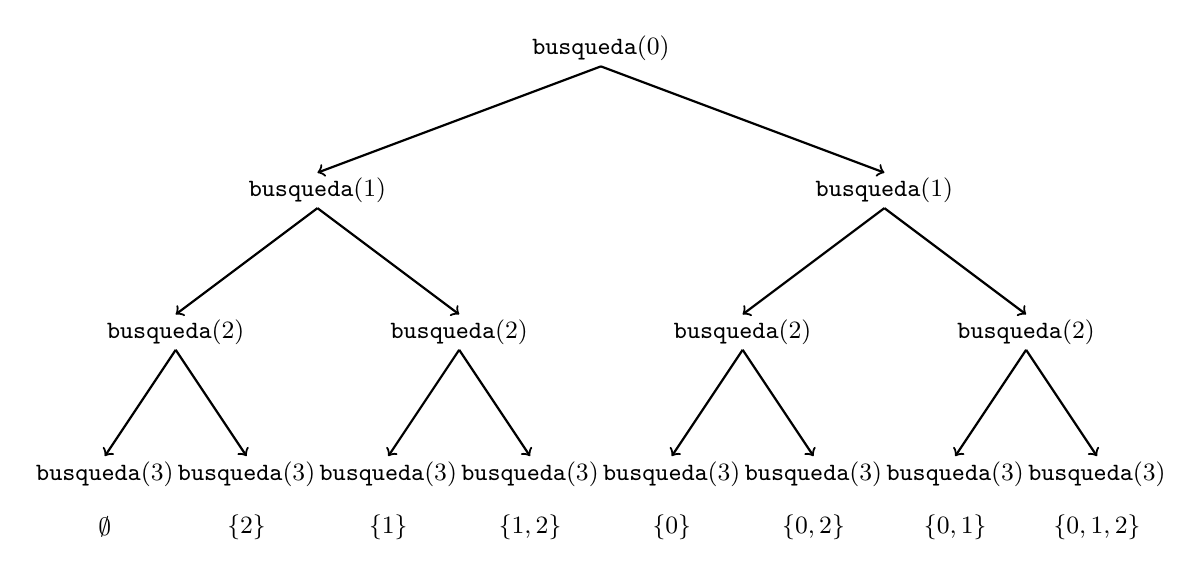
\begin{tikzpicture}[scale=.45]
  \begin{scope}
    \small
    \node at (0,0) {$\texttt{busqueda}(0)$};

    \node at (-8,-4) {$\texttt{busqueda}(1)$};
    \node at (8,-4) {$\texttt{busqueda}(1)$};

    \path[draw,thick,->] (0,0-0.5) -- (-8,-4+0.5);
    \path[draw,thick,->] (0,0-0.5) -- (8,-4+0.5);

    \node at (-12,-8) {$\texttt{busqueda}(2)$};
    \node at (-4,-8) {$\texttt{busqueda}(2)$};
    \node at (4,-8) {$\texttt{busqueda}(2)$};
    \node at (12,-8) {$\texttt{busqueda}(2)$};

    \path[draw,thick,->] (-8,-4-0.5) -- (-12,-8+0.5);
    \path[draw,thick,->] (-8,-4-0.5) -- (-4,-8+0.5);
    \path[draw,thick,->] (8,-4-0.5) -- (4,-8+0.5);
    \path[draw,thick,->] (8,-4-0.5) -- (12,-8+0.5);

    \node at (-14,-12) {$\texttt{busqueda}(3)$};
    \node at (-10,-12) {$\texttt{busqueda}(3)$};
    \node at (-6,-12) {$\texttt{busqueda}(3)$};
    \node at (-2,-12) {$\texttt{busqueda}(3)$};
    \node at (2,-12) {$\texttt{busqueda}(3)$};
    \node at (6,-12) {$\texttt{busqueda}(3)$};
    \node at (10,-12) {$\texttt{busqueda}(3)$};
    \node at (14,-12) {$\texttt{busqueda}(3)$};

    \node at (-14,-13.5) {$\emptyset$};
    \node at (-10,-13.5) {$\{2\}$};
    \node at (-6,-13.5) {$\{1\}$};
    \node at (-2,-13.5) {$\{1,2\}$};
    \node at (2,-13.5) {$\{0\}$};
    \node at (6,-13.5) {$\{0,2\}$};
    \node at (10,-13.5) {$\{0,1\}$};
    \node at (14,-13.5) {$\{0,1,2\}$};


    \path[draw,thick,->] (-12,-8-0.5) -- (-14,-12+0.5);
    \path[draw,thick,->] (-12,-8-0.5) -- (-10,-12+0.5);
    \path[draw,thick,->] (-4,-8-0.5) -- (-6,-12+0.5);
    \path[draw,thick,->] (-4,-8-0.5) -- (-2,-12+0.5);
    \path[draw,thick,->] (4,-8-0.5) -- (2,-12+0.5);
    \path[draw,thick,->] (4,-8-0.5) -- (6,-12+0.5);
    \path[draw,thick,->] (12,-8-0.5) -- (10,-12+0.5);
    \path[draw,thick,->] (12,-8-0.5) -- (14,-12+0.5);
\end{scope}
\end{tikzpicture}
\end{center}

\subsubsection{Method 2}

Another way to generate subsets is based on
the bit representation of integers.
Each subset of a set of $n$ elements
can be represented as a sequence of $n$ bits,
which corresponds to an integer between $0 \ldots 2^n-1$.
The ones in the bit sequence indicate
which elements are included in the subset.

The usual convention is that
the last bit corresponds to element 0,
the second last bit corresponds to element 1,
and so on.
For example, the bit representation of 25
is 11001, which corresponds to the subset $\{0,3,4\}$.

The following code goes through the subsets
of a set of $n$ elements

\begin{lstlisting}
for (int b = 0; b < (1<<n); b++) {
    // process subset
}
\end{lstlisting}

The following code shows how we can find
the elements of a subset that corresponds to a bit sequence.
When processing each subset,
the code builds a vector that contains the
elements in the subset.

\begin{lstlisting}
for (int b = 0; b < (1<<n); b++) {
    vector<int> subset;
    for (int i = 0; i < n; i++) {
        if (b&(1<<i)) subset.push_back(i);
    }
}
\end{lstlisting}

\section{Generating permutations}

\index{permutation}

Next we consider the problem of generating
all permutations of a set of $n$ elements.
For example, the permutations of $\{0,1,2\}$ are
$(0,1,2)$, $(0,2,1)$, $(1,0,2)$, $(1,2,0)$,
$(2,0,1)$ and $(2,1,0)$.
Again, there are two approaches:
we can either use recursion or go through the
permutations iteratively.

\subsubsection{Method 1}

Like subsets, permutations can be generated
using recursion.
The following function \texttt{search} goes
through the permutations of the set $\{0,1,\ldots,n-1\}$.
The function builds a vector \texttt{permutation}
that contains the permutation,
and the search begins when the function is
called without parameters.

\begin{lstlisting}
void search() {
    if (permutation.size() == n) {
        // process permutation
    } else {
        for (int i = 0; i < n; i++) {
            if (chosen[i]) continue;
            chosen[i] = true;
            permutation.push_back(i);
            search();
            chosen[i] = false;
            permutation.pop_back();
        }
    }
}
\end{lstlisting}

Each function call adds a new element to
\texttt{permutation}.
The array \texttt{chosen} indicates which
elements are already included in the permutation.
If the size of \texttt{permutation} equals the size of the set,
a permutation has been generated.

\subsubsection{Method 2}

\index{next\_permutation@\texttt{next\_permutation}}

Another method for generating permutations
is to begin with the permutation
$\{0,1,\ldots,n-1\}$ and repeatedly
use a function that constructs the next permutation
in increasing order.
The C++ standard library contains the function
\texttt{next\_permutation} that can be used for this:

\begin{lstlisting}
vector<int> permutation;
for (int i = 0; i < n; i++) {
    permutation.push_back(i);
}
do {
    // process permutation
} while (next_permutation(permutation.begin(),permutation.end()));
\end{lstlisting}

\section{Backtracking}

\index{backtracking}

A \key{backtracking} algorithm
begins with an empty solution
and extends the solution step by step.
The search recursively
goes through all different ways how
a solution can be constructed.

\index{queen problem}

As an example, consider the problem of
calculating the number
of ways $n$ queens can be placed on
an $n \times n$ chessboard so that
no two queens attack each other.
For example, when $n=4$,
there are two possible solutions:

\begin{center}
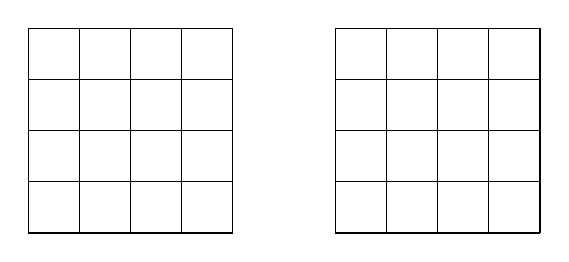
\begin{tikzpicture}[scale=.65]
  \begin{scope}
    \draw (0, 0) grid (4, 4);
    \node at (1.5,3.5) {\symqueen};
    \node at (3.5,2.5) {\symqueen};
    \node at (0.5,1.5) {\symqueen};
    \node at (2.5,0.5) {\symqueen};

    \draw (6, 0) grid (10, 4);
    \node at (6+2.5,3.5) {\symqueen};
    \node at (6+0.5,2.5) {\symqueen};
    \node at (6+3.5,1.5) {\symqueen};
    \node at (6+1.5,0.5) {\symqueen};

  \end{scope}
\end{tikzpicture}
\end{center}

The problem can be solved using backtracking
by placing queens to the board row by row.
More precisely, exactly one queen will
be placed on each row so that no queen attacks
any of the queens placed before.
A solution has been found when all
$n$ queens have been placed on the board.

For example, when $n=4$,
some partial solutions generated by
the backtracking algorithm are as follows:

\begin{center}
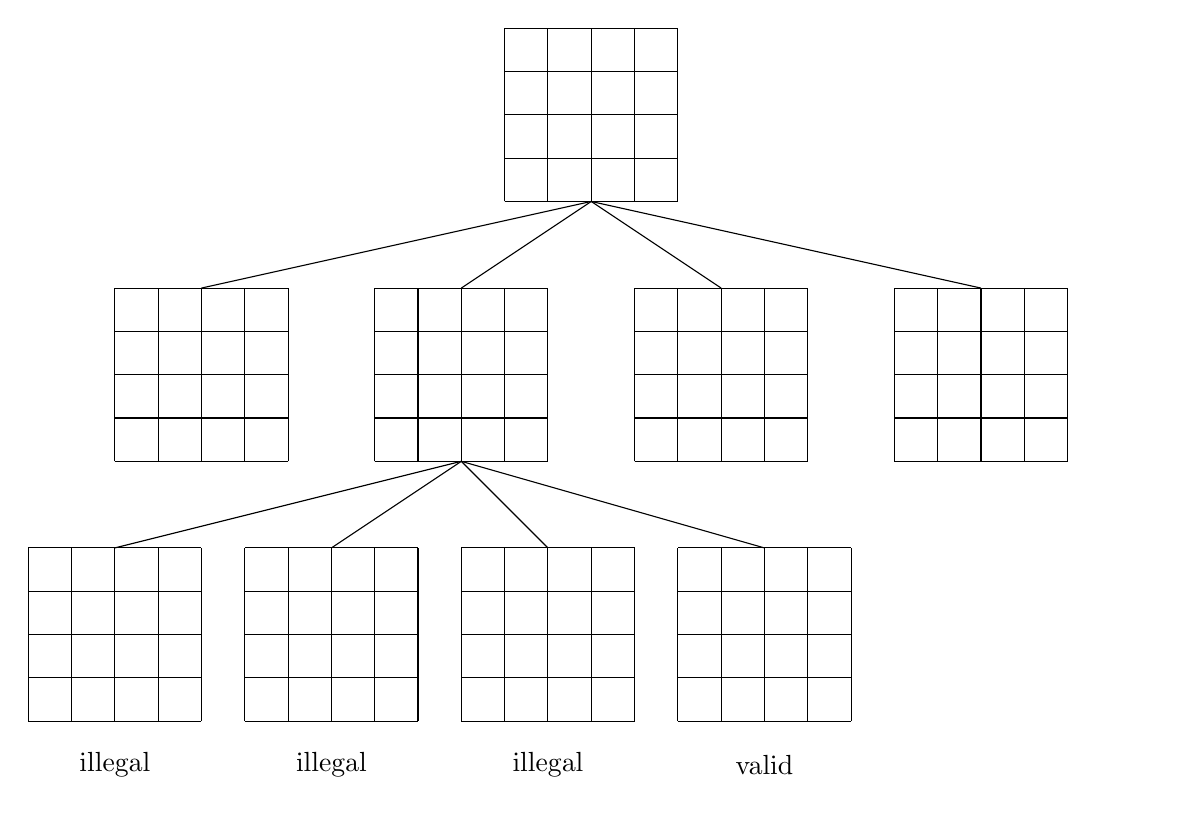
\begin{tikzpicture}[scale=.55]
  \begin{scope}
    \draw (0, 0) grid (4, 4);

    \draw (-9, -6) grid (-5, -2);
    \draw (-3, -6) grid (1, -2);
    \draw (3, -6) grid (7, -2);
    \draw (9, -6) grid (13, -2);

    \node at (-9+0.5,-3+0.5) {\symqueen};
    \node at (-3+1+0.5,-3+0.5) {\symqueen};
    \node at (3+2+0.5,-3+0.5) {\symqueen};
    \node at (9+3+0.5,-3+0.5) {\symqueen};

    \draw (2,0) -- (-7,-2);
    \draw (2,0) -- (-1,-2);
    \draw (2,0) -- (5,-2);
    \draw (2,0) -- (11,-2);

    \draw (-11, -12) grid (-7, -8);
    \draw (-6, -12) grid (-2, -8);
    \draw (-1, -12) grid (3, -8);
    \draw (4, -12) grid (8, -8);
    \draw[white] (11, -12) grid (15, -8);
    \node at (-11+1+0.5,-9+0.5) {\symqueen};
    \node at (-6+1+0.5,-9+0.5) {\symqueen};
    \node at (-1+1+0.5,-9+0.5) {\symqueen};
    \node at (4+1+0.5,-9+0.5) {\symqueen};
    \node at (-11+0+0.5,-10+0.5) {\symqueen};
    \node at (-6+1+0.5,-10+0.5) {\symqueen};
    \node at (-1+2+0.5,-10+0.5) {\symqueen};
    \node at (4+3+0.5,-10+0.5) {\symqueen};

    \draw (-1,-6) -- (-9,-8);
    \draw (-1,-6) -- (-4,-8);
    \draw (-1,-6) -- (1,-8);
    \draw (-1,-6) -- (6,-8);

    \node at (-9,-13) {illegal};
    \node at (-4,-13) {illegal};
    \node at (1,-13) {illegal};
    \node at (6,-13) {valid};

  \end{scope}
\end{tikzpicture}
\end{center}

At the bottom level, the three first configurations
are illegal, because the queens attack each other.
However, the fourth configuration is valid
and it can be extended to a complete solution by
placing two more queens to the board.
There is only one way to place the two remaining queens.

\begin{samepage}
The algorithm can be implemented as follows:
\begin{lstlisting}
void search(int y) {
    if (y == n) {
        count++;
        return;
    }
    for (int x = 0; x < n; x++) {
        if (column[x] || diag1[x+y] || diag2[x-y+n-1]) continue;
        column[x] = diag1[x+y] = diag2[x-y+n-1] = 1;
        search(y+1);
        column[x] = diag1[x+y] = diag2[x-y+n-1] = 0;
    }
}
\end{lstlisting}
\end{samepage}
The search begins by calling \texttt{search(0)}.
The size of the board is $n \times n$,
and the code calculates the number of solutions
to \texttt{count}.

The code assumes that the rows and columns
of the board are numbered from 0 to $n-1$.
When the function \texttt{search} is
called with parameter $y$,
it places a queen on row $y$
and then calls itself with parameter $y+1$.
Then, if $y=n$, a solution has been found
and the variable \texttt{count} is increased by one.

The array \texttt{column} keeps track of columns
that contain a queen,
and the arrays \texttt{diag1} and \texttt{diag2}
keep track of diagonals.
It is not allowed to add another queen to a
column or diagonal that already contains a queen. 
For example, the columns and diagonals of
the $4 \times 4$ board are numbered as follows:

\begin{center}
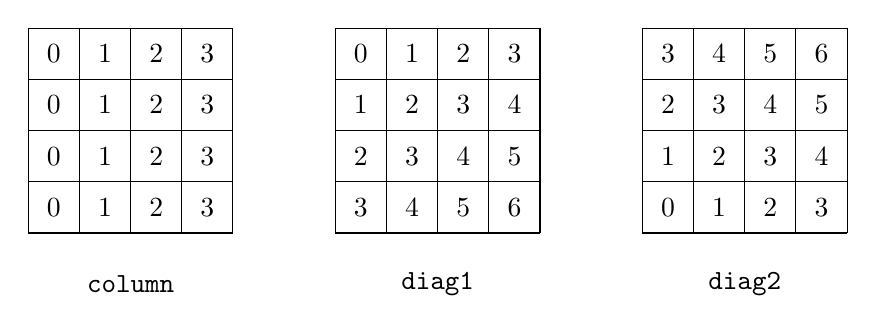
\begin{tikzpicture}[scale=.65]
  \begin{scope}
    \draw (0-6, 0) grid (4-6, 4);
    \node at (-6+0.5,3.5) {$0$};
    \node at (-6+1.5,3.5) {$1$};
    \node at (-6+2.5,3.5) {$2$};
    \node at (-6+3.5,3.5) {$3$};
    \node at (-6+0.5,2.5) {$0$};
    \node at (-6+1.5,2.5) {$1$};
    \node at (-6+2.5,2.5) {$2$};
    \node at (-6+3.5,2.5) {$3$};
    \node at (-6+0.5,1.5) {$0$};
    \node at (-6+1.5,1.5) {$1$};
    \node at (-6+2.5,1.5) {$2$};
    \node at (-6+3.5,1.5) {$3$};
    \node at (-6+0.5,0.5) {$0$};
    \node at (-6+1.5,0.5) {$1$};
    \node at (-6+2.5,0.5) {$2$};
    \node at (-6+3.5,0.5) {$3$};

    \draw (0, 0) grid (4, 4);
    \node at (0.5,3.5) {$0$};
    \node at (1.5,3.5) {$1$};
    \node at (2.5,3.5) {$2$};
    \node at (3.5,3.5) {$3$};
    \node at (0.5,2.5) {$1$};
    \node at (1.5,2.5) {$2$};
    \node at (2.5,2.5) {$3$};
    \node at (3.5,2.5) {$4$};
    \node at (0.5,1.5) {$2$};
    \node at (1.5,1.5) {$3$};
    \node at (2.5,1.5) {$4$};
    \node at (3.5,1.5) {$5$};
    \node at (0.5,0.5) {$3$};
    \node at (1.5,0.5) {$4$};
    \node at (2.5,0.5) {$5$};
    \node at (3.5,0.5) {$6$};

    \draw (6, 0) grid (10, 4);
    \node at (6.5,3.5) {$3$};
    \node at (7.5,3.5) {$4$};
    \node at (8.5,3.5) {$5$};
    \node at (9.5,3.5) {$6$};
    \node at (6.5,2.5) {$2$};
    \node at (7.5,2.5) {$3$};
    \node at (8.5,2.5) {$4$};
    \node at (9.5,2.5) {$5$};
    \node at (6.5,1.5) {$1$};
    \node at (7.5,1.5) {$2$};
    \node at (8.5,1.5) {$3$};
    \node at (9.5,1.5) {$4$};
    \node at (6.5,0.5) {$0$};
    \node at (7.5,0.5) {$1$};
    \node at (8.5,0.5) {$2$};
    \node at (9.5,0.5) {$3$};

    \node at (-4,-1) {\texttt{column}};
    \node at (2,-1) {\texttt{diag1}};
    \node at (8,-1) {\texttt{diag2}};

  \end{scope}
\end{tikzpicture}
\end{center}

Let $q(n)$ denote the number of ways
to place $n$ queens on an $n \times n$ chessboard.
The above backtracking
algorithm tells us that, for example, $q(8)=92$.
When $n$ increases, the search quickly becomes slow,
because the number of solutions increases
exponentially.
For example, calculating $q(16)=14772512$
using the above algorithm already takes about a minute
on a modern computer\footnote{There is no known way to efficiently
calculate larger values of $q(n)$. The current record is
$q(27)=234907967154122528$, calculated in 2016 \cite{q27}.}.

\section{Pruning the search}

We can often optimize backtracking
by pruning the search tree.
The idea is to add ''intelligence'' to the algorithm
so that it will notice as soon as possible
if a partial solution cannot be extended
to a complete solution.
Such optimizations can have a tremendous
effect on the efficiency of the search.

Let us consider the problem
of calculating the number of paths
in an $n \times n$ grid from the upper-left corner
to the lower-right corner such that the
path visits each square exactly once.
For example, in a $7 \times 7$ grid,
there are 111712 such paths.
One of the paths is as follows:

\begin{center}
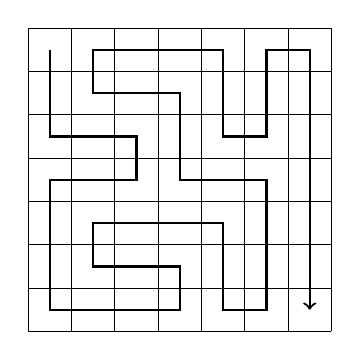
\begin{tikzpicture}[scale=.55]
  \begin{scope}
    \draw (0, 0) grid (7, 7);
    \draw[thick,->] (0.5,6.5) -- (0.5,4.5) -- (2.5,4.5) --
          (2.5,3.5) -- (0.5,3.5) -- (0.5,0.5) --
          (3.5,0.5) -- (3.5,1.5) -- (1.5,1.5) --
          (1.5,2.5) -- (4.5,2.5) -- (4.5,0.5) --
          (5.5,0.5) -- (5.5,3.5) -- (3.5,3.5) --
          (3.5,5.5) -- (1.5,5.5) -- (1.5,6.5) --
          (4.5,6.5) -- (4.5,4.5) -- (5.5,4.5) --
          (5.5,6.5) -- (6.5,6.5) -- (6.5,0.5);
  \end{scope}
\end{tikzpicture}
\end{center}

We focus on the $7 \times 7$ case,
because its level of difficulty is appropriate to our needs.
We begin with a straightforward backtracking algorithm,
and then optimize it step by step using observations
of how the search can be pruned.
After each optimization, we measure the running time
of the algorithm and the number of recursive calls,
so that we clearly see the effect of each
optimization on the efficiency of the search.

\subsubsection{Basic algorithm}

The first version of the algorithm does not contain
any optimizations. We simply use backtracking to generate
all possible paths from the upper-left corner to
the lower-right corner and count the number of such paths.

\begin{itemize}
\item
running time: 483 seconds
\item
number of recursive calls: 76 billion
\end{itemize}

\subsubsection{Optimization 1}

In any solution, we first move one step
down or right.
There are always two paths that 
are symmetric
about the diagonal of the grid
after the first step.
For example, the following paths are symmetric:

\begin{center}
\begin{tabular}{ccc}
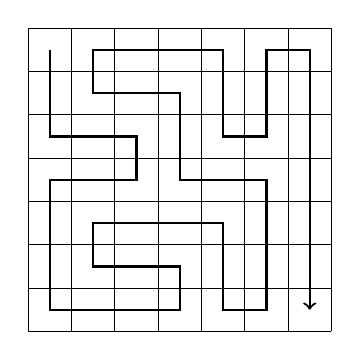
\begin{tikzpicture}[scale=.55]
  \begin{scope}
    \draw (0, 0) grid (7, 7);
    \draw[thick,->] (0.5,6.5) -- (0.5,4.5) -- (2.5,4.5) --
          (2.5,3.5) -- (0.5,3.5) -- (0.5,0.5) --
          (3.5,0.5) -- (3.5,1.5) -- (1.5,1.5) --
          (1.5,2.5) -- (4.5,2.5) -- (4.5,0.5) --
          (5.5,0.5) -- (5.5,3.5) -- (3.5,3.5) --
          (3.5,5.5) -- (1.5,5.5) -- (1.5,6.5) --
          (4.5,6.5) -- (4.5,4.5) -- (5.5,4.5) --
          (5.5,6.5) -- (6.5,6.5) -- (6.5,0.5);
  \end{scope}
\end{tikzpicture}
& \hspace{20px}
& 
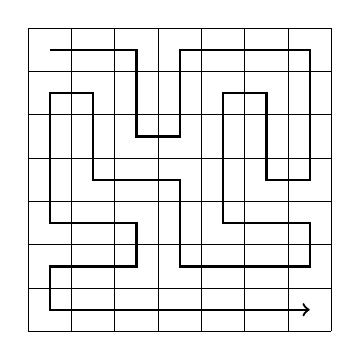
\begin{tikzpicture}[scale=.55]
  \begin{scope}[yscale=1,xscale=-1,rotate=-90]
    \draw (0, 0) grid (7, 7);
    \draw[thick,->] (0.5,6.5) -- (0.5,4.5) -- (2.5,4.5) --
          (2.5,3.5) -- (0.5,3.5) -- (0.5,0.5) --
          (3.5,0.5) -- (3.5,1.5) -- (1.5,1.5) --
          (1.5,2.5) -- (4.5,2.5) -- (4.5,0.5) --
          (5.5,0.5) -- (5.5,3.5) -- (3.5,3.5) --
          (3.5,5.5) -- (1.5,5.5) -- (1.5,6.5) --
          (4.5,6.5) -- (4.5,4.5) -- (5.5,4.5) --
          (5.5,6.5) -- (6.5,6.5) -- (6.5,0.5);
  \end{scope}
\end{tikzpicture}
\end{tabular}
\end{center}

Hence, we can decide that we always first
move one step down (or right),
and finally multiply the number of solutions by two.

\begin{itemize}
\item
running time: 244 seconds
\item
number of recursive calls: 38 billion
\end{itemize}

\subsubsection{Optimization 2}

If the path reaches the lower-right square
before it has visited all other squares of the grid,
it is clear that
it will not be possible to complete the solution.
An example of this is the following path:

\begin{center}
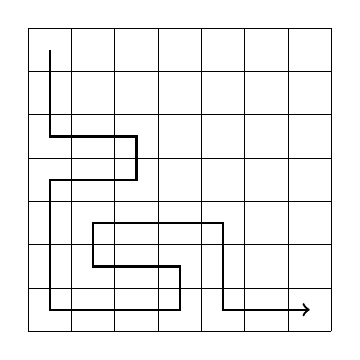
\begin{tikzpicture}[scale=.55]
  \begin{scope}
    \draw (0, 0) grid (7, 7);
    \draw[thick,->] (0.5,6.5) -- (0.5,4.5) -- (2.5,4.5) --
          (2.5,3.5) -- (0.5,3.5) -- (0.5,0.5) --
          (3.5,0.5) -- (3.5,1.5) -- (1.5,1.5) --
          (1.5,2.5) -- (4.5,2.5) -- (4.5,0.5) --
          (6.5,0.5);
  \end{scope}
\end{tikzpicture}
\end{center}
Using this observation, we can terminate the search
immediately if we reach the lower-right square too early.
\begin{itemize}
\item
running time: 119 seconds
\item
number of recursive calls: 20 billion
\end{itemize}

\subsubsection{Optimization 3}

If the path touches a wall
and can turn either left or right,
the grid splits into two parts
that contain unvisited squares.
For example, in the following situation,
the path can turn either left or right:

\begin{center}
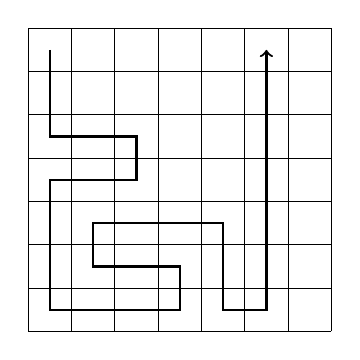
\begin{tikzpicture}[scale=.55]
  \begin{scope}
    \draw (0, 0) grid (7, 7);
    \draw[thick,->] (0.5,6.5) -- (0.5,4.5) -- (2.5,4.5) --
          (2.5,3.5) -- (0.5,3.5) -- (0.5,0.5) --
          (3.5,0.5) -- (3.5,1.5) -- (1.5,1.5) --
          (1.5,2.5) -- (4.5,2.5) -- (4.5,0.5) --
          (5.5,0.5) -- (5.5,6.5);
  \end{scope}
\end{tikzpicture}
\end{center}
In this case, we cannot visit all squares anymore,
so we can terminate the search.
This optimization is very useful:

\begin{itemize}
\item
running time: 1.8 seconds
\item
number of recursive calls: 221 million
\end{itemize}

\subsubsection{Optimization 4}

The idea of Optimization 3
can be generalized:
if the path cannot continue forward
but can turn either left or right,
the grid splits into two parts
that both contain unvisited squares.
For example, consider the following path:

\begin{center}
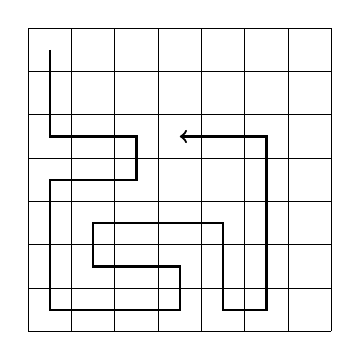
\begin{tikzpicture}[scale=.55]
  \begin{scope}
    \draw (0, 0) grid (7, 7);
    \draw[thick,->] (0.5,6.5) -- (0.5,4.5) -- (2.5,4.5) --
          (2.5,3.5) -- (0.5,3.5) -- (0.5,0.5) --
          (3.5,0.5) -- (3.5,1.5) -- (1.5,1.5) --
          (1.5,2.5) -- (4.5,2.5) -- (4.5,0.5) --
          (5.5,0.5) -- (5.5,4.5) -- (3.5,4.5);
  \end{scope}
\end{tikzpicture}
\end{center}
It is clear that we cannot visit all squares anymore,
so we can terminate the search.
After this optimization, the search is
very efficient:

\begin{itemize}
\item
running time: 0.6 seconds
\item
number of recursive calls: 69 million
\end{itemize}

~\\
Now is a good moment to stop optimizing
the algorithm and see what we have achieved.
The running time of the original algorithm
was 483 seconds,
and now after the optimizations,
the running time is only 0.6 seconds.
Thus, the algorithm became nearly 1000 times
faster after the optimizations.

This is a usual phenomenon in backtracking,
because the search tree is usually large
and even simple observations can effectively
prune the search.
Especially useful are optimizations that
occur during the first steps of the algorithm,
i.e., at the top of the search tree.

\section{Meet in the middle}

\index{meet in the middle}

\key{Meet in the middle} is a technique
where the search space is divided into
two parts of about equal size.
A separate search is performed
for both of the parts,
and finally the results of the searches are combined.

The technique can be used
if there is an efficient way to combine the
results of the searches.
In such a situation, the two searches may require less
time than one large search.
Typically, we can turn a factor of $2^n$
into a factor of $2^{n/2}$ using the meet in the
middle technique.

As an example, consider a problem where
we are given a list of $n$ numbers and
a number $x$,
and we want to find out if it is possible
to choose some numbers from the list so that
their sum is $x$.
For example, given the list $[2,4,5,9]$ and $x=15$,
we can choose the numbers $[2,4,9]$ to get $2+4+9=15$.
However, if $x=10$ for the same list,
it is not possible to form the sum.

A simple algorithm to the problem is to
go through all subsets of the elements and
check if the sum of any of the subsets is $x$.
The running time of such an algorithm is $O(2^n)$,
because there are $2^n$ subsets.
However, using the meet in the middle technique,
we can achieve a more efficient $O(2^{n/2})$ time algorithm\footnote{This
idea was introduced in 1974 by E. Horowitz and S. Sahni \cite{hor74}.}.
Note that $O(2^n)$ and $O(2^{n/2})$ are different
complexities because $2^{n/2}$ equals $\sqrt{2^n}$.

The idea is to divide the list into
two lists $A$ and $B$ such that both
lists contain about half of the numbers.
The first search generates all subsets
of $A$ and stores their sums to a list $S_A$.
Correspondingly, the second search creates
a list $S_B$ from $B$.
After this, it suffices to check if it is possible
to choose one element from $S_A$ and another
element from $S_B$ such that their sum is $x$.
This is possible exactly when there is a way to
form the sum $x$ using the numbers of the original list.

For example, suppose that the list is $[2,4,5,9]$ and $x=15$.
First, we divide the list into $A=[2,4]$ and $B=[5,9]$.
After this, we create lists
$S_A=[0,2,4,6]$ and $S_B=[0,5,9,14]$.
In this case, the sum $x=15$ is possible to form,
because $S_A$ contains the sum $6$,
$S_B$ contains the sum $9$, and $6+9=15$.
This corresponds to the solution $[2,4,9]$.

We can implement the algorithm so that
its time complexity is $O(2^{n/2})$.
First, we generate \emph{sorted} lists $S_A$ and $S_B$,
which can be done in $O(2^{n/2})$ time using a merge-like technique.
After this, since the lists are sorted,
we can check in $O(2^{n/2})$ time if
the sum $x$ can be created from $S_A$ and $S_B$.

\chapter{Algoritmos voraces}

\index{algoritmo voraz}

Un \key{algoritmo voraz}
construye una solución al problema
siempre tomando una elección que parece
ser la mejor en ese momento.
Un algoritmo voraz nunca revierte
sus elecciones, sino que construye directamente
la solución final.
Por esta razón, los algoritmos voraces
suelen ser muy eficientes.

La dificultad en el diseño de algoritmos voraces
es encontrar una estrategia voraz
que siempre produzca una solución óptima
al problema.
Las elecciones localmente óptimas en un algoritmo voraz
también deben ser óptimas a nivel global.
A menudo es difícil argumentar que
un algoritmo voraz funciona.

\section{Problema de monedas}

Como primer ejemplo, consideramos un problema
en el que se nos da un conjunto de monedas
y nuestra tarea es formar una suma de dinero $n$
usando las monedas.
Los valores de las monedas son
$\texttt{monedas}=\{c_1,c_2,\ldots,c_k\}$,
y cada moneda se puede usar tantas veces como queramos.
¿Cuál es el número mínimo de monedas necesario?

Por ejemplo, si las monedas son monedas de euro (en céntimos)
\[\{1,2,5,10,20,50,100,200\}\]
y $n=520$,
necesitamos al menos cuatro monedas.
La solución óptima es seleccionar las monedas
$200+200+100+20$ cuya suma es 520.

\subsubsection{Algoritmo voraz}

Un algoritmo voraz simple para el problema
siempre selecciona la moneda más grande posible,
hasta que se haya construido la suma de dinero requerida.
Este algoritmo funciona en el caso de ejemplo,
porque primero seleccionamos dos monedas de 200 céntimos,
luego una moneda de 100 céntimos y finalmente una moneda de 20 céntimos.
Pero, ¿siempre funciona este algoritmo?

Resulta que si las monedas son monedas de euro,
el algoritmo voraz \emph{siempre} funciona, es decir,
siempre produce una solución con el menor número
posible de monedas.
La corrección del algoritmo se puede
mostrar de la siguiente manera:

Primero, cada moneda 1, 5, 10, 50 y 100 aparece
como máximo una vez en una solución óptima,
porque si la
solución contuviera dos monedas de ese tipo,
podríamos reemplazarlas por una moneda y
obtener una solución mejor.
Por ejemplo, si la solución contuviera
monedas $5+5$, podríamos reemplazarlas por la moneda $10$.

De la misma manera, las monedas 2 y 20 aparecen
como máximo dos veces en una solución óptima,
porque podríamos reemplazar
monedas $2+2+2$ por monedas $5+1$ y
monedas $20+20+20$ por monedas $50+10$.
Además, una solución óptima no puede contener
monedas $2+2+1$ o $20+20+10$,
porque podríamos reemplazarlas por monedas de $5$ y $50$.

Usando estas observaciones,
podemos demostrar para cada moneda $x$ que
no es posible construir de manera óptima
una suma $x$ o cualquier suma mayor utilizando únicamente monedas
que sean más pequeñas que $x$.
Por ejemplo, si $x=100$, la suma óptima más grande
usando monedas más pequeñas es $50+20+20+5+2+2=99$.
Por lo tanto, el algoritmo voraz que siempre selecciona
la moneda más grande produce la solución óptima.

Este ejemplo muestra que puede ser difícil
argumentar que un algoritmo voraz funciona,
incluso si el algoritmo en sí es simple.

\subsubsection{Caso general}

En el caso general, el conjunto de monedas puede contener cualquier moneda
y el algoritmo voraz \emph{no} necesariamente produce
una solución óptima.

Podemos demostrar que un algoritmo voraz no funciona
mostrando un contraejemplo
donde el algoritmo proporciona una respuesta incorrecta.
En este problema, podemos encontrar fácilmente un contraejemplo:
si las monedas son $\{1,3,4\}$ y la suma objetivo
es 6, el algoritmo voraz produce la solución
$4+1+1$ mientras que la solución óptima es $3+3$.

No se sabe si el problema general de las monedas
se puede resolver utilizando algún algoritmo voraz\footnote{Sin embargo, es posible
\emph{verificar} en tiempo polinomial
si el algoritmo voraz presentado en este capítulo funciona para
un conjunto de monedas dado \cite{pea05}.}.
Sin embargo, como veremos en el Capítulo 7,
en algunos casos,
el problema general se puede resolver de manera eficiente
usando un algoritmo de programación dinámica que siempre proporciona la
respuesta correcta.

\section{Planificación}

Muchos problemas de planificación se pueden resolver
utilizando algoritmos voraces.
Un problema clásico es el siguiente:
Dado $n$ eventos con sus horas de inicio y finalización,
encuentra un horario
que incluya la mayor cantidad de eventos posible.
No es posible seleccionar un evento parcialmente.
Por ejemplo, considera los siguientes eventos:
\begin{center}
\begin{tabular}{lll}
evento & hora de inicio & hora de finalización \\
\hline
$A$ & 1 & 3 \\
$B$ & 2 & 5 \\
$C$ & 3 & 9 \\
$D$ & 6 & 8 \\
\end{tabular}
\end{center}
En este caso, el número máximo de eventos es dos.
Por ejemplo, podemos seleccionar los eventos $B$ y $D$
de la siguiente manera:
\begin{center}
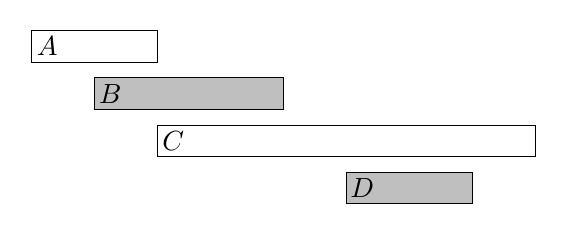
\begin{tikzpicture}[scale=.4]
  \begin{scope}
    \draw (2, 0) rectangle (6, -1);
    \draw[fill=lightgray] (4, -1.5) rectangle (10, -2.5);
    \draw (6, -3) rectangle (18, -4);
    \draw[fill=lightgray] (12, -4.5) rectangle (16, -5.5);
    \node at (2.5,-0.5) {$A$};
    \node at (4.5,-2) {$B$};
    \node at (6.5,-3.5) {$C$};
    \node at (12.5,-5) {$D$};
  \end{scope}
\end{tikzpicture}
\end{center}

Es posible inventar varios algoritmos voraces
para el problema, pero ¿cuál de ellos funciona en todos los casos?

\subsubsection*{Algoritmo 1}

La primera idea es seleccionar eventos lo más \emph{cortos}
posible.
En el caso de ejemplo, este algoritmo
selecciona los siguientes eventos:
\begin{center}
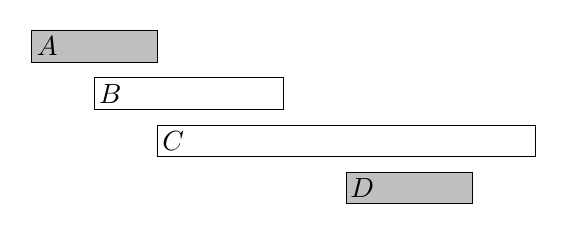
\begin{tikzpicture}[scale=.4]
  \begin{scope}
    \draw[fill=lightgray] (2, 0) rectangle (6, -1);
    \draw (4, -1.5) rectangle (10, -2.5);
    \draw (6, -3) rectangle (18, -4);
    \draw[fill=lightgray] (12, -4.5) rectangle (16, -5.5);
    \node at (2.5,-0.5) {$A$};
    \node at (4.5,-2) {$B$};
    \node at (6.5,-3.5) {$C$};
    \node at (12.5,-5) {$D$};
  \end{scope}
\end{tikzpicture}
\end{center}

Sin embargo, seleccionar eventos cortos no siempre
es una estrategia correcta. Por ejemplo, el algoritmo falla
en el siguiente caso:
\begin{center}
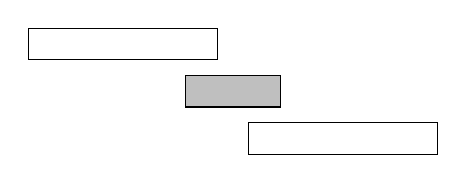
\begin{tikzpicture}[scale=.4]
  \begin{scope}
    \draw (1, 0) rectangle (7, -1);
    \draw[fill=lightgray] (6, -1.5) rectangle (9, -2.5);
    \draw (8, -3) rectangle (14, -4);
  \end{scope}
\end{tikzpicture}
\end{center}
Si seleccionamos el evento corto, solo podemos seleccionar un evento.
Sin embargo, sería posible seleccionar ambos eventos largos.

\subsubsection*{Algoritmo 2}

Otra idea es seleccionar siempre el siguiente evento posible
que \emph{comienza} lo más \emph{temprano} posible.
Este algoritmo selecciona los siguientes eventos:
\begin{center}
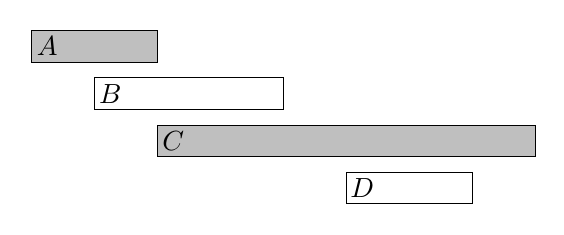
\begin{tikzpicture}[scale=.4]
  \begin{scope}
    \draw[fill=lightgray] (2, 0) rectangle (6, -1);
    \draw (4, -1.5) rectangle (10, -2.5);
    \draw[fill=lightgray] (6, -3) rectangle (18, -4);
    \draw (12, -4.5) rectangle (16, -5.5);
    \node at (2.5,-0.5) {$A$};
    \node at (4.5,-2) {$B$};
    \node at (6.5,-3.5) {$C$};
    \node at (12.5,-5) {$D$};
  \end{scope}
\end{tikzpicture}
\end{center}

Sin embargo, podemos encontrar un contraejemplo
también para este algoritmo.
Por ejemplo, en el siguiente caso,
el algoritmo solo selecciona un evento:
\begin{center}
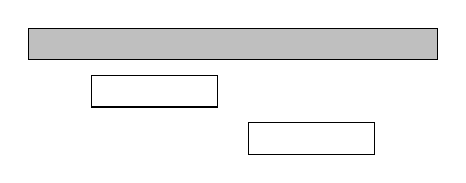
\begin{tikzpicture}[scale=.4]
  \begin{scope}
    \draw[fill=lightgray] (1, 0) rectangle (14, -1);
    \draw (3, -1.5) rectangle (7, -2.5);
    \draw (8, -3) rectangle (12, -4);
  \end{scope}
\end{tikzpicture}
\end{center}
Si seleccionamos el primer evento, no es posible
seleccionar ningún otro evento.
Sin embargo, sería posible seleccionar los
otros dos eventos.

\subsubsection*{Algoritmo 3}

La tercera idea es siempre seleccionar el siguiente
evento posible que \emph{termina} lo más \emph{temprano} posible.
Este algoritmo selecciona los siguientes eventos:
\begin{center}
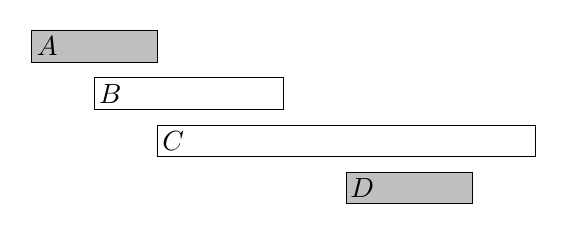
\begin{tikzpicture}[scale=.4]
  \begin{scope}
    \draw[fill=lightgray] (2, 0) rectangle (6, -1);
    \draw (4, -1.5) rectangle (10, -2.5);
    \draw (6, -3) rectangle (18, -4);
    \draw[fill=lightgray] (12, -4.5) rectangle (16, -5.5);
    \node at (2.5,-0.5) {$A$};
    \node at (4.5,-2) {$B$};
    \node at (6.5,-3.5) {$C$};
    \node at (12.5,-5) {$D$};
  \end{scope}
\end{tikzpicture}
\end{center}

Resulta que este algoritmo
\emph{siempre} produce una solución óptima.
La razón de esto es que siempre es una elección óptima
seleccionar primero un evento que termine
lo más temprano posible.
Después de esto, es una elección óptima
seleccionar el siguiente evento
usando la misma estrategia, etc.,
hasta que no podamos seleccionar más eventos.

Una forma de argumentar que el algoritmo funciona
es considerar
qué sucede si primero seleccionamos un evento
que termina más tarde que el evento que termina
lo más temprano posible.
Ahora, tendremos a lo sumo un número igual de
opciones de cómo podemos seleccionar el siguiente evento.
Por lo tanto, seleccionar un evento que termine más tarde
nunca puede generar una solución mejor,
y el algoritmo voraz es correcto.

\section{Tareas y tiempos límite}

Consideremos ahora un problema donde
se nos dan $n$ tareas con duraciones y tiempos límite
y nuestra tarea es elegir un orden para realizar las tareas.
Para cada tarea, ganamos $d-x$ puntos
donde $d$ es el tiempo límite de la tarea
y $x$ es el momento en que terminamos la tarea.
¿Cuál es el mayor puntaje total posible
que podemos obtener?

Por ejemplo, supongamos que las tareas son las siguientes:
\begin{center}
\begin{tabular}{lll}
tarea & duración & tiempo límite \\
\hline
$A$ & 4 & 2 \\
$B$ & 3 & 5 \\
$C$ & 2 & 7 \\
$D$ & 4 & 5 \\
\end{tabular}
\end{center}
En este caso, un programa óptimo para las tareas
es el siguiente:
\begin{center}
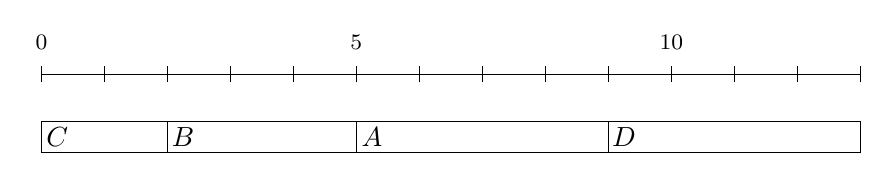
\begin{tikzpicture}[scale=.4]
  \begin{scope}
    \draw (0, 0) rectangle (4, -1);
    \draw (4, 0) rectangle (10, -1);
    \draw (10, 0) rectangle (18, -1);
    \draw (18, 0) rectangle (26, -1);
    \node at (0.5,-0.5) {$C$};
    \node at (4.5,-0.5) {$B$};
    \node at (10.5,-0.5) {$A$};
    \node at (18.5,-0.5) {$D$};

    \draw (0,1.5) -- (26,1.5);
    \foreach \i in {0,2,...,26}
    {
        \draw (\i,1.25) -- (\i,1.75);
    }
    \footnotesize
    \node at (0,2.5) {0};
    \node at (10,2.5) {5};
    \node at (20,2.5) {10};

  \end{scope}
\end{tikzpicture}
\end{center}
En esta solución, $C$ produce 5 puntos,
$B$ produce 0 puntos, $A$ produce $-7$ puntos
y $D$ produce $-8$ puntos,
entonces el puntaje total es $-10$.

Sorprendentemente, la solución óptima al problema
no depende de los tiempos límite en absoluto,
pero una estrategia voraz correcta es simplemente
realizar las tareas \emph{ordenadas por sus duraciones}
en orden creciente.
La razón de esto es que si alguna vez realizamos
dos tareas una tras otra de tal manera que la primera tarea
tarda más que la segunda tarea,
podemos obtener una mejor solución si intercambiamos las tareas.
Por ejemplo, considere el siguiente horario:
\begin{center}
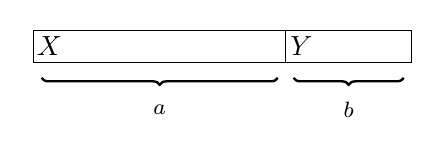
\begin{tikzpicture}[scale=.4]
  \begin{scope}
    \draw (0, 0) rectangle (8, -1);
    \draw (8, 0) rectangle (12, -1);
    \node at (0.5,-0.5) {$X$};
    \node at (8.5,-0.5) {$Y$};

\draw [decoration={brace}, decorate, line width=0.3mm] (7.75,-1.5) -- (0.25,-1.5);
\draw [decoration={brace}, decorate, line width=0.3mm] (11.75,-1.5) -- (8.25,-1.5);

\footnotesize
\node at (4,-2.5) {$a$};
\node at (10,-2.5) {$b$};

  \end{scope}
\end{tikzpicture}
\end{center}
Aquí $a>b$, entonces deberíamos intercambiar las tareas:
\begin{center}
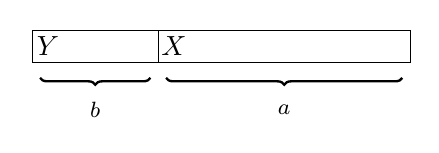
\begin{tikzpicture}[scale=.4]
  \begin{scope}
    \draw (0, 0) rectangle (4, -1);
    \draw (4, 0) rectangle (12, -1);
    \node at (0.5,-0.5) {$Y$};
    \node at (4.5,-0.5) {$X$};

\draw [decoration={brace}, decorate, line width=0.3mm] (3.75,-1.5) -- (0.25,-1.5);
\draw [decoration={brace}, decorate, line width=0.3mm] (11.75,-1.5) -- (4.25,-1.5);

\footnotesize
\node at (2,-2.5) {$b$};
\node at (8,-2.5) {$a$};

  \end{scope}
\end{tikzpicture}
\end{center}
Ahora $X$ otorga $b$ puntos menos y $Y$ otorga $a$ puntos más,
entonces el puntaje total aumenta en $a-b > 0$.
En una solución óptima,
para cualquier par de tareas consecutivas,
debe cumplirse que la tarea más corta venga
antes que la tarea más larga.
Por lo tanto, las tareas deben realizarse
ordenadas por sus duraciones.

\section{Minimizando sumas}

A continuación, consideramos un problema en el que
se nos dan $n$ números $a_1,a_2,\ldots,a_n$
y nuestra tarea es encontrar un valor $x$
que minimice la suma
\[|a_1-x|^c+|a_2-x|^c+\cdots+|a_n-x|^c.\]
Nos enfocamos en los casos $c=1$ y $c=2$.

\subsubsection{Caso $c=1$}

En este caso, debemos minimizar la suma
\[|a_1-x|+|a_2-x|+\cdots+|a_n-x|.\]
Por ejemplo, si los números son $[1,2,9,2,6]$,
la mejor solución es seleccionar $x=2$
que produce la suma
\[
|1-2|+|2-2|+|9-2|+|2-2|+|6-2|=12.
\]
En el caso general, la mejor opción para $x$
es la \textit{mediana} de los números,
es decir, el número del medio después de ordenar.
Por ejemplo, la lista $[1,2,9,2,6]$
se convierte en $[1,2,2,6,9]$ después de ordenar,
así que la mediana es 2.

La mediana es una elección óptima,
porque si $x$ es menor que la mediana,
la suma se vuelve más pequeña al aumentar $x$,
y si $x$ es mayor que la mediana,
la suma se vuelve más pequeña al disminuir $x$.
Por lo tanto, la solución óptima es que $x$
sea la mediana.
Si $n$ es par y hay dos medianas,
ambas medianas y todos los valores entre ellas
son opciones óptimas.

\subsubsection{Caso $c=2$}

En este caso, debemos minimizar la suma
\[(a_1-x)^2+(a_2-x)^2+\cdots+(a_n-x)^2.\]
Por ejemplo, si los números son $[1,2,9,2,6]$,
la mejor solución es seleccionar $x=4$
que produce la suma
\[
(1-4)^2+(2-4)^2+(9-4)^2+(2-4)^2+(6-4)^2=46.
\]
En el caso general, la mejor opción para $x$
es el \emph{promedio} de los números.
En el ejemplo, el promedio es $(1+2+9+2+6)/5=4$.
Este resultado se puede derivar presentando
la suma de la siguiente manera:
\[
nx^2 - 2x(a_1+a_2+\cdots+a_n) + (a_1^2+a_2^2+\cdots+a_n^2)
\]
La última parte no depende de $x$,
así que podemos ignorarla.
Las partes restantes forman una función
$nx^2-2xs$ donde $s=a_1+a_2+\cdots+a_n$.
Esta es una parábola que se abre hacia arriba
con raíces $x=0$ y $x=2s/n$,
y el valor mínimo es el promedio
de las raíces $x=s/n$, es decir,
el promedio de los números $a_1,a_2,\ldots,a_n$.

\section{Compresión de datos}

\index{compresión de datos}
\index{código binario}
\index{palabra clave}

Un \key{código binario} asigna para cada carácter
de una cadena una \key{palabra clave} que consiste en bits.
Podemos \emph{comprimir} la cadena usando el código binario
sustituyendo cada carácter por la
palabra clave correspondiente.
Por ejemplo, el siguiente código binario
asigna palabras clave para los caracteres
\texttt{A}–\texttt{D}:
\begin{center}
\begin{tabular}{rr}
carácter & palabra clave \\
\hline
\texttt{A} & 00 \\
\texttt{B} & 01 \\
\texttt{C} & 10 \\
\texttt{D} & 11 \\
\end{tabular}
\end{center}
Este es un \key{código de longitud constante}
lo que significa que la longitud de cada
palabra clave es la misma.
Por ejemplo, podemos comprimir la cadena
\texttt{AABACDACA} de la siguiente manera:
\[00\,00\,01\,00\,10\,11\,00\,10\,00\]
Usando este código, la longitud de la cadena comprimida
es de 18 bits.
Sin embargo, podemos comprimir mejor la cadena
si utilizamos un \key{código de longitud variable}
donde las palabras clave pueden tener longitudes diferentes.
Entonces podemos dar palabras clave cortas para
caracteres que aparecen a menudo
y palabras clave largas para caracteres
que aparecen raramente.
Resulta que un \key{código óptimo}
para la cadena anterior es el siguiente:
\begin{center}
\begin{tabular}{rr}
carácter & palabra clave \\
\hline
\texttt{A} & 0 \\
\texttt{B} & 110 \\
\texttt{C} & 10 \\
\texttt{D} & 111 \\
\end{tabular}
\end{center}
Un código óptimo produce una cadena comprimida
que es lo más corta posible.
En este caso, la cadena comprimida usando
el código óptimo es
\[0\,0\,110\,0\,10\,111\,0\,10\,0,\]
así que solo se necesitan 15 bits en lugar de 18 bits.
Por lo tanto, gracias a un código mejor fue posible
ahorrar 3 bits en la cadena comprimida.

Se requiere que ninguna palabra clave
sea un prefijo de otra palabra clave.
Por ejemplo, no está permitido que un código
contenga tanto las palabras clave 10
como 1011.
La razón de esto es que queremos
poder generar la cadena original
a partir de la cadena comprimida.
Si una palabra clave pudiera ser un prefijo de otra palabra clave,
esto no siempre sería posible.
Por ejemplo, el siguiente código \emph{no} es válido:
\begin{center}
\begin{tabular}{rr}
carácter & palabra clave \\
\hline
\texttt{A} & 10 \\
\texttt{B} & 11 \\
\texttt{C} & 1011 \\
\texttt{D} & 111 \\
\end{tabular}
\end{center}
Usando este código, no sería posible saber
si la cadena comprimida 1011 corresponde a
la cadena \texttt{AB} o la cadena \texttt{C}.

\index{Codificación de Huffman}

\subsubsection{Codificación de Huffman}

La \key{Codificación de Huffman}\footnote{D. A. Huffman descubrió este método
al resolver una tarea de un curso universitario
y publicó el algoritmo en 1952 \cite{huf52}.} es un algoritmo voraz
que construye un código óptimo para
comprimir una cadena dada.
El algoritmo construye un árbol binario
basado en las frecuencias de los caracteres
en la cadena,
y el código de cada carácter se puede leer
siguiendo un camino desde la raíz hasta
el nodo correspondiente.
Un movimiento a la izquierda corresponde al bit 0,
y un movimiento a la derecha corresponde al bit 1.

Inicialmente, cada carácter de la cadena es
representado por un nodo cuyo peso es la
cantidad de veces que el carácter aparece en la cadena.
Luego, en cada paso, se combinan dos nodos con pesos mínimos
creando un nuevo nodo cuyo peso es la suma de los pesos
de los nodos originales.
El proceso continúa hasta que todos los nodos se hayan combinado.

Next we will see how Huffman coding creates
the optimal code for the string
\texttt{AABACDACA}.
Initially, there are four nodes that correspond
to the characters of the string:

\begin{center}
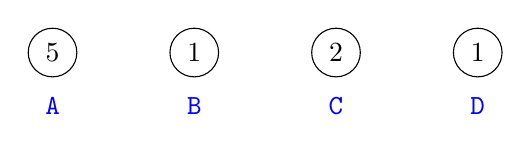
\begin{tikzpicture}[scale=0.9]
\node[draw, circle] (1) at (0,0) {$5$};
\node[draw, circle] (2) at (2,0) {$1$};
\node[draw, circle] (3) at (4,0) {$2$};
\node[draw, circle] (4) at (6,0) {$1$};

\node[color=blue] at (0,-0.75) {\texttt{A}};
\node[color=blue] at (2,-0.75) {\texttt{B}};
\node[color=blue] at (4,-0.75) {\texttt{C}};
\node[color=blue] at (6,-0.75) {\texttt{D}};

%\path[draw,thick,-] (4) -- (5);
\end{tikzpicture}
\end{center}
The node that represents character \texttt{A}
has weight 5 because character \texttt{A}
appears 5 times in the string.
The other weights have been calculated
in the same way.

The first step is to combine the nodes that
correspond to characters \texttt{B} and \texttt{D},
both with weight 1.
The result is:
\begin{center}
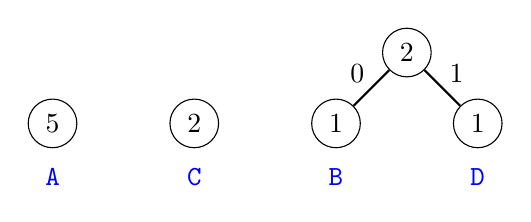
\begin{tikzpicture}[scale=0.9]
\node[draw, circle] (1) at (0,0) {$5$};
\node[draw, circle] (3) at (2,0) {$2$};
\node[draw, circle] (2) at (4,0) {$1$};
\node[draw, circle] (4) at (6,0) {$1$};
\node[draw, circle] (5) at (5,1) {$2$};

\node[color=blue] at (0,-0.75) {\texttt{A}};
\node[color=blue] at (2,-0.75) {\texttt{C}};
\node[color=blue] at (4,-0.75) {\texttt{B}};
\node[color=blue] at (6,-0.75) {\texttt{D}};

\node at (4.3,0.7) {0};
\node at (5.7,0.7) {1};

\path[draw,thick,-] (2) -- (5);
\path[draw,thick,-] (4) -- (5);
\end{tikzpicture}
\end{center}
After this, the nodes with weight 2 are combined:
\begin{center}
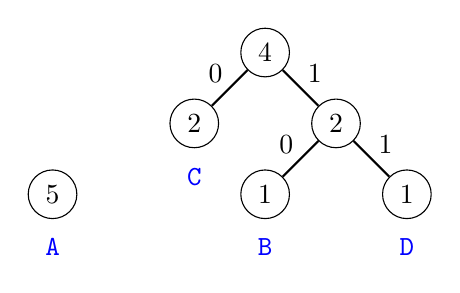
\begin{tikzpicture}[scale=0.9]
\node[draw, circle] (1) at (1,0) {$5$};
\node[draw, circle] (3) at (3,1) {$2$};
\node[draw, circle] (2) at (4,0) {$1$};
\node[draw, circle] (4) at (6,0) {$1$};
\node[draw, circle] (5) at (5,1) {$2$};
\node[draw, circle] (6) at (4,2) {$4$};

\node[color=blue] at (1,-0.75) {\texttt{A}};
\node[color=blue] at (3,1-0.75) {\texttt{C}};
\node[color=blue] at (4,-0.75) {\texttt{B}};
\node[color=blue] at (6,-0.75) {\texttt{D}};

\node at (4.3,0.7) {0};
\node at (5.7,0.7) {1};
\node at (3.3,1.7) {0};
\node at (4.7,1.7) {1};

\path[draw,thick,-] (2) -- (5);
\path[draw,thick,-] (4) -- (5);
\path[draw,thick,-] (3) -- (6);
\path[draw,thick,-] (5) -- (6);
\end{tikzpicture}
\end{center}
Finally, the two remaining nodes are combined:
\begin{center}
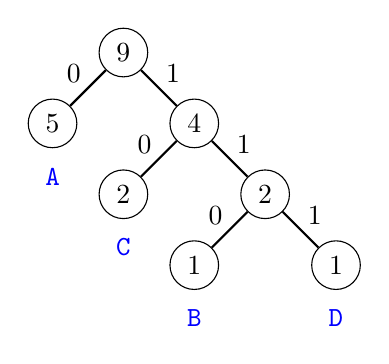
\begin{tikzpicture}[scale=0.9]
\node[draw, circle] (1) at (2,2) {$5$};
\node[draw, circle] (3) at (3,1) {$2$};
\node[draw, circle] (2) at (4,0) {$1$};
\node[draw, circle] (4) at (6,0) {$1$};
\node[draw, circle] (5) at (5,1) {$2$};
\node[draw, circle] (6) at (4,2) {$4$};
\node[draw, circle] (7) at (3,3) {$9$};

\node[color=blue] at (2,2-0.75) {\texttt{A}};
\node[color=blue] at (3,1-0.75) {\texttt{C}};
\node[color=blue] at (4,-0.75) {\texttt{B}};
\node[color=blue] at (6,-0.75) {\texttt{D}};

\node at (4.3,0.7) {0};
\node at (5.7,0.7) {1};
\node at (3.3,1.7) {0};
\node at (4.7,1.7) {1};
\node at (2.3,2.7) {0};
\node at (3.7,2.7) {1};

\path[draw,thick,-] (2) -- (5);
\path[draw,thick,-] (4) -- (5);
\path[draw,thick,-] (3) -- (6);
\path[draw,thick,-] (5) -- (6);
\path[draw,thick,-] (1) -- (7);
\path[draw,thick,-] (6) -- (7);
\end{tikzpicture}
\end{center}

Now all nodes are in the tree, so the code is ready.
The following codewords can be read from the tree:
\begin{center}
\begin{tabular}{rr}
character & codeword \\
\hline
\texttt{A} & 0 \\
\texttt{B} & 110 \\
\texttt{C} & 10 \\
\texttt{D} & 111 \\
\end{tabular}
\end{center}

\chapter{Programación dinámica}

\index{programación dinámica}

\key{Programación dinámica}
es una técnica que combina la correctitud
de la búsqueda completa y la eficiencia
de los algoritmos voraces.
La programación dinámica se puede aplicar si el
problema se puede dividir en subproblemas superpuestos
que se pueden resolver de forma independiente.

Hay dos usos para la programación dinámica:

\begin{itemize}
\item
\key{Encontrar una solución óptima}:
Queremos encontrar una solución que sea
lo más grande posible o lo más pequeña posible.
\item
\key{Contar el número de soluciones}:
Queremos calcular el número total de
soluciones posibles.
\end{itemize}

Primero veremos cómo la programación dinámica puede
usarse para encontrar una solución óptima,
y luego usaremos la misma idea para
contar las soluciones.

Entender la programación dinámica es un hito
en la carrera de todo programador competitivo.
Si bien la idea básica es simple,
el desafío es cómo aplicar
la programación dinámica a diferentes problemas.
Este capítulo presenta un conjunto de problemas clásicos
que son un buen punto de partida.

\section{Problema de las monedas}

Primero nos enfocamos en un problema que ya
hemos visto en el Capítulo 6:
Dado un conjunto de valores de monedas $\texttt{monedas} = \{c_1,c_2,\ldots,c_k\}$
y una suma objetivo de dinero $n$, nuestra tarea es
formar la suma $n$ usando la menor cantidad de monedas posible.

En el Capítulo 6, resolvimos el problema usando un
algoritmo voraz que siempre elige la moneda
más grande posible.
El algoritmo voraz funciona, por ejemplo,
cuando las monedas son las monedas de euro,
pero en el caso general, el algoritmo voraz
no necesariamente produce una solución óptima.

Ahora es el momento de resolver el problema de manera eficiente
usando programación dinámica, de modo que el algoritmo
funcione para cualquier conjunto de monedas.
El algoritmo de programación dinámica
se basa en una función recursiva
que analiza todas las posibilidades de cómo
formar la suma, como un algoritmo de fuerza bruta.
Sin embargo, el algoritmo de programación dinámica
es eficiente porque
utiliza \emph{memoización} y
calcula la respuesta a cada subproblema solo una vez.

\subsubsection{Formulación recursiva}

La idea en la programación dinámica es
formular el problema de manera recursiva para que
la solución al problema se pueda
calcular a partir de soluciones a problemas
más pequeños.
En el problema de las monedas, un problema recursivo
natural es el siguiente:
¿cuál es el menor número de monedas
requeridas para formar una suma $x$?

Denotemos $\texttt{resolver}(x)$
como el mínimo
número de monedas requeridas para una suma $x$.
Los valores de la función dependen de los
valores de las monedas.
Por ejemplo, si $\texttt{monedas} = \{1,3,4\}$,
los primeros valores de la función son los siguientes:

\[
\begin{array}{lcl}
\texttt{resolver}(0) & = & 0 \\
\texttt{resolver}(1) & = & 1 \\
\texttt{resolver}(2) & = & 2 \\
\texttt{resolver}(3) & = & 1 \\
\texttt{resolver}(4) & = & 1 \\
\texttt{resolver}(5) & = & 2 \\
\texttt{resolver}(6) & = & 2 \\
\texttt{resolver}(7) & = & 2 \\
\texttt{resolver}(8) & = & 2 \\
\texttt{resolver}(9) & = & 3 \\
\texttt{resolver}(10) & = & 3 \\
\end{array}
\]

Por ejemplo, $\texttt{resolver}(10)=3$,
porque se necesitan al menos 3 monedas
para formar la suma 10.
La solución óptima es $3+3+4=10$.

La propiedad esencial de $\texttt{resolver}$ es
que sus valores se pueden
calcular recursivamente a partir de sus valores más pequeños.
La idea es centrarse en la \emph{primera}
moneda que elegimos para la suma.
Por ejemplo, en el escenario anterior,
la primera moneda puede ser 1, 3 o 4.
Si primero elegimos la moneda 1,
la tarea restante es formar la suma 9
usando el mínimo número de monedas,
lo cual es un subproblema del problema original.
Por supuesto, lo mismo se aplica a las monedas 3 y 4.
Así, podemos usar la siguiente fórmula recursiva
para calcular el mínimo número de monedas:
\begin{equation*}
\begin{split}
\texttt{resolver}(x) = \min( & \texttt{resolver}(x-1)+1, \\
                           & \texttt{resolver}(x-3)+1, \\
                           & \texttt{resolver}(x-4)+1).
\end{split}
\end{equation*}
El caso base de la recursión es $\texttt{resolver}(0)=0$,
porque no se necesitan monedas para formar una suma vacía.
Por ejemplo,
\[ \texttt{resolver}(10) = \texttt{resolver}(7)+1 = \texttt{resolver}(4)+2 = \texttt{resolver}(0)+3 = 3.\]

Ahora estamos listos para dar una función recursiva general
que calcule el mínimo número de
monedas necesarias para formar una suma $x$:
\begin{equation*}
    \texttt{resolver}(x) = \begin{cases}
               \infty               & x < 0\\
               0               & x = 0\\
               \min_{c \in \texttt{monedas}} \texttt{resolver}(x-c)+1 & x > 0 \\
           \end{cases}
\end{equation*}

Primero, si $x<0$, el valor es $\infty$,
porque es imposible formar una suma
negativa de dinero.
Luego, si $x=0$, el valor es $0$,
porque no se necesitan monedas para formar una suma vacía.
Finalmente, si $x>0$, la variable $c$ recorre
todas las posibilidades de cómo elegir la primera moneda
de la suma.

Una vez que se encuentra una función recursiva que resuelve el problema,
podemos implementar directamente una solución en C++
(la constante \texttt{INF} denota infinito):

\begin{lstlisting}
int resolver(int x) {
    if (x < 0) return INF;
    if (x == 0) return 0;
    int mejor = INF;
    for (auto c : monedas) {
        mejor = min(mejor, resolver(x-c)+1);
    }
    return mejor;
}
\end{lstlisting}

Sin embargo, esta función no es eficiente,
porque puede haber un número exponencial de formas
de construir la suma.
No obstante, a continuación veremos cómo hacer que la
función sea eficiente utilizando una técnica llamada memoización.

\subsubsection{Usando memoización}

\index{memoización}

La idea de la programación dinámica es utilizar
\key{memoización} para calcular eficientemente
los valores de una función recursiva.
Esto significa que los valores de la función
se almacenan en un arreglo después de calcularlos.
Para cada parámetro, el valor de la función
se calcula recursivamente solo una vez y, después de esto,
el valor se puede recuperar directamente del arreglo.

En este problema, usamos los arreglos
\begin{lstlisting}
bool listo[N];
int valor[N];
\end{lstlisting}

donde $\texttt{listo}[x]$ indica
si se ha calculado el valor de $\texttt{resolver}(x)$,
y si lo está, $\texttt{valor}[x]$
contiene este valor.
La constante $N$ se ha elegido de manera que
todos los valores requeridos quepan en los arreglos.

Ahora la función se puede implementar de manera eficiente de la siguiente forma:

\begin{lstlisting}
int resolver(int x) {
    if (x < 0) return INF;
    if (x == 0) return 0;
    if (listo[x]) return valor[x];
    int mejor = INF;
    for (auto c : monedas) {
        mejor = min(mejor, resolver(x-c)+1);
    }
    valor[x] = mejor;
    listo[x] = true;
    return mejor;
}
\end{lstlisting}

La función maneja los casos base
$x<0$ y $x=0$ como antes.
Luego, la función verifica en
$\texttt{listo}[x]$ si
$\texttt{resolver}(x)$ ya ha sido almacenado
en $\texttt{valor}[x]$,
y si es así, la función lo devuelve directamente.
De lo contrario, la función calcula el valor
de $\texttt{resolver}(x)$
recursivamente y lo almacena en $\texttt{valor}[x]$.

Esta función funciona de manera eficiente,
porque la respuesta para cada parámetro $x$
se calcula recursivamente solo una vez.
Después de que se haya almacenado un valor de $\texttt{resolver}(x)$ en $\texttt{valor}[x]$,
se puede recuperar de manera eficiente cada vez que
la función sea llamada nuevamente con el parámetro $x$.
La complejidad en tiempo del algoritmo es $O(nk)$,
donde $n$ es la suma objetivo y $k$ es el número de monedas.

También podemos construir \emph{iterativamente}
el arreglo \texttt{valor} usando
un bucle que simplemente calcule todos los valores
de $\texttt{resolver}$ para los parámetros $0 \ldots n$:
\begin{lstlisting}
valor[0] = 0;
for (int x = 1; x <= n; x++) {
    valor[x] = INF;
    for (auto c : monedas) {
        if (x-c >= 0) {
            valor[x] = min(valor[x], valor[x-c]+1);
        }
    }
}
\end{lstlisting}

De hecho, la mayoría de los programadores competitivos prefieren esta
implementación, porque es más corta y tiene
factores constantes más bajos.
A partir de ahora, también utilizamos implementaciones iterativas
en nuestros ejemplos.
Aun así, a menudo es más fácil pensar en soluciones
de programación dinámica
en términos de funciones recursivas.


\subsubsection{Construyendo una solución}

A veces se nos pide encontrar el valor
de una solución óptima y dar
un ejemplo de cómo se puede construir dicha solución.
En el problema de las monedas, por ejemplo,
podemos declarar otro arreglo
que indique para
cada suma de dinero la primera moneda
en una solución óptima:
\begin{lstlisting}
int primero[N];
\end{lstlisting}
Luego, podemos modificar el algoritmo de la siguiente manera:
\begin{lstlisting}
valor[0] = 0;
for (int x = 1; x <= n; x++) {
    valor[x] = INF;
    for (auto c : monedas) {
        if (x-c >= 0 && valor[x-c]+1 < valor[x]) {
            valor[x] = valor[x-c]+1;
            primero[x] = c;
        }
    }
}
\end{lstlisting}
Después de esto, el siguiente código se puede utilizar para
imprimir las monedas que aparecen en una solución óptima para
la suma $n$:
\begin{lstlisting}
while (n > 0) {
    cout << primero[n] << "\n";
    n -= primero[n];
}
\end{lstlisting}

\subsubsection{Contando el número de soluciones}

Ahora consideremos otra versión
del problema de las monedas donde nuestra tarea es
calcular el número total de formas
de obtener una suma $x$ usando las monedas.
Por ejemplo, si $\texttt{monedas}=\{1,3,4\}$ y
$x=5$, hay un total de 6 formas:

\begin{multicols}{2}
\begin{itemize}
\item $1+1+1+1+1$
\item $1+1+3$
\item $1+3+1$
\item $3+1+1$
\item $1+4$
\item $4+1$
\end{itemize}
\end{multicols}

De nuevo, podemos resolver el problema recursivamente.
Sea $\texttt{resolver}(x)$ el número de formas
en las que podemos formar la suma $x$.
Por ejemplo, si $\texttt{monedas}=\{1,3,4\}$,
entonces $\texttt{resolver}(5)=6$ y la fórmula recursiva es
\begin{equation*}
\begin{split}
\texttt{resolver}(x) = & \texttt{resolver}(x-1) + \\
                    & \texttt{resolver}(x-3) + \\
                    & \texttt{resolver}(x-4)  .
\end{split}
\end{equation*}

Entonces, la función recursiva general es la siguiente:
\begin{equation*}
    \texttt{resolver}(x) = \begin{cases}
               0               & x < 0\\
               1               & x = 0\\
               \sum_{c \in \texttt{monedas}} \texttt{resolver}(x-c) & x > 0 \\
           \end{cases}
\end{equation*}

Si $x<0$, el valor es 0, porque no hay soluciones.
Si $x=0$, el valor es 1, porque solo hay una forma
de formar una suma vacía.
De lo contrario, calculamos la suma de todos los valores
de la forma $\texttt{resolver}(x-c)$ donde $c$ está en \texttt{monedas}.

El siguiente código construye un array
$\texttt{conteo}$ tal que
$\texttt{conteo}[x]$ es igual
al valor de $\texttt{resolver}(x)$
para $0 \le x \le n$:

\begin{lstlisting}
conteo[0] = 1;
for (int x = 1; x <= n; x++) {
    for (auto c : monedas) {
        if (x-c >= 0) {
            conteo[x] += conteo[x-c];
        }
    }
}
\end{lstlisting}

A menudo, el número de soluciones es tan grande
que no es necesario calcular el número exacto
pero es suficiente dar la respuesta módulo $m$
donde, por ejemplo, $m=10^9+7$.
Esto se puede hacer modificando el código de manera que
todos los cálculos se realicen módulo $m$.
En el código anterior, basta con agregar la línea
\begin{lstlisting}
        conteo[x] %= m;
\end{lstlisting}
después de la línea
\begin{lstlisting}
        conteo[x] += conteo[x-c];
\end{lstlisting}

Ahora hemos discutido todas las ideas básicas
de la programación dinámica.
Dado que la programación dinámica se puede utilizar
en muchas situaciones diferentes,
ahora revisaremos un conjunto de problemas
que muestran más ejemplos sobre las
posibilidades de la programación dinámica.

\section{Subsecuencia creciente más larga}

\index{subsecuencia creciente más larga}

Nuestro primer problema es encontrar la
\key{subsecuencia creciente más larga}
en un arreglo de $n$ elementos.
Esta es una secuencia de longitud máxima
de elementos del arreglo
que va de izquierda a derecha,
y cada elemento en la secuencia es mayor
que el elemento anterior.
Por ejemplo, en el arreglo

\begin{center}
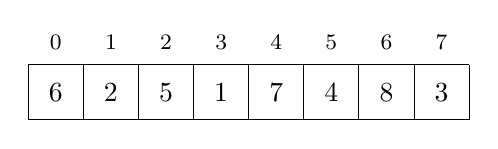
\begin{tikzpicture}[scale=0.7]
\draw (0,0) grid (8,1);
\node at (0.5,0.5) {$6$};
\node at (1.5,0.5) {$2$};
\node at (2.5,0.5) {$5$};
\node at (3.5,0.5) {$1$};
\node at (4.5,0.5) {$7$};
\node at (5.5,0.5) {$4$};
\node at (6.5,0.5) {$8$};
\node at (7.5,0.5) {$3$};

\footnotesize
\node at (0.5,1.4) {$0$};
\node at (1.5,1.4) {$1$};
\node at (2.5,1.4) {$2$};
\node at (3.5,1.4) {$3$};
\node at (4.5,1.4) {$4$};
\node at (5.5,1.4) {$5$};
\node at (6.5,1.4) {$6$};
\node at (7.5,1.4) {$7$};
\end{tikzpicture}
\end{center}
la subsecuencia creciente más larga
contiene 4 elementos:
\begin{center}
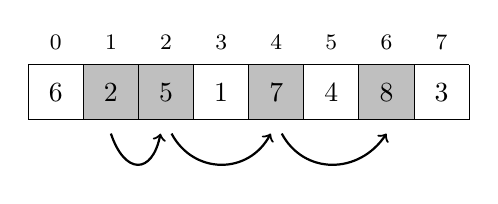
\begin{tikzpicture}[scale=0.7]
\fill[color=lightgray] (1,0) rectangle (2,1);
\fill[color=lightgray] (2,0) rectangle (3,1);
\fill[color=lightgray] (4,0) rectangle (5,1);
\fill[color=lightgray] (6,0) rectangle (7,1);
\draw (0,0) grid (8,1);
\node at (0.5,0.5) {$6$};
\node at (1.5,0.5) {$2$};
\node at (2.5,0.5) {$5$};
\node at (3.5,0.5) {$1$};
\node at (4.5,0.5) {$7$};
\node at (5.5,0.5) {$4$};
\node at (6.5,0.5) {$8$};
\node at (7.5,0.5) {$3$};

\draw[thick,->] (1.5,-0.25) .. controls (1.75,-1.00) and (2.25,-1.00) .. (2.4,-0.25);
\draw[thick,->] (2.6,-0.25) .. controls (3.0,-1.00) and (4.0,-1.00) .. (4.4,-0.25);
\draw[thick,->] (4.6,-0.25) .. controls (5.0,-1.00) and (6.0,-1.00) .. (6.5,-0.25);

\footnotesize
\node at (0.5,1.4) {$0$};
\node at (1.5,1.4) {$1$};
\node at (2.5,1.4) {$2$};
\node at (3.5,1.4) {$3$};
\node at (4.5,1.4) {$4$};
\node at (5.5,1.4) {$5$};
\node at (6.5,1.4) {$6$};
\node at (7.5,1.4) {$7$};
\end{tikzpicture}
\end{center}

Denotemos $\texttt{largo}(k)$ como
el largo de la
subsecuencia creciente más larga
que termina en la posición $k$.
Así, si calculamos todos los valores de
$\texttt{largo}(k)$ donde $0 \le k \le n-1$,
descubriremos el largo de la
subsecuencia creciente más larga.
Por ejemplo, los valores de la función
para el arreglo anterior son los siguientes:
\[
\begin{array}{lcl}
\texttt{largo}(0) & = & 1 \\
\texttt{largo}(1) & = & 1 \\
\texttt{largo}(2) & = & 2 \\
\texttt{largo}(3) & = & 1 \\
\texttt{largo}(4) & = & 3 \\
\texttt{largo}(5) & = & 2 \\
\texttt{largo}(6) & = & 4 \\
\texttt{largo}(7) & = & 2 \\
\end{array}
\]

Por ejemplo, $\texttt{largo}(6)=4$,
porque la subsecuencia creciente más larga
que termina en la posición 6 consta de 4 elementos.

Para calcular un valor de $\texttt{largo}(k)$,
debemos encontrar una posición $i<k$
tal que $\texttt{arreglo}[i]<\texttt{arreglo}[k]$
y $\texttt{largo}(i)$ sea lo más grande posible.
Entonces sabemos que
$\texttt{largo}(k)=\texttt{largo}(i)+1$,
porque esta es una forma óptima de agregar
$\texttt{arreglo}[k]$ a una subsecuencia.
Sin embargo, si no existe tal posición $i$,
entonces $\texttt{largo}(k)=1$,
lo que significa que la subsecuencia solo contiene
$\texttt{arreglo}[k]$.

Dado que todos los valores de la función se pueden calcular
a partir de sus valores más pequeños,
podemos utilizar la programación dinámica.
En el siguiente código, los valores
de la función se almacenarán en un arreglo
$\texttt{largo}$.

\begin{lstlisting}
for (int k = 0; k < n; k++) {
    largo[k] = 1;
    for (int i = 0; i < k; i++) {
        if (arreglo[i] < arreglo[k]) {
            largo[k] = max(largo[k],largo[i]+1);
        }
    }
}
\end{lstlisting}

Este código funciona en tiempo $O(n^2)$,
porque consta de dos bucles anidados.
Sin embargo, también es posible implementar
el cálculo de programación dinámica
de manera más eficiente en tiempo $O(n \log n)$.
¿Puedes encontrar una forma de hacer esto?

\section{Caminos en una cuadrícula}

Nuestro siguiente problema es encontrar un camino
desde la esquina superior izquierda hasta
la esquina inferior derecha
de una cuadrícula de $n \times n$, de tal manera que
sólo nos movemos hacia abajo y hacia la derecha.
Cada cuadro contiene un número entero positivo,
y el camino debe construirse de tal manera que
la suma de los valores a lo largo
del camino sea lo más grande posible.

La siguiente imagen muestra un camino óptimo
en una cuadrícula:
\begin{center}
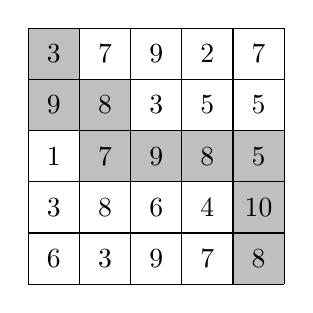
\begin{tikzpicture}[scale=.65]
  \begin{scope}
    \fill [color=lightgray] (0, 9) rectangle (1, 8);
    \fill [color=lightgray] (0, 8) rectangle (1, 7);
    \fill [color=lightgray] (1, 8) rectangle (2, 7);
    \fill [color=lightgray] (1, 7) rectangle (2, 6);
    \fill [color=lightgray] (2, 7) rectangle (3, 6);
    \fill [color=lightgray] (3, 7) rectangle (4, 6);
    \fill [color=lightgray] (4, 7) rectangle (5, 6);
    \fill [color=lightgray] (4, 6) rectangle (5, 5);
    \fill [color=lightgray] (4, 5) rectangle (5, 4);
    \draw (0, 4) grid (5, 9);
    \node at (0.5,8.5) {3};
    \node at (1.5,8.5) {7};
    \node at (2.5,8.5) {9};
    \node at (3.5,8.5) {2};
    \node at (4.5,8.5) {7};
    \node at (0.5,7.5) {9};
    \node at (1.5,7.5) {8};
    \node at (2.5,7.5) {3};
    \node at (3.5,7.5) {5};
    \node at (4.5,7.5) {5};
    \node at (0.5,6.5) {1};
    \node at (1.5,6.5) {7};
    \node at (2.5,6.5) {9};
    \node at (3.5,6.5) {8};
    \node at (4.5,6.5) {5};
    \node at (0.5,5.5) {3};
    \node at (1.5,5.5) {8};
    \node at (2.5,5.5) {6};
    \node at (3.5,5.5) {4};
    \node at (4.5,5.5) {10};
    \node at (0.5,4.5) {6};
    \node at (1.5,4.5) {3};
    \node at (2.5,4.5) {9};
    \node at (3.5,4.5) {7};
    \node at (4.5,4.5) {8};
  \end{scope}
\end{tikzpicture}
\end{center}
La suma de los valores en el camino es 67,
y esta es la suma más grande posible en un camino
desde la esquina
superior izquierda hasta la esquina inferior derecha.

Suponga que las filas y columnas de la
cuadrícula están numeradas del 1 al $n$,
y $\texttt{valor}[y][x]$ es igual al valor
del cuadro $(y,x)$.
Sea $\texttt{suma}(y,x)$ la suma máxima
en un camino desde la esquina superior izquierda
hasta el cuadro $(y,x)$.
Ahora, $\texttt{suma}(n,n)$ nos indica
la suma máxima
desde la esquina superior izquierda hasta
la esquina inferior derecha.
Por ejemplo, en la cuadrícula anterior,
$\texttt{suma}(5,5)=67$.

Podemos calcular recursivamente las sumas
de la siguiente manera:
\[ \texttt{suma}(y,x) = \max(\texttt{suma}(y,x-1),\texttt{suma}(y-1,x))+\texttt{valor}[y][x]\]

La fórmula recursiva se basa en la observación
de que un camino que termina en el cuadro $(y,x)$
puede provenir del cuadro $(y,x-1)$
o del cuadro $(y-1,x)$:
\begin{center}
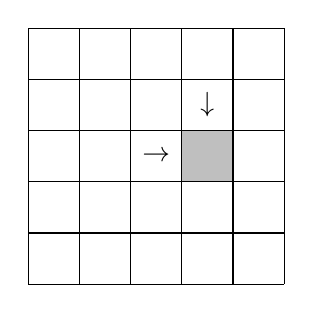
\begin{tikzpicture}[scale=.65]
  \begin{scope}
    \fill [color=lightgray] (3, 7) rectangle (4, 6);
    \draw (0, 4) grid (5, 9);
    
    \node at (2.5,6.5) {$\rightarrow$};
    \node at (3.5,7.5) {$\downarrow$};
    
  \end{scope}
\end{tikzpicture}
\end{center}

Por lo tanto, seleccionamos la dirección que maximiza
la suma.
Asumimos que $\texttt{suma}(y,x)=0$
si $y=0$ o $x=0$ (porque no existen tales caminos),
así que la fórmula recursiva también funciona cuando $y=1$ o $x=1$.

Dado que la función \texttt{suma} tiene dos parámetros,
el array de programación dinámica también tiene dos dimensiones.
Por ejemplo, podemos usar un array
\begin{lstlisting}
int suma[N][N];
\end{lstlisting}
y calcular la suma como sigue:
\begin{lstlisting}
for (int y = 1; y <= n; y++) {
    for (int x = 1; x <= n; x++) {
        suma[y][x] = max(suma[y][x-1],suma[y-1][x])+valor[y][x];
    }
}
\end{lstlisting}
La complejidad temporal del algoritmo es $O(n^2)$.

\section{Problemas de la mochila}

\index{mochila}

El término \key{mochila} se refiere a problemas donde
se da un conjunto de objetos y
se deben encontrar subconjuntos con ciertas propiedades.
Los problemas de la mochila a menudo se pueden resolver
usando programación dinámica.

En esta sección, nos enfocamos en el siguiente
problema: Dada una lista de pesos
$[w_1,w_2,\ldots,w_n]$,
determine todas
las sumas que se pueden construir usando los pesos.
Por ejemplo, si los pesos son
$[1,3,3,5]$, las siguientes sumas son posibles:

\begin{center}
\begin{tabular}{rrrrrrrrrrrrr}
 0 & 1 & 2 & 3 & 4 & 5 & 6 & 7 & 8 & 9 & 10 & 11 & 12 \\
\hline
 X & X & & X & X & X & X & X & X & X & & X & X \\
\end{tabular}
\end{center}

En este caso, todas las sumas entre $0 \ldots 12$
son posibles, excepto 2 y 10.
Por ejemplo, la suma 7 es posible porque podemos
seleccionar los pesos $[1,3,3]$.

Para resolver el problema, nos enfocamos en subproblemas
donde solo usamos los primeros $k$ pesos
para construir sumas.
Sea $\texttt{posible}(x,k)=\textrm{verdadero}$ si
podemos construir una suma $x$
usando los primeros $k$ pesos,
y de lo contrario $\texttt{posible}(x,k)=\textrm{falso}$.
Los valores de la función se pueden calcular recursivamente de la siguiente manera:
\[ \texttt{posible}(x,k) = \texttt{posible}(x-w_k,k-1) \lor \texttt{posible}(x,k-1) \]
La fórmula se basa en el hecho de que podemos
usar o no usar el peso $w_k$ en la suma.
Si usamos $w_k$, la tarea restante es formar
la suma $x-w_k$ usando los primeros $k-1$ pesos,
y si no usamos $w_k$,
la tarea restante es formar la suma $x$
usando los primeros $k-1$ pesos.
Como casos base,
\begin{equation*}
    \texttt{posible}(x,0) = \begin{cases}
               \textrm{verdadero}    & x = 0\\
               \textrm{falso}   & x \neq 0 \\
           \end{cases}
\end{equation*}
porque si no se usan pesos,
solo podemos formar la suma 0.

La siguiente tabla muestra todos los valores de la función
para los pesos $[1,3,3,5]$ (el símbolo "X"
indica los valores verdaderos):

\begin{center}
\begin{tabular}{r|rrrrrrrrrrrrr}
$k \backslash x$ & 0 & 1 & 2 & 3 & 4 & 5 & 6 & 7 & 8 & 9 & 10 & 11 & 12 \\
\hline
 0 & X & \\
 1 & X & X \\
 2 & X & X & & X & X \\
 3 & X & X & & X & X & & X & X \\
 4 & X & X & & X & X & X & X & X & X & X & & X & X \\
\end{tabular}
\end{center}

Después de calcular esos valores, $\texttt{posible}(x,n)$
nos indica si podemos construir una
suma $x$ utilizando \emph{todos} los pesos.

Denotemos $W$ como la suma total de los pesos.
La siguiente solución de programación dinámica $O(nW)$
corresponde a la función recursiva:
\begin{lstlisting}
posible[0][0] = true;
for (int k = 1; k <= n; k++) {
    for (int x = 0; x <= W; x++) {
        if (x-w[k] >= 0) posible[x][k] |= posible[x-w[k]][k-1];
        posible[x][k] |= posible[x][k-1];
    }
}
\end{lstlisting}

Sin embargo, aquí hay una mejor implementación que solo utiliza
un arreglo unidimensional $\texttt{posible}[x]$
que indica si podemos construir un subconjunto con suma $x$.
El truco es actualizar el arreglo de derecha a izquierda para
cada nuevo peso:
\begin{lstlisting}
posible[0] = true;
for (int k = 1; k <= n; k++) {
    for (int x = W; x >= 0; x--) {
        if (posible[x]) posible[x+w[k]] = true;
    }
}
\end{lstlisting}

Tenga en cuenta que la idea general presentada aquí se puede utilizar
en muchos problemas de mochila.
Por ejemplo, si se nos dan objetos con pesos y valores,
podemos determinar para cada suma de pesos el valor máximo
suma de un subconjunto.

\section{Distancia de edición}

\index{distancia de edición}
\index{distancia de Levenshtein}

La \key{distancia de edición} o \key{distancia de Levenshtein}\footnote{La distancia
lleva el nombre de V. I. Levenshtein, quien la estudió en relación con los códigos binarios \cite{lev66}.}
es el número mínimo de operaciones de edición
necesarias para transformar una cadena
en otra cadena.
Las operaciones de edición permitidas son las siguientes:
\begin{itemize}
\item insertar un carácter (por ejemplo, \texttt{ABC} $\rightarrow$ \texttt{ABCA})
\item eliminar un carácter (por ejemplo, \texttt{ABC} $\rightarrow$ \texttt{AC})
\item modificar un carácter (por ejemplo, \texttt{ABC} $\rightarrow$ \texttt{ADC})
\end{itemize}

Por ejemplo, la distancia de edición entre
\texttt{LOVE} y \texttt{MOVIE} es 2,
porque primero podemos realizar la operación
 \texttt{LOVE} $\rightarrow$ \texttt{MOVE}
(modificar) y luego la operación
\texttt{MOVE} $\rightarrow$ \texttt{MOVIE}
(insertar).
Este es el número mínimo posible de operaciones,
porque está claro que una sola operación no es suficiente.

Supongamos que se nos da una cadena \texttt{x}
de longitud $n$ y una cadena \texttt{y} de longitud $m$,
y queremos calcular la distancia de edición entre
\texttt{x} y \texttt{y}.
Para resolver el problema, definimos una función
$\texttt{distancia}(a,b)$ que proporciona la
distancia de edición entre los prefijos
$\texttt{x}[0 \ldots a]$ y $\texttt{y}[0 \ldots b]$.
Por lo tanto, usando esta función, la distancia de edición
entre \texttt{x} y \texttt{y} es igual a $\texttt{distancia}(n-1,m-1)$.

Podemos calcular los valores de \texttt{distancia}
de la siguiente manera:
\begin{equation*}
\begin{split}
\texttt{distancia}(a,b) = \min(& \texttt{distancia}(a,b-1)+1, \\
                           & \texttt{distancia}(a-1,b)+1, \\
                           & \texttt{distancia}(a-1,b-1)+\texttt{costo}(a,b)).
\end{split}
\end{equation*}
Aquí $\texttt{costo}(a,b)=0$ si $\texttt{x}[a]=\texttt{y}[b]$,
y en caso contrario $\texttt{costo}(a,b)=1$.
La fórmula considera las siguientes formas de
editar la cadena \texttt{x}:
\begin{itemize}
\item $\texttt{distancia}(a,b-1)$: insertar un carácter al final de \texttt{x}
\item $\texttt{distancia}(a-1,b)$: eliminar el último carácter de \texttt{x}
\item $\texttt{distancia}(a-1,b-1)$: coincidir o modificar el último carácter de \texttt{x}
\end{itemize}
En los dos primeros casos, se necesita una operación de edición
(insertar o eliminar).
En el último caso, si $\texttt{x}[a]=\texttt{y}[b]$,
podemos coincidir los últimos caracteres sin editar,
y en caso contrario se necesita una operación de edición (modificar).

La siguiente tabla muestra los valores de \texttt{distancia}
en el caso de ejemplo:
\begin{center}
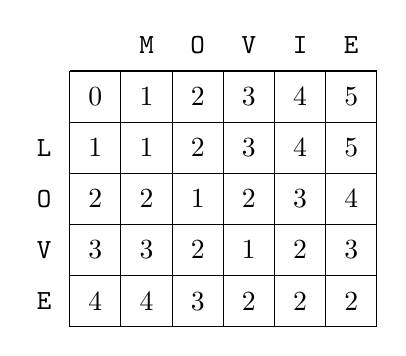
\begin{tikzpicture}[scale=.65]
  \begin{scope}
    %\fill [color=lightgray] (5, -3) rectangle (6, -4);
    \draw (1, -1) grid (7, -6);
    
    \node at (0.5,-2.5) {\texttt{L}};
    \node at (0.5,-3.5) {\texttt{O}};
    \node at (0.5,-4.5) {\texttt{V}};
    \node at (0.5,-5.5) {\texttt{E}};

    \node at (2.5,-0.5) {\texttt{M}};
    \node at (3.5,-0.5) {\texttt{O}};
    \node at (4.5,-0.5) {\texttt{V}};
    \node at (5.5,-0.5) {\texttt{I}};
    \node at (6.5,-0.5) {\texttt{E}};

    \node at (1.5,-1.5) {$0$};
    \node at (1.5,-2.5) {$1$};
    \node at (1.5,-3.5) {$2$};
    \node at (1.5,-4.5) {$3$};
    \node at (1.5,-5.5) {$4$};
    \node at (2.5,-1.5) {$1$};
    \node at (2.5,-2.5) {$1$};
    \node at (2.5,-3.5) {$2$};
    \node at (2.5,-4.5) {$3$};
    \node at (2.5,-5.5) {$4$};
    \node at (3.5,-1.5) {$2$};
    \node at (3.5,-2.5) {$2$};
    \node at (3.5,-3.5) {$1$};
    \node at (3.5,-4.5) {$2$};
    \node at (3.5,-5.5) {$3$};
    \node at (4.5,-1.5) {$3$};
    \node at (4.5,-2.5) {$3$};
    \node at (4.5,-3.5) {$2$};
    \node at (4.5,-4.5) {$1$};
    \node at (4.5,-5.5) {$2$};
    \node at (5.5,-1.5) {$4$};
    \node at (5.5,-2.5) {$4$};
    \node at (5.5,-3.5) {$3$};
    \node at (5.5,-4.5) {$2$};
    \node at (5.5,-5.5) {$2$};
    \node at (6.5,-1.5) {$5$};
    \node at (6.5,-2.5) {$5$};
    \node at (6.5,-3.5) {$4$};
    \node at (6.5,-4.5) {$3$};
    \node at (6.5,-5.5) {$2$};
  \end{scope}
\end{tikzpicture}
\end{center}

La esquina inferior derecha de la tabla
nos indica que la distancia de edición entre
\texttt{LOVE} y \texttt{MOVIE} es 2.
La tabla también muestra cómo construir
la secuencia más corta de operaciones de edición.
En este caso, el camino es el siguiente:

\begin{center}
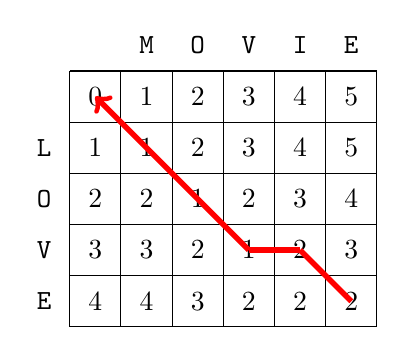
\begin{tikzpicture}[scale=.65]
  \begin{scope}
    \draw (1, -1) grid (7, -6);
    
    \node at (0.5,-2.5) {\texttt{L}};
    \node at (0.5,-3.5) {\texttt{O}};
    \node at (0.5,-4.5) {\texttt{V}};
    \node at (0.5,-5.5) {\texttt{E}};

    \node at (2.5,-0.5) {\texttt{M}};
    \node at (3.5,-0.5) {\texttt{O}};
    \node at (4.5,-0.5) {\texttt{V}};
    \node at (5.5,-0.5) {\texttt{I}};
    \node at (6.5,-0.5) {\texttt{E}};

    \node at (1.5,-1.5) {$0$};
    \node at (1.5,-2.5) {$1$};
    \node at (1.5,-3.5) {$2$};
    \node at (1.5,-4.5) {$3$};
    \node at (1.5,-5.5) {$4$};
    \node at (2.5,-1.5) {$1$};
    \node at (2.5,-2.5) {$1$};
    \node at (2.5,-3.5) {$2$};
    \node at (2.5,-4.5) {$3$};
    \node at (2.5,-5.5) {$4$};
    \node at (3.5,-1.5) {$2$};
    \node at (3.5,-2.5) {$2$};
    \node at (3.5,-3.5) {$1$};
    \node at (3.5,-4.5) {$2$};
    \node at (3.5,-5.5) {$3$};
    \node at (4.5,-1.5) {$3$};
    \node at (4.5,-2.5) {$3$};
    \node at (4.5,-3.5) {$2$};
    \node at (4.5,-4.5) {$1$};
    \node at (4.5,-5.5) {$2$};
    \node at (5.5,-1.5) {$4$};
    \node at (5.5,-2.5) {$4$};
    \node at (5.5,-3.5) {$3$};
    \node at (5.5,-4.5) {$2$};
    \node at (5.5,-5.5) {$2$};
    \node at (6.5,-1.5) {$5$};
    \node at (6.5,-2.5) {$5$};
    \node at (6.5,-3.5) {$4$};
    \node at (6.5,-4.5) {$3$};
    \node at (6.5,-5.5) {$2$};

    \path[draw=red,thick,-,line width=2pt] (6.5,-5.5) -- (5.5,-4.5);
    \path[draw=red,thick,-,line width=2pt] (5.5,-4.5) -- (4.5,-4.5);
    \path[draw=red,thick,->,line width=2pt] (4.5,-4.5) -- (1.5,-1.5);
  \end{scope}
\end{tikzpicture}
\end{center}

Los últimos caracteres de \texttt{LOVE} y \texttt{MOVIE}
son iguales, por lo que la distancia de edición entre ellos
es igual a la distancia de edición entre \texttt{LOV} y \texttt{MOVI}.
Podemos usar una operación de edición para eliminar el
carácter \texttt{I} de \texttt{MOVI}.
Por lo tanto, la distancia de edición es una unidad mayor que
la distancia de edición entre \texttt{LOV} y \texttt{MOV}, etc.

\section{Counting tilings}

Sometimes the states of a dynamic programming solution
are more complex than fixed combinations of numbers.
As an example,
consider the problem of calculating
the number of distinct ways to
fill an $n \times m$ grid using
$1 \times 2$ and $2 \times 1$ size tiles.
For example, one valid solution
for the $4 \times 7$ grid is
\begin{center}
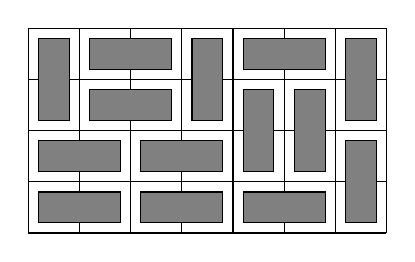
\begin{tikzpicture}[scale=.65]
    \draw (0,0) grid (7,4);
    \draw[fill=gray] (0+0.2,0+0.2) rectangle (2-0.2,1-0.2);
    \draw[fill=gray] (2+0.2,0+0.2) rectangle (4-0.2,1-0.2);
    \draw[fill=gray] (4+0.2,0+0.2) rectangle (6-0.2,1-0.2);
    \draw[fill=gray] (0+0.2,1+0.2) rectangle (2-0.2,2-0.2);
    \draw[fill=gray] (2+0.2,1+0.2) rectangle (4-0.2,2-0.2);
    \draw[fill=gray] (1+0.2,2+0.2) rectangle (3-0.2,3-0.2);
    \draw[fill=gray] (1+0.2,3+0.2) rectangle (3-0.2,4-0.2);
    \draw[fill=gray] (4+0.2,3+0.2) rectangle (6-0.2,4-0.2);

    \draw[fill=gray] (0+0.2,2+0.2) rectangle (1-0.2,4-0.2);
    \draw[fill=gray] (3+0.2,2+0.2) rectangle (4-0.2,4-0.2);
    \draw[fill=gray] (6+0.2,2+0.2) rectangle (7-0.2,4-0.2);
    \draw[fill=gray] (4+0.2,1+0.2) rectangle (5-0.2,3-0.2);
    \draw[fill=gray] (5+0.2,1+0.2) rectangle (6-0.2,3-0.2);
    \draw[fill=gray] (6+0.2,0+0.2) rectangle (7-0.2,2-0.2);

\end{tikzpicture}
\end{center}
and the total number of solutions is 781.

The problem can be solved using dynamic programming
by going through the grid row by row.
Each row in a solution can be represented as a
string that contains $m$ characters from the set
$\{\sqcap, \sqcup, \sqsubset, \sqsupset \}$.
For example, the above solution consists of four rows
that correspond to the following strings:
\begin{itemize}
\item
$\sqcap \sqsubset \sqsupset \sqcap \sqsubset \sqsupset \sqcap$
\item
$\sqcup \sqsubset \sqsupset \sqcup \sqcap \sqcap \sqcup$
\item
$\sqsubset \sqsupset \sqsubset \sqsupset \sqcup \sqcup \sqcap$ 
\item
$\sqsubset \sqsupset \sqsubset \sqsupset \sqsubset \sqsupset \sqcup$
\end{itemize}

Let $\texttt{count}(k,x)$ denote the number of ways to
construct a solution for rows $1 \ldots k$
of the grid such that string $x$ corresponds to row $k$.
It is possible to use dynamic programming here,
because the state of a row is constrained
only by the state of the previous row.

A solution is valid if row $1$ does not contain
the character $\sqcup$,
row $n$ does not contain the character $\sqcap$,
and all consecutive rows are \emph{compatible}.
For example, the rows
$\sqcup \sqsubset \sqsupset \sqcup \sqcap \sqcap \sqcup$ and
$\sqsubset \sqsupset \sqsubset \sqsupset \sqcup \sqcup \sqcap$ 
are compatible, while the rows
$\sqcap \sqsubset \sqsupset \sqcap \sqsubset \sqsupset \sqcap$ and
$\sqsubset \sqsupset \sqsubset \sqsupset \sqsubset \sqsupset \sqcup$
are not compatible.

Since a row consists of $m$ characters and there are
four choices for each character, the number of distinct
rows is at most $4^m$.
Thus, the time complexity of the solution is
$O(n 4^{2m})$ because we can go through the
$O(4^m)$ possible states for each row,
and for each state, there are $O(4^m)$
possible states for the previous row.
In practice, it is a good idea to rotate the grid
so that the shorter side has length $m$,
because the factor $4^{2m}$ dominates the time complexity.

It is possible to make the solution more efficient
by using a more compact representation for the rows.
It turns out that it is sufficient to know which
columns of the previous row contain the upper square
of a vertical tile.
Thus, we can represent a row using only characters
$\sqcap$ and $\Box$, where $\Box$ is a combination
of characters
$\sqcup$, $\sqsubset$ and $\sqsupset$.
Using this representation, there are only
$2^m$ distinct rows and the time complexity is
$O(n 2^{2m})$.

As a final note, there is also a surprising direct formula
for calculating the number of tilings\footnote{Surprisingly,
this formula was discovered in 1961 by two research teams \cite{kas61,tem61}
that worked independently.}:
\[ \prod_{a=1}^{\lceil n/2 \rceil} \prod_{b=1}^{\lceil m/2 \rceil} 4 \cdot (\cos^2 \frac{\pi a}{n + 1} + \cos^2 \frac{\pi b}{m+1})\]
This formula is very efficient, because it calculates
the number of tilings in $O(nm)$ time,
but since the answer is a product of real numbers,
a problem when using the formula is
how to store the intermediate results accurately.



\chapter{Análisis amortizado}

\index{análisis amortizado}

La complejidad temporal de un algoritmo
a menudo es fácil de analizar
simplemente examinando la estructura
del algoritmo:
qué bucles contiene el algoritmo
y cuántas veces se realizan los bucles.
Sin embargo, a veces un análisis directo
no proporciona una imagen real de la eficiencia del algoritmo.

El \key{análisis amortizado} se puede utilizar para analizar
algoritmos que contienen operaciones cuya
complejidad temporal varía.
La idea es estimar el tiempo total utilizado en
todas estas operaciones durante la
ejecución del algoritmo, en lugar de centrarse
en operaciones individuales.

\section{Método de dos punteros}

\index{dos punteros}

En el \key{método de dos punteros},
se utilizan dos punteros para
iterar a través de los valores del arreglo.
Ambos punteros pueden moverse en una dirección solamente,
lo que garantiza que el algoritmo funcione de manera eficiente.
A continuación, discutimos dos problemas que se pueden resolver
utilizando el método de dos punteros.

\subsubsection{Suma en subarreglo}

Como primer ejemplo,
consideremos un problema en el que se nos da
un arreglo de $n$ enteros positivos
y una suma objetivo $x$,
y queremos encontrar un subarreglo cuya suma sea $x$
o informar que no existe tal subarreglo.

Por ejemplo, el arreglo
\begin{center}
    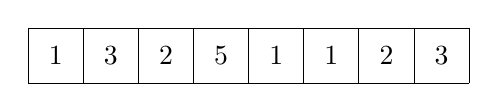
\begin{tikzpicture}[scale=0.7]
        \draw (0,0) grid (8,1);

        \node at (0.5,0.5) {$1$};
        \node at (1.5,0.5) {$3$};
        \node at (2.5,0.5) {$2$};
        \node at (3.5,0.5) {$5$};
        \node at (4.5,0.5) {$1$};
        \node at (5.5,0.5) {$1$};
        \node at (6.5,0.5) {$2$};
        \node at (7.5,0.5) {$3$};
    \end{tikzpicture}
\end{center}
contiene un subarreglo cuya suma es 8:
\begin{center}
    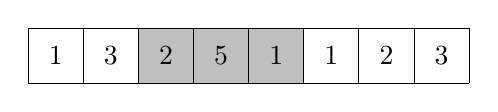
\begin{tikzpicture}[scale=0.7]
        \fill[color=lightgray] (2,0) rectangle (5,1);
        \draw (0,0) grid (8,1);

        \node at (0.5,0.5) {$1$};
        \node at (1.5,0.5) {$3$};
        \node at (2.5,0.5) {$2$};
        \node at (3.5,0.5) {$5$};
        \node at (4.5,0.5) {$1$};
        \node at (5.5,0.5) {$1$};
        \node at (6.5,0.5) {$2$};
        \node at (7.5,0.5) {$3$};
    \end{tikzpicture}
\end{center}

Este problema se puede resolver en tiempo
$O(n)$ utilizando el método de dos punteros.
La idea es mantener punteros que apuntan al
primer y último valor de un subarreglo.
En cada turno, el puntero izquierdo se mueve un paso
a la derecha, y el puntero derecho se mueve a la derecha
siempre que la suma del subarreglo resultante sea como máximo $x$.
Si la suma se convierte exactamente en $x$,
se ha encontrado una solución.

Por ejemplo, considera el siguiente arreglo
y una suma objetivo $x=8$:
\begin{center}
    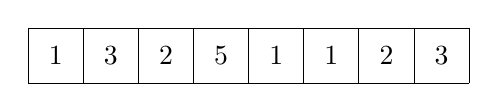
\begin{tikzpicture}[scale=0.7]
        \draw (0,0) grid (8,1);

        \node at (0.5,0.5) {$1$};
        \node at (1.5,0.5) {$3$};
        \node at (2.5,0.5) {$2$};
        \node at (3.5,0.5) {$5$};
        \node at (4.5,0.5) {$1$};
        \node at (5.5,0.5) {$1$};
        \node at (6.5,0.5) {$2$};
        \node at (7.5,0.5) {$3$};
    \end{tikzpicture}
\end{center}

El subarreglo inicial contiene los valores
1, 3 y 2 cuya suma es 6:

\begin{center}
    \begin{tikzpicture}[scale=0.7]
        \fill[color=lightgray] (0,0) rectangle (3,1);
        \draw (0,0) grid (8,1);

        \node at (0.5,0.5) {$1$};
        \node at (1.5,0.5) {$3$};
        \node at (2.5,0.5) {$2$};
        \node at (3.5,0.5) {$5$};
        \node at (4.5,0.5) {$1$};
        \node at (5.5,0.5) {$1$};
        \node at (6.5,0.5) {$2$};
        \node at (7.5,0.5) {$3$};

        \draw[thick,->] (0.5,-0.7) -- (0.5,-0.1);
        \draw[thick,->] (2.5,-0.7) -- (2.5,-0.1);
    \end{tikzpicture}
\end{center}

Luego, el puntero izquierdo se mueve un paso a la derecha.
El puntero derecho no se mueve, porque de lo contrario
la suma del subarreglo excedería $x$.

\begin{center}
    \begin{tikzpicture}[scale=0.7]
        \fill[color=lightgray] (1,0) rectangle (3,1);
        \draw (0,0) grid (8,1);

        \node at (0.5,0.5) {$1$};
        \node at (1.5,0.5) {$3$};
        \node at (2.5,0.5) {$2$};
        \node at (3.5,0.5) {$5$};
        \node at (4.5,0.5) {$1$};
        \node at (5.5,0.5) {$1$};
        \node at (6.5,0.5) {$2$};
        \node at (7.5,0.5) {$3$};

        \draw[thick,->] (1.5,-0.7) -- (1.5,-0.1);
        \draw[thick,->] (2.5,-0.7) -- (2.5,-0.1);
    \end{tikzpicture}
\end{center}

De nuevo, el puntero izquierdo se mueve un paso a la derecha,
y esta vez el puntero derecho se mueve tres
pasos a la derecha.
La suma del subarreglo es $2+5+1=8$, entonces se ha encontrado un subarreglo
cuya suma es $x$.

\begin{center}
    \begin{tikzpicture}[scale=0.7]
        \fill[color=lightgray] (2,0) rectangle (5,1);
        \draw (0,0) grid (8,1);

        \node at (0.5,0.5) {$1$};
        \node at (1.5,0.5) {$3$};
        \node at (2.5,0.5) {$2$};
        \node at (3.5,0.5) {$5$};
        \node at (4.5,0.5) {$1$};
        \node at (5.5,0.5) {$1$};
        \node at (6.5,0.5) {$2$};
        \node at (7.5,0.5) {$3$};

        \draw[thick,->] (2.5,-0.7) -- (2.5,-0.1);
        \draw[thick,->] (4.5,-0.7) -- (4.5,-0.1);
    \end{tikzpicture}
\end{center}

El tiempo de ejecución del algoritmo depende de
la cantidad de pasos que el puntero derecho se mueva.
Si bien no hay un límite superior útil sobre cuántos pasos puede
moverse el puntero en un \emph{único} turno,
sabemos que el puntero se mueve \emph{un total de}
$O(n)$ pasos durante el algoritmo,
porque solo se mueve hacia la derecha.

Dado que tanto el puntero izquierdo como el derecho
se mueven $O(n)$ pasos durante el algoritmo,
el algoritmo funciona en tiempo $O(n)$.

\subsubsection{Problema 2SUM}

Otro problema que se puede resolver usando
el método de dos punteros es el siguiente problema,
también conocido como el problema \key{2SUM}:
dado un arreglo de $n$ números y
una suma objetivo $x$, encuentre
dos valores del arreglo tales que su suma sea $x$,
o informe que no existen tales valores.

Para resolver el problema, primero
ordenamos los valores del arreglo en orden creciente.
Después de eso, iteramos a través del arreglo usando
dos punteros.
El puntero izquierdo comienza en el primer valor
y se mueve un paso a la derecha en cada turno.
El puntero derecho comienza en el último valor
y siempre se mueve hacia la izquierda hasta que la suma de los
valores izquierdo y derecho sea como máximo $x$.
Si la suma es exactamente $x$,
se ha encontrado una solución.

\pagebreak
Por ejemplo, considera el siguiente arreglo
y una suma objetivo $x=12$:
\begin{center}
    \begin{tikzpicture}[scale=0.7]
        \draw (0,0) grid (8,1);

        \node at (0.5,0.5) {$1$};
        \node at (1.5,0.5) {$4$};
        \node at (2.5,0.5) {$5$};
        \node at (3.5,0.5) {$6$};
        \node at (4.5,0.5) {$7$};
        \node at (5.5,0.5) {$9$};
        \node at (6.5,0.5) {$9$};
        \node at (7.5,0.5) {$10$};
    \end{tikzpicture}
\end{center}

Las posiciones iniciales de los punteros
son las siguientes.
La suma de los valores es $1+10=11$
que es menor que $x$.

\begin{center}
    \begin{tikzpicture}[scale=0.7]
        \fill[color=lightgray] (0,0) rectangle (1,1);
        \fill[color=lightgray] (7,0) rectangle (8,1);
        \draw (0,0) grid (8,1);

        \node at (0.5,0.5) {$1$};
        \node at (1.5,0.5) {$4$};
        \node at (2.5,0.5) {$5$};
        \node at (3.5,0.5) {$6$};
        \node at (4.5,0.5) {$7$};
        \node at (5.5,0.5) {$9$};
        \node at (6.5,0.5) {$9$};
        \node at (7.5,0.5) {$10$};

        \draw[thick,->] (0.5,-0.7) -- (0.5,-0.1);
        \draw[thick,->] (7.5,-0.7) -- (7.5,-0.1);
    \end{tikzpicture}
\end{center}

Luego, el puntero izquierdo se mueve un paso a la derecha.
El puntero derecho se mueve tres pasos a la izquierda,
y la suma se convierte en $4+7=11$.

\begin{center}
    \begin{tikzpicture}[scale=0.7]
        \fill[color=lightgray] (1,0) rectangle (2,1);
        \fill[color=lightgray] (4,0) rectangle (5,1);
        \draw (0,0) grid (8,1);

        \node at (0.5,0.5) {$1$};
        \node at (1.5,0.5) {$4$};
        \node at (2.5,0.5) {$5$};
        \node at (3.5,0.5) {$6$};
        \node at (4.5,0.5) {$7$};
        \node at (5.5,0.5) {$9$};
        \node at (6.5,0.5) {$9$};
        \node at (7.5,0.5) {$10$};

        \draw[thick,->] (1.5,-0.7) -- (1.5,-0.1);
        \draw[thick,->] (4.5,-0.7) -- (4.5,-0.1);
    \end{tikzpicture}
\end{center}

Después de esto, el puntero izquierdo se mueve un paso a la derecha nuevamente.
El puntero derecho no se mueve y se encuentra una solución
$5+7=12$.

\begin{center}
    \begin{tikzpicture}[scale=0.7]
        \fill[color=lightgray] (2,0) rectangle (3,1);
        \fill[color=lightgray] (4,0) rectangle (5,1);
        \draw (0,0) grid (8,1);

        \node at (0.5,0.5) {$1$};
        \node at (1.5,0.5) {$4$};
        \node at (2.5,0.5) {$5$};
        \node at (3.5,0.5) {$6$};
        \node at (4.5,0.5) {$7$};
        \node at (5.5,0.5) {$9$};
        \node at (6.5,0.5) {$9$};
        \node at (7.5,0.5) {$10$};

        \draw[thick,->] (2.5,-0.7) -- (2.5,-0.1);
        \draw[thick,->] (4.5,-0.7) -- (4.5,-0.1);
    \end{tikzpicture}
\end{center}

El tiempo de ejecución del algoritmo es
$O(n \log n)$, porque primero ordena
el arreglo en tiempo $O(n \log n)$,
y luego ambos punteros se mueven $O(n)$ pasos.

Ten en cuenta que es posible resolver el problema
de otra manera en tiempo $O(n \log n)$ usando búsqueda binaria.
En tal solución, iteramos a través del arreglo
y para cada valor del arreglo, intentamos encontrar otro
valor que produzca la suma $x$.
Esto se puede hacer realizando $n$ búsquedas binarias,
cada una de las cuales toma tiempo $O(\log n)$.

Un problema más difícil es
el \key{problema 3SUM}, que pide
encontrar \emph{tres} valores del arreglo
cuya suma sea $x$.
Usando la idea del algoritmo anterior,
este problema se puede resolver en tiempo $O(n^2)$.\footnote{Durante mucho tiempo,
    se pensó que resolver
    el problema 3SUM de manera más eficiente que en tiempo $O(n^2)$
    no sería posible.
    Sin embargo, en 2014, resultó \cite{gro14}
    que este no es el caso.}
¿Puedes ver cómo?

\section{Elementos menores más cercanos}

\index{elementos menores más cercanos}

El análisis amortizado se utiliza a menudo para
estimar el número de operaciones
realizadas en una estructura de datos.
Las operaciones pueden distribuirse de manera desigual de modo que
la mayoría de las operaciones ocurran durante una
fase específica del algoritmo, pero el número total
de operaciones está limitado.

Como ejemplo, considera el problema
de encontrar para cada elemento del arreglo
el \key{elemento menor más cercano}, es decir,
el primer elemento menor que precede al elemento
en el arreglo.
Es posible que no exista tal elemento,
en cuyo caso el algoritmo debe informarlo.
A continuación veremos cómo el problema puede ser
resuelto eficientemente utilizando una estructura de pila.

Recorremos el arreglo de izquierda a derecha
y mantenemos una pila de elementos del arreglo.
En cada posición del arreglo, eliminamos elementos de la pila
hasta que el elemento superior sea menor que el
elemento actual, o la pila esté vacía.
Luego, informamos que el elemento superior es
el elemento menor más cercano del elemento actual,
o si la pila está vacía, no existe tal elemento.
Finalmente, agregamos el elemento actual a la pila.

Como ejemplo, considera el siguiente arreglo:
\begin{center}
    \begin{tikzpicture}[scale=0.7]
        \draw (0,0) grid (8,1);

        \node at (0.5,0.5) {$1$};
        \node at (1.5,0.5) {$3$};
        \node at (2.5,0.5) {$4$};
        \node at (3.5,0.5) {$2$};
        \node at (4.5,0.5) {$5$};
        \node at (5.5,0.5) {$3$};
        \node at (6.5,0.5) {$4$};
        \node at (7.5,0.5) {$2$};
    \end{tikzpicture}
\end{center}

Primero, los elementos 1, 3 y 4 se agregan a la pila,
porque cada elemento es mayor que el elemento anterior.
Por lo tanto, el elemento menor más cercano de 4 es 3,
y el elemento menor más cercano de 3 es 1.
\begin{center}
    \begin{tikzpicture}[scale=0.7]
        \fill[color=lightgray] (2,0) rectangle (3,1);
        \draw (0,0) grid (8,1);

        \node at (0.5,0.5) {$1$};
        \node at (1.5,0.5) {$3$};
        \node at (2.5,0.5) {$4$};
        \node at (3.5,0.5) {$2$};
        \node at (4.5,0.5) {$5$};
        \node at (5.5,0.5) {$3$};
        \node at (6.5,0.5) {$4$};
        \node at (7.5,0.5) {$2$};

        \draw (0.2,0.2-1.2) rectangle (0.8,0.8-1.2);
        \draw (1.2,0.2-1.2) rectangle (1.8,0.8-1.2);
        \draw (2.2,0.2-1.2) rectangle (2.8,0.8-1.2);

        \node at (0.5,0.5-1.2) {$1$};
        \node at (1.5,0.5-1.2) {$3$};
        \node at (2.5,0.5-1.2) {$4$};

        \draw[->,thick] (0.8,0.5-1.2) -- (1.2,0.5-1.2);
        \draw[->,thick] (1.8,0.5-1.2) -- (2.2,0.5-1.2);
    \end{tikzpicture}
\end{center}

El siguiente elemento 2 es menor que los dos elementos superiores
en la pila.
Por lo tanto, los elementos 3 y 4 se eliminan de la pila,
y luego el elemento 2 se agrega a la pila.
Su elemento menor más cercano es 1:
\begin{center}
    \begin{tikzpicture}[scale=0.7]
        \fill[color=lightgray] (3,0) rectangle (4,1);
        \draw (0,0) grid (8,1);

        \node at (0.5,0.5) {$1$};
        \node at (1.5,0.5) {$3$};
        \node at (2.5,0.5) {$4$};
        \node at (3.5,0.5) {$2$};
        \node at (4.5,0.5) {$5$};
        \node at (5.5,0.5) {$3$};
        \node at (6.5,0.5) {$4$};
        \node at (7.5,0.5) {$2$};

        \draw (0.2,0.2-1.2) rectangle (0.8,0.8-1.2);
        \draw (3.2,0.2-1.2) rectangle (3.8,0.8-1.2);

        \node at (0.5,0.5-1.2) {$1$};
        \node at (3.5,0.5-1.2) {$2$};

        \draw[->,thick] (0.8,0.5-1.2) -- (3.2,0.5-1.2);
    \end{tikzpicture}
\end{center}

Luego, el elemento 5 es mayor que el elemento 2,
así que se agregará a la pila, y
su elemento menor más cercano es 2:
\begin{center}
    \begin{tikzpicture}[scale=0.7]
        \fill[color=lightgray] (4,0) rectangle (5,1);
        \draw (0,0) grid (8,1);

        \node at (0.5,0.5) {$1$};
        \node at (1.5,0.5) {$3$};
        \node at (2.5,0.5) {$4$};
        \node at (3.5,0.5) {$2$};
        \node at (4.5,0.5) {$5$};
        \node at (5.5,0.5) {$3$};
        \node at (6.5,0.5) {$4$};
        \node at (7.5,0.5) {$2$};

        \draw (0.2,0.2-1.2) rectangle (0.8,0.8-1.2);
        \draw (3.2,0.2-1.2) rectangle (3.8,0.8-1.2);
        \draw (4.2,0.2-1.2) rectangle (4.8,0.8-1.2);

        \node at (0.5,0.5-1.2) {$1$};
        \node at (3.5,0.5-1.2) {$2$};
        \node at (4.5,0.5-1.2) {$5$};

        \draw[->,thick] (0.8,0.5-1.2) -- (3.2,0.5-1.2);
        \draw[->,thick] (3.8,0.5-1.2) -- (4.2,0.5-1.2);
    \end{tikzpicture}
\end{center}

Después de esto, el elemento 5 se elimina de la pila
y los elementos 3 y 4 se agregan a la pila:
\begin{center}
    \begin{tikzpicture}[scale=0.7]
        \fill[color=lightgray] (6,0) rectangle (7,1);
        \draw (0,0) grid (8,1);

        \node at (0.5,0.5) {$1$};
        \node at (1.5,0.5) {$3$};
        \node at (2.5,0.5) {$4$};
        \node at (3.5,0.5) {$2$};
        \node at (4.5,0.5) {$5$};
        \node at (5.5,0.5) {$3$};
        \node at (6.5,0.5) {$4$};
        \node at (7.5,0.5) {$2$};

        \draw (0.2,0.2-1.2) rectangle (0.8,0.8-1.2);
        \draw (3.2,0.2-1.2) rectangle (3.8,0.8-1.2);
        \draw (5.2,0.2-1.2) rectangle (5.8,0.8-1.2);
        \draw (6.2,0.2-1.2) rectangle (6.8,0.8-1.2);

        \node at (0.5,0.5-1.2) {$1$};
        \node at (3.5,0.5-1.2) {$2$};
        \node at (5.5,0.5-1.2) {$3$};
        \node at (6.5,0.5-1.2) {$4$};

        \draw[->,thick] (0.8,0.5-1.2) -- (3.2,0.5-1.2);
        \draw[->,thick] (3.8,0.5-1.2) -- (5.2,0.5-1.2);
        \draw[->,thick] (5.8,0.5-1.2) -- (6.2,0.5-1.2);
    \end{tikzpicture}
\end{center}

Finalmente, todos los elementos excepto 1 son eliminados
de la pila y el último elemento 2
se agrega a la pila:

\begin{center}
    \begin{tikzpicture}[scale=0.7]
        \fill[color=lightgray] (7,0) rectangle (8,1);
        \draw (0,0) grid (8,1);

        \node at (0.5,0.5) {$1$};
        \node at (1.5,0.5) {$3$};
        \node at (2.5,0.5) {$4$};
        \node at (3.5,0.5) {$2$};
        \node at (4.5,0.5) {$5$};
        \node at (5.5,0.5) {$3$};
        \node at (6.5,0.5) {$4$};
        \node at (7.5,0.5) {$2$};

        \draw (0.2,0.2-1.2) rectangle (0.8,0.8-1.2);
        \draw (7.2,0.2-1.2) rectangle (7.8,0.8-1.2);

        \node at (0.5,0.5-1.2) {$1$};
        \node at (7.5,0.5-1.2) {$2$};

        \draw[->,thick] (0.8,0.5-1.2) -- (7.2,0.5-1.2);
    \end{tikzpicture}
\end{center}

La eficiencia del algoritmo depende del
número total de operaciones en la pila.
Si el elemento actual es más grande que
el elemento superior en la pila, se agrega directamente
a la pila, lo cual es eficiente.
Sin embargo, a veces la pila puede contener varios
elementos más grandes y lleva tiempo eliminarlos.
Aun así, cada elemento se agrega \emph{exactamente una vez} a la pila
y se elimina \emph{como máximo una vez} de la pila.
Por lo tanto, cada elemento causa $O(1)$ operaciones en la pila,
y el algoritmo funciona en tiempo $O(n)$.

\section{Mínimo en ventana deslizante}

\index{ventana deslizante}
\index{mínimo en ventana deslizante}

Una \key{ventana deslizante} es un subarreglo de tamaño constante
que se mueve de izquierda a derecha a través de un arreglo.
En cada posición de la ventana,
queremos calcular cierta información
sobre los elementos dentro de ella.
En esta sección, nos enfocamos en el problema
de mantener el \key{mínimo en ventana deslizante},
lo que significa que debemos informar el valor más
pequeño dentro de cada ventana.

El mínimo en ventana deslizante se puede calcular
usando una idea similar a la que utilizamos para calcular
los elementos menores más cercanos.
Mantenemos una cola
donde cada elemento es más grande que
el elemento anterior,
y el primer elemento
siempre corresponde al elemento mínimo dentro de la ventana.
Después de cada movimiento de ventana,
eliminamos elementos del final de la cola
hasta que el último elemento de la cola
sea más pequeño que el nuevo elemento de la ventana,
o la cola quede vacía.
También eliminamos el primer elemento de la cola
si ya no está dentro de la ventana.
Finalmente, agregamos el nuevo elemento de la ventana
al final de la cola.

Como ejemplo, considera el siguiente arreglo:

\begin{center}
    \begin{tikzpicture}[scale=0.7]
        \draw (0,0) grid (8,1);

        \node at (0.5,0.5) {$2$};
        \node at (1.5,0.5) {$1$};
        \node at (2.5,0.5) {$4$};
        \node at (3.5,0.5) {$5$};
        \node at (4.5,0.5) {$3$};
        \node at (5.5,0.5) {$4$};
        \node at (6.5,0.5) {$1$};
        \node at (7.5,0.5) {$2$};
    \end{tikzpicture}
\end{center}

Supongamos que el tamaño de la ventana deslizante es 4.
En la primera posición de la ventana, el valor más pequeño es 1:
\begin{center}
    \begin{tikzpicture}[scale=0.7]
        \fill[color=lightgray] (0,0) rectangle (4,1);
        \draw (0,0) grid (8,1);

        \node at (0.5,0.5) {$2$};
        \node at (1.5,0.5) {$1$};
        \node at (2.5,0.5) {$4$};
        \node at (3.5,0.5) {$5$};
        \node at (4.5,0.5) {$3$};
        \node at (5.5,0.5) {$4$};
        \node at (6.5,0.5) {$1$};
        \node at (7.5,0.5) {$2$};

        \draw (1.2,0.2-1.2) rectangle (1.8,0.8-1.2);
        \draw (2.2,0.2-1.2) rectangle (2.8,0.8-1.2);
        \draw (3.2,0.2-1.2) rectangle (3.8,0.8-1.2);

        \node at (1.5,0.5-1.2) {$1$};
        \node at (2.5,0.5-1.2) {$4$};
        \node at (3.5,0.5-1.2) {$5$};

        \draw[->,thick] (1.8,0.5-1.2) -- (2.2,0.5-1.2);
        \draw[->,thick] (2.8,0.5-1.2) -- (3.2,0.5-1.2);
    \end{tikzpicture}
\end{center}

Luego, la ventana se mueve un paso a la derecha.
El nuevo elemento 3 es más pequeño que los elementos
4 y 5 en la cola, por lo que los elementos 4 y 5
se eliminan de la cola
y el elemento 3 se agrega a la cola.
El valor más pequeño sigue siendo 1.
\begin{center}
    \begin{tikzpicture}[scale=0.7]
        \fill[color=lightgray] (1,0) rectangle (5,1);
        \draw (0,0) grid (8,1);

        \node at (0.5,0.5) {$2$};
        \node at (1.5,0.5) {$1$};
        \node at (2.5,0.5) {$4$};
        \node at (3.5,0.5) {$5$};
        \node at (4.5,0.5) {$3$};
        \node at (5.5,0.5) {$4$};
        \node at (6.5,0.5) {$1$};
        \node at (7.5,0.5) {$2$};

        \draw (1.2,0.2-1.2) rectangle (1.8,0.8-1.2);
        \draw (4.2,0.2-1.2) rectangle (4.8,0.8-1.2);

        \node at (1.5,0.5-1.2) {$1$};
        \node at (4.5,0.5-1.2) {$3$};

        \draw[->,thick] (1.8,0.5-1.2) -- (4.2,0.5-1.2);
    \end{tikzpicture}
\end{center}

\newpage
Después de esto, la ventana se mueve nuevamente,
y el elemento más pequeño 1
ya no pertenece a la ventana.
Por lo tanto, se elimina de la cola y ahora, el valor más pequeño
es 3. También se agrega el nuevo elemento 4
a la cola.
\begin{center}
    \begin{tikzpicture}[scale=0.7]
        \fill[color=lightgray] (2,0) rectangle (6,1);
        \draw (0,0) grid (8,1);

        \node at (0.5,0.5) {$2$};
        \node at (1.5,0.5) {$1$};
        \node at (2.5,0.5) {$4$};
        \node at (3.5,0.5) {$5$};
        \node at (4.5,0.5) {$3$};
        \node at (5.5,0.5) {$4$};
        \node at (6.5,0.5) {$1$};
        \node at (7.5,0.5) {$2$};

        \draw (4.2,0.2-1.2) rectangle (4.8,0.8-1.2);
        \draw (5.2,0.2-1.2) rectangle (5.8,0.8-1.2);

        \node at (4.5,0.5-1.2) {$3$};
        \node at (5.5,0.5-1.2) {$4$};

        \draw[->,thick] (4.8,0.5-1.2) -- (5.2,0.5-1.2);
    \end{tikzpicture}
\end{center}

El siguiente nuevo elemento 1 es más pequeño que todos los elementos
en la cola.
Por lo tanto, se eliminan todos los elementos de la cola
y solo contendrá el elemento 1:
\begin{center}
    \begin{tikzpicture}[scale=0.7]
        \fill[color=lightgray] (3,0) rectangle (7,1);
        \draw (0,0) grid (8,1);

        \node at (0.5,0.5) {$2$};
        \node at (1.5,0.5) {$1$};
        \node at (2.5,0.5) {$4$};
        \node at (3.5,0.5) {$5$};
        \node at (4.5,0.5) {$3$};
        \node at (5.5,0.5) {$4$};
        \node at (6.5,0.5) {$1$};
        \node at (7.5,0.5) {$2$};

        \draw (6.2,0.2-1.2) rectangle (6.8,0.8-1.2);

        \node at (6.5,0.5-1.2) {$1$};
    \end{tikzpicture}
\end{center}

Finalmente, la ventana llega a su última posición.
El elemento 2 se agrega a la cola,
pero el valor más pequeño dentro de la ventana
sigue siendo 1.
\begin{center}
    \begin{tikzpicture}[scale=0.7]
        \fill[color=lightgray] (4,0) rectangle (8,1);
        \draw (0,0) grid (8,1);

        \node at (0.5,0.5) {$2$};
        \node at (1.5,0.5) {$1$};
        \node at (2.5,0.5) {$4$};
        \node at (3.5,0.5) {$5$};
        \node at (4.5,0.5) {$3$};
        \node at (5.5,0.5) {$4$};
        \node at (6.5,0.5) {$1$};
        \node at (7.5,0.5) {$2$};

        \draw (6.2,0.2-1.2) rectangle (6.8,0.8-1.2);
        \draw (7.2,0.2-1.2) rectangle (7.8,0.8-1.2);

        \node at (6.5,0.5-1.2) {$1$};
        \node at (7.5,0.5-1.2) {$2$};

        \draw[->,thick] (6.8,0.5-1.2) -- (7.2,0.5-1.2);
    \end{tikzpicture}
\end{center}

Dado que cada elemento del arreglo
se agrega a la cola exactamente una vez y
se elimina de la cola como máximo una vez,
el algoritmo funciona en tiempo $O(n)$.



\chapter{Consultas en rangos}

\index{consultas en rangos}
\indexalt{preguntas en rangos}
\indexalt{queries en rangos}

En este capítulo discutiremos estructuras de datos
que nos permiten procesar consultas en rangos (\textit{range queries})
de manera eficiente. En una \key{consulta en rango},
nuestra tarea es calcular un valor
basado en un subarreglo de un arreglo.
Las consultas típicas son:
\begin{itemize}
    \item $\texttt{suma}_q(a,b)$: calcular la suma de valores en el rango $[a,b]$
    \item $\texttt{min}_q(a,b)$: encontrar el valor mínimo en el rango $[a,b]$
    \item $\texttt{max}_q(a,b)$: encontrar el valor máximo en el rango $[a,b]$
\end{itemize}

Donde la letra \textit{q} denota una consulta en el subarreglo. Por ejemplo, considera el rango $[3,6]$ en el siguiente arreglo:
\begin{center}
    \begin{tikzpicture}[scale=0.7]
        \fill[color=lightgray] (3,0) rectangle (7,1);
        \draw (0,0) grid (8,1);

        \node at (0.5,0.5) {$1$};
        \node at (1.5,0.5) {$3$};
        \node at (2.5,0.5) {$8$};
        \node at (3.5,0.5) {$4$};
        \node at (4.5,0.5) {$6$};
        \node at (5.5,0.5) {$1$};
        \node at (6.5,0.5) {$3$};
        \node at (7.5,0.5) {$4$};

        \footnotesize
        \node at (0.5,1.4) {$0$};
        \node at (1.5,1.4) {$1$};
        \node at (2.5,1.4) {$2$};
        \node at (3.5,1.4) {$3$};
        \node at (4.5,1.4) {$4$};
        \node at (5.5,1.4) {$5$};
        \node at (6.5,1.4) {$6$};
        \node at (7.5,1.4) {$7$};
    \end{tikzpicture}
\end{center}
En este caso, $\texttt{suma}_q(3,6)=14$,
$\texttt{min}_q(3,6)=1$ y $\texttt{max}_q(3,6)=6$.

Una forma simple de procesar consultas de rango es usar
un bucle que recorre todos los valores del arreglo en el rango.
Por ejemplo, podemos usar la siguiente función para procesar
consultas de suma en un arreglo:

\begin{lstlisting}
int sum(int a, int b) {
    int s = 0;
    for (int i = a; i <= b; i++) {
        s += arreglo[i];
    }
    return s;
}
\end{lstlisting}

Esta función funciona en $O(n)$,
donde $n$ es el tamaño del arreglo.
Por lo tanto, podemos procesar $q$ consultas en $O(nq)$
usando la función.
Sin embargo, si tanto $n$ como $q$ son grandes, este método
es muy lento. Afortunadamente, resulta que existen
maneras de procesar consultas de rango mucho más eficientemente.

\section{Consultas en arreglos estáticos}

Primero nos enfocaremos en una situación donde
el arreglo es \emph{estático}, es decir,
los valores del arreglo nunca se actualizan entre las consultas.
En este caso, basta con construir
una estructura de datos estática que nos indique
la respuesta para cualquier consulta posible.

\subsubsection{Consultas de suma}

\index{arreglo de sumas de prefijos}
\indexalt{suma prefija}
\indexalt{suma acumulativa}

Podemos fácilmente procesar consultas de suma en un arreglo estático
construyendo un \key{arreglo de sumas de prefijos}.
Cada valor en este arreglo equivale a la suma de valores en el
arreglo original \emph{hasta} esa posición, o sea, el valor en
cada posición $k$ es igual a $\texttt{suma}_q(0,k)$.
El arreglo de sumas de prefijos puede construirse en $O(n)$,
ya que cada valor solo depende del anterior.

Por ejemplo, considera el siguiente arreglo:

\begin{center}
    \begin{tikzpicture}[scale=0.7]
        %\fill[color=lightgray] (3,0) rectangle (7,1);
        \draw (0,0) grid (8,1);

        \node at (0.5,0.5) {$1$};
        \node at (1.5,0.5) {$3$};
        \node at (2.5,0.5) {$4$};
        \node at (3.5,0.5) {$8$};
        \node at (4.5,0.5) {$6$};
        \node at (5.5,0.5) {$1$};
        \node at (6.5,0.5) {$4$};
        \node at (7.5,0.5) {$2$};

        \footnotesize
        \node at (0.5,1.4) {$0$};
        \node at (1.5,1.4) {$1$};
        \node at (2.5,1.4) {$2$};
        \node at (3.5,1.4) {$3$};
        \node at (4.5,1.4) {$4$};
        \node at (5.5,1.4) {$5$};
        \node at (6.5,1.4) {$6$};
        \node at (7.5,1.4) {$7$};
    \end{tikzpicture}
\end{center}

Su arreglo de sumas de prefijos es el siguiente:
\begin{center}
    \begin{tikzpicture}[scale=0.7]
        \draw (0,0) grid (8,1);

        \node at (0.5,0.5) {$1$};
        \node at (1.5,0.5) {$4$};
        \node at (2.5,0.5) {$8$};
        \node at (3.5,0.5) {$16$};
        \node at (4.5,0.5) {$22$};
        \node at (5.5,0.5) {$23$};
        \node at (6.5,0.5) {$27$};
        \node at (7.5,0.5) {$29$};

        \footnotesize
        \node at (0.5,1.4) {$0$};
        \node at (1.5,1.4) {$1$};
        \node at (2.5,1.4) {$2$};
        \node at (3.5,1.4) {$3$};
        \node at (4.5,1.4) {$4$};
        \node at (5.5,1.4) {$5$};
        \node at (6.5,1.4) {$6$};
        \node at (7.5,1.4) {$7$};
    \end{tikzpicture}
\end{center}

Dado que el arreglo de sumas de prefijos contiene todo valor
de $\texttt{suma}_q(0,k)$,
podemos calcular cualquier valor de
$\texttt{suma}_q(a,b)$ en $O(1)$ de la siguiente manera:
\[ \texttt{suma}_q(a,b) = \texttt{suma}_q(0,b) - \texttt{suma}_q(0,a-1)\]
Definiendo $\texttt{suma}_q(0,-1)=0$,
la fórmula anterior también se cumple cuando $a=0$.

Por ejemplo, considera el rango $[3,6]$:
\begin{center}
    \begin{tikzpicture}[scale=0.7]
        \fill[color=lightgray] (3,0) rectangle (7,1);
        \draw (0,0) grid (8,1);

        \node at (0.5,0.5) {$1$};
        \node at (1.5,0.5) {$3$};
        \node at (2.5,0.5) {$4$};
        \node at (3.5,0.5) {$8$};
        \node at (4.5,0.5) {$6$};
        \node at (5.5,0.5) {$1$};
        \node at (6.5,0.5) {$4$};
        \node at (7.5,0.5) {$2$};

        \footnotesize
        \node at (0.5,1.4) {$0$};
        \node at (1.5,1.4) {$1$};
        \node at (2.5,1.4) {$2$};
        \node at (3.5,1.4) {$3$};
        \node at (4.5,1.4) {$4$};
        \node at (5.5,1.4) {$5$};
        \node at (6.5,1.4) {$6$};
        \node at (7.5,1.4) {$7$};
    \end{tikzpicture}
\end{center}

En este caso $\texttt{suma}_q(3,6)=8+6+1+4=19$.
Esta suma se puede calcular a partir de
dos valores del arreglo de suma de prefijos:
\begin{center}
    \begin{tikzpicture}[scale=0.7]
        \fill[color=lightgray] (2,0) rectangle (3,1);
        \fill[color=lightgray] (6,0) rectangle (7,1);
        \draw (0,0) grid (8,1);

        \node at (0.5,0.5) {$1$};
        \node at (1.5,0.5) {$4$};
        \node at (2.5,0.5) {$8$};
        \node at (3.5,0.5) {$16$};
        \node at (4.5,0.5) {$22$};
        \node at (5.5,0.5) {$23$};
        \node at (6.5,0.5) {$27$};
        \node at (7.5,0.5) {$29$};

        \footnotesize
        \node at (0.5,1.4) {$0$};
        \node at (1.5,1.4) {$1$};
        \node at (2.5,1.4) {$2$};
        \node at (3.5,1.4) {$3$};
        \node at (4.5,1.4) {$4$};
        \node at (5.5,1.4) {$5$};
        \node at (6.5,1.4) {$6$};
        \node at (7.5,1.4) {$7$};
    \end{tikzpicture}
\end{center}
Así, $\texttt{suma}_q(3,6)=\texttt{suma}_q(0,6)-\texttt{suma}_q(0,2)=27-8=19$.

También es posible generalizar esta idea
a dimensiones superiores.
Por ejemplo, podemos construir una matriz
de sumas de prefijos que se puede utilizar para calcular
la suma de cualquier subarreglo rectangular en $O(1)$.
Cada suma en dicho arreglo corresponde a
un subarreglo que comienza en la esquina superior
izquierda del arreglo.

\pagebreak
La siguiente imagen ilustra la idea:
\begin{center}
    \begin{tikzpicture}[scale=0.54]
        \draw[fill=lightgray] (3,2) rectangle (7,5);
        \draw (0,0) grid (10,7);
        \node[anchor=center] at (6.5, 2.5) {$A$};
        \node[anchor=center] at (2.5, 2.5) {$B$};
        \node[anchor=center] at (6.5, 5.5) {$C$};
        \node[anchor=center] at (2.5, 5.5) {$D$};
    \end{tikzpicture}
\end{center}

La suma del subarreglo gris se puede calcular
usando la fórmula
\[S(A) - S(B) - S(C) + S(D),\]
donde $S(X)$ denota la suma de valores
en un subarreglo rectangular
desde la esquina superior izquierda
hasta la posición de $X$.

\subsubsection{Consultas de mínimo}

\index{tabla dispersa}

Las consultas de mínimo son más difíciles de procesar
que las consultas de suma.
Sin embargo, hay un método de preprocesamiento bastante simple
en $O(n \log n)$ luego del cual podemos responder a
cualquier consulta de mínimo en $O(1)$.\footnote{Esta técnica
    fue introducida en \cite{ben00} y a veces
    se llama método de \key{tabla dispersa} (\textit{sparse table}).
    También existen técnicas más sofisticadas \cite{fis06} donde
    el tiempo de preprocesamiento es solo $O(n)$, pero tales algoritmos
    no son necesarios en programación competitiva.}
Ten en cuenta que, dado que las consultas de mínimo y máximo se pueden
procesar de manera similar, nos centraremos en las consultas de mínimo.

La idea es precalcular todos los valores de
$\textrm{min}_q(a,b)$ donde
$b-a+1$ (la longitud del rango $[a,b]$) sea una potencia de dos.
Por ejemplo, para el arreglo

\begin{center}
    \begin{tikzpicture}[scale=0.7]
        \draw (0,0) grid (8,1);

        \node at (0.5,0.5) {$1$};
        \node at (1.5,0.5) {$3$};
        \node at (2.5,0.5) {$4$};
        \node at (3.5,0.5) {$8$};
        \node at (4.5,0.5) {$6$};
        \node at (5.5,0.5) {$1$};
        \node at (6.5,0.5) {$4$};
        \node at (7.5,0.5) {$2$};

        \footnotesize
        \node at (0.5,1.4) {$0$};
        \node at (1.5,1.4) {$1$};
        \node at (2.5,1.4) {$2$};
        \node at (3.5,1.4) {$3$};
        \node at (4.5,1.4) {$4$};
        \node at (5.5,1.4) {$5$};
        \node at (6.5,1.4) {$6$};
        \node at (7.5,1.4) {$7$};
    \end{tikzpicture}
\end{center}
se calculan los siguientes valores:

\begin{center}
    \begin{tabular}{ccc}

        \begin{tabular}{lll}
            $a$ & $b$ & $\texttt{min}_q(a,b)$ \\
            \hline
            0   & 0   & 1                     \\
            1   & 1   & 3                     \\
            2   & 2   & 4                     \\
            3   & 3   & 8                     \\
            4   & 4   & 6                     \\
            5   & 5   & 1                     \\
            6   & 6   & 4                     \\
            7   & 7   & 2                     \\
        \end{tabular}

         &

        \begin{tabular}{lll}
            $a$ & $b$ & $\texttt{min}_q(a,b)$ \\
            \hline
            0   & 1   & 1                     \\
            1   & 2   & 3                     \\
            2   & 3   & 4                     \\
            3   & 4   & 6                     \\
            4   & 5   & 1                     \\
            5   & 6   & 1                     \\
            6   & 7   & 2                     \\
            \\
        \end{tabular}

         &

        \begin{tabular}{lll}
            $a$ & $b$ & $\texttt{min}_q(a,b)$ \\
            \hline
            0   & 3   & 1                     \\
            1   & 4   & 3                     \\
            2   & 5   & 1                     \\
            3   & 6   & 1                     \\
            4   & 7   & 1                     \\
            0   & 7   & 1                     \\
            \\
            \\
        \end{tabular}
    \end{tabular}
\end{center}

El número de valores precalculados es $O(n \log n)$,
porque hay $O(\log n)$ longitudes de rango
que son potencias de dos.
Los valores se pueden calcular de manera eficiente
usando la fórmula recursiva
\[\texttt{min}_q(a,b) = \min(\texttt{min}_q(a,a+w-1),\texttt{min}_q(a+w,b)),\]
donde $b-a+1$ es una potencia de dos y $w=(b-a+1)/2$.
Calcular todos esos valores toma un tiempo de $O(n \log n)$.

Después de esto, cualquier valor de $\texttt{min}_q(a,b)$ se puede calcular
en  $O(1)$ como el mínimo de dos valores precalculados.
Sea $k$ la mayor potencia de dos que no exceda $b-a+1$.
Podemos calcular el valor de $\texttt{min}_q(a,b)$ usando la fórmula
\[\texttt{min}_q(a,b) = \min(\texttt{min}_q(a,a+k-1),\texttt{min}_q(b-k+1,b)).\]
En la fórmula anterior, el rango $[a,b]$ se representa
como la unión de los rangos $[a,a+k-1]$ y $[b-k+1,b]$, ambos de longitud $k$.

Como ejemplo, considera el rango $[1,6]$:
\begin{center}
    \begin{tikzpicture}[scale=0.7]
        \fill[color=lightgray] (1,0) rectangle (7,1);
        \draw (0,0) grid (8,1);

        \node at (0.5,0.5) {$1$};
        \node at (1.5,0.5) {$3$};
        \node at (2.5,0.5) {$4$};
        \node at (3.5,0.5) {$8$};
        \node at (4.5,0.5) {$6$};
        \node at (5.5,0.5) {$1$};
        \node at (6.5,0.5) {$4$};
        \node at (7.5,0.5) {$2$};

        \footnotesize
        \node at (0.5,1.4) {$0$};
        \node at (1.5,1.4) {$1$};
        \node at (2.5,1.4) {$2$};
        \node at (3.5,1.4) {$3$};
        \node at (4.5,1.4) {$4$};
        \node at (5.5,1.4) {$5$};
        \node at (6.5,1.4) {$6$};
        \node at (7.5,1.4) {$7$};
    \end{tikzpicture}
\end{center}
La longitud del rango es 6,
y la mayor potencia de dos que no
exceda 6 es 4.
Por lo tanto, el rango $[1,6]$ es
la unión de los rangos $[1,4]$ y $[3,6]$:
\begin{center}
    \begin{tikzpicture}[scale=0.7]
        \fill[color=lightgray] (1,0) rectangle (5,1);
        \draw (0,0) grid (8,1);

        \node at (0.5,0.5) {$1$};
        \node at (1.5,0.5) {$3$};
        \node at (2.5,0.5) {$4$};
        \node at (3.5,0.5) {$8$};
        \node at (4.5,0.5) {$6$};
        \node at (5.5,0.5) {$1$};
        \node at (6.5,0.5) {$4$};
        \node at (7.5,0.5) {$2$};

        \footnotesize
        \node at (0.5,1.4) {$0$};
        \node at (1.5,1.4) {$1$};
        \node at (2.5,1.4) {$2$};
        \node at (3.5,1.4) {$3$};
        \node at (4.5,1.4) {$4$};
        \node at (5.5,1.4) {$5$};
        \node at (6.5,1.4) {$6$};
        \node at (7.5,1.4) {$7$};
    \end{tikzpicture}
\end{center}
\begin{center}
    \begin{tikzpicture}[scale=0.7]
        \fill[color=lightgray] (3,0) rectangle (7,1);
        \draw (0,0) grid (8,1);

        \node at (0.5,0.5) {$1$};
        \node at (1.5,0.5) {$3$};
        \node at (2.5,0.5) {$4$};
        \node at (3.5,0.5) {$8$};
        \node at (4.5,0.5) {$6$};
        \node at (5.5,0.5) {$1$};
        \node at (6.5,0.5) {$4$};
        \node at (7.5,0.5) {$2$};


        \footnotesize
        \node at (0.5,1.4) {$0$};
        \node at (1.5,1.4) {$1$};
        \node at (2.5,1.4) {$2$};
        \node at (3.5,1.4) {$3$};
        \node at (4.5,1.4) {$4$};
        \node at (5.5,1.4) {$5$};
        \node at (6.5,1.4) {$6$};
        \node at (7.5,1.4) {$7$};
    \end{tikzpicture}
\end{center}
Dado que $\texttt{min}_q(1,4)=3$ y $\texttt{min}_q(3,6)=1$,
concluimos que $\texttt{min}_q(1,6)=1$.


\section{Árbol binario indexado}

\index{árbol!binario indexado}
\indexaltsub{árbol}{de Fenwick}

Un \key{árbol binario indexado} o \key{árbol de Fenwick}\footnote{La
    estructura del árbol binario indexado fue presentada por P. M. Fenwick en 1994 \cite{fen94}.}
puede verse como una variante dinámica del arreglo de sumas de prefijos.
Admite dos operaciones de $O(\log n)$ en un arreglo:
procesar una consulta de suma en rango y actualizar un valor.

La ventaja de un árbol binario indexado es
que nos permite actualizar de manera eficiente
los valores del arreglo entre consultas de suma.
Esto no sería posible utilizando un arreglo de suma de prefijos,
porque después de cada actualización, sería necesario construir todo
el arreglo de suma de prefijos nuevamente en $O(n)$.

\subsubsection{Estructura}

Aunque el nombre de la estructura hace referencia a un árbol,
generalmente se representa como un arreglo.
En esta sección asumimos que todos los arreglos tienen índice base uno,
ya que facilita la implementación.

Definamos $p(k)$ como la mayor potencia de 2 que
divide a $k$.
Almacenamos un árbol binario indexado como un arreglo \texttt{árbol}
tal que
\[ \texttt{árbol}[k] = \texttt{suma}_q(k-p(k)+1,k),\]
es decir, cada posición $k$ contiene la suma de los valores
en un rango del arreglo original cuya longitud es $p(k)$
y que termina en la posición $k$.
Por ejemplo, dado que $p(6)=2$, $\texttt{arbol}[6]$
contiene el valor de $\texttt{suma}_q(5,6)$.

Por ejemplo, considera el siguiente arreglo:
\begin{center}
    \begin{tikzpicture}[scale=0.7]
        \draw (0,0) grid (8,1);

        \node at (0.5,0.5) {$1$};
        \node at (1.5,0.5) {$3$};
        \node at (2.5,0.5) {$4$};
        \node at (3.5,0.5) {$8$};
        \node at (4.5,0.5) {$6$};
        \node at (5.5,0.5) {$1$};
        \node at (6.5,0.5) {$4$};
        \node at (7.5,0.5) {$2$};

        \footnotesize
        \node at (0.5,1.4) {$1$};
        \node at (1.5,1.4) {$2$};
        \node at (2.5,1.4) {$3$};
        \node at (3.5,1.4) {$4$};
        \node at (4.5,1.4) {$5$};
        \node at (5.5,1.4) {$6$};
        \node at (6.5,1.4) {$7$};
        \node at (7.5,1.4) {$8$};
    \end{tikzpicture}
\end{center}

El árbol binario indexado correspondiente es el siguiente:
\begin{center}
    \begin{tikzpicture}[scale=0.7]
        \draw (0,0) grid (8,1);

        \node at (0.5,0.5) {$1$};
        \node at (1.5,0.5) {$4$};
        \node at (2.5,0.5) {$4$};
        \node at (3.5,0.5) {$16$};
        \node at (4.5,0.5) {$6$};
        \node at (5.5,0.5) {$7$};
        \node at (6.5,0.5) {$4$};
        \node at (7.5,0.5) {$29$};

        \footnotesize
        \node at (0.5,1.4) {$1$};
        \node at (1.5,1.4) {$2$};
        \node at (2.5,1.4) {$3$};
        \node at (3.5,1.4) {$4$};
        \node at (4.5,1.4) {$5$};
        \node at (5.5,1.4) {$6$};
        \node at (6.5,1.4) {$7$};
        \node at (7.5,1.4) {$8$};
    \end{tikzpicture}
\end{center}

La siguiente imagen muestra de manera más clara
cómo cada valor en el árbol binario indexado
corresponde a un rango en el arreglo original:

\begin{center}
    \begin{tikzpicture}[scale=0.7]
        \draw (0,0) grid (8,1);

        \node at (0.5,0.5) {$1$};
        \node at (1.5,0.5) {$4$};
        \node at (2.5,0.5) {$4$};
        \node at (3.5,0.5) {$16$};
        \node at (4.5,0.5) {$6$};
        \node at (5.5,0.5) {$7$};
        \node at (6.5,0.5) {$4$};
        \node at (7.5,0.5) {$29$};

        \footnotesize
        \node at (0.5,1.4) {$1$};
        \node at (1.5,1.4) {$2$};
        \node at (2.5,1.4) {$3$};
        \node at (3.5,1.4) {$4$};
        \node at (4.5,1.4) {$5$};
        \node at (5.5,1.4) {$6$};
        \node at (6.5,1.4) {$7$};
        \node at (7.5,1.4) {$8$};

        \draw[->,thick] (0.5,-0.9) -- (0.5,-0.1);
        \draw[->,thick] (2.5,-0.9) -- (2.5,-0.1);
        \draw[->,thick] (4.5,-0.9) -- (4.5,-0.1);
        \draw[->,thick] (6.5,-0.9) -- (6.5,-0.1);
        \draw[->,thick] (1.5,-1.9) -- (1.5,-0.1);
        \draw[->,thick] (5.5,-1.9) -- (5.5,-0.1);
        \draw[->,thick] (3.5,-2.9) -- (3.5,-0.1);
        \draw[->,thick] (7.5,-3.9) -- (7.5,-0.1);

        \draw (0,-1) -- (1,-1) -- (1,-1.5) -- (0,-1.5) -- (0,-1);
        \draw (2,-1) -- (3,-1) -- (3,-1.5) -- (2,-1.5) -- (2,-1);
        \draw (4,-1) -- (5,-1) -- (5,-1.5) -- (4,-1.5) -- (4,-1);
        \draw (6,-1) -- (7,-1) -- (7,-1.5) -- (6,-1.5) -- (6,-1);
        \draw (0,-2) -- (2,-2) -- (2,-2.5) -- (0,-2.5) -- (0,-2);
        \draw (4,-2) -- (6,-2) -- (6,-2.5) -- (4,-2.5) -- (4,-2);
        \draw (0,-3) -- (4,-3) -- (4,-3.5) -- (0,-3.5) -- (0,-3);
        \draw (0,-4) -- (8,-4) -- (8,-4.5) -- (0,-4.5) -- (0,-4);
    \end{tikzpicture}
\end{center}

Usando un árbol binario indexado,
cualquier valor de $\texttt{suma}_q(1,k)$
se puede calcular en $O(\log n)$,
porque un rango $[1,k]$ siempre se puede dividir en
$O(\log n)$ rangos cuyas sumas están almacenadas en el árbol.

Por ejemplo, el rango $[1,7]$ consta de
los siguientes rangos:
\begin{center}
    \begin{tikzpicture}[scale=0.7]
        \draw (0,0) grid (8,1);

        \node at (0.5,0.5) {$1$};
        \node at (1.5,0.5) {$4$};
        \node at (2.5,0.5) {$4$};
        \node at (3.5,0.5) {$16$};
        \node at (4.5,0.5) {$6$};
        \node at (5.5,0.5) {$7$};
        \node at (6.5,0.5) {$4$};
        \node at (7.5,0.5) {$29$};

        \footnotesize
        \node at (0.5,1.4) {$1$};
        \node at (1.5,1.4) {$2$};
        \node at (2.5,1.4) {$3$};
        \node at (3.5,1.4) {$4$};
        \node at (4.5,1.4) {$5$};
        \node at (5.5,1.4) {$6$};
        \node at (6.5,1.4) {$7$};
        \node at (7.5,1.4) {$8$};

        \draw[->,thick] (0.5,-0.9) -- (0.5,-0.1);
        \draw[->,thick] (2.5,-0.9) -- (2.5,-0.1);
        \draw[->,thick] (4.5,-0.9) -- (4.5,-0.1);
        \draw[->,thick] (6.5,-0.9) -- (6.5,-0.1);
        \draw[->,thick] (1.5,-1.9) -- (1.5,-0.1);
        \draw[->,thick] (5.5,-1.9) -- (5.5,-0.1);
        \draw[->,thick] (3.5,-2.9) -- (3.5,-0.1);
        \draw[->,thick] (7.5,-3.9) -- (7.5,-0.1);

        \draw (0,-1) -- (1,-1) -- (1,-1.5) -- (0,-1.5) -- (0,-1);
        \draw (2,-1) -- (3,-1) -- (3,-1.5) -- (2,-1.5) -- (2,-1);
        \draw (4,-1) -- (5,-1) -- (5,-1.5) -- (4,-1.5) -- (4,-1);
        \draw[fill=lightgray] (6,-1) -- (7,-1) -- (7,-1.5) -- (6,-1.5) -- (6,-1);
        \draw (0,-2) -- (2,-2) -- (2,-2.5) -- (0,-2.5) -- (0,-2);
        \draw[fill=lightgray] (4,-2) -- (6,-2) -- (6,-2.5) -- (4,-2.5) -- (4,-2);
        \draw[fill=lightgray] (0,-3) -- (4,-3) -- (4,-3.5) -- (0,-3.5) -- (0,-3);
        \draw (0,-4) -- (8,-4) -- (8,-4.5) -- (0,-4.5) -- (0,-4);
    \end{tikzpicture}
\end{center}
Por lo tanto, podemos calcular la suma correspondiente de la siguiente manera:
\[\texttt{suma}_q(1,7)=\texttt{suma}_q(1,4)+\texttt{suma}_q(5,6)+\texttt{suma}_q(7,7)=16+7+4=27\]

Para calcular el valor de $\texttt{suma}_q(a,b)$ donde $a>1$,
podemos usar el mismo truco que utilizamos con arreglos de sumas de prefijos:
\[ \texttt{suma}_q(a,b) = \texttt{suma}_q(1,b) - \texttt{suma}_q(1,a-1).\]
Dado que podemos calcular tanto $\texttt{suma}_q(1,b)$
como $\texttt{suma}_q(1,a-1)$ en $O(\log n)$,
la complejidad total del tiempo es $O(\log n)$.

Luego, después de actualizar un valor en el arreglo original,
varios valores en el árbol binario indexado
deben ser actualizados.
Por ejemplo, si el valor en la posición 3 cambia,
las sumas de los siguientes rangos cambian:
\begin{center}
    \begin{tikzpicture}[scale=0.7]
        \draw (0,0) grid (8,1);

        \node at (0.5,0.5) {$1$};
        \node at (1.5,0.5) {$4$};
        \node at (2.5,0.5) {$4$};
        \node at (3.5,0.5) {$16$};
        \node at (4.5,0.5) {$6$};
        \node at (5.5,0.5) {$7$};
        \node at (6.5,0.5) {$4$};
        \node at (7.5,0.5) {$29$};

        \footnotesize
        \node at (0.5,1.4) {$1$};
        \node at (1.5,1.4) {$2$};
        \node at (2.5,1.4) {$3$};
        \node at (3.5,1.4) {$4$};
        \node at (4.5,1.4) {$5$};
        \node at (5.5,1.4) {$6$};
        \node at (6.5,1.4) {$7$};
        \node at (7.5,1.4) {$8$};

        \draw[->,thick] (0.5,-0.9) -- (0.5,-0.1);
        \draw[->,thick] (2.5,-0.9) -- (2.5,-0.1);
        \draw[->,thick] (4.5,-0.9) -- (4.5,-0.1);
        \draw[->,thick] (6.5,-0.9) -- (6.5,-0.1);
        \draw[->,thick] (1.5,-1.9) -- (1.5,-0.1);
        \draw[->,thick] (5.5,-1.9) -- (5.5,-0.1);
        \draw[->,thick] (3.5,-2.9) -- (3.5,-0.1);
        \draw[->,thick] (7.5,-3.9) -- (7.5,-0.1);

        \draw (0,-1) -- (1,-1) -- (1,-1.5) -- (0,-1.5) -- (0,-1);
        \draw[fill=lightgray] (2,-1) -- (3,-1) -- (3,-1.5) -- (2,-1.5) -- (2,-1);
        \draw (4,-1) -- (5,-1) -- (5,-1.5) -- (4,-1.5) -- (4,-1);
        \draw (6,-1) -- (7,-1) -- (7,-1.5) -- (6,-1.5) -- (6,-1);
        \draw (0,-2) -- (2,-2) -- (2,-2.5) -- (0,-2.5) -- (0,-2);
        \draw (4,-2) -- (6,-2) -- (6,-2.5) -- (4,-2.5) -- (4,-2);
        \draw[fill=lightgray] (0,-3) -- (4,-3) -- (4,-3.5) -- (0,-3.5) -- (0,-3);
        \draw[fill=lightgray] (0,-4) -- (8,-4) -- (8,-4.5) -- (0,-4.5) -- (0,-4);
    \end{tikzpicture}
\end{center}

Dado que cada elemento del arreglo pertenece a $O(\log n)$
rangos en el árbol binario indexado,
basta con actualizar $O(\log n)$ valores en el árbol.

\subsubsection{Implementación}

Las operaciones de un árbol binario indexado pueden ser
implementadas de manera eficiente usando operaciones de bits.
El hecho clave necesario es que podemos
calcular cualquier valor de $p(k)$ usando la siguiente fórmula:
\[p(k) = k \& (-k)\]

La siguiente función calcula el valor de $\texttt{suma}_q(1,k)$:
\begin{lstlisting}
int suma(int k) {
    int s = 0;
    while (k >= 1) {
        s += árbol[k];
        k -= k & -k;
    }
    return s;
}
\end{lstlisting}

\newpage
La siguiente función aumenta el
valor del arreglo en la posición $k$ por $x$
($x$ puede ser positivo o negativo):

\begin{lstlisting}
void agregar(int k, int x) {
    while (k <= n) {
        árbol[k] += x;
        k += k & -k;
    }
}
\end{lstlisting}

La complejidad temporal de ambas funciones es
$O(\log n)$, porque las funciones acceden a $O(\log n)$
valores en el árbol binario indexado, y cada movimiento
a la siguiente posición toma $O(1)$.

\section{Árbol de segmentos}

\index{árbol!de segmentos}

Un \key{árbol de segmentos}\footnote{La implementación de abajo hacia arriba en este capítulo corresponde
    a la que aparece en \cite{sta06}. Estructuras similares se utilizaron
    a finales de la década de 1970 para resolver problemas geométricos \cite{ben80}.} es una estructura de datos
que soporta dos operaciones:
procesar una consulta de rango y
actualizar un valor del arreglo.
Los árboles de segmentos pueden soportar
consultas de suma, consultas de mínimo y máximo, y muchas otras
consultas de modo que ambas operaciones funcionen en $O(\log n)$.

En comparación con un árbol binario indexado,
la ventaja de un árbol de segmentos es que es
una estructura de datos más general.
Mientras que los árboles binarios indexados solo admiten
consultas de suma,\footnote{De hecho, utilizando \emph{dos} árboles
    binarios indexados es posible soportar consultas de mínimo \cite{dim15},
    pero esto es más complicado que usar un árbol de segmentos.}
los árboles de segmentos también admiten otras consultas.
Por otro lado, un árbol de segmentos requiere más
memoria y es un poco más difícil de implementar.

\subsubsection{Estructura}

Un árbol de segmentos es un árbol binario
tal que los nodos en el nivel inferior del árbol
corresponden a los elementos del arreglo,
y los otros nodos
contienen información necesaria para procesar consultas de rango.

En esta sección, asumimos que el tamaño
del arreglo es una potencia de dos y se utiliza indexación basada en cero,
porque es conveniente construir
un árbol de segmentos para tal arreglo.
Si el tamaño del arreglo no es una potencia de dos,
siempre podemos agregar elementos adicionales.

Primero discutiremos árboles de segmentos que admiten consultas de suma.
Como ejemplo, considera el siguiente arreglo:
\begin{center}
    \begin{tikzpicture}[scale=0.7]
        \draw (0,0) grid (8,1);

        \node at (0.5,0.5) {$5$};
        \node at (1.5,0.5) {$8$};
        \node at (2.5,0.5) {$6$};
        \node at (3.5,0.5) {$3$};
        \node at (4.5,0.5) {$2$};
        \node at (5.5,0.5) {$7$};
        \node at (6.5,0.5) {$2$};
        \node at (7.5,0.5) {$6$};

        \footnotesize
        \node at (0.5,1.4) {$0$};
        \node at (1.5,1.4) {$1$};
        \node at (2.5,1.4) {$2$};
        \node at (3.5,1.4) {$3$};
        \node at (4.5,1.4) {$4$};
        \node at (5.5,1.4) {$5$};
        \node at (6.5,1.4) {$6$};
        \node at (7.5,1.4) {$7$};
    \end{tikzpicture}
\end{center}

\newpage
El árbol de segmentos correspondiente es el siguiente:
\begin{center}
    \begin{tikzpicture}[scale=0.7]
        \draw (0,0) grid (8,1);

        \node[anchor=center] at (0.5, 0.5) {5};
        \node[anchor=center] at (1.5, 0.5) {8};
        \node[anchor=center] at (2.5, 0.5) {6};
        \node[anchor=center] at (3.5, 0.5) {3};
        \node[anchor=center] at (4.5, 0.5) {2};
        \node[anchor=center] at (5.5, 0.5) {7};
        \node[anchor=center] at (6.5, 0.5) {2};
        \node[anchor=center] at (7.5, 0.5) {6};

        \node[draw, circle] (a) at (1,2.5) {13};
        \path[draw,thick,-] (a) -- (0.5,1);
        \path[draw,thick,-] (a) -- (1.5,1);
        \node[draw, circle,minimum size=22pt] (b) at (3,2.5) {9};
        \path[draw,thick,-] (b) -- (2.5,1);
        \path[draw,thick,-] (b) -- (3.5,1);
        \node[draw, circle,minimum size=22pt] (c) at (5,2.5) {9};
        \path[draw,thick,-] (c) -- (4.5,1);
        \path[draw,thick,-] (c) -- (5.5,1);
        \node[draw, circle,minimum size=22pt] (d) at (7,2.5) {8};
        \path[draw,thick,-] (d) -- (6.5,1);
        \path[draw,thick,-] (d) -- (7.5,1);

        \node[draw, circle] (i) at (2,4.5) {22};
        \path[draw,thick,-] (i) -- (a);
        \path[draw,thick,-] (i) -- (b);
        \node[draw, circle] (j) at (6,4.5) {17};
        \path[draw,thick,-] (j) -- (c);
        \path[draw,thick,-] (j) -- (d);

        \node[draw, circle] (m) at (4,6.5) {39};
        \path[draw,thick,-] (m) -- (i);
        \path[draw,thick,-] (m) -- (j);
    \end{tikzpicture}
\end{center}

Cada nodo interno del árbol
corresponde a un rango de arreglo
cuyo tamaño es una potencia de dos.
En el árbol anterior, el valor de cada nodo
es la suma de los valores del arreglo correspondiente,
y se puede calcular como la suma de
los valores de su nodo hijo izquierdo y derecho.

Resulta que cualquier rango $[a,b]$
puede dividirse en $O(\log n)$ rangos
cuyos valores se almacenan en nodos del árbol.
Por ejemplo, considera el rango [2,7]:
\begin{center}
    \begin{tikzpicture}[scale=0.7]
        \fill[color=gray!50] (2,0) rectangle (8,1);
        \draw (0,0) grid (8,1);

        \node[anchor=center] at (0.5, 0.5) {5};
        \node[anchor=center] at (1.5, 0.5) {8};
        \node[anchor=center] at (2.5, 0.5) {6};
        \node[anchor=center] at (3.5, 0.5) {3};
        \node[anchor=center] at (4.5, 0.5) {2};
        \node[anchor=center] at (5.5, 0.5) {7};
        \node[anchor=center] at (6.5, 0.5) {2};
        \node[anchor=center] at (7.5, 0.5) {6};

        \footnotesize
        \node at (0.5,1.4) {$0$};
        \node at (1.5,1.4) {$1$};
        \node at (2.5,1.4) {$2$};
        \node at (3.5,1.4) {$3$};
        \node at (4.5,1.4) {$4$};
        \node at (5.5,1.4) {$5$};
        \node at (6.5,1.4) {$6$};
        \node at (7.5,1.4) {$7$};
    \end{tikzpicture}
\end{center}
Aquí $\texttt{suma}_q(2,7)=6+3+2+7+2+6=26$.
En este caso, los siguientes dos nodos del árbol
corresponden al rango:
\begin{center}
    \begin{tikzpicture}[scale=0.7]
        \draw (0,0) grid (8,1);

        \node[anchor=center] at (0.5, 0.5) {5};
        \node[anchor=center] at (1.5, 0.5) {8};
        \node[anchor=center] at (2.5, 0.5) {6};
        \node[anchor=center] at (3.5, 0.5) {3};
        \node[anchor=center] at (4.5, 0.5) {2};
        \node[anchor=center] at (5.5, 0.5) {7};
        \node[anchor=center] at (6.5, 0.5) {2};
        \node[anchor=center] at (7.5, 0.5) {6};

        \node[draw, circle] (a) at (1,2.5) {13};
        \path[draw,thick,-] (a) -- (0.5,1);
        \path[draw,thick,-] (a) -- (1.5,1);
        \node[draw, circle,fill=gray!50,minimum size=22pt] (b) at (3,2.5) {9};
        \path[draw,thick,-] (b) -- (2.5,1);
        \path[draw,thick,-] (b) -- (3.5,1);
        \node[draw, circle,minimum size=22pt] (c) at (5,2.5) {9};
        \path[draw,thick,-] (c) -- (4.5,1);
        \path[draw,thick,-] (c) -- (5.5,1);
        \node[draw, circle,minimum size=22pt] (d) at (7,2.5) {8};
        \path[draw,thick,-] (d) -- (6.5,1);
        \path[draw,thick,-] (d) -- (7.5,1);

        \node[draw, circle] (i) at (2,4.5) {22};
        \path[draw,thick,-] (i) -- (a);
        \path[draw,thick,-] (i) -- (b);
        \node[draw, circle,fill=gray!50] (j) at (6,4.5) {17};
        \path[draw,thick,-] (j) -- (c);
        \path[draw,thick,-] (j) -- (d);

        \node[draw, circle] (m) at (4,6.5) {39};
        \path[draw,thick,-] (m) -- (i);
        \path[draw,thick,-] (m) -- (j);
    \end{tikzpicture}
\end{center}
Por lo tanto, otra forma de calcular la suma es $9+17=26$.

Cuando se calcula la suma utilizando nodos
ubicados lo más alto posible en el árbol,
se necesitan como máximo dos nodos en cada nivel
del árbol.
Por lo tanto, el número total de nodos
es $O(\log n)$.

Después de una actualización del arreglo,
debemos actualizar todos los nodos
cuyos valores dependan del valor actualizado.
Esto se puede hacer recorriendo el camino
desde el elemento de matriz actualizado hasta el nodo superior
y actualizando los nodos a lo largo del camino.

\newpage
La siguiente imagen muestra qué nodos del árbol
cambian si modificamos el valor 7 del arreglo:

\begin{center}
    \begin{tikzpicture}[scale=0.7]
        \fill[color=gray!50] (5,0) rectangle (6,1);
        \draw (0,0) grid (8,1);

        \node[anchor=center] at (0.5, 0.5) {5};
        \node[anchor=center] at (1.5, 0.5) {8};
        \node[anchor=center] at (2.5, 0.5) {6};
        \node[anchor=center] at (3.5, 0.5) {3};
        \node[anchor=center] at (4.5, 0.5) {2};
        \node[anchor=center] at (5.5, 0.5) {7};
        \node[anchor=center] at (6.5, 0.5) {2};
        \node[anchor=center] at (7.5, 0.5) {6};

        \node[draw, circle] (a) at (1,2.5) {13};
        \path[draw,thick,-] (a) -- (0.5,1);
        \path[draw,thick,-] (a) -- (1.5,1);
        \node[draw, circle,minimum size=22pt] (b) at (3,2.5) {9};
        \path[draw,thick,-] (b) -- (2.5,1);
        \path[draw,thick,-] (b) -- (3.5,1);
        \node[draw, circle,minimum size=22pt,fill=gray!50] (c) at (5,2.5) {9};
        \path[draw,thick,-] (c) -- (4.5,1);
        \path[draw,thick,-] (c) -- (5.5,1);
        \node[draw, circle,minimum size=22pt] (d) at (7,2.5) {8};
        \path[draw,thick,-] (d) -- (6.5,1);
        \path[draw,thick,-] (d) -- (7.5,1);

        \node[draw, circle] (i) at (2,4.5) {22};
        \path[draw,thick,-] (i) -- (a);
        \path[draw,thick,-] (i) -- (b);
        \node[draw, circle,fill=gray!50] (j) at (6,4.5) {17};
        \path[draw,thick,-] (j) -- (c);
        \path[draw,thick,-] (j) -- (d);

        \node[draw, circle,fill=gray!50] (m) at (4,6.5) {39};
        \path[draw,thick,-] (m) -- (i);
        \path[draw,thick,-] (m) -- (j);
    \end{tikzpicture}
\end{center}

El camino de abajo hacia arriba
siempre consta de $O(\log n)$ nodos,
por lo que cada actualización cambia $O(\log n)$ nodos en el árbol.

\subsubsection{Implementación}

Similarmente al árbol binario indexado, el árbol de segmentos
se almacena en un arreglo.

Almacenamos un árbol de segmentos como un arreglo
de $2n$ elementos, donde $n$ es el tamaño del
arreglo original y a la vez una potencia de dos.
Los nodos del árbol se almacenan de arriba hacia abajo:
$\texttt{arbol}[1]$ es el nodo superior (la raíz),
$\texttt{arbol}[2]$ y $\texttt{arbol}[3]$
son sus hijos, y así sucesivamente.
Finalmente, los valores desde $\texttt{arbol}[n]$
hasta $\texttt{arbol}[2n-1]$ corresponden a
los valores del arreglo original
en el nivel inferior del árbol.

Por ejemplo, el siguiente árbol de segmentos:
\begin{center}
    \begin{tikzpicture}[scale=0.7]
        \draw (0,0) grid (8,1);

        \node[anchor=center] at (0.5, 0.5) {5};
        \node[anchor=center] at (1.5, 0.5) {8};
        \node[anchor=center] at (2.5, 0.5) {6};
        \node[anchor=center] at (3.5, 0.5) {3};
        \node[anchor=center] at (4.5, 0.5) {2};
        \node[anchor=center] at (5.5, 0.5) {7};
        \node[anchor=center] at (6.5, 0.5) {2};
        \node[anchor=center] at (7.5, 0.5) {6};

        \node[draw, circle] (a) at (1,2.5) {13};
        \path[draw,thick,-] (a) -- (0.5,1);
        \path[draw,thick,-] (a) -- (1.5,1);
        \node[draw, circle,minimum size=22pt] (b) at (3,2.5) {9};
        \path[draw,thick,-] (b) -- (2.5,1);
        \path[draw,thick,-] (b) -- (3.5,1);
        \node[draw, circle,minimum size=22pt] (c) at (5,2.5) {9};
        \path[draw,thick,-] (c) -- (4.5,1);
        \path[draw,thick,-] (c) -- (5.5,1);
        \node[draw, circle,minimum size=22pt] (d) at (7,2.5) {8};
        \path[draw,thick,-] (d) -- (6.5,1);
        \path[draw,thick,-] (d) -- (7.5,1);

        \node[draw, circle] (i) at (2,4.5) {22};
        \path[draw,thick,-] (i) -- (a);
        \path[draw,thick,-] (i) -- (b);
        \node[draw, circle] (j) at (6,4.5) {17};
        \path[draw,thick,-] (j) -- (c);
        \path[draw,thick,-] (j) -- (d);

        \node[draw, circle] (m) at (4,6.5) {39};
        \path[draw,thick,-] (m) -- (i);
        \path[draw,thick,-] (m) -- (j);
    \end{tikzpicture}
\end{center}

se almacena de la siguiente manera:
\begin{center}
    \begin{tikzpicture}[scale=0.7]
        \draw (0,0) grid (15,1);

        \node at (0.5,0.5) {$39$};
        \node at (1.5,0.5) {$22$};
        \node at (2.5,0.5) {$17$};
        \node at (3.5,0.5) {$13$};
        \node at (4.5,0.5) {$9$};
        \node at (5.5,0.5) {$9$};
        \node at (6.5,0.5) {$8$};
        \node at (7.5,0.5) {$5$};
        \node at (8.5,0.5) {$8$};
        \node at (9.5,0.5) {$6$};
        \node at (10.5,0.5) {$3$};
        \node at (11.5,0.5) {$2$};
        \node at (12.5,0.5) {$7$};
        \node at (13.5,0.5) {$2$};
        \node at (14.5,0.5) {$6$};

        \footnotesize
        \node at (0.5,1.4) {$1$};
        \node at (1.5,1.4) {$2$};
        \node at (2.5,1.4) {$3$};
        \node at (3.5,1.4) {$4$};
        \node at (4.5,1.4) {$5$};
        \node at (5.5,1.4) {$6$};
        \node at (6.5,1.4) {$7$};
        \node at (7.5,1.4) {$8$};
        \node at (8.5,1.4) {$9$};
        \node at (9.5,1.4) {$10$};
        \node at (10.5,1.4) {$11$};
        \node at (11.5,1.4) {$12$};
        \node at (12.5,1.4) {$13$};
        \node at (13.5,1.4) {$14$};
        \node at (14.5,1.4) {$15$};
    \end{tikzpicture}
\end{center}

\newpage
La siguiente función
calcula el valor de $\texttt{suma}_q(a,b)$:
\begin{lstlisting}
int suma(int a, int b) {
    a += n; b += n;
    int s = 0;
    while (a <= b) {
        if (a % 2 == 1) s += árbol[a++];
        if (b % 2 == 0) s += árbol[b--];
        a /= 2; b /= 2;
    }
    return s;
}
\end{lstlisting}
La función mantiene un rango
que inicialmente es $[a+n,b+n]$.
Luego, en cada paso, el rango se mueve
un nivel más alto en el árbol,
y antes de eso, los valores de los nodos que no
pertenecen al rango superior se añaden a la suma.

La siguiente función incrementa el valor del arreglo
en la posición $k$ por $x$:
\begin{lstlisting}
void agregar(int k, int x) {
    k += n;
    árbol[k] += x;
    for (k /= 2; k >= 1; k /= 2) {
        árbol[k] = árbol[2 * k] + árbol[2 * k + 1];
    }
}
\end{lstlisting}
Primero, la función actualiza el valor
en el nivel inferior del árbol.
Después de esto, la función actualiza los valores de todos
los nodos internos del árbol, hasta que llega
al nodo superior del árbol.

Ambas funciones trabajan
en $O(\log n)$, porque un árbol de segmentos
de $n$ elementos consiste en $O(\log n)$ niveles,
y las funciones se mueven un nivel más alto
en el árbol en cada paso.

\subsubsection{Otras consultas}

Los árboles de segmentos pueden admitir todas las consultas de rango
donde es posible dividir un rango en dos partes,
calcular la respuesta por separado para ambas partes
y luego combinar eficientemente las respuestas.
Ejemplos de tales consultas son
mínimo (\texttt{min}) y máximo (\texttt{max}),
máximo común divisor (\texttt{gcd}) y mínimo común múltiplo (\texttt{lcm}),
y operaciones lógicas como and (\texttt{\&}), or (\texttt{\textbar}) y xor (\texttt{\^{}}).

\newpage
Por ejemplo, el siguiente árbol de segmentos
admite consultas de mínimos:

\begin{center}
    \begin{tikzpicture}[scale=0.7]
        \draw (0,0) grid (8,1);

        \node[anchor=center] at (0.5, 0.5) {5};
        \node[anchor=center] at (1.5, 0.5) {8};
        \node[anchor=center] at (2.5, 0.5) {6};
        \node[anchor=center] at (3.5, 0.5) {3};
        \node[anchor=center] at (4.5, 0.5) {1};
        \node[anchor=center] at (5.5, 0.5) {7};
        \node[anchor=center] at (6.5, 0.5) {2};
        \node[anchor=center] at (7.5, 0.5) {6};

        \node[draw, circle,minimum size=22pt] (a) at (1,2.5) {5};
        \path[draw,thick,-] (a) -- (0.5,1);
        \path[draw,thick,-] (a) -- (1.5,1);
        \node[draw, circle,minimum size=22pt] (b) at (3,2.5) {3};
        \path[draw,thick,-] (b) -- (2.5,1);
        \path[draw,thick,-] (b) -- (3.5,1);
        \node[draw, circle,minimum size=22pt] (c) at (5,2.5) {1};
        \path[draw,thick,-] (c) -- (4.5,1);
        \path[draw,thick,-] (c) -- (5.5,1);
        \node[draw, circle,minimum size=22pt] (d) at (7,2.5) {2};
        \path[draw,thick,-] (d) -- (6.5,1);
        \path[draw,thick,-] (d) -- (7.5,1);

        \node[draw, circle,minimum size=22pt] (i) at (2,4.5) {3};
        \path[draw,thick,-] (i) -- (a);
        \path[draw,thick,-] (i) -- (b);
        \node[draw, circle,minimum size=22pt] (j) at (6,4.5) {1};
        \path[draw,thick,-] (j) -- (c);
        \path[draw,thick,-] (j) -- (d);

        \node[draw, circle,minimum size=22pt] (m) at (4,6.5) {1};
        \path[draw,thick,-] (m) -- (i);
        \path[draw,thick,-] (m) -- (j);
    \end{tikzpicture}
\end{center}

En este caso, cada nodo del árbol contiene
el valor más pequeño en el rango correspondiente
del arreglo.
El nodo superior del árbol contiene el valor más pequeño
en todo el arreglo.
Las operaciones se pueden implementar como antes,
pero en lugar de sumas, se calculan los mínimos.

La estructura de un árbol de segmentos también nos permite
usar búsqueda binaria para localizar elementos del arreglo.
Por ejemplo, si el árbol admite consultas de mínimo,
podemos encontrar la posición de un elemento
con el valor más pequeño en $O(\log n)$.

Por ejemplo, en el árbol anterior, un
elemento con el valor más pequeño 1 se puede encontrar
recorriendo un camino hacia abajo desde el nodo superior:

\begin{center}
    \begin{tikzpicture}[scale=0.7]
        \draw (0,0) grid (8,1);

        \node[anchor=center] at (0.5, 0.5) {5};
        \node[anchor=center] at (1.5, 0.5) {8};
        \node[anchor=center] at (2.5, 0.5) {6};
        \node[anchor=center] at (3.5, 0.5) {3};
        \node[anchor=center] at (4.5, 0.5) {1};
        \node[anchor=center] at (5.5, 0.5) {7};
        \node[anchor=center] at (6.5, 0.5) {2};
        \node[anchor=center] at (7.5, 0.5) {6};

        \node[draw, circle,minimum size=22pt] (a) at (1,2.5) {5};
        \path[draw,thick,-] (a) -- (0.5,1);
        \path[draw,thick,-] (a) -- (1.5,1);
        \node[draw, circle,minimum size=22pt] (b) at (3,2.5) {3};
        \path[draw,thick,-] (b) -- (2.5,1);
        \path[draw,thick,-] (b) -- (3.5,1);
        \node[draw, circle,minimum size=22pt] (c) at (5,2.5) {1};
        \path[draw,thick,-] (c) -- (4.5,1);
        \path[draw,thick,-] (c) -- (5.5,1);
        \node[draw, circle,minimum size=22pt] (d) at (7,2.5) {2};
        \path[draw,thick,-] (d) -- (6.5,1);
        \path[draw,thick,-] (d) -- (7.5,1);

        \node[draw, circle,minimum size=22pt] (i) at (2,4.5) {3};
        \path[draw,thick,-] (i) -- (a);
        \path[draw,thick,-] (i) -- (b);
        \node[draw, circle,minimum size=22pt] (j) at (6,4.5) {1};
        \path[draw,thick,-] (j) -- (c);
        \path[draw,thick,-] (j) -- (d);

        \node[draw, circle,minimum size=22pt] (m) at (4,6.5) {1};
        \path[draw,thick,-] (m) -- (i);
        \path[draw,thick,-] (m) -- (j);

        \path[draw=red,thick,->,line width=2pt] (m) -- (j);
        \path[draw=red,thick,->,line width=2pt] (j) -- (c);
        \path[draw=red,thick,->,line width=2pt] (c) -- (4.5,1);
    \end{tikzpicture}
\end{center}

\section{Técnicas adicionales}

\subsubsection{Compresión de índices}

Una limitación en las estructuras de datos que
se basan en un arreglo es que
los elementos se indexan usando
enteros consecutivos.
Se presentan dificultades cuando se necesitan índices grandes.
Por ejemplo, si deseamos usar el índice $10^9$,
el arreglo debería contener $10^9$
elementos, lo que requeriría demasiada memoria.

\index{compresión de índices}

Sin embargo, a menudo podemos eludir esta limitación
utilizando \key{compresión de índices},
donde los índices originales son reemplazados
con índices $1,2,3,$ etc.
Esto se puede hacer si conocemos todos los índices
necesarios durante el algoritmo de antemano.

La idea es reemplazar cada índice original $x$
con $c(x)$ donde $c$ es una función que
comprime los índices.
Requerimos que el orden de los índices
no cambie, así que si $a<b$, entonces $c(a)<c(b)$.
Esto nos permite realizar consultas convenientemente
incluso si los índices están comprimidos.

Por ejemplo, si los índices originales son
$555$, $10^9$ y $8$, los nuevos índices son:

\[
    \begin{array}{lcl}
        c(8)    & = & 1 \\
        c(555)  & = & 2 \\
        c(10^9) & = & 3 \\
    \end{array}
\]

\subsubsection{Actualizaciones de rango}

Hasta ahora, hemos implementado estructuras de datos
que admiten consultas de rangos y actualizaciones
por índices. Consideremos ahora una situación opuesta,
donde debemos actualizar rangos y consultar índices.
Nos enfocaremos en una operación que aumenta todos
los elementos en un rango $[a,b]$ por $x$.

\index{arreglo de diferencias}

Sorprendentemente, podemos usar las estructuras de datos
presentadas en este capítulo también en esta situación.
Para hacer esto, construimos un \key{arreglo de diferencias}
cuyos valores indican
las diferencias entre valores consecutivos
en el arreglo original.
Por lo tanto, el arreglo original es el
arreglo de sumas de prefijos del
arreglo de diferencias.
Por ejemplo, considera el siguiente arreglo:

\begin{center}
    \begin{tikzpicture}[scale=0.7]
        \draw (0,0) grid (8,1);

        \node at (0.5,0.5) {$3$};
        \node at (1.5,0.5) {$3$};
        \node at (2.5,0.5) {$1$};
        \node at (3.5,0.5) {$1$};
        \node at (4.5,0.5) {$1$};
        \node at (5.5,0.5) {$5$};
        \node at (6.5,0.5) {$2$};
        \node at (7.5,0.5) {$2$};


        \footnotesize
        \node at (0.5,1.4) {$0$};
        \node at (1.5,1.4) {$1$};
        \node at (2.5,1.4) {$2$};
        \node at (3.5,1.4) {$3$};
        \node at (4.5,1.4) {$4$};
        \node at (5.5,1.4) {$5$};
        \node at (6.5,1.4) {$6$};
        \node at (7.5,1.4) {$7$};
    \end{tikzpicture}
\end{center}

El arreglo de diferencias para el arreglo anterior es el siguiente:
\begin{center}
    \begin{tikzpicture}[scale=0.7]
        \draw (0,0) grid (8,1);

        \node at (0.5,0.5) {$3$};
        \node at (1.5,0.5) {$0$};
        \node at (2.5,0.5) {$-2$};
        \node at (3.5,0.5) {$0$};
        \node at (4.5,0.5) {$0$};
        \node at (5.5,0.5) {$4$};
        \node at (6.5,0.5) {$-3$};
        \node at (7.5,0.5) {$0$};


        \footnotesize
        \node at (0.5,1.4) {$0$};
        \node at (1.5,1.4) {$1$};
        \node at (2.5,1.4) {$2$};
        \node at (3.5,1.4) {$3$};
        \node at (4.5,1.4) {$4$};
        \node at (5.5,1.4) {$5$};
        \node at (6.5,1.4) {$6$};
        \node at (7.5,1.4) {$7$};
    \end{tikzpicture}
\end{center}

Por ejemplo, el valor 2 en la posición 6 en el arreglo original
corresponde a la suma $3-2+4-3=2$ en el arreglo de diferencias.

La ventaja del arreglo de diferencias es
que podemos actualizar un rango
en el arreglo original cambiando solo
dos elementos en el arreglo de diferencias.
Por ejemplo, si queremos
aumentar el rango $[1, 4]$ por 5,
basta con aumentar el
valor del arreglo de diferencias en la posición 1 por 5
y disminuir el valor en la posición 5 por 5.
El resultado es el siguiente:

\begin{center}
    \begin{tikzpicture}[scale=0.7]
        \draw (0,0) grid (8,1);

        \node at (0.5,0.5) {$3$};
        \node at (1.5,0.5) {$5$};
        \node at (2.5,0.5) {$-2$};
        \node at (3.5,0.5) {$0$};
        \node at (4.5,0.5) {$0$};
        \node at (5.5,0.5) {$-1$};
        \node at (6.5,0.5) {$-3$};
        \node at (7.5,0.5) {$0$};

        \footnotesize
        \node at (0.5,1.4) {$0$};
        \node at (1.5,1.4) {$1$};
        \node at (2.5,1.4) {$2$};
        \node at (3.5,1.4) {$3$};
        \node at (4.5,1.4) {$4$};
        \node at (5.5,1.4) {$5$};
        \node at (6.5,1.4) {$6$};
        \node at (7.5,1.4) {$7$};
    \end{tikzpicture}
\end{center}

Más generalmente, para aumentar los valores
en el rango $[a,b]$ por $x$,
aumentamos el valor en la posición $a$ por $x$
y disminuimos el valor en la posición $b+1$ por $x$.
Por lo tanto, solo es necesario actualizar valores individuales
y procesar consultas de suma,
así que podemos usar un árbol binario indexado o un árbol de segmentos.

Un problema más difícil es admitir tanto
consultas de rango como actualizaciones de rango.
En el Capítulo 28 veremos que incluso esto es posible.





\chapter{Manipulación de bits}

Todos los datos en los programas de computadora se almacenan internamente como bits,
es decir, como números 0 y 1.
Este capítulo discute la representación de bits
de los enteros y muestra ejemplos
de cómo usar operaciones de bits.
Resulta que hay muchos usos para
la manipulación de bits en la programación de algoritmos.

\section{Representación de bits}

\index{representación de bits}

En la programación, un entero de $n$ bits se guarda internamente
como un número binario que consta de $n$ bits.
Por ejemplo, el tipo \texttt{int} en C++ es
un tipo de 32 bits, lo que significa que cada número \texttt{int}
consta de 32 bits.

Aquí está la representación de bits del
número \texttt{int} 43:
\[00000000000000000000000000101011\]
Los bits en la representación se indexan de derecha a izquierda.
Para convertir una representación de bits $b_k \cdots b_2 b_1 b_0$ en un número,
podemos usar la fórmula
\[b_k 2^k + \ldots + b_2 2^2 + b_1 2^1 + b_0 2^0.\]
Por ejemplo,
\[1 \cdot 2^5 + 1 \cdot 2^3 + 1 \cdot 2^1 + 1 \cdot 2^0 = 43.\]

La representación de bits de un número es
\key{con signo} o \key{sin signo}.
Por lo general, se utiliza una representación con signo,
lo que significa que se pueden representar
números negativos y positivos.
Una variable con signo de $n$ bits puede contener cualquier
entero entre $-2^{n-1}$ y $2^{n-1}-1$.
Por ejemplo, el tipo \texttt{int} en C++ es
un tipo con signo, por lo que una variable \texttt{int} puede contener cualquier
entero entre $-2^{31}$ y $2^{31}-1$.

El primer bit en una representación con signo
es el signo del número (0 para números no negativos
y 1 para números negativos) y
los $n-1$ bits restantes contienen la magnitud del número.
Se utiliza el \key{complemento a dos}, lo que significa que el
número opuesto de un número se calcula primero
invirtiendo todos los bits en el número,
y luego incrementando el número en uno.

Por ejemplo, la representación de bits del
número \texttt{int} $-43$ es
\[11111111111111111111111111010101.\]

En una representación sin signo, solo se pueden usar
números no negativos, pero el límite superior para los valores es el doble.
Una variable sin signo de $n$ bits puede contener cualquier
entero entre $0$ y $2^n-1$.
Por ejemplo, en C++, una variable \texttt{unsigned int}
puede contener cualquier entero entre $0$ y $2^{32}-1$.

Existe una conexión entre las
representaciones:
un número con signo $-x$ es igual a un número sin signo $2^n-x$.
Por ejemplo, el siguiente código muestra que
el número con signo $x=-43$ es igual al número sin signo
$y=2^{32}-43$:
\begin{lstlisting}
int x = -43;
unsigned int y = x;
cout << x << "\n"; // -43
cout << y << "\n"; // 4294967253
\end{lstlisting}

Si un número es mayor que el límite superior
de la representación de bits, el número se desbordará.
En una representación con signo,
el siguiente número después de $2^{n-1}-1$ es $-2^{n-1}$,
y en una representación sin signo,
el siguiente número después de $2^n-1$ es $0$.
Por ejemplo, considera el siguiente código:
\begin{lstlisting}
int x = 2147483647
cout << x << "\n"; // 2147483647
x++;
cout << x << "\n"; // -2147483648
\end{lstlisting}

Inicialmente, el valor de $x$ es $2^{31}-1$.
Este es el valor más grande que se puede almacenar
en una variable \texttt{int},
por lo que al incrementarse se desborda hacia $-2^{31}$.


\section{Operaciones de bits}

\newcommand\XOR{\mathbin{\char`\^}}

\subsubsection{Operación and}

\index{and (operación)}

La operación \key{and} $x$ \& $y$ produce un número
que tiene bits uno en las posiciones donde ambos
$x$ e $y$ tienen bits uno.
Por ejemplo, $22$ \& $26$ = 18, porque

\begin{center}
    \begin{tabular}{rrr}
           & 10110 & (22) \\
        \& & 11010 & (26) \\
        \hline
        =  & 10010 & (18) \\
    \end{tabular}
\end{center}

Usando la operación and, podemos verificar si un número
$x$ es par porque
$x$ \& $1$ = 0 si $x$ es par, y
$x$ \& $1$ = 1 si $x$ es impar.
Más generalmente, $x$ es divisible por $2^k$
exactamente cuando $x$ \& $(2^k-1)$ = 0.

\subsubsection{Operación or}

\index{or (operación)}

La operación \key{or} $x$ | $y$ produce un número
que tiene bits uno en posiciones donde al menos uno
de $x$ e $y$ tienen bits uno.
Por ejemplo, $22$ | $26$ = 30, porque


\begin{center}
    \begin{tabular}{rrr}
               & 10110 & (22) \\
        $\XOR$ & 11010 & (26) \\
        \hline
        =      & 01100 & (12) \\
    \end{tabular}
\end{center}

\subsubsection{Operación not}

\index{not (operación)}

La operación \key{not} \textasciitilde$x$
produce un número donde todos los bits de $x$
han sido invertidos.
La fórmula \textasciitilde$x = -x-1$ se mantiene,
por ejemplo, \textasciitilde$29 = -30$.

El resultado de la operación not a nivel de bit
depende de la longitud de la representación de bits,
porque la operación invierte todos los bits.
Por ejemplo, si los números son de 32 bits,
números \texttt{int}, el resultado es el siguiente:

\begin{center}
    \begin{tabular}{rrrr}
        $x$                & = & 00000000000000000000000000011101 & (29)    \\
        \textasciitilde$x$ & = & 11111111111111111111111111100010 & $(-30)$ \\
    \end{tabular}
\end{center}

\subsubsection{Desplazamiento de bits}

\index{desplazamiento de bits}

El desplazamiento de bits a la izquierda $x < < k$ añade $k$
bits de cero al número,
y el desplazamiento de bits a la derecha $x > > k$
elimina los últimos $k$ bits del número.
Por ejemplo, $14 < < 2 = 56$,
porque $14$ y $56$ corresponden a 1110 y 111000.
De manera similar, $49 > > 3 = 6$,
porque $49$ y $6$ corresponden a 110001 y 110.

Ten en cuenta que $x < < k$
corresponde a multiplicar $x$ por $2^k$,
y $x > > k$
corresponde a dividir $x$ por $2^k$
redondeado hacia abajo a un entero.

\subsubsection{Aplicaciones}

Un número de la forma $1 < < k$ tiene un bit de uno
en la posición $k$ y todos los demás bits son cero,
por lo que podemos usar tales números para acceder a bits individuales de los números.
En particular, el bit $k$ de un número es uno
exactamente cuando $x$ \& $(1 < < k)$ no es cero.
El siguiente código imprime la representación de bits
de un número \texttt{int} $x$:

\begin{lstlisting}
for (int i = 31; i >= 0; i--) {
    if (x & (1 << i)) cout << "1";
    else cout << "0";
}
\end{lstlisting}

También es posible modificar bits individuales
de números usando ideas similares.
Por ejemplo, la fórmula $x$ | $(1 < < k)$
establece el bit $k$ de $x$ en uno,
la fórmula
$x$ \& \textasciitilde $(1 < < k)$
establece el bit $k$ de $x$ en cero,
y la fórmula
$x$ $\XOR$ $(1 < < k)$
invierte el bit $k$ de $x$.

La fórmula $x$ \& $(x-1)$ establece el último
bit uno de $x$ a cero,
y la fórmula $x$\nobreakspace\&\nobreakspace$-x$ establece todos los
bits uno a cero, excepto el último bit uno.
La fórmula $x$\nobreakspace|\nobreakspace$(x-1)$
invierte todos los bits después del último bit uno.
Además, se debe tener en cuenta que un número positivo $x$ es
una potencia de dos exactamente cuando $x$\nobreakspace\&\nobreakspace$(x-1) = 0$.

\subsubsection*{Funciones adicionales}

El compilador g++ proporciona las siguientes
funciones para contar bits:

\begin{itemize}[itemsep=0em,topsep=0.5em]
    \item $\texttt{\_\_builtin\_clz}(x)$:
          la cantidad de ceros al principio del número
    \item $\texttt{\_\_builtin\_ctz}(x)$:
          la cantidad de ceros al final del número
    \item $\texttt{\_\_builtin\_popcount}(x)$:
          la cantidad de unos en el número
    \item $\texttt{\_\_builtin\_parity}(x)$:
          la paridad (par o impar) de la cantidad de unos
\end{itemize}

\noindent
Las funciones se pueden utilizar de la siguiente manera:
\begin{lstlisting}
int x = 5328; // 00000000000000000001010011010000
cout << __builtin_clz(x) << "\n"; // 19
cout << __builtin_ctz(x) << "\n"; // 4
cout << __builtin_popcount(x) << "\n"; // 5
cout << __builtin_parity(x) << "\n"; // 1
\end{lstlisting}

\section{Representación de conjuntos}

Cada subconjunto de un conjunto
$\{0,1,2,\ldots,n-1\}$
se puede representar como un número entero de $n$ bits
cuyos bits unos indican qué
elementos pertenecen al subconjunto.
Esta es una forma eficiente de representar conjuntos,
porque cada elemento requiere solo un bit de memoria,
y las operaciones de conjuntos se pueden implementar como operaciones de bits.

Por ejemplo, dado que \texttt{int} es un tipo de 32 bits,
un número \texttt{int} puede representar cualquier subconjunto
del conjunto $\{0,1,2,\ldots,31\}$.
La representación de bits del conjunto $\{1,3,4,8\}$ es
\[00000000000000000000000100011010,\]
que corresponde al número $2^8+2^4+2^3+2^1=282$.

\subsubsection{Implementación de conjuntos}

El siguiente código declara una variable \texttt{int}
$x$ que contiene el subconjunto $\{1,3,4,8\}$ del
conjunto $\{0,\ldots,31\}$, y luego imprime el tamaño del conjunto.
\begin{lstlisting}
int x = 0;
x |= (1 << 1);
x |= (1 << 3);
x |= (1 << 4);
x |= (1 << 8);
cout << __builtin_popcount(x) << "\n"; // 4
\end{lstlisting}
El siguiente código imprime todos
los elementos que pertenecen al conjunto:
\begin{lstlisting}
for (int i = 0; i < 32; i++) {
    if (x & (1 << i)) cout << i << " ";
}
// 1 3 4 8
\end{lstlisting}

\subsubsection{Operaciones de conjuntos}

Las operaciones de conjuntos se pueden implementar como operaciones de bits de la siguiente manera:

\begin{center}
    \begin{tabular}{lll}
                     & sintaxis de conjuntos & sintaxis de bits            \\
        \hline
        intersección & $a \cap b$            & $a$ \& $b$                  \\
        unión        & $a \cup b$            & $a$ | $b$                   \\
        complemento  & $\bar a$              & \textasciitilde$a$          \\
        diferencia   & $a \setminus b$       & $a$ \& (\textasciitilde$b$) \\
    \end{tabular}
\end{center}

Por ejemplo, el siguiente código primero construye
los conjuntos $x=\{1,3,4,8\}$ e $y=\{3,6,8,9\}$,
y luego construye el conjunto $z = x \cup y = \{1,3,4,6,8,9\}$:

\begin{lstlisting}
int x = (1 << 1) | (1 << 3) | (1 << 4) | (1 << 8);
int y = (1 << 3) | (1 << 6) | (1 << 8) | (1 << 9);
int z = x | y;
cout << __builtin_popcount(z) << "\n"; // 6
\end{lstlisting}

\subsubsection{Iteración a través de subconjuntos}

El siguiente código recorre
los subconjuntos de $\{0,1,\ldots,n-1\}$:

\begin{lstlisting}
for (int b = 0; b < (1 << n); b++) {
    // procesar subconjunto b
}
\end{lstlisting}
El siguiente código recorre
los subconjuntos con exactamente $k$ elementos:
\begin{lstlisting}
for (int b = 0; b < (1 << n); b++) {
    if (__builtin_popcount(b) == k) {
        // procesar subconjunto b
    }
}
\end{lstlisting}
El siguiente código recorre los subconjuntos
de un conjunto $x$:
\begin{lstlisting}
int b = 0;
do {
    // procesar subconjunto b
} while (b = (b - x) & x);
\end{lstlisting}

\section{Optimizaciones de bits}

Muchos algoritmos se pueden optimizar utilizando
operaciones de bits.
Estas optimizaciones no cambian la
complejidad del tiempo del algoritmo,
pero pueden tener un gran impacto
en el tiempo de ejecución real del código.
En esta sección discutimos ejemplos
de tales situaciones.

\subsubsection{Distancias de Hamming}

\index{distancia de Hamming}
La \key{distancia de Hamming}
$\texttt{hamming}(a,b)$ entre dos
cadenas $a$ y $b$ de igual longitud es
el número de posiciones en las que las cadenas difieren.
Por ejemplo,
\[\texttt{hamming}(01101,11001)=2.\]

Considera el siguiente problema: dada
una lista de $n$ cadenas de bits, cada una de longitud $k$,
calcula la distancia mínima de Hamming
entre dos cadenas en la lista.
Por ejemplo, la respuesta para $[00111,01101,11110]$
es 2, porque
\begin{itemize}[noitemsep]
    \item $\texttt{hamming}(00111,01101)=2$,
    \item $\texttt{hamming}(00111,11110)=3$, y
    \item $\texttt{hamming}(01101,11110)=3$.
\end{itemize}

Una forma directa de resolver el problema es
recorrer todos los pares de cadenas y calcular
sus distancias de Hamming,
lo que produce un algoritmo de tiempo $O(n^2 k)$.
La siguiente función se puede utilizar para
calcular distancias:
\begin{lstlisting}
int hamming(string a, string b) {
    int d = 0;
    for (int i = 0; i < k; i++) if (a[i] != b[i]) d++;
    return d;
}
\end{lstlisting}

Sin embargo, si $k$ es pequeño, podemos optimizar el código
almacenando las cadenas de bits como enteros y
calculando las distancias de Hamming usando operaciones de bits.
En particular, si $k \le 32$, podemos almacenar
las cadenas como valores \texttt{int} y usar la
siguiente función para calcular distancias:
\begin{lstlisting}
int hamming(int a, int b) {
    return __builtin_popcount(a ^ b);
}
\end{lstlisting}
En la función anterior, la operación xor construye
una cadena de bits que tiene unos en posiciones
donde $a$ y $b$ difieren.
Luego, se calcula el número de bits usando
la función \texttt{\_\_builtin\_popcount}.

Para comparar las implementaciones, generamos
una lista de 10.000 cadenas de bits aleatorias de longitud 30.
Usando el primer enfoque, la búsqueda tomó
13,5 segundos, y después de la optimización de bits,
solo tomó 0,5 segundos.
Por lo tanto, el código optimizado de bits fue casi
30 veces más rápido que el código original.

\subsubsection{Contando subcuadrículas}

Como otro ejemplo, considera el
siguiente problema:
Dado una cuadrícula de $n \times n$ cuyo
cada cuadrado es negro (1) o blanco (0),
calcule el número de subcuadrículas
cuyas cuatro esquinas son negras.
Por ejemplo, la cuadrícula
\begin{center}
    \begin{tikzpicture}[scale=0.5]
        \fill[black] (1,1) rectangle (2,2);
        \fill[black] (1,4) rectangle (2,5);
        \fill[black] (4,1) rectangle (5,2);
        \fill[black] (4,4) rectangle (5,5);
        \fill[black] (1,3) rectangle (2,4);
        \fill[black] (2,3) rectangle (3,4);
        \fill[black] (2,1) rectangle (3,2);
        \fill[black] (0,2) rectangle (1,3);
        \draw (0,0) grid (5,5);
    \end{tikzpicture}
\end{center}
contiene dos de estas subcuadrículas:
\begin{center}
    \begin{tikzpicture}[scale=0.5]
        \fill[black] (1,1) rectangle (2,2);
        \fill[black] (1,4) rectangle (2,5);
        \fill[black] (4,1) rectangle (5,2);
        \fill[black] (4,4) rectangle (5,5);
        \fill[black] (1,3) rectangle (2,4);
        \fill[black] (2,3) rectangle (3,4);
        \fill[black] (2,1) rectangle (3,2);
        \fill[black] (0,2) rectangle (1,3);
        \draw (0,0) grid (5,5);

        \fill[black] (7+1,1) rectangle (7+2,2);
        \fill[black] (7+1,4) rectangle (7+2,5);
        \fill[black] (7+4,1) rectangle (7+5,2);
        \fill[black] (7+4,4) rectangle (7+5,5);
        \fill[black] (7+1,3) rectangle (7+2,4);
        \fill[black] (7+2,3) rectangle (7+3,4);
        \fill[black] (7+2,1) rectangle (7+3,2);
        \fill[black] (7+0,2) rectangle (7+1,3);
        \draw (7+0,0) grid (7+5,5);

        \draw[color=red,line width=1mm] (1,1) rectangle (3,4);
        \draw[color=red,line width=1mm] (7+1,1) rectangle (7+5,5);
    \end{tikzpicture}
\end{center}

Existe un algoritmo de tiempo $O(n^3)$ para resolver el problema:
recorre todos los $O(n^2)$ pares de filas y para cada par
$(a, b)$ calcula el número de columnas que contienen un cuadrado negro
en ambas filas en tiempo $O(n)$.
El siguiente código asume que $\texttt{color}[y][x]$
denota el color en la fila $y$ y columna $x$:
\begin{lstlisting}
int conteo = 0;
for (int i = 0; i < n; i++) {
    if (color[a][i] == 1 && color[b][i] == 1) conteo++;
}
\end{lstlisting}
Entonces, esas columnas
representan $\texttt{conteo}(\texttt{conteo}-1)\div2$ subcuadrículas con esquinas negras,
porque podemos elegir cualquiera de los dos para formar una subcuadrícula.

Para optimizar este algoritmo, dividimos la cuadrícula en bloques
de columnas de tal manera que cada bloque consta de $N$
columnas consecutivas. Luego, cada fila se almacena como
una lista de números de $N$ bits que describen los colores
de los cuadrados. Ahora podemos procesar $N$ columnas al mismo tiempo
usando operaciones de bits. En el siguiente código,
$\texttt{color}[y][k]$ representa
un bloque de $N$ colores como bits.
\begin{lstlisting}
int conteo = 0;
for (int i = 0; i <= n / N; i++) {
    conteo += __builtin_popcount(color[a][i] & color[b][i]);
}
\end{lstlisting}
El algoritmo resultante funciona en tiempo $O(n^3/N)$.

Generamos una cuadrícula aleatoria de tamaño $2500 \times 2500$
y comparamos la implementación original y la optimizada con bits.
Mientras que el código original tardó $29,6$ segundos,
la versión optimizada con bits solo tardó $3,1$ segundos
con $N=32$ (números \texttt{int}) y $1,7$ segundos
con $N=64$ (números \texttt{long long}).

\section{Programación dinámica}

Las operaciones de bits proporcionan una forma eficiente y conveniente
de implementar algoritmos de programación dinámica
cuyos estados contienen subconjuntos de elementos,
porque tales estados se pueden almacenar como enteros.
A continuación, discutimos ejemplos de combinación
de operaciones de bits y programación dinámica.

\subsubsection{Selección óptima}

Como primer ejemplo, considera el siguiente problema:
Se nos dan los precios de $k$ productos
durante $n$ días, y queremos comprar cada producto
exactamente una vez.
Sin embargo, solo se nos permite comprar un producto como máximo
en un día.
¿Cuál es el precio total mínimo?
Por ejemplo, considera el siguiente escenario ($k=3$ y $n=8$):
\begin{center}
    \begin{tikzpicture}[scale=.65]
        \draw (0, 0) grid (8,3);
        \node at (-2.5,2.5) {producto 0};
        \node at (-2.5,1.5) {producto 1};
        \node at (-2.5,0.5) {producto 2};

        \foreach \x in {0,...,7}
            {\node at (\x+0.5,3.5) {\x};}
        \foreach \x/\v in {0/6,1/9,2/5,3/2,4/8,5/9,6/1,7/6}
            {\node at (\x+0.5,2.5) {\v};}
        \foreach \x/\v in {0/8,1/2,2/6,3/2,4/7,5/5,6/7,7/2}
            {\node at (\x+0.5,1.5) {\v};}
        \foreach \x/\v in {0/5,1/3,2/9,3/7,4/3,5/5,6/1,7/4}
            {\node at (\x+0.5,0.5) {\v};}
    \end{tikzpicture}
\end{center}
En este escenario, el precio total mínimo es $5$:
\begin{center}
    \begin{tikzpicture}[scale=.65]
        \fill [color=lightgray] (1, 1) rectangle (2, 2);
        \fill [color=lightgray] (3, 2) rectangle (4, 3);
        \fill [color=lightgray] (6, 0) rectangle (7, 1);
        \draw (0, 0) grid (8,3);
        \node at (-2.5,2.5) {producto 0};
        \node at (-2.5,1.5) {producto 1};
        \node at (-2.5,0.5) {producto 2};

        \foreach \x in {0,...,7}
            {\node at (\x+0.5,3.5) {\x};}
        \foreach \x/\v in {0/6,1/9,2/5,3/2,4/8,5/9,6/1,7/6}
            {\node at (\x+0.5,2.5) {\v};}
        \foreach \x/\v in {0/8,1/2,2/6,3/2,4/7,5/5,6/7,7/2}
            {\node at (\x+0.5,1.5) {\v};}
        \foreach \x/\v in {0/5,1/3,2/9,3/7,4/3,5/5,6/1,7/4}
            {\node at (\x+0.5,0.5) {\v};}
    \end{tikzpicture}
\end{center}

Definamos $\texttt{precio}[x][d]$ como el precio del producto $x$
en el día $d$.
Por ejemplo, en el escenario anterior $\texttt{precio}[2][3] = 7$.
Luego, que $\texttt{total}(S,d)$ denote el precio total mínimo
para comprar un subconjunto $S$ de productos en el día $d$.
Usando esta función, la solución al problema es
$\texttt{total}(\{0 \ldots k-1\},n-1)$.

Primero, $\texttt{total}(\emptyset,d) = 0$,
porque no cuesta nada comprar un conjunto vacío,
y $\texttt{total}(\{x\},0) = \texttt{precio}[x][0]$,
porque hay una forma de comprar un producto en el primer día.
Luego, se puede utilizar la siguiente recurrencia:
\begin{equation*}
    \begin{split}
        \texttt{total}(S,d) = \min( & \texttt{total}(S,d-1), \\
        & \min_{x \in S} (\texttt{total}(S \setminus x,d-1)+\texttt{precio}[x][d]))
    \end{split}
\end{equation*}
Esto significa que no compramos ningún producto en el día $d$
o compramos un producto $x$ que pertenece a $S$.
En este último caso, quitamos $x$ de $S$ y añadimos el
precio de $x$ al precio total.

El siguiente paso es calcular los valores de la función
usando programación dinámica.
Para almacenar los valores de la función, declaramos una matriz
\begin{lstlisting}
int total[1 << K][N];
\end{lstlisting}
donde $K$ y $N$ son constantes adecuadamente grandes.
La primera dimensión de la matriz corresponde a una representación de bits de un subconjunto.

Primero, los casos donde $d=0$ se pueden procesar de la siguiente manera:
\begin{lstlisting}
for (int x = 0; x < k; x++) {
    total[1 << x][0] = precio[x][0];
}
\end{lstlisting}
Luego, la recurrencia se traduce en el siguiente código:
\begin{lstlisting}
for (int d = 1; d < n; d++) {
    for (int s = 0; s < (1 << k); s++) {
        total[s][d] = total[s][d - 1];
        for (int x = 0; x < k; x++) {
            if (s & (1 << x)) {
                total[s][d] = min(total[s][d],
                                  total[s ^ (1<<x)][d - 1] + precio[x][d]);
            }
        }
    }
}
\end{lstlisting}
La complejidad temporal del algoritmo es $O(n 2^k k)$.

\subsubsection{De permutaciones a subconjuntos}

Usando programación dinámica, a menudo es posible
cambiar una iteración sobre permutaciones a
una iteración sobre subconjuntos.\footnote{Esta técnica fue introducida en 1962
    por M. Held y R. M. Karp \cite{hel62}.}
El beneficio de esto es que
$n!$, el número de permutaciones,
es mucho mayor que $2^n$, el número de subconjuntos.
Por ejemplo, si $n=20$, entonces
$n! \approx 2.4 \cdot 10^{18}$ y $2^n \approx 10^6$.
Así, para ciertos valores de $n$,
podemos recorrer eficientemente los subconjuntos pero no las permutaciones.

Como ejemplo, considera el siguiente problema:
Hay un ascensor con peso máximo $x$,
y $n$ personas con pesos conocidos
que quieren ir desde la planta baja
hasta la última planta.
¿Cuál es el número mínimo de viajes necesarios
si las personas entran al ascensor en un orden óptimo?

Por ejemplo, supongamos que $x=10$, $n=5$
y los pesos son los siguientes:
\begin{center}
    \begin{tabular}{ll}
        persona & peso \\
        \hline
        0       & 2    \\
        1       & 3    \\
        2       & 3    \\
        3       & 5    \\
        4       & 6    \\
    \end{tabular}
\end{center}
En este caso, el número mínimo de viajes es 2.
Un orden óptimo es $\{0,2,3,1,4\}$,
que divide a las personas en dos viajes:
primero $\{0,2,3\}$ (peso total 10),
y luego $\{1,4\}$ (peso total 9).

El problema se puede resolver fácilmente en tiempo $O(n! n)$
probando todas las permutaciones de $n$ personas.
Sin embargo, podemos utilizar programación dinámica para obtener
un algoritmo más eficiente de $O(2^n n)$.
La idea es calcular para cada subconjunto de personas
dos valores: el número mínimo de viajes necesarios y
el peso mínimo de las personas que viajan en el último grupo.

Definamos $\texttt{peso}[p]$ como el peso de
la persona $p$.
Definimos dos funciones:
$\texttt{viajes}(S)$ es el número mínimo de
viajes para un subconjunto $S$,
y $\texttt{ultimo}(S)$ es el peso mínimo
del último viaje.
Por ejemplo, en el escenario anterior
\[ \texttt{viajes}(\{1,3,4\})=2 \hspace{10px} \textrm{y}
    \hspace{10px} \texttt{ultimo}(\{1,3,4\})=5,\]
porque los viajes óptimos son $\{1,4\}$ y $\{3\}$,
y el segundo viaje tiene un peso de 5.
Por supuesto, nuestro objetivo final es calcular el valor
de $\texttt{viajes}(\{0 \ldots n-1\})$.

Podemos calcular los valores
de las funciones de forma recursiva y luego aplicar
programación dinámica.
La idea es recorrer todas las personas
que pertenecen a $S$ y escoger de manera óptima
la última persona $p$ que entra en el ascensor.
Cada una de estas elecciones genera un subproblema
para un subconjunto más pequeño de personas.
Si $\texttt{ultimo}(S \setminus p)+\texttt{peso}[p] \le x$,
podemos agregar $p$ al último viaje.
De lo contrario, debemos reservar un nuevo viaje
que inicialmente solo contiene $p$.

Para implementar programación dinámica,
declaramos un arreglo
\begin{lstlisting}
pair<int, int> mejor[1 << N];
\end{lstlisting}
que contiene para cada subconjunto $S$
un par $(\texttt{viajes}(S),\texttt{ultimo}(S))$.
Establecemos el valor para un grupo vacío de la siguiente manera:
\begin{lstlisting}
mejor[0] = {1, 0};
\end{lstlisting}
Entonces, podemos llenar el arreglo de la siguiente manera:

\begin{lstlisting}
for (int s = 1; s < (1 << n); s++) {
    // valor inicial: se necesitan n + 1 viajes
    mejor[s] = {n + 1, 0};
    for (int p = 0; p < n; p++) {
        if (s & (1 << p)) {
            auto opción = mejor[s ^ (1 << p)];
            if (opción.second + peso[p] <= x) {
                // agregar p a un viaje existente
                opción.second += peso[p];
            } else {
                // reservar un nuevo viaje para p
                opción.first++;
                opción.second = peso[p];
            }
            mejor[s] = min(mejor[s], opción);
        }
    }
}
\end{lstlisting}
Ten en cuenta que el bucle anterior garantiza que
para cualquier dos subconjuntos $S_1$ y $S_2$
tal que $S_1 \subset S_2$, procesamos $S_1$ antes de $S_2$.
Por lo tanto, los valores de programación dinámica se calculan en el
orden correcto.

\subsubsection{Contar subconjuntos}

Nuestro último problema en este capítulo es el siguiente:
Sea $X=\{0 \ldots n-1\}$, y a cada subconjunto $S \subset X$
se le asigna un entero $\texttt{valor}[S]$.
Nuestra tarea es calcular para cada $S$
\[\texttt{suma}(S) = \sum_{A \subset S} \texttt{valor}[A],\]
es decir, la suma de los valores de los subconjuntos de $S$.

Por ejemplo, supongamos que $n=3$ y los valores son los siguientes:
\begin{multicols}{2}
    \begin{itemize}
        \item $\texttt{valor}[\emptyset] = 3$
        \item $\texttt{valor}[\{0\}] = 1$
        \item $\texttt{valor}[\{1\}] = 4$
        \item $\texttt{valor}[\{0,1\}] = 5$
        \item $\texttt{valor}[\{2\}] = 5$
        \item $\texttt{valor}[\{0,2\}] = 1$
        \item $\texttt{valor}[\{1,2\}] = 3$
        \item $\texttt{valor}[\{0,1,2\}] = 3$
    \end{itemize}
\end{multicols}
En este caso, por ejemplo,
\begin{equation*}
    \begin{split}
        \texttt{suma}(\{0,2\}) &= \texttt{valor}[\emptyset]+\texttt{valor}[\{0\}]+\texttt{valor}[\{2\}]+\texttt{valor}[\{0,2\}] \\
        &= 3 + 1 + 5 + 1 = 10.
    \end{split}
\end{equation*}

Debido a que hay un total de $2^n$ subconjuntos,
una posible solución es recorrer todos
los pares de subconjuntos en tiempo $O(2^{2n})$.
Sin embargo, usando programación dinámica, podemos
resolver el problema en tiempo $O(2^n n)$.
La idea es centrarse en las sumas donde los
elementos que pueden eliminarse de $S$ están restringidos.

Denotemos a $\texttt{parcial}(S,k)$ como la suma de
valores de subconjuntos de $S$ con la restricción
de que solo los elementos $0 \ldots k$
pueden eliminarse de $S$.
Por ejemplo,
\[\texttt{parcial}(\{0,2\},1)=\texttt{valor}[\{2\}]+\texttt{valor}[\{0,2\}],\]
porque solo podemos eliminar elementos $0 \ldots 1$.
Podemos calcular valores de \texttt{suma} usando
valores de \texttt{parcial}, porque
\[\texttt{suma}(S) = \texttt{parcial}(S,n-1).\]
Los casos base para la función son
\[\texttt{parcial}(S,-1)=\texttt{valor}[S],\]
porque en este caso no se pueden eliminar elementos de $S$.
Luego, en el caso general, podemos usar la siguiente recurrencia:
\begin{equation*}
    \texttt{parcial}(S,k) = \begin{cases}
        \texttt{parcial}(S,k-1)                                           & k \notin S \\
        \texttt{parcial}(S,k-1) + \texttt{parcial}(S \setminus \{k\},k-1) & k \in S
    \end{cases}
\end{equation*}
Aquí nos centramos en el elemento $k$.
Si $k \in S$, tenemos dos opciones: podemos mantener $k$ en $S$
o eliminarlo de $S$.

Hay una forma especialmente ingeniosa de implementar el
cálculo de sumas. Podemos declarar un arreglo
\begin{lstlisting}
int suma[1 << N];
\end{lstlisting}
que contendrá la suma de cada subconjunto.
El arreglo se inicializa de la siguiente manera:
\begin{lstlisting}
for (int s = 0; s < (1<<n); s++) {
    suma[s] = valor[s];
}
\end{lstlisting}
Luego, podemos llenar el arreglo de la siguiente manera:
\begin{lstlisting}
for (int k = 0; k < n; k++) {
    for (int s = 0; s < (1 << n); s++) {
        if (s & (1 << k)) suma[s] += suma[s ^ (1 << k)];
    }
}
\end{lstlisting}
Este código calcula los valores de $\texttt{parcial}(S,k)$
para $k=0 \ldots n-1$ en el arreglo \texttt{suma}.
Dado que $\texttt{parcial}(S,k)$ siempre se basa en
$\texttt{parcial}(S,k-1)$, podemos reutilizar el arreglo
\texttt{suma}, lo que resulta en una implementación muy eficiente.


\part{Graph algorithms}
\chapter{Conceptos básicos de grafos}

Muchos problemas de programación se pueden resolver
modelándolos como grafos y utilizando algoritmos
de grafos adecuado. Un ejemplo típico de grafos es una red
de carreteras y ciudades en un país.
Pero a veces, el grafo está oculto
en el problema y puede ser difícil de detectarlo.

Esta parte del libro discute los algoritmos de grafos,
especialmente centrándose en temas que
son importantes en la programación competitiva.
En este capítulo, repasamos conceptos
relacionados con grafos,
y estudiamos diferentes formas de representar grafos en algoritmos.

\section{Terminología de grafos}

\index{grafo}
\index{nodo}
\index{vértice}
\index{arista}

Un \key{grafo} consta de \key{nodos} (o \textit{vértices})
y \key{aristas}. En este libro,
la variable $n$ denota el número de nodos
en un grafo, y la variable $m$ denota
el número de aristas.
Los nodos están numerados
usando números enteros $1,2,\ldots,n$.

Por ejemplo, el siguiente grafo consta de 5 nodos y 7 aristas:

\begin{center}
    \begin{tikzpicture}[scale=0.9]
        \node[draw, circle] (1) at (1,3) {$1$};
        \node[draw, circle] (2) at (4,3) {$2$};
        \node[draw, circle] (3) at (1,1) {$3$};
        \node[draw, circle] (4) at (4,1) {$4$};
        \node[draw, circle] (5) at (6,2) {$5$};

        \path[draw,thick,-] (1) -- (2);
        \path[draw,thick,-] (1) -- (3);
        \path[draw,thick,-] (1) -- (4);
        \path[draw,thick,-] (3) -- (4);
        \path[draw,thick,-] (2) -- (4);
        \path[draw,thick,-] (2) -- (5);
        \path[draw,thick,-] (4) -- (5);
    \end{tikzpicture}
\end{center}

\index{camino}

Un \key{camino} va del nodo $a$ al nodo $b$
a través de aristas del grafo.
La \key{longitud} de un camino es el número de
aristas que contiene.
Por ejemplo, el grafo anterior contiene
un camino $1 \rightarrow 3 \rightarrow 4 \rightarrow 5$
de longitud 3
desde el nodo 1 al nodo 5:

\begin{center}
    \begin{tikzpicture}[scale=0.9]
        \node[draw, circle] (1) at (1,3) {$1$};
        \node[draw, circle] (2) at (4,3) {$2$};
        \node[draw, circle] (3) at (1,1) {$3$};
        \node[draw, circle] (4) at (4,1) {$4$};
        \node[draw, circle] (5) at (6,2) {$5$};

        \path[draw,thick,-] (1) -- (2);
        \path[draw,thick,-] (1) -- (3);
        \path[draw,thick,-] (1) -- (4);
        \path[draw,thick,-] (3) -- (4);
        \path[draw,thick,-] (2) -- (4);
        \path[draw,thick,-] (2) -- (5);
        \path[draw,thick,-] (4) -- (5);

        \path[draw=red,thick,->,line width=2pt] (1) -- (3);
        \path[draw=red,thick,->,line width=2pt] (3) -- (4);
        \path[draw=red,thick,->,line width=2pt] (4) -- (5);
    \end{tikzpicture}
\end{center}

\index{ciclo}

Un camino es un \key{ciclo} si su primer y último
nodo son el mismo.
Por ejemplo, el grafo anterior contiene
un ciclo $1 \rightarrow 3 \rightarrow 4 \rightarrow 1$.
Un camino es \key{simple} si cada nodo aparece
a lo sumo \emph{una} vez en el camino.

\subsubsection{Conectividad}

\index{grafo conexo}

Un grafo es \key{conexo} si hay un camino
entre cualquier par de nodos.
Por ejemplo, el siguiente grafo es conexo:
\begin{center}
    \begin{tikzpicture}[scale=0.9]
        \node[draw, circle] (1) at (1,3) {$1$};
        \node[draw, circle] (2) at (4,3) {$2$};
        \node[draw, circle] (3) at (1,1) {$3$};
        \node[draw, circle] (4) at (4,1) {$4$};
        \path[draw,thick,-] (1) -- (2);
        \path[draw,thick,-] (1) -- (3);
        \path[draw,thick,-] (2) -- (3);
        \path[draw,thick,-] (3) -- (4);
        \path[draw,thick,-] (2) -- (4);
    \end{tikzpicture}
\end{center}

El siguiente grafo no es conexo,
porque no es posible llegar
desde el nodo 4 a cualquier otro nodo:
\begin{center}
    \begin{tikzpicture}[scale=0.9]
        \node[draw, circle] (1) at (1,3) {$1$};
        \node[draw, circle] (2) at (4,3) {$2$};
        \node[draw, circle] (3) at (1,1) {$3$};
        \node[draw, circle] (4) at (4,1) {$4$};
        \path[draw,thick,-] (1) -- (2);
        \path[draw,thick,-] (1) -- (3);
        \path[draw,thick,-] (2) -- (3);
    \end{tikzpicture}
\end{center}

\index{componente}

Las partes conectadas de un grafo son
llamadas sus \key{componentes}.
Por ejemplo, el siguiente grafo
contiene tres componentes:
$\{1,\,2,\,3\}$,
$\{4,\,5,\,6,\,7\}$ y
$\{8\}$.
\begin{center}
    \begin{tikzpicture}[scale=0.8]
        \node[draw, circle] (1) at (1,3) {$1$};
        \node[draw, circle] (2) at (4,3) {$2$};
        \node[draw, circle] (3) at (1,1) {$3$};

        \node[draw, circle] (6) at (6,1) {$6$};
        \node[draw, circle] (7) at (9,1) {$7$};
        \node[draw, circle] (4) at (6,3) {$4$};
        \node[draw, circle] (5) at (9,3) {$5$};

        \node[draw, circle] (8) at (11,2) {$8$};

        \path[draw,thick,-] (1) -- (2);
        \path[draw,thick,-] (2) -- (3);
        \path[draw,thick,-] (1) -- (3);
        \path[draw,thick,-] (4) -- (5);
        \path[draw,thick,-] (5) -- (7);
        \path[draw,thick,-] (6) -- (7);
        \path[draw,thick,-] (6) -- (4);
    \end{tikzpicture}
\end{center}

\index{árbol}

Un \key{árbol} es un grafo conexo
que consta de $n$ nodos y $n-1$ aristas.
Hay un camino único
entre cualquier par de nodos de un árbol.
Por ejemplo, el siguiente grafo es un árbol:

\begin{center}
    \begin{tikzpicture}[scale=0.9]
        \node[draw, circle] (1) at (1,3) {$1$};
        \node[draw, circle] (2) at (4,3) {$2$};
        \node[draw, circle] (3) at (1,1) {$3$};
        \node[draw, circle] (4) at (4,1) {$4$};
        \node[draw, circle] (5) at (6,2) {$5$};

        \path[draw,thick,-] (1) -- (2);
        \path[draw,thick,-] (1) -- (3);
        %\path[draw,thick,-] (1) -- (4);
        \path[draw,thick,-] (2) -- (5);
        \path[draw,thick,-] (2) -- (4);
        %\path[draw,thick,-] (4) -- (5);
    \end{tikzpicture}
\end{center}

\subsubsection{Dirección de las aristas}

\index{grafo dirigido}

Un grafo es \key{dirigido}
si las aristas se pueden recorrer
solo en una dirección.
Por ejemplo, el siguiente grafo es dirigido:
\begin{center}
    \begin{tikzpicture}[scale=0.9]
        \node[draw, circle] (1) at (1,3) {$1$};
        \node[draw, circle] (2) at (4,3) {$2$};
        \node[draw, circle] (3) at (1,1) {$3$};
        \node[draw, circle] (4) at (4,1) {$4$};
        \node[draw, circle] (5) at (6,2) {$5$};
        \path[draw,thick,->,>=latex] (1) -- (2);
        \path[draw,thick,->,>=latex] (2) -- (4);
        \path[draw,thick,->,>=latex] (2) -- (5);
        \path[draw,thick,->,>=latex] (4) -- (5);
        \path[draw,thick,->,>=latex] (4) -- (1);
        \path[draw,thick,->,>=latex] (3) -- (1);
    \end{tikzpicture}
\end{center}

El grafo anterior contiene
un camino $3 \rightarrow 1 \rightarrow 2 \rightarrow 5$
desde el nodo $3$ hasta el nodo $5$,
pero no hay un camino desde el nodo $5$ hasta el nodo $3$.

\subsubsection{Peso de las aristas}

\index{grafo ponderado}
\index{grafo con pesos}

En un \key{grafo ponderado}, a cada arista se le asigna
un \key{peso}.
Los pesos a menudo se interpretan como longitudes de arista.
Por ejemplo, el siguiente grafo es con pesos:
\begin{center}
    \begin{tikzpicture}[scale=0.9]
        \node[draw, circle] (1) at (1,3) {$1$};
        \node[draw, circle] (2) at (4,3) {$2$};
        \node[draw, circle] (3) at (1,1) {$3$};
        \node[draw, circle] (4) at (4,1) {$4$};
        \node[draw, circle] (5) at (6,2) {$5$};
        \path[draw,thick,-] (1) -- node[font=\small,label=above:5] {} (2);
        \path[draw,thick,-] (1) -- node[font=\small,label=left:1] {} (3);
        \path[draw,thick,-] (3) -- node[font=\small,label=below:7] {} (4);
        \path[draw,thick,-] (2) -- node[font=\small,label=left:6] {} (4);
        \path[draw,thick,-] (2) -- node[font=\small,label=above:7] {} (5);
        \path[draw,thick,-] (4) -- node[font=\small,label=below:3] {} (5);
    \end{tikzpicture}
\end{center}

La longitud de un camino en un grafo con pesos
es la suma de los pesos de las aristas en el camino.
Por ejemplo, en el grafo anterior,
la longitud del camino
$1 \rightarrow 2 \rightarrow 5$ es $12$,
y la longitud del camino
$1 \rightarrow 3 \rightarrow 4 \rightarrow 5$ es $11$.
Este último camino es el \key{más corto} desde
el nodo $1$ hasta el nodo $5$.

\subsubsection{Vecinos y grados}

\index{vecino}
\index{grado}

Dos nodos son \key{vecinos} o \key{adyacentes}
si hay una arista entre ellos.
El \key{grado} de un nodo
es el número de sus vecinos.
Por ejemplo, en el siguiente grafo,
los vecinos del nodo 2 son 1, 4 y 5,
por lo que su grado es 3.

\begin{center}
    \begin{tikzpicture}[scale=0.9]
        \node[draw, circle] (1) at (1,3) {$1$};
        \node[draw, circle] (2) at (4,3) {$2$};
        \node[draw, circle] (3) at (1,1) {$3$};
        \node[draw, circle] (4) at (4,1) {$4$};
        \node[draw, circle] (5) at (6,2) {$5$};

        \path[draw,thick,-] (1) -- (2);
        \path[draw,thick,-] (1) -- (3);
        \path[draw,thick,-] (1) -- (4);
        \path[draw,thick,-] (3) -- (4);
        \path[draw,thick,-] (2) -- (4);
        \path[draw,thick,-] (2) -- (5);
        %\path[draw,thick,-] (4) -- (5);
    \end{tikzpicture}
\end{center}

La suma de los grados en un grafo siempre es $2m$,
donde $m$ es el número de aristas,
porque cada arista
aumenta el grado de exactamente dos nodos en uno.
Por esta razón, la suma de los grados siempre es par.

\index{grafo regular}
\index{grafo completo}

Un grafo es \key{regular} si el
grado de cada nodo es una constante $d$.
Un grafo es \key{completo} si el
grado de cada nodo es $n-1$, es decir,
el grafo contiene todas las aristas posibles
entre los nodos.

\index{grado de entrada}
\index{grado de salida}

En un grafo dirigido, el \key{grado de entrada}
de un nodo es el número de aristas
que terminan en el nodo,
y el \key{grado de salida} de un nodo
es el número de aristas que comienzan en el nodo.
Por ejemplo, en el siguiente grafo,
el grado de entrada del nodo 2 es 2,
y el grado de salida del nodo 2 es 1.

\begin{center}
    \begin{tikzpicture}[scale=0.9]
        \node[draw, circle] (1) at (1,3) {$1$};
        \node[draw, circle] (2) at (4,3) {$2$};
        \node[draw, circle] (3) at (1,1) {$3$};
        \node[draw, circle] (4) at (4,1) {$4$};
        \node[draw, circle] (5) at (6,2) {$5$};

        \path[draw,thick,->,>=latex] (1) -- (2);
        \path[draw,thick,->,>=latex] (1) -- (3);
        \path[draw,thick,->,>=latex] (1) -- (4);
        \path[draw,thick,->,>=latex] (3) -- (4);
        \path[draw,thick,->,>=latex] (2) -- (4);
        \path[draw,thick,<-,>=latex] (2) -- (5);
    \end{tikzpicture}
\end{center}

\subsubsection{Coloración}

\index{coloración}
\index{grafo bipartito}

En una \key{coloración} de un grafo,
a cada nodo se le asigna un color de tal manera que
no haya nodos adyacentes del mismo color.

Un grafo es \key{bipartito} si
es posible colorearlo usando dos colores.
Resulta que un grafo es bipartito
exactamente cuando no contiene un ciclo
con un número impar de aristas.
Por ejemplo, el grafo
\begin{center}
    \begin{tikzpicture}[scale=0.9]
        \node[draw, circle] (1) at (1,3) {$2$};
        \node[draw, circle] (2) at (4,3) {$3$};
        \node[draw, circle] (3) at (1,1) {$5$};
        \node[draw, circle] (4) at (4,1) {$6$};
        \node[draw, circle] (5) at (-2,1) {$4$};
        \node[draw, circle] (6) at (-2,3) {$1$};
        \path[draw,thick,-] (1) -- (2);
        \path[draw,thick,-] (1) -- (3);
        \path[draw,thick,-] (3) -- (4);
        \path[draw,thick,-] (2) -- (4);
        \path[draw,thick,-] (3) -- (6);
        \path[draw,thick,-] (5) -- (6);
    \end{tikzpicture}
\end{center}
es bipartito, porque se puede colorear de la siguiente manera:
\begin{center}
    \begin{tikzpicture}[scale=0.9]
        \node[draw, circle, fill=blue!40] (1) at (1,3) {$2$};
        \node[draw, circle, fill=red!40] (2) at (4,3) {$3$};
        \node[draw, circle, fill=red!40] (3) at (1,1) {$5$};
        \node[draw, circle, fill=blue!40] (4) at (4,1) {$6$};
        \node[draw, circle, fill=red!40] (5) at (-2,1) {$4$};
        \node[draw, circle, fill=blue!40] (6) at (-2,3) {$1$};
        \path[draw,thick,-] (1) -- (2);
        \path[draw,thick,-] (1) -- (3);
        \path[draw,thick,-] (3) -- (4);
        \path[draw,thick,-] (2) -- (4);
        \path[draw,thick,-] (3) -- (6);
        \path[draw,thick,-] (5) -- (6);
    \end{tikzpicture}
\end{center}
Sin embargo, el grafo
\begin{center}
    \begin{tikzpicture}[scale=0.9]
        \node[draw, circle] (1) at (1,3) {$2$};
        \node[draw, circle] (2) at (4,3) {$3$};
        \node[draw, circle] (3) at (1,1) {$5$};
        \node[draw, circle] (4) at (4,1) {$6$};
        \node[draw, circle] (5) at (-2,1) {$4$};
        \node[draw, circle] (6) at (-2,3) {$1$};
        \path[draw,thick,-] (1) -- (2);
        \path[draw,thick,-] (1) -- (3);
        \path[draw,thick,-] (3) -- (4);
        \path[draw,thick,-] (2) -- (4);
        \path[draw,thick,-] (3) -- (6);
        \path[draw,thick,-] (5) -- (6);
        \path[draw,thick,-] (1) -- (6);
    \end{tikzpicture}
\end{center}
no es bipartito, porque no es posible colorear
el siguiente ciclo de tres nodos usando dos colores:
\begin{center}
    \begin{tikzpicture}[scale=0.9]
        \node[draw, circle] (1) at (1,3) {$2$};
        \node[draw, circle] (2) at (4,3) {$3$};
        \node[draw, circle] (3) at (1,1) {$5$};
        \node[draw, circle] (4) at (4,1) {$6$};
        \node[draw, circle] (5) at (-2,1) {$4$};
        \node[draw, circle] (6) at (-2,3) {$1$};
        \path[draw,thick,-] (1) -- (2);
        \path[draw,thick,-] (1) -- (3);
        \path[draw,thick,-] (3) -- (4);
        \path[draw,thick,-] (2) -- (4);
        \path[draw,thick,-] (3) -- (6);
        \path[draw,thick,-] (5) -- (6);
        \path[draw,thick,-] (1) -- (6);

        \path[draw=red,thick,-,line width=2pt] (1) -- (3);
        \path[draw=red,thick,-,line width=2pt] (3) -- (6);
        \path[draw=red,thick,-,line width=2pt] (6) -- (1);
    \end{tikzpicture}
\end{center}

\subsubsection{Simplicidad}

\index{grafo simple}

Un grafo es \key{simple}
si ninguna arista comienza y termina en el mismo nodo,
y no hay múltiples
aristas entre dos nodos.
A menudo, asumimos que los grafos son simples.
Por ejemplo, el siguiente grafo \emph{no} es simple:
\begin{center}
    \begin{tikzpicture}[scale=0.9]
        \node[draw, circle] (1) at (1,3) {$2$};
        \node[draw, circle] (2) at (4,3) {$3$};
        \node[draw, circle] (3) at (1,1) {$5$};
        \node[draw, circle] (4) at (4,1) {$6$};
        \node[draw, circle] (5) at (-2,1) {$4$};
        \node[draw, circle] (6) at (-2,3) {$1$};

        \path[draw,thick,-] (1) edge [bend right=20] (2);
        \path[draw,thick,-] (2) edge [bend right=20] (1);
        %\path[draw,thick,-] (1) -- (2);
        \path[draw,thick,-] (1) -- (3);
        \path[draw,thick,-] (3) -- (4);
        \path[draw,thick,-] (2) -- (4);
        \path[draw,thick,-] (3) -- (6);
        \path[draw,thick,-] (5) -- (6);

        \tikzset{every loop/.style={in=135,out=190}}
        \path[draw,thick,-] (5) edge [loop left] (5);
    \end{tikzpicture}
\end{center}

\section{Representación del grafo}

Hay múltiples maneras de representar grafos
en los algoritmos. La decisión de la estructura
de datos depende en el tamaño del grafo y la manera
en que el algoritmo la procesa. A continuación veremos
tres representaciones comunes.

\subsubsection{Lista de adyacencia}

\index{lista de adyacencia}

En esta representación,
cada nodo $x$ en el grafo es asignado una \key{lista de adyacencia}
que consiste en nodos a los que hay una arista desde $x$.
La lista de adyacencia es la forma más popular de representar
grafos, y la mayoría de los algoritmos pueden ser implementados
eficientemente utilizándolas.

Una manera conveniente de almacenar listas de adyacencia es
declarando un arreglo de vectores de la siguiente manera:

\begin{lstlisting}
vector<int> ady[N];
\end{lstlisting}

La constante $N$ es elegida tal que todas las listas
de adyacencia puedan almacenarse. Por ejemplo, el grafo

\begin{center}
    \begin{tikzpicture}[scale=0.9]
        \node[draw, circle] (1) at (1,3) {$1$};
        \node[draw, circle] (2) at (3,3) {$2$};
        \node[draw, circle] (3) at (5,3) {$3$};
        \node[draw, circle] (4) at (3,1) {$4$};

        \path[draw,thick,->,>=latex] (1) -- (2);
        \path[draw,thick,->,>=latex] (2) -- (3);
        \path[draw,thick,->,>=latex] (2) -- (4);
        \path[draw,thick,->,>=latex] (3) -- (4);
        \path[draw,thick,->,>=latex] (4) -- (1);
    \end{tikzpicture}
\end{center}

puede almacenarse de la siguiente manera:
\begin{lstlisting}
ady[1].push_back(2);
ady[2].push_back(3);
ady[2].push_back(4);
ady[3].push_back(4);
ady[4].push_back(1);
\end{lstlisting}

Si el grafo no es dirigido, puede almacenarse similarmente,
pero cada arista es añadida en ambas direcciones.

Para un grafo ponderado, la estructura puede extenderse
de la siguiente manera:

\begin{lstlisting}
vector<pair<int, int>> ady[N];
\end{lstlisting}

En este caso, la lista de adyacencia de un nodo $a$
contiene el par $(b,p)$ cuando hay una arista del nodo $a$
al nodo $b$ con peso $p$. Por ejemplo, el grafo

\begin{center}
    \begin{tikzpicture}[scale=0.9]
        \node[draw, circle] (1) at (1,3) {$1$};
        \node[draw, circle] (2) at (3,3) {$2$};
        \node[draw, circle] (3) at (5,3) {$3$};
        \node[draw, circle] (4) at (3,1) {$4$};

        \path[draw,thick,->,>=latex] (1) -- node[font=\small,label=above:5] {} (2);
        \path[draw,thick,->,>=latex] (2) -- node[font=\small,label=above:7] {} (3);
        \path[draw,thick,->,>=latex] (2) -- node[font=\small,label=left:6] {} (4);
        \path[draw,thick,->,>=latex] (3) -- node[font=\small,label=right:5] {} (4);
        \path[draw,thick,->,>=latex] (4) -- node[font=\small,label=left:2] {} (1);
    \end{tikzpicture}
\end{center}

puede almacenarse de la siguiente manera:
\begin{lstlisting}
ady[1].push_back({2, 5});
ady[2].push_back({3, 7});
ady[2].push_back({4, 6});
ady[3].push_back({4, 5});
ady[4].push_back({1, 2});
\end{lstlisting}

El beneficio de utilizar listas de adyacencia es que
podemos encontrar eficientemente los vecinos de un nodo.
Por ejemplo, el siguiente bucle visita todos los nodos
a los que nos podemos mover desde $s$:

\begin{lstlisting}
for (auto u : ady[s]) {
    // procesar nodo u
}
\end{lstlisting}

\subsubsection{Matriz de adyacencia}

\index{matriz de adyacencia}

Una \key{matriz de adyacencia} es un arreglo bidimensional
que indica las aristas contenidas por el grafo.
Desde una matriz de adyacencia, podemos revisar eficientemente
si existe una arista entre dos nodos. Esta matriz se puede
almacenar como un arreglo

\begin{lstlisting}
int ady[N][N];
\end{lstlisting}

donde cada valor $\texttt{ady}[a][b]$ indica
si el grafo contiene una arista del nodo $a$ al nodo $b$.
Si es así, $\texttt{ady}[a][b] = 1$, y sino, $\texttt{ady}[a][b] = 0$.
Por ejemplo, el grafo
\begin{center}
    \begin{tikzpicture}[scale=0.9]
        \node[draw, circle] (1) at (1,3) {$1$};
        \node[draw, circle] (2) at (3,3) {$2$};
        \node[draw, circle] (3) at (5,3) {$3$};
        \node[draw, circle] (4) at (3,1) {$4$};

        \path[draw,thick,->,>=latex] (1) -- (2);
        \path[draw,thick,->,>=latex] (2) -- (3);
        \path[draw,thick,->,>=latex] (2) -- (4);
        \path[draw,thick,->,>=latex] (3) -- (4);
        \path[draw,thick,->,>=latex] (4) -- (1);
    \end{tikzpicture}
\end{center}

puede representarse de la siguiente manera:
\begin{center}
    \begin{tikzpicture}[scale=0.7]
        \draw (0,0) grid (4,4);
        \node at (0.5,0.5) {1};
        \node at (1.5,0.5) {0};
        \node at (2.5,0.5) {0};
        \node at (3.5,0.5) {0};
        \node at (0.5,1.5) {0};
        \node at (1.5,1.5) {0};
        \node at (2.5,1.5) {0};
        \node at (3.5,1.5) {1};
        \node at (0.5,2.5) {0};
        \node at (1.5,2.5) {0};
        \node at (2.5,2.5) {1};
        \node at (3.5,2.5) {1};
        \node at (0.5,3.5) {0};
        \node at (1.5,3.5) {1};
        \node at (2.5,3.5) {0};
        \node at (3.5,3.5) {0};
        \node at (-0.5,0.5) {4};
        \node at (-0.5,1.5) {3};
        \node at (-0.5,2.5) {2};
        \node at (-0.5,3.5) {1};
        \node at (0.5,4.5) {1};
        \node at (1.5,4.5) {2};
        \node at (2.5,4.5) {3};
        \node at (3.5,4.5) {4};
    \end{tikzpicture}
\end{center}

Si el grafo es ponderado, la matriz de adyacencia
puede extenderse tal que contenga los pesos de cada arista
si esta existe. Usando esta representación, el grafo
\begin{center}
    \begin{tikzpicture}[scale=0.9]
        \node[draw, circle] (1) at (1,3) {$1$};
        \node[draw, circle] (2) at (3,3) {$2$};
        \node[draw, circle] (3) at (5,3) {$3$};
        \node[draw, circle] (4) at (3,1) {$4$};

        \path[draw,thick,->,>=latex] (1) -- node[font=\small,label=above:5] {} (2);
        \path[draw,thick,->,>=latex] (2) -- node[font=\small,label=above:7] {} (3);
        \path[draw,thick,->,>=latex] (2) -- node[font=\small,label=left:6] {} (4);
        \path[draw,thick,->,>=latex] (3) -- node[font=\small,label=right:5] {} (4);
        \path[draw,thick,->,>=latex] (4) -- node[font=\small,label=left:2] {} (1);
    \end{tikzpicture}
\end{center}
\begin{samepage}

    corresponde a la siguiente matriz:
    \begin{center}
        \begin{tikzpicture}[scale=0.7]
            \draw (0,0) grid (4,4);
            \node at (0.5,0.5) {2};
            \node at (1.5,0.5) {0};
            \node at (2.5,0.5) {0};
            \node at (3.5,0.5) {0};
            \node at (0.5,1.5) {0};
            \node at (1.5,1.5) {0};
            \node at (2.5,1.5) {0};
            \node at (3.5,1.5) {5};
            \node at (0.5,2.5) {0};
            \node at (1.5,2.5) {0};
            \node at (2.5,2.5) {7};
            \node at (3.5,2.5) {6};
            \node at (0.5,3.5) {0};
            \node at (1.5,3.5) {5};
            \node at (2.5,3.5) {0};
            \node at (3.5,3.5) {0};
            \node at (-0.5,0.5) {4};
            \node at (-0.5,1.5) {3};
            \node at (-0.5,2.5) {2};
            \node at (-0.5,3.5) {1};
            \node at (0.5,4.5) {1};
            \node at (1.5,4.5) {2};
            \node at (2.5,4.5) {3};
            \node at (3.5,4.5) {4};
        \end{tikzpicture}
    \end{center}
\end{samepage}

La desventaja de la matriz de adyacencia es que esta
contiene $n^2$ elementos, y usualmente la mayoría de ellos
son cero. Por lo tanto, esta representación no es apropiada
si el grafo es muy grande.

\subsubsection{Lista de aristas}

\index{lista de aristas}

Una \key{lista de aristas} contiene todas las aristas
del grafo en algún orden. Esta es una manera conveniente
de representar un grafo si el algoritmo procesa todas las aristas
y no es necesario encontrar aristas en base a sus nodos.

La lista de aristas puede almacenarse en un vector
\begin{lstlisting}
vector<pair<int, int>> aristas;
\end{lstlisting}
donde cada par $(a, b)$ denota que hay una arista
del nodo $a$ al nodo $b$. Por ende, el grafo

\begin{center}
    \begin{tikzpicture}[scale=0.9]
        \node[draw, circle] (1) at (1,3) {$1$};
        \node[draw, circle] (2) at (3,3) {$2$};
        \node[draw, circle] (3) at (5,3) {$3$};
        \node[draw, circle] (4) at (3,1) {$4$};

        \path[draw,thick,->,>=latex] (1) -- (2);
        \path[draw,thick,->,>=latex] (2) -- (3);
        \path[draw,thick,->,>=latex] (2) -- (4);
        \path[draw,thick,->,>=latex] (3) -- (4);
        \path[draw,thick,->,>=latex] (4) -- (1);
    \end{tikzpicture}
\end{center}

puede representarse de la siguiente manera:
\begin{lstlisting}
aristas.push_back({1, 2});
aristas.push_back({2, 3});
aristas.push_back({2, 4});
aristas.push_back({3, 4});
aristas.push_back({4, 1});
\end{lstlisting}

\noindent
Si el grafo es ponderado, la estructura puede
extenderse de la siguiente manera:
\begin{lstlisting}
vector<tuple<int, int, int>> aristas;
\end{lstlisting}

Cada elemento de esta lista tiene la forma $(a,b,p)$,
que denota que hay una arista del nodo $a$ al nodo $b$ con peso $p$.
Por ejemplo, el grafo

\begin{center}
    \begin{tikzpicture}[scale=0.9]
        \node[draw, circle] (1) at (1,3) {$1$};
        \node[draw, circle] (2) at (3,3) {$2$};
        \node[draw, circle] (3) at (5,3) {$3$};
        \node[draw, circle] (4) at (3,1) {$4$};

        \path[draw,thick,->,>=latex] (1) -- node[font=\small,label=above:5] {} (2);
        \path[draw,thick,->,>=latex] (2) -- node[font=\small,label=above:7] {} (3);
        \path[draw,thick,->,>=latex] (2) -- node[font=\small,label=left:6] {} (4);
        \path[draw,thick,->,>=latex] (3) -- node[font=\small,label=right:5] {} (4);
        \path[draw,thick,->,>=latex] (4) -- node[font=\small,label=left:2] {} (1);
    \end{tikzpicture}
\end{center}
puede representarse de la siguiente manera:
\begin{lstlisting}
aristas.push_back({1, 2, 5});
aristas.push_back({2, 3, 7});
aristas.push_back({2, 4, 6});
aristas.push_back({3, 4, 5});
aristas.push_back({4, 1, 2});
\end{lstlisting}

\chapter{Recorrido de grafos}

En este capítulo discutiremos dos algoritmos de grafos
fundamentales: la búsqueda en profundidad y la búsqueda en anchura.
Los dos algoritmos reciben un nodo inicial en el grafo,
y visitan todos los otros nodos que sean alcanzables desde el
nodo inicial. La diferencia en los algoritmos es el orden
en que visitan los nodos.

\section{Búsqueda en profundidad}

\index{búsqueda en profundidad}

La \key{búsqueda en profundidad} (DFS, por \textit{depth-first search})
es una técnica de recorrido sencilla. El algoritmo comienza en el
nodo inicial, y procede a todos los nodos alcanzables usando aristas
del grafo.

La búsqueda en profundidad siempre sigue un solo camino en el grafo
mientras siga encontrado nuevos nodos. Luego de esto, vuelve
a nodos previos y comienza a explorar nuevos caminos del grafo.
El algoritmo mantiene un registro de nodos visitados, así procesa
cada nodo una sola vez.

\subsubsection*{Ejemplo}

Veamos cómo la búsqueda en profundidad procesa
el siguiente grafo:
\begin{center}
    \begin{tikzpicture}
        \node[draw, circle] (1) at (1,5) {$1$};
        \node[draw, circle] (2) at (3,5) {$2$};
        \node[draw, circle] (3) at (5,4) {$3$};
        \node[draw, circle] (4) at (1,3) {$4$};
        \node[draw, circle] (5) at (3,3) {$5$};

        \path[draw,thick,-] (1) -- (2);
        \path[draw,thick,-] (2) -- (3);
        \path[draw,thick,-] (1) -- (4);
        \path[draw,thick,-] (3) -- (5);
        \path[draw,thick,-] (2) -- (5);
    \end{tikzpicture}
\end{center}
Podemos comenzar la búsqueda en cualquier nodo del grafo;
por ahora comencemos en el nodo 1.

La búsqueda primero procede al nodo 2:
\begin{center}
    \begin{tikzpicture}
        \node[draw, circle,fill=lightgray] (1) at (1,5) {$1$};
        \node[draw, circle,fill=lightgray] (2) at (3,5) {$2$};
        \node[draw, circle] (3) at (5,4) {$3$};
        \node[draw, circle] (4) at (1,3) {$4$};
        \node[draw, circle] (5) at (3,3) {$5$};

        \path[draw,thick,-] (1) -- (2);
        \path[draw,thick,-] (2) -- (3);
        \path[draw,thick,-] (1) -- (4);
        \path[draw,thick,-] (3) -- (5);
        \path[draw,thick,-] (2) -- (5);

        \path[draw=red,thick,->,line width=2pt] (1) -- (2);
    \end{tikzpicture}
\end{center}
Luego de esto, se visitan los nodos 3 y 5:
\begin{center}
    \begin{tikzpicture}
        \node[draw, circle,fill=lightgray] (1) at (1,5) {$1$};
        \node[draw, circle,fill=lightgray] (2) at (3,5) {$2$};
        \node[draw, circle,fill=lightgray] (3) at (5,4) {$3$};
        \node[draw, circle] (4) at (1,3) {$4$};
        \node[draw, circle,fill=lightgray] (5) at (3,3) {$5$};

        \path[draw,thick,-] (1) -- (2);
        \path[draw,thick,-] (2) -- (3);
        \path[draw,thick,-] (1) -- (4);
        \path[draw,thick,-] (3) -- (5);
        \path[draw,thick,-] (2) -- (5);

        \path[draw=red,thick,->,line width=2pt] (1) -- (2);
        \path[draw=red,thick,->,line width=2pt] (2) -- (3);
        \path[draw=red,thick,->,line width=2pt] (3) -- (5);
    \end{tikzpicture}
\end{center}
Los vecinos del nodo 5 son 2 y 3, pero ya
hemos visitado a los dos, así que es hora de volver
a nodos previos. También hemos visitado los vecinos de
nodos 3 y 2, por lo que nos movemos del nodo 1 al nodo 4:
\begin{center}
    \begin{tikzpicture}
        \node[draw, circle,fill=lightgray] (1) at (1,5) {$1$};
        \node[draw, circle,fill=lightgray] (2) at (3,5) {$2$};
        \node[draw, circle,fill=lightgray] (3) at (5,4) {$3$};
        \node[draw, circle,fill=lightgray] (4) at (1,3) {$4$};
        \node[draw, circle,fill=lightgray] (5) at (3,3) {$5$};

        \path[draw,thick,-] (1) -- (2);
        \path[draw,thick,-] (2) -- (3);
        \path[draw,thick,-] (1) -- (4);
        \path[draw,thick,-] (3) -- (5);
        \path[draw,thick,-] (2) -- (5);

        \path[draw=red,thick,->,line width=2pt] (1) -- (4);
    \end{tikzpicture}
\end{center}
Luego de esto, la búsqueda termina porque ha visitado
todos los nodos.

La complejidad temporal de la búsqueda en profundidad es de $O(n+m)$
donde $n$ es la cantidad de nodos y $m$ la cantidad de aristas,
porque el algoritmo procesa cada nodo y arista una vez.

\subsubsection*{Implementación}

La búsqueda en profundidad puede implementarse convenientemente
usando recursión. La siguiente función \texttt{dfs} comienza una
búsqueda en profundidad en un nodo dado. La función asume que
el grafo está almacenado como listas de adyacencia en un arreglo
\begin{lstlisting}
vector<int> ady[N];
\end{lstlisting}
y a la vez mantiene un arreglo
\begin{lstlisting}
bool visitado[N];
\end{lstlisting}
que registra los nodos visitados.
Inicialmente, cada valor del arreglo es \texttt{false},
y cuando la búsqueda visita un nodo $s$,
el valor de \texttt{visitado}[$s$] se hace \texttt{true}.

La función puede implementarse de la siguiente manera:
\begin{lstlisting}
void dfs(int s) {
    if (visitado[s]) return;
    visitado[s] = true;
    // procesar nodo s
    for (auto v : ady[s]) {
        dfs(v);
    }
}
\end{lstlisting}

\section{Búsqueda en anchura}

\index{búsqueda en anchura}

La \key{búsqueda en anchura} (BFS, por \textit{breadth-first search})
visita todos los nodos en orden creciente de su distancia al
nodo inicial. Por lo tanto, podemos calcular la distancia del nodo
inicial a todos los otros nodos utilizando la búsqueda en anchura.
No obstante, este algoritmo es más difícil de implementar que la
búsqueda en profundidad.

La búsqueda en anchura visita los nodos un nivel tras otro.
Primero, explora los nodos a distancia 1 del nodo inicial,
luego los nodos a distancia 2, y así sucesivamente.
Este proceso continúa hasta que todos los nodos han sido visitados.

\subsubsection*{Ejemplo}

Veamos cómo la búsqueda en anchura procesa el siguiente grafo:
\begin{center}
    \begin{tikzpicture}
        \node[draw, circle] (1) at (1,5) {$1$};
        \node[draw, circle] (2) at (3,5) {$2$};
        \node[draw, circle] (3) at (5,5) {$3$};
        \node[draw, circle] (4) at (1,3) {$4$};
        \node[draw, circle] (5) at (3,3) {$5$};
        \node[draw, circle] (6) at (5,3) {$6$};

        \path[draw,thick,-] (1) -- (2);
        \path[draw,thick,-] (2) -- (3);
        \path[draw,thick,-] (1) -- (4);
        \path[draw,thick,-] (3) -- (6);
        \path[draw,thick,-] (2) -- (5);
        \path[draw,thick,-] (5) -- (6);
    \end{tikzpicture}
\end{center}

Supongamos que la búsqueda comienza en el nodo 1. Primero,
procesaremos todos los nodos que sean alcanzables desde el nodo 1
utilizando una sola arista:
\begin{center}
    \begin{tikzpicture}
        \node[draw, circle,fill=lightgray] (1) at (1,5) {$1$};
        \node[draw, circle,fill=lightgray] (2) at (3,5) {$2$};
        \node[draw, circle] (3) at (5,5) {$3$};
        \node[draw, circle,fill=lightgray] (4) at (1,3) {$4$};
        \node[draw, circle] (5) at (3,3) {$5$};
        \node[draw, circle] (6) at (5,3) {$6$};

        \path[draw,thick,-] (1) -- (2);
        \path[draw,thick,-] (2) -- (3);
        \path[draw,thick,-] (1) -- (4);
        \path[draw,thick,-] (3) -- (6);
        \path[draw,thick,-] (2) -- (5);
        \path[draw,thick,-] (5) -- (6);

        \path[draw,thick,-] (1) -- (2);
        \path[draw,thick,-] (2) -- (3);
        \path[draw,thick,-] (1) -- (4);
        \path[draw,thick,-] (2) -- (5);

        \path[draw=red,thick,->,line width=2pt] (1) -- (2);
        \path[draw=red,thick,->,line width=2pt] (1) -- (4);
    \end{tikzpicture}
\end{center}

Luego de esto, procedemos a los nodos 3 y 5:
\begin{center}
    \begin{tikzpicture}
        \node[draw, circle,fill=lightgray] (1) at (1,5) {$1$};
        \node[draw, circle,fill=lightgray] (2) at (3,5) {$2$};
        \node[draw, circle,fill=lightgray] (3) at (5,5) {$3$};
        \node[draw, circle,fill=lightgray] (4) at (1,3) {$4$};
        \node[draw, circle,fill=lightgray] (5) at (3,3) {$5$};
        \node[draw, circle] (6) at (5,3) {$6$};

        \path[draw,thick,-] (1) -- (2);
        \path[draw,thick,-] (2) -- (3);
        \path[draw,thick,-] (1) -- (4);
        \path[draw,thick,-] (3) -- (6);
        \path[draw,thick,-] (2) -- (5);
        \path[draw,thick,-] (5) -- (6);

        \path[draw,thick,-] (1) -- (2);
        \path[draw,thick,-] (2) -- (3);
        \path[draw,thick,-] (1) -- (4);
        \path[draw,thick,-] (2) -- (5);

        \path[draw=red,thick,->,line width=2pt] (2) -- (3);
        \path[draw=red,thick,->,line width=2pt] (2) -- (5);
    \end{tikzpicture}
\end{center}

Finalmente, visitamos el nodo 6:
\begin{center}
    \begin{tikzpicture}
        \node[draw, circle,fill=lightgray] (1) at (1,5) {$1$};
        \node[draw, circle,fill=lightgray] (2) at (3,5) {$2$};
        \node[draw, circle,fill=lightgray] (3) at (5,5) {$3$};
        \node[draw, circle,fill=lightgray] (4) at (1,3) {$4$};
        \node[draw, circle,fill=lightgray] (5) at (3,3) {$5$};
        \node[draw, circle,fill=lightgray] (6) at (5,3) {$6$};

        \path[draw,thick,-] (1) -- (2);
        \path[draw,thick,-] (2) -- (3);
        \path[draw,thick,-] (1) -- (4);
        \path[draw,thick,-] (3) -- (6);
        \path[draw,thick,-] (2) -- (5);
        \path[draw,thick,-] (5) -- (6);

        \path[draw,thick,-] (1) -- (2);
        \path[draw,thick,-] (2) -- (3);
        \path[draw,thick,-] (1) -- (4);
        \path[draw,thick,-] (2) -- (5);

        \path[draw=red,thick,->,line width=2pt] (3) -- (6);
        \path[draw=red,thick,->,line width=2pt] (5) -- (6);
    \end{tikzpicture}
\end{center}

Ahora hemos calculado las distancias desde el nodo inicial
a todos los otros nodos del grafo. Las distancias son
las siguientes:

\begin{center}
    \begin{tabular}{ll}
        \\
        nodo & distancia \\
        \hline
        1    & 0         \\
        2    & 1         \\
        3    & 2         \\
        4    & 1         \\
        5    & 2         \\
        6    & 3         \\
        \\
    \end{tabular}
\end{center}

Así como en la búsqueda en profundidad, la complejidad
de la búsqueda en anchura es $O(n+m)$, donde $n$ es el
número de nodos y $m$ es el número de aristas.

\subsubsection*{Implementación}

La búsqueda en anchura es más difícil de implementar que
la búsqueda en profundidad, porque el algoritmo visita nodos
en diferentes partes del grafo. Una implementación típica se
basa en una cola que contiene nodos. En cada paso, el siguiente
nodo de la cola será procesado.

El siguiente código asume que el grafo está almacenado
en listas de adyacencia y mantiene las siguientes estructuras:
\begin{lstlisting}
queue<int> cola;
bool visitado[N];
int distancia[N];
\end{lstlisting}

La \texttt{cola} contiene nodos a ser procesados en orden
creciente de su distancia. Los nuevos nodos siempre son añadidos al
final de la cola, y el nodo al principio de la cola es el siguiente
a ser procesado. El arreglo \texttt{visitado} indica cuáles nodos han
sido visitados, y el arreglo \texttt{distancia} contendrá las distancias
desde el nodo inicial a todos los nodos del grafo.

La búsqueda puede implementarse de la siguiente manera,
comenzando en el nodo $x$:
\begin{lstlisting}
visitado[x] = true;
distancia[x] = 0;
q.push(x);
while (!q.empty()) {
    int s = q.front(); q.pop();
    // procesar nodo s
    for (auto v : ady[s]) {
        if (visitado[v]) continue;
        visitado[u] = true;
        distancia[u] = distancia[s] + 1;
        q.push(u);
    }
}
\end{lstlisting}

\section{Aplicaciones}

Usando estos algoritmos de recorrido, podemos
revisar muchas propiedades de los grafos. Usualmente, cualquiera
de los dos algoritmos puede ser utilizado, pero en práctica, la
búsqueda en profundidad es una mejor opción por su facilidad de
implementación. En las siguientes aplicaciones asumiremos que el
grafo no es dirigido.

\subsubsection{Conectividad}

\index{grafo!conexo}

Un grafo es conexo si hay un camino desde cualquier
par de nodos en el grafo. Por ende, podemos revisar si un grafo
es conexo comenzando una búsqueda en cualquier nodo y revisando
si podemos alcanzar todos los otros nodos.

Por ejemplo, en el grafo
\begin{center}
    \begin{tikzpicture}
        \node[draw, circle] (2) at (7,5) {$2$};
        \node[draw, circle] (1) at (3,5) {$1$};
        \node[draw, circle] (3) at (5,4) {$3$};
        \node[draw, circle] (5) at (7,3) {$5$};
        \node[draw, circle] (4) at (3,3) {$4$};

        \path[draw,thick,-] (1) -- (3);
        \path[draw,thick,-] (1) -- (4);
        \path[draw,thick,-] (3) -- (4);
        \path[draw,thick,-] (2) -- (5);
    \end{tikzpicture}
\end{center}
una búsqueda en profundidad desde el nodo $1$ visita
los siguientes nodos:
\begin{center}
    \begin{tikzpicture}
        \node[draw, circle] (2) at (7,5) {$2$};
        \node[draw, circle,fill=lightgray] (1) at (3,5) {$1$};
        \node[draw, circle,fill=lightgray] (3) at (5,4) {$3$};
        \node[draw, circle] (5) at (7,3) {$5$};
        \node[draw, circle,fill=lightgray] (4) at (3,3) {$4$};

        \path[draw,thick,-] (1) -- (3);
        \path[draw,thick,-] (1) -- (4);
        \path[draw,thick,-] (3) -- (4);
        \path[draw,thick,-] (2) -- (5);

        \path[draw=red,thick,->,line width=2pt] (1) -- (3);
        \path[draw=red,thick,->,line width=2pt] (3) -- (4);

    \end{tikzpicture}
\end{center}

Ya que la búsqueda no visitó todos los nodos, podemos
concluir que el grafo no es conexo. Similarmente,
también podemos encontrar todos los componentes conexos
de un grafo si iteramos a través de los nodos y comenzamos
una nueva búsqueda en profundidad siempre y cuando el nodo
todavía no haya sido visitado.

\subsubsection{Encontrar ciclos}

\index{ciclo}

Un grafo contiene un ciclo si, durante un recorrido,
encontramos un nodo cuyo vecino (aparte del previo nodo en
nuestro camino) ya ha sido visitado. Por ejemplo, el grafo
\begin{center}
    \begin{tikzpicture}
        \node[draw, circle] (2) at (7,5) {$2$};
        \node[draw, circle] (1) at (3,5) {$1$};
        \node[draw, circle] (3) at (5,4) {$3$};
        \node[draw, circle] (5) at (7,3) {$5$};
        \node[draw, circle] (4) at (3,3) {$4$};

        \path[draw,thick,-] (1) -- (3);
        \path[draw,thick,-] (1) -- (4);
        \path[draw,thick,-] (3) -- (4);
        \path[draw,thick,-] (2) -- (5);
        \path[draw,thick,-] (2) -- (3);
        \path[draw,thick,-] (3) -- (5);
    \end{tikzpicture}
\end{center}
contiene dos ciclos, y podemos encontrar uno
de ellos de la siguiente forma:
\begin{center}
    \begin{tikzpicture}
        \node[draw, circle,fill=lightgray] (2) at (7,5) {$2$};
        \node[draw, circle,fill=lightgray] (1) at (3,5) {$1$};
        \node[draw, circle,fill=lightgray] (3) at (5,4) {$3$};
        \node[draw, circle,fill=lightgray] (5) at (7,3) {$5$};
        \node[draw, circle] (4) at (3,3) {$4$};

        \path[draw,thick,-] (1) -- (3);
        \path[draw,thick,-] (1) -- (4);
        \path[draw,thick,-] (3) -- (4);
        \path[draw,thick,-] (2) -- (5);
        \path[draw,thick,-] (2) -- (3);
        \path[draw,thick,-] (3) -- (5);

        \path[draw=red,thick,->,line width=2pt] (1) -- (3);
        \path[draw=red,thick,->,line width=2pt] (3) -- (2);
        \path[draw=red,thick,->,line width=2pt] (2) -- (5);

    \end{tikzpicture}
\end{center}

Luego de movernos del nodo 2 al nodo 5, nos damos cuenta
de que el vecino 3 del nodo 5 ya ha sido visitado. Por
lo tanto, el grafo contiene un ciclo que pasa por el nodo 3,
por ejemplo, $3 \rightarrow 2 \rightarrow 5 \rightarrow 3$.

Otra forma de revisar si un grafo contiene un ciclo es
simplemente calcular el número de nodos y aristas en cada
componente. Si un componente contiene $c$ nodos y es acíclico,
debe contener exactamente $c-1$ aristas (debe ser un árbol).
Si hay $c$ o más aristas, el componente debe contener un ciclo.

\subsubsection{Bipartidismo}

\index{grafo!bipartito}

Un grafo es bipartito si sus nodos pueden ser coloreados
usando dos colores de tal forma que no haya dos nodos adyacentes
con el mismo color. Es sorprendentemente fácil revisar si un
grafo es bipartito utilizando algoritmos de búsqueda.

La idea es colorear el nodo inicial de azul, todos sus vecinos
de rojo, todos sus vecinos de azul, y así. Si en algún punto de la
búsqueda nos damos cuenta que dos nodos adyacentes tienen el mismo
color, esto significa que el grafo no es bipartito. De lo contrario
el grafo es bipartito y hemos encontrado una coloración.

Por ejemplo, el grafo
\begin{center}
    \begin{tikzpicture}
        \node[draw, circle] (2) at (5,5) {$2$};
        \node[draw, circle] (1) at (3,5) {$1$};
        \node[draw, circle] (3) at (7,4) {$3$};
        \node[draw, circle] (5) at (5,3) {$5$};
        \node[draw, circle] (4) at (3,3) {$4$};

        \path[draw,thick,-] (1) -- (2);
        \path[draw,thick,-] (2) -- (5);
        \path[draw,thick,-] (5) -- (4);
        \path[draw,thick,-] (4) -- (1);
        \path[draw,thick,-] (2) -- (3);
        \path[draw,thick,-] (5) -- (3);
    \end{tikzpicture}
\end{center}
no es bipartito, porque una búsqueda del nodo 1 procede
de la siguiente manera:
\begin{center}
    \begin{tikzpicture}
        \node[draw, circle,fill=red!40] (2) at (5,5) {$2$};
        \node[draw, circle,fill=blue!40] (1) at (3,5) {$1$};
        \node[draw, circle,fill=blue!40] (3) at (7,4) {$3$};
        \node[draw, circle,fill=red!40] (5) at (5,3) {$5$};
        \node[draw, circle] (4) at (3,3) {$4$};

        \path[draw,thick,-] (1) -- (2);
        \path[draw,thick,-] (2) -- (5);
        \path[draw,thick,-] (5) -- (4);
        \path[draw,thick,-] (4) -- (1);
        \path[draw,thick,-] (2) -- (3);
        \path[draw,thick,-] (5) -- (3);

        \path[draw=red,thick,->,line width=2pt] (1) -- (2);
        \path[draw=red,thick,->,line width=2pt] (2) -- (3);
        \path[draw=red,thick,->,line width=2pt] (3) -- (5);
        \path[draw=red,thick,->,line width=2pt] (5) -- (2);
    \end{tikzpicture}
\end{center}

Nos damos cuenta que el color de los nodos 2 y 5 es rojo
mientras que son adyacentes en el grafo. Por ende, el grafo no
es bipartito.

Este algoritmo siempre funciona, porque cuando hay solo dos
colores disponibles, el color del nodo inicial en un componente
determina los colores de todos los otros nodos en él.

Ten en cuenta que en el caso general, es difícil revisar si
los nodos de un grafo pueden ser coloreados usando $k$ colores
tal que no haya nodos adyacentes del mismo color. Incluso cuando
$k=3$, no existe un algoritmo eficiente y el problema es NP-difícil.
\chapter{Caminos más cortos}

\index{camino más corto}

Encontrar un camino mínimo entre dos nodos de un grafo
es un problema importante que tiene muchas aplicaciones prácticas.
Por ejemplo, un problema natural relacionado a una red de calles
es calcular la distancia más corta de una ruta entre dos ciudades,
dadas las longitudes de las calles.

En un grafo no ponderado, la longitud de un camino es igual
a su número de aristas, y podemos simplemente usar la búsqueda en
anchura para encontrar un camino mínimo. Sin embargo, en este
capítulo nos centraremos en grafos ponderados, donde son necesarios
algoritmos más sofisticados.

\section{Algoritmo de Bellman--Ford}

\index{algoritmo de Bellman--Ford}

El \key{algoritmo de Bellman--Ford}\footnote{Este algoritmo lleva
    el nombre de R. E. Bellman y L. R. Ford, quienes lo publicaron
    de manera independiente en 1958 y 1956, respectivamente
    \cite{bel58,for56a}.}
encuentra los caminos más cortos desde un nodo inicial a todos los
nodos del grafo. El algoritmo puede procesar todo tipo de grafo,
dado que no contenga ciclos con longitud negativa. Si es así, el
algoritmo puede detectarlo.

El algoritmo mantiene una lista de distancias desde el nodo inicial
a todos los nodos del grafo. Inicialmente, la distancia a sí mismo
es 0, y la distancia a todos los otros nodos es infinita. El
algoritmo reduce las distancias encontrando aristas que acorten
los caminos hasta que no sea posible reducir ninguna distancia.

\subsubsection{Ejemplo}

Veamos cómo funciona el algoritmo de Bellman--Ford
en el siguiente grafo:

\begin{center}
    \begin{tikzpicture}
        \node[draw, circle] (1) at (1,3) {1};
        \node[draw, circle] (2) at (4,3) {2};
        \node[draw, circle] (3) at (1,1) {3};
        \node[draw, circle] (4) at (4,1) {4};
        \node[draw, circle] (5) at (6,2) {6};
        \node[color=red] at (1,3+0.55) {$0$};
        \node[color=red] at (4,3+0.55) {$\infty$};
        \node[color=red] at (1,1-0.55) {$\infty$};
        \node[color=red] at (4,1-0.55) {$\infty$};
        \node[color=red] at (6,2-0.55) {$\infty$};
        \path[draw,thick,-] (1) -- node[font=\small,label=above:5] {} (2);
        \path[draw,thick,-] (1) -- node[font=\small,label=left:3] {} (3);
        \path[draw,thick,-] (3) -- node[font=\small,label=below:1] {} (4);
        \path[draw,thick,-] (2) -- node[font=\small,label=left:3] {} (4);
        \path[draw,thick,-] (2) -- node[font=\small,label=above:2] {} (5);
        \path[draw,thick,-] (4) -- node[font=\small,label=below:2] {} (5);
        \path[draw,thick,-] (1) -- node[font=\small,label=above:7] {} (4);
    \end{tikzpicture}
\end{center}

Cada nodo del grafo es asignado una distancia. El algoritmo
busca aristas que reduzcan distancias. Primero, todas las aristas
del nodo 1 reducen distancias:
\begin{center}
    \begin{tikzpicture}
        \node[draw, circle] (1) at (1,3) {1};
        \node[draw, circle] (2) at (4,3) {2};
        \node[draw, circle] (3) at (1,1) {3};
        \node[draw, circle] (4) at (4,1) {4};
        \node[draw, circle] (5) at (6,2) {5};
        \node[color=red] at (1,3+0.55) {$0$};
        \node[color=red] at (4,3+0.55) {$5$};
        \node[color=red] at (1,1-0.55) {$3$};
        \node[color=red] at (4,1-0.55) {$7$};
        \node[color=red] at (6,2-0.55) {$\infty$};
        \path[draw,thick,-] (1) -- node[font=\small,label=above:5] {} (2);
        \path[draw,thick,-] (1) -- node[font=\small,label=left:3] {} (3);
        \path[draw,thick,-] (3) -- node[font=\small,label=below:1] {} (4);
        \path[draw,thick,-] (2) -- node[font=\small,label=left:3] {} (4);
        \path[draw,thick,-] (2) -- node[font=\small,label=above:2] {} (5);
        \path[draw,thick,-] (4) -- node[font=\small,label=below:2] {} (5);
        \path[draw,thick,-] (1) -- node[font=\small,label=above:7] {} (4);

        \path[draw=red,thick,->,line width=2pt] (1) -- (2);
        \path[draw=red,thick,->,line width=2pt] (1) -- (3);
        \path[draw=red,thick,->,line width=2pt] (1) -- (4);
    \end{tikzpicture}
\end{center}

Luego, las aristas $2 \rightarrow 5$ y $3 \rightarrow 4$
reducen distancias:
\begin{center}
    \begin{tikzpicture}
        \node[draw, circle] (1) at (1,3) {1};
        \node[draw, circle] (2) at (4,3) {2};
        \node[draw, circle] (3) at (1,1) {3};
        \node[draw, circle] (4) at (4,1) {4};
        \node[draw, circle] (5) at (6,2) {5};
        \node[color=red] at (1,3+0.55) {$0$};
        \node[color=red] at (4,3+0.55) {$5$};
        \node[color=red] at (1,1-0.55) {$3$};
        \node[color=red] at (4,1-0.55) {$4$};
        \node[color=red] at (6,2-0.55) {$7$};
        \path[draw,thick,-] (1) -- node[font=\small,label=above:5] {} (2);
        \path[draw,thick,-] (1) -- node[font=\small,label=left:3] {} (3);
        \path[draw,thick,-] (3) -- node[font=\small,label=below:1] {} (4);
        \path[draw,thick,-] (2) -- node[font=\small,label=left:3] {} (4);
        \path[draw,thick,-] (2) -- node[font=\small,label=above:2] {} (5);
        \path[draw,thick,-] (4) -- node[font=\small,label=below:2] {} (5);
        \path[draw,thick,-] (1) -- node[font=\small,label=above:7] {} (4);

        \path[draw=red,thick,->,line width=2pt] (2) -- (5);
        \path[draw=red,thick,->,line width=2pt] (3) -- (4);
    \end{tikzpicture}
\end{center}
Finalmente, hay un cambio más:
\begin{center}
    \begin{tikzpicture}
        \node[draw, circle] (1) at (1,3) {1};
        \node[draw, circle] (2) at (4,3) {2};
        \node[draw, circle] (3) at (1,1) {3};
        \node[draw, circle] (4) at (4,1) {4};
        \node[draw, circle] (5) at (6,2) {5};
        \node[color=red] at (1,3+0.55) {$0$};
        \node[color=red] at (4,3+0.55) {$5$};
        \node[color=red] at (1,1-0.55) {$3$};
        \node[color=red] at (4,1-0.55) {$4$};
        \node[color=red] at (6,2-0.55) {$6$};
        \path[draw,thick,-] (1) -- node[font=\small,label=above:5] {} (2);
        \path[draw,thick,-] (1) -- node[font=\small,label=left:3] {} (3);
        \path[draw,thick,-] (3) -- node[font=\small,label=below:1] {} (4);
        \path[draw,thick,-] (2) -- node[font=\small,label=left:3] {} (4);
        \path[draw,thick,-] (2) -- node[font=\small,label=above:2] {} (5);
        \path[draw,thick,-] (4) -- node[font=\small,label=below:2] {} (5);
        \path[draw,thick,-] (1) -- node[font=\small,label=above:7] {} (4);

        \path[draw=red,thick,->,line width=2pt] (4) -- (5);
    \end{tikzpicture}
\end{center}

Finalmente, ningún nodo puede reducir su distancia.
Esto significa que las distancias son finales, y hemos
calculado las distancias más cortas desde el nodo inicial
a todos los nodos del grafo.

Por ejemplo, la distancia más corta 3 del nodo 1
al nodo 5 corresponde al siguiente camino:

\begin{center}
    \begin{tikzpicture}
        \node[draw, circle] (1) at (1,3) {1};
        \node[draw, circle] (2) at (4,3) {2};
        \node[draw, circle] (3) at (1,1) {3};
        \node[draw, circle] (4) at (4,1) {4};
        \node[draw, circle] (5) at (6,2) {5};
        \node[color=red] at (1,3+0.55) {$0$};
        \node[color=red] at (4,3+0.55) {$5$};
        \node[color=red] at (1,1-0.55) {$3$};
        \node[color=red] at (4,1-0.55) {$4$};
        \node[color=red] at (6,2-0.55) {$6$};
        \path[draw,thick,-] (1) -- node[font=\small,label=above:5] {} (2);
        \path[draw,thick,-] (1) -- node[font=\small,label=left:3] {} (3);
        \path[draw,thick,-] (3) -- node[font=\small,label=below:1] {} (4);
        \path[draw,thick,-] (2) -- node[font=\small,label=left:3] {} (4);
        \path[draw,thick,-] (2) -- node[font=\small,label=above:2] {} (5);
        \path[draw,thick,-] (4) -- node[font=\small,label=below:2] {} (5);
        \path[draw,thick,-] (1) -- node[font=\small,label=above:7] {} (4);

        \path[draw=red,thick,->,line width=2pt] (1) -- (3);
        \path[draw=red,thick,->,line width=2pt] (3) -- (4);
        \path[draw=red,thick,->,line width=2pt] (4) -- (5);
    \end{tikzpicture}
\end{center}

\subsubsection{Implementación}

La siguiente implementación del algoritmo de Bellman--Ford
determina las distancias mínimas de un nodo $x$ a todos los
nodos del grafo. El código asume que el grafo está almacenado
en una lista de \texttt{aristas}, que consiste de tuplas
en forma $(a, b, p)$, significando que hay una arista del
nodo $a$ al nodo $b$ con peso $p$.

El algoritmo consiste en $n-1$ rondas, y en cada ronda
este visita todas las aristas del grafo e intenta reducir las
distancias. El algoritmo construye un arreglo \texttt{distancia}
que contendrá las distancias desde $x$ a todos los nodos del grafo.
La constante \texttt{INF} denota una distancia infinita.

\begin{lstlisting}
for (int i = 1; i <= n; i++) distancia[i] = INF;
distancia[x] = 0;
for (int i = 1; i <= n-1; i++) {
    for (auto arista : aristas) {
        int a, b, p;
        tie(a, b, p) = arista;
        distancia[b] = min(distancia[b], distancia[a] + p);
    }
}
\end{lstlisting}

La complejidad temporal del algoritmo es $O(nm)$,
porque consiste en $n-1$ rondas e itera a través de todas
las $m$ aristas durante una ronda. Si no hay ciclos negativos
en el grafo, todas las distancias son finales luego de $n-1$ rondas,
porque cada camino mínimo puede contener como mucho $n-1$ aristas.

En la práctica, las distancias finales usualmente pueden encontrarse
más rápido que en $n-1$ rondas. Por lo tanto, una manera posible de
optimizar el algoritmo es frenarlo si ninguna distancia pudo
reducirse durante una ronda.

\subsubsection{Ciclos negativos}

\index{ciclo negativo}

El algoritmo de Bellman--Ford también puede utilizarse para
revisar si el grafo contiene un ciclo con longitud negativa.
Por ejemplo, el grafo.

\begin{center}
    \begin{tikzpicture}[scale=0.9]
        \node[draw, circle] (1) at (0,0) {$1$};
        \node[draw, circle] (2) at (2,1) {$2$};
        \node[draw, circle] (3) at (2,-1) {$3$};
        \node[draw, circle] (4) at (4,0) {$4$};

        \path[draw,thick,-] (1) -- node[font=\small,label=above:$3$] {} (2);
        \path[draw,thick,-] (2) -- node[font=\small,label=above:$1$] {} (4);
        \path[draw,thick,-] (1) -- node[font=\small,label=below:$5$] {} (3);
        \path[draw,thick,-] (3) -- node[font=\small,label=below:$-7$] {} (4);
        \path[draw,thick,-] (2) -- node[font=\small,label=right:$2$] {} (3);
    \end{tikzpicture}
\end{center}
\noindent

contiene un ciclo negativo
$2 \rightarrow 3 \rightarrow 4 \rightarrow 2$
con longitud $-4$.

Si el grafo contiene un ciclo negativo, podemos acortar
infinitamente cualquier camino que contenga el ciclo si
repetimos el ciclo una y otra vez. Por lo tanto, el concepto
de un camino mínimo no tiene sentido en esta situación.

Un ciclo negativo puede ser detectado utilizando el algoritmo
de Bellman--Ford ejecutándolo por $n$ rondas. Si la última ronda
reduce alguna distancia, entonces el grafo contiene un ciclo negativo.
Ten en cuenta que este algoritmo puede utilizarse para buscar
un ciclo negativo en todo el grafo independientemente del nodo inicial.

\subsubsection{Algoritmo SPFA}

\index{algoritmo SPFA}

El \key{algoritmo SPFA}\footnote{De \textit{shortest path faster algorithm},
    ``algoritmo más rápido de camino mínimo'' \cite{fan94}} es una variante
del algoritmo de Bellman--Ford que es, a menudo, más eficiente que el
algoritmo original. El algoritmo SPFA no visita todos los nodos en cada
ronda, sino que elige los nodos a examinar de una forma más inteligente.

El algoritmo mantiene una cola de nodos que tal vez puedan ser
utilizados para reducir las distancias. Primero, el algoritmo añade
el nodo inicial $x$ a la cola. Luego, el algoritmo siempre procesa
el primer nodo en la cola, y cuando una arista $a \rightarrow b$
reduce una distancia, el nodo $b$ es añadido a la cola.

La eficiencia del algoritmo SPFA depende de la estructura del grafo:
normalmente el algoritmo es más eficiente, pero su complejidad
temporal en el peor caso sigue siendo $O(nm)$, y es posible crear
entradas que hagan el algoritmo tan lento como el original de
Bellman--Ford.

\section{Algoritmo de Dijkstra}

\index{algoritmo de Dijkstra}

El \key{algoritmo de Dijkstra}\footnote{E. W. Dijkstra (pronunciado
    \textit{daik-stra}) publicó el algoritmo en 1959 \cite{dij59};
    sin embargo, su publicación original no menciona cómo implementar
    el algoritmo eficientemente.} encuentra caminos mínimos desde el
nodo inicial a todos los otros nodos del grafo, tal como el algoritmo
de Bellman--Ford. El beneficio del algoritmo de Dijkstra es su eficiencia.
De todas formas, el algoritmo requiere que no haya aristas de peso
negativo en el grafo.

Así como el de Bellman--Ford, el algoritmo de Dijkstra
mantiene distancias al resto de los nodos y las reduce durante la
búsqueda. Este algoritmo es eficiente porque solamente procesa
cada nodo en el grafo una vez, tomando en cuenta el hecho de que
no hay aristas negativas.

\subsubsection{Ejemplo}

Veamos cómo funciona el algoritmo de Dijkstra en el siguiente
grafo, cuando el nodo inicial es el nodo 1:
\begin{center}
    \begin{tikzpicture}[scale=0.9]
        \node[draw, circle] (1) at (1,3) {3};
        \node[draw, circle] (2) at (4,3) {4};
        \node[draw, circle] (3) at (1,1) {2};
        \node[draw, circle] (4) at (4,1) {1};
        \node[draw, circle] (5) at (6,2) {5};

        \node[color=red] at (1,3+0.6) {$\infty$};
        \node[color=red] at (4,3+0.6) {$\infty$};
        \node[color=red] at (1,1-0.6) {$\infty$};
        \node[color=red] at (4,1-0.6) {$0$};
        \node[color=red] at (6,2-0.6) {$\infty$};

        \path[draw,thick,-] (1) -- node[font=\small,label=above:6] {} (2);
        \path[draw,thick,-] (1) -- node[font=\small,label=left:2] {} (3);
        \path[draw,thick,-] (3) -- node[font=\small,label=below:5] {} (4);
        \path[draw,thick,-] (2) -- node[font=\small,label=left:9] {} (4);
        \path[draw,thick,-] (2) -- node[font=\small,label=above:2] {} (5);
        \path[draw,thick,-] (4) -- node[font=\small,label=below:1] {} (5);
    \end{tikzpicture}
\end{center}

Como en el algoritmo de Bellman--Ford, inicialmente la distancia
al nodo inicial es 0 y la distancia a todos los otros nodos es infinita.

En cada paso, el algoritmo de Dijkstra elige un nodo que no haya
sido procesado todavía y cuya distancia sea lo más pequeña posible.
El primer nodo tal es el nodo 1 con distancia 0.

Cuando un nodo es elegido, el algoritmo visita todas las aristas
que comienzan en el nodo y reduce distancias utilizándolas:
\begin{center}
    \begin{tikzpicture}[scale=0.9]
        \node[draw, circle] (1) at (1,3) {3};
        \node[draw, circle] (2) at (4,3) {4};
        \node[draw, circle] (3) at (1,1) {2};
        \node[draw, circle, fill=lightgray] (4) at (4,1) {1};
        \node[draw, circle] (5) at (6,2) {5};

        \node[color=red] at (1,3+0.6) {$\infty$};
        \node[color=red] at (4,3+0.6) {$9$};
        \node[color=red] at (1,1-0.6) {$5$};
        \node[color=red] at (4,1-0.6) {$0$};
        \node[color=red] at (6,2-0.6) {$1$};

        \path[draw,thick,-] (1) -- node[font=\small,label=above:6] {} (2);
        \path[draw,thick,-] (1) -- node[font=\small,label=left:2] {} (3);
        \path[draw,thick,-] (3) -- node[font=\small,label=below:5] {} (4);
        \path[draw,thick,-] (2) -- node[font=\small,label=left:9] {} (4);
        \path[draw,thick,-] (2) -- node[font=\small,label=above:2] {} (5);
        \path[draw,thick,-] (4) -- node[font=\small,label=below:1] {} (5);

        \path[draw=red,thick,->,line width=2pt] (4) -- (2);
        \path[draw=red,thick,->,line width=2pt] (4) -- (3);
        \path[draw=red,thick,->,line width=2pt] (4) -- (5);
    \end{tikzpicture}
\end{center}

En este caso, las aristas del nodo 1 reducen las distancias de los
nodos 2, 4, y 5, cuyas distancias son ahora 5, 9, y 1.

El siguiente nodo a procesar es el nodo 5 con distancia 1.
Esto reduce la distancia al nodo 4 de 9 a 3:
\begin{center}
    \begin{tikzpicture}
        \node[draw, circle] (1) at (1,3) {3};
        \node[draw, circle] (2) at (4,3) {4};
        \node[draw, circle] (3) at (1,1) {2};
        \node[draw, circle, fill=lightgray] (4) at (4,1) {1};
        \node[draw, circle, fill=lightgray] (5) at (6,2) {5};

        \node[color=red] at (1,3+0.6) {$\infty$};
        \node[color=red] at (4,3+0.6) {$3$};
        \node[color=red] at (1,1-0.6) {$5$};
        \node[color=red] at (4,1-0.6) {$0$};
        \node[color=red] at (6,2-0.6) {$1$};

        \path[draw,thick,-] (1) -- node[font=\small,label=above:6] {} (2);
        \path[draw,thick,-] (1) -- node[font=\small,label=left:2] {} (3);
        \path[draw,thick,-] (3) -- node[font=\small,label=below:5] {} (4);
        \path[draw,thick,-] (2) -- node[font=\small,label=left:9] {} (4);
        \path[draw,thick,-] (2) -- node[font=\small,label=above:2] {} (5);
        \path[draw,thick,-] (4) -- node[font=\small,label=below:1] {} (5);

        \path[draw=red,thick,->,line width=2pt] (5) -- (2);
    \end{tikzpicture}
\end{center}
Ahora, el siguiente nodo es 4, que reduce la distancia del nodo 3 a 9:
\begin{center}
    \begin{tikzpicture}[scale=0.9]
        \node[draw, circle] (1) at (1,3) {3};
        \node[draw, circle, fill=lightgray] (2) at (4,3) {4};
        \node[draw, circle] (3) at (1,1) {2};
        \node[draw, circle, fill=lightgray] (4) at (4,1) {1};
        \node[draw, circle, fill=lightgray] (5) at (6,2) {5};

        \node[color=red] at (1,3+0.6) {$9$};
        \node[color=red] at (4,3+0.6) {$3$};
        \node[color=red] at (1,1-0.6) {$5$};
        \node[color=red] at (4,1-0.6) {$0$};
        \node[color=red] at (6,2-0.6) {$1$};

        \path[draw,thick,-] (1) -- node[font=\small,label=above:6] {} (2);
        \path[draw,thick,-] (1) -- node[font=\small,label=left:2] {} (3);
        \path[draw,thick,-] (3) -- node[font=\small,label=below:5] {} (4);
        \path[draw,thick,-] (2) -- node[font=\small,label=left:9] {} (4);
        \path[draw,thick,-] (2) -- node[font=\small,label=above:2] {} (5);
        \path[draw,thick,-] (4) -- node[font=\small,label=below:1] {} (5);

        \path[draw=red,thick,->,line width=2pt] (2) -- (1);
    \end{tikzpicture}
\end{center}

Una propiedad notable del algoritmo de Dijkstra es que siempre que
un nodo es elegido, su distancia es final. Por ejemplo, en este punto
del algoritmo, las distancias 0, 1, y 3 son las distancias finales
a los nodos 1, 5, y 4.

Luego de esto, el algoritmo procesa los dos nodos restantes,
y las distancias finales son las siguientes:
\begin{center}
    \begin{tikzpicture}[scale=0.9]
        \node[draw, circle, fill=lightgray] (1) at (1,3) {3};
        \node[draw, circle, fill=lightgray] (2) at (4,3) {4};
        \node[draw, circle, fill=lightgray] (3) at (1,1) {2};
        \node[draw, circle, fill=lightgray] (4) at (4,1) {1};
        \node[draw, circle, fill=lightgray] (5) at (6,2) {5};

        \node[color=red] at (1,3+0.6) {$7$};
        \node[color=red] at (4,3+0.6) {$3$};
        \node[color=red] at (1,1-0.6) {$5$};
        \node[color=red] at (4,1-0.6) {$0$};
        \node[color=red] at (6,2-0.6) {$1$};

        \path[draw,thick,-] (1) -- node[font=\small,label=above:6] {} (2);
        \path[draw,thick,-] (1) -- node[font=\small,label=left:2] {} (3);
        \path[draw,thick,-] (3) -- node[font=\small,label=below:5] {} (4);
        \path[draw,thick,-] (2) -- node[font=\small,label=left:9] {} (4);
        \path[draw,thick,-] (2) -- node[font=\small,label=above:2] {} (5);
        \path[draw,thick,-] (4) -- node[font=\small,label=below:1] {} (5);
    \end{tikzpicture}
\end{center}

\subsubsection{Aristas negativas}

La eficiencia del algoritmo de Dijkstra yace en el hecho de que
el grafo no contiene aristas negativas. Si hay una arista negativa,
el algoritmo puede dar resultados incorrectos. Por ejemplo,
considera el siguiente grafo:
\begin{center}
    \begin{tikzpicture}[scale=0.9]
        \node[draw, circle] (1) at (0,0) {$1$};
        \node[draw, circle] (2) at (2,1) {$2$};
        \node[draw, circle] (3) at (2,-1) {$3$};
        \node[draw, circle] (4) at (4,0) {$4$};

        \path[draw,thick,-] (1) -- node[font=\small,label=above:2] {} (2);
        \path[draw,thick,-] (2) -- node[font=\small,label=above:3] {} (4);
        \path[draw,thick,-] (1) -- node[font=\small,label=below:6] {} (3);
        \path[draw,thick,-] (3) -- node[font=\small,label=below:$-5$] {} (4);
    \end{tikzpicture}
\end{center}
\noindent

El camino mínimo del nodo 1 al nodo 4 es $1 \rightarrow 3 \rightarrow 4$
con una longitud de 1. Sin embargo, el algoritmo de Dijkstra encuentra
el camino $1 \rightarrow 2 \rightarrow 4$ siguiendo las aristas de
peso mínimo. El algoritmo no toma en cuenta que en el otro camino, el
peso $-5$ compensa por el previo gran peso $6$.

\subsubsection{Implementación}

La siguiente implementación del algoritmo de Dijkstra calcula
las distancias mínimas de un nodo $x$ a todos los otros nodos del grafo.
El grafo está almacenado como listas de adyacencia tal que
\texttt{adj[$a$]} contiene un par $(b,p)$ siempre y cuando existe una
arista del nodo $a$ al nodo $b$ con peso $p$.

Una implementación eficiente del algoritmo de Dijkstra requiere
que sea posible encontrar eficientemente el nodo a mínima distancia
que no haya sido procesado. Una estructura de datos apropiada para
esto es una cola de prioridad que contenga los nodos ordenados
por distancia. Utilizando una cola de prioridad, el siguiente nodo
a procesar se puede acceder en tiempo logarítmico.

En el siguiente código, la cola de prioridad \texttt{cola} contiene
pares en la forma $(-d,x)$, significando que la distancia actual
al nodo $x$ es $d$. El arreglo $\texttt{distancia}$ contiene la distancia
a cada nodo, y el arreglo $\texttt{procesado}$ indica si un nodo ha sido
procesado. Inicialmente, la distancia es $0$ a $x$ e $\infty$ a
todos los otros nodos.

\begin{lstlisting}
for (int i = 1; i <= n; i++) distancia[i] = INF;
distancia[x] = 0;
cola.push({0, x});
while (!cola.empty()) {
    int a = cola.top().second; cola.pop();
    if (procesado[a]) continue;
    procesado[a] = true;
    for (auto u : adj[a]) {
        int b = u.first, p = u.second;
        if (distancia[a] + p < distancia[b]) {
            distancia[b] = distancia[a] + p;
            cola.push({-distancia[b], b});
        }
    }
}
\end{lstlisting}

Nota que la cola de prioridad contiene distancias \emph{negativas} a
los nodos. La razón por esto es que la versión por defecto de la
\texttt{priority\_queue} de C++ encuentra elementos máximos, pero
nosotros necesitamos elementos mínimos. Usando valores negativos,
podemos utilizar la cola de prioridad sin modificaciones.\footnote{Por
    supuesto, también podríamos declarar la cola como en el Capítulo 4.5
    y usar distancias positivas, pero la implementación sería un poco más
    larga.}
También ten en cuenta que puede haber múltiples instancias del mismo nodo
en la cola; sin embargo, solo la instancia de menor distancia será
procesada.

La complejidad temporal de la implementación de arriba es
$O(n+m \log m)$, ya que el algoritmo visita todos los nodos del grafo
y, por cada arista, añade como mucho una distancia a la cola de prioridad.

\section{Algoritmo de Floyd--Warshall}

\index{algoritmo de Floyd--Warshall}

El \key{algoritmo de Floyd--Warshall}\footnote{El algoritmo lleva
    el nombre de R. W. Floyd y S. Warshall,
    que lo publicaron independientemente en 1962 \cite{flo62,war62}.}
provee una manera alternativa de enfocarse en el problema de encontrar
caminos mínimos. A diferencia de los otros algoritmos en el capítulo,
encuentra los caminos mínimos entre todos los nodos en una ronda.

El algoritmo mantiene un arreglo bidimensional que contiene las
distancias entre todos los nodos. Primero, se calculan las distancias
utilizando solamente aristas directas entre nodos, y, luego de esto,
el algoritmo reduce las distancias utilizando nodos intermedios
dentro de caminos.

\subsubsection{Ejemplo}

Veamos cómo funciona el algoritmo de Floyd--Warshall en
el siguiente grafo:
\begin{center}
    \begin{tikzpicture}[scale=0.9]
        \node[draw, circle] (1) at (1,3) {$3$};
        \node[draw, circle] (2) at (4,3) {$4$};
        \node[draw, circle] (3) at (1,1) {$2$};
        \node[draw, circle] (4) at (4,1) {$1$};
        \node[draw, circle] (5) at (6,2) {$5$};

        \path[draw,thick,-] (1) -- node[font=\small,label=above:7] {} (2);
        \path[draw,thick,-] (1) -- node[font=\small,label=left:2] {} (3);
        \path[draw,thick,-] (3) -- node[font=\small,label=below:5] {} (4);
        \path[draw,thick,-] (2) -- node[font=\small,label=left:9] {} (4);
        \path[draw,thick,-] (2) -- node[font=\small,label=above:2] {} (5);
        \path[draw,thick,-] (4) -- node[font=\small,label=below:1] {} (5);
    \end{tikzpicture}
\end{center}

Inicialmente, la distancia de cada nodo a sí mismo es $0$,
y la distancia entre nodos $a$ y $b$ es $x$ si hay una arista
entre nodos $a$ y $b$ con peso $x$. El resto de distancias son
infinitas.

En este grafo, el arreglo el inicial se ve así:
\begin{center}
    \begin{tabular}{r|rrrrr}
          & 1        & 2        & 3        & 4        & 5        \\
        \hline
        1 & 0        & 5        & $\infty$ & 9        & 1        \\
        2 & 5        & 0        & 2        & $\infty$ & $\infty$ \\
        3 & $\infty$ & 2        & 0        & 7        & $\infty$ \\
        4 & 9        & $\infty$ & 7        & 0        & 2        \\
        5 & 1        & $\infty$ & $\infty$ & 2        & 0        \\
    \end{tabular}
\end{center}
\vspace{10pt}
El algoritmo consiste de rondas consecutivas. En cada ronda, este
elige un nuevo nodo que a partir de ahora puede actuar como nodo
intermedio en caminos, que se utilizan para reducir distancias.

En la primera ronda, el nodo 1 es el nuevo nodo intermedio. Hay un
nuevo camino entre los nodos 2 y 4 con longitud 14, porque el nodo 1
los conecta. También hay un nuevo camino entre los nodos 2 y 5,
con longitud 6.
\begin{center}
    \begin{tabular}{r|rrrrr}
          & 1        & 2           & 3        & 4           & 5          \\
        \hline
        1 & 0        & 5           & $\infty$ & 9           & 1          \\
        2 & 5        & 0           & 2        & \textbf{14} & \textbf{6} \\
        3 & $\infty$ & 2           & 0        & 7           & $\infty$   \\
        4 & 9        & \textbf{14} & 7        & 0           & 2          \\
        5 & 1        & \textbf{6}  & $\infty$ & 2           & 0          \\
    \end{tabular}
\end{center}
\vspace{10pt}

En la segunda ronda, el nodo 2 es el nuevo nodo intermedio.
Esto crea nuevos caminos entre los nodos 1 y 3 y entre los nodos 3 y 5:

\begin{center}
    \begin{tabular}{r|rrrrr}
          & 1          & 2  & 3          & 4  & 5          \\
        \hline
        1 & 0          & 5  & \textbf{7} & 9  & 1          \\
        2 & 5          & 0  & 2          & 14 & 6          \\
        3 & \textbf{7} & 2  & 0          & 7  & \textbf{8} \\
        4 & 9          & 14 & 7          & 0  & 2          \\
        5 & 1          & 6  & \textbf{8} & 2  & 0          \\
    \end{tabular}
\end{center}
\vspace{10pt}

En la tercera ronda, el nodo 3 es el nuevo nodo intermedio. Hay un
nuevo camino entre los nodos 2 y 4:
\begin{center}
    \begin{tabular}{r|rrrrr}
          & 1 & 2          & 3 & 4          & 5 \\
        \hline
        1 & 0 & 5          & 7 & 9          & 1 \\
        2 & 5 & 0          & 2 & \textbf{9} & 6 \\
        3 & 7 & 2          & 0 & 7          & 8 \\
        4 & 9 & \textbf{9} & 7 & 0          & 2 \\
        5 & 1 & 6          & 8 & 2          & 0 \\
    \end{tabular}
\end{center}
\vspace{10pt}

El algoritmo continúa así, hasta que todos los nodos hayan sido
asignados nodos intermedios. Una vez que el algoritmo ha terminado,
el arreglo contiene las distancias mínimas entre cada par de nodos:

\begin{center}
    \begin{tabular}{r|rrrrr}
          & 1 & 2 & 3 & 4 & 5 \\
        \hline
        1 & 0 & 5 & 7 & 3 & 1 \\
        2 & 5 & 0 & 2 & 8 & 6 \\
        3 & 7 & 2 & 0 & 7 & 8 \\
        4 & 3 & 8 & 7 & 0 & 2 \\
        5 & 1 & 6 & 8 & 2 & 0 \\
    \end{tabular}
\end{center}

\newpage
Por ejemplo, el arreglo nos dice que la distancia mínima entre
los nodos 2 y 4 es 8. Esto corresponde al siguiente camino:

\begin{center}
    \begin{tikzpicture}[scale=0.9]
        \node[draw, circle] (1) at (1,3) {$3$};
        \node[draw, circle] (2) at (4,3) {$4$};
        \node[draw, circle] (3) at (1,1) {$2$};
        \node[draw, circle] (4) at (4,1) {$1$};
        \node[draw, circle] (5) at (6,2) {$5$};

        \path[draw,thick,-] (1) -- node[font=\small,label=above:7] {} (2);
        \path[draw,thick,-] (1) -- node[font=\small,label=left:2] {} (3);
        \path[draw,thick,-] (3) -- node[font=\small,label=below:5] {} (4);
        \path[draw,thick,-] (2) -- node[font=\small,label=left:9] {} (4);
        \path[draw,thick,-] (2) -- node[font=\small,label=above:2] {} (5);
        \path[draw,thick,-] (4) -- node[font=\small,label=below:1] {} (5);

        \path[draw=red,thick,->,line width=2pt] (3) -- (4);
        \path[draw=red,thick,->,line width=2pt] (4) -- (5);
        \path[draw=red,thick,->,line width=2pt] (5) -- (2);
    \end{tikzpicture}
\end{center}

\subsubsection{Implementación}

La ventaja del algoritmo de Floyd--Warshall es que es fácil de
implementar. El siguiente código construye una matriz de distancias
donde $\texttt{distancia}[a][b]$ es la distancia mínima entre los
nodos $a$ y $b$. Primero, el algoritmo inicializa \texttt{distancia}
usando la matriz de adyacencia \texttt{ady} del grafo:

\begin{lstlisting}
for (int i = 1; i <= n; i++) {
    for (int j = 1; j <= n; j++) {
        if (i == j) distancia[i][j] = 0;
        else if (ady[i][j]) distancia[i][j] = ady[i][j];
        else distancia[i][j] = INF;
    }
}
\end{lstlisting}
Ahora, las distancias mínimas pueden encontrarse de la siguiente manera:
\begin{lstlisting}
for (int k = 1; k <= n; k++) {
    for (int i = 1; i <= n; i++) {
        for (int j = 1; j <= n; j++) {
            distancia[i][j] = min(distancia[i][j],
                                  distancia[i][k] + distancia[k][j]);
        }
    }
}
\end{lstlisting}

La complejidad temporal del algoritmo es $O(n^3)$, porque contiene
tres bucles anidados que visitan todos los nodos del grafo.

Debido a que la implementación del algoritmo de Floyd--Warshall
es simple, puede ser una buena opción incluso si es necesario
encontrar un solo camino mínimo en el grafo. No obstante,
el algoritmo solo es adecuado cuando el grafo es tan pequeño
que una complejidad temporal cúbica es suficientemente rápida.
\chapter{Algoritmos de árboles}

\index{{\'a}rbol}

Un \key{árbol} es un grafo conexo y acíclico
que consta de $n$ nodos y $n-1$ aristas.
Eliminar cualquier arista de un árbol lo divide
en dos componentes,
y agregar cualquier arista a un árbol crea un ciclo.
Además, siempre hay un camino único entre cualquieras
dos nodos de un árbol.

Por ejemplo, el siguiente árbol consta de 8 nodos y 7 aristas:
\begin{center}
    \begin{tikzpicture}[scale=0.9]
        \node[draw, circle] (1) at (0,3) {$1$};
        \node[draw, circle] (2) at (2,3) {$4$};
        \node[draw, circle] (3) at (0,1) {$2$};
        \node[draw, circle] (4) at (2,1) {$3$};
        \node[draw, circle] (5) at (4,1) {$7$};
        \node[draw, circle] (6) at (-2,3) {$5$};
        \node[draw, circle] (7) at (-2,1) {$6$};
        \node[draw, circle] (8) at (-4,1) {$8$};
        \path[draw,thick,-] (1) -- (2);
        \path[draw,thick,-] (1) -- (3);
        \path[draw,thick,-] (1) -- (4);
        \path[draw,thick,-] (2) -- (5);
        \path[draw,thick,-] (3) -- (6);
        \path[draw,thick,-] (3) -- (7);
        \path[draw,thick,-] (7) -- (8);
    \end{tikzpicture}
\end{center}

\index{hoja}

Las \key{hojas} de un árbol son los nodos
con grado 1, es decir, con un único vecino.
Por ejemplo, las hojas del árbol anterior
son los nodos 3, 5, 7 y 8.

\index{ra{\'i}z}
\index{{\'a}rbol!con ra{\'i}z}

En un \key{árbol con raíz}, uno de los nodos
se designa como la \key{raíz} del árbol,
y todos los demás nodos son
colocados debajo de la raíz.
Por ejemplo, en el siguiente árbol,
el nodo 1 es el nodo raíz.

\begin{center}
    \begin{tikzpicture}[scale=0.9]
        \node[draw, circle] (1) at (0,3) {$1$};
        \node[draw, circle] (4) at (2,1) {$4$};
        \node[draw, circle] (2) at (-2,1) {$2$};
        \node[draw, circle] (3) at (0,1) {$3$};
        \node[draw, circle] (7) at (2,-1) {$7$};
        \node[draw, circle] (5) at (-3,-1) {$5$};
        \node[draw, circle] (6) at (-1,-1) {$6$};
        \node[draw, circle] (8) at (-1,-3) {$8$};
        \path[draw,thick,-] (1) -- (2);
        \path[draw,thick,-] (1) -- (3);
        \path[draw,thick,-] (1) -- (4);
        \path[draw,thick,-] (2) -- (5);
        \path[draw,thick,-] (2) -- (6);
        \path[draw,thick,-] (4) -- (7);
        \path[draw,thick,-] (6) -- (8);
    \end{tikzpicture}
\end{center}
\index{hijo}
\index{padre}

En un árbol con raíz, los \key{hijos} de un nodo
son sus vecinos inferiores, y el \key{padre} de un nodo
es su vecino superior.
Cada nodo tiene exactamente un padre,
excepto la raíz, que no tiene padre.
Por ejemplo, en el árbol anterior,
los hijos del nodo 2 son los nodos 5 y 6,
y su padre es el nodo 1.

\index{subárbol}

La estructura de un árbol con raíz es \emph{recursiva}:
cada nodo del árbol actúa como la raíz de un \key{subárbol}
que contiene el propio nodo y todos los nodos
que están en los subárboles de sus hijos.
Por ejemplo, en el árbol anterior, el subárbol del nodo 2
consta de los nodos 2, 5, 6 y 8:
\begin{center}
    \begin{tikzpicture}[scale=0.9]
        \node[draw, circle] (2) at (-2,1) {$2$};
        \node[draw, circle] (5) at (-3,-1) {$5$};
        \node[draw, circle] (6) at (-1,-1) {$6$};
        \node[draw, circle] (8) at (-1,-3) {$8$};
        \path[draw,thick,-] (2) -- (5);
        \path[draw,thick,-] (2) -- (6);
        \path[draw,thick,-] (6) -- (8);
    \end{tikzpicture}
\end{center}

\section{Recorrido de árboles}

Siempre podemos utilizar algoritmos generales de recorrido de grafos
para recorrer los nodos de un árbol. Sin embargo, el recorrido
de un árbol es más fácil de implementar que aquel de un grafo general,
porque en un árbol no hay ciclos y no es posible alcanzar un nodo
desde múltiples direcciones.

La forma típica de recorrer un árbol es comenzar una búsqueda en
profundidad en un nodo arbitrario. La siguiente función recursiva
puede ser utilizada:

\begin{lstlisting}
void dfs(int s, int p) {
    // procesar nodo s
    for (auto u : ady[s]) {
        if (u != p) dfs(u, s);
    }
}
\end{lstlisting}

La función recibe dos parámetros: el nodo actual $s$ y el nodo
previo o padre $p$. El propósito del parámetro $p$ es asegurarse de que
la búsqueda solo alcance nodos que todavía no hayan sido visitados.

La siguiente llamada comienza la búsqueda en el nodo $x$:

\begin{lstlisting}
dfs(x, 0);
\end{lstlisting}

En la primera llamada, $p=0$, porque no hay ningún nodo previo,
y está permitido seguir en cualquier dirección dentro del árbol.

\subsubsection{Programación dinámica}

Podemos utilizar la programación dinámica para calcular información
durante el recorrido de un árbol. Usando la programación dinámica
podemos, por ejemplo, calcular en $O(n)$, para cada nodo de un árbol
con raíz, el número de nodos en su subárbol, o la longitud del
camino más largo desde el nodo a una hoja.

Como ejemplo, calculemos para cada nodo $s$ el valor $\texttt{conteo}[s]$:
el número de nodos en su subárbol. El subárbol contiene el nodo en sí
y todos los nodos en los subárboles de sus hijos, así que podemos
calcular el número de nodos recursivamente con el siguiente código:

\begin{lstlisting}
void dfs(int s, int p) {
    count[s] = 1;
    for (auto u : adj[s]) {
        if (u == p) continue;
        dfs(u, s);
        count[s] += count[u];
    }
}
\end{lstlisting}

\section{Diámetro de un árbol}

\index{diámetro}

El \key{diámetro} de un árbol es la longitud máxima de un
camino entre dos nodos. Por ejemplo, considera el siguiente árbol:
\begin{center}
    \begin{tikzpicture}[scale=0.9]
        \node[draw, circle] (1) at (0,3) {$1$};
        \node[draw, circle] (2) at (2,3) {$4$};
        \node[draw, circle] (3) at (0,1) {$2$};
        \node[draw, circle] (4) at (2,1) {$3$};
        \node[draw, circle] (5) at (4,1) {$7$};
        \node[draw, circle] (6) at (-2,3) {$5$};
        \node[draw, circle] (7) at (-2,1) {$6$};
        \path[draw,thick,-] (1) -- (2);
        \path[draw,thick,-] (1) -- (3);
        \path[draw,thick,-] (1) -- (4);
        \path[draw,thick,-] (2) -- (5);
        \path[draw,thick,-] (3) -- (6);
        \path[draw,thick,-] (3) -- (7);
    \end{tikzpicture}
\end{center}

El diámetro de este árbol es 4, que corresponde al siguiente camino:
\begin{center}
    \begin{tikzpicture}[scale=0.9]
        \node[draw, circle] (1) at (0,3) {$1$};
        \node[draw, circle] (2) at (2,3) {$4$};
        \node[draw, circle] (3) at (0,1) {$2$};
        \node[draw, circle] (4) at (2,1) {$3$};
        \node[draw, circle] (5) at (4,1) {$7$};
        \node[draw, circle] (6) at (-2,3) {$5$};
        \node[draw, circle] (7) at (-2,1) {$6$};
        \path[draw,thick,-] (1) -- (2);
        \path[draw,thick,-] (1) -- (3);
        \path[draw,thick,-] (1) -- (4);
        \path[draw,thick,-] (2) -- (5);
        \path[draw,thick,-] (3) -- (6);
        \path[draw,thick,-] (3) -- (7);

        \path[draw,thick,-,color=red,line width=2pt] (7) -- (3);
        \path[draw,thick,-,color=red,line width=2pt] (3) -- (1);
        \path[draw,thick,-,color=red,line width=2pt] (1) -- (2);
        \path[draw,thick,-,color=red,line width=2pt] (2) -- (5);
    \end{tikzpicture}
\end{center}
Ten en cuenta que puede haber múltiples caminos de camino máximo.
En el camino de arriba, podríamos reemplazar el nodo 6 por el nodo 5
para obtener otro camino de longitud 4.

Ahora veremos dos algoritmos de tiempo $O(n)$ para calcular el
diámetro de un árbol. El primer algoritmo se basa en la programación
dinámica, y el segundo algoritmo utiliza dos búsquedas en profundidad.

\subsubsection{Algoritmo 1}

Una manera general de abordar muchos problemas en árboles comienza
con asignarles una raíz arbitrariamente. Luego de esto, podemos
intentar resolver el problema por separado en cada subárbol. Nuestro
primer algoritmo para calcular el diámetro se basa en esta idea.

Una observación importante es que cada camino en un árbol con raíz
tiene un \emph{punto más alto}: el nodo de máxima altura que pertenece
al camino. Por ende podemos calcular, para cada nodo, la longitud
del camino máximo cuyo punto más alto es el nodo. Uno de esos caminos
corresponde al diámetro del árbol.

Por ejemplo, en el siguiente árbol, el nodo 1 es el punto más alto
en el camino que corresponde al diámetro:
\begin{center}
    \begin{tikzpicture}[scale=0.9]
        \node[draw, circle] (1) at (0,3) {$1$};
        \node[draw, circle] (2) at (2,1) {$4$};
        \node[draw, circle] (3) at (-2,1) {$2$};
        \node[draw, circle] (4) at (0,1) {$3$};
        \node[draw, circle] (5) at (2,-1) {$7$};
        \node[draw, circle] (6) at (-3,-1) {$5$};
        \node[draw, circle] (7) at (-1,-1) {$6$};
        \path[draw,thick,-] (1) -- (2);
        \path[draw,thick,-] (1) -- (3);
        \path[draw,thick,-] (1) -- (4);
        \path[draw,thick,-] (2) -- (5);
        \path[draw,thick,-] (3) -- (6);
        \path[draw,thick,-] (3) -- (7);

        \path[draw,thick,-,color=red,line width=2pt] (7) -- (3);
        \path[draw,thick,-,color=red,line width=2pt] (3) -- (1);
        \path[draw,thick,-,color=red,line width=2pt] (1) -- (2);
        \path[draw,thick,-,color=red,line width=2pt] (2) -- (5);
    \end{tikzpicture}
\end{center}

Para cada nodo $x$ podemos calcular dos valores:
\begin{itemize}
    \item $\texttt{a\_hoja}(x)$: la longitud máxima de un camino
          desde $x$ a cualquier hoja
    \item $\texttt{long\_max}(x)$: la longitud máxima de un camino
          cuyo punto más alto es $x$
\end{itemize}

Por ejemplo, en el árbol de arriba, $\texttt{a\_hoja}(1)=2$, porque
hay un camino $1 \rightarrow 2 \rightarrow 6$, y $\texttt{long\_max}(1)=4$,
porque hay un camino
$6 \rightarrow 2 \rightarrow 1 \rightarrow 4 \rightarrow 7$.
En este caso, $\texttt{long\_max}(1)$ es igual al diámetro.

La programación dinámica puede utilizarse para calcular los valores
anteriores para cada nodo en $O(n)$. Primero, para calcular
$\texttt{a\_hoja}(x)$, visitamos los hijos de $x$, elegimos un hijo $h$
con $\texttt{a\_hoja}(h)$ máxima, y añadimos 1 a este valor.
Luego, para calcular $\texttt{long\_max}(x)$, elegimos dos hijos distintos
$a$ y $b$ tal que la suma $\texttt{a\_hoja}(a)+\texttt{a\_hoja}(b)$
sea máxima, y añadimos 2 a esta suma.

\subsubsection{Algoritmo 2}

Otra manera eficiente de calcular el diámetro de un árbol está
basada en dos búsquedas en profundidad. Primero, elegimos un nodo
cualquiera $a$ en el árbol y encontramos el nodo más lejano $b$ de $a$.
Luego, encontramos el nodo más lejano $c$ de $b$. El diámetro del árbol
es la distancia entre $b$ y $c$.

En el siguiente grafo, $a$, $b$, y $c$ podrían ser:
\begin{center}
    \begin{tikzpicture}[scale=0.9]
        \node[draw, circle] (1) at (0,3) {$1$};
        \node[draw, circle] (2) at (2,3) {$4$};
        \node[draw, circle] (3) at (0,1) {$2$};
        \node[draw, circle] (4) at (2,1) {$3$};
        \node[draw, circle] (5) at (4,1) {$7$};
        \node[draw, circle] (6) at (-2,3) {$5$};
        \node[draw, circle] (7) at (-2,1) {$6$};
        \path[draw,thick,-] (1) -- (2);
        \path[draw,thick,-] (1) -- (3);
        \path[draw,thick,-] (1) -- (4);
        \path[draw,thick,-] (2) -- (5);
        \path[draw,thick,-] (3) -- (6);
        \path[draw,thick,-] (3) -- (7);
        \node[color=red] at (2,1.6) {$a$};
        \node[color=red] at (-2,1.6) {$b$};
        \node[color=red] at (4,1.6) {$c$};

        \path[draw,thick,-,color=red,line width=2pt] (7) -- (3);
        \path[draw,thick,-,color=red,line width=2pt] (3) -- (1);
        \path[draw,thick,-,color=red,line width=2pt] (1) -- (2);
        \path[draw,thick,-,color=red,line width=2pt] (2) -- (5);
    \end{tikzpicture}
\end{center}

Este es un elegante método, pero, ¿por qué funciona?

Ayuda si dibujamos el árbol de tal manera que el camino que
corresponde al diámetro sea horizontal, y todos los otros nodos
se ``cuelguen'' de él:
\begin{center}
    \begin{tikzpicture}[scale=0.9]
        \node[draw, circle] (1) at (2,1) {$1$};
        \node[draw, circle] (2) at (4,1) {$4$};
        \node[draw, circle] (3) at (0,1) {$2$};
        \node[draw, circle] (4) at (2,-1) {$3$};
        \node[draw, circle] (5) at (6,1) {$7$};
        \node[draw, circle] (6) at (0,-1) {$5$};
        \node[draw, circle] (7) at (-2,1) {$6$};
        \path[draw,thick,-] (1) -- (2);
        \path[draw,thick,-] (1) -- (3);
        \path[draw,thick,-] (1) -- (4);
        \path[draw,thick,-] (2) -- (5);
        \path[draw,thick,-] (3) -- (6);
        \path[draw,thick,-] (3) -- (7);
        \node[color=red] at (2,-1.6) {$a$};
        \node[color=red] at (-2,1.6) {$b$};
        \node[color=red] at (6,1.6) {$c$};
        \node[color=red] at (2,1.6) {$x$};

        \path[draw,thick,-,color=red,line width=2pt] (7) -- (3);
        \path[draw,thick,-,color=red,line width=2pt] (3) -- (1);
        \path[draw,thick,-,color=red,line width=2pt] (1) -- (2);
        \path[draw,thick,-,color=red,line width=2pt] (2) -- (5);
    \end{tikzpicture}
\end{center}

Un nodo $x$ indica el lugar donde el camino desde el nodo $a$
se une con el camino que corresponde al diámetro. El nodo más
lejano de $a$ es el nodo $b$, $c$, o cualquier otro que esté
por lo menos igual de lejos $x$. Por lo tanto,
este nodo siempre es una opción válida para un extremo del
camino que corresponde al diámetro.

\section{Todos los caminos máximos}

Nuestro siguiente problema es calcular, para cada nodo en el árbol,
la longitud máxima de un camino que comienza en el nodo. Podemos verlo
como una generalización del problema del diámetro del árbol,
porque el más largo de estos caminos es igual al diámetro.
Este problema puede resolverse en $O(n)$.

Por ejemplo, considera el siguiente árbol:
\begin{center}
    \begin{tikzpicture}[scale=0.9]
        \node[draw, circle] (1) at (0,0) {$1$};
        \node[draw, circle] (2) at (-1.5,-1) {$4$};
        \node[draw, circle] (3) at (2,0) {$2$};
        \node[draw, circle] (4) at (-1.5,1) {$3$};
        \node[draw, circle] (6) at (3.5,-1) {$6$};
        \node[draw, circle] (7) at (3.5,1) {$5$};
        \path[draw,thick,-] (1) -- (2);
        \path[draw,thick,-] (1) -- (3);
        \path[draw,thick,-] (1) -- (4);
        \path[draw,thick,-] (3) -- (6);
        \path[draw,thick,-] (3) -- (7);
    \end{tikzpicture}
\end{center}

Digamos que $\texttt{long\_max}(x)$ denota la longitud máxima
de un camino que comienza en el nodo $x$. Por ejemplo, en el
árbol de arriba, $\texttt{long\_max}(4)=3$, porque hay un camino
$4 \rightarrow 1 \rightarrow 2 \rightarrow 6$. Aquí vemos una
tabla completa de los valores:
\begin{center}
    \begin{tabular}{l|lllllll}
        nodo $x$                & 1 & 2 & 3 & 4 & 5 & 6 \\
        $\texttt{long\_max}(x)$ & 2 & 2 & 3 & 3 & 3 & 3 \\
    \end{tabular}
\end{center}

También en este problema, un buen punto de partida para resolverlo
es asignarle una raíz al árbol arbitrariamente:
\begin{center}
    \begin{tikzpicture}[scale=0.9]
        \node[draw, circle] (1) at (0,3) {$1$};
        \node[draw, circle] (2) at (2,1) {$4$};
        \node[draw, circle] (3) at (-2,1) {$2$};
        \node[draw, circle] (4) at (0,1) {$3$};
        \node[draw, circle] (6) at (-3,-1) {$5$};
        \node[draw, circle] (7) at (-1,-1) {$6$};
        \path[draw,thick,-] (1) -- (2);
        \path[draw,thick,-] (1) -- (3);
        \path[draw,thick,-] (1) -- (4);
        \path[draw,thick,-] (3) -- (6);
        \path[draw,thick,-] (3) -- (7);
    \end{tikzpicture}
\end{center}

La primera parte del problema es calcular para cada nodo $x$ la
longitud máxima de un camino que pasa por un hijo de $x$.
Por ejemplo, el camino más largo del nodo 1 pasa por su hijo 2:
\begin{center}
    \begin{tikzpicture}[scale=0.9]
        \node[draw, circle] (1) at (0,3) {$1$};
        \node[draw, circle] (2) at (2,1) {$4$};
        \node[draw, circle] (3) at (-2,1) {$2$};
        \node[draw, circle] (4) at (0,1) {$3$};
        \node[draw, circle] (6) at (-3,-1) {$5$};
        \node[draw, circle] (7) at (-1,-1) {$6$};
        \path[draw,thick,-] (1) -- (2);
        \path[draw,thick,-] (1) -- (3);
        \path[draw,thick,-] (1) -- (4);
        \path[draw,thick,-] (3) -- (6);
        \path[draw,thick,-] (3) -- (7);

        \path[draw,thick,->,color=red,line width=2pt] (1) -- (3);
        \path[draw,thick,->,color=red,line width=2pt] (3) -- (6);
    \end{tikzpicture}
\end{center}
Esta parte es fácil de resolver en $O(n)$, porque podemos utilizar
la programación dinámica como hemos hecho previamente.

Entonces, la segunda parte del problema es calcular para cada
nodo $x$ la longitud máxima de un camino que pase por su padre $p$.
Por ejemplo, el camino más largo desde el nodo 3 pasa por su padre 1:
\begin{center}
    \begin{tikzpicture}[scale=0.9]
        \node[draw, circle] (1) at (0,3) {$1$};
        \node[draw, circle] (2) at (2,1) {$4$};
        \node[draw, circle] (3) at (-2,1) {$2$};
        \node[draw, circle] (4) at (0,1) {$3$};
        \node[draw, circle] (6) at (-3,-1) {$5$};
        \node[draw, circle] (7) at (-1,-1) {$6$};
        \path[draw,thick,-] (1) -- (2);
        \path[draw,thick,-] (1) -- (3);
        \path[draw,thick,-] (1) -- (4);
        \path[draw,thick,-] (3) -- (6);
        \path[draw,thick,-] (3) -- (7);

        \path[draw,thick,->,color=red,line width=2pt] (4) -- (1);
        \path[draw,thick,->,color=red,line width=2pt] (1) -- (3);
        \path[draw,thick,->,color=red,line width=2pt] (3) -- (6);
    \end{tikzpicture}
\end{center}

A primera vista, parece que deberíamos elegir el camino más
largo desde $p$. Sin embargo, esto \emph{no} siempre funciona,
porque el camino más largo de $p$ puede pasar por $x$. Aquí
vemos un ejemplo de esta situación:
\begin{center}
    \begin{tikzpicture}[scale=0.9]
        \node[draw, circle] (1) at (0,3) {$1$};
        \node[draw, circle] (2) at (2,1) {$4$};
        \node[draw, circle] (3) at (-2,1) {$2$};
        \node[draw, circle] (4) at (0,1) {$3$};
        \node[draw, circle] (6) at (-3,-1) {$5$};
        \node[draw, circle] (7) at (-1,-1) {$6$};
        \path[draw,thick,-] (1) -- (2);
        \path[draw,thick,-] (1) -- (3);
        \path[draw,thick,-] (1) -- (4);
        \path[draw,thick,-] (3) -- (6);
        \path[draw,thick,-] (3) -- (7);

        \path[draw,thick,->,color=red,line width=2pt] (3) -- (1);
        \path[draw,thick,->,color=red,line width=2pt] (1) -- (2);
    \end{tikzpicture}
\end{center}

De todas formas, podemos resolver la segunda parte en $O(n)$
si almacenamos \emph{dos} longitudes máximas por cada nodo $x$:
\begin{itemize}
    \item $\texttt{long\_max}_1(x)$:
          la longitud máxima de un camino desde $x$
    \item $\texttt{long\_max}_2(x)$:
          la longitud máxima de un camino desde $x$
          en otra dirección que la del primer camino
\end{itemize}
Por ejemplo, en el grafo de arriba,
$\texttt{long\_max}_1(1)=2$
utilizando el camino $1 \rightarrow 2 \rightarrow 5$,
y $\texttt{long\_max}_2(1)=1$
utilizando el camino $1 \rightarrow 3$.

Finalmente, si el camino que corresponde a $\texttt{long\_max}_1(p)$
pasa por $x$, concluimos que la longitud máxima es
$\texttt{long\_max}_2(p)+1$, y de lo contrario la longitud máxima es
$\texttt{long\_max}_1(p)+1$.

\section{Árboles binarios}

\index{{\'a}rbol!binario}

\begin{samepage}

    Un \key{árbol binario} es un árbol con raíz donde cada nodo
    tiene un subárbol izquierdo y derecho. Es posible que algún subárbol
    esté vacío. Por ende, cada nodo en un árbol binario tiene cero, uno,
    o dos hijos.

    Por ejemplo, el siguiente árbol es un árbol binario:
    \begin{center}
        \begin{tikzpicture}[scale=0.9]
            \node[draw, circle] (1) at (0,0) {$1$};
            \node[draw, circle] (2) at (-1.5,-1.5) {$2$};
            \node[draw, circle] (3) at (1.5,-1.5) {$3$};
            \node[draw, circle] (4) at (-3,-3) {$4$};
            \node[draw, circle] (5) at (0,-3) {$5$};
            \node[draw, circle] (6) at (-1.5,-4.5) {$6$};
            \node[draw, circle] (7) at (3,-3) {$7$};

            \path[draw,thick,-] (1) -- (2);
            \path[draw,thick,-] (1) -- (3);
            \path[draw,thick,-] (2) -- (4);
            \path[draw,thick,-] (2) -- (5);
            \path[draw,thick,-] (5) -- (6);
            \path[draw,thick,-] (3) -- (7);
        \end{tikzpicture}
    \end{center}
\end{samepage}

\index{preorden}
\index{inorden}
\index{postorden}

Los nodos de un árbol binario tienen tres ordenamientos naturales
que corresponden a las diferentes maneras de recorrer el árbol
recursivamente:

\begin{itemize}
    \item \key{preorden}: primero procesamos la raíz, luego recorremos el
          subárbol izquierdo, luego el subárbol derecho
    \item \key{inorden}: primero recorremos el subárbol izquierdo,
          luego procesamos la raíz, luego recorremos el subárbol derecho
    \item \key{postorden}: primero recorremos el subárbol izquierdo,
          luego el subárbol derecho, luego procesamos la raíz
\end{itemize}

Para el árbol de arriba, los nodos en preorden son $[1,2,4,5,6,3,7]$,
en inorden son $[4,2,6,5,1,3,7]$, y en postorden son $[4,6,5,2,7,3,1]$.

Si sabemos el preorden e inorden de un árbol, podemos reconstruir la
estructura exacta del mismo. Por ejemplo, el árbol de arriba es el único
árbol posible con preorden $[1,2,4,5,6,3,7]$ e inorden $[4,2,6,5,1,3,7]$.
Similarmente, el postorden e inorden también determinan la estructura
de un árbol.

Sin embargo, la situación es diferente si solamente sabemos el preorden
y postorden de un árbol. En este caso, pueden haber múltiples árboles
posibles. Por ejemplo, en los dos siguientes árboles
\begin{center}
    \begin{tikzpicture}[scale=0.9]
        \node[draw, circle] (1) at (0,0) {$1$};
        \node[draw, circle] (2) at (-1.5,-1.5) {$2$};
        \path[draw,thick,-] (1) -- (2);

        \node[draw, circle] (1b) at (0+4,0) {$1$};
        \node[draw, circle] (2b) at (1.5+4,-1.5) {$2$};
        \path[draw,thick,-] (1b) -- (2b);
    \end{tikzpicture}
\end{center}
el preorden es $[1,2]$ y el postorden es $[2,1]$,
pero sus estructuras son diferentes.

\chapter{Árboles de expansión}

\index{árbol de expansión}
\index{árbol recubridor}
\index{árbol generador}

Un \key{árbol de expansión}, \textit{recubridor}, o \textit{generador}
de un grafo consiste en todos los nodos del grafo y algunas de sus
aristas, tal que haya un camino entre cualquier par de nodos.
Como los árboles en general, los árboles de expansión son
conectados y acíclicos. Usualmente hay múltiples maneras de
construir un árbol de expansión.

Por ejemplo, considera el siguiente grafo:
\begin{center}
    \begin{tikzpicture}[scale=0.9]
        \node[draw, circle] (1) at (1.5,2) {$1$};
        \node[draw, circle] (2) at (3,3) {$2$};
        \node[draw, circle] (3) at (5,3) {$3$};
        \node[draw, circle] (4) at (6.5,2) {$4$};
        \node[draw, circle] (5) at (3,1) {$5$};
        \node[draw, circle] (6) at (5,1) {$6$};
        \path[draw,thick,-] (1) -- node[font=\small,label=above:3] {} (2);
        \path[draw,thick,-] (2) -- node[font=\small,label=above:5] {} (3);
        \path[draw,thick,-] (3) -- node[font=\small,label=above:9] {} (4);
        \path[draw,thick,-] (1) -- node[font=\small,label=below:5] {} (5);
        \path[draw,thick,-] (5) -- node[font=\small,label=below:2] {} (6);
        \path[draw,thick,-] (6) -- node[font=\small,label=below:7] {} (4);
        \path[draw,thick,-] (2) -- node[font=\small,label=left:6] {} (5);
        \path[draw,thick,-] (3) -- node[font=\small,label=left:3] {} (6);
    \end{tikzpicture}
\end{center}

Un árbol de expansión para el grafo es el siguiente:
\begin{center}
    \begin{tikzpicture}[scale=0.9]
        \node[draw, circle] (1) at (1.5,2) {$1$};
        \node[draw, circle] (2) at (3,3) {$2$};
        \node[draw, circle] (3) at (5,3) {$3$};
        \node[draw, circle] (4) at (6.5,2) {$4$};
        \node[draw, circle] (5) at (3,1) {$5$};
        \node[draw, circle] (6) at (5,1) {$6$};
        \path[draw,thick,-] (1) -- node[font=\small,label=above:3] {} (2);
        \path[draw,thick,-] (2) -- node[font=\small,label=above:5] {} (3);
        \path[draw,thick,-] (3) -- node[font=\small,label=above:9] {} (4);
        \path[draw,thick,-] (5) -- node[font=\small,label=below:2] {} (6);
        \path[draw,thick,-] (3) -- node[font=\small,label=left:3] {} (6);
    \end{tikzpicture}
\end{center}

El peso de un árbol de expansión es la suma de los pesos de todas
sus aristas. Por ejemplo, el peso del árbol de expansión anterior es
$3+5+9+3+2=22$.

\index{árbol recubridor mínimo}
\index{árbol de expansión mínimo}
\index{árbol generador mínimo}

Un \key{árbol de expansión mínimo} (MST, por \textit{minimum spanning tree})
es un árbol de expansión cuyo peso es tan pequeño como sea posible.
El peso de un árbol de expansión mínimo para el grafo de ejemplo es
20, y puede construirse de la siguiente manera:
\begin{center}
    \begin{tikzpicture}[scale=0.9]
        \node[draw, circle] (1) at (1.5,2) {$1$};
        \node[draw, circle] (2) at (3,3) {$2$};
        \node[draw, circle] (3) at (5,3) {$3$};
        \node[draw, circle] (4) at (6.5,2) {$4$};
        \node[draw, circle] (5) at (3,1) {$5$};
        \node[draw, circle] (6) at (5,1) {$6$};

        \path[draw,thick,-] (1) -- node[font=\small,label=above:3] {} (2);
        \path[draw,thick,-] (1) -- node[font=\small,label=below:5] {} (5);
        \path[draw,thick,-] (5) -- node[font=\small,label=below:2] {} (6);
        \path[draw,thick,-] (6) -- node[font=\small,label=below:7] {} (4);
        \path[draw,thick,-] (3) -- node[font=\small,label=left:3] {} (6);
    \end{tikzpicture}
\end{center}

\index{árbol de expansión máximo}
\index{árbol recubridor máximo}
\index{árbol generador máximo}

Similarmente, un \key{árbol de expansión máximo} es un árbol de expansión
cuyo peso es tan grande como sea posible. El peso de un árbol de expansión
máximo para el grafo de ejemplo es 32:
\begin{center}
    \begin{tikzpicture}[scale=0.9]
        \node[draw, circle] (1) at (1.5,2) {$1$};
        \node[draw, circle] (2) at (3,3) {$2$};
        \node[draw, circle] (3) at (5,3) {$3$};
        \node[draw, circle] (4) at (6.5,2) {$4$};
        \node[draw, circle] (5) at (3,1) {$5$};
        \node[draw, circle] (6) at (5,1) {$6$};
        \path[draw,thick,-] (2) -- node[font=\small,label=above:5] {} (3);
        \path[draw,thick,-] (3) -- node[font=\small,label=above:9] {} (4);
        \path[draw,thick,-] (1) -- node[font=\small,label=below:5] {} (5);
        \path[draw,thick,-] (6) -- node[font=\small,label=below:7] {} (4);
        \path[draw,thick,-] (2) -- node[font=\small,label=left:6] {} (5);
    \end{tikzpicture}
\end{center}

Ten en cuenta que un grafo puede tener varios árboles de expansión
máximos y mínimos, así que los árboles no son únicos.

Resulta que existen varios métodos voraces para construir árboles
de expansión mínimos y máximos. En este capítulo, veremos dos algoritmos
que procesan las aristas de un grafo ordenadas por sus pesos.
Nos concentraremos en encontrar árboles mínimos, pero los mismos
algoritmos aplican para encontrar árboles máximos si procesamos
las aristas en orden inverso.

\section{Algoritmo de Kruskal}

\index{algoritmo de Kruskal}

En el \key{algoritmo de Kruskal},\footnote{El algoritmo fue publicado
    en 1956 por J. B. Kruskal \cite{kru56}.} el árbol de expansión
inicial solo contiene los nodos del grafo y no cuenta con aristas.
El algoritmo recorre las aristas ordenadas por peso,
y siempre añade una arista al árbol si esta no introduce un ciclo.

El algoritmo mantiene un registro de los componentes del árbol.
Inicialmente, cada nodo del grafo es parte de un componente distinto.
Cuando una arista se añade al árbol, dos componentes se unen.
Finalmente, todos los nodos son parte del mismo componente,
y un árbol de expansión mínimo se ha encontrado.

\subsubsection{Ejemplo}

Veamos cómo el algoritmo de Kruskal procesa el siguiente grafo:
\begin{center}
    \begin{tikzpicture}[scale=0.9]
        \node[draw, circle] (1) at (1.5,2) {$1$};
        \node[draw, circle] (2) at (3,3) {$2$};
        \node[draw, circle] (3) at (5,3) {$3$};
        \node[draw, circle] (4) at (6.5,2) {$4$};
        \node[draw, circle] (5) at (3,1) {$5$};
        \node[draw, circle] (6) at (5,1) {$6$};
        \path[draw,thick,-] (1) -- node[font=\small,label=above:3] {} (2);
        \path[draw,thick,-] (2) -- node[font=\small,label=above:5] {} (3);
        \path[draw,thick,-] (3) -- node[font=\small,label=above:9] {} (4);
        \path[draw,thick,-] (1) -- node[font=\small,label=below:5] {} (5);
        \path[draw,thick,-] (5) -- node[font=\small,label=below:2] {} (6);
        \path[draw,thick,-] (6) -- node[font=\small,label=below:7] {} (4);
        \path[draw,thick,-] (2) -- node[font=\small,label=left:6] {} (5);
        \path[draw,thick,-] (3) -- node[font=\small,label=left:3] {} (6);
    \end{tikzpicture}
\end{center}

\pagebreak
El primer paso del algoritmo es ordenar las aristas por orden
creciente de sus pesos. El resultado es la siguiente lista:

\begin{center}
    \begin{tabular}{ll}
        \\
        nodo & peso \\
        \hline
        5--6 & 2    \\
        1--2 & 3    \\
        3--6 & 3    \\
        1--5 & 5    \\
        2--3 & 5    \\
        2--5 & 6    \\
        4--6 & 7    \\
        3--4 & 9    \\
        \\
    \end{tabular}
\end{center}

Luego de esto, el algoritmo recorre la lista y añade cada arista
al árbol si une dos componentes separados.

Inicialmente, cada nodo está en su propio componente:
\begin{center}
    \begin{tikzpicture}[scale=0.9]
        \node[draw, circle] (1) at (1.5,2) {$1$};
        \node[draw, circle] (2) at (3,3) {$2$};
        \node[draw, circle] (3) at (5,3) {$3$};
        \node[draw, circle] (4) at (6.5,2) {$4$};
        \node[draw, circle] (5) at (3,1) {$5$};
        \node[draw, circle] (6) at (5,1) {$6$};
        %\path[draw,thick,-] (1) -- node[font=\small,label=above:3] {} (2);
        %\path[draw,thick,-] (2) -- node[font=\small,label=above:5] {} (3);
        %\path[draw,thick,-] (3) -- node[font=\small,label=above:9] {} (4);
        %\path[draw,thick,-] (1) -- node[font=\small,label=below:5] {} (5);
        %\path[draw,thick,-] (5) -- node[font=\small,label=below:2] {} (6);
        %\path[draw,thick,-] (6) -- node[font=\small,label=below:7] {} (4);
        %\path[draw,thick,-] (2) -- node[font=\small,label=left:6] {} (5);
        %\path[draw,thick,-] (3) -- node[font=\small,label=left:3] {} (6);
    \end{tikzpicture}
\end{center}

La primera arista a añadirse al árbol es la arista 5--6, que crea el
componente $\{5,6\}$ uniendo los componentes $\{5\}$ y $\{6\}$:

\begin{center}
    \begin{tikzpicture}
        \node[draw, circle] (1) at (1.5,2) {$1$};
        \node[draw, circle] (2) at (3,3) {$2$};
        \node[draw, circle] (3) at (5,3) {$3$};
        \node[draw, circle] (4) at (6.5,2) {$4$};
        \node[draw, circle] (5) at (3,1) {$5$};
        \node[draw, circle] (6) at (5,1) {$6$};

        %\path[draw,thick,-] (1) -- node[font=\small,label=above:3] {} (2);
        %\path[draw,thick,-] (2) -- node[font=\small,label=above:5] {} (3);
        %\path[draw,thick,-] (3) -- node[font=\small,label=above:9] {} (4);
        %\path[draw,thick,-] (1) -- node[font=\small,label=below:5] {} (5);
        \path[draw,thick,-] (5) -- node[font=\small,label=below:2] {} (6);
        %\path[draw,thick,-] (6) -- node[font=\small,label=below:7] {} (4);
        %\path[draw,thick,-] (2) -- node[font=\small,label=left:6] {} (5);
        %\path[draw,thick,-] (3) -- node[font=\small,label=left:3] {} (6);
    \end{tikzpicture}
\end{center}

Luego de esto, las aristas 1--2, 3--6, y 1--5 son añadidas similarmente:
\begin{center}
    \begin{tikzpicture}[scale=0.9]
        \node[draw, circle] (1) at (1.5,2) {$1$};
        \node[draw, circle] (2) at (3,3) {$2$};
        \node[draw, circle] (3) at (5,3) {$3$};
        \node[draw, circle] (4) at (6.5,2) {$4$};
        \node[draw, circle] (5) at (3,1) {$5$};
        \node[draw, circle] (6) at (5,1) {$6$};

        \path[draw,thick,-] (1) -- node[font=\small,label=above:3] {} (2);
        %\path[draw,thick,-] (2) -- node[font=\small,label=above:5] {} (3);
        %\path[draw,thick,-] (3) -- node[font=\small,label=above:9] {} (4);
        \path[draw,thick,-] (1) -- node[font=\small,label=below:5] {} (5);
        \path[draw,thick,-] (5) -- node[font=\small,label=below:2] {} (6);
        %\path[draw,thick,-] (6) -- node[font=\small,label=below:7] {} (4);
        %\path[draw,thick,-] (2) -- node[font=\small,label=left:6] {} (5);
        \path[draw,thick,-] (3) -- node[font=\small,label=left:3] {} (6);
    \end{tikzpicture}
\end{center}

Después de estos pasos, la mayoría de los componentes se han unido y quedan
dos componentes en el árbol: $\{1,2,3,5,6\}$ y $\{4\}$.

La próxima arista en la lista es la 2--3, pero no será incluida
en el árbol porque los nodos 2 y 3 ya están en el mismo componente.
Por la misma razón la arista 2--5 no será incluida.

\begin{samepage}
    Finalmente, la arista 4--6 se añade al árbol:
    \begin{center}
        \begin{tikzpicture}[scale=0.9]
            \node[draw, circle] (1) at (1.5,2) {$1$};
            \node[draw, circle] (2) at (3,3) {$2$};
            \node[draw, circle] (3) at (5,3) {$3$};
            \node[draw, circle] (4) at (6.5,2) {$4$};
            \node[draw, circle] (5) at (3,1) {$5$};
            \node[draw, circle] (6) at (5,1) {$6$};

            \path[draw,thick,-] (1) -- node[font=\small,label=above:3] {} (2);
            %\path[draw,thick,-] (2) -- node[font=\small,label=above:5] {} (3);
            %\path[draw,thick,-] (3) -- node[font=\small,label=above:9] {} (4);
            \path[draw,thick,-] (1) -- node[font=\small,label=below:5] {} (5);
            \path[draw,thick,-] (5) -- node[font=\small,label=below:2] {} (6);
            \path[draw,thick,-] (6) -- node[font=\small,label=below:7] {} (4);
            %\path[draw,thick,-] (2) -- node[font=\small,label=left:6] {} (5);
            \path[draw,thick,-] (3) -- node[font=\small,label=left:3] {} (6);
        \end{tikzpicture}
    \end{center}
\end{samepage}

Luego de esto, el algoritmo deja de incluir aristas nuevas
porque el grafo está conectado y hay un camino entre cada par de
nodos. El grafo resultante es un árbol de expansión mínimo con peso
$2+3+3+5+7=20$.

\subsubsection{¿Por qué funciona?}

Es una buena pregunta por qué funciona este algoritmo. ¿Por qué
una estrategia voraz garantiza que encontraremos el árbol de expansión
mínimo?

Veamos qué sucede si la arista de peso mínimo del grafo \emph{no} es
incluida en el árbol. Por ejemplo, supongamos que un árbol de expansión
para el grafo previo no incluyera la arista de peso mínimo 5--6.
No sabemos la estructura exacta de tal árbol, pero en cualquier caso
debe contener algunas aristas. Asumamos que el árbol se vea así:
\begin{center}
    \begin{tikzpicture}[scale=0.9]
        \node[draw, circle] (1) at (1.5,2) {$1$};
        \node[draw, circle] (2) at (3,3) {$2$};
        \node[draw, circle] (3) at (5,3) {$3$};
        \node[draw, circle] (4) at (6.5,2) {$4$};
        \node[draw, circle] (5) at (3,1) {$5$};
        \node[draw, circle] (6) at (5,1) {$6$};

        \path[draw,thick,-,dashed] (1) -- (2);
        \path[draw,thick,-,dashed] (2) -- (5);
        \path[draw,thick,-,dashed] (2) -- (3);
        \path[draw,thick,-,dashed] (3) -- (4);
        \path[draw,thick,-,dashed] (4) -- (6);
    \end{tikzpicture}
\end{center}

No obstante, es imposible que este árbol sea un árbol mínimo para
el grafo, ya que podemos remover una arista del árbol y
reemplazarla con la arista mínima 5--6. Esto produce un árbol
de expansión cuyo peso es \emph{menor}:

\begin{center}
    \begin{tikzpicture}[scale=0.9]
        \node[draw, circle] (1) at (1.5,2) {$1$};
        \node[draw, circle] (2) at (3,3) {$2$};
        \node[draw, circle] (3) at (5,3) {$3$};
        \node[draw, circle] (4) at (6.5,2) {$4$};
        \node[draw, circle] (5) at (3,1) {$5$};
        \node[draw, circle] (6) at (5,1) {$6$};

        \path[draw,thick,-,dashed] (1) -- (2);
        \path[draw,thick,-,dashed] (2) -- (5);
        \path[draw,thick,-,dashed] (3) -- (4);
        \path[draw,thick,-,dashed] (4) -- (6);
        \path[draw,thick,-] (5) -- node[font=\small,label=below:2] {} (6);
    \end{tikzpicture}
\end{center}

Por esta razón, siempre es óptimo incluir la arista de peso mínimo
en el árbol para producir un árbol de expansión mínimo. Utilizando
un argumento similar, podemos demostrar que también es óptimo añadir
la siguiente arista en orden por peso, y así sucesivamente.
Por lo tanto, el algoritmo de Kruskal funciona correctamente y
siempre produce un árbol de expansión mínimo.

\subsubsection{Implementación}

Implementando el algoritmo de Kruskal es conveniente representar
el grafo como una lista de aristas. La primera fase del algoritmo
ordena las aristas en $O(m \log m)$, y la segunda fase construye el
árbol de la siguiente manera:
\begin{lstlisting}
for (...) {
    if (!juntos(a, b)) unir(a,b);
}
\end{lstlisting}

El bucle recorre las aristas en la lista y siempre procesa una
arista $a$--$b$ donde $a$ y $b$ son dos nodos. Dos funciones son
necesarias: La función \texttt{juntos} determina si $a$ y $b$ están
en el mismo componente, y la función \texttt{unir} une los dos
componentes que contienen a $a$ y $b$.

El problema es cómo implementar eficientemente las funciones
\texttt{juntos} y \texttt{unir}. Una posibilidad es implementar
la función \texttt{juntos} como un recorrido de grafo y revisar si
podemos alcanzar el nodo $b$ desde el nodo $a$. No obstante, la
complejidad temporal de esta función sería $O(n+m)$ y el algoritmo
resultante sería muy lento, porque la función \texttt{juntos} será
llamada por cada nodo en el grafo.

Vamos a resolver este problema usando la estructura de unión--búsqueda
que implementa estas dos funciones en $O(\log n)$. Por ende, la
complejidad del algoritmo de Kruskal será de $O(m \log n)$ una vez
ordenadas las aristas.

\section{Estructura de unión--búsqueda}

\index{estructura de unión--búsqueda}
\index{estructura de conjuntos disjuntos}

La \key{estructura de unión--búsqueda}\footnote{También es conocida
    como \textit{estructura de conjuntos disjuntos} y
    por sus nombres en inglés \textit{disjoint set union} (DSU) y
    \textit{union-find} (UF-DS).} mantiene una colección de conjuntos
disjuntos, por lo que ningún elemento pertenece a más de un conjunto.
Soporta dos operaciones en $O(\log n)$: \texttt{unir} une dos
conjuntos en uno, y \texttt{buscar} encuentra el ``representante''
del conjunto que contenga al elemento dado.\footnote{La estructura
    presentada aquí fue introducida en 1971 por J. D. Hopcroft y
    J. D. Ullman \cite{hop71}. Luego, en 1975, R. E. Tarjan estudió
    una variante más sofisticada de la estructura \cite{tar75} que se
    describe en muchos libros de algoritmos hoy en día.}

\subsubsection{Estructura}

En esta estructura, un elemento en cada conjunto
es el \emph{representante} del conjunto, y hay una cadena de cualquier
otro elemento del conjunto a ese mismo. Por ejemplo, asume que tenemos
unos conjuntos $\{1,4,7\}$, $\{5\}$ y $\{2,3,6,8\}$:
\begin{center}
    \begin{tikzpicture}
        \node[draw, circle] (1) at (0,-1) {$1$};
        \node[draw, circle] (2) at (7,0) {$2$};
        \node[draw, circle] (3) at (7,-1.5) {$3$};
        \node[draw, circle] (4) at (1,0) {$4$};
        \node[draw, circle] (5) at (4,0) {$5$};
        \node[draw, circle] (6) at (6,-2.5) {$6$};
        \node[draw, circle] (7) at (2,-1) {$7$};
        \node[draw, circle] (8) at (8,-2.5) {$8$};

        \path[draw,thick,->] (1) -- (4);
        \path[draw,thick,->] (7) -- (4);

        \path[draw,thick,->] (3) -- (2);
        \path[draw,thick,->] (6) -- (3);
        \path[draw,thick,->] (8) -- (3);

    \end{tikzpicture}
\end{center}

En este caso los representantes de cada conjunto son 4, 5, y 2.
Podemos encontrar el representante de cualquier elemento si seguimos
la cadena que comienza en ese elemento. Por ejemplo, el elemento 2 es
el representante del elemento 6, porque seguimos la cadena
$6 \rightarrow 3 \rightarrow 2$. Dos elementos pertenecen al mismo
conjunto si sus representantes son iguales.

Dos conjuntos pueden unirse si conectamos el representante
de un conjunto al representante del otro conjunto. Por ejemplo,
los conjuntos $\{1,4,7\}$ y $\{2,3,6,8\}$ se pueden unir de la
siguiente manera:
\begin{center}
    \begin{tikzpicture}
        \node[draw, circle] (1) at (2,-1) {$1$};
        \node[draw, circle] (2) at (7,0) {$2$};
        \node[draw, circle] (3) at (7,-1.5) {$3$};
        \node[draw, circle] (4) at (3,0) {$4$};
        \node[draw, circle] (6) at (6,-2.5) {$6$};
        \node[draw, circle] (7) at (4,-1) {$7$};
        \node[draw, circle] (8) at (8,-2.5) {$8$};

        \path[draw,thick,->] (1) -- (4);
        \path[draw,thick,->] (7) -- (4);

        \path[draw,thick,->] (3) -- (2);
        \path[draw,thick,->] (6) -- (3);
        \path[draw,thick,->] (8) -- (3);

        \path[draw,thick,->] (4) -- (2);
    \end{tikzpicture}
\end{center}

El conjunto resultante contiene los elementos $\{1,2,3,4,6,7,8\}$.
A partir de ahora, el elemento 2 es el representante del conjunto
entero, y el representante previo 4 apunta al elemento 2.

La eficiencia de la estructura de unión--búsqueda depende en cómo
se unan los conjuntos. Resulta que podemos seguir una simple estrategia:
siempre conectar el representante del conjunto \emph{más pequeño} al
representante del conjunto \emph{más grande}, si sus tamaños son distintos.
Usando esta estrategia, la longitud de cualquier cadena será $O(\log n)$,
por lo que podemos encontrar el representante de cualquier elemento
eficientemente si seguimos la cadena correspondiente.

\subsubsection{Implementación}

Podemos implementar la estructura de unión--búsqueda utilizando arreglos.
En la siguiente implementación, el arreglo \texttt{vecino} contiene, para
cada elemento, el siguiente elemento en la cadena o a sí mismo si el
elemento es un representante, y el arreglo \texttt{tamaño} indica, para
cada representante, el tamaño de su conjunto correspondiente.

Inicialmente, cada elemento pertenece a un conjunto diferente:
\begin{lstlisting}
for (int i = 1; i <= n; i++) vecino[i] = i;
for (int i = 1; i <= n; i++) tamaño[i] = 1;
\end{lstlisting}

La función \texttt{buscar} devuelve el representante para un elemento
$x$. El representante puede encontrarse si seguimos la cadena que
comienza en $x$.

\begin{lstlisting}
int buscar(int x) {
    while (x != vecino[x]) x = vecino[x];
    return x;
}
\end{lstlisting}

\newpage
La función \texttt{juntos} revisa si los elementos $a$ y $b$ pertenecen
al mismo conjunto. Esto es fácil utilizando la función \texttt{buscar}:

\begin{lstlisting}
bool juntos(int a, int b) {
    return buscar(a) == buscar(b);
}
\end{lstlisting}

La función \texttt{unir} une los dos conjuntos que contienen a los
elementos $a$ y $b$ (que deben pertenecer a diferentes conjuntos).
Primero encuentra el representante de cada conjunto
y luego conecta el más pequeño con el más grande.

\begin{lstlisting}
void unir(int a, int b) {
    a = buscar(a);
    b = buscar(b);
    if (tamaño[a] < tamaño[b]) swap(a, b);
    tamaño[a] += tamaño[b];
    vecino[b] = a;
}
\end{lstlisting}

La complejidad temporal de \texttt{buscar} es $O(\log n)$
asumiendo que la longitud de cada cadena es $O(\log n)$. En este caso,
\texttt{juntos} y \texttt{unir} también funcionan
en $O(\log n)$. La función \texttt{unir} se asegura de que la longitud
de cada cadena sea $O(\log n)$ cuando conecta conjuntos los conjuntos
más pequeños a los más grandes.

\section{Algoritmo de Prim}

\index{Algoritmo de Prim}

El \key{algoritmo de Prim}\footnote{El algoritmo lleva el nombre
    de R. C. Prim, quien lo publicó en 1957 \cite{pri57}. Sin
    embargo, el mismo algoritmo había sido descubierto en 1930
    por V. Jarnik.} es un método alternativo para construir
un árbol de expansión mínimo. Primero, el algoritmo añade un
nodo arbitrario al árbol. Luego, siempre elige una arista de
peso mínimo que añada un nuevo nodo al árbol. Finalmente, el árbol
está completo.

El algoritmo de Prim se asemeja al algoritmo de Dijkstra; la
diferencia es que el de Dijkstra siempre elige aristas
de distancia mínima, mientras que el algoritmo de Prim siempre
elige aristas de peso mínimo (que añadan un nodo).

\subsubsection{Ejemplo}

Veamos cómo funciona el algoritmo de Prim en el siguiente grafo:
\begin{center}
    \begin{tikzpicture}[scale=0.9]
        \node[draw, circle] (1) at (1.5,2) {$1$};
        \node[draw, circle] (2) at (3,3) {$2$};
        \node[draw, circle] (3) at (5,3) {$3$};
        \node[draw, circle] (4) at (6.5,2) {$4$};
        \node[draw, circle] (5) at (3,1) {$5$};
        \node[draw, circle] (6) at (5,1) {$6$};
        \path[draw,thick,-] (1) -- node[font=\small,label=above:3] {} (2);
        \path[draw,thick,-] (2) -- node[font=\small,label=above:5] {} (3);
        \path[draw,thick,-] (3) -- node[font=\small,label=above:9] {} (4);
        \path[draw,thick,-] (1) -- node[font=\small,label=below:5] {} (5);
        \path[draw,thick,-] (5) -- node[font=\small,label=below:2] {} (6);
        \path[draw,thick,-] (6) -- node[font=\small,label=below:7] {} (4);
        \path[draw,thick,-] (2) -- node[font=\small,label=left:6] {} (5);
        \path[draw,thick,-] (3) -- node[font=\small,label=left:3] {} (6);

        %\path[draw=red,thick,-,line width=2pt] (5) -- (6);
    \end{tikzpicture}
\end{center}

Inicialmente, no hay ninguna arista entre los nodos:
\begin{center}
    \begin{tikzpicture}[scale=0.9]
        \node[draw, circle] (1) at (1.5,2) {$1$};
        \node[draw, circle] (2) at (3,3) {$2$};
        \node[draw, circle] (3) at (5,3) {$3$};
        \node[draw, circle] (4) at (6.5,2) {$4$};
        \node[draw, circle] (5) at (3,1) {$5$};
        \node[draw, circle] (6) at (5,1) {$6$};
        %\path[draw,thick,-] (1) -- node[font=\small,label=above:3] {} (2);
        %\path[draw,thick,-] (2) -- node[font=\small,label=above:5] {} (3);
        %\path[draw,thick,-] (3) -- node[font=\small,label=above:9] {} (4);
        %\path[draw,thick,-] (1) -- node[font=\small,label=below:5] {} (5);
        %\path[draw,thick,-] (5) -- node[font=\small,label=below:2] {} (6);
        %\path[draw,thick,-] (6) -- node[font=\small,label=below:7] {} (4);
        %\path[draw,thick,-] (2) -- node[font=\small,label=left:6] {} (5);
        %\path[draw,thick,-] (3) -- node[font=\small,label=left:3] {} (6);
    \end{tikzpicture}
\end{center}

Un nodo arbitrario puede ser el nodo inicial, así que elegimos el nodo 1.
Primero, añadimos el nodo 2 que está conectado por una arista de peso 3:
\begin{center}
    \begin{tikzpicture}[scale=0.9]
        \node[draw, circle] (1) at (1.5,2) {$1$};
        \node[draw, circle] (2) at (3,3) {$2$};
        \node[draw, circle] (3) at (5,3) {$3$};
        \node[draw, circle] (4) at (6.5,2) {$4$};
        \node[draw, circle] (5) at (3,1) {$5$};
        \node[draw, circle] (6) at (5,1) {$6$};
        \path[draw,thick,-] (1) -- node[font=\small,label=above:3] {} (2);
        %\path[draw,thick,-] (2) -- node[font=\small,label=above:5] {} (3);
        %\path[draw,thick,-] (3) -- node[font=\small,label=above:9] {} (4);
        %\path[draw,thick,-] (1) -- node[font=\small,label=below:5] {} (5);
        %\path[draw,thick,-] (5) -- node[font=\small,label=below:2] {} (6);
        %\path[draw,thick,-] (6) -- node[font=\small,label=below:7] {} (4);
        %\path[draw,thick,-] (2) -- node[font=\small,label=left:6] {} (5);
        %\path[draw,thick,-] (3) -- node[font=\small,label=left:3] {} (6);
    \end{tikzpicture}
\end{center}

Luego de esto, hay dos aristas con peso 5, así que podemos añadir
el nodo 3 o el nodo 5 al árbol. Probemos con 3 primero:
\begin{center}
    \begin{tikzpicture}[scale=0.9]
        \node[draw, circle] (1) at (1.5,2) {$1$};
        \node[draw, circle] (2) at (3,3) {$2$};
        \node[draw, circle] (3) at (5,3) {$3$};
        \node[draw, circle] (4) at (6.5,2) {$4$};
        \node[draw, circle] (5) at (3,1) {$5$};
        \node[draw, circle] (6) at (5,1) {$6$};
        \path[draw,thick,-] (1) -- node[font=\small,label=above:3] {} (2);
        \path[draw,thick,-] (2) -- node[font=\small,label=above:5] {} (3);
        %\path[draw,thick,-] (3) -- node[font=\small,label=above:9] {} (4);
        %\path[draw,thick,-] (1) -- node[font=\small,label=below:5] {} (5);
        %\path[draw,thick,-] (5) -- node[font=\small,label=below:2] {} (6);
        %\path[draw,thick,-] (6) -- node[font=\small,label=below:7] {} (4);
        %\path[draw,thick,-] (2) -- node[font=\small,label=left:6] {} (5);
        %\path[draw,thick,-] (3) -- node[font=\small,label=left:3] {} (6);
    \end{tikzpicture}
\end{center}

El proceso continúa hasta que todos los nodos formen parte del árbol:
\begin{center}
    \begin{tikzpicture}[scale=0.9]
        \node[draw, circle] (1) at (1.5,2) {$1$};
        \node[draw, circle] (2) at (3,3) {$2$};
        \node[draw, circle] (3) at (5,3) {$3$};
        \node[draw, circle] (4) at (6.5,2) {$4$};
        \node[draw, circle] (5) at (3,1) {$5$};
        \node[draw, circle] (6) at (5,1) {$6$};
        \path[draw,thick,-] (1) -- node[font=\small,label=above:3] {} (2);
        \path[draw,thick,-] (2) -- node[font=\small,label=above:5] {} (3);
        %\path[draw,thick,-] (3) -- node[font=\small,label=above:9] {} (4);
        %\path[draw,thick,-] (1) -- node[font=\small,label=below:5] {} (5);
        \path[draw,thick,-] (5) -- node[font=\small,label=below:2] {} (6);
        \path[draw,thick,-] (6) -- node[font=\small,label=below:7] {} (4);
        %\path[draw,thick,-] (2) -- node[font=\small,label=left:6] {} (5);
        \path[draw,thick,-] (3) -- node[font=\small,label=left:3] {} (6);
    \end{tikzpicture}
\end{center}

\subsubsection{Implementación}

Tal como el algoritmo de Dijkstra, el algoritmo de Prim se puede
implementar eficientemente utilizando una cola de prioridad. La
cola de prioridad debería contener todos los nodos que pueden
se conectados al componente actual utilizando una sola arista,
en orden creciente de los pesos de las aristas correspondientes.

La complejidad temporal del algoritmo de Prim es
$O(n + m \log m)$, igual a aquella del algoritmo de Dijkstra.
En la práctica, los dos algoritmos de Prim y de Kruskal son eficientes,
y la elección es una cuestión de gusto. No obstante, la mayoría de
programadores competitivos eligen el algoritmo de Kruskal.
\chapter{Grafos dirigidos}

En este capítulo veremos dos clases de grafos dirigidos:
\begin{itemize}
    \item \key{Grafos acíclicos}: No hay ciclos en el grafo, por lo que
          no existe un camino desde un nodo hacia sí mismo\footnote{Los
              grafos dirigidos acíclicos suelen llamarse DAGs, por
              \textit{directed acyclic graph}.}
    \item \key{Grafo sucesor}: El grado de salida de cada nodo es 1,
          por lo que cada nodo tiene un \emph{sucesor} único
\end{itemize}

Resulta que en los dos casos, podemos diseñar algoritmos eficientes
que están basados en las propiedades especiales de los grafos.

\section{Ordenamiento topológico}

\index{ordenamiento topológico}
\index{ciclo}

Un \key{ordenamiento topológico} es un ordenamiento de los nodos
de un grafo dirigido tal que si hay un camino desde un nodo $a$ a un
nodo $b$, entonces el nodo $a$ aparece antes que $b$ en el ordenamiento.
Por ejemplo, para el grafo

\begin{center}
    \begin{tikzpicture}[scale=0.9]
        \node[draw, circle] (1) at (1,5) {$1$};
        \node[draw, circle] (2) at (3,5) {$2$};
        \node[draw, circle] (3) at (5,5) {$3$};
        \node[draw, circle] (4) at (1,3) {$4$};
        \node[draw, circle] (5) at (3,3) {$5$};
        \node[draw, circle] (6) at (5,3) {$6$};

        \path[draw,thick,->,>=latex] (1) -- (2);
        \path[draw,thick,->,>=latex] (2) -- (3);
        \path[draw,thick,->,>=latex] (4) -- (1);
        \path[draw,thick,->,>=latex] (4) -- (5);
        \path[draw,thick,->,>=latex] (5) -- (2);
        \path[draw,thick,->,>=latex] (5) -- (3);
        \path[draw,thick,->,>=latex] (3) -- (6);
    \end{tikzpicture}
\end{center}

un ordenamiento topológico es $[4,1,5,2,3,6]$:
\begin{center}
    \begin{tikzpicture}[scale=0.9]
        \node[draw, circle] (1) at (-6,0) {$1$};
        \node[draw, circle] (2) at (-3,0) {$2$};
        \node[draw, circle] (3) at (-1.5,0) {$3$};
        \node[draw, circle] (4) at (-7.5,0) {$4$};
        \node[draw, circle] (5) at (-4.5,0) {$5$};
        \node[draw, circle] (6) at (-0,0) {$6$};

        \path[draw,thick,->,>=latex] (1) edge [bend right=30] (2);
        \path[draw,thick,->,>=latex] (2) -- (3);
        \path[draw,thick,->,>=latex] (4) -- (1);
        \path[draw,thick,->,>=latex] (4) edge [bend left=30] (5);
        \path[draw,thick,->,>=latex] (5) -- (2);
        \path[draw,thick,->,>=latex] (5) edge [bend left=30]  (3);
        \path[draw,thick,->,>=latex] (3) -- (6);
    \end{tikzpicture}
\end{center}

Un grafo acíclico siempre tiene un ordenamiento topológico.
Sin embargo, si el grafo contiene un ciclo, no es posible formar
un ordenamiento topológico, porque ningún nodo del ciclo podría
aparecer antes que los otros nodos del ciclo en el ordenamiento.
Resulta que la búsqueda en profundidad puede utilizarse para
revisar si el grafo dirigido contiene un ciclo y, si no es así,
para construir un ordenamiento topológico.

\subsubsection{Algoritmo}

La idea es recorrer los nodos del grafo y siempre comenzar
una búsqueda en profundidad en el nodo actual si todavía no ha sido
procesado. Durante las búsquedas, los nodos tienen tres posibles estados:

\begin{itemize}
    \item estado 0: el nodo no ha sido procesado (blanco)
    \item estado 1: el nodo está siendo procesado (gris claro)
    \item estado 2: el nodo ha sido procesado (gris oscuro)
\end{itemize}

Inicialmente, el estado de cada nodo es 0. Cuando una búsqueda
llega a un nodo por primera vez, su estado se vuelve 1. Finalmente,
una vez que todos los sucesores del nodo han sido procesados,
su estado se vuelve 2.

Si el grafo contiene un ciclo, nos daremos cuenta de esto
durante la búsqueda, porque tarde o temprano llegaremos a un
nodo cuyo estado es 1. En este caso, no es posible construir un
ordenamiento topológico.

Si el grafo no contiene ningún ciclo, podemos construir un ordenamiento
topológico agregando cada nodo a una lista cuando el estado del nodo
se vuelva 2. Esta lista, en orden inverso, es un ordenamiento topológico.

\subsubsection{Ejemplo 1}

En el grafo de ejemplo, el primer recorrido pasa del nodo 1 al nodo 6:
\begin{center}
    \begin{tikzpicture}[scale=0.9]
        \node[draw, circle,fill=gray!20] (1) at (1,5) {$1$};
        \node[draw, circle,fill=gray!20] (2) at (3,5) {$2$};
        \node[draw, circle,fill=gray!20] (3) at (5,5) {$3$};
        \node[draw, circle] (4) at (1,3) {$4$};
        \node[draw, circle] (5) at (3,3) {$5$};
        \node[draw, circle,fill=gray!80] (6) at (5,3) {$6$};

        \path[draw,thick,->,>=latex] (4) -- (1);
        \path[draw,thick,->,>=latex] (4) -- (5);
        \path[draw,thick,->,>=latex] (5) -- (2);
        \path[draw,thick,->,>=latex] (5) -- (3);
        %\path[draw,thick,->,>=latex] (3) -- (6);

        \path[draw=red,thick,->,line width=2pt] (1) -- (2);
        \path[draw=red,thick,->,line width=2pt] (2) -- (3);
        \path[draw=red,thick,->,line width=2pt] (3) -- (6);
    \end{tikzpicture}
\end{center}

Ahora el nodo 6 ha sido procesado, así que es añadido a la lista.
Luego, también los nodos 3, 2, y 1 son añadidos a la lista:
\begin{center}
    \begin{tikzpicture}[scale=0.9]
        \node[draw, circle,fill=gray!80] (1) at (1,5) {$1$};
        \node[draw, circle,fill=gray!80] (2) at (3,5) {$2$};
        \node[draw, circle,fill=gray!80] (3) at (5,5) {$3$};
        \node[draw, circle] (4) at (1,3) {$4$};
        \node[draw, circle] (5) at (3,3) {$5$};
        \node[draw, circle,fill=gray!80] (6) at (5,3) {$6$};

        \path[draw,thick,->,>=latex] (1) -- (2);
        \path[draw,thick,->,>=latex] (2) -- (3);
        \path[draw,thick,->,>=latex] (4) -- (1);
        \path[draw,thick,->,>=latex] (4) -- (5);
        \path[draw,thick,->,>=latex] (5) -- (2);
        \path[draw,thick,->,>=latex] (5) -- (3);
        \path[draw,thick,->,>=latex] (3) -- (6);
    \end{tikzpicture}
\end{center}

En este punto, la lista es $[6,3,2,1]$.
La búsqueda comienza en el nodo 4:

\begin{center}
    \begin{tikzpicture}[scale=0.9]
        \node[draw, circle,fill=gray!80] (1) at (1,5) {$1$};
        \node[draw, circle,fill=gray!80] (2) at (3,5) {$2$};
        \node[draw, circle,fill=gray!80] (3) at (5,5) {$3$};
        \node[draw, circle,fill=gray!20] (4) at (1,3) {$4$};
        \node[draw, circle,fill=gray!80] (5) at (3,3) {$5$};
        \node[draw, circle,fill=gray!80] (6) at (5,3) {$6$};

        \path[draw,thick,->,>=latex] (1) -- (2);
        \path[draw,thick,->,>=latex] (2) -- (3);
        \path[draw,thick,->,>=latex] (4) -- (1);
        %\path[draw,thick,->,>=latex] (4) -- (5);
        \path[draw,thick,->,>=latex] (5) -- (2);
        \path[draw,thick,->,>=latex] (5) -- (3);
        \path[draw,thick,->,>=latex] (3) -- (6);

        \path[draw=red,thick,->,line width=2pt] (4) -- (5);
    \end{tikzpicture}
\end{center}

Por ende, la lista final es $[6,3,2,1,5,4]$. Hemos procesado
todos los nodos, y encontramos un ordenamiento topológico; la
inversión $[4,5,1,2,3,6]$:

\begin{center}
    \begin{tikzpicture}[scale=0.9]
        \node[draw, circle] (1) at (3,0) {$1$};
        \node[draw, circle] (2) at (4.5,0) {$2$};
        \node[draw, circle] (3) at (6,0) {$3$};
        \node[draw, circle] (4) at (0,0) {$4$};
        \node[draw, circle] (5) at (1.5,0) {$5$};
        \node[draw, circle] (6) at (7.5,0) {$6$};

        \path[draw,thick,->,>=latex] (1) -- (2);
        \path[draw,thick,->,>=latex] (2) -- (3);
        \path[draw,thick,->,>=latex] (4) edge [bend left=30] (1);
        \path[draw,thick,->,>=latex] (4) -- (5);
        \path[draw,thick,->,>=latex] (5) edge [bend right=30] (2);
        \path[draw,thick,->,>=latex] (5) edge [bend right=40] (3);
        \path[draw,thick,->,>=latex] (3) -- (6);
    \end{tikzpicture}
\end{center}

Ten en cuenta que un ordenamiento topológico no es único, por lo que
pueden existir varios dado un solo grafo.

\subsubsection{Ejemplo 2}

Ahora, veamos un grafo cuyo ordenamiento topológico no existe,
ya que el grafo contiene un ciclo:

\begin{center}
    \begin{tikzpicture}[scale=0.9]
        \node[draw, circle] (1) at (1,5) {$1$};
        \node[draw, circle] (2) at (3,5) {$2$};
        \node[draw, circle] (3) at (5,5) {$3$};
        \node[draw, circle] (4) at (1,3) {$4$};
        \node[draw, circle] (5) at (3,3) {$5$};
        \node[draw, circle] (6) at (5,3) {$6$};

        \path[draw,thick,->,>=latex] (1) -- (2);
        \path[draw,thick,->,>=latex] (2) -- (3);
        \path[draw,thick,->,>=latex] (4) -- (1);
        \path[draw,thick,->,>=latex] (4) -- (5);
        \path[draw,thick,->,>=latex] (5) -- (2);
        \path[draw,thick,->,>=latex] (3) -- (5);
        \path[draw,thick,->,>=latex] (3) -- (6);
    \end{tikzpicture}
\end{center}

La búsqueda procede de la siguiente manera:
\begin{center}
    \begin{tikzpicture}[scale=0.9]
        \node[draw, circle,fill=gray!20] (1) at (1,5) {$1$};
        \node[draw, circle,fill=gray!20] (2) at (3,5) {$2$};
        \node[draw, circle,fill=gray!20] (3) at (5,5) {$3$};
        \node[draw, circle] (4) at (1,3) {$4$};
        \node[draw, circle,fill=gray!20] (5) at (3,3) {$5$};
        \node[draw, circle] (6) at (5,3) {$6$};

        \path[draw,thick,->,>=latex] (4) -- (1);
        \path[draw,thick,->,>=latex] (4) -- (5);
        \path[draw,thick,->,>=latex] (3) -- (6);

        \path[draw=red,thick,->,line width=2pt] (1) -- (2);
        \path[draw=red,thick,->,line width=2pt] (2) -- (3);
        \path[draw=red,thick,->,line width=2pt] (3) -- (5);
        \path[draw=red,thick,->,line width=2pt] (5) -- (2);
    \end{tikzpicture}
\end{center}

La búsqueda llega al nodo 2, cuyo estado es 1, lo que significa que
el grafo contiene un ciclo. En este ejemplo, existe el ciclo
$2 \rightarrow 3 \rightarrow 5 \rightarrow 2$.

\section{Programación dinámica}

Si un grafo dirigido es acíclico, podemos aplicarle programación
dinámica. Por ejemplo, podemos resolver eficientemente los siguientes
problemas relacionados a caminos entre un nodo inicial y un nodo final:

\begin{itemize}
    \item ¿cuántos caminos diferentes existen?
    \item ¿cuál es el camino más corto/largo?
    \item ¿cuál es el número mínimo/máximo de aristas en un camino?
    \item ¿cuáles nodos definitivamente aparecen en cualquier camino?
\end{itemize}

\subsubsection{Contar el número de caminos}

Como ejemplo, calculemos el número de caminos desde el nodo 1
al nodo 6 en el siguiente grafo:
\begin{center}
    \begin{tikzpicture}[scale=0.9]
        \node[draw, circle] (1) at (1,5) {$1$};
        \node[draw, circle] (2) at (3,5) {$2$};
        \node[draw, circle] (3) at (5,5) {$3$};
        \node[draw, circle] (4) at (1,3) {$4$};
        \node[draw, circle] (5) at (3,3) {$5$};
        \node[draw, circle] (6) at (5,3) {$6$};

        \path[draw,thick,->,>=latex] (1) -- (2);
        \path[draw,thick,->,>=latex] (2) -- (3);
        \path[draw,thick,->,>=latex] (1) -- (4);
        \path[draw,thick,->,>=latex] (4) -- (5);
        \path[draw,thick,->,>=latex] (5) -- (2);
        \path[draw,thick,->,>=latex] (5) -- (3);
        \path[draw,thick,->,>=latex] (3) -- (6);
    \end{tikzpicture}
\end{center}

Hay un total de tres caminos:
\begin{itemize}
    \item $1 \rightarrow 2 \rightarrow 3 \rightarrow 6$
    \item $1 \rightarrow 4 \rightarrow 5 \rightarrow 2 \rightarrow 3 \rightarrow 6$
    \item $1 \rightarrow 4 \rightarrow 5 \rightarrow 3 \rightarrow 6$
\end{itemize}

Definamos $\texttt{caminos}(x)$ como el número de caminos desde el
nodo 1 al nodo $x$. Como caso base, $\texttt{caminos}(1)=1$. Entonces,
para calcular otros valores de $\texttt{caminos}(x)$, podemos utilizar
la recursión

\[\texttt{caminos}(x) = \texttt{caminos}(a_1)+\texttt{caminos}(a_2)+\cdots+\texttt{caminos}(a_k)\]

donde $a_1,a_2,\ldots,a_k$ son los nodos desde los cuales existe una
arista hacia el nodo $x$. Debido a que el grafo es acíclico, los valores
de $\texttt{caminos}(x)$ pueden ser calculados en el orden de un
ordenamiento topológico. Un ordenamiento topológico para el grafo de
arriba es el siguiente:

\begin{center}
    \begin{tikzpicture}[scale=0.9]
        \node[draw, circle] (1) at (0,0) {$1$};
        \node[draw, circle] (2) at (4.5,0) {$2$};
        \node[draw, circle] (3) at (6,0) {$3$};
        \node[draw, circle] (4) at (1.5,0) {$4$};
        \node[draw, circle] (5) at (3,0) {$5$};
        \node[draw, circle] (6) at (7.5,0) {$6$};

        \path[draw,thick,->,>=latex] (1) edge [bend left=30] (2);
        \path[draw,thick,->,>=latex] (2) -- (3);
        \path[draw,thick,->,>=latex] (1) -- (4);
        \path[draw,thick,->,>=latex] (4) -- (5);
        \path[draw,thick,->,>=latex] (5) -- (2);
        \path[draw,thick,->,>=latex] (5) edge [bend right=30] (3);
        \path[draw,thick,->,>=latex] (3) -- (6);
    \end{tikzpicture}
\end{center}

Por lo tanto, los números de caminos son los siguientes:
\begin{center}
    \begin{tikzpicture}[scale=0.9]
        \node[draw, circle] (1) at (1,5) {$1$};
        \node[draw, circle] (2) at (3,5) {$2$};
        \node[draw, circle] (3) at (5,5) {$3$};
        \node[draw, circle] (4) at (1,3) {$4$};
        \node[draw, circle] (5) at (3,3) {$5$};
        \node[draw, circle] (6) at (5,3) {$6$};

        \path[draw,thick,->,>=latex] (1) -- (2);
        \path[draw,thick,->,>=latex] (2) -- (3);
        \path[draw,thick,->,>=latex] (1) -- (4);
        \path[draw,thick,->,>=latex] (4) -- (5);
        \path[draw,thick,->,>=latex] (5) -- (2);
        \path[draw,thick,->,>=latex] (5) -- (3);
        \path[draw,thick,->,>=latex] (3) -- (6);

        \node[color=red] at (1,2.3) {$1$};
        \node[color=red] at (3,2.3) {$1$};
        \node[color=red] at (5,2.3) {$3$};
        \node[color=red] at (1,5.7) {$1$};
        \node[color=red] at (3,5.7) {$2$};
        \node[color=red] at (5,5.7) {$3$};
    \end{tikzpicture}
\end{center}

Por ejemplo, para calcular el valor de $\texttt{caminos}(3)$,
podemos utilizar la fórmula $\texttt{caminos}(2)+\texttt{caminos}(5)$,
porque existen aristas desde los nodos 2 y 5 al nodo 3.
Como $\texttt{caminos}(2)=2$ y $\texttt{caminos}(5)=1$, concluimos
que $\texttt{caminos}(3)=3$.

\subsubsection{Extendiendo el algoritmo de Dijkstra}

\index{algoritmo de Dijkstra}

Un subproducto del algoritmo de Dijkstra es un grafo acíclico dirigido
que indica, para cada nodo del grafo original, las formas posibles
de alcanzar el nodo utilizando el camino más corto desde el nodo inicial.
Podemos aplicar programación dinámica a ese grafo. Por ejemplo,
en el grafo

\begin{center}
    \begin{tikzpicture}
        \node[draw, circle] (1) at (0,0) {$1$};
        \node[draw, circle] (2) at (2,0) {$2$};
        \node[draw, circle] (3) at (0,-2) {$3$};
        \node[draw, circle] (4) at (2,-2) {$4$};
        \node[draw, circle] (5) at (4,-1) {$5$};

        \path[draw,thick,-] (1) -- node[font=\small,label=above:3] {} (2);
        \path[draw,thick,-] (1) -- node[font=\small,label=left:5] {} (3);
        \path[draw,thick,-] (2) -- node[font=\small,label=right:4] {} (4);
        \path[draw,thick,-] (2) -- node[font=\small,label=above:8] {} (5);
        \path[draw,thick,-] (3) -- node[font=\small,label=below:2] {} (4);
        \path[draw,thick,-] (4) -- node[font=\small,label=below:1] {} (5);
        \path[draw,thick,-] (2) -- node[font=\small,label=above:2] {} (3);
    \end{tikzpicture}
\end{center}

los caminos mínimos desde el nodo 1 pueden utilizar las siguientes aristas:
\begin{center}
    \begin{tikzpicture}
        \node[draw, circle] (1) at (0,0) {$1$};
        \node[draw, circle] (2) at (2,0) {$2$};
        \node[draw, circle] (3) at (0,-2) {$3$};
        \node[draw, circle] (4) at (2,-2) {$4$};
        \node[draw, circle] (5) at (4,-1) {$5$};

        \path[draw,thick,->] (1) -- node[font=\small,label=above:3] {} (2);
        \path[draw,thick,->] (1) -- node[font=\small,label=left:5] {} (3);
        \path[draw,thick,->] (2) -- node[font=\small,label=right:4] {} (4);
        \path[draw,thick,->] (3) -- node[font=\small,label=below:2] {} (4);
        \path[draw,thick,->] (4) -- node[font=\small,label=below:1] {} (5);
        \path[draw,thick,->] (2) -- node[font=\small,label=above:2] {} (3);
    \end{tikzpicture}
\end{center}

Ahora podemos, por ejemplo, calcular el número de caminos mínimos
entre del nodo 1 al nodo 5 utilizando la programación dinámica:
\begin{center}
    \begin{tikzpicture}
        \node[draw, circle] (1) at (0,0) {$1$};
        \node[draw, circle] (2) at (2,0) {$2$};
        \node[draw, circle] (3) at (0,-2) {$3$};
        \node[draw, circle] (4) at (2,-2) {$4$};
        \node[draw, circle] (5) at (4,-1) {$5$};

        \path[draw,thick,->] (1) -- node[font=\small,label=above:3] {} (2);
        \path[draw,thick,->] (1) -- node[font=\small,label=left:5] {} (3);
        \path[draw,thick,->] (2) -- node[font=\small,label=right:4] {} (4);
        \path[draw,thick,->] (3) -- node[font=\small,label=below:2] {} (4);
        \path[draw,thick,->] (4) -- node[font=\small,label=below:1] {} (5);
        \path[draw,thick,->] (2) -- node[font=\small,label=above:2] {} (3);

        \node[color=red] at (0,0.7) {$1$};
        \node[color=red] at (2,0.7) {$1$};
        \node[color=red] at (0,-2.7) {$2$};
        \node[color=red] at (2,-2.7) {$3$};
        \node[color=red] at (4,-1.7) {$3$};
    \end{tikzpicture}
\end{center}

\subsubsection{Representar problemas con grafos}

De hecho, cualquier problema de programación dinámica puede ser
representado como un grafo acíclico dirigido. En tal grafo, cada
nodo corresponde a un estado de programación dinámica, y las aristas
indican sus interdependencias.

Como ejemplo, considera el problema de formar una suma de dinero $n$
utilizando las monedas $\{m_1,m_2,\ldots,m_k\}$. En este problema,
podemos construir un grafo en el que cada nodo corresponde a una suma
de dinero, y las aristas muestran cómo las monedas pueden elegirse.
Por ejemplo, para las monedas $\{1,3,4\}$ y $n=6$, el gráfico se ve así:
\begin{center}
    \begin{tikzpicture}[scale=0.9]
        \node[draw, circle] (0) at (0,0) {$0$};
        \node[draw, circle] (1) at (2,0) {$1$};
        \node[draw, circle] (2) at (4,0) {$2$};
        \node[draw, circle] (3) at (6,0) {$3$};
        \node[draw, circle] (4) at (8,0) {$4$};
        \node[draw, circle] (5) at (10,0) {$5$};
        \node[draw, circle] (6) at (12,0) {$6$};

        \path[draw,thick,->] (0) -- (1);
        \path[draw,thick,->] (1) -- (2);
        \path[draw,thick,->] (2) -- (3);
        \path[draw,thick,->] (3) -- (4);
        \path[draw,thick,->] (4) -- (5);
        \path[draw,thick,->] (5) -- (6);

        \path[draw,thick,->] (0) edge [bend right=30] (3);
        \path[draw,thick,->] (1) edge [bend right=30] (4);
        \path[draw,thick,->] (2) edge [bend right=30] (5);
        \path[draw,thick,->] (3) edge [bend right=30] (6);

        \path[draw,thick,->] (0) edge [bend left=30] (4);
        \path[draw,thick,->] (1) edge [bend left=30] (5);
        \path[draw,thick,->] (2) edge [bend left=30] (6);
    \end{tikzpicture}
\end{center}

Utilizando esta representación, el camino mínimo de nodo 0 al nodo $n$
corresponde a una solución con el mínimo número de monedas, y el
número total de caminos del nodo 0 al nodo $n$ equivale al número
total de soluciones.

\section{Grafos sucesores}

\index{grafo sucesor}
\index{grafo funcional}

Por el resto del capítulo, veremos \key{grafos sucesores}. En estos
grafos, el grado de salida de cada nodo es 1, o sea, exactamente una
arista comienza en cada nodo. Un grafo sucesor consiste de uno o más
componentes, cada uno de los cuales contiene un ciclo y algunos caminos
que conducen a él.

Los grafos sucesores son a veces llamados \key{grafos funcionales},
porque cualquier grafo sucesor corresponde a una función que define
aristas del grafo. El parámetro de la función es un nodo del grafo,
y su retorno es el sucesor de ese nodo.

Por ejemplo, la función
\begin{center}
    \begin{tabular}{r|rrrrrrrrr}
        $x$               & 1 & 2 & 3 & 4 & 5 & 6 & 7 & 8 & 9 \\
        \hline
        $\texttt{suc}(x)$ & 3 & 5 & 7 & 6 & 2 & 2 & 1 & 6 & 3 \\
    \end{tabular}
\end{center}

define el siguiente grafo:
\begin{center}
    \begin{tikzpicture}[scale=0.9]
        \node[draw, circle] (1) at (0,0) {$1$};
        \node[draw, circle] (2) at (2,0) {$2$};
        \node[draw, circle] (3) at (-2,0) {$3$};
        \node[draw, circle] (4) at (1,-3) {$4$};
        \node[draw, circle] (5) at (4,0) {$5$};
        \node[draw, circle] (6) at (2,-1.5) {$6$};
        \node[draw, circle] (7) at (-2,-1.5) {$7$};
        \node[draw, circle] (8) at (3,-3) {$8$};
        \node[draw, circle] (9) at (-4,0) {$9$};

        \path[draw,thick,->] (1) -- (3);
        \path[draw,thick,->] (2)  edge [bend left=40] (5);
        \path[draw,thick,->] (3) -- (7);
        \path[draw,thick,->] (4) -- (6);
        \path[draw,thick,->] (5)  edge [bend left=40] (2);
        \path[draw,thick,->] (6) -- (2);
        \path[draw,thick,->] (7) -- (1);
        \path[draw,thick,->] (8) -- (6);
        \path[draw,thick,->] (9) -- (3);
    \end{tikzpicture}
\end{center}

Debido a que cada nodo de un grafo sucesor tiene un sucesor único,
también podemos definir una función $\texttt{suc}(x,k)$ que devuelve
el nodo que alcanzaremos si empezamos en el nodo $x$ y caminamos $k$
pasos para adelante. Por ejemplo, en el grafo anterior
$\texttt{suc}(4,6)=2$, porque si damos 6 pasos desde el nodo 4
alcanzaremos el nodo 2:

\begin{center}
    \begin{tikzpicture}[scale=0.9]
        \node[draw, circle] (1) at (0,0) {$4$};
        \node[draw, circle] (2) at (1.5,0) {$6$};
        \node[draw, circle] (3) at (3,0) {$2$};
        \node[draw, circle] (4) at (4.5,0) {$5$};
        \node[draw, circle] (5) at (6,0) {$2$};
        \node[draw, circle] (6) at (7.5,0) {$5$};
        \node[draw, circle] (7) at (9,0) {$2$};

        \path[draw,thick,->] (1) -- (2);
        \path[draw,thick,->] (2) -- (3);
        \path[draw,thick,->] (3) -- (4);
        \path[draw,thick,->] (4) -- (5);
        \path[draw,thick,->] (5) -- (6);
        \path[draw,thick,->] (6) -- (7);
    \end{tikzpicture}
\end{center}

Una forma sencilla de calcular el valor de $\texttt{suc}(x,k)$ es
comenzar en el nodo $x$ y dar $k$ pasos, que tarda $O(k)$.
De todas formas, usando preprocesamiento, cualquier valor de
$\texttt{suc}(x,k)$ puede calcularse en solo $O(\log k)$.

La idea es precalcular todo valor de $\texttt{suc}(x,k)$ dado que
$k$ sea una potencia de 2 y como mucho $u$, donde $u$ es el número
máximo de pasos que vamos a dar. Esto puede hacerse eficientemente
utilizando la siguiente recursión:

\begin{equation*}
    \texttt{suc}(x,k) = \begin{cases}
        \texttt{suc}(x)                                       & k = 1 \\
        \texttt{suc}(\texttt{suc}(x,\frac{k}{2}),\frac{k}{2}) & k > 1 \\
    \end{cases}
\end{equation*}

Precalcular los valores toma $O(n \log u)$, porque se calculan
$O(\log u)$ valores por cada nodo. En el grafo de arriba, los primeros
valores se ven así:

\begin{center}
    \begin{tabular}{r|rrrrrrrrr}
        $x$                 & 1 & 2 & 3 & 4 & 5 & 6 & 7 & 8 & 9 \\
        \hline
        $\texttt{suc}(x,1)$ & 3 & 5 & 7 & 6 & 2 & 2 & 1 & 6 & 3 \\
        $\texttt{suc}(x,2)$ & 7 & 2 & 1 & 2 & 5 & 5 & 3 & 2 & 7 \\
        $\texttt{suc}(x,4)$ & 3 & 2 & 7 & 2 & 5 & 5 & 1 & 2 & 3 \\
        $\texttt{suc}(x,8)$ & 7 & 2 & 1 & 2 & 5 & 5 & 3 & 2 & 7 \\
        $\cdots$                                                \\
    \end{tabular}
\end{center}

Ahora, cualquier valor de $\texttt{suc}(x,k)$ puede calcularse si
representamos $k$ como una suma de potencias de 2. Por ejemplo, si
queremos calcular el valor de $\texttt{suc}(x,11)$, primero formamos
la representación $11=8+2+1$. Utilizando esto,
\[\texttt{suc}(x,11)=\texttt{suc}(\texttt{suc}(\texttt{suc}(x,8),2),1).\]
Por ejemplo, en el grafo de arriba
\[\texttt{suc}(4,11)=\texttt{suc}(\texttt{suc}(\texttt{suc}(4,8),2),1)=5.\]

Tal representación siempre consiste de $O(\log k)$ partes,
así que calcular un valor de $\texttt{suc}(x,k)$ tarda $O(\log k)$.

\section{Detección de ciclos}

\index{ciclo}
\index{detección de ciclos}

Considera un grafo sucesor que solo contenga un camino que termina
en un ciclo. Podemos preguntar las siguientes preguntas: si comenzamos
nuestro recorrido en el nodo inicial, ¿cuál es el primer nodo en el ciclo
y cuántos nodos contiene?

Por ejemplo, en el grafo
\begin{center}
    \begin{tikzpicture}[scale=0.9]
        \node[draw, circle] (5) at (0,0) {$5$};
        \node[draw, circle] (4) at (-2,0) {$4$};
        \node[draw, circle] (6) at (-1,1.5) {$6$};
        \node[draw, circle] (3) at (-4,0) {$3$};
        \node[draw, circle] (2) at (-6,0) {$2$};
        \node[draw, circle] (1) at (-8,0) {$1$};

        \path[draw,thick,->] (1) -- (2);
        \path[draw,thick,->] (2) -- (3);
        \path[draw,thick,->] (3) -- (4);
        \path[draw,thick,->] (4) -- (5);
        \path[draw,thick,->] (5) -- (6);
        \path[draw,thick,->] (6) -- (4);
    \end{tikzpicture}
\end{center}

comenzamos el recorrido en el nodo 1, el primer nodo que pertenece
al ciclo es el nodo 4, y el ciclo consiste en tres nodos (4, 5, y 6).

Una simple forma de detectar el ciclo es recorrer el grafo y mantener
un registro de todos los nodos que se han visitado. Una vez que un nodo
es visitado por segunda vez, podemos concluir que este es el primer nodo
en el ciclo. Este método funciona en $O(n)$ y también usa $O(n)$ de memoria.

No obstante, hay mejores algoritmos para la detección de ciclos. La
complejidad temporal de estos algoritmos sigue siendo $O(n)$, pero solo
usan $O(1)$ de memoria. Esta es una importante mejora si $n$ es muy grande.
Ahora veremos el algoritmo de Floyd que logra estas propiedades.

\subsubsection{Algoritmo de Floyd}

\index{algoritmo de Floyd}

El \key{algoritmo de Floyd}\footnote{La idea de este algoritmo es
    mencionada en \cite{knu982} y atribuida a R. W. Floyd; sin embargo,
    se desconoce si Floyd verdaderamente descubrió el algoritmo.}
recorre el grafo utilizando dos punteros $a$ y $b$. Los dos comienzan
en el nodo inicial $x$ y, en cada turno, el puntero $a$ camina un paso
y el puntero $b$ camina dos pasos. El proceso continúa hasta que los
dos punteros se encuentren:

\begin{lstlisting}
a = suc(x);
b = suc(suc(x));
while (a != b) {
    a = suc(a);
    b = suc(suc(b));
}
\end{lstlisting}

En este punto, el puntero $a$ ha caminado $k$ pasos y el puntero $b$
ha caminado $2k$ pasos, así que la longitud del ciclo es un divisor de $k$.
Por ende, el primer nodo que pertenece al ciclo puede encontrarse
moviendo el puntero $a$ al nodo $x$ y avanzando los punteros paso por
paso hasta que vuelvan a encontrarse.
\begin{lstlisting}
a = x;
while (a != b) {
    a = suc(a);
    b = suc(b);
}
primero = a;
\end{lstlisting}

Luego de esto, la longitud del ciclo puede calcularse de
la siguiente manera:
\begin{lstlisting}
b = suc(a);
longitud = 1;
while (a != b) {
    b = suc(b);
    longitud++;
}
\end{lstlisting}

\chapter{Conectividad fuerte}

\index{grafo!fuertemente conexo}

En un grafo dirigido, las aristas pueden ser recorridas en solo
una dirección, así que incluso si el grafo es conexo, esto no
garantiza que habría una arista de un nodo a otro. Por esta razón,
es importante definir un nuevo concepto más específico.

Un grafo es \key{fuertemente conexo} si hay un camino desde cualquier
nodo hacia todos los otros nodos del grafo. Por ejemplo, en la siguiente
imagen, el grafo de la izquierda es fuertemente conexo mientras que
el de la derecha no.

\begin{center}
    \begin{tikzpicture}[scale=0.9]
        \node[draw, circle] (1) at (1,1) {$1$};
        \node[draw, circle] (2) at (3,1) {$2$};
        \node[draw, circle] (3) at (1,-1) {$3$};
        \node[draw, circle] (4) at (3,-1) {$4$};

        \path[draw,thick,->] (1) -- (2);
        \path[draw,thick,->] (2) -- (4);
        \path[draw,thick,->] (4) -- (3);
        \path[draw,thick,->] (3) -- (1);

        \node[draw, circle] (1b) at (6,1) {$1$};
        \node[draw, circle] (2b) at (8,1) {$2$};
        \node[draw, circle] (3b) at (6,-1) {$3$};
        \node[draw, circle] (4b) at (8,-1) {$4$};

        \path[draw,thick,->] (1b) -- (2b);
        \path[draw,thick,->] (2b) -- (4b);
        \path[draw,thick,->] (4b) -- (3b);
        \path[draw,thick,->] (1b) -- (3b);
    \end{tikzpicture}
\end{center}

El grafo de la derecha no es fuertemente conexo porque, por ejemplo,
no hay un camino desde el nodo 2 al nodo 1.

\index{componente fuertemente conexo}
\index{grafo!de componentes}

Los \key{componentes fuertemente conexos} de un grafo lo dividen
en partes que son fuertemente conexas y tan grandes como sea posible.
Los componentes fuertemente conexos forman un \key{grafo de componentes}
acíclico que representa la estructura profunda del grafo original.

Por ejemplo, para el grafo
\begin{center}
    \begin{tikzpicture}[scale=0.9,label distance=-2mm]
        \node[draw, circle] (1) at (-1,1) {$7$};
        \node[draw, circle] (2) at (-3,2) {$3$};
        \node[draw, circle] (4) at (-5,2) {$2$};
        \node[draw, circle] (6) at (-7,2) {$1$};
        \node[draw, circle] (3) at (-3,0) {$6$};
        \node[draw, circle] (5) at (-5,0) {$5$};
        \node[draw, circle] (7) at (-7,0) {$4$};

        \path[draw,thick,->] (2) -- (1);
        \path[draw,thick,->] (1) -- (3);
        \path[draw,thick,->] (3) -- (2);
        \path[draw,thick,->] (2) -- (4);
        \path[draw,thick,->] (3) -- (5);
        \path[draw,thick,->] (4) edge [bend left] (6);
        \path[draw,thick,->] (6) edge [bend left] (4);
        \path[draw,thick,->] (4) -- (5);
        \path[draw,thick,->] (5) -- (7);
        \path[draw,thick,->] (6) -- (7);
    \end{tikzpicture}
\end{center}
los componentes fuertemente conexos son los siguientes:
\begin{center}
    \begin{tikzpicture}[scale=0.9]
        \node[draw, circle] (1) at (-1,1) {$7$};
        \node[draw, circle] (2) at (-3,2) {$3$};
        \node[draw, circle] (4) at (-5,2) {$2$};
        \node[draw, circle] (6) at (-7,2) {$1$};
        \node[draw, circle] (3) at (-3,0) {$6$};
        \node[draw, circle] (5) at (-5,0) {$5$};
        \node[draw, circle] (7) at (-7,0) {$4$};

        \path[draw,thick,->] (2) -- (1);
        \path[draw,thick,->] (1) -- (3);
        \path[draw,thick,->] (3) -- (2);
        \path[draw,thick,->] (2) -- (4);
        \path[draw,thick,->] (3) -- (5);
        \path[draw,thick,->] (4) edge [bend left] (6);
        \path[draw,thick,->] (6) edge [bend left] (4);
        \path[draw,thick,->] (4) -- (5);
        \path[draw,thick,->] (5) -- (7);
        \path[draw,thick,->] (6) -- (7);

        \draw [red,thick,dashed,line width=2pt] (-0.5,2.5) rectangle (-3.5,-0.5);
        \draw [red,thick,dashed,line width=2pt] (-4.5,2.5) rectangle (-7.5,1.5);
        \draw [red,thick,dashed,line width=2pt] (-4.5,0.5) rectangle (-5.5,-0.5);
        \draw [red,thick,dashed,line width=2pt] (-6.5,0.5) rectangle (-7.5,-0.5);
    \end{tikzpicture}
\end{center}
El grafo de componentes correspondiente es el siguiente:
\begin{center}
    \begin{tikzpicture}[scale=0.9]
        \node[draw, circle] (1) at (-3,1) {$B$};
        \node[draw, circle] (2) at (-6,2) {$A$};
        \node[draw, circle] (3) at (-5,0) {$D$};
        \node[draw, circle] (4) at (-7,0) {$C$};

        \path[draw,thick,->] (1) -- (2);
        \path[draw,thick,->] (1) -- (3);
        \path[draw,thick,->] (2) -- (3);
        \path[draw,thick,->] (2) -- (4);
        \path[draw,thick,->] (3) -- (4);
    \end{tikzpicture}
\end{center}
Los componentes son $A=\{1,2\}$, $B=\{3,6,7\}$, $C=\{4\}$ y $D=\{5\}$.

Un grafo de componentes es acíclico y dirigido, por lo que es más fácil
de procesar que el grafo original. Ya que el grafo no contiene ciclos,
siempre podemos construir un ordenamiento topológico y utilizar
técnicas de programación dinámica como aquellas presentadas en el
Capítulo 16.

\section{Algoritmo de Kosaraju}

\index{algoritmo de!Kosaraju}

El \key{algoritmo de Kosaraju}\footnote{Según \cite{aho83},
    S. R. Kosaraju inventó este algoritmo en 1978 pero no lo publicó.
    En 1981, el mismo algoritmo fue redescubierto y publicado por
    M. Sharir \cite{sha81}.} es un eficiente método para encontrar
los componentes fuertemente conexos de un grafo dirigido.
El algoritmo realiza dos búsquedas en profundidad: la primera construye
una lista de nodos según la estructura del grafo, y la segunda forma los
componentes fuertemente conexos

\subsubsection{Búsqueda 1}

La primera fase del algoritmo de Kosaraju construye una lista de nodos
en el orden en que los procesa una búsqueda en profundidad. El algoritmo
recorre los nodos y comienza una búsqueda en profundidad en cada nodo
sin procesar. Cada nodo será añadido a la lista luego de ser procesado.

En el grafo de ejemplo, los nodos son procesados en el siguiente orden:
\begin{center}
    \begin{tikzpicture}[scale=0.9,label distance=-2mm]
        \node[draw, circle] (1) at (-1,1) {$7$};
        \node[draw, circle] (2) at (-3,2) {$3$};
        \node[draw, circle] (4) at (-5,2) {$2$};
        \node[draw, circle] (6) at (-7,2) {$1$};
        \node[draw, circle] (3) at (-3,0) {$6$};
        \node[draw, circle] (5) at (-5,0) {$5$};
        \node[draw, circle] (7) at (-7,0) {$4$};

        \node at (-7,2.75) {$1/8$};
        \node at (-5,2.75) {$2/7$};
        \node at (-3,2.75) {$9/14$};
        \node at (-7,-0.75) {$4/5$};
        \node at (-5,-0.75) {$3/6$};
        \node at (-3,-0.75) {$11/12$};
        \node at (-1,1.75) {$10/13$};

        \path[draw,thick,->] (2) -- (1);
        \path[draw,thick,->] (1) -- (3);
        \path[draw,thick,->] (3) -- (2);
        \path[draw,thick,->] (2) -- (4);
        \path[draw,thick,->] (3) -- (5);
        \path[draw,thick,->] (4) edge [bend left] (6);
        \path[draw,thick,->] (6) edge [bend left] (4);
        \path[draw,thick,->] (4) -- (5);
        \path[draw,thick,->] (5) -- (7);
        \path[draw,thick,->] (6) -- (7);
    \end{tikzpicture}
\end{center}
\newpage
La notación $x/y$ significa que procesar el nodo comenzó al tiempo $x$
y finalizó al tiempo $y$. Por lo tanto, la lista correspondiente
se ve así:
\begin{center}
    \begin{tabular}{ll}
        \\
        nodo & tiempo de procesamiento \\
        \hline
        4    & 5                       \\
        5    & 6                       \\
        2    & 7                       \\
        1    & 8                       \\
        6    & 12                      \\
        7    & 13                      \\
        3    & 14                      \\
        \\
    \end{tabular}
\end{center}
%
% In the second phase of the algorithm,
% the nodes will be processed
% in reverse order: $[3,7,6,1,2,5,4]$.

\subsubsection{Búsqueda 2}

La segunda fase del algoritmo forma los componentes fuertemente conexos
del grafo. Primero, el algoritmo invierte cada arista en el grafo. Esto
garantiza que durante la segunda búsqueda, siempre encontraremos
componentes fuertemente conexos que no contienen nodos extra.

Luego de invertir las aristas, el grafo de ejemplo es el siguiente:
\begin{center}
    \begin{tikzpicture}[scale=0.9,label distance=-2mm]
        \node[draw, circle] (1) at (-1,1) {$7$};
        \node[draw, circle] (2) at (-3,2) {$3$};
        \node[draw, circle] (4) at (-5,2) {$2$};
        \node[draw, circle] (6) at (-7,2) {$1$};
        \node[draw, circle] (3) at (-3,0) {$6$};
        \node[draw, circle] (5) at (-5,0) {$5$};
        \node[draw, circle] (7) at (-7,0) {$4$};

        \path[draw,thick,<-] (2) -- (1);
        \path[draw,thick,<-] (1) -- (3);
        \path[draw,thick,<-] (3) -- (2);
        \path[draw,thick,<-] (2) -- (4);
        \path[draw,thick,<-] (3) -- (5);
        \path[draw,thick,<-] (4) edge [bend left] (6);
        \path[draw,thick,<-] (6) edge [bend left] (4);
        \path[draw,thick,<-] (4) -- (5);
        \path[draw,thick,<-] (5) -- (7);
        \path[draw,thick,<-] (6) -- (7);
    \end{tikzpicture}
\end{center}
Luego de esto, el algoritmo recorre la lista de nodos creada por la
primera búsqueda en orden \emph{inverso}. Si un nodo no pertenece a
ningún componente, el algoritmo crea un nuevo componente y comienza
una búsqueda en profundidad que añade todos los nuevos nodos
encontrados durante la búsqueda al nuevo componente.

En el grafo de ejemplo, el primer componente comienza en el nodo 3:
\begin{center}
    \begin{tikzpicture}[scale=0.9,label distance=-2mm]
        \node[draw, circle] (1) at (-1,1) {$7$};
        \node[draw, circle] (2) at (-3,2) {$3$};
        \node[draw, circle] (4) at (-5,2) {$2$};
        \node[draw, circle] (6) at (-7,2) {$1$};
        \node[draw, circle] (3) at (-3,0) {$6$};
        \node[draw, circle] (5) at (-5,0) {$5$};
        \node[draw, circle] (7) at (-7,0) {$4$};

        \path[draw,thick,<-] (2) -- (1);
        \path[draw,thick,<-] (1) -- (3);
        \path[draw,thick,<-] (3) -- (2);
        \path[draw,thick,<-] (2) -- (4);
        \path[draw,thick,<-] (3) -- (5);
        \path[draw,thick,<-] (4) edge [bend left] (6);
        \path[draw,thick,<-] (6) edge [bend left] (4);
        \path[draw,thick,<-] (4) -- (5);
        \path[draw,thick,<-] (5) -- (7);
        \path[draw,thick,<-] (6) -- (7);

        \draw [red,thick,dashed,line width=2pt] (-0.5,2.5) rectangle (-3.5,-0.5);
    \end{tikzpicture}
\end{center}
Ten en cuenta que ya que todas las aristas están invertidas, el
componente no ``fuga'' a otras partes del grafo.
\newpage
Los siguientes nodos en la lista son los nodos 7 y 6, pero ya pertenecen
a un componente, por lo que el nuevo componente comienza en el nodo 1:
\begin{center}
    \begin{tikzpicture}[scale=0.9,label distance=-2mm]
        \node[draw, circle] (1) at (-1,1) {$7$};
        \node[draw, circle] (2) at (-3,2) {$3$};
        \node[draw, circle] (4) at (-5,2) {$2$};
        \node[draw, circle] (6) at (-7,2) {$1$};
        \node[draw, circle] (3) at (-3,0) {$6$};
        \node[draw, circle] (5) at (-5,0) {$5$};
        \node[draw, circle] (7) at (-7,0) {$4$};

        \path[draw,thick,<-] (2) -- (1);
        \path[draw,thick,<-] (1) -- (3);
        \path[draw,thick,<-] (3) -- (2);
        \path[draw,thick,<-] (2) -- (4);
        \path[draw,thick,<-] (3) -- (5);
        \path[draw,thick,<-] (4) edge [bend left] (6);
        \path[draw,thick,<-] (6) edge [bend left] (4);
        \path[draw,thick,<-] (4) -- (5);
        \path[draw,thick,<-] (5) -- (7);
        \path[draw,thick,<-] (6) -- (7);

        \draw [red,thick,dashed,line width=2pt] (-0.5,2.5) rectangle (-3.5,-0.5);
        \draw [red,thick,dashed,line width=2pt] (-4.5,2.5) rectangle (-7.5,1.5);
        %\draw [red,thick,dashed,line width=2pt] (-4.5,0.5) rectangle (-5.5,-0.5);
        %\draw [red,thick,dashed,line width=2pt] (-6.5,0.5) rectangle (-7.5,-0.5);
    \end{tikzpicture}
\end{center}
Finalmente, el algoritmo procesa los nodos 5 y 4 que crean los
componentes fuertemente conexos restantes:
\begin{center}
    \begin{tikzpicture}[scale=0.9,label distance=-2mm]
        \node[draw, circle] (1) at (-1,1) {$7$};
        \node[draw, circle] (2) at (-3,2) {$3$};
        \node[draw, circle] (4) at (-5,2) {$2$};
        \node[draw, circle] (6) at (-7,2) {$1$};
        \node[draw, circle] (3) at (-3,0) {$6$};
        \node[draw, circle] (5) at (-5,0) {$5$};
        \node[draw, circle] (7) at (-7,0) {$4$};

        \path[draw,thick,<-] (2) -- (1);
        \path[draw,thick,<-] (1) -- (3);
        \path[draw,thick,<-] (3) -- (2);
        \path[draw,thick,<-] (2) -- (4);
        \path[draw,thick,<-] (3) -- (5);
        \path[draw,thick,<-] (4) edge [bend left] (6);
        \path[draw,thick,<-] (6) edge [bend left] (4);
        \path[draw,thick,<-] (4) -- (5);
        \path[draw,thick,<-] (5) -- (7);
        \path[draw,thick,<-] (6) -- (7);

        \draw [red,thick,dashed,line width=2pt] (-0.5,2.5) rectangle (-3.5,-0.5);
        \draw [red,thick,dashed,line width=2pt] (-4.5,2.5) rectangle (-7.5,1.5);
        \draw [red,thick,dashed,line width=2pt] (-4.5,0.5) rectangle (-5.5,-0.5);
        \draw [red,thick,dashed,line width=2pt] (-6.5,0.5) rectangle (-7.5,-0.5);
    \end{tikzpicture}
\end{center}
La complejidad temporal del algoritmo es $O(n+m)$, porque el algoritmo
realiza dos búsquedas en profundidad.

\section{Problema 2SAT}

La conectividad fuerte también está relacionada al \key{problema 2SAT}.
\footnote{El algoritmo presentado aquí fue introducido en \cite{asp79}.
    También hay un algoritmo conocido de tiempo lineal \cite{eve75}
    que se basa en el backtracking.}

En este problema, recibimos una fórmula lógica
\[
    (a_1 \lor b_1) \land (a_2 \lor b_2) \land \cdots \land (a_m \lor b_m),
\]
donde cada $a_i$ y $b_i$ es o una variable lógica
($x_1,x_2,\ldots,x_n$) o la negación de una variable lógica
($\lnot x_1, \lnot x_2, \ldots, \lnot x_n$).
Los símbolos ``$\land$'' y ``$\lor$'' denotan los operadores lógicos
``and'' y ``or''. Nuestra tarea es asignarle a cada variable un
valor tal que la fórmula resulte verdadera, o declarar que esto
no es posible.

Por ejemplo, la fórmula
\[
    L_1 = (x_2 \lor \lnot x_1) \land
    (\lnot x_1 \lor \lnot x_2) \land
    (x_1 \lor x_3) \land
    (\lnot x_2 \lor \lnot x_3) \land
    (x_1 \lor x_4)
\]
es verdadera cuando asignamos los siguientes valores:

\[
    \begin{cases}
        x_1 = \textrm{falso}     \\
        x_2 = \textrm{falso}     \\
        x_3 = \textrm{verdadero} \\
        x_4 = \textrm{verdadero} \\
    \end{cases}
\]

Sin embargo, la fórmula
\[
    L_2 = (x_1 \lor x_2) \land
    (x_1 \lor \lnot x_2) \land
    (\lnot x_1 \lor x_3) \land
    (\lnot x_1 \lor \lnot x_3)
\]
siempre es falsa, independientemente de cómo asignemos los valores.
La razón de esto es que no podemos elegir un valor de $x_1$ sin
crear una contradicción. Si $x_1$ es falso, entonces $x_2$ y
$\lnot x_2$ deben ser falsos, lo que es imposible, y si $x_1$ es
verdadero, entonces $x_3$ y $\lnot x_3$ deben ser verdaderos, que
también es imposible.

El problema 2SAT puede representarse como un grafo cuyos nodos
corresponden a las variables $x_i$ y negaciones $\lnot x_i$, y aristas
determinan las conexiones entre las variables. Cada par $(a_i \lor b_i)$
genera dos aristas: $\lnot a_i \to b_i$ y $\lnot b_i \to a_i$.
Esto significa que si $a_i$ es falso, $b_i$ debe ser verdadero, y
vice versa.

El grafo para la fórmula $L_1$ es:

\begin{center}
    \begin{tikzpicture}[scale=1.0,minimum size=2pt]
        \node[draw, circle, inner sep=1.3pt] (1) at (1,2) {$\lnot x_3$};
        \node[draw, circle] (2) at (3,2) {$x_2$};
        \node[draw, circle, inner sep=1.3pt] (3) at (1,0) {$\lnot x_4$};
        \node[draw, circle] (4) at (3,0) {$x_1$};
        \node[draw, circle, inner sep=1.3pt] (5) at (5,2) {$\lnot x_1$};
        \node[draw, circle] (6) at (7,2) {$x_4$};
        \node[draw, circle, inner sep=1.3pt] (7) at (5,0) {$\lnot x_2$};
        \node[draw, circle] (8) at (7,0) {$x_3$};

        \path[draw,thick,->] (1) -- (4);
        \path[draw,thick,->] (4) -- (2);
        \path[draw,thick,->] (2) -- (1);
        \path[draw,thick,->] (3) -- (4);
        \path[draw,thick,->] (2) -- (5);
        \path[draw,thick,->] (4) -- (7);
        \path[draw,thick,->] (5) -- (6);
        \path[draw,thick,->] (5) -- (8);
        \path[draw,thick,->] (8) -- (7);
        \path[draw,thick,->] (7) -- (5);
    \end{tikzpicture}
\end{center}

Y el grafo para la fórmula $L_2$ es:

\begin{center}
    \begin{tikzpicture}[scale=1.0,minimum size=2pt]
        \node[draw, circle] (1) at (1,2) {$x_3$};
        \node[draw, circle] (2) at (3,2) {$x_2$};
        \node[draw, circle, inner sep=1.3pt] (3) at (5,2) {$\lnot x_2$};
        \node[draw, circle, inner sep=1.3pt] (4) at (7,2) {$\lnot x_3$};
        \node[draw, circle, inner sep=1.3pt] (5) at (4,3.5) {$\lnot x_1$};
        \node[draw, circle] (6) at (4,0.5) {$x_1$};

        \path[draw,thick,->] (1) -- (5);
        \path[draw,thick,->] (4) -- (5);
        \path[draw,thick,->] (6) -- (1);
        \path[draw,thick,->] (6) -- (4);
        \path[draw,thick,->] (5) -- (2);
        \path[draw,thick,->] (5) -- (3);
        \path[draw,thick,->] (2) -- (6);
        \path[draw,thick,->] (3) -- (6);
    \end{tikzpicture}
\end{center}

La estructura del grafo nos dice si es posible asignar los valores
a las variables tal que la fórmula sea verdadera. Resulta
que esto es posible solo cuando no hay nodos $x_i$ y $\lnot x_i$
tal que estos dos no pertenezcan al mismo componente fuertemente conexo.
Si es así, el grafo contiene un camino de $x_i$ a
$\lnot x_i$ y también un camino de $\lnot x_i$ a $x_i$, por lo que
$x_i$ y $\lnot x_i$ deben ser verdaderos, que es imposible.

En el grafo de la fórmula $L_1$ no existen nodos $x_i$ y $\lnot x_i$
tal que ambos nodos pertenezcan al mismo componente fuertemente conexo,
así que una solución existe. En el grafo de la fórmula $L_2$ todos los
nodos pertenecen al mismo componente fuertemente conexo, así que una
solución no existe.

Si una solución existe, los valores de las variables pueden encontrarse
si recorremos los nodos del grafo de componentes en ordenamiento
topológico inverso. En cada paso, procesamos un componente que no
contenga aristas que lleven hacia un componente sin procesar.
Si las variables en el componente no han sido asignadas valores,
sus valores serán determinados acorde a los valores en el componente,
y si ya tienen valores, quedarán sin cambiar. El proceso continúa hasta
que cada variable haya sido asignada un valor.

\newpage
El grafo de componentes para la fórmula $L_1$ es el siguiente:
\begin{center}
    \begin{tikzpicture}[scale=1.0]
        \node[draw, circle] (1) at (0,0) {$A$};
        \node[draw, circle] (2) at (2,0) {$B$};
        \node[draw, circle] (3) at (4,0) {$C$};
        \node[draw, circle] (4) at (6,0) {$D$};

        \path[draw,thick,->] (1) -- (2);
        \path[draw,thick,->] (2) -- (3);
        \path[draw,thick,->] (3) -- (4);
    \end{tikzpicture}
\end{center}

Los componentes son
$A = \{\lnot x_4\}$,
$B = \{x_1, x_2, \lnot x_3\}$,
$C = \{\lnot x_1, \lnot x_2, x_3\}$ y
$D = \{x_4\}$. Cuando construimos una solución, primero procesamos el
componente $D$ donde $x_4$ se vuelve verdadero. Luego de esto,
procesamos el componente $C$ donde $x_1$ y $x_2$ se vuelven falsos y
$x_3$ se vuelve verdadero. Todas las variables han sido asignadas
valores, así que los componentes restantes $A$ y $B$ no modifican
las variables.

Ten en cuenta que este método funciona porque el grafo tiene una
estructura especial: si existen caminos del nodo $x_i$ al nodo $x_j$
y del nodo $x_j$ al nodo $\lnot x_j$, entonces el nodo $x_i$ nunca se
vuelve verdadero. La razón es que también existe un camino
desde el nodo $\lnot x_j$ al nodo $\lnot x_i$, y $x_i$ y $x_j$ se
vuelven falsos.

Un problema más difícil es el \key{problema 3SAT}, donde cada parte
de la fórmula tiene la forma $(a_i \lor b_i \lor c_i)$. Este problema es
NP-difícil, ya que no se conoce un algoritmo eficiente para resolverlo.

\chapter{Consultas en árboles}

\index{consultas en árboles}

En este capítulo veremos técnicas para procesar consultas en
subárboles y caminos de un árbol con raíz. Por ejemplo, tales
consultas pueden ser:
\begin{itemize}
    \item ¿cuál es el $k$-ésimo ancestro de un nodo?
    \item ¿cuál es la suma de valores en el subárbol de un nodo?
    \item ¿cuál es la suma de valores en un camino entre dos nodos?
    \item ¿cuál es el ancestro común más bajo de dos nodos?
\end{itemize}

\section{Encontrar ancestros}

\index{ancestro}

El $k$-ésimo \key{ancestro} de un nodo $x$ en un árbol con raíz es el
nodo que alcanzaremos si nos movemos $k$ niveles hacia arriba desde $x$.
Definamos $\texttt{ancestro}(x,k)$ como el $k$-ésimo ancestro de un nodo
$x$ (o $0$ si tal ancestro no existe). Por ejemplo, en el siguiente árbol,
$\texttt{ancestro}(2,1)=1$ y $\texttt{ancestro}(8,2)=4$.
\begin{center}
    \begin{tikzpicture}[scale=0.9]
        \node[draw, circle] (1) at (0,3) {$1$};
        \node[draw, circle] (2) at (2,1) {$2$};
        \node[draw, circle] (3) at (-2,1) {$4$};
        \node[draw, circle] (4) at (0,1) {$5$};
        \node[draw, circle] (5) at (2,-1) {$6$};
        \node[draw, circle] (6) at (-3,-1) {$3$};
        \node[draw, circle] (7) at (-1,-1) {$7$};
        \node[draw, circle] (8) at (-1,-3) {$8$};
        \path[draw,thick,-] (1) -- (2);
        \path[draw,thick,-] (1) -- (3);
        \path[draw,thick,-] (1) -- (4);
        \path[draw,thick,-] (2) -- (5);
        \path[draw,thick,-] (3) -- (6);
        \path[draw,thick,-] (3) -- (7);
        \path[draw,thick,-] (7) -- (8);

        \path[draw=red,thick,->,line width=2pt] (8) edge [bend left] (3);
        \path[draw=red,thick,->,line width=2pt] (2) edge [bend right] (1);
    \end{tikzpicture}
\end{center}

Una manera fácil de calcular cualquier valor de $\texttt{ancestro}(x,k)$
es realizar una secuencia de $k$ movimientos en el árbol. No obstante,
la complejidad temporal de este método es $O(k)$, que puede ser lento,
porque un árbol de $n$ nodos puede contener una cadena de $n$ nodos
en el peor caso.

Afortunadamente, utilizando una técnica similar a aquella del Capítulo
16.3, cualquier valor de $\texttt{ancestro}(x,k)$ puede ser calculado
eficientemente en $O(\log k)$ luego de un preprocesamiento.
La idea es precalcular todos los valores de $\texttt{ancestro}(x,k)$
donde $k \le n$ sea una potencia de 2. Por ejemplo, los valores para
el árbol de arriba son los siguientes:

\begin{center}
    \begin{tabular}{r|rrrrrrrrr}
        $x$                      & 1 & 2 & 3 & 4 & 5 & 6 & 7 & 8 \\
        \hline
        $\texttt{ancestor}(x,1)$ & 0 & 1 & 4 & 1 & 1 & 2 & 4 & 7 \\
        $\texttt{ancestor}(x,2)$ & 0 & 0 & 1 & 0 & 0 & 1 & 1 & 4 \\
        $\texttt{ancestor}(x,4)$ & 0 & 0 & 0 & 0 & 0 & 0 & 0 & 0 \\
        $\cdots$                                                 \\
    \end{tabular}
\end{center}

El preprocesamiento tarda $O(n \log n)$, porque se calculan $O(\log n)$
valores por cada nodo. Luego de esto, cada valor de
$\texttt{ancestro}(x,k)$ puede calcularse en $O(\log k)$ si
representamos $k$ como una suma donde cada término es una potencia de 2.

\section{Subárboles y caminos}

\index{arreglo de recorrido del árbol}

Un \key{arreglo de recorrido del árbol} contiene los nodos de un
árbol con raíz en el orden en que los visita una búsqueda en
profundidad. Por ejemplo, en el árbol
\begin{center}
    \begin{tikzpicture}[scale=0.9]
        \node[draw, circle] (1) at (0,3) {$1$};
        \node[draw, circle] (2) at (-3,1) {$2$};
        \node[draw, circle] (3) at (-1,1) {$3$};
        \node[draw, circle] (4) at (1,1) {$4$};
        \node[draw, circle] (5) at (3,1) {$5$};
        \node[draw, circle] (6) at (-3,-1) {$6$};
        \node[draw, circle] (7) at (-0.5,-1) {$7$};
        \node[draw, circle] (8) at (1,-1) {$8$};
        \node[draw, circle] (9) at (2.5,-1) {$9$};

        \path[draw,thick,-] (1) -- (2);
        \path[draw,thick,-] (1) -- (3);
        \path[draw,thick,-] (1) -- (4);
        \path[draw,thick,-] (1) -- (5);
        \path[draw,thick,-] (2) -- (6);
        \path[draw,thick,-] (4) -- (7);
        \path[draw,thick,-] (4) -- (8);
        \path[draw,thick,-] (4) -- (9);
    \end{tikzpicture}
\end{center}
una búsqueda en profundidad procede de la siguiente manera:
\begin{center}
    \begin{tikzpicture}[scale=0.9]
        \node[draw, circle] (1) at (0,3) {$1$};
        \node[draw, circle] (2) at (-3,1) {$2$};
        \node[draw, circle] (3) at (-1,1) {$3$};
        \node[draw, circle] (4) at (1,1) {$4$};
        \node[draw, circle] (5) at (3,1) {$5$};
        \node[draw, circle] (6) at (-3,-1) {$6$};
        \node[draw, circle] (7) at (-0.5,-1) {$7$};
        \node[draw, circle] (8) at (1,-1) {$8$};
        \node[draw, circle] (9) at (2.5,-1) {$9$};

        \path[draw,thick,-] (1) -- (2);
        \path[draw,thick,-] (1) -- (3);
        \path[draw,thick,-] (1) -- (4);
        \path[draw,thick,-] (1) -- (5);
        \path[draw,thick,-] (2) -- (6);
        \path[draw,thick,-] (4) -- (7);
        \path[draw,thick,-] (4) -- (8);
        \path[draw,thick,-] (4) -- (9);

        \path[draw=red,thick,->,line width=2pt] (1) edge [bend right=15] (2);
        \path[draw=red,thick,->,line width=2pt] (2) edge [bend right=15] (6);
        \path[draw=red,thick,->,line width=2pt] (6) edge [bend right=15] (2);
        \path[draw=red,thick,->,line width=2pt] (2) edge [bend right=15] (1);
        \path[draw=red,thick,->,line width=2pt] (1) edge [bend right=15] (3);
        \path[draw=red,thick,->,line width=2pt] (3) edge [bend right=15] (1);
        \path[draw=red,thick,->,line width=2pt] (1) edge [bend right=15] (4);
        \path[draw=red,thick,->,line width=2pt] (4) edge [bend right=15] (7);
        \path[draw=red,thick,->,line width=2pt] (7) edge [bend right=15] (4);
        \path[draw=red,thick,->,line width=2pt] (4) edge [bend right=15] (8);
        \path[draw=red,thick,->,line width=2pt] (8) edge [bend right=15] (4);
        \path[draw=red,thick,->,line width=2pt] (4) edge [bend right=15] (9);
        \path[draw=red,thick,->,line width=2pt] (9) edge [bend right=15] (4);
        \path[draw=red,thick,->,line width=2pt] (4) edge [bend right=15] (1);
        \path[draw=red,thick,->,line width=2pt] (1) edge [bend right=15] (5);
        \path[draw=red,thick,->,line width=2pt] (5) edge [bend right=15] (1);

    \end{tikzpicture}
\end{center}
Por ende, el arreglo de recorrido del árbol es el siguiente:
\begin{center}
    \begin{tikzpicture}[scale=0.7]
        \draw (0,0) grid (9,1);

        \node at (0.5,0.5) {$1$};
        \node at (1.5,0.5) {$2$};
        \node at (2.5,0.5) {$6$};
        \node at (3.5,0.5) {$3$};
        \node at (4.5,0.5) {$4$};
        \node at (5.5,0.5) {$7$};
        \node at (6.5,0.5) {$8$};
        \node at (7.5,0.5) {$9$};
        \node at (8.5,0.5) {$5$};
        %
        % \footnotesize
        % \node at (0.5,1.4) {$1$};
        % \node at (1.5,1.4) {$2$};
        % \node at (2.5,1.4) {$3$};
        % \node at (3.5,1.4) {$4$};
        % \node at (4.5,1.4) {$5$};
        % \node at (5.5,1.4) {$6$};
        % \node at (6.5,1.4) {$7$};
        % \node at (7.5,1.4) {$8$};
        % \node at (8.5,1.4) {$9$};
    \end{tikzpicture}
\end{center}

\subsubsection{Consultas en subárboles}

Cada subárbol de un árbol corresponde a un subarreglo del arreglo
de recorrido del árbol tal que el primer elemento del subarreglo
sea el nodo raíz. Por ejemplo, el siguiente subarreglo contiene
los nodos del subárbol del nodo $4$:
\begin{center}
    \begin{tikzpicture}[scale=0.7]
        \fill[color=lightgray] (4,0) rectangle (8,1);
        \draw (0,0) grid (9,1);

        \node at (0.5,0.5) {$1$};
        \node at (1.5,0.5) {$2$};
        \node at (2.5,0.5) {$6$};
        \node at (3.5,0.5) {$3$};
        \node at (4.5,0.5) {$4$};
        \node at (5.5,0.5) {$7$};
        \node at (6.5,0.5) {$8$};
        \node at (7.5,0.5) {$9$};
        \node at (8.5,0.5) {$5$};
        %
        % \footnotesize
        % \node at (0.5,1.4) {$1$};
        % \node at (1.5,1.4) {$2$};
        % \node at (2.5,1.4) {$3$};
        % \node at (3.5,1.4) {$4$};
        % \node at (4.5,1.4) {$5$};
        % \node at (5.5,1.4) {$6$};
        % \node at (6.5,1.4) {$7$};
        % \node at (7.5,1.4) {$8$};
        % \node at (8.5,1.4) {$9$};
    \end{tikzpicture}
\end{center}

Utilizando este hecho, podemos eficientemente procesar consultas
relacionadas a los subárboles de un árbol. Por ejemplo, considera
un problema donde cada nodo es asignado un valor, y nuestra tarea
es llevar a cabo estas consultas:
\begin{itemize}
    \item actualizar el valor de un nodo
    \item calcular la suma de valores en el subárbol de un nodo
\end{itemize}

Considera el siguiente árbol donde los números azules son los valores
de los nodos. Por ejemplo, la suma del subárbol del nodo $4$ es
$3+4+3+1=11$.

\begin{center}
    \begin{tikzpicture}[scale=0.9]
        \node[draw, circle] (1) at (0,3) {$1$};
        \node[draw, circle] (2) at (-3,1) {$2$};
        \node[draw, circle] (3) at (-1,1) {$3$};
        \node[draw, circle] (4) at (1,1) {$4$};
        \node[draw, circle] (5) at (3,1) {$5$};
        \node[draw, circle] (6) at (-3,-1) {$6$};
        \node[draw, circle] (7) at (-0.5,-1) {$7$};
        \node[draw, circle] (8) at (1,-1) {$8$};
        \node[draw, circle] (9) at (2.5,-1) {$9$};

        \path[draw,thick,-] (1) -- (2);
        \path[draw,thick,-] (1) -- (3);
        \path[draw,thick,-] (1) -- (4);
        \path[draw,thick,-] (1) -- (5);
        \path[draw,thick,-] (2) -- (6);
        \path[draw,thick,-] (4) -- (7);
        \path[draw,thick,-] (4) -- (8);
        \path[draw,thick,-] (4) -- (9);

        \node[color=blue] at (0,3+0.65) {2};
        \node[color=blue] at (-3-0.65,1) {3};
        \node[color=blue] at (-1-0.65,1) {5};
        \node[color=blue] at (1+0.65,1) {3};
        \node[color=blue] at (3+0.65,1) {1};
        \node[color=blue] at (-3,-1-0.65) {4};
        \node[color=blue] at (-0.5,-1-0.65) {4};
        \node[color=blue] at (1,-1-0.65) {3};
        \node[color=blue] at (2.5,-1-0.65) {1};
    \end{tikzpicture}
\end{center}

La idea es construir un arreglo de recorrido de árbol que contenga
tres valores por cada nodo: su identificador, el tamaño de su subárbol,
y el valor del nodo. Por ejemplo, el arreglo para el árbol anterior
es el siguiente:

\begin{center}
    \begin{tikzpicture}[scale=0.7]
        \draw (0,1) grid (9,-2);

        \node[left] at (-1,0.5) {id del nodo};
        \node[left] at (-1,-0.5) {tamaño de subárbol};
        \node[left] at (-1,-1.5) {valor del nodo};

        \node at (0.5,0.5) {$1$};
        \node at (1.5,0.5) {$2$};
        \node at (2.5,0.5) {$6$};
        \node at (3.5,0.5) {$3$};
        \node at (4.5,0.5) {$4$};
        \node at (5.5,0.5) {$7$};
        \node at (6.5,0.5) {$8$};
        \node at (7.5,0.5) {$9$};
        \node at (8.5,0.5) {$5$};

        \node at (0.5,-0.5) {$9$};
        \node at (1.5,-0.5) {$2$};
        \node at (2.5,-0.5) {$1$};
        \node at (3.5,-0.5) {$1$};
        \node at (4.5,-0.5) {$4$};
        \node at (5.5,-0.5) {$1$};
        \node at (6.5,-0.5) {$1$};
        \node at (7.5,-0.5) {$1$};
        \node at (8.5,-0.5) {$1$};

        \node at (0.5,-1.5) {$2$};
        \node at (1.5,-1.5) {$3$};
        \node at (2.5,-1.5) {$4$};
        \node at (3.5,-1.5) {$5$};
        \node at (4.5,-1.5) {$3$};
        \node at (5.5,-1.5) {$4$};
        \node at (6.5,-1.5) {$3$};
        \node at (7.5,-1.5) {$1$};
        \node at (8.5,-1.5) {$1$};
        %
        % \footnotesize
        % \node at (0.5,1.4) {$1$};
        % \node at (1.5,1.4) {$2$};
        % \node at (2.5,1.4) {$3$};
        % \node at (3.5,1.4) {$4$};
        % \node at (4.5,1.4) {$5$};
        % \node at (5.5,1.4) {$6$};
        % \node at (6.5,1.4) {$7$};
        % \node at (7.5,1.4) {$8$};
        % \node at (8.5,1.4) {$9$};
    \end{tikzpicture}
\end{center}

Utilizando este arreglo, podemos calcular la suma de valores en
cualquier subárbol si primero encontramos el tamaño del subárbol
y luego los valores de los nodos correspondientes. Por ejemplo,
los valores en el subárbol del nodo $4$ pueden encontrarse así:

\begin{center}
    \begin{tikzpicture}[scale=0.7]
        \fill[color=lightgray] (4,1) rectangle (5,0);
        \fill[color=lightgray] (4,0) rectangle (5,-1);
        \fill[color=lightgray] (4,-1) rectangle (8,-2);
        \draw (0,1) grid (9,-2);

        \node[left] at (-1,0.5) {id del nodo};
        \node[left] at (-1,-0.5) {tamaño de subárbol};
        \node[left] at (-1,-1.5) {valor del nodo};

        \node at (0.5,0.5) {$1$};
        \node at (1.5,0.5) {$2$};
        \node at (2.5,0.5) {$6$};
        \node at (3.5,0.5) {$3$};
        \node at (4.5,0.5) {$4$};
        \node at (5.5,0.5) {$7$};
        \node at (6.5,0.5) {$8$};
        \node at (7.5,0.5) {$9$};
        \node at (8.5,0.5) {$5$};

        \node at (0.5,-0.5) {$9$};
        \node at (1.5,-0.5) {$2$};
        \node at (2.5,-0.5) {$1$};
        \node at (3.5,-0.5) {$1$};
        \node at (4.5,-0.5) {$4$};
        \node at (5.5,-0.5) {$1$};
        \node at (6.5,-0.5) {$1$};
        \node at (7.5,-0.5) {$1$};
        \node at (8.5,-0.5) {$1$};

        \node at (0.5,-1.5) {$2$};
        \node at (1.5,-1.5) {$3$};
        \node at (2.5,-1.5) {$4$};
        \node at (3.5,-1.5) {$5$};
        \node at (4.5,-1.5) {$3$};
        \node at (5.5,-1.5) {$4$};
        \node at (6.5,-1.5) {$3$};
        \node at (7.5,-1.5) {$1$};
        \node at (8.5,-1.5) {$1$};
        %
        % \footnotesize
        % \node at (0.5,1.4) {$1$};
        % \node at (1.5,1.4) {$2$};
        % \node at (2.5,1.4) {$3$};
        % \node at (3.5,1.4) {$4$};
        % \node at (4.5,1.4) {$5$};
        % \node at (5.5,1.4) {$6$};
        % \node at (6.5,1.4) {$7$};
        % \node at (7.5,1.4) {$8$};
        % \node at (8.5,1.4) {$9$};
    \end{tikzpicture}
\end{center}

Para realizar las consultas eficientemente, es suficiente almacenar
los valores de los nodos en un árbol binario indexado o de segmentos.
Luego de esto, podemos actualizar un valor y calcular la suma de valores
en $O(\log n)$.

\subsubsection{Consultas en caminos}

Utilizando un arreglo de recorrido del árbol, también podemos
calcular sumas de valores eficientemente en caminos desde el nodo raíz
a cualquier nodo del árbol. Considera un problema donde nuestra tarea
es soportar las siguientes consultas:
\begin{itemize}
    \item modificar el valor de un nodo
    \item calcular la suma de valores en un camino de la raíz a un nodo
\end{itemize}

Por ejemplo, en el siguiente árbol, la suma de valores de la raíz al
nodo 7 es $4+5+5=14$:

\begin{center}
    \begin{tikzpicture}[scale=0.9]
        \node[draw, circle] (1) at (0,3) {$1$};
        \node[draw, circle] (2) at (-3,1) {$2$};
        \node[draw, circle] (3) at (-1,1) {$3$};
        \node[draw, circle] (4) at (1,1) {$4$};
        \node[draw, circle] (5) at (3,1) {$5$};
        \node[draw, circle] (6) at (-3,-1) {$6$};
        \node[draw, circle] (7) at (-0.5,-1) {$7$};
        \node[draw, circle] (8) at (1,-1) {$8$};
        \node[draw, circle] (9) at (2.5,-1) {$9$};

        \path[draw,thick,-] (1) -- (2);
        \path[draw,thick,-] (1) -- (3);
        \path[draw,thick,-] (1) -- (4);
        \path[draw,thick,-] (1) -- (5);
        \path[draw,thick,-] (2) -- (6);
        \path[draw,thick,-] (4) -- (7);
        \path[draw,thick,-] (4) -- (8);
        \path[draw,thick,-] (4) -- (9);

        \node[color=blue] at (0,3+0.65) {4};
        \node[color=blue] at (-3-0.65,1) {5};
        \node[color=blue] at (-1-0.65,1) {3};
        \node[color=blue] at (1+0.65,1) {5};
        \node[color=blue] at (3+0.65,1) {2};
        \node[color=blue] at (-3,-1-0.65) {3};
        \node[color=blue] at (-0.5,-1-0.65) {5};
        \node[color=blue] at (1,-1-0.65) {3};
        \node[color=blue] at (2.5,-1-0.65) {1};
    \end{tikzpicture}
\end{center}

Podemos resolver este problema como anteriormente, pero ahora cada valor
en la última fila del arreglo es la suma de valores de un camino desde
la raíz al nodo. Por ejemplo, el siguiente arreglo corresponde al
árbol de arriba:
\begin{center}
    \begin{tikzpicture}[scale=0.7]
        \draw (0,1) grid (9,-2);

        \node[left] at (-1,0.5) {id del nodo};
        \node[left] at (-1,-0.5) {tamaño del subárbol};
        \node[left] at (-1,-1.5) {suma del camino};

        \node at (0.5,0.5) {$1$};
        \node at (1.5,0.5) {$2$};
        \node at (2.5,0.5) {$6$};
        \node at (3.5,0.5) {$3$};
        \node at (4.5,0.5) {$4$};
        \node at (5.5,0.5) {$7$};
        \node at (6.5,0.5) {$8$};
        \node at (7.5,0.5) {$9$};
        \node at (8.5,0.5) {$5$};

        \node at (0.5,-0.5) {$9$};
        \node at (1.5,-0.5) {$2$};
        \node at (2.5,-0.5) {$1$};
        \node at (3.5,-0.5) {$1$};
        \node at (4.5,-0.5) {$4$};
        \node at (5.5,-0.5) {$1$};
        \node at (6.5,-0.5) {$1$};
        \node at (7.5,-0.5) {$1$};
        \node at (8.5,-0.5) {$1$};

        \node at (0.5,-1.5) {$4$};
        \node at (1.5,-1.5) {$9$};
        \node at (2.5,-1.5) {$12$};
        \node at (3.5,-1.5) {$7$};
        \node at (4.5,-1.5) {$9$};
        \node at (5.5,-1.5) {$14$};
        \node at (6.5,-1.5) {$12$};
        \node at (7.5,-1.5) {$10$};
        \node at (8.5,-1.5) {$6$};
    \end{tikzpicture}
\end{center}

Cuando el valor de un nodo se aumenta por $x$, la suma de todos los
nodos en su subárbol aumenta por $x$. Por ejemplo, si el valor de nodo 4
aumenta por 1, el arreglo cambia de la siguiente manera:

\begin{center}
    \begin{tikzpicture}[scale=0.7]
        \fill[color=lightgray] (4,-1) rectangle (8,-2);
        \draw (0,1) grid (9,-2);

        \node[left] at (-1,0.5) {id del nodo};
        \node[left] at (-1,-0.5) {tamaño del subárbol};
        \node[left] at (-1,-1.5) {suma del camino};

        \node at (0.5,0.5) {$1$};
        \node at (1.5,0.5) {$2$};
        \node at (2.5,0.5) {$6$};
        \node at (3.5,0.5) {$3$};
        \node at (4.5,0.5) {$4$};
        \node at (5.5,0.5) {$7$};
        \node at (6.5,0.5) {$8$};
        \node at (7.5,0.5) {$9$};
        \node at (8.5,0.5) {$5$};

        \node at (0.5,-0.5) {$9$};
        \node at (1.5,-0.5) {$2$};
        \node at (2.5,-0.5) {$1$};
        \node at (3.5,-0.5) {$1$};
        \node at (4.5,-0.5) {$4$};
        \node at (5.5,-0.5) {$1$};
        \node at (6.5,-0.5) {$1$};
        \node at (7.5,-0.5) {$1$};
        \node at (8.5,-0.5) {$1$};

        \node at (0.5,-1.5) {$4$};
        \node at (1.5,-1.5) {$9$};
        \node at (2.5,-1.5) {$12$};
        \node at (3.5,-1.5) {$7$};
        \node at (4.5,-1.5) {$10$};
        \node at (5.5,-1.5) {$15$};
        \node at (6.5,-1.5) {$13$};
        \node at (7.5,-1.5) {$11$};
        \node at (8.5,-1.5) {$6$};
    \end{tikzpicture}
\end{center}

Por ende, para soportar las dos operaciones, deberíamos ser capaces
de aumentar todos los valores de un rango y acceder a un valor. Esto
puede hacerse en $O(\log n)$ utilizando un árbol binario indexado o
un árbol de segmentos (ver Capítulo 9.4).

\section{Ancestro común más bajo}

\index{ancestro común más bajo}

El \key{ancestro común más bajo} de dos nodos de un árbol con raíz
es el nodo más bajo cuyo subárbol contenga ambos nodos. Un problema
típico es eficientemente procesar consultas que piden encontrar el
ancestro común más bajo de dos nodos.

Por ejemplo, en el siguiente árbol, el ancestro común más bajo de
los nodos 5 y 8 es el nodo 2:
\begin{center}
    \begin{tikzpicture}[scale=0.9]
        \node[draw, circle] (1) at (0,3) {$1$};
        \node[draw, circle] (2) at (2,1) {$4$};
        \node[draw, circle] (3) at (-2,1) {$2$};
        \node[draw, circle] (4) at (0,1) {$3$};
        \node[draw, circle] (5) at (2,-1) {$7$};
        \node[draw, circle, fill=lightgray] (6) at (-3,-1) {$5$};
        \node[draw, circle] (7) at (-1,-1) {$6$};
        \node[draw, circle, fill=lightgray] (8) at (-1,-3) {$8$};
        \path[draw,thick,-] (1) -- (2);
        \path[draw,thick,-] (1) -- (3);
        \path[draw,thick,-] (1) -- (4);
        \path[draw,thick,-] (2) -- (5);
        \path[draw,thick,-] (3) -- (6);
        \path[draw,thick,-] (3) -- (7);
        \path[draw,thick,-] (7) -- (8);

        \path[draw=red,thick,->,line width=2pt] (6) edge [bend left] (3);
        \path[draw=red,thick,->,line width=2pt] (8) edge [bend right=40] (3);
    \end{tikzpicture}
\end{center}

Ahora veremos dos técnicas eficientes para encontrar el ancestro
común más bajo de dos nodos.

\subsubsection{Método 1}

Una manera de resolver el problema es usando el hecho de que podemos
eficientemente encontrar el $k$-ésimo ancestro de cualquier nodo en el
árbol. Con esto, podemos dividir el problema del ancestro común más
bajo en dos partes.

Utilizamos dos punteros que inicialmente apuntan a los dos nodos cuyo
ancestro común más bajo queremos encontrar. Primero, movemos alguno de
los dos punteros hacia arriba tal que los dos punteros queden en el
mismo nivel.

En la situación de ejemplo, movemos el segundo puntero un nivel hacia
arriba tal que apunte al nodo 6, que se encuentra en el mismo nivel
que el nodo 5:

\begin{center}
    \begin{tikzpicture}[scale=0.9]
        \node[draw, circle] (1) at (0,3) {$1$};
        \node[draw, circle] (2) at (2,1) {$4$};
        \node[draw, circle] (3) at (-2,1) {$2$};
        \node[draw, circle] (4) at (0,1) {$3$};
        \node[draw, circle] (5) at (2,-1) {$7$};
        \node[draw, circle,fill=lightgray] (6) at (-3,-1) {$5$};
        \node[draw, circle,fill=lightgray] (7) at (-1,-1) {$6$};
        \node[draw, circle] (8) at (-1,-3) {$8$};
        \path[draw,thick,-] (1) -- (2);
        \path[draw,thick,-] (1) -- (3);
        \path[draw,thick,-] (1) -- (4);
        \path[draw,thick,-] (2) -- (5);
        \path[draw,thick,-] (3) -- (6);
        \path[draw,thick,-] (3) -- (7);
        \path[draw,thick,-] (7) -- (8);

        \path[draw=red,thick,->,line width=2pt] (8) edge [bend right] (7);
    \end{tikzpicture}
\end{center}

Luego de esto, determinamos el mínimo número de pasos necesarios
para mover los dos punteros hacia arriba tal que apunten
al mismo nodo. El nodo al que apunten los dos punteros luego de esto
es el ancestro común más bajo.

En la situación de ejemplo, es suficiente mover los dos punteros un
paso hacia arriba, hasta el nodo 2, que resulta ser el ancestro común
más bajo:

\begin{center}
    \begin{tikzpicture}[scale=0.9]
        \node[draw, circle] (1) at (0,3) {$1$};
        \node[draw, circle] (2) at (2,1) {$4$};
        \node[draw, circle,fill=lightgray] (3) at (-2,1) {$2$};
        \node[draw, circle] (4) at (0,1) {$3$};
        \node[draw, circle] (5) at (2,-1) {$7$};
        \node[draw, circle] (6) at (-3,-1) {$5$};
        \node[draw, circle] (7) at (-1,-1) {$6$};
        \node[draw, circle] (8) at (-1,-3) {$8$};
        \path[draw,thick,-] (1) -- (2);
        \path[draw,thick,-] (1) -- (3);
        \path[draw,thick,-] (1) -- (4);
        \path[draw,thick,-] (2) -- (5);
        \path[draw,thick,-] (3) -- (6);
        \path[draw,thick,-] (3) -- (7);
        \path[draw,thick,-] (7) -- (8);

        \path[draw=red,thick,->,line width=2pt] (6) edge [bend left] (3);
        \path[draw=red,thick,->,line width=2pt] (7) edge [bend right] (3);
    \end{tikzpicture}
\end{center}

Debido a que las dos fases del algoritmo pueden realizarse en
$O(\log n)$ utilizando información precomputada, podemos encontrar
el ancestro común más bajo de cualquier par de nodos en $O(\log n)$.

\subsubsection{Método 2}

\index{técnica del camino euleriano}

Otra forma de resolver este problema se basa en un arreglo de
recorrido.\footnote{Este algoritmo fue presentado en
    \cite{ben00}. Esta técnica es conocida como la \key{técnica del
        camino euleriano} (o ETT, por \textit{Euler tour technique}).
    \cite{tar84}} Nuevamente, la idea es recorrer los nodos
utilizando una búsqueda en profundidad:

\begin{center}
    \begin{tikzpicture}[scale=0.9]
        \node[draw, circle] (1) at (0,3) {$1$};
        \node[draw, circle] (2) at (2,1) {$4$};
        \node[draw, circle] (3) at (-2,1) {$2$};
        \node[draw, circle] (4) at (0,1) {$3$};
        \node[draw, circle] (5) at (2,-1) {$7$};
        \node[draw, circle] (6) at (-3,-1) {$5$};
        \node[draw, circle] (7) at (-1,-1) {$6$};
        \node[draw, circle] (8) at (-1,-3) {$8$};
        \path[draw,thick,-] (1) -- (2);
        \path[draw,thick,-] (1) -- (3);
        \path[draw,thick,-] (1) -- (4);
        \path[draw,thick,-] (2) -- (5);
        \path[draw,thick,-] (3) -- (6);
        \path[draw,thick,-] (3) -- (7);
        \path[draw,thick,-] (7) -- (8);

        \path[draw=red,thick,->,line width=2pt] (1) edge [bend right=15] (3);
        \path[draw=red,thick,->,line width=2pt] (3) edge [bend right=15] (6);
        \path[draw=red,thick,->,line width=2pt] (6) edge [bend right=15] (3);
        \path[draw=red,thick,->,line width=2pt] (3) edge [bend right=15] (7);
        \path[draw=red,thick,->,line width=2pt] (7) edge [bend right=15] (8);
        \path[draw=red,thick,->,line width=2pt] (8) edge [bend right=15] (7);
        \path[draw=red,thick,->,line width=2pt] (7) edge [bend right=15] (3);
        \path[draw=red,thick,->,line width=2pt] (3) edge [bend right=15] (1);
        \path[draw=red,thick,->,line width=2pt] (1) edge [bend right=15] (4);
        \path[draw=red,thick,->,line width=2pt] (4) edge [bend right=15] (1);
        \path[draw=red,thick,->,line width=2pt] (1) edge [bend right=15] (2);
        \path[draw=red,thick,->,line width=2pt] (2) edge [bend right=15] (5);
        \path[draw=red,thick,->,line width=2pt] (5) edge [bend right=15] (2);
        \path[draw=red,thick,->,line width=2pt] (2) edge [bend right=15] (1);
    \end{tikzpicture}
\end{center}

No obstante, usamos un arreglo de recorrido de árbol distinto:
añadimos cada nodo al arreglo \emph{siempre} que la búsqueda en
profundidad pase por el nodo, y no solo en la primera visita.
Por lo tanto, un nodo con $k$ hijos aparece $k+1$ veces en el arreglo
y hay un total de $2n-1$ nodos en el arreglo.

Almacenamos dos valores en el arreglo: el identificador del nodo
y la profundidad del nodo en el árbol. El siguiente arreglo
corresponde al árbol de arriba:

\begin{center}
    \begin{tikzpicture}[scale=0.7]

        \node[left] at (-1,1.5) {id del nodo};
        \node[left] at (-1,0.5) {profundidad};

        \draw (0,1) grid (15,2);
        \node at (0.5,1.5) {$1$};
        \node at (1.5,1.5) {$2$};
        \node at (2.5,1.5) {$5$};
        \node at (3.5,1.5) {$2$};
        \node at (4.5,1.5) {$6$};
        \node at (5.5,1.5) {$8$};
        \node at (6.5,1.5) {$6$};
        \node at (7.5,1.5) {$2$};
        \node at (8.5,1.5) {$1$};
        \node at (9.5,1.5) {$3$};
        \node at (10.5,1.5) {$1$};
        \node at (11.5,1.5) {$4$};
        \node at (12.5,1.5) {$7$};
        \node at (13.5,1.5) {$4$};
        \node at (14.5,1.5) {$1$};

        \draw (0,0) grid (15,1);
        \node at (0.5,0.5) {$1$};
        \node at (1.5,0.5) {$2$};
        \node at (2.5,0.5) {$3$};
        \node at (3.5,0.5) {$2$};
        \node at (4.5,0.5) {$3$};
        \node at (5.5,0.5) {$4$};
        \node at (6.5,0.5) {$3$};
        \node at (7.5,0.5) {$2$};
        \node at (8.5,0.5) {$1$};
        \node at (9.5,0.5) {$2$};
        \node at (10.5,0.5) {$1$};
        \node at (11.5,0.5) {$2$};
        \node at (12.5,0.5) {$3$};
        \node at (13.5,0.5) {$2$};
        \node at (14.5,0.5) {$1$};

        \footnotesize
        \node at (0.5,2.5) {$0$};
        \node at (1.5,2.5) {$1$};
        \node at (2.5,2.5) {$2$};
        \node at (3.5,2.5) {$3$};
        \node at (4.5,2.5) {$4$};
        \node at (5.5,2.5) {$5$};
        \node at (6.5,2.5) {$6$};
        \node at (7.5,2.5) {$7$};
        \node at (8.5,2.5) {$8$};
        \node at (9.5,2.5) {$9$};
        \node at (10.5,2.5) {$10$};
        \node at (11.5,2.5) {$11$};
        \node at (12.5,2.5) {$12$};
        \node at (13.5,2.5) {$13$};
        \node at (14.5,2.5) {$14$};
    \end{tikzpicture}
\end{center}

Ahora podemos encontrar el ancestro común más bajo de los nodos $a$
y $b$ encontrando el nodo de \emph{mínima profundidad} entre los
nodos $a$ y $b$ en el arreglo. Por ejemplo, el ancestro común más
bajo de los nodos $5$ y $8$ puede encontrarse así:

\begin{center}
    \begin{tikzpicture}[scale=0.7]

        \node[left] at (-1,1.5) {id del nodo};
        \node[left] at (-1,0.5) {profundidad};

        \fill[color=lightgray] (2,1) rectangle (3,2);
        \fill[color=lightgray] (5,1) rectangle (6,2);
        \fill[color=lightgray] (2,0) rectangle (6,1);

        \node at (3.5,-0.5) {$\uparrow$};

        \draw (0,1) grid (15,2);
        \node at (0.5,1.5) {$1$};
        \node at (1.5,1.5) {$2$};
        \node at (2.5,1.5) {$5$};
        \node at (3.5,1.5) {$2$};
        \node at (4.5,1.5) {$6$};
        \node at (5.5,1.5) {$8$};
        \node at (6.5,1.5) {$6$};
        \node at (7.5,1.5) {$2$};
        \node at (8.5,1.5) {$1$};
        \node at (9.5,1.5) {$3$};
        \node at (10.5,1.5) {$1$};
        \node at (11.5,1.5) {$4$};
        \node at (12.5,1.5) {$7$};
        \node at (13.5,1.5) {$4$};
        \node at (14.5,1.5) {$1$};


        \draw (0,0) grid (15,1);
        \node at (0.5,0.5) {$1$};
        \node at (1.5,0.5) {$2$};
        \node at (2.5,0.5) {$3$};
        \node at (3.5,0.5) {$2$};
        \node at (4.5,0.5) {$3$};
        \node at (5.5,0.5) {$4$};
        \node at (6.5,0.5) {$3$};
        \node at (7.5,0.5) {$2$};
        \node at (8.5,0.5) {$1$};
        \node at (9.5,0.5) {$2$};
        \node at (10.5,0.5) {$1$};
        \node at (11.5,0.5) {$2$};
        \node at (12.5,0.5) {$3$};
        \node at (13.5,0.5) {$2$};
        \node at (14.5,0.5) {$1$};

        \footnotesize
        \node at (0.5,2.5) {$0$};
        \node at (1.5,2.5) {$1$};
        \node at (2.5,2.5) {$2$};
        \node at (3.5,2.5) {$3$};
        \node at (4.5,2.5) {$4$};
        \node at (5.5,2.5) {$5$};
        \node at (6.5,2.5) {$6$};
        \node at (7.5,2.5) {$7$};
        \node at (8.5,2.5) {$8$};
        \node at (9.5,2.5) {$9$};
        \node at (10.5,2.5) {$10$};
        \node at (11.5,2.5) {$11$};
        \node at (12.5,2.5) {$12$};
        \node at (13.5,2.5) {$13$};
        \node at (14.5,2.5) {$14$};
    \end{tikzpicture}
\end{center}

El nodo 5 está en posición 2, nodo 8 en posición 5, y el nodo de
mínima profundidad entre las posiciones $2 \ldots 5$ es el nodo 2
en posición 3, cuya profundidad es 2. Por ende, el ancestro común
más bajo de los nodos 5 y 8 es el nodo 2.

Por esto, para encontrar el ancestro común más bajo de dos nodos
es suficiente procesar una consulta de mínimo en rango. Ya que el
arreglo es estático, podemos procesar tales consultas en $O(1)$
luego de un preprocesamiento $O(n \log n)$.

\subsubsection{Distancias entre nodos}

La distancia entre los nodos $a$ y $b$ es igual a la longitud del camino
de $a$ a $b$. Resulta que el problema de calcular la distancia entre
nodos se reduce a encontrar el ancestro común más bajo.

Primero, le asignamos una raíz al árbol arbitrariamente. Luego de esto,
la distancia entre los nodos $a$ y $b$ puede calcularse utilizando la
fórmula
\[\texttt{profundidad}(a)+\texttt{profundidad}(b)-2 \cdot \texttt{profundidad}(c),\]
donde $c$ es el ancestro común más bajo de $a$ y $b$, y
$\texttt{profundidad}(s)$ denota la profundidad del nodo $s$.
Por ejemplo, considera la distancia entre los nodos 5 y 8:
\begin{center}
    \begin{tikzpicture}[scale=0.9]
        \node[draw, circle] (1) at (0,3) {$1$};
        \node[draw, circle] (2) at (2,1) {$4$};
        \node[draw, circle] (3) at (-2,1) {$2$};
        \node[draw, circle] (4) at (0,1) {$3$};
        \node[draw, circle] (5) at (2,-1) {$7$};
        \node[draw, circle] (6) at (-3,-1) {$5$};
        \node[draw, circle] (7) at (-1,-1) {$6$};
        \node[draw, circle] (8) at (-1,-3) {$8$};
        \path[draw,thick,-] (1) -- (2);
        \path[draw,thick,-] (1) -- (3);
        \path[draw,thick,-] (1) -- (4);
        \path[draw,thick,-] (2) -- (5);
        \path[draw,thick,-] (3) -- (6);
        \path[draw,thick,-] (3) -- (7);
        \path[draw,thick,-] (7) -- (8);

        \path[draw=red,thick,-,line width=2pt] (8) -- node[font=\small] {} (7);
        \path[draw=red,thick,-,line width=2pt] (7) -- node[font=\small] {} (3);
        \path[draw=red,thick,-,line width=2pt] (6) -- node[font=\small] {} (3);
    \end{tikzpicture}
\end{center}

El ancestro común más bajo de los nodos 5 y 8 es el 2. Las profundidades
de los nodos son $\texttt{profundidad}(5)=3$, $\texttt{profundidad}(8)=4$
y $\texttt{profundidad}(2)=2$, por lo que la distancia entre los nodos
5 y 8 es $3+4-2\cdot2=3$.

\section{Algoritmos offline}

\index{algoritmo!online}
\indexaltsub{algoritmo}{en línea}
\index{algoritmo!offline}
\indexaltsub{algoritmo}{fuera de línea}

Hasta ahora, hemos visto algoritmos \emph{online} para procesar
consultas en árboles. Estos algoritmos son capaces de procesar
consultas una tras otra tal que cada una es realizada antes
de recibir la siguiente consulta.

No obstante, en muchos problemas, la propiedad online no es necesaria.
En esta sección, veremos algoritmos \emph{offline}. Estos algoritmos
reciben un conjunto de consultas que pueden realizarse en cualquier
orden. Usualmente es más fácil diseñar un algoritmo offline que un
algoritmo online.

\subsubsection{Combinar estructuras de datos}

Un método para construir un algoritmo offline es realizar una
búsqueda en profundidad del árbol y mantener estructuras de datos
en los nodos. En cada nodo $s$, creamos una estructura de datos
$\texttt{d}[s]$ que está basada en las estructuras de datos de los
hijos de $s$. Luego, utilizando esta estructura, todas las consultas
relacionadas a $s$ son procesadas.

Por ejemplo, considera el siguiente problema: recibimos un árbol
donde cada nodo posee un valor. Nuestra tarea es procesar consultas
de forma ``calcula el número de nodos con valor $x$ en el subárbol
del nodo $s$''. Por ejemplo, en el siguiente árbol, el subárbol del
nodo $4$ contiene dos nodos cuyos valores son 3.

\begin{center}
    \begin{tikzpicture}[scale=0.9]
        \node[draw, circle] (1) at (0,3) {$1$};
        \node[draw, circle] (2) at (-3,1) {$2$};
        \node[draw, circle] (3) at (-1,1) {$3$};
        \node[draw, circle] (4) at (1,1) {$4$};
        \node[draw, circle] (5) at (3,1) {$5$};
        \node[draw, circle] (6) at (-3,-1) {$6$};
        \node[draw, circle] (7) at (-0.5,-1) {$7$};
        \node[draw, circle] (8) at (1,-1) {$8$};
        \node[draw, circle] (9) at (2.5,-1) {$9$};

        \path[draw,thick,-] (1) -- (2);
        \path[draw,thick,-] (1) -- (3);
        \path[draw,thick,-] (1) -- (4);
        \path[draw,thick,-] (1) -- (5);
        \path[draw,thick,-] (2) -- (6);
        \path[draw,thick,-] (4) -- (7);
        \path[draw,thick,-] (4) -- (8);
        \path[draw,thick,-] (4) -- (9);

        \node[color=blue] at (0,3+0.65) {2};
        \node[color=blue] at (-3-0.65,1) {3};
        \node[color=blue] at (-1-0.65,1) {5};
        \node[color=blue] at (1+0.65,1) {3};
        \node[color=blue] at (3+0.65,1) {1};
        \node[color=blue] at (-3,-1-0.65) {4};
        \node[color=blue] at (-0.5,-1-0.65) {4};
        \node[color=blue] at (1,-1-0.65) {3};
        \node[color=blue] at (2.5,-1-0.65) {1};
    \end{tikzpicture}
\end{center}

En este problema, podemos utilizar estructuras de mapas para resolver
las consultas. Por ejemplo, los mapas para los nodos 4 y sus hijos
son los siguientes:

\begin{center}
    \begin{tikzpicture}[scale=0.7]

        \node[draw, rectangle] (a) at (4,5.5)
        {
            \footnotesize
            \begin{tabular}{rrr}
                4 \\
                \hline
                1 \\
            \end{tabular}};

        \node[draw, rectangle] (b) at (8,5.5)
        {
            \footnotesize
            \begin{tabular}{rrr}
                3 \\
                \hline
                1 \\
            \end{tabular}};

        \node[draw, rectangle] (c) at (12,5.5)
        {
            \footnotesize
            \begin{tabular}{rr}
                1 \\
                \hline
                1 \\
            \end{tabular}};

        \node[draw, rectangle] (d) at (8,8.5)
        {
            \footnotesize
            \begin{tabular}{rrr}
                1 & 3 & 4 \\
                \hline
                1 & 2 & 1 \\
            \end{tabular}};
        \path[draw,thick,-] (a) -- (d);
        \path[draw,thick,-] (b) -- (d);
        \path[draw,thick,-] (c) -- (d);
    \end{tikzpicture}
\end{center}

Si creamos una estructura tal para cada nodo, podemos fácilmente
procesar todas las consultas porque podemos resolver todas las
consultas relacionadas a un nodo inmediatamente después de crear su
estructura de datos. Por ejemplo, el mapa de arriba para el nodo 4
dice que su subárbol contiene dos nodos cuyos valores son 3.

Sin embargo, sería demasiado lento crear todas las estructuras desde cero.
En vez, por cada nodo $s$, creamos una estructura de datos inicial
$\texttt{d}[s]$ que solo contenga el valor de $s$. Luego de esto, podemos
recorrer los hijos de $s$ y \emph{mezclar} $\texttt{d}[s]$ con todas
las estructuras $\texttt{d}[u]$ donde $u$ sea un hijo de $s$.

Por ejemplo, en el árbol de arriba, el mapa para el nodo 4 es creado
mezclando los siguientes mapas:

\begin{center}
    \begin{tikzpicture}[scale=0.7]

        \node[draw, rectangle] (a) at (4,5.5)
        {
            \footnotesize
            \begin{tabular}{rrr}
                4 \\
                \hline
                1 \\
            \end{tabular}};

        \node[draw, rectangle] (b) at (7,5.5)
        {
            \footnotesize
            \begin{tabular}{rrr}
                3 \\
                \hline
                1 \\
            \end{tabular}};

        \node[draw, rectangle] (c) at (10,5.5)
        {
            \footnotesize
            \begin{tabular}{rr}
                1 \\
                \hline
                1 \\
            \end{tabular}};

        \node[draw, rectangle] (d) at (1,5.5)
        {
            \footnotesize
            \begin{tabular}{rr}
                3 \\
                \hline
                1 \\
            \end{tabular}};

    \end{tikzpicture}
\end{center}

Aquí el primer mapa es la estructura de datos inicial para el nodo 4,
y los otros tres mapas corresponden a los nodos 7, 8, y 9.

La mezcla en el nodo $s$ puede hacerse de la siguiente manera:
Visitamos todos los hijos de $s$ y por cada hijo $u$ mezclamos
$\texttt{d}[s]$ con $\texttt{d}[u]$. Siempre copiamos los contenidos
de $\texttt{d}[u]$ a $\texttt{d}[s]$. Antes de esto, \emph{intercambiamos}
los contenidos de $\texttt{d}[s]$ y $\texttt{d}[u]$ si $\texttt{d}[s]$
es más pequeño que $\texttt{d}[u]$. Al hacer esto, cada valor es copiado
solamente $O(\log n)$ veces durante el recorrido del árbol, lo que
asegura que el algoritmo es eficiente.

Para intercambiar los contenidos de dos estructuras de datos $a$ y $b$
eficientemente, podemos simplemente usar el siguiente código:

\begin{lstlisting}
swap(a, b);
\end{lstlisting}

Está garantizado que el código de arriba funciona en tiempo constante
donde $a$ y $b$ son estructuras de datos de la librería estándar de C++.

\subsubsection{Ancestro común más bajo}

También existe un algoritmo offline para procesar un conjunto de
consultas del ancestro común más bajo.\footnote{Este algoritmo
    fue publicado por R. E. Tarjan en 1979 \cite{tar79}.} El algoritmo
está basado en la estructura de unión--búsqueda (ver Capítulo 15.2),
y el beneficio del algoritmo es su facilidad de implementación sobre
los otros algoritmos que vimos hasta ahora.

El algoritmo recibe un conjunto de pares de nodos y determina,
por cada tal par, su ancestro común más bajo. El algoritmo realiza una
búsqueda en profundidad y mantiene conjuntos disjuntos de nodos.
Inicialmente, cada nodo pertenece a un conjunto diferente. Por cada
conjunto, también almacenamos el nodo más alto en el árbol que
pertenezca al conjunto.

Cuando el algoritmo visita un nodo $x$, recorre todos los nodos $y$
tal que el ancestro común más bajo de $x$ e $y$ deba ser encontrado.
Si $y$ ya se ha visitado, el algoritmo reporta que el ancestro común
más bajo de $x$ e $y$ es el nodo más alto en el conjunto de $y$.
Tras procesar el nodo $x$, se unen los conjuntos de $x$ y su padre.

Por ejemplo, supongamos que queremos encontrar el ancestro común
más bajo de los pares de nodos $(5,8)$ y $(2,7)$ en el siguiente árbol:
\begin{center}
    \begin{tikzpicture}[scale=0.85]
        \node[draw, circle] (1) at (0,3) {$1$};
        \node[draw, circle] (2) at (2,1) {$4$};
        \node[draw, circle] (3) at (-2,1) {$2$};
        \node[draw, circle] (4) at (0,1) {$3$};
        \node[draw, circle] (5) at (2,-1) {$7$};
        \node[draw, circle] (6) at (-3,-1) {$5$};
        \node[draw, circle] (7) at (-1,-1) {$6$};
        \node[draw, circle] (8) at (-1,-3) {$8$};
        \path[draw,thick,-] (1) -- (2);
        \path[draw,thick,-] (1) -- (3);
        \path[draw,thick,-] (1) -- (4);
        \path[draw,thick,-] (2) -- (5);
        \path[draw,thick,-] (3) -- (6);
        \path[draw,thick,-] (3) -- (7);
        \path[draw,thick,-] (7) -- (8);
    \end{tikzpicture}
\end{center}

En los siguientes árboles, los nodos grises denotan nodos visitados
y los grupos punteados de nodos pertenecen al mismo conjunto.
Cuando el algoritmo visita el nodo 8, se da cuenta de que el nodo 5
se ha visitado y el nodo más alto en su conjunto es 2. Por ende, el
ancestro común más bajo de los nodos 5 y 8 es 2:
\begin{center}
    \begin{tikzpicture}[scale=0.85]
        \node[draw, circle, fill=lightgray] (1) at (0,3) {$1$};
        \node[draw, circle] (2) at (2,1) {$4$};
        \node[draw, circle, fill=lightgray] (3) at (-2,1) {$2$};
        \node[draw, circle] (4) at (0,1) {$3$};
        \node[draw, circle] (5) at (2,-1) {$7$};
        \node[draw, circle, fill=lightgray] (6) at (-3,-1) {$5$};
        \node[draw, circle, fill=lightgray] (7) at (-1,-1) {$6$};
        \node[draw, circle, fill=gray] (8) at (-1,-3) {$8$};
        \path[draw,thick,-] (1) -- (2);
        \path[draw,thick,-] (1) -- (3);
        \path[draw,thick,-] (1) -- (4);
        \path[draw,thick,-] (2) -- (5);
        \path[draw,thick,-] (3) -- (6);
        \path[draw,thick,-] (3) -- (7);
        \path[draw,thick,-] (7) -- (8);

        \draw [red,thick,dashed,line width=2pt,rotate around={-28:(-2,0)}] (-2.9,1.5) rectangle (-1.9,-2);


        \draw [red,thick,dashed,line width=2pt] (-1.5,-0.5) rectangle (-0.5,-1.5);
        \draw [red,thick,dashed,line width=2pt] (-1.5,-2.5) rectangle (-0.5,-3.5);

        \draw [red,thick,dashed,line width=2pt] (0.5,3.5) rectangle (-0.5,2.5);
        \draw [red,thick,dashed,line width=2pt] (0.5,1.5) rectangle (-0.5,0.5);
        \draw [red,thick,dashed,line width=2pt] (2.5,1.5) rectangle (1.5,0.5);
        \draw [red,thick,dashed,line width=2pt] (2.5,-0.5) rectangle (1.5,-1.5);
    \end{tikzpicture}
\end{center}

Más tarde, al visitar el nodo 7, el algoritmo determina que el ancestro
común más bajo de los nodos 2 y 7 es 1:
\begin{center}
    \begin{tikzpicture}[scale=0.85]
        \node[draw, circle, fill=lightgray] (1) at (0,3) {$1$};
        \node[draw, circle, fill=lightgray] (2) at (2,1) {$4$};
        \node[draw, circle, fill=lightgray] (3) at (-2,1) {$2$};
        \node[draw, circle, fill=lightgray] (4) at (0,1) {$3$};
        \node[draw, circle, fill=gray] (5) at (2,-1) {$7$};
        \node[draw, circle, fill=lightgray] (6) at (-3,-1) {$5$};
        \node[draw, circle, fill=lightgray] (7) at (-1,-1) {$6$};
        \node[draw, circle, fill=lightgray] (8) at (-1,-3) {$8$};
        \path[draw,thick,-] (1) -- (2);
        \path[draw,thick,-] (1) -- (3);
        \path[draw,thick,-] (1) -- (4);
        \path[draw,thick,-] (2) -- (5);
        \path[draw,thick,-] (3) -- (6);
        \path[draw,thick,-] (3) -- (7);
        \path[draw,thick,-] (7) -- (8);

        \draw [red,thick,dashed,line width=2pt] (0.5,3.5) rectangle (-3.5,-3.5);
        \draw [red,thick,dashed,line width=2pt] (2.5,1.5) rectangle (1.5,0.5);
        \draw [red,thick,dashed,line width=2pt] (2.5,-0.5) rectangle (1.5,-1.5);

    \end{tikzpicture}
\end{center}

\chapter{Paths and circuits}

This chapter focuses on two types of paths in graphs:
\begin{itemize}
\item An \key{Eulerian path} is a path that
goes through each edge exactly once.
\item A \key{Hamiltonian path} is a path
that visits each node exactly once.
\end{itemize}

While Eulerian and Hamiltonian paths look like
similar concepts at first glance,
the computational problems related to them
are very different.
It turns out that there is a simple rule that
determines whether a graph contains an Eulerian path,
and there is also an efficient algorithm to
find such a path if it exists.
On the contrary, checking the existence of a Hamiltonian path is a NP-hard
problem, and no efficient algorithm is known for solving the problem.

\section{Eulerian paths}

\index{Eulerian path}

An \key{Eulerian path}\footnote{L. Euler studied such paths in 1736
when he solved the famous Königsberg bridge problem.
This was the birth of graph theory.} is a path
that goes exactly once through each edge of the graph.
For example, the graph
\begin{center}
\begin{tikzpicture}[scale=0.9]
\node[draw, circle] (1) at (1,5) {$1$};
\node[draw, circle] (2) at (3,5) {$2$};
\node[draw, circle] (3) at (5,4) {$3$};
\node[draw, circle] (4) at (1,3) {$4$};
\node[draw, circle] (5) at (3,3) {$5$};

\path[draw,thick,-] (1) -- (2);
\path[draw,thick,-] (2) -- (3);
\path[draw,thick,-] (1) -- (4);
\path[draw,thick,-] (3) -- (5);
\path[draw,thick,-] (2) -- (5);
\path[draw,thick,-] (4) -- (5);
\end{tikzpicture}
\end{center}
has an Eulerian path from node 2 to node 5:
\begin{center}
\begin{tikzpicture}[scale=0.9]
\node[draw, circle] (1) at (1,5) {$1$};
\node[draw, circle] (2) at (3,5) {$2$};
\node[draw, circle] (3) at (5,4) {$3$};
\node[draw, circle] (4) at (1,3) {$4$};
\node[draw, circle] (5) at (3,3) {$5$};

\path[draw,thick,-] (1) -- (2);
\path[draw,thick,-] (2) -- (3);
\path[draw,thick,-] (1) -- (4);
\path[draw,thick,-] (3) -- (5);
\path[draw,thick,-] (2) -- (5);
\path[draw,thick,-] (4) -- (5);

\path[draw=red,thick,->,line width=2pt] (2) -- node[font=\small,label={[red]north:1.}] {} (1);
\path[draw=red,thick,->,line width=2pt] (1) -- node[font=\small,label={[red]left:2.}] {} (4);
\path[draw=red,thick,->,line width=2pt] (4) -- node[font=\small,label={[red]south:3.}] {} (5);
\path[draw=red,thick,->,line width=2pt] (5) -- node[font=\small,label={[red]left:4.}] {} (2);
\path[draw=red,thick,->,line width=2pt] (2) -- node[font=\small,label={[red]north:5.}] {} (3);
\path[draw=red,thick,->,line width=2pt] (3) -- node[font=\small,label={[red]south:6.}] {} (5);
\end{tikzpicture}
\end{center}
\index{Eulerian circuit}
An \key{Eulerian circuit}
is an Eulerian path that starts and ends
at the same node.
For example, the graph
\begin{center}
\begin{tikzpicture}[scale=0.9]
\node[draw, circle] (1) at (1,5) {$1$};
\node[draw, circle] (2) at (3,5) {$2$};
\node[draw, circle] (3) at (5,4) {$3$};
\node[draw, circle] (4) at (1,3) {$4$};
\node[draw, circle] (5) at (3,3) {$5$};

\path[draw,thick,-] (1) -- (2);
\path[draw,thick,-] (2) -- (3);
\path[draw,thick,-] (1) -- (4);
\path[draw,thick,-] (3) -- (5);
\path[draw,thick,-] (2) -- (5);
\path[draw,thick,-] (2) -- (4);
\end{tikzpicture}
\end{center}
has an Eulerian circuit that starts and ends at node 1:
\begin{center}
\begin{tikzpicture}[scale=0.9]
\node[draw, circle] (1) at (1,5) {$1$};
\node[draw, circle] (2) at (3,5) {$2$};
\node[draw, circle] (3) at (5,4) {$3$};
\node[draw, circle] (4) at (1,3) {$4$};
\node[draw, circle] (5) at (3,3) {$5$};

\path[draw,thick,-] (1) -- (2);
\path[draw,thick,-] (2) -- (3);
\path[draw,thick,-] (1) -- (4);
\path[draw,thick,-] (3) -- (5);
\path[draw,thick,-] (2) -- (5);
\path[draw,thick,-] (2) -- (4);

\path[draw=red,thick,->,line width=2pt] (1) -- node[font=\small,label={[red]left:1.}] {} (4);
\path[draw=red,thick,->,line width=2pt] (4) -- node[font=\small,label={[red]south:2.}] {} (2);
\path[draw=red,thick,->,line width=2pt] (2) -- node[font=\small,label={[red]right:3.}] {} (5);
\path[draw=red,thick,->,line width=2pt] (5) -- node[font=\small,label={[red]south:4.}] {} (3);
\path[draw=red,thick,->,line width=2pt] (3) -- node[font=\small,label={[red]north:5.}] {} (2);
\path[draw=red,thick,->,line width=2pt] (2) -- node[font=\small,label={[red]north:6.}] {} (1);
\end{tikzpicture}
\end{center}

\subsubsection{Existence}

The existence of Eulerian paths and circuits
depends on the degrees of the nodes.
First, an undirected graph has an Eulerian path
exactly when all the edges
belong to the same connected component and
\begin{itemize}
\item the degree of each node is even \emph{or}
\item the degree of exactly two nodes is odd,
and the degree of all other nodes is even.
\end{itemize}

In the first case, each Eulerian path is also an Eulerian circuit.
In the second case, the odd-degree nodes are the starting
and ending nodes of an Eulerian path which is not an Eulerian circuit.

\begin{samepage}
For example, in the graph
\begin{center}
\begin{tikzpicture}[scale=0.9]
\node[draw, circle] (1) at (1,5) {$1$};
\node[draw, circle] (2) at (3,5) {$2$};
\node[draw, circle] (3) at (5,4) {$3$};
\node[draw, circle] (4) at (1,3) {$4$};
\node[draw, circle] (5) at (3,3) {$5$};

\path[draw,thick,-] (1) -- (2);
\path[draw,thick,-] (2) -- (3);
\path[draw,thick,-] (1) -- (4);
\path[draw,thick,-] (3) -- (5);
\path[draw,thick,-] (2) -- (5);
\path[draw,thick,-] (4) -- (5);
\end{tikzpicture}
\end{center}
\end{samepage}
nodes 1, 3 and 4 have a degree of 2,
and nodes 2 and 5 have a degree of 3.
Exactly two nodes have an odd degree,
so there is an Eulerian path between nodes 2 and 5,
but the graph does not contain an Eulerian circuit.

In a directed graph,
we focus on indegrees and outdegrees
of the nodes.
A directed graph contains an Eulerian path
exactly when all the edges belong to the same
connected component and
\begin{itemize}
\item in each node, the indegree equals the outdegree, \emph{or}
\item in one node, the indegree is one larger than the outdegree,
in another node, the outdegree is one larger than the indegree,
and in all other nodes, the indegree equals the outdegree.
\end{itemize}

In the first case, each Eulerian path
is also an Eulerian circuit,
and in the second case, the graph contains an Eulerian path
that begins at the node whose outdegree is larger
and ends at the node whose indegree is larger.

For example, in the graph
\begin{center}
\begin{tikzpicture}[scale=0.9]
\node[draw, circle] (1) at (1,5) {$1$};
\node[draw, circle] (2) at (3,5) {$2$};
\node[draw, circle] (3) at (5,4) {$3$};
\node[draw, circle] (4) at (1,3) {$4$};
\node[draw, circle] (5) at (3,3) {$5$};

\path[draw,thick,->,>=latex] (1) -- (2);
\path[draw,thick,->,>=latex] (2) -- (3);
\path[draw,thick,->,>=latex] (4) -- (1);
\path[draw,thick,->,>=latex] (3) -- (5);
\path[draw,thick,->,>=latex] (2) -- (5);
\path[draw,thick,->,>=latex] (5) -- (4);
\end{tikzpicture}
\end{center}
nodes 1, 3 and 4 have both indegree 1 and outdegree 1,
node 2 has indegree 1 and outdegree 2,
and node 5 has indegree 2 and outdegree 1.
Hence, the graph contains an Eulerian path
from node 2 to node 5:
\begin{center}
\begin{tikzpicture}[scale=0.9]
\node[draw, circle] (1) at (1,5) {$1$};
\node[draw, circle] (2) at (3,5) {$2$};
\node[draw, circle] (3) at (5,4) {$3$};
\node[draw, circle] (4) at (1,3) {$4$};
\node[draw, circle] (5) at (3,3) {$5$};

\path[draw,thick,-] (1) -- (2);
\path[draw,thick,-] (2) -- (3);
\path[draw,thick,-] (1) -- (4);
\path[draw,thick,-] (3) -- (5);
\path[draw,thick,-] (2) -- (5);
\path[draw,thick,-] (4) -- (5);

\path[draw=red,thick,->,line width=2pt] (2) -- node[font=\small,label={[red]north:1.}] {} (3);
\path[draw=red,thick,->,line width=2pt] (3) -- node[font=\small,label={[red]south:2.}] {} (5);
\path[draw=red,thick,->,line width=2pt] (5) -- node[font=\small,label={[red]south:3.}] {} (4);
\path[draw=red,thick,->,line width=2pt] (4) -- node[font=\small,label={[red]left:4.}] {} (1);
\path[draw=red,thick,->,line width=2pt] (1) -- node[font=\small,label={[red]north:5.}] {} (2);
\path[draw=red,thick,->,line width=2pt] (2) -- node[font=\small,label={[red]left:6.}] {} (5);
\end{tikzpicture}
\end{center}

\subsubsection{Hierholzer's algorithm}

\index{Hierholzer's algorithm}

\key{Hierholzer's algorithm}\footnote{The algorithm was published
in 1873 after Hierholzer's death \cite{hie73}.} is an efficient
method for constructing
an Eulerian circuit.
The algorithm consists of several rounds,
each of which adds new edges to the circuit.
Of course, we assume that the graph contains
an Eulerian circuit; otherwise Hierholzer's
algorithm cannot find it.

First, the algorithm constructs a circuit that contains
some (not necessarily all) of the edges of the graph.
After this, the algorithm extends the circuit
step by step by adding subcircuits to it.
The process continues until all edges have been added
to the circuit.

The algorithm extends the circuit by always finding
a node $x$ that belongs to the circuit but has
an outgoing edge that is not included in the circuit.
The algorithm constructs a new path from node $x$
that only contains edges that are not yet in the circuit.
Sooner or later,
the path will return to node $x$,
which creates a subcircuit.

If the graph only contains an Eulerian path,
we can still use Hierholzer's algorithm
to find it by adding an extra edge to the graph
and removing the edge after the circuit
has been constructed.
For example, in an undirected graph,
we add the extra edge between the two
odd-degree nodes.

Next we will see how Hierholzer's algorithm
constructs an Eulerian circuit for an undirected graph.

\subsubsection{Example}

\begin{samepage}
Let us consider the following graph:
\begin{center}
\begin{tikzpicture}[scale=0.9]
\node[draw, circle] (1) at (3,5) {$1$};
\node[draw, circle] (2) at (1,3) {$2$};
\node[draw, circle] (3) at (3,3) {$3$};
\node[draw, circle] (4) at (5,3) {$4$};
\node[draw, circle] (5) at (1,1) {$5$};
\node[draw, circle] (6) at (3,1) {$6$};
\node[draw, circle] (7) at (5,1) {$7$};

\path[draw,thick,-] (1) -- (2);
\path[draw,thick,-] (1) -- (3);
\path[draw,thick,-] (2) -- (3);
\path[draw,thick,-] (2) -- (5);
\path[draw,thick,-] (2) -- (6);
\path[draw,thick,-] (3) -- (4);
\path[draw,thick,-] (3) -- (6);
\path[draw,thick,-] (4) -- (7);
\path[draw,thick,-] (5) -- (6);
\path[draw,thick,-] (6) -- (7);
\end{tikzpicture}
\end{center}
\end{samepage}

\begin{samepage}
Suppose that the algorithm first creates a circuit
that begins at node 1.
A possible circuit is
$1 \rightarrow 2 \rightarrow 3 \rightarrow 1$:
\begin{center}
\begin{tikzpicture}[scale=0.9]
\node[draw, circle] (1) at (3,5) {$1$};
\node[draw, circle] (2) at (1,3) {$2$};
\node[draw, circle] (3) at (3,3) {$3$};
\node[draw, circle] (4) at (5,3) {$4$};
\node[draw, circle] (5) at (1,1) {$5$};
\node[draw, circle] (6) at (3,1) {$6$};
\node[draw, circle] (7) at (5,1) {$7$};

\path[draw,thick,-] (1) -- (2);
\path[draw,thick,-] (1) -- (3);
\path[draw,thick,-] (2) -- (3);
\path[draw,thick,-] (2) -- (5);
\path[draw,thick,-] (2) -- (6);
\path[draw,thick,-] (3) -- (4);
\path[draw,thick,-] (3) -- (6);
\path[draw,thick,-] (4) -- (7);
\path[draw,thick,-] (5) -- (6);
\path[draw,thick,-] (6) -- (7);

\path[draw=red,thick,->,line width=2pt] (1) -- node[font=\small,label={[red]north:1.}] {} (2);
\path[draw=red,thick,->,line width=2pt] (2) -- node[font=\small,label={[red]north:2.}] {} (3);
\path[draw=red,thick,->,line width=2pt] (3) -- node[font=\small,label={[red]east:3.}] {} (1);
\end{tikzpicture}
\end{center}
\end{samepage}
After this, the algorithm adds
the subcircuit
$2 \rightarrow 5 \rightarrow 6 \rightarrow 2$
to the circuit:
\begin{center}
\begin{tikzpicture}[scale=0.9]
\node[draw, circle] (1) at (3,5) {$1$};
\node[draw, circle] (2) at (1,3) {$2$};
\node[draw, circle] (3) at (3,3) {$3$};
\node[draw, circle] (4) at (5,3) {$4$};
\node[draw, circle] (5) at (1,1) {$5$};
\node[draw, circle] (6) at (3,1) {$6$};
\node[draw, circle] (7) at (5,1) {$7$};

\path[draw,thick,-] (1) -- (2);
\path[draw,thick,-] (1) -- (3);
\path[draw,thick,-] (2) -- (3);
\path[draw,thick,-] (2) -- (5);
\path[draw,thick,-] (2) -- (6);
\path[draw,thick,-] (3) -- (4);
\path[draw,thick,-] (3) -- (6);
\path[draw,thick,-] (4) -- (7);
\path[draw,thick,-] (5) -- (6);
\path[draw,thick,-] (6) -- (7);

\path[draw=red,thick,->,line width=2pt] (1) -- node[font=\small,label={[red]north:1.}] {} (2);
\path[draw=red,thick,->,line width=2pt] (2) -- node[font=\small,label={[red]west:2.}] {} (5);
\path[draw=red,thick,->,line width=2pt] (5) -- node[font=\small,label={[red]south:3.}] {} (6);
\path[draw=red,thick,->,line width=2pt] (6) -- node[font=\small,label={[red]north:4.}] {} (2);
\path[draw=red,thick,->,line width=2pt] (2) -- node[font=\small,label={[red]north:5.}] {} (3);
\path[draw=red,thick,->,line width=2pt] (3) -- node[font=\small,label={[red]east:6.}] {} (1);
\end{tikzpicture}
\end{center}
Finally, the algorithm adds the subcircuit
$6 \rightarrow 3 \rightarrow 4 \rightarrow 7 \rightarrow 6$
to the circuit:
\begin{center}
\begin{tikzpicture}[scale=0.9]
\node[draw, circle] (1) at (3,5) {$1$};
\node[draw, circle] (2) at (1,3) {$2$};
\node[draw, circle] (3) at (3,3) {$3$};
\node[draw, circle] (4) at (5,3) {$4$};
\node[draw, circle] (5) at (1,1) {$5$};
\node[draw, circle] (6) at (3,1) {$6$};
\node[draw, circle] (7) at (5,1) {$7$};

\path[draw,thick,-] (1) -- (2);
\path[draw,thick,-] (1) -- (3);
\path[draw,thick,-] (2) -- (3);
\path[draw,thick,-] (2) -- (5);
\path[draw,thick,-] (2) -- (6);
\path[draw,thick,-] (3) -- (4);
\path[draw,thick,-] (3) -- (6);
\path[draw,thick,-] (4) -- (7);
\path[draw,thick,-] (5) -- (6);
\path[draw,thick,-] (6) -- (7);

\path[draw=red,thick,->,line width=2pt] (1) -- node[font=\small,label={[red]north:1.}] {} (2);
\path[draw=red,thick,->,line width=2pt] (2) -- node[font=\small,label={[red]west:2.}] {} (5);
\path[draw=red,thick,->,line width=2pt] (5) -- node[font=\small,label={[red]south:3.}] {} (6);
\path[draw=red,thick,->,line width=2pt] (6) -- node[font=\small,label={[red]east:4.}] {} (3);
\path[draw=red,thick,->,line width=2pt] (3) -- node[font=\small,label={[red]north:5.}] {} (4);
\path[draw=red,thick,->,line width=2pt] (4) -- node[font=\small,label={[red]east:6.}] {} (7);
\path[draw=red,thick,->,line width=2pt] (7) -- node[font=\small,label={[red]south:7.}] {} (6);
\path[draw=red,thick,->,line width=2pt] (6) -- node[font=\small,label={[red]right:8.}] {} (2);
\path[draw=red,thick,->,line width=2pt] (2) -- node[font=\small,label={[red]north:9.}] {} (3);
\path[draw=red,thick,->,line width=2pt] (3) -- node[font=\small,label={[red]east:10.}] {} (1);
\end{tikzpicture}
\end{center}
Now all edges are included in the circuit,
so we have successfully constructed an Eulerian circuit.

\section{Hamiltonian paths}

\index{Hamiltonian path}

A \key{Hamiltonian path}
%\footnote{W. R. Hamilton (1805--1865) was an Irish mathematician.}
is a path
that visits each node of the graph exactly once.
For example, the graph
\begin{center}
\begin{tikzpicture}[scale=0.9]
\node[draw, circle] (1) at (1,5) {$1$};
\node[draw, circle] (2) at (3,5) {$2$};
\node[draw, circle] (3) at (5,4) {$3$};
\node[draw, circle] (4) at (1,3) {$4$};
\node[draw, circle] (5) at (3,3) {$5$};

\path[draw,thick,-] (1) -- (2);
\path[draw,thick,-] (2) -- (3);
\path[draw,thick,-] (1) -- (4);
\path[draw,thick,-] (3) -- (5);
\path[draw,thick,-] (2) -- (5);
\path[draw,thick,-] (4) -- (5);
\end{tikzpicture}
\end{center}
contains a Hamiltonian path from node 1 to node 3:
\begin{center}
\begin{tikzpicture}[scale=0.9]
\node[draw, circle] (1) at (1,5) {$1$};
\node[draw, circle] (2) at (3,5) {$2$};
\node[draw, circle] (3) at (5,4) {$3$};
\node[draw, circle] (4) at (1,3) {$4$};
\node[draw, circle] (5) at (3,3) {$5$};

\path[draw,thick,-] (1) -- (2);
\path[draw,thick,-] (2) -- (3);
\path[draw,thick,-] (1) -- (4);
\path[draw,thick,-] (3) -- (5);
\path[draw,thick,-] (2) -- (5);
\path[draw,thick,-] (4) -- (5);

\path[draw=red,thick,->,line width=2pt] (1) -- node[font=\small,label={[red]left:1.}] {} (4);
\path[draw=red,thick,->,line width=2pt] (4) -- node[font=\small,label={[red]south:2.}] {} (5);
\path[draw=red,thick,->,line width=2pt] (5) -- node[font=\small,label={[red]left:3.}] {} (2);
\path[draw=red,thick,->,line width=2pt] (2) -- node[font=\small,label={[red]north:4.}] {} (3);
\end{tikzpicture}
\end{center}

\index{Hamiltonian circuit}

If a Hamiltonian path begins and ends at the same node,
it is called a \key{Hamiltonian circuit}.
The graph above also has an Hamiltonian circuit
that begins and ends at node 1:
\begin{center}
\begin{tikzpicture}[scale=0.9]
\node[draw, circle] (1) at (1,5) {$1$};
\node[draw, circle] (2) at (3,5) {$2$};
\node[draw, circle] (3) at (5,4) {$3$};
\node[draw, circle] (4) at (1,3) {$4$};
\node[draw, circle] (5) at (3,3) {$5$};

\path[draw,thick,-] (1) -- (2);
\path[draw,thick,-] (2) -- (3);
\path[draw,thick,-] (1) -- (4);
\path[draw,thick,-] (3) -- (5);
\path[draw,thick,-] (2) -- (5);
\path[draw,thick,-] (4) -- (5);

\path[draw=red,thick,->,line width=2pt] (1) -- node[font=\small,label={[red]north:1.}] {} (2);
\path[draw=red,thick,->,line width=2pt] (2) -- node[font=\small,label={[red]north:2.}] {} (3);
\path[draw=red,thick,->,line width=2pt] (3) -- node[font=\small,label={[red]south:3.}] {} (5);
\path[draw=red,thick,->,line width=2pt] (5) -- node[font=\small,label={[red]south:4.}] {} (4);
\path[draw=red,thick,->,line width=2pt] (4) -- node[font=\small,label={[red]left:5.}] {} (1);
\end{tikzpicture}
\end{center}

\subsubsection{Existence}

No efficient method is known for testing if a graph
contains a Hamiltonian path, and the problem is NP-hard.
Still, in some special cases, we can be certain
that a graph contains a Hamiltonian path.

A simple observation is that if the graph is complete,
i.e., there is an edge between all pairs of nodes,
it also contains a Hamiltonian path.
Also stronger results have been achieved:

\begin{itemize}
\item
\index{Dirac's theorem}
\key{Dirac's theorem}: %\cite{dir52}
If the degree of each node is at least $n/2$,
the graph contains a Hamiltonian path.
\item
\index{Ore's theorem}
\key{Ore's theorem}: %\cite{ore60}
If the sum of degrees of each non-adjacent pair of nodes
is at least $n$,
the graph contains a Hamiltonian path.
\end{itemize}

A common property in these theorems and other results is
that they guarantee the existence of a Hamiltonian path
if the graph has \emph{a large number} of edges.
This makes sense, because the more edges the graph contains,
the more possibilities there is to construct a Hamiltonian path.

\subsubsection{Construction}

Since there is no efficient way to check if a Hamiltonian
path exists, it is clear that there is also no method
to efficiently construct the path, because otherwise
we could just try to construct the path and see
whether it exists.

A simple way to search for a Hamiltonian path is
to use a backtracking algorithm that goes through all
possible ways to construct the path.
The time complexity of such an algorithm is at least $O(n!)$,
because there are $n!$ different ways to choose the order of $n$ nodes.

A more efficient solution is based on dynamic programming
(see Chapter 10.5).
The idea is to calculate values
of a function $\texttt{possible}(S,x)$,
where $S$ is a subset of nodes and $x$
is one of the nodes.
The function indicates whether there is a Hamiltonian path
that visits the nodes of $S$ and ends at node $x$.
It is possible to implement this solution in $O(2^n n^2)$ time.

\section{De Bruijn sequences}

\index{De Bruijn sequence}

A \key{De Bruijn sequence}
is a string that contains
every string of length $n$
exactly once as a substring, for a fixed
alphabet of $k$ characters.
The length of such a string is
$k^n+n-1$ characters.
For example, when $n=3$ and $k=2$,
an example of a De Bruijn sequence is
\[0001011100.\]
The substrings of this string are all
combinations of three bits:
000, 001, 010, 011, 100, 101, 110 and 111.

It turns out that each De Bruijn sequence
corresponds to an Eulerian path in a graph.
The idea is to construct a graph where
each node contains a string of $n-1$ characters
and each edge adds one character to the string.
The following graph corresponds to the above scenario:

\begin{center}
\begin{tikzpicture}[scale=0.8]
\node[draw, circle] (00) at (-3,0) {00};
\node[draw, circle] (11) at (3,0) {11};
\node[draw, circle] (01) at (0,2) {01};
\node[draw, circle] (10) at (0,-2) {10};

\path[draw,thick,->] (00) edge [bend left=20] node[font=\small,label=1] {} (01);
\path[draw,thick,->] (01) edge [bend left=20] node[font=\small,label=1] {} (11);
\path[draw,thick,->] (11) edge [bend left=20] node[font=\small,label=below:0] {} (10);
\path[draw,thick,->] (10) edge [bend left=20] node[font=\small,label=below:0] {} (00);

\path[draw,thick,->] (01) edge [bend left=30] node[font=\small,label=right:0] {} (10);
\path[draw,thick,->] (10) edge [bend left=30] node[font=\small,label=left:1] {} (01);

\path[draw,thick,-] (00) edge [loop left] node[font=\small,label=below:0] {} (00);
\path[draw,thick,-] (11) edge [loop right] node[font=\small,label=below:1] {} (11);
\end{tikzpicture}
\end{center}

An Eulerian path in this graph corresponds to a string
that contains all strings of length $n$.
The string contains the characters of the starting node
and all characters of the edges.
The starting node has $n-1$ characters
and there are $k^n$ characters in the edges,
so the length of the string is $k^n+n-1$.

\section{Knight's tours}

\index{knight's tour}

A \key{knight's tour} is a sequence of moves
of a knight on an $n \times n$ chessboard
following the rules of chess such that the knight
visits each square exactly once.
A knight's tour is called a \emph{closed} tour
if the knight finally returns to the starting square and
otherwise it is called an \emph{open} tour.

For example, here is an open knight's tour on a $5 \times 5$ board:

\begin{center}
\begin{tikzpicture}[scale=0.7]
\draw (0,0) grid (5,5);
\node at (0.5,4.5) {$1$};
\node at (1.5,4.5) {$4$};
\node at (2.5,4.5) {$11$};
\node at (3.5,4.5) {$16$};
\node at (4.5,4.5) {$25$};
\node at (0.5,3.5) {$12$};
\node at (1.5,3.5) {$17$};
\node at (2.5,3.5) {$2$};
\node at (3.5,3.5) {$5$};
\node at (4.5,3.5) {$10$};
\node at (0.5,2.5) {$3$};
\node at (1.5,2.5) {$20$};
\node at (2.5,2.5) {$7$};
\node at (3.5,2.5) {$24$};
\node at (4.5,2.5) {$15$};
\node at (0.5,1.5) {$18$};
\node at (1.5,1.5) {$13$};
\node at (2.5,1.5) {$22$};
\node at (3.5,1.5) {$9$};
\node at (4.5,1.5) {$6$};
\node at (0.5,0.5) {$21$};
\node at (1.5,0.5) {$8$};
\node at (2.5,0.5) {$19$};
\node at (3.5,0.5) {$14$};
\node at (4.5,0.5) {$23$};
\end{tikzpicture}
\end{center}

A knight's tour corresponds to a Hamiltonian path in a graph
whose nodes represent the squares of the board,
and two nodes are connected with an edge if a knight
can move between the squares according to the rules of chess.

A natural way to construct a knight's tour is to use backtracking.
The search can be made more efficient by using
\emph{heuristics} that attempt to guide the knight so that
a complete tour will be found quickly.

\subsubsection{Warnsdorf's rule}

\index{heuristic}
\index{Warnsdorf's rule}

\key{Warnsdorf's rule} is a simple and effective heuristic
for finding a knight's tour.\footnote{This heuristic was proposed
in Warnsdorf's book \cite{war23} in 1823. There are
also polynomial algorithms for finding knight's tours
\cite{par97}, but they are more complicated.}
Using the rule, it is possible to efficiently construct a tour
even on a large board.
The idea is to always move the knight so that it ends up
in a square where the number of possible moves is as
\emph{small} as possible.

For example, in the following situation, there are five
possible squares to which the knight can move (squares $a \ldots e$):
\begin{center}
\begin{tikzpicture}[scale=0.7]
\draw (0,0) grid (5,5);
\node at (0.5,4.5) {$1$};
\node at (2.5,3.5) {$2$};
\node at (4.5,4.5) {$a$};
\node at (0.5,2.5) {$b$};
\node at (4.5,2.5) {$e$};
\node at (1.5,1.5) {$c$};
\node at (3.5,1.5) {$d$};
\end{tikzpicture}
\end{center}
In this situation, Warnsdorf's rule moves the knight to square $a$,
because after this choice, there is only a single possible move.
The other choices would move the knight to squares where
there would be three moves available.



\chapter{Flujos y cortes}

En este capítulo, nos centraremos en los dos problemas siguientes:

\begin{itemize}
    \item \key{Encontrar un flujo máximo}: ¿cuál es la máxima cantidad
          de flujo que podemos enviar de un nodo a otro?
    \item \key{Encontrar un corte mínimo}: ¿cuál es un conjunto de
          aristas de peso total mínimo que separe dos nodos del grafo?
\end{itemize}

La entrada para estos dos problemas es un grafo dirigido y ponderado que
contiene dos nodos especiales: la \emph{fuente} es un nodo sin aristas
entrantes, y el \emph{pozo} es un nodo sin aristas salientes.

Por ejemplo, veamos el siguiente grafo donde el nodo 1 es la fuente
y el nodo 6 es el pozo:

\begin{center}
    \begin{tikzpicture}[scale=0.9]
        \node[draw, circle] (1) at (1,2) {$1$};
        \node[draw, circle] (2) at (3,3) {$2$};
        \node[draw, circle] (3) at (5,3) {$3$};
        \node[draw, circle] (4) at (7,2) {$6$};
        \node[draw, circle] (5) at (3,1) {$4$};
        \node[draw, circle] (6) at (5,1) {$5$};
        \path[draw,thick,->] (1) -- node[font=\small,label=5] {} (2);
        \path[draw,thick,->] (2) -- node[font=\small,label=6] {} (3);
        \path[draw,thick,->] (3) -- node[font=\small,label=5] {} (4);
        \path[draw,thick,->] (1) -- node[font=\small,label=below:4] {} (5);
        \path[draw,thick,->] (5) -- node[font=\small,label=below:1] {} (6);
        \path[draw,thick,->] (6) -- node[font=\small,label=below:2] {} (4);
        \path[draw,thick,<-] (2) -- node[font=\small,label=left:3] {} (5);
        \path[draw,thick,->] (3) -- node[font=\small,label=left:8] {} (6);
    \end{tikzpicture}
\end{center}

\subsubsection{Flujo máximo}

\index{flujo máximo}

En el problema de \key{flujo máximo}, nuestra tarea es enviar tanto
flujo como sea posible desde la fuente hacia el pozo. El peso de cada
arista es una capacidad que restringe el flujo que puede pasar por ella.
En cada nodo intermedio, el flujo entrante y saliente debe ser igual.

Por ejemplo, el máximo tamaño de un flujo en el grafo de ejemplo es 7.
La siguiente imagen muestra cómo podríamos enviar el flujo:

\begin{center}
    \begin{tikzpicture}[scale=0.9]
        \node[draw, circle] (1) at (1,2) {$1$};
        \node[draw, circle] (2) at (3,3) {$2$};
        \node[draw, circle] (3) at (5,3) {$3$};
        \node[draw, circle] (4) at (7,2) {$6$};
        \node[draw, circle] (5) at (3,1) {$4$};
        \node[draw, circle] (6) at (5,1) {$5$};
        \path[draw,thick,->] (1) -- node[font=\small,label=3/5] {} (2);
        \path[draw,thick,->] (2) -- node[font=\small,label=6/6] {} (3);
        \path[draw,thick,->] (3) -- node[font=\small,label=5/5] {} (4);
        \path[draw,thick,->] (1) -- node[font=\small,label=below:4/4] {} (5);
        \path[draw,thick,->] (5) -- node[font=\small,label=below:1/1] {} (6);
        \path[draw,thick,->] (6) -- node[font=\small,label=below:2/2] {} (4);
        \path[draw,thick,<-] (2) -- node[font=\small,label=left:3/3] {} (5);
        \path[draw,thick,->] (3) -- node[font=\small,label=left:1/8] {} (6);
    \end{tikzpicture}
\end{center}

La notación $v/k$ indica que se envía un flujo de $v$ unidades
a través de una arista cuya capacidad es de $k$ unidades. El tamaño
del flujo es de $7$, porque la fuente envía $3+4$ unidades de flujo
y el pozo recibe $5+2$ unidades de flujo. Es fácil ver que este
flujo es máximo, porque la capacidad total de las aristas que llevan
al pozo es de $7$.

\subsubsection{Corte mínimo}

\index{corte mínimo}

En el problema del \key{corte mínimo}, nuestra tarea es remover un
conjunto de nodos del grafo tal que no haya caminos desde la fuente
hacia el pozo luego de la remoción, y el peso total de las aristas
removidas sea mínimo.

El tamaño mínimo de un corte en el grafo de ejemplo es 7. Es suficiente
remover las aristas $2 \rightarrow 3$ y $4 \rightarrow 5$:

\begin{center}
    \begin{tikzpicture}[scale=0.9]
        \node[draw, circle] (1) at (1,2) {$1$};
        \node[draw, circle] (2) at (3,3) {$2$};
        \node[draw, circle] (3) at (5,3) {$3$};
        \node[draw, circle] (4) at (7,2) {$6$};
        \node[draw, circle] (5) at (3,1) {$4$};
        \node[draw, circle] (6) at (5,1) {$5$};
        \path[draw,thick,->] (1) -- node[font=\small,label=5] {} (2);
        \path[draw,thick,->] (2) -- node[font=\small,label=6] {} (3);
        \path[draw,thick,->] (3) -- node[font=\small,label=5] {} (4);
        \path[draw,thick,->] (1) -- node[font=\small,label=below:4] {} (5);
        \path[draw,thick,->] (5) -- node[font=\small,label=below:1] {} (6);
        \path[draw,thick,->] (6) -- node[font=\small,label=below:2] {} (4);
        \path[draw,thick,<-] (2) -- node[font=\small,label=left:3] {} (5);
        \path[draw,thick,->] (3) -- node[font=\small,label=left:8] {} (6);

        \path[draw=red,thick,-,line width=2pt] (4-.3,3-.3) -- (4+.3,3+.3);
        \path[draw=red,thick,-,line width=2pt] (4-.3,3+.3) -- (4+.3,3-.3);
        \path[draw=red,thick,-,line width=2pt] (4-.3,1-.3) -- (4+.3,1+.3);
        \path[draw=red,thick,-,line width=2pt] (4-.3,1+.3) -- (4+.3,1-.3);
    \end{tikzpicture}
\end{center}

Habiendo removido las aristas, no habrá ningún camino de la fuente
al pozo. El tamaño del corte es $7$, porque los pesos de las aristas
removidas son $6$ y $1$. El corte es mínimo, porque no hay forma
válida de remover aristas del grafo tal que su peso total sea
menos que $7$.

No es coincidencia que los valores del flujo máximo y del corte mínimo
sean iguales en el ejemplo anterior. Resulta que el flujo máximo y el
corte mínimo \emph{siempre} son iguales, y los conceptos son dos caras
de una misma moneda.

Ahora veremos el algoritmo de Ford--Fulkerson, que puede utilizarse
para encontrar el flujo máximo y corte mínimo de un grafo. El algoritmo
también nos ayuda a entender \emph{por qué} son de igual magnitud.

\section{Algoritmo de Ford--Fulkerson}

\index{algoritmo de!Ford--Fulkerson}

El \key{algoritmo de Ford--Fulkerson} \cite{for56} encuentra el
flujo máximo en un grafo. El algoritmo comienza con un flujo vacío,
y en cada paso encuentra un camino de la fuente al pozo que genere más
flujo. Finalmente, cuando el algoritmo no pueda aumentar más el flujo,
el flujo máximo ha sido encontrado.

El algoritmo usa una representación especial del grafo donde cada
arista original tiene una arista inversa en otra dirección. El peso
de cada arista indica cuánto más flujo podríamos dirigir mediante ella.
Al comienzo del algoritmo, el peso de cada arista original es igual a
la capacidad de la arista y el peso de cada arista inversa es cero.

\newpage
La nueva representación para el grafo de ejemplo es la siguiente:

\begin{center}
    \begin{tikzpicture}[scale=0.9,label distance=-2mm]
        \node[draw, circle] (1) at (1,1.3) {$1$};
        \node[draw, circle] (2) at (3,2.6) {$2$};
        \node[draw, circle] (3) at (5,2.6) {$3$};
        \node[draw, circle] (4) at (7,1.3) {$6$};
        \node[draw, circle] (5) at (3,0) {$4$};
        \node[draw, circle] (6) at (5,0) {$5$};

        \path[draw,thick,->] (1) edge [bend left=10] node[font=\small,label=5] {} (2);
        \path[draw,thick,->] (2) edge [bend left=10] node[font=\small,label=below:0] {} (1);
        \path[draw,thick,->] (2) edge [bend left=10] node[font=\small,label=6] {} (3);
        \path[draw,thick,->] (3) edge [bend left=10] node[font=\small,label=below:0] {} (2);
        \path[draw,thick,->] (3) edge [bend left=10] node[font=\small,label=5] {} (4);
        \path[draw,thick,->] (4) edge [bend left=10] node[font=\small,label=below:0] {} (3);
        \path[draw,thick,->] (1) edge [bend left=10] node[font=\small,label=4] {} (5);
        \path[draw,thick,->] (5) edge [bend left=10] node[font=\small,label=below:0] {} (1);
        \path[draw,thick,->] (5) edge [bend left=10] node[font=\small,label=1] {} (6);
        \path[draw,thick,->] (6) edge [bend left=10] node[font=\small,label=below:0] {} (5);
        \path[draw,thick,->] (6) edge [bend left=10] node[font=\small,label=2] {} (4);
        \path[draw,thick,->] (4) edge [bend left=10] node[font=\small,label=below:0] {} (6);
        \path[draw,thick,->] (5) edge [bend left=10] node[font=\small,label=left:3] {} (2);
        \path[draw,thick,->] (2) edge [bend left=10] node[font=\small,label=right:0] {} (5);
        \path[draw,thick,->] (3) edge [bend left=10] node[font=\small,label=right:8] {} (6);
        \path[draw,thick,->] (6) edge [bend left=10] node[font=\small,label=left:0] {} (3);
    \end{tikzpicture}
\end{center}

\subsubsection{Descripción del algoritmo}

El algoritmo de Ford--Fulkerson consiste de múltiples rondas. En cada
ronda, el algoritmo encuentra un camino de la fuente al pozo tal que
cada arista en el camino tenga un peso positivo. Si hay más de un
posible camino, podemos elegir cualquiera de ellos.

Por ejemplo, supongamos que elegimos el siguiente camino:

\begin{center}
    \begin{tikzpicture}[scale=0.9,label distance=-2mm]
        \node[draw, circle] (1) at (1,1.3) {$1$};
        \node[draw, circle] (2) at (3,2.6) {$2$};
        \node[draw, circle] (3) at (5,2.6) {$3$};
        \node[draw, circle] (4) at (7,1.3) {$6$};
        \node[draw, circle] (5) at (3,0) {$4$};
        \node[draw, circle] (6) at (5,0) {$5$};

        \path[draw,thick,->] (1) edge [bend left=10] node[font=\small,label=5] {} (2);
        \path[draw,thick,->] (2) edge [bend left=10] node[font=\small,label=below:0] {} (1);
        \path[draw,thick,->] (2) edge [bend left=10] node[font=\small,label=6] {} (3);
        \path[draw,thick,->] (3) edge [bend left=10] node[font=\small,label=below:0] {} (2);
        \path[draw,thick,->] (3) edge [bend left=10] node[font=\small,label=5] {} (4);
        \path[draw,thick,->] (4) edge [bend left=10] node[font=\small,label=below:0] {} (3);
        \path[draw,thick,->] (1) edge [bend left=10] node[font=\small,label=4] {} (5);
        \path[draw,thick,->] (5) edge [bend left=10] node[font=\small,label=below:0] {} (1);
        \path[draw,thick,->] (5) edge [bend left=10] node[font=\small,label=1] {} (6);
        \path[draw,thick,->] (6) edge [bend left=10] node[font=\small,label=below:0] {} (5);
        \path[draw,thick,->] (6) edge [bend left=10] node[font=\small,label=2] {} (4);
        \path[draw,thick,->] (4) edge [bend left=10] node[font=\small,label=below:0] {} (6);
        \path[draw,thick,->] (5) edge [bend left=10] node[font=\small,label=left:3] {} (2);
        \path[draw,thick,->] (2) edge [bend left=10] node[font=\small,label=right:0] {} (5);
        \path[draw,thick,->] (3) edge [bend left=10] node[font=\small,label=right:8] {} (6);
        \path[draw,thick,->] (6) edge [bend left=10] node[font=\small,label=left:0] {} (3);

        \path[draw=red,thick,->,line width=2pt] (1) edge [bend left=10] (2);
        \path[draw=red,thick,->,line width=2pt] (2) edge [bend left=10] (3);
        \path[draw=red,thick,->,line width=2pt] (3) edge [bend left=10] (6);
        \path[draw=red,thick,->,line width=2pt] (6) edge [bend left=10] (4);
    \end{tikzpicture}
\end{center}

Luego de elegir el camino, el flujo aumenta por $x$ unidades, donde $x$
es el peso mínimo en el camino. Además, el peso de cada arista en el
camino disminuye por $x$ y el peso de cada arista inversa aumenta por $x$.

En el camino de arriba, los pesos de las aristas son 5, 6, 8, y 2.
El peso mínimo es 2, por lo que el flujo aumenta por 2 y el nuevo grafo
se ve así:

\begin{center}
    \begin{tikzpicture}[scale=0.9,label distance=-2mm]
        \node[draw, circle] (1) at (1,1.3) {$1$};
        \node[draw, circle] (2) at (3,2.6) {$2$};
        \node[draw, circle] (3) at (5,2.6) {$3$};
        \node[draw, circle] (4) at (7,1.3) {$6$};
        \node[draw, circle] (5) at (3,0) {$4$};
        \node[draw, circle] (6) at (5,0) {$5$};

        \path[draw,thick,->] (1) edge [bend left=10] node[font=\small,label=3] {} (2);
        \path[draw,thick,->] (2) edge [bend left=10] node[font=\small,label=below:2] {} (1);
        \path[draw,thick,->] (2) edge [bend left=10] node[font=\small,label=4] {} (3);
        \path[draw,thick,->] (3) edge [bend left=10] node[font=\small,label=below:2] {} (2);
        \path[draw,thick,->] (3) edge [bend left=10] node[font=\small,label=5] {} (4);
        \path[draw,thick,->] (4) edge [bend left=10] node[font=\small,label=below:0] {} (3);
        \path[draw,thick,->] (1) edge [bend left=10] node[font=\small,label=4] {} (5);
        \path[draw,thick,->] (5) edge [bend left=10] node[font=\small,label=below:0] {} (1);
        \path[draw,thick,->] (5) edge [bend left=10] node[font=\small,label=1] {} (6);
        \path[draw,thick,->] (6) edge [bend left=10] node[font=\small,label=below:0] {} (5);
        \path[draw,thick,->] (6) edge [bend left=10] node[font=\small,label=0] {} (4);
        \path[draw,thick,->] (4) edge [bend left=10] node[font=\small,label=below:2] {} (6);
        \path[draw,thick,->] (5) edge [bend left=10] node[font=\small,label=left:3] {} (2);
        \path[draw,thick,->] (2) edge [bend left=10] node[font=\small,label=right:0] {} (5);
        \path[draw,thick,->] (3) edge [bend left=10] node[font=\small,label=right:6] {} (6);
        \path[draw,thick,->] (6) edge [bend left=10] node[font=\small,label=left:2] {} (3);
    \end{tikzpicture}
\end{center}

La idea es que aumentar el flujo disminuye la cantidad de flujo que
puede pasar por las aristas en el futuro. Por otro lado, es posible
cancelar flujo más tarde utilizando las aristas inversas del grafo
si resulta que sería beneficiario dirigir el flujo de otra manera.

El algoritmo aumenta el flujo siempre y cuando haya un camino de la
fuente al pozo mediante aristas de peso positivo. En el ejemplo,
nuestro próximo camino puede ser el siguiente:

\begin{center}
    \begin{tikzpicture}[scale=0.9,label distance=-2mm]
        \node[draw, circle] (1) at (1,1.3) {$1$};
        \node[draw, circle] (2) at (3,2.6) {$2$};
        \node[draw, circle] (3) at (5,2.6) {$3$};
        \node[draw, circle] (4) at (7,1.3) {$6$};
        \node[draw, circle] (5) at (3,0) {$4$};
        \node[draw, circle] (6) at (5,0) {$5$};

        \path[draw,thick,->] (1) edge [bend left=10] node[font=\small,label=3] {} (2);
        \path[draw,thick,->] (2) edge [bend left=10] node[font=\small,label=below:2] {} (1);
        \path[draw,thick,->] (2) edge [bend left=10] node[font=\small,label=4] {} (3);
        \path[draw,thick,->] (3) edge [bend left=10] node[font=\small,label=below:2] {} (2);
        \path[draw,thick,->] (3) edge [bend left=10] node[font=\small,label=5] {} (4);
        \path[draw,thick,->] (4) edge [bend left=10] node[font=\small,label=below:0] {} (3);
        \path[draw,thick,->] (1) edge [bend left=10] node[font=\small,label=4] {} (5);
        \path[draw,thick,->] (5) edge [bend left=10] node[font=\small,label=below:0] {} (1);
        \path[draw,thick,->] (5) edge [bend left=10] node[font=\small,label=1] {} (6);
        \path[draw,thick,->] (6) edge [bend left=10] node[font=\small,label=below:0] {} (5);
        \path[draw,thick,->] (6) edge [bend left=10] node[font=\small,label=0] {} (4);
        \path[draw,thick,->] (4) edge [bend left=10] node[font=\small,label=below:2] {} (6);
        \path[draw,thick,->] (5) edge [bend left=10] node[font=\small,label=left:3] {} (2);
        \path[draw,thick,->] (2) edge [bend left=10] node[font=\small,label=right:0] {} (5);
        \path[draw,thick,->] (3) edge [bend left=10] node[font=\small,label=right:6] {} (6);
        \path[draw,thick,->] (6) edge [bend left=10] node[font=\small,label=left:2] {} (3);

        \path[draw=red,thick,->,line width=2pt] (1) edge [bend left=10] (5);
        \path[draw=red,thick,->,line width=2pt] (5) edge [bend left=10] (2);
        \path[draw=red,thick,->,line width=2pt] (2) edge [bend left=10] (3);
        \path[draw=red,thick,->,line width=2pt] (3) edge [bend left=10] (4);
    \end{tikzpicture}
\end{center}

El peso de arista mínimo en este camino es 3, así que el camino aumenta
el flujo por 3, y el flujo total luego de procesar el camino es 5.

El nuevo grafo será de la siguiente manera:

\begin{center}
    \begin{tikzpicture}[scale=0.9,label distance=-2mm]
        \node[draw, circle] (1) at (1,1.3) {$1$};
        \node[draw, circle] (2) at (3,2.6) {$2$};
        \node[draw, circle] (3) at (5,2.6) {$3$};
        \node[draw, circle] (4) at (7,1.3) {$6$};
        \node[draw, circle] (5) at (3,0) {$4$};
        \node[draw, circle] (6) at (5,0) {$5$};

        \path[draw,thick,->] (1) edge [bend left=10] node[font=\small,label=3] {} (2);
        \path[draw,thick,->] (2) edge [bend left=10] node[font=\small,label=below:2] {} (1);
        \path[draw,thick,->] (2) edge [bend left=10] node[font=\small,label=1] {} (3);
        \path[draw,thick,->] (3) edge [bend left=10] node[font=\small,label=below:5] {} (2);
        \path[draw,thick,->] (3) edge [bend left=10] node[font=\small,label=2] {} (4);
        \path[draw,thick,->] (4) edge [bend left=10] node[font=\small,label=below:3] {} (3);
        \path[draw,thick,->] (1) edge [bend left=10] node[font=\small,label=1] {} (5);
        \path[draw,thick,->] (5) edge [bend left=10] node[font=\small,label=below:3] {} (1);
        \path[draw,thick,->] (5) edge [bend left=10] node[font=\small,label=1] {} (6);
        \path[draw,thick,->] (6) edge [bend left=10] node[font=\small,label=below:0] {} (5);
        \path[draw,thick,->] (6) edge [bend left=10] node[font=\small,label=0] {} (4);
        \path[draw,thick,->] (4) edge [bend left=10] node[font=\small,label=below:2] {} (6);
        \path[draw,thick,->] (5) edge [bend left=10] node[font=\small,label=left:0] {} (2);
        \path[draw,thick,->] (2) edge [bend left=10] node[font=\small,label=right:3] {} (5);
        \path[draw,thick,->] (3) edge [bend left=10] node[font=\small,label=right:6] {} (6);
        \path[draw,thick,->] (6) edge [bend left=10] node[font=\small,label=left:2] {} (3);
    \end{tikzpicture}
\end{center}

Todavía necesitamos dos rondas más antes de alcanzar el flujo máximo.
Por ejemplo, podemos elegir los caminos
$1 \rightarrow 2 \rightarrow 3 \rightarrow 6$ y
$1 \rightarrow 4 \rightarrow 5 \rightarrow 3 \rightarrow 6$.
Ambos aumentan el flujo por 1, y el grafo final es el siguiente:

\begin{center}
    \begin{tikzpicture}[scale=0.9,label distance=-2mm]
        \node[draw, circle] (1) at (1,1.3) {$1$};
        \node[draw, circle] (2) at (3,2.6) {$2$};
        \node[draw, circle] (3) at (5,2.6) {$3$};
        \node[draw, circle] (4) at (7,1.3) {$6$};
        \node[draw, circle] (5) at (3,0) {$4$};
        \node[draw, circle] (6) at (5,0) {$5$};

        \path[draw,thick,->] (1) edge [bend left=10] node[font=\small,label=2] {} (2);
        \path[draw,thick,->] (2) edge [bend left=10] node[font=\small,label=below:3] {} (1);
        \path[draw,thick,->] (2) edge [bend left=10] node[font=\small,label=0] {} (3);
        \path[draw,thick,->] (3) edge [bend left=10] node[font=\small,label=below:6] {} (2);
        \path[draw,thick,->] (3) edge [bend left=10] node[font=\small,label=0] {} (4);
        \path[draw,thick,->] (4) edge [bend left=10] node[font=\small,label=below:5] {} (3);
        \path[draw,thick,->] (1) edge [bend left=10] node[font=\small,label=0] {} (5);
        \path[draw,thick,->] (5) edge [bend left=10] node[font=\small,label=below:4] {} (1);
        \path[draw,thick,->] (5) edge [bend left=10] node[font=\small,label=0] {} (6);
        \path[draw,thick,->] (6) edge [bend left=10] node[font=\small,label=below:1] {} (5);
        \path[draw,thick,->] (6) edge [bend left=10] node[font=\small,label=0] {} (4);
        \path[draw,thick,->] (4) edge [bend left=10] node[font=\small,label=below:2] {} (6);
        \path[draw,thick,->] (5) edge [bend left=10] node[font=\small,label=left:0] {} (2);
        \path[draw,thick,->] (2) edge [bend left=10] node[font=\small,label=right:3] {} (5);
        \path[draw,thick,->] (3) edge [bend left=10] node[font=\small,label=right:7] {} (6);
        \path[draw,thick,->] (6) edge [bend left=10] node[font=\small,label=left:1] {} (3);
    \end{tikzpicture}
\end{center}

No es posible seguir aumentando el flujo, porque no hay un camino
de la fuente al pozo con pesos de arista positivos. Por ende, el
algoritmo termina y el flujo máximo es 7.

\subsubsection{Encontrar caminos}

El algoritmo de Ford--Fulkerson no especifica cómo deberíamos elegir
los caminos que aumenten el flujo. En cualquier caso, el algoritmo
terminará tarde o temprano y encontrará el flujo máximo correctamente.
Sin embargo, la eficiencia del algoritmo depende en la manera en que
elegimos los caminos.

Una forma simple de encontrar caminos es usando una búsqueda en
profundidad. Típicamente esto funciona, pero en el peor caso,
cada camino solo aumentará el flujo por 1 y el algoritmo se vuelve lento.
Afortunadamente, podemos evitar esta situación utilizando una de las
siguientes técnicas:

\index{algoritmo de!Edmonds--Karp}

El \key{algoritmo de Edmonds--Karp} \cite{edm72} elige un camino tal
que el número de aristas en el camino sea tan pequeño como sea posible.
Esto se puede hacer con una búsqueda en anchura en vez de una búsqueda
en profundidad para encontrar caminos. Se puede demostrar que esto
garantiza que el flujo aumentará rápidamente, y la complejidad temporal
del algoritmo es $O(m^2 n)$.

\index{algoritmo!escalador}

El \key{algoritmo escalador} \cite{ahu91} utiliza una búsqueda en
profundidad para encontrar caminos donde cada peso de arista alcance
un valor umbral. Inicialmente, el valor umbral es un número
grande---por ejemplo la suma de todos los pesos en el grafo. Siempre
que un camino no se pueda encontrar, el umbral es dividido por 2. La
complejidad del algoritmo es $O(m^2 \log c)$, donde $c$ es el valor
de umbral inicial.

En la práctica, el algoritmo escalador es más fácil de implementar,
porque se puede utilizar la búsqueda en profundidad para encontrar
caminos. Ambos algoritmos son suficientemente eficientes para
los problemas típicos de programación competitiva.

\subsubsection{Corte mínimo}

\index{corte mínimo}

Resulta que una vez que el algoritmo de Ford--Fulkerson ha encontrado
un flujo máximo, también ha determinado un corte mínimo. Definamos
$A$ como el conjunto de nodos alcanzables desde la fuente utilizando
aristas de peso positivo. En el grafo de ejemplo, $A$ contiene los nodos
1, 2, y 4:

\begin{center}
    \begin{tikzpicture}[scale=0.9,label distance=-2mm]
        \node[draw, circle,fill=lightgray] (1) at (1,1.3) {$1$};
        \node[draw, circle,fill=lightgray] (2) at (3,2.6) {$2$};
        \node[draw, circle] (3) at (5,2.6) {$3$};
        \node[draw, circle] (4) at (7,1.3) {$6$};
        \node[draw, circle,fill=lightgray] (5) at (3,0) {$4$};
        \node[draw, circle] (6) at (5,0) {$5$};

        \path[draw,thick,->] (1) edge [bend left=10] node[font=\small,label=2] {} (2);
        \path[draw,thick,->] (2) edge [bend left=10] node[font=\small,label=below:3] {} (1);
        \path[draw,thick,->] (2) edge [bend left=10] node[font=\small,label=0] {} (3);
        \path[draw,thick,->] (3) edge [bend left=10] node[font=\small,label=below:6] {} (2);
        \path[draw,thick,->] (3) edge [bend left=10] node[font=\small,label=0] {} (4);
        \path[draw,thick,->] (4) edge [bend left=10] node[font=\small,label=below:5] {} (3);
        \path[draw,thick,->] (1) edge [bend left=10] node[font=\small,label=0] {} (5);
        \path[draw,thick,->] (5) edge [bend left=10] node[font=\small,label=below:4] {} (1);
        \path[draw,thick,->] (5) edge [bend left=10] node[font=\small,label=0] {} (6);
        \path[draw,thick,->] (6) edge [bend left=10] node[font=\small,label=below:1] {} (5);
        \path[draw,thick,->] (6) edge [bend left=10] node[font=\small,label=0] {} (4);
        \path[draw,thick,->] (4) edge [bend left=10] node[font=\small,label=below:2] {} (6);
        \path[draw,thick,->] (5) edge [bend left=10] node[font=\small,label=left:0] {} (2);
        \path[draw,thick,->] (2) edge [bend left=10] node[font=\small,label=right:3] {} (5);
        \path[draw,thick,->] (3) edge [bend left=10] node[font=\small,label=right:7] {} (6);
        \path[draw,thick,->] (6) edge [bend left=10] node[font=\small,label=left:1] {} (3);
    \end{tikzpicture}
\end{center}

Ahora el corte mínimo consiste de las aristas del grafo original
que comienzan en algún nodo en $A$, terminan en algún nodo fuera de $A$,
y cuyas capacidades son enteramente utilizadas en el flujo máximo. En el
grafo de arriba, tales aristas son $2 \rightarrow 3$ y
$4 \rightarrow 5$, que corresponden al corte mínimo $6+1=7$.

¿Por qué el flujo producido por el algoritmo es máximo, y el
corte es mínimo? La razón es que el grafo no puede contener un flujo
cuyo tamaño sea mayor que el peso de cualquier corte del grafo. Por ende,
siempre que un flujo y un corte sean iguales, son un flujo máximo y
un corte mínimo.

Consideremos cualquier corte del grafo tal que la fuente pertenezca
a $A$, el pozo pertenezca a $B$, y haya algunas aristas entre los
conjuntos:

\begin{center}
    \begin{tikzpicture}[scale=0.9]
        \draw[dashed] (-2,0) circle (1.5);
        \draw[dashed] (2,0) circle (1.5);

        \node at (-2,-1) {$A$};
        \node at (2,-1) {$B$};

        \node[draw, circle] (1) at (-1,0.5) {};
        \node[draw, circle] (2) at (-1,0) {};
        \node[draw, circle] (3) at (-1,-0.5) {};
        \node[draw, circle] (4) at (1,0.5) {};
        \node[draw, circle] (5) at (1,0) {};
        \node[draw, circle] (6) at (1,-0.5) {};

        \path[draw,thick,->] (1) -- (4);
        \path[draw,thick,->] (5) -- (2);
        \path[draw,thick,->] (3) -- (6);

    \end{tikzpicture}
\end{center}

El tamaño del corte es la suma de las aristas que van de $A$ a $B$.
Este es un límite inferior para el flujo en el grafo, porque el flujo
debe proceder de $A$ a $B$. Por lo tanto, el tamaño del flujo máximo
es menor o igual a aquel de cualquier corte en el grafo.

Por otro lado, el algoritmo de Ford--Fulkerson produce un flujo
cuyo tamaño es \emph{exactamente} igual al de algún corte en el grafo.
Por esto, el flujo debe ser un flujo máximo y el corte debe ser mínimo.

\section{Caminos disjuntos}

Muchos problemas de grafos pueden ser resueltos si los reducimos al
problema de flujo máximo. Nuestro primer ejemplo de tal problema es el
siguiente: recibimos un grafo dirigido con una fuente y un pozo, y
nuestra tarea es encontrar el máximo número de caminos disjuntos desde
la fuente hasta el pozo.

\subsubsection{Caminos disjuntos en aristas}

Primero nos centraremos en el problema de encontrar el máximo número
de \key{caminos disjuntos en aristas} de la fuente al pozo. Esto
significa que debemos construir un conjunto de caminos tal que cada
arista aparezca como mucho en un camino.

Por ejemplo, veamos el siguiente grafo:
\begin{center}
    \begin{tikzpicture}[scale=0.9]
        \node[draw, circle] (1) at (1,2) {$1$};
        \node[draw, circle] (2) at (3,3) {$2$};
        \node[draw, circle] (3) at (5,3) {$3$};
        \node[draw, circle] (4) at (3,1) {$4$};
        \node[draw, circle] (5) at (5,1) {$5$};
        \node[draw, circle] (6) at (7,2) {$6$};
        \path[draw,thick,->] (1) -- (2);
        \path[draw,thick,->] (1) -- (4);
        \path[draw,thick,->] (2) -- (4);
        \path[draw,thick,->] (3) -- (2);
        \path[draw,thick,->] (3) -- (5);
        \path[draw,thick,->] (3) -- (6);
        \path[draw,thick,->] (4) -- (3);
        \path[draw,thick,->] (4) -- (5);
        \path[draw,thick,->] (5) -- (6);
    \end{tikzpicture}
\end{center}

En este grafo, el máximo número de caminos disjuntos en aristas es 2.
Podemos elegir los caminos
$1 \rightarrow 2 \rightarrow 4 \rightarrow 3 \rightarrow 6$
y $1 \rightarrow 4 \rightarrow 5 \rightarrow 6$ como sigue:

\begin{center}
    \begin{tikzpicture}[scale=0.9]
        \node[draw, circle] (1) at (1,2) {$1$};
        \node[draw, circle] (2) at (3,3) {$2$};
        \node[draw, circle] (3) at (5,3) {$3$};
        \node[draw, circle] (4) at (3,1) {$4$};
        \node[draw, circle] (5) at (5,1) {$5$};
        \node[draw, circle] (6) at (7,2) {$6$};
        \path[draw,thick,->] (1) -- (2);
        \path[draw,thick,->] (1) -- (4);
        \path[draw,thick,->] (2) -- (4);
        \path[draw,thick,->] (3) -- (2);
        \path[draw,thick,->] (3) -- (5);
        \path[draw,thick,->] (3) -- (6);
        \path[draw,thick,->] (4) -- (3);
        \path[draw,thick,->] (4) -- (5);
        \path[draw,thick,->] (5) -- (6);

        \path[draw=green,thick,->,line width=2pt] (1) -- (2);
        \path[draw=green,thick,->,line width=2pt] (2) -- (4);
        \path[draw=green,thick,->,line width=2pt] (4) -- (3);
        \path[draw=green,thick,->,line width=2pt] (3) -- (6);

        \path[draw=blue,thick,->,line width=2pt] (1) -- (4);
        \path[draw=blue,thick,->,line width=2pt] (4) -- (5);
        \path[draw=blue,thick,->,line width=2pt] (5) -- (6);
    \end{tikzpicture}
\end{center}

Resulta que el máximo número de caminos disjuntos en aristas es igual
al máximo flujo del grafo, asumiendo que la capacidad de cada arista
es 1. Una vez que el máximo flujo ha sido construido, los caminos
disjuntos en aristas pueden encontrarse vorazmente siguiendo caminos de
la fuente al pozo.

\subsubsection{Caminos disjuntos en nodos}

Ahora considera otro problema: encontrar el máximo número de
\key{caminos disjuntos en nodos} de la fuente al pozo. En este problema,
cada nodo, excepto por la fuente y el pozo, puede aparecer como mucho
en un camino. El número de caminos disjuntos en nodos puede ser
menor que el de caminos disjuntos en aristas. Por ejemplo, en el
grafo previo, el máximo número de caminos disjuntos en nodos es 1:

\begin{center}
    \begin{tikzpicture}
        \node[draw, circle] (1) at (1,2) {$1$};
        \node[draw, circle] (2) at (3,3) {$2$};
        \node[draw, circle] (3) at (5,3) {$3$};
        \node[draw, circle] (4) at (3,1) {$4$};
        \node[draw, circle] (5) at (5,1) {$5$};
        \node[draw, circle] (6) at (7,2) {$6$};
        \path[draw,thick,->] (1) -- (2);
        \path[draw,thick,->] (1) -- (4);
        \path[draw,thick,->] (2) -- (4);
        \path[draw,thick,->] (3) -- (2);
        \path[draw,thick,->] (3) -- (5);
        \path[draw,thick,->] (3) -- (6);
        \path[draw,thick,->] (4) -- (3);
        \path[draw,thick,->] (4) -- (5);
        \path[draw,thick,->] (5) -- (6);

        \path[draw=green,thick,->,line width=2pt] (1) -- (2);
        \path[draw=green,thick,->,line width=2pt] (2) -- (4);
        \path[draw=green,thick,->,line width=2pt] (4) -- (3);
        \path[draw=green,thick,->,line width=2pt] (3) -- (6);
    \end{tikzpicture}
\end{center}

Podemos reducir este problema al problema del máximo flujo. Ya que
cada nodo puede aparecer en un camino como mucho, debemos limitar el
flujo que pasa por los nodos. Un método estándar para hacer esto es
dividir cada nodo en dos nodos tal que el primero tenga las aristas
de entrada del nodo original, el segundo las aristas de salida del
nodo original, y haya una nueva arista del primer nodo al segundo.

En nuestro ejemplo, el grafo se convierte en el siguiente:
\begin{center}
    \begin{tikzpicture}
        \node[draw, circle] (1) at (1,2) {$1$};

        \node[draw, circle] (2a) at (3,3) {$2$};
        \node[draw, circle] (3a) at (6,3) {$3$};
        \node[draw, circle] (4a) at (3,1) {$4$};
        \node[draw, circle] (5a) at (6,1) {$5$};

        \node[draw, circle] (2b) at (4,3) {$2$};
        \node[draw, circle] (3b) at (7,3) {$3$};
        \node[draw, circle] (4b) at (4,1) {$4$};
        \node[draw, circle] (5b) at (7,1) {$5$};

        \node[draw, circle] (6) at (9,2) {$6$};

        \path[draw,thick,->] (2a) -- (2b);
        \path[draw,thick,->] (3a) -- (3b);
        \path[draw,thick,->] (4a) -- (4b);
        \path[draw,thick,->] (5a) -- (5b);

        \path[draw,thick,->] (1) -- (2a);
        \path[draw,thick,->] (1) -- (4a);
        \path[draw,thick,->] (2b) -- (4a);
        \path[draw,thick,->] (3b) edge [bend right=30] (2a);
        \path[draw,thick,->] (3b) -- (5a);
        \path[draw,thick,->] (3b) -- (6);
        \path[draw,thick,->] (4b) -- (3a);
        \path[draw,thick,->] (4b) -- (5a);
        \path[draw,thick,->] (5b) -- (6);
    \end{tikzpicture}
\end{center}

El flujo máximo para el grafo es el siguiente:
\begin{center}
    \begin{tikzpicture}
        \node[draw, circle] (1) at (1,2) {$1$};

        \node[draw, circle] (2a) at (3,3) {$2$};
        \node[draw, circle] (3a) at (6,3) {$3$};
        \node[draw, circle] (4a) at (3,1) {$4$};
        \node[draw, circle] (5a) at (6,1) {$5$};

        \node[draw, circle] (2b) at (4,3) {$2$};
        \node[draw, circle] (3b) at (7,3) {$3$};
        \node[draw, circle] (4b) at (4,1) {$4$};
        \node[draw, circle] (5b) at (7,1) {$5$};

        \node[draw, circle] (6) at (9,2) {$6$};

        \path[draw,thick,->] (2a) -- (2b);
        \path[draw,thick,->] (3a) -- (3b);
        \path[draw,thick,->] (4a) -- (4b);
        \path[draw,thick,->] (5a) -- (5b);

        \path[draw,thick,->] (1) -- (2a);
        \path[draw,thick,->] (1) -- (4a);
        \path[draw,thick,->] (2b) -- (4a);
        \path[draw,thick,->] (3b) edge [bend right=30] (2a);
        \path[draw,thick,->] (3b) -- (5a);
        \path[draw,thick,->] (3b) -- (6);
        \path[draw,thick,->] (4b) -- (3a);
        \path[draw,thick,->] (4b) -- (5a);
        \path[draw,thick,->] (5b) -- (6);

        \path[draw=red,thick,->,line width=2pt] (1) -- (2a);
        \path[draw=red,thick,->,line width=2pt] (2a) -- (2b);
        \path[draw=red,thick,->,line width=2pt] (2b) -- (4a);
        \path[draw=red,thick,->,line width=2pt] (4a) -- (4b);
        \path[draw=red,thick,->,line width=2pt] (4b) -- (3a);
        \path[draw=red,thick,->,line width=2pt] (3a) -- (3b);
        \path[draw=red,thick,->,line width=2pt] (3b) -- (6);
    \end{tikzpicture}
\end{center}

Por ende, el máximo número de caminos disjuntos en nodos de la fuente
al pozo es 1.

\section{\textit{Matchings} máximos}

\index{matching máximo}

El problema de \key{\textit{matchings} máximos} nos pide encontrar
un conjunto de tamaño máximo de pares de nodos en un grafo no dirigido
tal que cada par esté conectado con una arista y cada nodo pertenezca
a lo sumo a un par de nodos.

Existen algoritmos polinomiales para encontrar matchings máximos en
grafos generales \cite{edm65}, pero tales algoritmos son complejos
y raramente vistos en competiciones de programación. Sin embargo, en
grafos bipartitos, el problema de encontrar matchings máximos es mucho
más fácil de resolver, porque podemos reducirlo al problema de flujo
máximo.

\subsubsection{Encontrar \textit{matchings} máximos}

Los nodos de un grafo bipartito siempre pueden dividirse en dos grupos
tal que todas las aristas del grafo vayan del grupo izquierdo al grupo
derecho. Por ejemplo, en el siguiente grafo bipartito, los grupos
son $\{1,2,3,4\}$ y $\{5,6,7,8\}$.

\begin{center}
    \begin{tikzpicture}[scale=0.60]
        \node[draw, circle] (1) at (2,4.5) {1};
        \node[draw, circle] (2) at (2,3) {2};
        \node[draw, circle] (3) at (2,1.5) {3};
        \node[draw, circle] (4) at (2,0) {4};
        \node[draw, circle] (5) at (8,4.5) {5};
        \node[draw, circle] (6) at (8,3) {6};
        \node[draw, circle] (7) at (8,1.5) {7};
        \node[draw, circle] (8) at (8,0) {8};

        \path[draw,thick,-] (1) -- (5);
        \path[draw,thick,-] (2) -- (7);
        \path[draw,thick,-] (3) -- (5);
        \path[draw,thick,-] (3) -- (6);
        \path[draw,thick,-] (3) -- (8);
        \path[draw,thick,-] (4) -- (7);
    \end{tikzpicture}
\end{center}
El tamaño de un matching máximo en este grafo es 3:
\begin{center}
    \begin{tikzpicture}[scale=0.60]
        \node[draw, circle] (1) at (2,4.5) {1};
        \node[draw, circle] (2) at (2,3) {2};
        \node[draw, circle] (3) at (2,1.5) {3};
        \node[draw, circle] (4) at (2,0) {4};
        \node[draw, circle] (5) at (8,4.5) {5};
        \node[draw, circle] (6) at (8,3) {6};
        \node[draw, circle] (7) at (8,1.5) {7};
        \node[draw, circle] (8) at (8,0) {8};

        \path[draw,thick,-] (1) -- (5);
        \path[draw,thick,-] (2) -- (7);
        \path[draw,thick,-] (3) -- (5);
        \path[draw,thick,-] (3) -- (6);
        \path[draw,thick,-] (3) -- (8);
        \path[draw,thick,-] (4) -- (7);

        \path[draw=red,thick,-,line width=2pt] (1) -- (5);
        \path[draw=red,thick,-,line width=2pt] (2) -- (7);
        \path[draw=red,thick,-,line width=2pt] (3) -- (8);
    \end{tikzpicture}
\end{center}

Podemos reducir el problema del matching máximo bipartito al problema
del flujo máximo si añadimos dos nuevos nodos al grafo: una fuente y
un pozo. También añadimos aristas de la fuente a cada nodo izquierdo y
de cada nodo derecho al pozo. Luego de esto, el tamaño de un flujo
máximo en el grafo equivale al tamaño de un matching máximo en el grafo
original.

Por ejemplo, la reducción para el grafo de arriba es la siguiente:
\begin{center}
    \begin{tikzpicture}[scale=0.60]
        \node[draw, circle] (1) at (2,4.5) {1};
        \node[draw, circle] (2) at (2,3) {2};
        \node[draw, circle] (3) at (2,1.5) {3};
        \node[draw, circle] (4) at (2,0) {4};
        \node[draw, circle] (5) at (8,4.5) {5};
        \node[draw, circle] (6) at (8,3) {6};
        \node[draw, circle] (7) at (8,1.5) {7};
        \node[draw, circle] (8) at (8,0) {8};

        \node[draw, circle] (a) at (-2,2.25) {\phantom{0}};
        \node[draw, circle] (b) at (12,2.25) {\phantom{0}};

        \path[draw,thick,->] (1) -- (5);
        \path[draw,thick,->] (2) -- (7);
        \path[draw,thick,->] (3) -- (5);
        \path[draw,thick,->] (3) -- (6);
        \path[draw,thick,->] (3) -- (8);
        \path[draw,thick,->] (4) -- (7);

        \path[draw,thick,->] (a) -- (1);
        \path[draw,thick,->] (a) -- (2);
        \path[draw,thick,->] (a) -- (3);
        \path[draw,thick,->] (a) -- (4);
        \path[draw,thick,->] (5) -- (b);
        \path[draw,thick,->] (6) -- (b);
        \path[draw,thick,->] (7) -- (b);
        \path[draw,thick,->] (8) -- (b);
    \end{tikzpicture}
\end{center}

El flujo máximo de este grafo es el siguiente:
\begin{center}
    \begin{tikzpicture}[scale=0.60]
        \node[draw, circle] (1) at (2,4.5) {1};
        \node[draw, circle] (2) at (2,3) {2};
        \node[draw, circle] (3) at (2,1.5) {3};
        \node[draw, circle] (4) at (2,0) {4};
        \node[draw, circle] (5) at (8,4.5) {5};
        \node[draw, circle] (6) at (8,3) {6};
        \node[draw, circle] (7) at (8,1.5) {7};
        \node[draw, circle] (8) at (8,0) {8};

        \node[draw, circle] (a) at (-2,2.25) {\phantom{0}};
        \node[draw, circle] (b) at (12,2.25) {\phantom{0}};

        \path[draw,thick,->] (3) -- (5);
        \path[draw,thick,->] (3) -- (6);
        \path[draw,thick,->] (4) -- (7);

        \path[draw,thick,->] (a) -- (1);
        \path[draw,thick,->] (a) -- (2);
        \path[draw,thick,->] (a) -- (3);
        \path[draw,thick,->] (a) -- (4);
        \path[draw,thick,->] (5) -- (b);
        \path[draw,thick,->] (6) -- (b);
        \path[draw,thick,->] (7) -- (b);
        \path[draw,thick,->] (8) -- (b);

        \path[draw=red,thick,->,line width=2pt] (1) -- (5);
        \path[draw=red,thick,->,line width=2pt] (2) -- (7);
        \path[draw=red,thick,->,line width=2pt] (3) -- (8);

        \path[draw=red,thick,->,line width=2pt] (a) -- (1);
        \path[draw=red,thick,->,line width=2pt] (a) -- (2);
        \path[draw=red,thick,->,line width=2pt] (a) -- (3);

        \path[draw=red,thick,->,line width=2pt] (5) -- (b);
        \path[draw=red,thick,->,line width=2pt] (7) -- (b);
        \path[draw=red,thick,->,line width=2pt] (8) -- (b);

    \end{tikzpicture}
\end{center}

\subsubsection{Teorema de Hall}

\index{teorema de!Hall}
\index{matching perfecto@\textit{matching} perfecto}

El \key{teorema de Hall} puede utilizarse para encontrar si un grafo
bipartito tiene un matching que contenga todos los nodos izquierdos o
derechos. Si el número de nodos izquierdos y derechos es el mismo, el
teorema nos dice si es posible construir un \key{matching perfecto}---un
matching que contenga todos los nodos del grafo.

Asume que queremos encontrar un matching que contenga todos los nodos
izquierdos. Definamos $X$ como cualquier conjunto de nodos izquierdos
y $f(X)$ como el conjunto de sus vecinos. Según el teorema de Hall, un
matching que contiene todos los nodos izquierdos existe exactamente
cuando por cada $X$, la condición $|X| \le |f(x)|$ es verdadera.

Estudiemos el teorema de Hall en el grafo de ejemplo. Primero,
definamos $X=\{1,3\}$ que resulta en $f(X)=\{5,6,8\}$:

\begin{center}
    \begin{tikzpicture}[scale=0.60]
        \node[draw, circle, fill=lightgray] (1) at (2,4.5) {1};
        \node[draw, circle] (2) at (2,3) {2};
        \node[draw, circle, fill=lightgray] (3) at (2,1.5) {3};
        \node[draw, circle] (4) at (2,0) {4};
        \node[draw, circle, fill=lightgray] (5) at (8,4.5) {5};
        \node[draw, circle, fill=lightgray] (6) at (8,3) {6};
        \node[draw, circle] (7) at (8,1.5) {7};
        \node[draw, circle, fill=lightgray] (8) at (8,0) {8};

        \path[draw,thick,-] (1) -- (5);
        \path[draw,thick,-] (2) -- (7);
        \path[draw,thick,-] (3) -- (5);
        \path[draw,thick,-] (3) -- (6);
        \path[draw,thick,-] (3) -- (8);
        \path[draw,thick,-] (4) -- (7);
    \end{tikzpicture}
\end{center}

La condición del teorema de Hall se cumple, porque $|X|=2$ y $|f(X)|=3$.
Ahora, definamos $X=\{2,4\}$ que resuta en $f(X)=\{7\}$:

\begin{center}
    \begin{tikzpicture}[scale=0.60]
        \node[draw, circle] (1) at (2,4.5) {1};
        \node[draw, circle, fill=lightgray] (2) at (2,3) {2};
        \node[draw, circle] (3) at (2,1.5) {3};
        \node[draw, circle, fill=lightgray] (4) at (2,0) {4};
        \node[draw, circle] (5) at (8,4.5) {5};
        \node[draw, circle] (6) at (8,3) {6};
        \node[draw, circle, fill=lightgray] (7) at (8,1.5) {7};
        \node[draw, circle] (8) at (8,0) {8};

        \path[draw,thick,-] (1) -- (5);
        \path[draw,thick,-] (2) -- (7);
        \path[draw,thick,-] (3) -- (5);
        \path[draw,thick,-] (3) -- (6);
        \path[draw,thick,-] (3) -- (8);
        \path[draw,thick,-] (4) -- (7);
    \end{tikzpicture}
\end{center}

En este caso, $|X|=2$ y $|f(X)|=1$, así que la condición del teorema
de Hall no se cumple. Esto significa que no es posible formar un
matching perfecto para este grafo. El resultado no es sorprendente,
porque ya sabemos que el matching máximo del grafo es 3 y no 4.

Si la condición del teorema de Hall no se cumple, el conjunto $X$
provee una explicación de \emph{por qué} no podemos formar tal matching.
Debido a que $X$ contiene más nodos que $f(X)$, no hay pares para todos
los nodos en $X$. Por ejemplo, en el grafo de arriba, los dos nodos 2 y
4 deberían estar conectados con el nodo 7, que es imposible.

\subsubsection{Teorema de Kőnig}

\index{teorema de!Kőnig}
\index{cobertura de nodos mínima}

Una \key{cobertura de nodos mínima} de un grafo es un mínimo conjunto
de nodos tal que cada arista del grafo tenga por lo menos un extremo
en el conjunto. En un grafo general, encontrar una cobertura de nodos
mínima es un problema NP-difícil. No obstante, si el grafo es bipartito,
el \key{teorema de Kőnig} nos dice que el tamaño de una cobertura de
nodos mínima y el tamaño de un matching máximo siempre son iguales.
Por lo tanto, podemos calcular el tamaño de la cobertura de nodos mínima
utilizando un algoritmo de flujo máximo.

Considera el siguiente grafo con un matching máximo de tamaño 3:
\begin{center}
    \begin{tikzpicture}[scale=0.60]
        \node[draw, circle] (1) at (2,4.5) {1};
        \node[draw, circle] (2) at (2,3) {2};
        \node[draw, circle] (3) at (2,1.5) {3};
        \node[draw, circle] (4) at (2,0) {4};
        \node[draw, circle] (5) at (8,4.5) {5};
        \node[draw, circle] (6) at (8,3) {6};
        \node[draw, circle] (7) at (8,1.5) {7};
        \node[draw, circle] (8) at (8,0) {8};

        \path[draw,thick,-] (1) -- (5);
        \path[draw,thick,-] (2) -- (7);
        \path[draw,thick,-] (3) -- (5);
        \path[draw,thick,-] (3) -- (6);
        \path[draw,thick,-] (3) -- (8);
        \path[draw,thick,-] (4) -- (7);

        \path[draw=red,thick,-,line width=2pt] (1) -- (5);
        \path[draw=red,thick,-,line width=2pt] (2) -- (7);
        \path[draw=red,thick,-,line width=2pt] (3) -- (6);
    \end{tikzpicture}
\end{center}
Ahora el teorema de Kőnig nos dice que el tamaño de la cobertura de
nodos mínima es también 3. Una cobertura tal puede construirse así:
\begin{center}
    \begin{tikzpicture}[scale=0.60]
        \node[draw, circle, fill=lightgray] (1) at (2,4.5) {1};
        \node[draw, circle] (2) at (2,3) {2};
        \node[draw, circle, fill=lightgray] (3) at (2,1.5) {3};
        \node[draw, circle] (4) at (2,0) {4};
        \node[draw, circle] (5) at (8,4.5) {5};
        \node[draw, circle] (6) at (8,3) {6};
        \node[draw, circle, fill=lightgray] (7) at (8,1.5) {7};
        \node[draw, circle] (8) at (8,0) {8};

        \path[draw,thick,-] (1) -- (5);
        \path[draw,thick,-] (2) -- (7);
        \path[draw,thick,-] (3) -- (5);
        \path[draw,thick,-] (3) -- (6);
        \path[draw,thick,-] (3) -- (8);
        \path[draw,thick,-] (4) -- (7);
    \end{tikzpicture}
\end{center}

\index{conjunto independiente máximo}

Los nodos que \emph{no} pertenecen a una cobertura de nodos mínima
forman un \key{conjunto independiente máximo}. Este es el conjunto de
nodos más grande tal que no haya algún par de nodos en el conjunto
conectado por una arista. Nuevamente, encontrar el conjunto
independiente en un grafo general es un problema NP-difícil, pero en
un grafo bipartito podemos usar el teorema de Kőnig para resolver el
problema eficientemente. En el grafo de ejemplo, el conjunto
independiente máximo es el siguiente:

\begin{center}
    \begin{tikzpicture}[scale=0.60]
        \node[draw, circle] (1) at (2,4.5) {1};
        \node[draw, circle, fill=lightgray] (2) at (2,3) {2};
        \node[draw, circle] (3) at (2,1.5) {3};
        \node[draw, circle, fill=lightgray] (4) at (2,0) {4};
        \node[draw, circle, fill=lightgray] (5) at (8,4.5) {5};
        \node[draw, circle, fill=lightgray] (6) at (8,3) {6};
        \node[draw, circle] (7) at (8,1.5) {7};
        \node[draw, circle, fill=lightgray] (8) at (8,0) {8};

        \path[draw,thick,-] (1) -- (5);
        \path[draw,thick,-] (2) -- (7);
        \path[draw,thick,-] (3) -- (5);
        \path[draw,thick,-] (3) -- (6);
        \path[draw,thick,-] (3) -- (8);
        \path[draw,thick,-] (4) -- (7);
    \end{tikzpicture}
\end{center}

\section{Cobertura de caminos}

\index{cobertura de caminos}

Una \key{cobertura de caminos} es un conjunto de caminos de un grafo
tal que cada nodo del grafo pertenezca a por lo menos un camino.
Resulta que en un grafo acíclico dirigido, podemos reducir este problema
al de encontrar el flujo máximo en otro grafo.

\subsubsection{Cobertura de caminos disjunta en nodos}

En una \key{cobertura de caminos disjunta en nodos}, cada nodo pertenece
a exactamente un camino. Por ejemplo, considera el siguiente grafo:
\begin{center}
    \begin{tikzpicture}[scale=0.9]
        \node[draw, circle] (1) at (0,0) {1};
        \node[draw, circle] (2) at (2,0) {2};
        \node[draw, circle] (3) at (4,0) {3};
        \node[draw, circle] (4) at (6,0) {4};
        \node[draw, circle] (5) at (0,-2) {5};
        \node[draw, circle] (6) at (2,-2) {6};
        \node[draw, circle] (7) at (4,-2) {7};

        \path[draw,thick,->,>=latex] (1) -- (5);
        \path[draw,thick,->,>=latex] (2) -- (6);
        \path[draw,thick,->,>=latex] (3) -- (4);
        \path[draw,thick,->,>=latex] (5) -- (6);
        \path[draw,thick,->,>=latex] (6) -- (3);
        \path[draw,thick,->,>=latex] (6) -- (7);
    \end{tikzpicture}
\end{center}

Una mínima cobertura de caminos disjunta en nodos de este grafo
consiste de tres caminos. Por ejemplo, podemos elegir los siguientes:

\begin{center}
    \begin{tikzpicture}[scale=0.9]
        \node[draw, circle] (1) at (0,0) {1};
        \node[draw, circle] (2) at (2,0) {2};
        \node[draw, circle] (3) at (4,0) {3};
        \node[draw, circle] (4) at (6,0) {4};
        \node[draw, circle] (5) at (0,-2) {5};
        \node[draw, circle] (6) at (2,-2) {6};
        \node[draw, circle] (7) at (4,-2) {7};

        \path[draw=red,thick,->,line width=2pt] (1) -- (5);
        \path[draw=red,thick,->,line width=2pt] (5) -- (6);
        \path[draw=red,thick,->,line width=2pt] (6) -- (7);
        \path[draw=red,thick,->,line width=2pt] (3) -- (4);
    \end{tikzpicture}
\end{center}

Ten en cuenta que uno de los caminos solo contiene el nodo 2,
así que no es posible que un camino no contenga ninguna arista.

Podemos encontrar una cobertura de caminos disjunta en nodos
construyendo un \emph{grafo de matchings} donde cada nodo del grafo
original esté representado por dos nodos: uno izquierdo y uno derecho.
Hay una arista de un nodo izquierdo a un nodo derecho si hay tal arista
en el grafo original. Adicionalmente, el grafo de matchings contiene
una fuente y un pozo, y hay aristas de la fuente a todos los nodos
izquierdos y de todos los nodos derechos al pozo.

Un matching máximo en el grafo resultante corresponde a una mínima
cobertura de caminos disjunta en nodos en el grafo original. Por ejemplo,
el siguiente grafo de matchings para el grafo de arriba contiene un
matching máximo de 4:

\begin{center}
    \begin{tikzpicture}[scale=0.9]
        \node[draw, circle] (1a) at (0,6) {1};
        \node[draw, circle] (2a) at (0,5) {2};
        \node[draw, circle] (3a) at (0,4) {3};
        \node[draw, circle] (4a) at (0,3) {4};
        \node[draw, circle] (5a) at (0,2) {5};
        \node[draw, circle] (6a) at (0,1) {6};
        \node[draw, circle] (7a) at (0,0) {7};

        \node[draw, circle] (1b) at (4,6) {1};
        \node[draw, circle] (2b) at (4,5) {2};
        \node[draw, circle] (3b) at (4,4) {3};
        \node[draw, circle] (4b) at (4,3) {4};
        \node[draw, circle] (5b) at (4,2) {5};
        \node[draw, circle] (6b) at (4,1) {6};
        \node[draw, circle] (7b) at (4,0) {7};

        \node[draw, circle] (a) at (-3,3) {\phantom{0}};
        \node[draw, circle] (b) at (7,3) {\phantom{0}};

        %\path[draw,thick,->,>=latex] (1a) -- (5b);
        \path[draw,thick,->,>=latex] (2a) -- (6b);
        %\path[draw,thick,->,>=latex] (3a) -- (4b);
        %\path[draw,thick,->,>=latex] (5a) -- (6b);
        \path[draw,thick,->,>=latex] (6a) -- (3b);
        %\path[draw,thick,->,>=latex] (6a) -- (7b);

        \path[draw,thick,->,>=latex] (a) -- (1a);
        \path[draw,thick,->,>=latex] (a) -- (2a);
        \path[draw,thick,->,>=latex] (a) -- (3a);
        \path[draw,thick,->,>=latex] (a) -- (4a);
        \path[draw,thick,->,>=latex] (a) -- (5a);
        \path[draw,thick,->,>=latex] (a) -- (6a);
        \path[draw,thick,->,>=latex] (a) -- (7a);

        \path[draw,thick,->,>=latex] (1b) -- (b);
        \path[draw,thick,->,>=latex] (2b) -- (b);
        \path[draw,thick,->,>=latex] (3b) -- (b);
        \path[draw,thick,->,>=latex] (4b) -- (b);
        \path[draw,thick,->,>=latex] (5b) -- (b);
        \path[draw,thick,->,>=latex] (6b) -- (b);
        \path[draw,thick,->,>=latex] (7b) -- (b);

        \path[draw=red,thick,->,line width=2pt] (1a) -- (5b);
        \path[draw=red,thick,->,line width=2pt] (5a) -- (6b);
        \path[draw=red,thick,->,line width=2pt] (6a) -- (7b);
        \path[draw=red,thick,->,line width=2pt] (3a) -- (4b);

    \end{tikzpicture}
\end{center}

Cada arista en el matching máximo del grafo de matchings corresponde
a una arista en la mínima cubertura de caminos disjunta en nodos del
grafo original. Por lo tanto, el tamaño de la mínima cobertura de
caminos disjunta en nodos es $n-c$, donde $n$ es el número de nodos
en el grafo original y $c$ es el tamaño del matching máximo.

\subsubsection{Cobertura de caminos general}

Una \key{cobertura de caminos general} es una cobertura de caminos
donde cada nodo puede pertenecer a más de un camino. Una cobertura
de caminos general mínima puede ser más pequeña que una mínima cobertura
de caminos disjunta en nodos, porque un nodo puede utilizarse
múltiples veces en caminos. Considera de nuevo el siguiente grafo:
\begin{center}
    \begin{tikzpicture}[scale=0.9]
        \node[draw, circle] (1) at (0,0) {1};
        \node[draw, circle] (2) at (2,0) {2};
        \node[draw, circle] (3) at (4,0) {3};
        \node[draw, circle] (4) at (6,0) {4};
        \node[draw, circle] (5) at (0,-2) {5};
        \node[draw, circle] (6) at (2,-2) {6};
        \node[draw, circle] (7) at (4,-2) {7};

        \path[draw,thick,->,>=latex] (1) -- (5);
        \path[draw,thick,->,>=latex] (2) -- (6);
        \path[draw,thick,->,>=latex] (3) -- (4);
        \path[draw,thick,->,>=latex] (5) -- (6);
        \path[draw,thick,->,>=latex] (6) -- (3);
        \path[draw,thick,->,>=latex] (6) -- (7);
    \end{tikzpicture}
\end{center}

La cobertura de caminos general mínima de este grafo consiste de
dos caminos. Por ejemplo, el primer camino puede ser el siguiente:
\begin{center}
    \begin{tikzpicture}[scale=0.9]
        \node[draw, circle] (1) at (0,0) {1};
        \node[draw, circle] (2) at (2,0) {2};
        \node[draw, circle] (3) at (4,0) {3};
        \node[draw, circle] (4) at (6,0) {4};
        \node[draw, circle] (5) at (0,-2) {5};
        \node[draw, circle] (6) at (2,-2) {6};
        \node[draw, circle] (7) at (4,-2) {7};

        \path[draw=red,thick,->,line width=2pt] (1) -- (5);
        \path[draw=red,thick,->,line width=2pt] (5) -- (6);
        \path[draw=red,thick,->,line width=2pt] (6) -- (3);
        \path[draw=red,thick,->,line width=2pt] (3) -- (4);
    \end{tikzpicture}
\end{center}
Y el segundo camino el siguiente:
\begin{center}
    \begin{tikzpicture}[scale=0.9]
        \node[draw, circle] (1) at (0,0) {1};
        \node[draw, circle] (2) at (2,0) {2};
        \node[draw, circle] (3) at (4,0) {3};
        \node[draw, circle] (4) at (6,0) {4};
        \node[draw, circle] (5) at (0,-2) {5};
        \node[draw, circle] (6) at (2,-2) {6};
        \node[draw, circle] (7) at (4,-2) {7};

        \path[draw=red,thick,->,line width=2pt] (2) -- (6);
        \path[draw=red,thick,->,line width=2pt] (6) -- (7);
    \end{tikzpicture}
\end{center}

Una cobertura de caminos general mínima puede encontrarse casi como
una mínima cobertura de caminos disjunta en nodos. Es suficiente añadir
algunos nodos nuevos al grafo de matchings tal que haya una arista
$a \rightarrow b$ siempre y cuando haya un camino de $a \rightarrow b$
en el grafo original (posiblemente de múltiples aristas).

El grafo de matchings para el grafo de arriba es el siguiente:
\begin{center}
    \begin{tikzpicture}[scale=0.9]
        \node[draw, circle] (1a) at (0,6) {1};
        \node[draw, circle] (2a) at (0,5) {2};
        \node[draw, circle] (3a) at (0,4) {3};
        \node[draw, circle] (4a) at (0,3) {4};
        \node[draw, circle] (5a) at (0,2) {5};
        \node[draw, circle] (6a) at (0,1) {6};
        \node[draw, circle] (7a) at (0,0) {7};

        \node[draw, circle] (1b) at (4,6) {1};
        \node[draw, circle] (2b) at (4,5) {2};
        \node[draw, circle] (3b) at (4,4) {3};
        \node[draw, circle] (4b) at (4,3) {4};
        \node[draw, circle] (5b) at (4,2) {5};
        \node[draw, circle] (6b) at (4,1) {6};
        \node[draw, circle] (7b) at (4,0) {7};

        \node[draw, circle] (a) at (-3,3) {\phantom{0}};
        \node[draw, circle] (b) at (7,3) {\phantom{0}};


        %\path[draw,thick,->,>=latex] (1a) -- (5b);
        \path[draw,thick,->,>=latex] (1a) -- (6b);
        \path[draw,thick,->,>=latex] (1a) -- (7b);
        \path[draw,thick,->,>=latex] (1a) -- (3b);
        \path[draw,thick,->,>=latex] (1a) -- (4b);
        \path[draw,thick,->,>=latex] (5a) -- (6b);
        \path[draw,thick,->,>=latex] (5a) -- (7b);
        %\path[draw,thick,->,>=latex] (5a) -- (3b);
        \path[draw,thick,->,>=latex] (5a) -- (4b);
        \path[draw,thick,->,>=latex] (6a) -- (7b);
        %\path[draw,thick,->,>=latex] (6a) -- (7b);
        \path[draw,thick,->,>=latex] (6a) -- (3b);
        %\path[draw,thick,->,>=latex] (3a) -- (4b);
        %\path[draw,thick,->,>=latex] (2a) -- (6b);
        \path[draw,thick,->,>=latex] (2a) -- (7b);
        \path[draw,thick,->,>=latex] (2a) -- (3b);
        \path[draw,thick,->,>=latex] (2a) -- (4b);


        \path[draw,thick,->,>=latex] (a) -- (1a);
        \path[draw,thick,->,>=latex] (a) -- (2a);
        \path[draw,thick,->,>=latex] (a) -- (3a);
        \path[draw,thick,->,>=latex] (a) -- (4a);
        \path[draw,thick,->,>=latex] (a) -- (5a);
        \path[draw,thick,->,>=latex] (a) -- (6a);
        \path[draw,thick,->,>=latex] (a) -- (7a);

        \path[draw,thick,->,>=latex] (1b) -- (b);
        \path[draw,thick,->,>=latex] (2b) -- (b);
        \path[draw,thick,->,>=latex] (3b) -- (b);
        \path[draw,thick,->,>=latex] (4b) -- (b);
        \path[draw,thick,->,>=latex] (5b) -- (b);
        \path[draw,thick,->,>=latex] (6b) -- (b);
        \path[draw,thick,->,>=latex] (7b) -- (b);

        \path[draw=red,thick,->,line width=2pt] (1a) -- (5b);
        \path[draw=red,thick,->,line width=2pt] (5a) -- (3b);
        \path[draw=red,thick,->,line width=2pt] (3a) -- (4b);
        \path[draw=red,thick,->,line width=2pt] (2a) -- (6b);
        \path[draw=red,thick,->,line width=2pt] (6a) -- (7b);


        % \path[draw=red,thick,->,line width=2pt] (1a) -- (6b);
        % \path[draw=red,thick,->,line width=2pt] (1a) -- (7b);
        % \path[draw=red,thick,->,line width=2pt] (1a) -- (3b);
        % \path[draw=red,thick,->,line width=2pt] (1a) -- (4b);
        % \path[draw=red,thick,->,line width=2pt] (5a) -- (6b);
        % \path[draw=red,thick,->,line width=2pt] (5a) -- (7b);
        % \path[draw=red,thick,->,line width=2pt] (5a) -- (3b);
        % \path[draw=red,thick,->,line width=2pt] (5a) -- (4b);
        % \path[draw=red,thick,->,line width=2pt] (6a) -- (7b);
        % \path[draw=red,thick,->,line width=2pt] (6a) -- (7b);
        % \path[draw=red,thick,->,line width=2pt] (6a) -- (3b);
        % \path[draw=red,thick,->,line width=2pt] (3a) -- (4b);
        % \path[draw=red,thick,->,line width=2pt] (2a) -- (6b);
        % \path[draw=red,thick,->,line width=2pt] (2a) -- (7b);
        % \path[draw=red,thick,->,line width=2pt] (2a) -- (3b);
        % \path[draw=red,thick,->,line width=2pt] (2a) -- (4b);

    \end{tikzpicture}
\end{center}

\subsubsection{Teorema de Dilworth}

\index{teorema de!Dilworth}
\index{anticadena}

Una \key{anticadena} es un conjunto de nodos de un grafo tal que
no exista un camino de un nodo a otro utilizando aristas del grafo.
El \key{teorema de Dilworth} establece que en un grafo acíclico dirigido,
el tamaño de una cobertura de caminos general mínima es igual al tamaño
de una anticadena máxima.

Por ejemplo, los nodos 3 y 7 forman una anticadena en el siguiente grafo:

\begin{center}
    \begin{tikzpicture}[scale=0.9]
        \node[draw, circle] (1) at (0,0) {1};
        \node[draw, circle] (2) at (2,0) {2};
        \node[draw, circle, fill=lightgray] (3) at (4,0) {3};
        \node[draw, circle] (4) at (6,0) {4};
        \node[draw, circle] (5) at (0,-2) {5};
        \node[draw, circle] (6) at (2,-2) {6};
        \node[draw, circle, fill=lightgray] (7) at (4,-2) {7};

        \path[draw,thick,->,>=latex] (1) -- (5);
        \path[draw,thick,->,>=latex] (2) -- (6);
        \path[draw,thick,->,>=latex] (3) -- (4);
        \path[draw,thick,->,>=latex] (5) -- (6);
        \path[draw,thick,->,>=latex] (6) -- (3);
        \path[draw,thick,->,>=latex] (6) -- (7);
    \end{tikzpicture}
\end{center}

Esta es una anticadena máxima, porque no es posible construir una
anticadena que contuviera tres nodos. Hemos visto anteriormente que
el tamaño de una cobertura de caminos general mínima de este grafo
consiste de dos caminos.

\part{Advanced topics}
\chapter{Teoría de números}

\index{teoría de números}

La \key{teoría de números} es una rama de las matemáticas
que estudia los enteros.
La teoría de números es un campo fascinante,
porque muchas preguntas que involucran enteros
son muy difíciles de resolver incluso si parecen
simples a primera vista.

Como ejemplo, considere la siguiente ecuación:
\[x^3 + y^3 + z^3 = 33\]
Es fácil encontrar tres números reales $x$, $y$ y $z$
que satisfagan la ecuación.
Por ejemplo, podemos elegir
\[
\begin{array}{lcl}
x = 3, \\
y = \sqrt[3]{3}, \\
z = \sqrt[3]{3}.\\
\end{array}
\]
Sin embargo, es un problema abierto en teoría de números
si hay tres
\emph{enteros} $x$, $y$ y $z$
que satisfagan la ecuación \cite{bec07}.

En este capítulo, nos centraremos en conceptos básicos
y algoritmos en teoría de números.
A lo largo del capítulo, asumiremos que todos los números
son enteros, si no se indica lo contrario.

\section{Números primos y factores}

\index{divisibilidad}
\index{factor}
\index{divisor}

Un número $a$ se llama \key{factor} o \key{divisor} de un número $b$
si $a$ divide a $b$.
Si $a$ es un factor de $b$,
escribimos $a \mid b$, y de lo contrario escribimos $a \nmid b$.
Por ejemplo, los factores de 24 son
1, 2, 3, 4, 6, 8, 12 y 24.

\index{número primo}
\index{descomposición en primos}

Un número $n>1$ es un \key{primo}
si sus únicos factores positivos son 1 y $n$.
Por ejemplo, 7, 19 y 41 son primos,
pero 35 no es un primo, porque $5 \cdot 7 = 35$.
Para cada número $n>1$, existe una única
\key{descomposición en factores primos}
\[ n = p_1^{\alpha_1} p_2^{\alpha_2} \cdots p_k^{\alpha_k},\]
donde $p_1,p_2,\ldots,p_k$ son primos distintos y
$\alpha_1,\alpha_2,\ldots,\alpha_k$ son números positivos.
Por ejemplo, la descomposición en factores primos de 84 es
\[84 = 2^2 \cdot 3^1 \cdot 7^1.\]

El \key{número de factores} de un número $n$ es
\[\tau(n)=\prod_{i=1}^k (\alpha_i+1),\]
porque para cada primo $p_i$, hay
$\alpha_i+1$ formas de elegir cuántas veces
aparece en el factor.
Por ejemplo, el número de factores
de 84 es
$\tau(84)=3 \cdot 2 \cdot 2 = 12$.
Los factores son
1, 2, 3, 4, 6, 7, 12, 14, 21, 28, 42 y 84.

La \key{suma de factores} de $n$ es
\[\sigma(n)=\prod_{i=1}^k (1+p_i+\ldots+p_i^{\alpha_i}) = \prod_{i=1}^k \frac{p_i^{a_i+1}-1}{p_i-1},\]
donde la última fórmula se basa en la fórmula de progresión geométrica.
Por ejemplo, la suma de factores de 84 es
\[\sigma(84)=\frac{2^3-1}{2-1} \cdot \frac{3^2-1}{3-1} \cdot \frac{7^2-1}{7-1} = 7 \cdot 4 \cdot 8 = 224.\]

El \key{producto de factores} de $n$ es
\[\mu(n)=n^{\tau(n)/2},\]
porque podemos formar $\tau(n)/2$ pares a partir de los factores,
cada uno con producto $n$.
Por ejemplo, los factores de 84
producen los pares
$1 \cdot 84$, $2 \cdot 42$, $3 \cdot 28$, etc.,
y el producto de los factores es $\mu(84)=84^6=351298031616$.

\index{número perfecto}

Un número $n$ se llama \key{número perfecto} si $n=\sigma(n)-n$,
es decir, $n$ es igual a la suma de sus factores
entre $1$ y $n-1$.
Por ejemplo, 28 es un número perfecto,
porque $28=1+2+4+7+14$.

\subsubsection{Número de primos}

Es fácil demostrar que hay una cantidad infinita
de números primos.
Si el número de primos fuera finito,
podríamos construir un conjunto $P=\{p_1,p_2,\ldots,p_n\}$
que contuviera todos los primos.
Por ejemplo, $p_1=2$, $p_2=3$, $p_3=5$, y así sucesivamente.
Sin embargo, usando $P$, podríamos formar un nuevo primo
\[p_1 p_2 \cdots p_n+1\]
que es más grande que todos los elementos en $P$.
Esta es una contradicción, y el número de primos
tiene que ser infinito.

\subsubsection{Densidad de primos}

La densidad de primos significa cuán a menudo hay primos
entre los números.
Dejemos que $\pi(n)$ denote el número de primos entre
$1$ y $n$. Por ejemplo, $\pi(10)=4$, porque
hay 4 primos entre $1$ y $10$: 2, 3, 5 y 7.

Es posible demostrar que
\[\pi(n) \approx \frac{n}{\ln n},\]
lo que significa que los primos son bastante frecuentes.
Por ejemplo, el número de primos entre
$1$ y $10^6$ es $\pi(10^6)=78498$,
y $10^6 / \ln 10^6 \approx 72382$.

\subsubsection{Conjectures}

There are many \emph{conjectures} involving primes.
Most people think that the conjectures are true,
but nobody has been able to prove them.
For example, the following conjectures are famous:

\begin{itemize}
\index{Goldbach's conjecture}
\item \key{Goldbach's conjecture}:
Each even integer $n>2$ can be represented as a
sum $n=a+b$ so that both $a$ and $b$ are primes.
\index{twin prime}
\item \key{Twin prime conjecture}:
There is an infinite number of pairs
of the form $\{p,p+2\}$,
where both $p$ and $p+2$ are primes.
\index{Legendre's conjecture}
\item \key{Legendre's conjecture}:
There is always a prime between numbers
$n^2$ and $(n+1)^2$, where $n$ is any positive integer.
\end{itemize}

\subsubsection{Basic algorithms}

If a number $n$ is not prime,
it can be represented as a product $a \cdot b$,
where $a \le \sqrt n$ or $b \le \sqrt n$,
so it certainly has a factor between $2$ and $\lfloor \sqrt n \rfloor$.
Using this observation, we can both test
if a number is prime and find the prime factorization
of a number in $O(\sqrt n)$ time.

The following function \texttt{prime} checks
if the given number $n$ is prime.
The function attempts to divide $n$ by
all numbers between $2$ and $\lfloor \sqrt n \rfloor$,
and if none of them divides $n$, then $n$ is prime.

\begin{lstlisting}
bool prime(int n) {
    if (n < 2) return false;
    for (int x = 2; x*x <= n; x++) {
        if (n%x == 0) return false;
    }
    return true;
}
\end{lstlisting}

\noindent
The following function \texttt{factors}
constructs a vector that contains the prime
factorization of $n$.
The function divides $n$ by its prime factors,
and adds them to the vector.
The process ends when the remaining number $n$
has no factors between $2$ and $\lfloor \sqrt n \rfloor$.
If $n>1$, it is prime and the last factor.

\begin{lstlisting}
vector<int> factors(int n) {
    vector<int> f;
    for (int x = 2; x*x <= n; x++) {
        while (n%x == 0) {
            f.push_back(x);
            n /= x;
        }
    }
    if (n > 1) f.push_back(n);
    return f;
}
\end{lstlisting}

Note that each prime factor appears in the vector
as many times as it divides the number.
For example, $24=2^3 \cdot 3$,
so the result of the function is $[2,2,2,3]$.

\subsubsection{Sieve of Eratosthenes}

\index{sieve of Eratosthenes}

The \key{sieve of Eratosthenes}
%\footnote{Eratosthenes (c. 276 BC -- c. 194 BC) was a Greek mathematician.}
is a preprocessing
algorithm that builds an array using which we
can efficiently check if a given number between $2 \ldots n$
is prime and, if it is not, find one prime factor of the number.

The algorithm builds an array $\texttt{sieve}$
whose positions $2,3,\ldots,n$ are used.
The value $\texttt{sieve}[k]=0$ means
that $k$ is prime,
and the value $\texttt{sieve}[k] \neq 0$
means that $k$ is not a prime and one
of its prime factors is $\texttt{sieve}[k]$.

The algorithm iterates through the numbers
$2 \ldots n$ one by one.
Always when a new prime $x$ is found,
the algorithm records that the multiples
of $x$ ($2x,3x,4x,\ldots$) are not primes,
because the number $x$ divides them.

For example, if $n=20$, the array is as follows:

\begin{center}
\begin{tikzpicture}[scale=0.7]
\draw (0,0) grid (19,1);

\node at (0.5,0.5) {$0$};
\node at (1.5,0.5) {$0$};
\node at (2.5,0.5) {$2$};
\node at (3.5,0.5) {$0$};
\node at (4.5,0.5) {$3$};
\node at (5.5,0.5) {$0$};
\node at (6.5,0.5) {$2$};
\node at (7.5,0.5) {$3$};
\node at (8.5,0.5) {$5$};
\node at (9.5,0.5) {$0$};
\node at (10.5,0.5) {$3$};
\node at (11.5,0.5) {$0$};
\node at (12.5,0.5) {$7$};
\node at (13.5,0.5) {$5$};
\node at (14.5,0.5) {$2$};
\node at (15.5,0.5) {$0$};
\node at (16.5,0.5) {$3$};
\node at (17.5,0.5) {$0$};
\node at (18.5,0.5) {$5$};

\footnotesize

\node at (0.5,1.5) {$2$};
\node at (1.5,1.5) {$3$};
\node at (2.5,1.5) {$4$};
\node at (3.5,1.5) {$5$};
\node at (4.5,1.5) {$6$};
\node at (5.5,1.5) {$7$};
\node at (6.5,1.5) {$8$};
\node at (7.5,1.5) {$9$};
\node at (8.5,1.5) {$10$};
\node at (9.5,1.5) {$11$};
\node at (10.5,1.5) {$12$};
\node at (11.5,1.5) {$13$};
\node at (12.5,1.5) {$14$};
\node at (13.5,1.5) {$15$};
\node at (14.5,1.5) {$16$};
\node at (15.5,1.5) {$17$};
\node at (16.5,1.5) {$18$};
\node at (17.5,1.5) {$19$};
\node at (18.5,1.5) {$20$};

\end{tikzpicture}
\end{center}

The following code implements the sieve of
Eratosthenes.
The code assumes that each element of
\texttt{sieve} is initially zero.

\begin{lstlisting}
for (int x = 2; x <= n; x++) {
    if (sieve[x]) continue;
    for (int u = 2*x; u <= n; u += x) {
        sieve[u] = x;
    }
}
\end{lstlisting}

The inner loop of the algorithm is executed
$n/x$ times for each value of $x$.
Thus, an upper bound for the running time
of the algorithm is the harmonic sum
\[\sum_{x=2}^n n/x = n/2 + n/3 + n/4 + \cdots + n/n = O(n \log n).\]

\index{harmonic sum}

In fact, the algorithm is more efficient,
because the inner loop will be executed only if
the number $x$ is prime.
It can be shown that the running time of the
algorithm is only $O(n \log \log n)$,
a complexity very near to $O(n)$. 

\subsubsection{Euclid's algorithm}

\index{greatest common divisor}
\index{least common multiple}
\index{Euclid's algorithm}

The \key{greatest common divisor} of
numbers $a$ and $b$, $\gcd(a,b)$,
is the greatest number that divides both $a$ and $b$,
and the \key{least common multiple} of
$a$ and $b$, $\textrm{lcm}(a,b)$,
is the smallest number that is divisible by
both $a$ and $b$.
For example,
$\gcd(24,36)=12$ and
$\textrm{lcm}(24,36)=72$.

The greatest common divisor and the least common multiple
are connected as follows:
\[\textrm{lcm}(a,b)=\frac{ab}{\textrm{gcd}(a,b)}\]

\key{Euclid's algorithm}\footnote{Euclid was a Greek mathematician who
lived in about 300 BC. This is perhaps the first known algorithm in history.} provides an efficient way
to find the greatest common divisor of two numbers.
The algorithm is based on the following formula:
\begin{equation*}
    \textrm{gcd}(a,b) = \begin{cases}
               a        & b = 0\\
               \textrm{gcd}(b,a \bmod b) & b \neq 0\\
           \end{cases}
\end{equation*}

For example,
\[\textrm{gcd}(24,36) = \textrm{gcd}(36,24)
= \textrm{gcd}(24,12) = \textrm{gcd}(12,0)=12.\]

The algorithm can be implemented as follows:
\begin{lstlisting}
int gcd(int a, int b) {
    if (b == 0) return a;
    return gcd(b, a%b);
}
\end{lstlisting}

It can be shown that Euclid's algorithm works
in $O(\log n)$ time, where $n=\min(a,b)$.
The worst case for the algorithm is
the case when $a$ and $b$ are consecutive Fibonacci numbers.
For example,
\[\textrm{gcd}(13,8)=\textrm{gcd}(8,5)
=\textrm{gcd}(5,3)=\textrm{gcd}(3,2)=\textrm{gcd}(2,1)=\textrm{gcd}(1,0)=1.\]

\subsubsection{Euler's totient function}

\index{coprime}
\index{Euler's totient function}

Numbers $a$ and $b$ are \key{coprime}
if $\textrm{gcd}(a,b)=1$.
\key{Euler's totient function} $\varphi(n)$
%\footnote{Euler presented this function in 1763.}
gives the number of coprime numbers to $n$
between $1$ and $n$.
For example, $\varphi(12)=4$,
because 1, 5, 7 and 11
are coprime to 12.

The value of $\varphi(n)$ can be calculated
from the prime factorization of $n$
using the formula
\[ \varphi(n) = \prod_{i=1}^k p_i^{\alpha_i-1}(p_i-1). \]
For example, $\varphi(12)=2^1 \cdot (2-1) \cdot 3^0 \cdot (3-1)=4$.
Note that $\varphi(n)=n-1$ if $n$ is prime.

\section{Modular arithmetic}

\index{modular arithmetic}

In \key{modular arithmetic},
the set of numbers is limited so
that only numbers $0,1,2,\ldots,m-1$ are used,
where $m$ is a constant.
Each number $x$ is
represented by the number $x \bmod m$:
the remainder after dividing $x$ by $m$.
For example, if $m=17$, then $75$
is represented by $75 \bmod 17 = 7$.

Often we can take remainders before doing
calculations.
In particular, the following formulas hold:
\[
\begin{array}{rcl}
(x+y) \bmod m & = & (x \bmod m + y \bmod m) \bmod m \\
(x-y) \bmod m & = & (x \bmod m - y \bmod m) \bmod m \\
(x \cdot y) \bmod m & = & (x \bmod m \cdot y \bmod m) \bmod m \\
x^n \bmod m & = & (x \bmod m)^n \bmod m \\
\end{array}
\]

\subsubsection{Modular exponentiation}

There is often need to efficiently calculate
the value of $x^n \bmod m$.
This can be done in $O(\log n)$ time
using the following recursion:
\begin{equation*}
    x^n = \begin{cases}
               1        & n = 0\\
               x^{n/2} \cdot x^{n/2} & \text{$n$ is even}\\
               x^{n-1} \cdot x & \text{$n$ is odd}
           \end{cases}
\end{equation*}

It is important that in the case of an even $n$,
the value of $x^{n/2}$ is calculated only once.
This guarantees that the time complexity of the
algorithm is $O(\log n)$, because $n$ is always halved
when it is even.

The following function calculates the value of
$x^n \bmod m$:

\begin{lstlisting}
int modpow(int x, int n, int m) {
    if (n == 0) return 1%m;
    long long u = modpow(x,n/2,m);
    u = (u*u)%m;
    if (n%2 == 1) u = (u*x)%m;
    return u;
}
\end{lstlisting}

\subsubsection{Fermat's theorem and Euler's theorem}

\index{Fermat's theorem}
\index{Euler's theorem}

\key{Fermat's theorem}
%\footnote{Fermat discovered this theorem in 1640.}
states that
\[x^{m-1} \bmod m = 1\]
when $m$ is prime and $x$ and $m$ are coprime.
This also yields
\[x^k \bmod m = x^{k \bmod (m-1)} \bmod m.\]
More generally, \key{Euler's theorem}
%\footnote{Euler published this theorem in 1763.}
states that
\[x^{\varphi(m)} \bmod m = 1\]
when $x$ and $m$ are coprime.
Fermat's theorem follows from Euler's theorem,
because if $m$ is a prime, then $\varphi(m)=m-1$.

\subsubsection{Modular inverse}

\index{modular inverse}

The inverse of $x$ modulo $m$
is a number $x^{-1}$ such that
\[ x x^{-1} \bmod m = 1. \]
For example, if $x=6$ and $m=17$,
then $x^{-1}=3$, because $6\cdot3 \bmod 17=1$.

Using modular inverses, we can divide numbers
modulo $m$, because division by $x$
corresponds to multiplication by $x^{-1}$.
For example, to evaluate the value of $36/6 \bmod 17$,
we can use the formula $2 \cdot 3 \bmod 17$,
because $36 \bmod 17 = 2$ and $6^{-1} \bmod 17 = 3$.

However, a modular inverse does not always exist.
For example, if $x=2$ and $m=4$, the equation
\[ x x^{-1} \bmod m = 1 \]
cannot be solved, because all multiples of 2
are even and the remainder can never be 1 when $m=4$.
It turns out that the value of $x^{-1} \bmod m$
can be calculated exactly when $x$ and $m$ are coprime.

If a modular inverse exists, it can be
calculated using the formula
\[
x^{-1} = x^{\varphi(m)-1}.
\]
If $m$ is prime, the formula becomes
\[
x^{-1} = x^{m-2}.
\]
For example,
\[6^{-1} \bmod 17 =6^{17-2} \bmod 17 = 3.\]

This formula allows us to efficiently calculate
modular inverses using the modular exponentation algorithm.
The formula can be derived using Euler's theorem.
First, the modular inverse should satisfy the following equation:
\[
x x^{-1} \bmod m = 1.
\]
On the other hand, according to Euler's theorem,
\[
x^{\varphi(m)} \bmod m =  xx^{\varphi(m)-1} \bmod m = 1,
\]
so the numbers $x^{-1}$ and $x^{\varphi(m)-1}$ are equal.

\subsubsection{Computer arithmetic}

In programming, unsigned integers are represented modulo $2^k$,
where $k$ is the number of bits of the data type.
A usual consequence of this is that a number wraps around
if it becomes too large.

For example, in C++, numbers of type \texttt{unsigned int}
are represented modulo $2^{32}$.
The following code declares an \texttt{unsigned int}
variable whose value is $123456789$.
After this, the value will be multiplied by itself,
and the result is
$123456789^2 \bmod 2^{32} = 2537071545$.

\begin{lstlisting}
unsigned int x = 123456789;
cout << x*x << "\n"; // 2537071545
\end{lstlisting}

\section{Solving equations}

\subsubsection*{Diophantine equations}

\index{Diophantine equation}

A \key{Diophantine equation}
%\footnote{Diophantus of Alexandria was a Greek mathematician who lived in the 3th century.}
is an equation of the form
\[ ax + by = c, \]
where $a$, $b$ and $c$ are constants
and the values of $x$ and $y$ should be found.
Each number in the equation has to be an integer.
For example, one solution for the equation
$5x+2y=11$ is $x=3$ and $y=-2$.

\index{extended Euclid's algorithm}

We can efficiently solve a Diophantine equation
by using Euclid's algorithm.
It turns out that we can extend Euclid's algorithm
so that it will find numbers $x$ and $y$
that satisfy the following equation:
\[
ax + by = \textrm{gcd}(a,b)
\]

A Diophantine equation can be solved if
$c$ is divisible by
$\textrm{gcd}(a,b)$,
and otherwise it cannot be solved.

As an example, let us find numbers $x$ and $y$
that satisfy the following equation:
\[
39x + 15y = 12
\]
The equation can be solved, because
$\textrm{gcd}(39,15)=3$ and $3 \mid 12$.
When Euclid's algorithm calculates the
greatest common divisor of 39 and 15,
it produces the following sequence of function calls:
\[
\textrm{gcd}(39,15) = \textrm{gcd}(15,9)
= \textrm{gcd}(9,6) = \textrm{gcd}(6,3)
= \textrm{gcd}(3,0) = 3 \]
This corresponds to the following equations:
\[
\begin{array}{lcl}
39 - 2 \cdot 15 & = & 9 \\
15 - 1 \cdot 9 & = & 6 \\
9 - 1 \cdot 6 & = & 3 \\
\end{array}
\]
Using these equations, we can derive
\[
39 \cdot 2 + 15 \cdot (-5) = 3
\]
and by multiplying this by 4, the result is
\[
39 \cdot 8 + 15 \cdot (-20) = 12,
\]
so a solution to the equation is
$x=8$ and $y=-20$.

A solution to a Diophantine equation is not unique,
because we can form an infinite number of solutions
if we know one solution.
If a pair $(x,y)$ is a solution, then also all pairs
\[(x+\frac{kb}{\textrm{gcd}(a,b)},y-\frac{ka}{\textrm{gcd}(a,b)})\]
are solutions, where $k$ is any integer.

\subsubsection{Chinese remainder theorem}

\index{Chinese remainder theorem}

The \key{Chinese remainder theorem} solves
a group of equations of the form
\[
\begin{array}{lcl}
x & = & a_1 \bmod m_1 \\
x & = & a_2 \bmod m_2 \\
\cdots \\
x & = & a_n \bmod m_n \\
\end{array}
\]
where all pairs of $m_1,m_2,\ldots,m_n$ are coprime.

Let $x^{-1}_m$ be the inverse of $x$ modulo $m$, and
\[ X_k = \frac{m_1 m_2 \cdots m_n}{m_k}.\]
Using this notation, a solution to the equations is
\[x = a_1 X_1 {X_1}^{-1}_{m_1} + a_2 X_2 {X_2}^{-1}_{m_2} + \cdots + a_n X_n {X_n}^{-1}_{m_n}.\]
In this solution, for each $k=1,2,\ldots,n$,
\[a_k X_k {X_k}^{-1}_{m_k} \bmod m_k = a_k,\]
because
\[X_k {X_k}^{-1}_{m_k} \bmod m_k = 1.\]
Since all other terms in the sum are divisible by $m_k$,
they have no effect on the remainder,
and $x \bmod m_k = a_k$.

For example, a solution for
\[
\begin{array}{lcl}
x & = & 3 \bmod 5 \\
x & = & 4 \bmod 7 \\
x & = & 2 \bmod 3 \\
\end{array}
\]
is
\[ 3 \cdot 21 \cdot 1 + 4 \cdot 15 \cdot 1 + 2 \cdot 35 \cdot 2 = 263.\]

Once we have found a solution $x$,
we can create an infinite number of other solutions,
because all numbers of the form
\[x+m_1 m_2 \cdots m_n\]
are solutions.

\section{Other results}

\subsubsection{Lagrange's theorem}

\index{Lagrange's theorem}

\key{Lagrange's theorem}
%\footnote{J.-L. Lagrange (1736--1813) was an Italian mathematician.}
states that every positive integer
can be represented as a sum of four squares, i.e.,
$a^2+b^2+c^2+d^2$.
For example, the number 123 can be represented
as the sum $8^2+5^2+5^2+3^2$.

\subsubsection{Zeckendorf's theorem}

\index{Zeckendorf's theorem}
\index{Fibonacci number}

\key{Zeckendorf's theorem}
%\footnote{E. Zeckendorf published the theorem in 1972 \cite{zec72}; however, this was not a new result.}
states that every
positive integer has a unique representation
as a sum of Fibonacci numbers such that
no two numbers are equal or consecutive
Fibonacci numbers.
For example, the number 74 can be represented
as the sum $55+13+5+1$.

\subsubsection{Pythagorean triples}

\index{Pythagorean triple}
\index{Euclid's formula}

A \key{Pythagorean triple} is a triple $(a,b,c)$
that satisfies the Pythagorean theorem
$a^2+b^2=c^2$, which means that there is a right triangle
with side lengths $a$, $b$ and $c$.
For example, $(3,4,5)$ is a Pythagorean triple.

If $(a,b,c)$ is a Pythagorean triple,
all triples of the form $(ka,kb,kc)$
are also Pythagorean triples where $k>1$.
A Pythagorean triple is \emph{primitive} if
$a$, $b$ and $c$ are coprime,
and all Pythagorean triples can be constructed
from primitive triples using a multiplier $k$.

\key{Euclid's formula} can be used to produce
all primitive Pythagorean triples.
Each such triple is of the form
\[(n^2-m^2,2nm,n^2+m^2),\]
where $0<m<n$, $n$ and $m$ are coprime
and at least one of $n$ and $m$ is even.
For example, when $m=1$ and $n=2$, the formula
produces the smallest Pythagorean triple
\[(2^2-1^2,2\cdot2\cdot1,2^2+1^2)=(3,4,5).\]

\subsubsection{Wilson's theorem}

\index{Wilson's theorem}

\key{Wilson's theorem}
%\footnote{J. Wilson (1741--1793) was an English mathematician.}
states that a number $n$
is prime exactly when
\[(n-1)! \bmod n = n-1.\]
For example, the number 11 is prime, because
\[10! \bmod 11 = 10,\]
and the number 12 is not prime, because
\[11! \bmod 12 = 0 \neq 11.\]

Hence, Wilson's theorem can be used to find out
whether a number is prime. However, in practice, the theorem cannot be
applied to large values of $n$, because it is difficult
to calculate values of $(n-1)!$ when $n$ is large.



\chapter{Combinatoria}

\index{combinatoria}

La \key{combinatoria} estudia métodos para contar combinaciones de objetos.
Usualmente, el objetivo es encontrar una manera de contar las combinaciones
eficientemente sin generar cada combinación individualmente.

Para empezar, consideremos el problema de contar el número de maneras de
representar un entero $n$ como la suma de enteros positivos. Por ejemplo,
existen 8 representaciones para $4$:
\begin{multicols}{2}
    \begin{itemize}
        \item $1+1+1+1$
        \item $1+1+2$
        \item $1+2+1$
        \item $2+1+1$
        \item $2+2$
        \item $3+1$
        \item $1+3$
        \item $4$
    \end{itemize}
\end{multicols}

A menudo, los problemas combinatoriales pueden resolverse utilizando funciones
recursivas. En este problema, podemos definir una función $f(n)$ que devuelva
el número de representaciones para $n$. Por ejemplo, $f(4)=8$, como vimos en el
ejemplo anterior. Los valores de la función pueden calcularse recursivamente
de la siguiente manera:
\begin{equation*}
    f(n) = \begin{cases}
        1                       & n = 0 \\
        f(0)+f(1)+\cdots+f(n-1) & n > 0 \\
    \end{cases}
\end{equation*}
El caso base es $f(0)=1$, porque solo la suma vacía representa al número 0.
Si $n>0$, consideraremos todas las formas de elegir el primer número de
la suma. Si el primer número es $k$, existen $f(n-k)$ representaciones para
la parte restante de la suma. Entonces, calculamos la suma de todos los
valores con forma $f(n-k)$ donde $k<n$.

Los primeros valores para la función son:
\[
    \begin{array}{lcl}
        f(0) & = & 1 \\
        f(1) & = & 1 \\
        f(2) & = & 2 \\
        f(3) & = & 4 \\
        f(4) & = & 8 \\
    \end{array}
\]

A veces, una fórmula recursiva puede reemplazarse por una fórmula de forma
cerrada. En este problema,
\[
    f(n)=2^{n-1},
\]
que está basado en el hecho de que hay $n-1$ posiciones posibles para los
signos ``+'' en la suma y podemos elegir cualquier subconjunto de ellos.

\section{Coeficientes binomiales}

\index{coeficiente binomial}

El \key{coeficiente binomial} $\binom{n}{k}$ equivale al número de formas
posibles en las que podemos elegir un subconjunto de $k$ elementos a partir de
un conjunto de $n$ elementos. Por ejemplo, $\binom{5}{3}=10$, porque el conjunto
$\{1,2,3,4,5\}$ posee 10 subconjuntos de 3 elementos:
\[ \{1,2,3\}, \{1,2,4\}, \{1,2,5\}, \{1,3,4\}, \{1,3,5\},
    \{1,4,5\}, \{2,3,4\}, \{2,3,5\}, \{2,4,5\}, \{3,4,5\} \]

\subsubsection{Fórmula 1}

Los coeficientes binomiales pueden calcularse recursivamente de la siguiente
manera:

\[
    \binom{n}{k} = \binom{n-1}{k-1} + \binom{n-1}{k}
\]

La idea es fijar un elemento $x$ en el conjunto. Si $x$ está incluido en el
subconjunto, debemos elegir $k-1$ elementos a partir de $n-1$ elementos, y si
$x$ no está incluido, debemos elegir $k$ elementos a partir de $n-1$ elementos.

Los casos base para la recursión son
\[
    \binom{n}{0}  =  \binom{n}{n} = 1,
\]
porque siempre hay exactamente una forma de construir un subconjunto vacío
y un subconjunto que contiene todos los elementos.

\subsubsection{Fórmula 2}

Otra manera de calcular eficientes binomiales es la siguiente:
\[
    \binom{n}{k}  =  \frac{n!}{k!(n-k)!}.
\]

Hay $n!$ permutaciones de $n$ elementos. Recorremos todas las permutaciones y
siempre incluimos los primeros $k$ elementos de la permutación en el
subconjunto. Ya que el orden de los elementos en el subconjunto y fuera del
subconjunto es irrelevante, el resultado se divide por $k!$ y $(n-k)!$.

\subsubsection{Propiedades}

Para los coeficientes binomiales,
\[
    \binom{n}{k}  =  \binom{n}{n-k},
\]
porque realmente dividimos un conjunto de $n$ elementos en dos subconjuntos:
el primero contiene $k$ elementos y el segundo contiene $n-k$ elementos.

La suma de coeficientes binomiales es
\[
    \binom{n}{0}+\binom{n}{1}+\binom{n}{2}+\ldots+\binom{n}{n}=2^n.
\]

Podemos ver la razón del nombre ``coeficiente binomial'' cuando el binomio
$(a+b)$ se eleva a la $n$-ésima potencia:

\[ (a+b)^n =
    \binom{n}{0} a^n b^0 +
    \binom{n}{1} a^{n-1} b^1 +
    \ldots +
    \binom{n}{n-1} a^1 b^{n-1} +
    \binom{n}{n} a^0 b^n. \]

\index{triángulo de Pascal}

Los coeficientes binomiales también aparecen en el \key{triángulo de Pascal},
donde cada valor equivale a la suma de sus dos valores superiores:
\begin{center}
    \begin{tikzpicture}[scale=0.9]
        \node at (0,0) {1};
        \node at (-0.5,-0.5) {1};
        \node at (0.5,-0.5) {1};
        \node at (-1,-1) {1};
        \node at (0,-1) {2};
        \node at (1,-1) {1};
        \node at (-1.5,-1.5) {1};
        \node at (-0.5,-1.5) {3};
        \node at (0.5,-1.5) {3};
        \node at (1.5,-1.5) {1};
        \node at (-2,-2) {1};
        \node at (-1,-2) {4};
        \node at (0,-2) {6};
        \node at (1,-2) {4};
        \node at (2,-2) {1};
        \node at (-2,-2.5) {$\ldots$};
        \node at (-1,-2.5) {$\ldots$};
        \node at (0,-2.5) {$\ldots$};
        \node at (1,-2.5) {$\ldots$};
        \node at (2,-2.5) {$\ldots$};
    \end{tikzpicture}
\end{center}

\subsubsection{Cajas y bolas}

``Cajas y bolas'' es un modelo útil en donde contamos las formas de colocar
$k$ bolas en $n$ cajas. Consideremos tres situaciones:

\textit{Situación 1}: Cada caja puede contener a lo sumo una bola.
Por ejemplo, cuando $n=5$ y $k=2$, existen 10 soluciones:

\begin{center}
    \begin{tikzpicture}[scale=0.5]
        \newcommand\lax[3]{
            \path[draw,thick,-] (#1-0.5,#2+0.5) -- (#1-0.5,#2-0.5) --
            (#1+0.5,#2-0.5) -- (#1+0.5,#2+0.5);
            \ifthenelse{\equal{#3}{1}}{\draw[fill=black] (#1,#2-0.3) circle (0.15);}{}
            \ifthenelse{\equal{#3}{2}}{\draw[fill=black] (#1-0.2,#2-0.3) circle (0.15);}{}
            \ifthenelse{\equal{#3}{2}}{\draw[fill=black] (#1+0.2,#2-0.3) circle (0.15);}{}
        }
        \newcommand\laa[7]{
            \lax{#1}{#2}{#3}
            \lax{#1+1.2}{#2}{#4}
            \lax{#1+2.4}{#2}{#5}
            \lax{#1+3.6}{#2}{#6}
            \lax{#1+4.8}{#2}{#7}
        }

        \laa{0}{0}{1}{1}{0}{0}{0}
        \laa{0}{-2}{1}{0}{1}{0}{0}
        \laa{0}{-4}{1}{0}{0}{1}{0}
        \laa{0}{-6}{1}{0}{0}{0}{1}
        \laa{8}{0}{0}{1}{1}{0}{0}
        \laa{8}{-2}{0}{1}{0}{1}{0}
        \laa{8}{-4}{0}{1}{0}{0}{1}
        \laa{16}{0}{0}{0}{1}{1}{0}
        \laa{16}{-2}{0}{0}{1}{0}{1}
        \laa{16}{-4}{0}{0}{0}{1}{1}

    \end{tikzpicture}
\end{center}

En esta situación, la respuesta es directamente el coeficiente binomial
$\binom{n}{k}$.

\pagebreak
\textit{Situación 2}: Una caja puede contener múltiples bolas. Por ejemplo,
cuando $n=5$ y $k=2$, existen 15 soluciones:

\begin{center}
    \begin{tikzpicture}[scale=0.5]
        \newcommand\lax[3]{
            \path[draw,thick,-] (#1-0.5,#2+0.5) -- (#1-0.5,#2-0.5) --
            (#1+0.5,#2-0.5) -- (#1+0.5,#2+0.5);
            \ifthenelse{\equal{#3}{1}}{\draw[fill=black] (#1,#2-0.3) circle (0.15);}{}
            \ifthenelse{\equal{#3}{2}}{\draw[fill=black] (#1-0.2,#2-0.3) circle (0.15);}{}
            \ifthenelse{\equal{#3}{2}}{\draw[fill=black] (#1+0.2,#2-0.3) circle (0.15);}{}
        }
        \newcommand\laa[7]{
            \lax{#1}{#2}{#3}
            \lax{#1+1.2}{#2}{#4}
            \lax{#1+2.4}{#2}{#5}
            \lax{#1+3.6}{#2}{#6}
            \lax{#1+4.8}{#2}{#7}
        }

        \laa{0}{0}{2}{0}{0}{0}{0}
        \laa{0}{-2}{1}{1}{0}{0}{0}
        \laa{0}{-4}{1}{0}{1}{0}{0}
        \laa{0}{-6}{1}{0}{0}{1}{0}
        \laa{0}{-8}{1}{0}{0}{0}{1}
        \laa{8}{0}{0}{2}{0}{0}{0}
        \laa{8}{-2}{0}{1}{1}{0}{0}
        \laa{8}{-4}{0}{1}{0}{1}{0}
        \laa{8}{-6}{0}{1}{0}{0}{1}
        \laa{8}{-8}{0}{0}{2}{0}{0}
        \laa{16}{0}{0}{0}{1}{1}{0}
        \laa{16}{-2}{0}{0}{1}{0}{1}
        \laa{16}{-4}{0}{0}{0}{2}{0}
        \laa{16}{-6}{0}{0}{0}{1}{1}
        \laa{16}{-8}{0}{0}{0}{0}{2}

    \end{tikzpicture}
\end{center}

El proceso de colocar bolas en las cajas puede representarse como una cadena
de caracteres ``$\circ$'' y ``$\rightarrow$''. Inicialmente, asumimos que nos
encontramos en la caja más a la izquierda. El símbolo ``$\circ$'' significa que
colocamos una bola en la caja actual, y el símbolo ``$\rightarrow$'' significa
que nos movemos a la siguiente caja derecha.

Utilizando esta notación, cada solución es una cadena que contiene $k$
veces el símbolo ``$\circ$'' y $n-1$ veces el símbolo ``$\rightarrow$''.
Por ejemplo, la solución de arriba a la derecha en la imagen anterior
corresponde a la cadena
``$\rightarrow \rightarrow \circ \rightarrow \circ \rightarrow$''.
Por lo tanto, el número de soluciones es $\binom{k+n-1}{k}$.

\textit{Situación 3}: Cada caja puede contener a lo sumo una bola y, además,
no pueden haber dos cajas adyacentes que contengan bolas. Por ejemplo, cuando
$n=5$ y $k=2$, existen 6 soluciones:

\begin{center}
    \begin{tikzpicture}[scale=0.5]
        \newcommand\lax[3]{
            \path[draw,thick,-] (#1-0.5,#2+0.5) -- (#1-0.5,#2-0.5) --
            (#1+0.5,#2-0.5) -- (#1+0.5,#2+0.5);
            \ifthenelse{\equal{#3}{1}}{\draw[fill=black] (#1,#2-0.3) circle (0.15);}{}
            \ifthenelse{\equal{#3}{2}}{\draw[fill=black] (#1-0.2,#2-0.3) circle (0.15);}{}
            \ifthenelse{\equal{#3}{2}}{\draw[fill=black] (#1+0.2,#2-0.3) circle (0.15);}{}
        }
        \newcommand\laa[7]{
            \lax{#1}{#2}{#3}
            \lax{#1+1.2}{#2}{#4}
            \lax{#1+2.4}{#2}{#5}
            \lax{#1+3.6}{#2}{#6}
            \lax{#1+4.8}{#2}{#7}
        }

        \laa{0}{0}{1}{0}{1}{0}{0}
        \laa{0}{-2}{1}{0}{0}{1}{0}
        \laa{8}{0}{1}{0}{0}{0}{1}
        \laa{8}{-2}{0}{1}{0}{1}{0}
        \laa{16}{0}{0}{1}{0}{0}{1}
        \laa{16}{-2}{0}{0}{1}{0}{1}
    \end{tikzpicture}
\end{center}

En esta situación, podemos asumir que hay $k$ bolas inicialmente colocadas
en cajas y existe una caja vacía entre cada par de cajas adyacentes. Ahora
queda elegir las posiciones para las cajas vacías restantes. Existen
$n-2k+1$ tales cajas y $k+1$ posiciones para ellas. Por lo tanto, usando la
fórmula de la situación 2, el número de soluciones es $\binom{n-k+1}{n-2k+1}$.

\subsubsection{Coeficientes multinomiales}

\index{coeficiente multinomial}

El \key{coeficiente multinomial}
\[ \binom{n}{k_1,k_2,\ldots,k_m} = \frac{n!}{k_1! k_2! \cdots k_m!}, \]
equivale al número de formas en las que podemos dividir $n$ elementos en
subconjuntos de tamaños $k_1,k_2,\ldots,k_m$, donde $k_1+k_2+\cdots+k_m=n$.
Podemos ver a los coeficientes multinomiales como una generalización de los
coeficientes binomiales; si $m=2$, la fórmula de arriba corresponde a la
fórmula del coeficiente binomial.

\section{Números de Catalan}

\index{número de Catalan}

El \key{número de Catalan} $C_n$ equivale al número de expresiones de
paréntesis válidas que consistan de $n$ paréntesis izquierdas y $n$
paréntesis derechas.

Por ejemplo, $C_3=5$, porque podemos construir las siguientes expresiones de
paréntesis usando tres paréntesis izquierdas y tres derechas:

\begin{itemize}[noitemsep]
    \item \texttt{()()()}
    \item \texttt{(())()}
    \item \texttt{()(())}
    \item \texttt{((()))}
    \item \texttt{(()())}
\end{itemize}

\subsubsection{Expresiones de paréntesis}

\index{expresión de paréntesis}

¿Qué es exactamente una \emph{expresión de paréntesis válida}? Las siguientes
reglas definen precisamente todas las expresiones de paréntesis válidas:

\begin{itemize}
    \item Una expresión de paréntesis vacía es válida.
    \item Si una expresión $A$ es válida, entonces también es válida la
          expresión \texttt{(}$A$\texttt{)}.
    \item Si dos expresiones $A$ y $B$ son válidas, también es
          válida la expresión $AB$.
\end{itemize}

Otra manera de caracterizar expresiones de paréntesis válidas es que si
elegimos cualquier prefijo de tal expresión, debe contener por lo menos
tantas paréntesis izquierdas como derechas. Adicionalmente, la expresión
completa debe contener un número igual de paréntesis izquierdas y derechas.

\subsubsection{Fórmula 1}

Los números de Catalan pueden calcularse utilizando la fórmula
\[ C_n = \sum_{i=0}^{n-1} C_{i} C_{n-i-1}.\]

La suma recorre todas las maneras de dividir la expresión en dos partes tal
que ambas partes sean expresiones válidas y la primera parte sea tan pequeña
como sea posible, pero no vacía. Para cualquier $i$, la primera parte contiene
$i+1$ pares de paréntesis y el número de expresiones es el producto de los
siguientes valores:

\begin{itemize}
    \item $C_{i}$: el número de formas de construir una expresión
          usando las paréntesis de la primera parte, sin contar
          las paréntesis más externas
    \item $C_{n-i-1}$: el número de formas de construir una expresión
          usando las paréntesis de la segunda parte
\end{itemize}

El caso base es $C_0=1$, porque podemos construir una expresión válida
utilizando cero pares de paréntesis.

\subsubsection{Fórmula 2}

Los números de Catalan también pueden calcularse utilizando coeficientes
binomiales:
\[ C_n = \frac{1}{n+1} \binom{2n}{n}\]
La fórmula puede entenderse de la siguiente manera:

Hay un total de $\binom{2n}{n}$ maneras de construir una expresión de
paréntesis (no necesariamente válida) que contenga $n$ paréntesis izquierdos
y $n$ paréntesis derechos. Calculemos el número de tales expresiones que
\emph{no} sean válidas.

Si una expresión de paréntesis no es válida, debe contener un prefijo donde
el número de paréntesis derechos exceda el número de paréntesis izquierdos.
La idea es invertir cada paréntesis que pertenezca a tal prefijo. Por ejemplo,
la expresión \texttt{())()(} contiene un prefijo \texttt{())}, y luego de
invertir el prefijo, la expresión se vuelve \texttt{)((()(}.

La expresión resultante consiste de $n+1$ paréntesis izquierdos y $n-1$
paréntesis derechos. El número de tales expresiones es $\binom{2n}{n+1}$,
que equivale al número de expresiones de paréntesis inválidas. Por lo tanto,
el número de expresiones válidas puede calcularse usando la fórmula
\[\binom{2n}{n}-\binom{2n}{n+1} = \binom{2n}{n} - \frac{n}{n+1} \binom{2n}{n} = \frac{1}{n+1} \binom{2n}{n}.\]

\subsubsection{Contar árboles}

Los números de Catalan también se relacionan con los árboles:

\begin{itemize}
    \item existen $C_n$ árboles binarios de $n$ nodos
    \item existen $C_{n-1}$ árboles con raíz de $n$ nodos
\end{itemize}
\noindent
Por ejemplo, para $C_3=5$, los árboles binarios son

\begin{center}
    \begin{tikzpicture}[scale=0.7]
        \path[draw,thick,-] (0,0) -- (-1,-1);
        \path[draw,thick,-] (0,0) -- (1,-1);
        \draw[fill=white] (0,0) circle (0.3);
        \draw[fill=white] (-1,-1) circle (0.3);
        \draw[fill=white] (1,-1) circle (0.3);

        \path[draw,thick,-] (4,0) -- (4-0.75,-1) -- (4-1.5,-2);
        \draw[fill=white] (4,0) circle (0.3);
        \draw[fill=white] (4-0.75,-1) circle (0.3);
        \draw[fill=white] (4-1.5,-2) circle (0.3);

        \path[draw,thick,-] (6.5,0) -- (6.5-0.75,-1) -- (6.5-0,-2);
        \draw[fill=white] (6.5,0) circle (0.3);
        \draw[fill=white] (6.5-0.75,-1) circle (0.3);
        \draw[fill=white] (6.5-0,-2) circle (0.3);

        \path[draw,thick,-] (9,0) -- (9+0.75,-1) -- (9-0,-2);
        \draw[fill=white] (9,0) circle (0.3);
        \draw[fill=white] (9+0.75,-1) circle (0.3);
        \draw[fill=white] (9-0,-2) circle (0.3);

        \path[draw,thick,-] (11.5,0) -- (11.5+0.75,-1) -- (11.5+1.5,-2);
        \draw[fill=white] (11.5,0) circle (0.3);
        \draw[fill=white] (11.5+0.75,-1) circle (0.3);
        \draw[fill=white] (11.5+1.5,-2) circle (0.3);
    \end{tikzpicture}
\end{center}
y los árboles con raíz son
\begin{center}
    \begin{tikzpicture}[scale=0.7]
        \path[draw,thick,-] (0,0) -- (-1,-1);
        \path[draw,thick,-] (0,0) -- (0,-1);
        \path[draw,thick,-] (0,0) -- (1,-1);
        \draw[fill=white] (0,0) circle (0.3);
        \draw[fill=white] (-1,-1) circle (0.3);
        \draw[fill=white] (0,-1) circle (0.3);
        \draw[fill=white] (1,-1) circle (0.3);

        \path[draw,thick,-] (3,0) -- (3,-1) -- (3,-2) -- (3,-3);
        \draw[fill=white] (3,0) circle (0.3);
        \draw[fill=white] (3,-1) circle (0.3);
        \draw[fill=white] (3,-2) circle (0.3);
        \draw[fill=white] (3,-3) circle (0.3);

        \path[draw,thick,-] (6+0,0) -- (6-1,-1);
        \path[draw,thick,-] (6+0,0) -- (6+1,-1) -- (6+1,-2);
        \draw[fill=white] (6+0,0) circle (0.3);
        \draw[fill=white] (6-1,-1) circle (0.3);
        \draw[fill=white] (6+1,-1) circle (0.3);
        \draw[fill=white] (6+1,-2) circle (0.3);

        \path[draw,thick,-] (9+0,0) -- (9+1,-1);
        \path[draw,thick,-] (9+0,0) -- (9-1,-1) -- (9-1,-2);
        \draw[fill=white] (9+0,0) circle (0.3);
        \draw[fill=white] (9+1,-1) circle (0.3);
        \draw[fill=white] (9-1,-1) circle (0.3);
        \draw[fill=white] (9-1,-2) circle (0.3);

        \path[draw,thick,-] (12+0,0) -- (12+0,-1) -- (12-1,-2);
        \path[draw,thick,-] (12+0,0) -- (12+0,-1) -- (12+1,-2);
        \draw[fill=white] (12+0,0) circle (0.3);
        \draw[fill=white] (12+0,-1) circle (0.3);
        \draw[fill=white] (12-1,-2) circle (0.3);
        \draw[fill=white] (12+1,-2) circle (0.3);

    \end{tikzpicture}
\end{center}

\section{Inclusión--exclusión}

\index{inclusion--exclusión}

La \key{inclusión--exclusión} es una técnica que puede utilizarse para
contar el tamaño de una unión de conjuntos cuando los tamaños de las
intersecciones son conocidos, y vice versa. Un simple ejemplo de la
técnica es la fórmula
\[ |A \cup B| = |A| + |B| - |A \cap B|,\]
donde $A$ y $B$ son conjuntos y $|X|$ denota el tamaño de $X$. La fórmula
puede ilustrarse de la siguiente manera:

\begin{center}
    \begin{tikzpicture}[scale=0.8]

        \draw (0,0) circle (1.5);
        \draw (1.5,0) circle (1.5);

        \node at (-0.75,0) {\small $A$};
        \node at (2.25,0) {\small $B$};
        \node at (0.75,0) {\small $A \cap B$};

    \end{tikzpicture}
\end{center}

Nuestro objetivo es calcular el tamaño de la unión $A \cup B$ que corresponde
al área de la región que pertenece a por lo menos menos un círculo. La imagen
muestra que podemos calcular el área de $A \cup B$ si primero sumamos las
áreas de $A$ y $B$ y luego restamos el área de $A \cap B$.

La misma idea es aplicable cuándo el número de conjuntos es mayor. Cuando
hay tres conjuntos, la fórmula de inclusión--exclusión es
\[ |A \cup B \cup C| = |A| + |B| + |C| - |A \cap B|  - |A \cap C|  - |B \cap C| + |A \cap B \cap C| \]
y la imagen correspondiente es

\begin{center}
    \begin{tikzpicture}[scale=0.8]

        \draw (0,0) circle (1.75);
        \draw (2,0) circle (1.75);
        \draw (1,1.5) circle (1.75);

        \node at (-0.75,-0.25) {\small $A$};
        \node at (2.75,-0.25) {\small $B$};
        \node at (1,2.5) {\small $C$};
        \node at (1,-0.5) {\small $A \cap B$};
        \node at (0,1.25) {\small $A \cap C$};
        \node at (2,1.25) {\small $B \cap C$};
        \node at (1,0.5) {\scriptsize $A \cap B \cap C$};

    \end{tikzpicture}
\end{center}

En el caso general, el tamaño de la unión $X_1 \cup X_2 \cup \cdots \cup X_n$
puede calcularse recorriendo todas las posibles intersecciones que contengan
alguno(s) de los conjuntos $X_1,X_2,\ldots,X_n$. Si la intersección contiene
un número impar de conjuntos, su tamaño es sumado al resultado, y de lo
contrario su tamaño es restado del mismo.

Ten en cuenta que hay fórmulas similares para calcular el tamaño de una
intersección a partir de los tamaños de las uniones. Por ejemplo,
\[ |A \cap B| = |A| + |B| - |A \cup B|\]
y
\[ |A \cap B \cap C| = |A| + |B| + |C| - |A \cup B|  - |A \cup C|  - |B \cup C| + |A \cup B \cup C| .\]

\subsubsection{Desarreglos}

\index{desarreglo}

Como ejemplo, contemos el número de \key{desarreglos} de los elementos
$\{1,2,\ldots,n\}$, o sea, las permutaciones donde ningún elemento permanece
en su lugar original. Por ejemplo, cuando $n=3$, existen dos desarreglos:
$(2,3,1)$ y $(3,1,2)$.

Un método para resolver el problema es utilizar la inclusión--exclusión.
Definamos $X_k$ como el conjunto de permutaciones que contienen el elemento
$k$ en la posición $k$. Por ejemplo, cuando $n=3$, los conjuntos son:
\[
    \begin{array}{lcl}
        X_1 & = & \{(1,2,3),(1,3,2)\} \\
        X_2 & = & \{(1,2,3),(3,2,1)\} \\
        X_3 & = & \{(1,2,3),(2,1,3)\} \\
    \end{array}
\]
Usando estos conjuntos, el número de desarreglos equivale a
\[ n! - |X_1 \cup X_2 \cup \cdots \cup X_n|, \]
por lo que es suficiente calcular el tamaño de la unión. Utilizando la
inclusión--exclusión, esto se reduce a calcular tamaños de intersecciones,
algo que podemos hacer eficientemente. Por ejemplo, cuando $n=3$, el tamaño de
$|X_1 \cup X_2 \cup X_3|$ es
\[
    \begin{array}{lcl}
         &   & |X_1| + |X_2| + |X_3| - |X_1 \cap X_2|  - |X_1 \cap X_3|  - |X_2 \cap X_3| + |X_1 \cap X_2 \cap X_3| \\
         & = & 2+2+2-1-1-1+1                                                                                        \\
         & = & 4,                                                                                                   \\
    \end{array}
\]
así que el número de soluciones $3!-4=2$.

Resulta que el problema también puede resolverse sin usar la
inclusión--exclusión. Definamos $f(n)$ como el número de desarreglos para
$\{1,2,\ldots,n\}$. Podemos usar la siguiente fórmula recursiva:

\begin{equation*}
    f(n) = \begin{cases}
        0                      & n = 1 \\
        1                      & n = 2 \\
        (n-1)(f(n-2) + f(n-1)) & n>2   \\
    \end{cases}
\end{equation*}

Podemos derivar la fórmula si consideramos las posibilidades de cómo cambia
el elemento 1 en el desarreglo. Hay $n-1$ maneras de elegir un elemento $x$
que reemplace al elemento 1. En cada elección tal, existen dos opciones:

\textit{Opción 1}: También reemplazamos el elemento $x$ por el elemento 1.
Luego de esto, la tarea restante es construir un desarreglo de $n-2$ elementos.

\textit{Opción 2}: Reemplazamos el elemento $x$ por algún otro que 1.
Ahora debemos construir un desarreglo de $n-1$ elementos, porque no podemos
reemplazar el elemento $x$ con el elemento $1$, y todos los otros elementos
deben cambiarse.

\section{Lema de Burnside}

\index{lema de Burnside}

El \key{lema de Burnside} puede utilizarse para contar el número de
combinaciones tal que solo un representante es utilizado para cada grupo
de combinaciones simétricas. El lema de Burnside establece que el número
de combinaciones es
\[\sum_{k=1}^n \frac{c(k)}{n},\]
cuando hay $n$ formas de cambiar la posición de una combinación, y hay
$c(k)$ combinaciones que permanecen iguales cuando la $k$-ésima forma
es aplicada.

Por ejemplo, calculemos el número de collares con $n$ perlas, donde cada
perla tiene $m$ colores posibles. Dos collares son simétricos si son similares
tras ser rotados. Por ejemplo, el collar
\begin{center}
    \begin{tikzpicture}[scale=0.7]
        \draw[fill=white] (0,0) circle (1);
        \draw[fill=red] (0,1) circle (0.3);
        \draw[fill=blue] (1,0) circle (0.3);
        \draw[fill=red] (0,-1) circle (0.3);
        \draw[fill=green] (-1,0) circle (0.3);
    \end{tikzpicture}
\end{center}
tiene los siguientes collares simétricos:
\begin{center}
    \begin{tikzpicture}[scale=0.7]
        \draw[fill=white] (0,0) circle (1);
        \draw[fill=red] (0,1) circle (0.3);
        \draw[fill=blue] (1,0) circle (0.3);
        \draw[fill=red] (0,-1) circle (0.3);
        \draw[fill=green] (-1,0) circle (0.3);

        \draw[fill=white] (4,0) circle (1);
        \draw[fill=green] (4+0,1) circle (0.3);
        \draw[fill=red] (4+1,0) circle (0.3);
        \draw[fill=blue] (4+0,-1) circle (0.3);
        \draw[fill=red] (4+-1,0) circle (0.3);

        \draw[fill=white] (8,0) circle (1);
        \draw[fill=red] (8+0,1) circle (0.3);
        \draw[fill=green] (8+1,0) circle (0.3);
        \draw[fill=red] (8+0,-1) circle (0.3);
        \draw[fill=blue] (8+-1,0) circle (0.3);

        \draw[fill=white] (12,0) circle (1);
        \draw[fill=blue] (12+0,1) circle (0.3);
        \draw[fill=red] (12+1,0) circle (0.3);
        \draw[fill=green] (12+0,-1) circle (0.3);
        \draw[fill=red] (12+-1,0) circle (0.3);
    \end{tikzpicture}
\end{center}
Existen $n$ formas de cambiar la posición de un collar, porque podemos rotarlo
$0,1,\ldots,n-1$ pasos en sentido horario. Si el número de pasos es 0, todos
los $m^n$ collares permanecen iguales, y si el número de pasos es 1, solo los
$m$ collares donde cada perla tiene el mismo color permanecen iguales.

Más generalmente, donde el número de pasos es $k$, un total de
\[m^{\textrm{mcd}(k,n)}\]
collares permanecen iguales, donde $\textrm{mcd}(k,n)$ es el máximo común
divisor de $k$ y $n$. La razón es que bloques de perlas de tamaño
$\textrm{mcd}(k,n)$ se reemplazarán el uno al otro. Por lo tanto, según el
lema de Burnside, el número de collares es
\[\sum_{i=0}^{n-1} \frac{m^{\textrm{mcd}(i,n)}}{n}. \]
Por ejemplo, el número de collares de tamaño 4 con 3 colores es
\[\frac{3^4+3+3^2+3}{4} = 24. \]

\section{Fórmula de Cayley}

\index{fórmula de!Cayley}

La \key{fórmula de Cayley} dice que existen $n^{n-2}$ árboles con etiquetas
que contengan $n$ nodos. Los nodos están etiquetados $1,2,\ldots,n$, y dos
árboles son diferentes si ya sea su estructura o etiquetado es diferente.

\pagebreak
Por ejemplo, cuando $n=4$, el número de árboles etiquetados es $4^{4-2}=16$:

\begin{center}
    \begin{tikzpicture}[scale=0.8]
        \footnotesize

        \newcommand\puua[6]{
            \path[draw,thick,-] (#1,#2) -- (#1-1.25,#2-1.5);
            \path[draw,thick,-] (#1,#2) -- (#1,#2-1.5);
            \path[draw,thick,-] (#1,#2) -- (#1+1.25,#2-1.5);
            \node[draw, circle, fill=white] at (#1,#2) {#3};
            \node[draw, circle, fill=white] at (#1-1.25,#2-1.5) {#4};
            \node[draw, circle, fill=white] at (#1,#2-1.5) {#5};
            \node[draw, circle, fill=white] at (#1+1.25,#2-1.5) {#6};
        }
        \newcommand\puub[6]{
            \path[draw,thick,-] (#1,#2) -- (#1+1,#2);
            \path[draw,thick,-] (#1+1,#2) -- (#1+2,#2);
            \path[draw,thick,-] (#1+2,#2) -- (#1+3,#2);
            \node[draw, circle, fill=white] at (#1,#2) {#3};
            \node[draw, circle, fill=white] at (#1+1,#2) {#4};
            \node[draw, circle, fill=white] at (#1+2,#2) {#5};
            \node[draw, circle, fill=white] at (#1+3,#2) {#6};
        }

        \puua{0}{0}{1}{2}{3}{4}
        \puua{4}{0}{2}{1}{3}{4}
        \puua{8}{0}{3}{1}{2}{4}
        \puua{12}{0}{4}{1}{2}{3}

        \puub{0}{-3}{1}{2}{3}{4}
        \puub{4.5}{-3}{1}{2}{4}{3}
        \puub{9}{-3}{1}{3}{2}{4}
        \puub{0}{-4.5}{1}{3}{4}{2}
        \puub{4.5}{-4.5}{1}{4}{2}{3}
        \puub{9}{-4.5}{1}{4}{3}{2}
        \puub{0}{-6}{2}{1}{3}{4}
        \puub{4.5}{-6}{2}{1}{4}{3}
        \puub{9}{-6}{2}{3}{1}{4}
        \puub{0}{-7.5}{2}{4}{1}{3}
        \puub{4.5}{-7.5}{3}{1}{2}{4}
        \puub{9}{-7.5}{3}{2}{1}{4}
    \end{tikzpicture}
\end{center}

Ahora veremos cómo derivar la fórmula de Cayley con códigos de Prüfer.

\subsubsection{Código de Prüfer}

\index{código de Prüfer}
\index{secuencia de Prüfer}

Un \key{código de Prüfer} es una secuencia de $n-2$ números que describen
un árbol etiquetado. El código es construido siguiendo un proceso que remueve
$n-2$ hojas del árbol. En cada paso, la hoja con la etiqueta más pequeña es
quitada, y la etiqueta de su único vecino es añadida al código.

Por ejemplo, calculemos el código de Prüfer del siguiente grafo:
\begin{center}
    \begin{tikzpicture}[scale=0.9]
        \node[draw, circle] (1) at (2,3) {$1$};
        \node[draw, circle] (2) at (4,3) {$2$};
        \node[draw, circle] (3) at (2,1) {$3$};
        \node[draw, circle] (4) at (4,1) {$4$};
        \node[draw, circle] (5) at (5.5,2) {$5$};

        \path[draw,thick,-] (1) -- (4);
        \path[draw,thick,-] (3) -- (4);
        \path[draw,thick,-] (2) -- (4);
        \path[draw,thick,-] (2) -- (5);
    \end{tikzpicture}
\end{center}

Primero quitamos el nodo 1 y añadimos el nodo 4 al código:
\begin{center}
    \begin{tikzpicture}[scale=0.9]
        %\node[draw, circle] (1) at (2,3) {$1$};
        \node[draw, circle] (2) at (4,3) {$2$};
        \node[draw, circle] (3) at (2,1) {$3$};
        \node[draw, circle] (4) at (4,1) {$4$};
        \node[draw, circle] (5) at (5.5,2) {$5$};

        %\path[draw,thick,-] (1) -- (4);
        \path[draw,thick,-] (3) -- (4);
        \path[draw,thick,-] (2) -- (4);
        \path[draw,thick,-] (2) -- (5);
    \end{tikzpicture}
\end{center}

Luego quitamos el nodo 3 y añadimos el nodo 4 al código:
\begin{center}
    \begin{tikzpicture}[scale=0.9]
        %\node[draw, circle] (1) at (2,3) {$1$};
        \node[draw, circle] (2) at (4,3) {$2$};
        %\node[draw, circle] (3) at (2,1) {$3$};
        \node[draw, circle] (4) at (4,1) {$4$};
        \node[draw, circle] (5) at (5.5,2) {$5$};

        %\path[draw,thick,-] (1) -- (4);
        %\path[draw,thick,-] (3) -- (4);
        \path[draw,thick,-] (2) -- (4);
        \path[draw,thick,-] (2) -- (5);
    \end{tikzpicture}
\end{center}

Finalmente quitamos el nodo 4 y añadimos el nodo 2 al código:
\begin{center}
    \begin{tikzpicture}[scale=0.9]
        %\node[draw, circle] (1) at (2,3) {$1$};
        \node[draw, circle] (2) at (4,3) {$2$};
        %\node[draw, circle] (3) at (2,1) {$3$};
        %\node[draw, circle] (4) at (4,1) {$4$};
        \node[draw, circle] (5) at (5.5,2) {$5$};

        %\path[draw,thick,-] (1) -- (4);
        %\path[draw,thick,-] (3) -- (4);
        %\path[draw,thick,-] (2) -- (4);
        \path[draw,thick,-] (2) -- (5);
    \end{tikzpicture}
\end{center}

Finalmente, el código de Prüfer del grafo es $[4,4,2]$.

Podemos construir un código de Prüfer para cualquier árbol y, que es más
importante, el árbol original puede ser reconstruido a partir de un
código de Prüfer. Por lo tanto, el número de árboles etiquetados de $n$ nodos
equivale a $n^{n-2}$, el número de códigos de Prüfer de tamaño $n$.

\chapter{Matrices}

\index{matrix}

A \key{matrix} is a mathematical concept
that corresponds to a two-dimensional array
in programming. For example,
\[
    A =
    \begin{bmatrix}
        6 & 13 & 7 & 4  \\
        7 & 0  & 8 & 2  \\
        9 & 5  & 4 & 18 \\
    \end{bmatrix}
\]
is a matrix of size $3 \times 4$, i.e.,
it has 3 rows and 4 columns.
The notation $[i,j]$ refers to
the element in row $i$ and column $j$
in a matrix.
For example, in the above matrix,
$A[2,3]=8$ and $A[3,1]=9$.

\index{vector}

A special case of a matrix is a \key{vector}
that is a one-dimensional matrix of size $n \times 1$.
For example,
\[
    V =
    \begin{bmatrix}
        4 \\
        7 \\
        5 \\
    \end{bmatrix}
\]
is a vector that contains three elements.

\index{transpose}

The \key{transpose} $A^T$ of a matrix $A$
is obtained when the rows and columns of $A$
are swapped, i.e., $A^T[i,j]=A[j,i]$:
\[
    A^T =
    \begin{bmatrix}
        6  & 7 & 9  \\
        13 & 0 & 5  \\
        7  & 8 & 4  \\
        4  & 2 & 18 \\
    \end{bmatrix}
\]

\index{square matrix}

A matrix is a \key{square matrix} if it
has the same number of rows and columns.
For example, the following matrix is a
square matrix:

\[
    S =
    \begin{bmatrix}
        3 & 12 & 4  \\
        5 & 9  & 15 \\
        0 & 2  & 4  \\
    \end{bmatrix}
\]

\section{Operations}

The sum $A+B$ of matrices $A$ and $B$
is defined if the matrices are of the same size.
The result is a matrix where each element
is the sum of the corresponding elements
in $A$ and $B$.

For example,
\[
    \begin{bmatrix}
        6 & 1 & 4 \\
        3 & 9 & 2 \\
    \end{bmatrix}
    +
    \begin{bmatrix}
        4 & 9 & 3 \\
        8 & 1 & 3 \\
    \end{bmatrix}
    =
    \begin{bmatrix}
        6+4 & 1+9 & 4+3 \\
        3+8 & 9+1 & 2+3 \\
    \end{bmatrix}
    =
    \begin{bmatrix}
        10 & 10 & 7 \\
        11 & 10 & 5 \\
    \end{bmatrix}.
\]

Multiplying a matrix $A$ by a value $x$ means
that each element of $A$ is multiplied by $x$.
For example,
\[
    2 \cdot \begin{bmatrix}
        6 & 1 & 4 \\
        3 & 9 & 2 \\
    \end{bmatrix}
    =
    \begin{bmatrix}
        2 \cdot 6 & 2\cdot1 & 2\cdot4 \\
        2\cdot3   & 2\cdot9 & 2\cdot2 \\
    \end{bmatrix}
    =
    \begin{bmatrix}
        12 & 2  & 8 \\
        6  & 18 & 4 \\
    \end{bmatrix}.
\]

\subsubsection{Matrix multiplication}

\index{matrix multiplication}

The product $AB$ of matrices $A$ and $B$
is defined if $A$ is of size $a \times n$
and $B$ is of size $n \times b$, i.e.,
the width of $A$ equals the height of $B$.
The result is a matrix of size $a \times b$
whose elements are calculated using the formula
\[
    AB[i,j] = \sum_{k=1}^n A[i,k] \cdot B[k,j].
\]

The idea is that each element of $AB$
is a sum of products of elements of $A$ and $B$
according to the following picture:

\begin{center}
    \begin{tikzpicture}[scale=0.5]
        \draw (0,0) grid (4,3);
        \draw (5,0) grid (10,3);
        \draw (5,4) grid (10,8);

        \node at (2,-1) {$A$};
        \node at (7.5,-1) {$AB$};
        \node at (11,6) {$B$};

        \draw[thick,->,red,line width=2pt] (0,1.5) -- (4,1.5);
        \draw[thick,->,red,line width=2pt] (6.5,8) -- (6.5,4);
        \draw[thick,red,line width=2pt] (6.5,1.5) circle (0.4);
    \end{tikzpicture}
\end{center}

For example,

\[
    \begin{bmatrix}
        1 & 4 \\
        3 & 9 \\
        8 & 6 \\
    \end{bmatrix}
    \cdot
    \begin{bmatrix}
        1 & 6 \\
        2 & 9 \\
    \end{bmatrix}
    =
    \begin{bmatrix}
        1 \cdot 1 + 4 \cdot 2 & 1 \cdot 6 + 4 \cdot 9 \\
        3 \cdot 1 + 9 \cdot 2 & 3 \cdot 6 + 9 \cdot 9 \\
        8 \cdot 1 + 6 \cdot 2 & 8 \cdot 6 + 6 \cdot 9 \\
    \end{bmatrix}
    =
    \begin{bmatrix}
        9  & 42  \\
        21 & 99  \\
        20 & 102 \\
    \end{bmatrix}.
\]

Matrix multiplication is associative,
so $A(BC)=(AB)C$ holds,
but it is not commutative,
so $AB = BA$ does not usually hold.

\index{identity matrix}

An \key{identity matrix} is a square matrix
where each element on the diagonal is 1
and all other elements are 0.
For example, the following matrix
is the $3 \times 3$ identity matrix:
\[
    I = \begin{bmatrix}
        1 & 0 & 0 \\
        0 & 1 & 0 \\
        0 & 0 & 1 \\
    \end{bmatrix}
\]

\begin{samepage}
    Multiplying a matrix by an identity matrix
    does not change it. For example,
    \[
        \begin{bmatrix}
            1 & 0 & 0 \\
            0 & 1 & 0 \\
            0 & 0 & 1 \\
        \end{bmatrix}
        \cdot
        \begin{bmatrix}
            1 & 4 \\
            3 & 9 \\
            8 & 6 \\
        \end{bmatrix}
        =
        \begin{bmatrix}
            1 & 4 \\
            3 & 9 \\
            8 & 6 \\
        \end{bmatrix} \hspace{10px} \textrm{and} \hspace{10px}
        \begin{bmatrix}
            1 & 4 \\
            3 & 9 \\
            8 & 6 \\
        \end{bmatrix}
        \cdot
        \begin{bmatrix}
            1 & 0 \\
            0 & 1 \\
        \end{bmatrix}
        =
        \begin{bmatrix}
            1 & 4 \\
            3 & 9 \\
            8 & 6 \\
        \end{bmatrix}.
    \]
\end{samepage}

Using a straightforward algorithm,
we can calculate the product of
two $n \times n$ matrices
in $O(n^3)$ time.
There are also more efficient algorithms
for matrix multiplication,\footnote{The first such
    algorithm was Strassen's algorithm,
    published in 1969 \cite{str69},
    whose time complexity is $O(n^{2.80735})$;
    the best current algorithm \cite{gal14}
    works in $O(n^{2.37286})$ time.}
but they are mostly of theoretical interest
and such algorithms are not necessary
in competitive programming.


\subsubsection{Matrix power}

\index{matrix power}

The power $A^k$ of a matrix $A$ is defined
if $A$ is a square matrix.
The definition is based on matrix multiplication:
\[ A^k = \underbrace{A \cdot A \cdot A \cdots A}_{\textrm{$k$ times}} \]
For example,

\[
    \begin{bmatrix}
        2 & 5 \\
        1 & 4 \\
    \end{bmatrix}^3 =
    \begin{bmatrix}
        2 & 5 \\
        1 & 4 \\
    \end{bmatrix} \cdot
    \begin{bmatrix}
        2 & 5 \\
        1 & 4 \\
    \end{bmatrix} \cdot
    \begin{bmatrix}
        2 & 5 \\
        1 & 4 \\
    \end{bmatrix} =
    \begin{bmatrix}
        48 & 165 \\
        33 & 114 \\
    \end{bmatrix}.
\]
In addition, $A^0$ is an identity matrix. For example,
\[
    \begin{bmatrix}
        2 & 5 \\
        1 & 4 \\
    \end{bmatrix}^0 =
    \begin{bmatrix}
        1 & 0 \\
        0 & 1 \\
    \end{bmatrix}.
\]

The matrix $A^k$ can be efficiently calculated
in $O(n^3 \log k)$ time using the
algorithm in Chapter 21.2. For example,
\[
    \begin{bmatrix}
        2 & 5 \\
        1 & 4 \\
    \end{bmatrix}^8 =
    \begin{bmatrix}
        2 & 5 \\
        1 & 4 \\
    \end{bmatrix}^4 \cdot
    \begin{bmatrix}
        2 & 5 \\
        1 & 4 \\
    \end{bmatrix}^4.
\]

\subsubsection{Determinant}

\index{determinant}

The \key{determinant} $\det(A)$ of a matrix $A$
is defined if $A$ is a square matrix.
If $A$ is of size $1 \times 1$,
then $\det(A)=A[1,1]$.
The determinant of a larger matrix is
calculated recursively using the formula \index{cofactor}
\[\det(A)=\sum_{j=1}^n A[1,j] C[1,j],\]
where $C[i,j]$ is the \key{cofactor} of $A$
at $[i,j]$.
The cofactor is calculated using the formula
\[C[i,j] = (-1)^{i+j} \det(M[i,j]),\]
where $M[i,j]$ is obtained by removing
row $i$ and column $j$ from $A$.
Due to the coefficient $(-1)^{i+j}$ in the cofactor,
every other determinant is positive
and negative.
For example,
\[
    \det(
    \begin{bmatrix}
            3 & 4 \\
            1 & 6 \\
        \end{bmatrix}
    ) = 3 \cdot 6 - 4 \cdot 1 = 14
\]
and
\[
    \det(
    \begin{bmatrix}
            2 & 4 & 3 \\
            5 & 1 & 6 \\
            7 & 2 & 4 \\
        \end{bmatrix}
    ) =
    2 \cdot
    \det(
    \begin{bmatrix}
            1 & 6 \\
            2 & 4 \\
        \end{bmatrix}
    )
    -4 \cdot
    \det(
    \begin{bmatrix}
            5 & 6 \\
            7 & 4 \\
        \end{bmatrix}
    )
    +3 \cdot
    \det(
    \begin{bmatrix}
            5 & 1 \\
            7 & 2 \\
        \end{bmatrix}
    ) = 81.
\]

\index{inverse matrix}

The determinant of $A$ tells us
whether there is an \key{inverse matrix}
$A^{-1}$ such that $A \cdot A^{-1} = I$,
where $I$ is an identity matrix.
It turns out that $A^{-1}$ exists
exactly when $\det(A) \neq 0$,
and it can be calculated using the formula

\[A^{-1}[i,j] = \frac{C[j,i]}{det(A)}.\]

For example,

\[
    \underbrace{
        \begin{bmatrix}
            2 & 4 & 3 \\
            5 & 1 & 6 \\
            7 & 2 & 4 \\
        \end{bmatrix}
    }_{A}
    \cdot
    \underbrace{
        \frac{1}{81}
        \begin{bmatrix}
            -8 & -10 & 21  \\
            22 & -13 & 3   \\
            3  & 24  & -18 \\
        \end{bmatrix}
    }_{A^{-1}}
    =
    \underbrace{
        \begin{bmatrix}
            1 & 0 & 0 \\
            0 & 1 & 0 \\
            0 & 0 & 1 \\
        \end{bmatrix}
    }_{I}.
\]

\section{Linear recurrences}

\index{linear recurrence}

A \key{linear recurrence}
is a function $f(n)$
whose initial values are
$f(0),\ldots,f(k-1)$
and larger values
are calculated recursively using the formula
\[f(n) = c_1 f(n-1) + c_2 f(n-2) + \ldots + c_k f (n-k),\]
where $c_1,c_2,\ldots,c_k$ are constant coefficients.

Dynamic programming can be used to calculate
any value of $f(n)$ in $O(kn)$ time by calculating
all values of $f(0),f(1),\ldots,f(n)$ one after another.
However, if $k$ is small, it is possible to calculate
$f(n)$ much more efficiently in $O(k^3 \log n)$
time using matrix operations.

\subsubsection{Fibonacci numbers}

\index{Fibonacci number}

A simple example of a linear recurrence is the
following function that defines the Fibonacci numbers:
\[
    \begin{array}{lcl}
        f(0) & = & 0             \\
        f(1) & = & 1             \\
        f(n) & = & f(n-1)+f(n-2) \\
    \end{array}
\]
In this case, $k=2$ and $c_1=c_2=1$.

\begin{samepage}
    To efficiently calculate Fibonacci numbers,
    we represent the
    Fibonacci formula as a
    square matrix $X$ of size $2 \times 2$,
    for which the following holds:
    \[ X \cdot
        \begin{bmatrix}
            f(i)   \\
            f(i+1) \\
        \end{bmatrix}
        =
        \begin{bmatrix}
            f(i+1) \\
            f(i+2) \\
        \end{bmatrix}
    \]
    Thus, values $f(i)$ and $f(i+1)$ are given as
    ''input'' for $X$,
    and $X$ calculates values $f(i+1)$ and $f(i+2)$
    from them.
    It turns out that such a matrix is

    \[ X =
        \begin{bmatrix}
            0 & 1 \\
            1 & 1 \\
        \end{bmatrix}.
    \]
\end{samepage}
\noindent
For example,
\[
    \begin{bmatrix}
        0 & 1 \\
        1 & 1 \\
    \end{bmatrix}
    \cdot
    \begin{bmatrix}
        f(5) \\
        f(6) \\
    \end{bmatrix}
    =
    \begin{bmatrix}
        0 & 1 \\
        1 & 1 \\
    \end{bmatrix}
    \cdot
    \begin{bmatrix}
        5 \\
        8 \\
    \end{bmatrix}
    =
    \begin{bmatrix}
        8  \\
        13 \\
    \end{bmatrix}
    =
    \begin{bmatrix}
        f(6) \\
        f(7) \\
    \end{bmatrix}.
\]
Thus, we can calculate $f(n)$ using the formula
\[
    \begin{bmatrix}
        f(n)   \\
        f(n+1) \\
    \end{bmatrix}
    =
    X^n \cdot
    \begin{bmatrix}
        f(0) \\
        f(1) \\
    \end{bmatrix}
    =
    \begin{bmatrix}
        0 & 1 \\
        1 & 1 \\
    \end{bmatrix}^n
    \cdot
    \begin{bmatrix}
        0 \\
        1 \\
    \end{bmatrix}.
\]
The value of $X^n$ can be calculated in
$O(\log n)$ time,
so the value of $f(n)$ can also be calculated
in $O(\log n)$ time.

\subsubsection{General case}

Let us now consider the general case where
$f(n)$ is any linear recurrence.
Again, our goal is to construct a matrix $X$
for which

\[ X \cdot
    \begin{bmatrix}
        f(i)     \\
        f(i+1)   \\
        \vdots   \\
        f(i+k-1) \\
    \end{bmatrix}
    =
    \begin{bmatrix}
        f(i+1) \\
        f(i+2) \\
        \vdots \\
        f(i+k) \\
    \end{bmatrix}.
\]
Such a matrix is
\[
    X =
    \begin{bmatrix}
        0      & 1       & 0       & 0       & \cdots & 0      \\
        0      & 0       & 1       & 0       & \cdots & 0      \\
        0      & 0       & 0       & 1       & \cdots & 0      \\
        \vdots & \vdots  & \vdots  & \vdots  & \ddots & \vdots \\
        0      & 0       & 0       & 0       & \cdots & 1      \\
        c_k    & c_{k-1} & c_{k-2} & c_{k-3} & \cdots & c_1    \\
    \end{bmatrix}.
\]
In the first $k-1$ rows, each element is 0
except that one element is 1.
These rows replace $f(i)$ with $f(i+1)$,
$f(i+1)$ with $f(i+2)$, and so on.
The last row contains the coefficients of the recurrence
to calculate the new value $f(i+k)$.

\begin{samepage}
    Now, $f(n)$ can be calculated in
    $O(k^3 \log n)$ time using the formula
    \[
        \begin{bmatrix}
            f(n)     \\
            f(n+1)   \\
            \vdots   \\
            f(n+k-1) \\
        \end{bmatrix}
        =
        X^n \cdot
        \begin{bmatrix}
            f(0)   \\
            f(1)   \\
            \vdots \\
            f(k-1) \\
        \end{bmatrix}.
    \]
\end{samepage}

\section{Graphs and matrices}

\subsubsection{Counting paths}

The powers of an adjacency matrix of a graph
have an interesting property.
When $V$ is an adjacency matrix of an unweighted graph,
the matrix $V^n$ contains the numbers of paths of
$n$ edges between the nodes in the graph.

For example, for the graph
\begin{center}
    \begin{tikzpicture}[scale=0.9]
        \node[draw, circle] (1) at (1,3) {$1$};
        \node[draw, circle] (2) at (1,1) {$4$};
        \node[draw, circle] (3) at (3,3) {$2$};
        \node[draw, circle] (4) at (5,3) {$3$};
        \node[draw, circle] (5) at (3,1) {$5$};
        \node[draw, circle] (6) at (5,1) {$6$};

        \path[draw,thick,->,>=latex] (1) -- (2);
        \path[draw,thick,->,>=latex] (2) -- (3);
        \path[draw,thick,->,>=latex] (3) -- (1);
        \path[draw,thick,->,>=latex] (4) -- (3);
        \path[draw,thick,->,>=latex] (3) -- (5);
        \path[draw,thick,->,>=latex] (3) -- (6);
        \path[draw,thick,->,>=latex] (6) -- (4);
        \path[draw,thick,->,>=latex] (6) -- (5);
    \end{tikzpicture}
\end{center}
the adjacency matrix is
\[
    V= \begin{bmatrix}
        0 & 0 & 0 & 1 & 0 & 0 \\
        1 & 0 & 0 & 0 & 1 & 1 \\
        0 & 1 & 0 & 0 & 0 & 0 \\
        0 & 1 & 0 & 0 & 0 & 0 \\
        0 & 0 & 0 & 0 & 0 & 0 \\
        0 & 0 & 1 & 0 & 1 & 0 \\
    \end{bmatrix}.
\]
Now, for example, the matrix
\[
    V^4= \begin{bmatrix}
        0 & 0 & 1 & 1 & 1 & 0 \\
        2 & 0 & 0 & 0 & 2 & 2 \\
        0 & 2 & 0 & 0 & 0 & 0 \\
        0 & 2 & 0 & 0 & 0 & 0 \\
        0 & 0 & 0 & 0 & 0 & 0 \\
        0 & 0 & 1 & 1 & 1 & 0 \\
    \end{bmatrix}
\]
contains the numbers of paths of 4 edges
between the nodes.
For example, $V^4[2,5]=2$,
because there are two paths of 4 edges
from node 2 to node 5:
$2 \rightarrow 1 \rightarrow 4 \rightarrow 2 \rightarrow 5$
and
$2 \rightarrow 6 \rightarrow 3 \rightarrow 2 \rightarrow 5$.

\subsubsection{Shortest paths}

Using a similar idea in a weighted graph,
we can calculate for each pair of nodes the minimum
length of a path
between them that contains exactly $n$ edges.
To calculate this, we have to define matrix multiplication
in a new way, so that we do not calculate the numbers
of paths but minimize the lengths of paths.

\begin{samepage}
    As an example, consider the following graph:
    \begin{center}
        \begin{tikzpicture}[scale=0.9]
            \node[draw, circle] (1) at (1,3) {$1$};
            \node[draw, circle] (2) at (1,1) {$4$};
            \node[draw, circle] (3) at (3,3) {$2$};
            \node[draw, circle] (4) at (5,3) {$3$};
            \node[draw, circle] (5) at (3,1) {$5$};
            \node[draw, circle] (6) at (5,1) {$6$};

            \path[draw,thick,->,>=latex] (1) -- node[font=\small,label=left:4] {} (2);
            \path[draw,thick,->,>=latex] (2) -- node[font=\small,label=left:1] {} (3);
            \path[draw,thick,->,>=latex] (3) -- node[font=\small,label=north:2] {} (1);
            \path[draw,thick,->,>=latex] (4) -- node[font=\small,label=north:4] {} (3);
            \path[draw,thick,->,>=latex] (3) -- node[font=\small,label=left:1] {} (5);
            \path[draw,thick,->,>=latex] (3) -- node[font=\small,label=left:2] {} (6);
            \path[draw,thick,->,>=latex] (6) -- node[font=\small,label=right:3] {} (4);
            \path[draw,thick,->,>=latex] (6) -- node[font=\small,label=below:2] {} (5);
        \end{tikzpicture}
    \end{center}
\end{samepage}

Let us construct an adjacency matrix where
$\infty$ means that an edge does not exist,
and other values correspond to edge weights.
The matrix is
\[
    V= \begin{bmatrix}
        \infty & \infty & \infty & 4      & \infty & \infty \\
        2      & \infty & \infty & \infty & 1      & 2      \\
        \infty & 4      & \infty & \infty & \infty & \infty \\
        \infty & 1      & \infty & \infty & \infty & \infty \\
        \infty & \infty & \infty & \infty & \infty & \infty \\
        \infty & \infty & 3      & \infty & 2      & \infty \\
    \end{bmatrix}.
\]

Instead of the formula
\[
    AB[i,j] = \sum_{k=1}^n A[i,k] \cdot B[k,j]
\]
we now use the formula
\[
    AB[i,j] = \min_{k=1}^n A[i,k] + B[k,j]
\]
for matrix multiplication, so we calculate
a minimum instead of a sum,
and a sum of elements instead of a product.
After this modification,
matrix powers correspond to
shortest paths in the graph.

For example, as
\[
    V^4= \begin{bmatrix}
        \infty & \infty & 10     & 11     & 9      & \infty \\
        9      & \infty & \infty & \infty & 8      & 9      \\
        \infty & 11     & \infty & \infty & \infty & \infty \\
        \infty & 8      & \infty & \infty & \infty & \infty \\
        \infty & \infty & \infty & \infty & \infty & \infty \\
        \infty & \infty & 12     & 13     & 11     & \infty \\
    \end{bmatrix},
\]
we can conclude that the minimum length of a path
of 4 edges
from node 2 to node 5 is 8.
Such a path is
$2 \rightarrow 1 \rightarrow 4 \rightarrow 2 \rightarrow 5$.

\subsubsection{Kirchhoff's theorem}

\index{Kirchhoff's theorem}
\index{spanning tree}

\key{Kirchhoff's theorem}
%\footnote{G. R. Kirchhoff (1824--1887) was a German physicist.}
provides a way
to calculate the number of spanning trees
of a graph as a determinant of a special matrix.
For example, the graph
\begin{center}
    \begin{tikzpicture}[scale=0.9]
        \node[draw, circle] (1) at (1,3) {$1$};
        \node[draw, circle] (2) at (3,3) {$2$};
        \node[draw, circle] (3) at (1,1) {$3$};
        \node[draw, circle] (4) at (3,1) {$4$};

        \path[draw,thick,-] (1) -- (2);
        \path[draw,thick,-] (1) -- (3);
        \path[draw,thick,-] (3) -- (4);
        \path[draw,thick,-] (1) -- (4);
    \end{tikzpicture}
\end{center}
has three spanning trees:
\begin{center}
    \begin{tikzpicture}[scale=0.9]
        \node[draw, circle] (1a) at (1,3) {$1$};
        \node[draw, circle] (2a) at (3,3) {$2$};
        \node[draw, circle] (3a) at (1,1) {$3$};
        \node[draw, circle] (4a) at (3,1) {$4$};

        \path[draw,thick,-] (1a) -- (2a);
        %\path[draw,thick,-] (1a) -- (3a);
        \path[draw,thick,-] (3a) -- (4a);
        \path[draw,thick,-] (1a) -- (4a);

        \node[draw, circle] (1b) at (1+4,3) {$1$};
        \node[draw, circle] (2b) at (3+4,3) {$2$};
        \node[draw, circle] (3b) at (1+4,1) {$3$};
        \node[draw, circle] (4b) at (3+4,1) {$4$};

        \path[draw,thick,-] (1b) -- (2b);
        \path[draw,thick,-] (1b) -- (3b);
        %\path[draw,thick,-] (3b) -- (4b);
        \path[draw,thick,-] (1b) -- (4b);

        \node[draw, circle] (1c) at (1+8,3) {$1$};
        \node[draw, circle] (2c) at (3+8,3) {$2$};
        \node[draw, circle] (3c) at (1+8,1) {$3$};
        \node[draw, circle] (4c) at (3+8,1) {$4$};

        \path[draw,thick,-] (1c) -- (2c);
        \path[draw,thick,-] (1c) -- (3c);
        \path[draw,thick,-] (3c) -- (4c);
        %\path[draw,thick,-] (1c) -- (4c);
    \end{tikzpicture}
\end{center}
\index{Laplacean matrix}
To calculate the number of spanning trees,
we construct a \key{Laplacean matrix} $L$,
where $L[i,i]$ is the degree of node $i$
and $L[i,j]=-1$ if there is an edge between
nodes $i$ and $j$, and otherwise $L[i,j]=0$.
The Laplacean matrix for the above graph is as follows:
\[
    L= \begin{bmatrix}
        3  & -1 & -1 & -1 \\
        -1 & 1  & 0  & 0  \\
        -1 & 0  & 2  & -1 \\
        -1 & 0  & -1 & 2  \\
    \end{bmatrix}
\]

It can be shown that
the number of spanning trees equals
the determinant of a matrix that is obtained
when we remove any row and any column from $L$.
For example, if we remove the first row
and column, the result is

\[ \det(
    \begin{bmatrix}
            1 & 0  & 0  \\
            0 & 2  & -1 \\
            0 & -1 & 2  \\
        \end{bmatrix}
    ) =3.\]
The determinant is always the same,
regardless of which row and column we remove from $L$.

Note that Cayley's formula in Chapter 22.5 is
a special case of Kirchhoff's theorem,
because in a complete graph of $n$ nodes

\[ \det(
    \begin{bmatrix}
            n-1    & -1     & \cdots & -1     \\
            -1     & n-1    & \cdots & -1     \\
            \vdots & \vdots & \ddots & \vdots \\
            -1     & -1     & \cdots & n-1    \\
        \end{bmatrix}
    ) =n^{n-2}.\]




\chapter{Probabilidad}

\index{probabilidad}

Una \key{probabilidad} es un número real entre $0$ y $1$ que indica qué
tan probable es un evento. Si es evento definitivamente sucederá, su
probabilidad es 1, y si un evento es imposible, su probabilidad es 0.
La probabilidad de un evento se denota $P(\cdots)$, donde los tres
puntos describen al evento.

Por ejemplo, cuando tiramos un dado, el resultado es un entero entre
$1$ y $6$, y la probabilidad de cada resultado es $1/6$. Podemos calcular
las siguientes probabilidades, por ejemplo:

\begin{itemize}[noitemsep]
    \item $P(\textrm{``el resultado es 4''})=1/6$
    \item $P(\textrm{``el resultado no es 6''})=5/6$
    \item $P(\textrm{``el resultado es par''})=1/2$
\end{itemize}

\section{Cálculo}

Para calcular la probabilidad de un evento, podemos usar combinatoria o
simular el proceso que genere al evento. Para comenzar, calculemos la
probabilidad de sacar tres cartes con el mismo valor de un mazo de cartas
mezclado (por ejemplo, $\spadesuit\,8$, $\clubsuit\,8$, y $\diamondsuit\,8$).

\subsubsection*{Método 1}

Podemos calcular la probabilidad usando la fórmula

\[\frac{\textrm{número de resultados deseados}}{\textrm{número de resultados total}}.\]
\\
En este problema, los resultados deseados son aquellos en los que el valor
de cada carta es el mismo. Existen $13 \binom{4}{3}$ resultados tales,
porque hay $13$ posibilidades para el valor de las cartas y $\binom{4}{3}$
maneras de elegir $3$ palos de $4$ palos posibles.

Hay un total de $\binom{52}{3}$ resultados, porque podemos elegir 3 cartas
de las 52 cartas. Por lo tanto, la probabilidad del evento es

\[\frac{13 \binom{4}{3}}{\binom{52}{3}} = \frac{1}{425}.\]

\subsubsection*{Método 2}

Otra manera de calcular la probabilidad es simulando el proceso que genera
al evento. En este ejemplo, sacamos tres cartas, por lo que el proceso
consiste de tres pasos. Requerimos que cada paso del proceso sea exitoso.

Sacar la primera carta definitivamente es exitoso, porque no hay
restricciones sobre el resultado. El segundo paso es exitoso con una
probabilidad de $3/51$, porque existen 51 cartas y 3 de ellas tienen
el mismo valor que nuestra primera carta. Similarmente, el tercer paso
es exitoso con una probabilidad de $2/50$.

La probabilidad de que el proceso entero sea exitoso es de

\[1 \cdot \frac{3}{51} \cdot \frac{2}{50} = \frac{1}{425}.\]

\section{Eventos}

Un evento, en la teoría de probabilidad, puede representarse como un
conjunto \[A \subset X,\] donde $X$ contiene todos los resultados posibles
y $A$ es un subconjunto de los resultados. Por ejemplo, al tirar un dado,
los resultados son \[X = \{1,2,3,4,5,6\}.\]
Ahora, por ejemplo, el evento ``el resultado es par'' corresponde al
subconjunto \[A = \{2,4,6\}.\]

Cada resultado $x$ es asignado una probabilidad $p(x)$. Luego, la
probabilidad $p(A)$ de un evento $A$ puede calcularse como la suma de
las probabilidades de sus resultados utilizando la fórmula
\[P(A) = \sum_{x \in A} p(x).\]
Por ejemplo, cuando tiramos un dado, $p(x)=1/6$ para cada resultado $x$,
por lo que la probabilidad del evento ``el resultado es par'' es
\[p(2)+p(4)+p(6)=1/2.\]

La probabilidad total de los resultados en $X$ debe ser 1, o sea, $P(X)=1$.

Ya que los eventos en la teoría de probabilidad son conjuntos, podemos
manipularlos utilizando las operaciones de conjuntos que ya conocemos:

\begin{itemize}
    \item El \key{complemento} $\bar A$ significa que ``$A$ no sucede''.
          Por ejemplo, tirando un dado, el complemento de $A=\{2,4,6\}$ es
          $\bar A = \{1,3,5\}$.
    \item La \key{unión} $A \cup B$ significa que ``$A$ \emph{o} $B$ suceden''.
          Por ejemplo, la unión de $A=\{2,5\}$ y $B=\{4,5,6\}$ es
          $A \cup B = \{2,4,5,6\}$.
    \item La \key{intersección} $A \cap B$ significa que ``$A$ \emph{y}
          $B$ suceden''. Por ejemplo, la intersección de $A=\{2,5\}$ y
          $B=\{4,5,6\}$ es $A \cap B = \{5\}$.
\end{itemize}

\subsubsection{Complemento}

La probabilidad del complemento $\bar A$ es calculada utilizando la fórmula
\[P(\bar A)=1-P(A).\]

A veces podemos resolver un problema fácilmente usando complementos si
resolvemos el problema opuesto. Por ejemplo, la probabilidad de conseguir
por lo menos un 6 al tirar un dado diez veces es
\[1-\left(\frac{5}{6}\right)^{10}.\]

Aquí $5/6$ es la probabilidad de que el resultado de una sola tirada \emph{no}
sea seis, y $(5/6)^{10}$ es la probabilidad de que ninguna de las tiradas
sea seis. El complemento de esta es la respuesta al problema.

\subsubsection{Unión}
\index{unión}

La probabilidad de la unión $A \cup B$ se calcula con la fórmula
\[P(A \cup B)=P(A)+P(B)-P(A \cap B).\]
Por ejemplo, al tirar un dado, la unión de los eventos
\[A=\textrm{``el resultado es par''}\]
y
\[B=\textrm{``el resultado es menor que 4''}\]
es
\[A \cup B=\textrm{``el resultado es par, o menor que 4''},\]
y su probabilidad es
\[P(A \cup B) = P(A)+P(B)-P(A \cap B)=1/2+1/2-1/6=5/6.\]

Si los eventos $A$ y $B$ son \key{disjuntos}, o sea, $A \cap B$ está vacío,
la probabilidad del evento $A \cup B$ es simplemente

\[P(A \cup B)=P(A)+P(B).\]

\subsubsection{Probabilidad condicional}

\index{probabilidad!condicional}

La \key{probabilidad condicional} \[P(A | B) = \frac{P(A \cap B)}{P(B)}\]
es la probabilidad de $A$ asumiendo que $B$ sucede. Por ende, cuando
calculamos la probabilidad de $A$, solamente consideramos los resultados
que también pertenezcan a $B$.

Usando los conjuntos anteriores, \[P(A | B)= 1/3,\] porque los resultados
de $B$ son $\{1,2,3\}$, y uno de ellos es par. Esta es la probabilidad
de un resultado par si sabemos que el resultado está entre $1 \ldots 3$.

\subsubsection{Intersección}

\index{independencia}
\index{intersección}

Usando probabilidad condicional, la probabilidad de la intersección
$A \cap B$ puede calcularse con la fórmula \[P(A \cap B)=P(A)P(B|A).\]
Los eventos $A$ y $B$ son \key{independientes} si
\[P(A|B)=P(A) \hspace{10px}\textrm{y}\hspace{10px} P(B|A)=P(B),\]
lo que significa que el hecho de que $B$ suceda no cambia la probabilidad
de $A$, y vice versa. En este caso, la probabilidad de la intersección es
\[P(A \cap B)=P(A)P(B).\]
Por ejemplo, cuando sacamos una carta del mazo, los eventos
\[A = \textrm{``el palo es tréboles''}\]
y
\[B = \textrm{``el valor es 4''}\]
son independientes. Por ende el evento
\[A \cap B = \textrm{``la carta es un 4 de tréboles''}\]
sucede con la probabilidad
\[P(A \cap B)=P(A)P(B)=1/4 \cdot 1/13 = 1/52.\]

\section{Variables aleatorias}

\index{variable aleatoria}

Una \key{variable aleatoria} es un valor generado por algún proceso
aleatorio. Por ejemplo, al tirar dos dados, una variable aleatoria posible
es \[X=\textrm{``la suma de los resultados''}.\]
Por ejemplo, si los resultados son $[4,6]$ (primero tiramos un cuatro y
después un seis), entonces el valor de $X$ es 10.

Denotamos como $P(X=x)$ a la probabilidad de que el valor de una variable
aleatoria $X$ sea $x$. Por ejemplo, al tirar dos dados, $P(X=10)=3/36$,
porque el número total de resultados es 36 y existen tres maneras posibles
de obtener la suma 10: $[4,6]$, $[5,5]$ y $[6,4]$.

\subsubsection{Valor esperado}

\index{valor esperado}

El \key{valor esperado} $E[X]$ indica el valor promedio de una variable
aleatoria $X$. El valor esperado puede calcularse como la suma
\[\sum_x P(X=x)x,\]
donde $x$ recorre todos los valores posibles de $X$.

Por ejemplo, al tirar un dado, el valor esperado es
\[1/6 \cdot 1 + 1/6 \cdot 2 + 1/6 \cdot 3 + 1/6 \cdot 4 + 1/6 \cdot 5 + 1/6 \cdot 6 = 7/2.\]

Una propiedad útil de los valores esperados es su \key{linealidad}.
Esto significa que la suma $E[X_1+X_2+\cdots+X_n]$ siempre equivale a la suma
$E[X_1]+E[X_2]+\cdots+E[X_n]$. Esta fórmula se cumple incluso si las
variables aleatorias dependen entre ellas.

Por ejemplo, al tirar dos dados, la suma esperada es
\[E[X_1+X_2]=E[X_1]+E[X_2]=7/2+7/2=7.\]

Ahora consideremos un problema donde se colocan $n$ bolas aleatoriamente
en $n$ cajas, y nuestra tarea es calcular el número esperado de cajas
vacías. Cada bola tiene una probabilidad igual de ser colocada en cualquiera
de las cajas. Por ejemplo, si $n=2$, las posibilidades son las siguientes:
\begin{center}
    \begin{tikzpicture}
        \draw (0,0) rectangle (1,1);
        \draw (1.2,0) rectangle (2.2,1);
        \draw (3,0) rectangle (4,1);
        \draw (4.2,0) rectangle (5.2,1);
        \draw (6,0) rectangle (7,1);
        \draw (7.2,0) rectangle (8.2,1);
        \draw (9,0) rectangle (10,1);
        \draw (10.2,0) rectangle (11.2,1);

        \draw[fill=blue] (0.5,0.2) circle (0.1);
        \draw[fill=red] (1.7,0.2) circle (0.1);
        \draw[fill=red] (3.5,0.2) circle (0.1);
        \draw[fill=blue] (4.7,0.2) circle (0.1);
        \draw[fill=blue] (6.25,0.2) circle (0.1);
        \draw[fill=red] (6.75,0.2) circle (0.1);
        \draw[fill=blue] (10.45,0.2) circle (0.1);
        \draw[fill=red] (10.95,0.2) circle (0.1);
    \end{tikzpicture}
\end{center}
En este caso, el número esperado de cajas vacías es
\[\frac{0+0+1+1}{4} = \frac{1}{2}.\]
En el caso general, la probabilidad de que una caja esté vacía es
\[\left(\frac{n-1}{n}\right)^n,\]
porque ninguna bola debería colocarse en ella. Por lo tanto, usando la
linealidad, el número esperado de cajas vacías es
\[n \cdot \left(\frac{n-1}{n}\right)^n.\]

\subsubsection{Distribuciones}

\index{distribución}

La \key{distribución} de una variable aleatoria $X$ muestra la probabilidad
de cada valor que $X$ puede tomar. La distribución consiste en valores
$P(X=x)$. Por ejemplo, si tiramos dos dados, la distribución para su suma es:
\begin{center}
    \small {
        \begin{tabular}{r|rrrrrrrrrrrrr}
            $x$      & 2      & 3      & 4      & 5      & 6      & 7      & 8      & 9      & 10     & 11     & 12     \\
            $P(X=x)$ & $1/36$ & $2/36$ & $3/36$ & $4/36$ & $5/36$ & $6/36$ & $5/36$ & $4/36$ & $3/36$ & $2/36$ & $1/36$ \\
        \end{tabular}
    }
\end{center}

\index{distribución!uniforme}
En una \key{distribución uniforme}, la variable aleatoria $X$ tiene $n$
posibles valores $a,a+1,\ldots,b$ y la probabilidad de cada valor es
$1/n$. Por ejemplo, al tirar dados, $a=1$, $b=6$ y $P(X=x)=1/6$ para cada
valor $x$.

El valor esperado de $X$ en una distribución uniforme es
\[E[X] = \frac{a+b}{2}.\]

\index{distribución!binomial}
En una \key{distribución binomial}, se realizan $n$ intentos y la
probabilidad de que cada intento sea exitoso es $p$. La variable aleatoria
$X$ cuenta el número de intentos exitosos, y la probabilidad de un valor
$x$ es \[P(X=x)=p^x (1-p)^{n-x} \binom{n}{x},\] donde $p^x$ y
$(1-p)^{n-x}$ corresponde a intentos exitosos y no exitosos, y
$\binom{n}{x}$ es el número de formas en que podemos elegir el orden
de los intentos.

Por ejemplo, al tirar un dado diez veces, la probabilidad de conseguir
un seis exactamente tres veces es $(1/6)^3 (5/6)^7 \binom{10}{3}$.

El valor esperado de $X$ en una distribución binomial es \[E[X] = pn.\]

\index{distribución!geométrica}
En una \key{distribución geométrica}, la probabilidad de que un intento
sea exitoso es $p$, y continuamos hasta que el primer éxito suceda. La
variable aleatoria $X$ cuenta el número de intentos necesarios, y la
probabilidad de un valor $x$ es \[P(X=x)=(1-p)^{x-1} p,\] donde
$(1-p)^{x-1}$ corresponde a los intentos no exitosos y $p$ corresponde
al primer intento exitoso.

Por ejemplo, si tiramos un dado hasta conseguir un seis, la probabilidad
de que el número de tiradas sea exactamente 4 es $(5/6)^3 1/6$.

El valor esperado de $X$ en una distribución geométrica es
\[E[X]=\frac{1}{p}.\]

\section{Cadenas de Markov}

\index{cadena de Markov}

Una \key{cadena de Markov} es un proceso aleatorio que consiste de
estados y transiciones entre ellos. Para cada estado, sabemos las
probabilidades de movernos a otros estados. Una cadena de Markov es
representable como un grafo cuyos nodos son estados y aristas
son transiciones.

Como ejemplo, considera un problema donde estamos en el primero piso
de un edificio de $n$ pisos. En cada paso, caminamos aleatoriamente
al piso de arriba o al de abajo, excepto que siempre caminamos hacia
arriba en el piso 1 y hacia abajo en el piso $n$. ¿Cuál es la
probabilidad de estar en el piso $m$ tras $k$ pasos?

\pagebreak
En este problema, cada piso del edificio corresponde a un estado en una
cadena de Markov. Por ejemplo, si $n=5$ el grafo se ve así:

\begin{center}
    \begin{tikzpicture}[scale=0.9]
        \node[draw, circle] (1) at (0,0) {$1$};
        \node[draw, circle] (2) at (2,0) {$2$};
        \node[draw, circle] (3) at (4,0) {$3$};
        \node[draw, circle] (4) at (6,0) {$4$};
        \node[draw, circle] (5) at (8,0) {$5$};

        \path[draw,thick,->] (1) edge [bend left=40] node[font=\small,label=$1$] {} (2);
        \path[draw,thick,->] (2) edge [bend left=40] node[font=\small,label=$1/2$] {} (3);
        \path[draw,thick,->] (3) edge [bend left=40] node[font=\small,label=$1/2$] {} (4);
        \path[draw,thick,->] (4) edge [bend left=40] node[font=\small,label=$1/2$] {} (5);

        \path[draw,thick,->] (5) edge [bend left=40] node[font=\small,label=below:$1$] {} (4);
        \path[draw,thick,->] (4) edge [bend left=40] node[font=\small,label=below:$1/2$] {} (3);
        \path[draw,thick,->] (3) edge [bend left=40] node[font=\small,label=below:$1/2$] {} (2);
        \path[draw,thick,->] (2) edge [bend left=40] node[font=\small,label=below:$1/2$] {} (1);

        %\path[draw,thick,->] (1) edge [bend left=40] node[font=\small,label=below:$1$] {} (2);
    \end{tikzpicture}
\end{center}

La distribución de probabilidad de una cadena de Markov es un vector
$[p_1,p_2,\ldots,p_n]$, donde $p_k$ es la probabilidad de que el estado
actual sea $k$. La fórmula $p_1+p_2+\cdots+p_n=1$ siempre se cumple.

En la situación de arriba, la distribución inicial es $[1,0,0,0,0]$,
porque siempre comenzamos en el piso 1. La siguiente distribución es
$[0,1,0,0,0]$, porque solo podemos movernos del piso 1 al piso 2.
Luego de esto, podemos movernos hacia arriba o hacia abajo, así que
la siguiente distribución es $[1/2,0,1/2,0,0]$, y así sucesivamente.

Una manera eficiente de simular la caminata en una cadena de Markov es
utilizando la programación dinámica. La idea es mantener la distribución
de probabilidad, y en cada paso recorrer todas las posibilidades de
movimiento. Usando este método, podemos simular una caminata de $m$ pasos
en tiempo $O(n^2 m)$.

Las transiciones de una cadena de Markov también pueden representarse
como una matriz que actualiza la distribución de probabilidad. En la
situación de arriba, la matriz es

\[
    \begin{bmatrix}
        0 & 1/2 & 0   & 0   & 0 \\
        1 & 0   & 1/2 & 0   & 0 \\
        0 & 1/2 & 0   & 1/2 & 0 \\
        0 & 0   & 1/2 & 0   & 1 \\
        0 & 0   & 0   & 1/2 & 0 \\
    \end{bmatrix}.
\]

Cuando multiplicamos una distribución de probabilidad por esta matriz,
conseguimos la nueva distribución luego de dar un paso. Por ejemplo,
nos podemos mover de la distribución $[1,0,0,0,0]$ a la distribución
$[0,1,0,0,0]$ de la siguiente manera:

\[
    \begin{bmatrix}
        0 & 1/2 & 0   & 0   & 0 \\
        1 & 0   & 1/2 & 0   & 0 \\
        0 & 1/2 & 0   & 1/2 & 0 \\
        0 & 0   & 1/2 & 0   & 1 \\
        0 & 0   & 0   & 1/2 & 0 \\
    \end{bmatrix}
    \begin{bmatrix}
        1 \\
        0 \\
        0 \\
        0 \\
        0 \\
    \end{bmatrix}
    =
    \begin{bmatrix}
        0 \\
        1 \\
        0 \\
        0 \\
        0 \\
    \end{bmatrix}.
\]

Si calculamos potencias de matrices eficientemente, podemos calcular
la distribución luego de $m$ pasos en tiempo $O(n^3 \log m)$.

\section{Algoritmos aleatorios}

\index{algoritmo!aleatorio}
\indexaltsub{algoritmo}{probabilístico}

A veces podemos utilizar la aleatoriedad para resolver un problema,
incluso si el problema no está relacionado a probabilidades. Un
\key{algoritmo aleatorio} es un algoritmo que se basa en la aleatoriedad.

\index{algoritmo!Monte Carlo}

Un \key{algoritmo de Monte Carlo} es un algoritmo aleatorio que puede
devolver respuestas incorrectas. Para que un algoritmo tal sea útil,
la probabilidad de una respuesta incorrecta debe ser pequeña.

\index{algoritmo!Las Vegas}

Un \key{algoritmo de Las Vegas} es un algoritmo aleatorio que siempre
devuelve la respuesta correcta, pero su tiempo de ejecución varía
aleatoriamente. El objetivo es diseñar un algoritmo que es eficiente
con alta probabilidad.

Ahora veremos tres problemas de ejemplo que pueden resolverse
utilizando aleatoriedad.

\subsubsection{Estadísticos de orden}

\index{estatístico de orden}

El $k$-ésimo \key{estadístico de orden} de un arreglo es el elemento
en posición $k$ luego de ordenar el arreglo de manera creciente. Es fácil
calcular cualquier estadístico de orden en $O(n \log n)$ si ordenamos
el arreglo, pero ¿realmente es necesario ordenar el arreglo entero
para encontrar un solo elemento?

\index{quicksort}
\index{quickselect}

Resulta que podemos encontrar estadísticos de orden utilizando un
algoritmo aleatorio sin ordenar el arreglo. El algoritmo, llamado
\key{\textit{quickselect}},\footnote{En 1961, C. A. R. Hoare publicó
    dos algoritmos eficientes en promedio: \key{quicksort} \cite{hoa61a}
    para ordenar arreglos y \key{quickselect} \cite{hoa61b} para encontrar
    estadísticos de orden.} es un algoritmo de Las Vegas: su complejidad
temporal es usualmente $O(n)$ pero $O(n^2)$ en el peor caso.

El algoritmo elige un elemento aleatorio $x$ del arreglo, y mueve los
elementos más pequeños que $x$ a la parte izquierda del arreglo, y todos
los otros elementos a la parte derecha del arreglo. Esto tarda $O(n)$
cuando hay $n$ elementos. Asumamos que la parte izquierda contiene $a$
elementos y la parte derecha contiene $b$ elementos. Si $a=k$, el
elemento $x$ es el $k$-ésimo estadístico de orden. De lo contrario, si $a>$k,
encontramos recursivamente el $k$-ésimo estadístico de orden para la
parte izquierda, y si $a<k$, encontramos recursivamente el $d$-ésimo
estadístico de orden para la parte derecha, donde $d=k-a$. La búsqueda
continúa similarmente, hasta que el elemento haya sido encontrado.

Cuando cada elemento $x$ es elegido aleatoriamente, el tamaño del arreglo
\emph{casi} se divide a la mitad en cada paso, por lo que la complejidad
temporal para encontrar el $k$-ésimo estadístico de orden es aproximadamente
\[n+n/2+n/4+n/8+\cdots < 2n = O(n).\]

El peor caso del algoritmo requiere una complejidad de $O(n^2)$, porque
es posible que $x$ siempre sea elegido de manera tal que sea uno de los
elementos más pequeños o más grandes en el arreglo y $O(n)$ pasos son
necesarios. Sin embargo, la probabilidad de que esto suceda es tan pequeña
que nunca sucede en la práctica.

\subsubsection{Verificación de multiplicación de matrices}

\index{multiplicación de matrices}

Nuestro siguiente problema es \emph{verificar} si $AB=C$ es verdadero
cuando $A$, $B$, y $C$ son matrices de tamaño $n \times n$. Por supuesto,
podemos resolver el problema si calculamos el producto $AB$ nuevamente
(en $O(n^3)$ si usamos el algoritmo básico), pero es de esperar que verificar
la respuesta fuera más fácil que calcularla desde cero.

\index{algoritmo de!Freivalds}

Resulta que podemos resolver el problema utilizando un algoritmo de
Monte Carlo\footnote{R. M. Freivalds publicó este algoritmo en 1977
    \cite{fre77}, y a veces se lo conoce como \key{algoritmo de Freivalds.}}
cuya complejidad temporal es solamente $O(n^2)$. La idea es simple:
elegimos un vector aleatorio $X$ de $n$ elementos, y calculamos las
matrices $ABX$ y $CX$. Si $ABX=CX$, reportamos que $AB=C$, y de lo
contrario reportamos que $AB \neq C$.

La complejidad temporal del algoritmo es $O(n^2)$ porque podemos calcular
las matrices $ABX$ y $CX$ en $O(n^2)$. Podemos calcular la matriz $ABX$
eficientemente si usamos la representación $A(BX)$, tal que solamente
dos multiplicaciones de matrices de tamaño $n \times n$ y $n \times 1$
son necesarias.

La desventaja del algoritmo es que hay una baja probabilidad de que
cometa un error al reportar que $AB=C$. Por ejemplo,
\[
    \begin{bmatrix}
        6 & 8 \\
        1 & 3 \\
    \end{bmatrix}
    \neq
    \begin{bmatrix}
        8 & 7 \\
        3 & 2 \\
    \end{bmatrix},
\]
pero
\[
    \begin{bmatrix}
        6 & 8 \\
        1 & 3 \\
    \end{bmatrix}
    \begin{bmatrix}
        3 \\
        6 \\
    \end{bmatrix}
    =
    \begin{bmatrix}
        8 & 7 \\
        3 & 2 \\
    \end{bmatrix}
    \begin{bmatrix}
        3 \\
        6 \\
    \end{bmatrix}.
\]
Sin embargo, en la práctica, la probabilidad de que este algoritmo
cometa un error es pequeña, y podemos disminuirla si verificamos el
resultado usando múltiples vectores aleatorios $X$ antes de reportar que
$AB=C$.

\subsubsection{Coloración de grafos}

\index{coloración}

Dado un grafo que contenga $n$ nodos y $m$ aristas, nuestra tarea es
encontrar una manera de colorear los nodos del grafo usando dos colores
tal que para por lo menos $m/2$ aristas, sus extremos tengan distintos
colores. Por ejemplo, en el grafo
\begin{center}
    \begin{tikzpicture}[scale=0.9]
        \node[draw, circle] (1) at (1,3) {$1$};
        \node[draw, circle] (2) at (4,3) {$2$};
        \node[draw, circle] (3) at (1,1) {$3$};
        \node[draw, circle] (4) at (4,1) {$4$};
        \node[draw, circle] (5) at (6,2) {$5$};

        \path[draw,thick,-] (1) -- (2);
        \path[draw,thick,-] (1) -- (3);
        \path[draw,thick,-] (1) -- (4);
        \path[draw,thick,-] (3) -- (4);
        \path[draw,thick,-] (2) -- (4);
        \path[draw,thick,-] (2) -- (5);
        \path[draw,thick,-] (4) -- (5);
    \end{tikzpicture}
\end{center}
una coloración válida es la siguiente:
\begin{center}
    \begin{tikzpicture}[scale=0.9]
        \node[draw, circle, fill=blue!40] (1) at (1,3) {$1$};
        \node[draw, circle, fill=red!40] (2) at (4,3) {$2$};
        \node[draw, circle, fill=red!40] (3) at (1,1) {$3$};
        \node[draw, circle, fill=blue!40] (4) at (4,1) {$4$};
        \node[draw, circle, fill=blue!40] (5) at (6,2) {$5$};

        \path[draw,thick,-] (1) -- (2);
        \path[draw,thick,-] (1) -- (3);
        \path[draw,thick,-] (1) -- (4);
        \path[draw,thick,-] (3) -- (4);
        \path[draw,thick,-] (2) -- (4);
        \path[draw,thick,-] (2) -- (5);
        \path[draw,thick,-] (4) -- (5);
    \end{tikzpicture}
\end{center}
El grafo de arriba contiene 7 aristas, y para 5 de ellas, los extremos
tienen diferentes colores, así que la coloración es válida.

El problema puede resolverse utilizando un algoritmo de Las Vegas que
genera coloraciones aleatorias hasta que una válida haya sido encontrada.
En una coloración aleatoria, el color de cada nodo se elige
independientemente así que la probabilidad de ambos colores es $1/2$.

En una coloración aleatoria, la probabilidad de que los dos extremos de
una arista tengan colores distintos es $1/2$. Por ende, el número esperado
de aristas cuyos extremos tengan distintos colores es $m/2$. Debido a que
es esperado que una coloración aleatoria sea válida, en la práctica
podremos encontrar una coloración válida rápidamente.
\chapter{Game theory}

In this chapter, we will focus on two-player
games that do not contain random elements.
Our goal is to find a strategy that we can
follow to win the game
no matter what the opponent does,
if such a strategy exists.

It turns out that there is a general strategy
for such games,
and we can analyze the games using the \key{nim theory}.
First, we will analyze simple games where
players remove sticks from heaps,
and after this, we will generalize the strategy
used in those games to other games.

\section{Game states}

Let us consider a game where there is initially
a heap of $n$ sticks.
Players $A$ and $B$ move alternately,
and player $A$ begins.
On each move, the player has to remove
1, 2 or 3 sticks from the heap,
and the player who removes the last stick wins the game.

For example, if $n=10$, the game may proceed as follows:
\begin{itemize}[noitemsep]
    \item Player $A$ removes 2 sticks (8 sticks left).
    \item Player $B$ removes 3 sticks (5 sticks left).
    \item Player $A$ removes 1 stick (4 sticks left).
    \item Player $B$ removes 2 sticks (2 sticks left).
    \item Player $A$ removes 2 sticks and wins.
\end{itemize}

This game consists of states $0,1,2,\ldots,n$,
where the number of the state corresponds to
the number of sticks left.

\subsubsection{Winning and losing states}

\index{winning state}
\index{losing state}

A \key{winning state} is a state where
the player will win the game if they
play optimally,
and a \key{losing state} is a state
where the player will lose the game if the
opponent plays optimally.
It turns out that we can classify all states
of a game so that each state is either
a winning state or a losing state.

In the above game, state 0 is clearly a
losing state, because the player cannot make
any moves.
States 1, 2 and 3 are winning states,
because we can remove 1, 2 or 3 sticks
and win the game.
State 4, in turn, is a losing state,
because any move leads to a state that
is a winning state for the opponent.

More generally, if there is a move that leads
from the current state to a losing state,
the current state is a winning state,
and otherwise the current state is a losing state.
Using this observation, we can classify all states
of a game starting with losing states where
there are no possible moves.

The states $0 \ldots 15$ of the above game
can be classified as follows
($W$ denotes a winning state and $L$ denotes a losing state):
\begin{center}
    \begin{tikzpicture}[scale=0.7]
        \draw (0,0) grid (16,1);

        \node at (0.5,0.5) {$L$};
        \node at (1.5,0.5) {$W$};
        \node at (2.5,0.5) {$W$};
        \node at (3.5,0.5) {$W$};
        \node at (4.5,0.5) {$L$};
        \node at (5.5,0.5) {$W$};
        \node at (6.5,0.5) {$W$};
        \node at (7.5,0.5) {$W$};
        \node at (8.5,0.5) {$L$};
        \node at (9.5,0.5) {$W$};
        \node at (10.5,0.5) {$W$};
        \node at (11.5,0.5) {$W$};
        \node at (12.5,0.5) {$L$};
        \node at (13.5,0.5) {$W$};
        \node at (14.5,0.5) {$W$};
        \node at (15.5,0.5) {$W$};

        \footnotesize
        \node at (0.5,1.4) {$0$};
        \node at (1.5,1.4) {$1$};
        \node at (2.5,1.4) {$2$};
        \node at (3.5,1.4) {$3$};
        \node at (4.5,1.4) {$4$};
        \node at (5.5,1.4) {$5$};
        \node at (6.5,1.4) {$6$};
        \node at (7.5,1.4) {$7$};
        \node at (8.5,1.4) {$8$};
        \node at (9.5,1.4) {$9$};
        \node at (10.5,1.4) {$10$};
        \node at (11.5,1.4) {$11$};
        \node at (12.5,1.4) {$12$};
        \node at (13.5,1.4) {$13$};
        \node at (14.5,1.4) {$14$};
        \node at (15.5,1.4) {$15$};
    \end{tikzpicture}
\end{center}

It is easy to analyze this game:
a state $k$ is a losing state if $k$ is
divisible by 4, and otherwise it
is a winning state.
An optimal way to play the game is
to always choose a move after which
the number of sticks in the heap
is divisible by 4.
Finally, there are no sticks left and
the opponent has lost.

Of course, this strategy requires that
the number of sticks is \emph{not} divisible by 4
when it is our move.
If it is, there is nothing we can do,
and the opponent will win the game if
they play optimally.

\subsubsection{State graph}

Let us now consider another stick game,
where in each state $k$, it is allowed to remove
any number $x$ of sticks such that $x$
is smaller than $k$ and divides $k$.
For example, in state 8 we may remove
1, 2 or 4 sticks, but in state 7 the only
allowed move is to remove 1 stick.

The following picture shows the states
$1 \ldots 9$ of the game as a \key{state graph},
whose nodes are the states and edges are the moves between them:

\begin{center}
    \begin{tikzpicture}[scale=0.9]
        \node[draw, circle] (1) at (0,0) {$1$};
        \node[draw, circle] (2) at (2,0) {$2$};
        \node[draw, circle] (3) at (3.5,-1) {$3$};
        \node[draw, circle] (4) at (1.5,-2) {$4$};
        \node[draw, circle] (5) at (3,-2.75) {$5$};
        \node[draw, circle] (6) at (2.5,-4.5) {$6$};
        \node[draw, circle] (7) at (0.5,-3.25) {$7$};
        \node[draw, circle] (8) at (-1,-4) {$8$};
        \node[draw, circle] (9) at (1,-5.5) {$9$};

        \path[draw,thick,->,>=latex] (2) -- (1);
        \path[draw,thick,->,>=latex] (3) edge [bend right=20] (2);
        \path[draw,thick,->,>=latex] (4) edge [bend left=20] (2);
        \path[draw,thick,->,>=latex] (4) edge [bend left=20] (3);
        \path[draw,thick,->,>=latex] (5) edge [bend right=20] (4);
        \path[draw,thick,->,>=latex] (6) edge [bend left=20] (5);
        \path[draw,thick,->,>=latex] (6) edge [bend left=20] (4);
        \path[draw,thick,->,>=latex] (6) edge [bend right=40] (3);
        \path[draw,thick,->,>=latex] (7) edge [bend right=20] (6);
        \path[draw,thick,->,>=latex] (8) edge [bend right=20] (7);
        \path[draw,thick,->,>=latex] (8) edge [bend right=20] (6);
        \path[draw,thick,->,>=latex] (8) edge [bend left=20] (4);
        \path[draw,thick,->,>=latex] (9) edge [bend left=20] (8);
        \path[draw,thick,->,>=latex] (9) edge [bend right=20] (6);
    \end{tikzpicture}
\end{center}

The final state in this game is always state 1,
which is a losing state, because there are no
valid moves.
The classification of states $1 \ldots 9$
is as follows:

\begin{center}
    \begin{tikzpicture}[scale=0.7]
        \draw (1,0) grid (10,1);

        \node at (1.5,0.5) {$L$};
        \node at (2.5,0.5) {$W$};
        \node at (3.5,0.5) {$L$};
        \node at (4.5,0.5) {$W$};
        \node at (5.5,0.5) {$L$};
        \node at (6.5,0.5) {$W$};
        \node at (7.5,0.5) {$L$};
        \node at (8.5,0.5) {$W$};
        \node at (9.5,0.5) {$L$};

        \footnotesize
        \node at (1.5,1.4) {$1$};
        \node at (2.5,1.4) {$2$};
        \node at (3.5,1.4) {$3$};
        \node at (4.5,1.4) {$4$};
        \node at (5.5,1.4) {$5$};
        \node at (6.5,1.4) {$6$};
        \node at (7.5,1.4) {$7$};
        \node at (8.5,1.4) {$8$};
        \node at (9.5,1.4) {$9$};
    \end{tikzpicture}
\end{center}

Surprisingly, in this game,
all even-numbered states are winning states,
and all odd-numbered states are losing states.

\section{Nim game}

\index{nim game}

The \key{nim game} is a simple game that
has an important role in game theory,
because many other games can be played using
the same strategy.
First, we focus on nim,
and then we generalize the strategy
to other games.

There are $n$ heaps in nim,
and each heap contains some number of sticks.
The players move alternately,
and on each turn, the player chooses
a heap that still contains sticks
and removes any number of sticks from it.
The winner is the player who removes the last stick.

The states in nim are of the form
$[x_1,x_2,\ldots,x_n]$,
where $x_k$ denotes the number of sticks in heap $k$.
For example, $[10,12,5]$ is a game where
there are three heaps with 10, 12 and 5 sticks.
The state $[0,0,\ldots,0]$ is a losing state,
because it is not possible to remove any sticks,
and this is always the final state.

\subsubsection{Analysis}
\index{nim sum}

It turns out that we can easily classify
any nim state by calculating
the \key{nim sum} $s = x_1 \oplus x_2 \oplus \cdots \oplus x_n$,
where $\oplus$ is the xor operation.\footnote{The optimal strategy
    for nim was published in 1901 by C. L. Bouton \cite{bou01}.}
The states whose nim sum is 0 are losing states,
and all other states are winning states.
For example, the nim sum of
$[10,12,5]$ is $10 \oplus 12 \oplus 5 = 3$,
so the state is a winning state.

But how is the nim sum related to the nim game?
We can explain this by looking at how the nim
sum changes when the nim state changes.

\textit{Losing states:}
The final state $[0,0,\ldots,0]$ is a losing state,
and its nim sum is 0, as expected.
In other losing states, any move leads to
a winning state, because when a single value $x_k$ changes,
the nim sum also changes, so the nim sum
is different from 0 after the move.

\textit{Winning states:}
We can move to a losing state if
there is any heap $k$ for which $x_k \oplus s < x_k$.
In this case, we can remove sticks from
heap $k$ so that it will contain $x_k \oplus s$ sticks,
which will lead to a losing state.
There is always such a heap, where $x_k$
has a one bit at the position of the leftmost
one bit of $s$.

As an example, consider the state $[10,12,5]$.
This state is a winning state,
because its nim sum is 3.
Thus, there has to be a move which
leads to a losing state.
Next we will find out such a move.

The nim sum of the state is as follows:

\begin{center}
    \begin{tabular}{r|r}
        10 & \texttt{1010} \\
        12 & \texttt{1100} \\
        5  & \texttt{0101} \\
        \hline
        3  & \texttt{0011} \\
    \end{tabular}
\end{center}

In this case, the heap with 10 sticks
is the only heap that has a one bit
at the position of the leftmost
one bit of the nim sum:

\begin{center}
    \begin{tabular}{r|r}
        10 & \texttt{10\underline{1}0} \\
        12 & \texttt{1100}             \\
        5  & \texttt{0101}             \\
        \hline
        3  & \texttt{00\underline{1}1} \\
    \end{tabular}
\end{center}

The new size of the heap has to be
$10 \oplus 3 = 9$,
so we will remove just one stick.
After this, the state will be $[9,12,5]$,
which is a losing state:

\begin{center}
    \begin{tabular}{r|r}
        9  & \texttt{1001} \\
        12 & \texttt{1100} \\
        5  & \texttt{0101} \\
        \hline
        0  & \texttt{0000} \\
    \end{tabular}
\end{center}

\subsubsection{Misère game}

\index{misère game}

In a \key{misère game}, the goal of the game
is opposite,
so the player who removes the last stick
loses the game.
It turns out that the misère nim game can be
optimally played almost like the standard nim game.

The idea is to first play the misère game
like the standard game, but change the strategy
at the end of the game.
The new strategy will be introduced in a situation
where each heap would contain at most one stick
after the next move.

In the standard game, we should choose a move
after which there is an even number of heaps with one stick.
However, in the misère game, we choose a move so that
there is an odd number of heaps with one stick.

This strategy works because a state where the
strategy changes always appears in the game,
and this state is a winning state, because
it contains exactly one heap that has more than one stick
so the nim sum is not 0.

\section{Sprague–Grundy theorem}

\index{Sprague–Grundy theorem}

The \key{Sprague–Grundy theorem}\footnote{The theorem was
    independently discovered by R. Sprague \cite{spr35} and P. M. Grundy \cite{gru39}.} generalizes the
strategy used in nim to all games that fulfil
the following requirements:

\begin{itemize}[noitemsep]
    \item There are two players who move alternately.
    \item The game consists of states, and the possible moves
          in a state do not depend on whose turn it is.
    \item The game ends when a player cannot make a move.
    \item The game surely ends sooner or later.
    \item The players have complete information about
          the states and allowed moves, and there is no randomness in the game.
\end{itemize}
The idea is to calculate for each game state
a Grundy number that corresponds to the number of
sticks in a nim heap.
When we know the Grundy numbers of all states,
we can play the game like the nim game.

\subsubsection{Grundy numbers}

\index{Grundy number}
\index{mex function}

The \key{Grundy number} of a game state is
\[\textrm{mex}(\{g_1,g_2,\ldots,g_n\}),\]
where $g_1,g_2,\ldots,g_n$ are the Grundy numbers of the
states to which we can move,
and the mex function gives the smallest
nonnegative number that is not in the set.
For example, $\textrm{mex}(\{0,1,3\})=2$.
If there are no possible moves in a state,
its Grundy number is 0, because
$\textrm{mex}(\emptyset)=0$.

For example, in the state graph
\begin{center}
    \begin{tikzpicture}[scale=0.9]
        \node[draw, circle] (1) at (0,0) {\phantom{0}};
        \node[draw, circle] (2) at (2,0) {\phantom{0}};
        \node[draw, circle] (3) at (4,0) {\phantom{0}};
        \node[draw, circle] (4) at (1,-2) {\phantom{0}};
        \node[draw, circle] (5) at (3,-2) {\phantom{0}};
        \node[draw, circle] (6) at (5,-2) {\phantom{0}};

        \path[draw,thick,->,>=latex] (2) -- (1);
        \path[draw,thick,->,>=latex] (3) -- (2);
        \path[draw,thick,->,>=latex] (5) -- (4);
        \path[draw,thick,->,>=latex] (6) -- (5);
        \path[draw,thick,->,>=latex] (4) -- (1);
        \path[draw,thick,->,>=latex] (4) -- (2);
        \path[draw,thick,->,>=latex] (5) -- (2);
        \path[draw,thick,->,>=latex] (6) -- (2);
    \end{tikzpicture}
\end{center}
the Grundy numbers are as follows:
\begin{center}
    \begin{tikzpicture}[scale=0.9]
        \node[draw, circle] (1) at (0,0) {0};
        \node[draw, circle] (2) at (2,0) {1};
        \node[draw, circle] (3) at (4,0) {0};
        \node[draw, circle] (4) at (1,-2) {2};
        \node[draw, circle] (5) at (3,-2) {0};
        \node[draw, circle] (6) at (5,-2) {2};

        \path[draw,thick,->,>=latex] (2) -- (1);
        \path[draw,thick,->,>=latex] (3) -- (2);
        \path[draw,thick,->,>=latex] (5) -- (4);
        \path[draw,thick,->,>=latex] (6) -- (5);
        \path[draw,thick,->,>=latex] (4) -- (1);
        \path[draw,thick,->,>=latex] (4) -- (2);
        \path[draw,thick,->,>=latex] (5) -- (2);
        \path[draw,thick,->,>=latex] (6) -- (2);
    \end{tikzpicture}
\end{center}
The Grundy number of a losing state is 0,
and the Grundy number of a winning state is
a positive number.

The Grundy number of a state corresponds to
the number of sticks in a nim heap.
If the Grundy number is 0, we can only move to
states whose Grundy numbers are positive,
and if the Grundy number is $x>0$, we can move
to states whose Grundy numbers include all numbers
$0,1,\ldots,x-1$.

As an example, consider a game where
the players move a figure in a maze.
Each square in the maze is either floor or wall.
On each turn, the player has to move
the figure some number
of steps left or up.
The winner of the game is the player who
makes the last move.

The following picture shows a possible initial state
of the game, where @ denotes the figure and *
denotes a square where it can move.

\begin{center}
    \begin{tikzpicture}[scale=.65]
        \begin{scope}
            \fill [color=black] (0, 1) rectangle (1, 2);
            \fill [color=black] (0, 3) rectangle (1, 4);
            \fill [color=black] (2, 2) rectangle (3, 3);
            \fill [color=black] (2, 4) rectangle (3, 5);
            \fill [color=black] (4, 3) rectangle (5, 4);

            \draw (0, 0) grid (5, 5);

            \node at (4.5,0.5) {@};
            \node at (3.5,0.5) {*};
            \node at (2.5,0.5) {*};
            \node at (1.5,0.5) {*};
            \node at (0.5,0.5) {*};
            \node at (4.5,1.5) {*};
            \node at (4.5,2.5) {*};

        \end{scope}
    \end{tikzpicture}
\end{center}

The states of the game are all floor squares
of the maze.
In the above maze, the Grundy numbers
are as follows:

\begin{center}
    \begin{tikzpicture}[scale=.65]
        \begin{scope}
            \fill [color=black] (0, 1) rectangle (1, 2);
            \fill [color=black] (0, 3) rectangle (1, 4);
            \fill [color=black] (2, 2) rectangle (3, 3);
            \fill [color=black] (2, 4) rectangle (3, 5);
            \fill [color=black] (4, 3) rectangle (5, 4);

            \draw (0, 0) grid (5, 5);

            \node at (0.5,4.5) {0};
            \node at (1.5,4.5) {1};
            \node at (2.5,4.5) {};
            \node at (3.5,4.5) {0};
            \node at (4.5,4.5) {1};

            \node at (0.5,3.5) {};
            \node at (1.5,3.5) {0};
            \node at (2.5,3.5) {1};
            \node at (3.5,3.5) {2};
            \node at (4.5,3.5) {};

            \node at (0.5,2.5) {0};
            \node at (1.5,2.5) {2};
            \node at (2.5,2.5) {};
            \node at (3.5,2.5) {1};
            \node at (4.5,2.5) {0};

            \node at (0.5,1.5) {};
            \node at (1.5,1.5) {3};
            \node at (2.5,1.5) {0};
            \node at (3.5,1.5) {4};
            \node at (4.5,1.5) {1};

            \node at (0.5,0.5) {0};
            \node at (1.5,0.5) {4};
            \node at (2.5,0.5) {1};
            \node at (3.5,0.5) {3};
            \node at (4.5,0.5) {2};
        \end{scope}
    \end{tikzpicture}
\end{center}

Thus, each state of the maze game
corresponds to a heap in the nim game.
For example, the Grundy number for
the lower-right square is 2,
so it is a winning state.
We can reach a losing state and
win the game by moving
either four steps left or
two steps up.

Note that unlike in the original nim game,
it may be possible to move to a state whose
Grundy number is larger than the Grundy number
of the current state.
However, the opponent can always choose a move
that cancels such a move, so it is not possible
to escape from a losing state.

\subsubsection{Subgames}

Next we will assume that our game consists
of subgames, and on each turn, the player
first chooses a subgame and then a move in the subgame.
The game ends when it is not possible to make any move
in any subgame.

In this case, the Grundy number of a game
is the nim sum of the Grundy numbers of the subgames.
The game can be played like a nim game by calculating
all Grundy numbers for subgames and then their nim sum.

As an example, consider a game that consists
of three mazes.
In this game, on each turn, the player chooses one
of the mazes and then moves the figure in the maze.
Assume that the initial state of the game is as follows:

\begin{center}
    \begin{tabular}{ccc}
        \begin{tikzpicture}[scale=.55]
            \begin{scope}
                \fill [color=black] (0, 1) rectangle (1, 2);
                \fill [color=black] (0, 3) rectangle (1, 4);
                \fill [color=black] (2, 2) rectangle (3, 3);
                \fill [color=black] (2, 4) rectangle (3, 5);
                \fill [color=black] (4, 3) rectangle (5, 4);

                \draw (0, 0) grid (5, 5);

                \node at (4.5,0.5) {@};

            \end{scope}
        \end{tikzpicture}
         &
        \begin{tikzpicture}[scale=.55]
            \begin{scope}
                \fill [color=black] (1, 1) rectangle (2, 3);
                \fill [color=black] (2, 3) rectangle (3, 4);
                \fill [color=black] (4, 4) rectangle (5, 5);

                \draw (0, 0) grid (5, 5);

                \node at (4.5,0.5) {@};

            \end{scope}
        \end{tikzpicture}
         &
        \begin{tikzpicture}[scale=.55]
            \begin{scope}
                \fill [color=black] (1, 1) rectangle (4, 4);

                \draw (0, 0) grid (5, 5);

                \node at (4.5,0.5) {@};
            \end{scope}
        \end{tikzpicture}
    \end{tabular}
\end{center}

The Grundy numbers for the mazes are as follows:

\begin{center}
    \begin{tabular}{ccc}
        \begin{tikzpicture}[scale=.55]
            \begin{scope}
                \fill [color=black] (0, 1) rectangle (1, 2);
                \fill [color=black] (0, 3) rectangle (1, 4);
                \fill [color=black] (2, 2) rectangle (3, 3);
                \fill [color=black] (2, 4) rectangle (3, 5);
                \fill [color=black] (4, 3) rectangle (5, 4);

                \draw (0, 0) grid (5, 5);

                \node at (0.5,4.5) {0};
                \node at (1.5,4.5) {1};
                \node at (2.5,4.5) {};
                \node at (3.5,4.5) {0};
                \node at (4.5,4.5) {1};

                \node at (0.5,3.5) {};
                \node at (1.5,3.5) {0};
                \node at (2.5,3.5) {1};
                \node at (3.5,3.5) {2};
                \node at (4.5,3.5) {};

                \node at (0.5,2.5) {0};
                \node at (1.5,2.5) {2};
                \node at (2.5,2.5) {};
                \node at (3.5,2.5) {1};
                \node at (4.5,2.5) {0};

                \node at (0.5,1.5) {};
                \node at (1.5,1.5) {3};
                \node at (2.5,1.5) {0};
                \node at (3.5,1.5) {4};
                \node at (4.5,1.5) {1};

                \node at (0.5,0.5) {0};
                \node at (1.5,0.5) {4};
                \node at (2.5,0.5) {1};
                \node at (3.5,0.5) {3};
                \node at (4.5,0.5) {2};
            \end{scope}
        \end{tikzpicture}
         &
        \begin{tikzpicture}[scale=.55]
            \begin{scope}
                \fill [color=black] (1, 1) rectangle (2, 3);
                \fill [color=black] (2, 3) rectangle (3, 4);
                \fill [color=black] (4, 4) rectangle (5, 5);

                \draw (0, 0) grid (5, 5);

                \node at (0.5,4.5) {0};
                \node at (1.5,4.5) {1};
                \node at (2.5,4.5) {2};
                \node at (3.5,4.5) {3};
                \node at (4.5,4.5) {};

                \node at (0.5,3.5) {1};
                \node at (1.5,3.5) {0};
                \node at (2.5,3.5) {};
                \node at (3.5,3.5) {0};
                \node at (4.5,3.5) {1};

                \node at (0.5,2.5) {2};
                \node at (1.5,2.5) {};
                \node at (2.5,2.5) {0};
                \node at (3.5,2.5) {1};
                \node at (4.5,2.5) {2};

                \node at (0.5,1.5) {3};
                \node at (1.5,1.5) {};
                \node at (2.5,1.5) {1};
                \node at (3.5,1.5) {2};
                \node at (4.5,1.5) {0};

                \node at (0.5,0.5) {4};
                \node at (1.5,0.5) {0};
                \node at (2.5,0.5) {2};
                \node at (3.5,0.5) {5};
                \node at (4.5,0.5) {3};
            \end{scope}
        \end{tikzpicture}
         &
        \begin{tikzpicture}[scale=.55]
            \begin{scope}
                \fill [color=black] (1, 1) rectangle (4, 4);

                \draw (0, 0) grid (5, 5);

                \node at (0.5,4.5) {0};
                \node at (1.5,4.5) {1};
                \node at (2.5,4.5) {2};
                \node at (3.5,4.5) {3};
                \node at (4.5,4.5) {4};

                \node at (0.5,3.5) {1};
                \node at (1.5,3.5) {};
                \node at (2.5,3.5) {};
                \node at (3.5,3.5) {};
                \node at (4.5,3.5) {0};

                \node at (0.5,2.5) {2};
                \node at (1.5,2.5) {};
                \node at (2.5,2.5) {};
                \node at (3.5,2.5) {};
                \node at (4.5,2.5) {1};

                \node at (0.5,1.5) {3};
                \node at (1.5,1.5) {};
                \node at (2.5,1.5) {};
                \node at (3.5,1.5) {};
                \node at (4.5,1.5) {2};

                \node at (0.5,0.5) {4};
                \node at (1.5,0.5) {0};
                \node at (2.5,0.5) {1};
                \node at (3.5,0.5) {2};
                \node at (4.5,0.5) {3};
            \end{scope}
        \end{tikzpicture}
    \end{tabular}
\end{center}

In the initial state, the nim sum of the Grundy numbers
is $2 \oplus 3 \oplus 3 = 2$, so
the first player can win the game.
One optimal move is to move two steps up
in the first maze, which produces the nim sum
$0 \oplus 3 \oplus 3 = 0$.

\subsubsection{Grundy's game}

Sometimes a move in a game divides the game
into subgames that are independent of each other.
In this case, the Grundy number of the game is

\[\textrm{mex}(\{g_1, g_2, \ldots, g_n \}),\]
where $n$ is the number of possible moves and
\[g_k = a_{k,1} \oplus a_{k,2} \oplus \ldots \oplus a_{k,m},\]
where move $k$ generates subgames with
Grundy numbers $a_{k,1},a_{k,2},\ldots,a_{k,m}$.

\index{Grundy's game}

An example of such a game is \key{Grundy's game}.
Initially, there is a single heap that contains $n$ sticks.
On each turn, the player chooses a heap and divides
it into two nonempty heaps such that the heaps
are of different size.
The player who makes the last move wins the game.

Let $f(n)$ be the Grundy number of a heap
that contains $n$ sticks.
The Grundy number can be calculated by going
through all ways to divide the heap into
two heaps.
For example, when $n=8$, the possibilities
are $1+7$, $2+6$ and $3+5$, so
\[f(8)=\textrm{mex}(\{f(1) \oplus f(7), f(2) \oplus f(6), f(3) \oplus f(5)\}).\]

In this game, the value of $f(n)$ is based on the values
of $f(1),\ldots,f(n-1)$.
The base cases are $f(1)=f(2)=0$,
because it is not possible to divide the heaps
of 1 and 2 sticks.
The first Grundy numbers are:
\[
    \begin{array}{lcl}
        f(1) & = & 0 \\
        f(2) & = & 0 \\
        f(3) & = & 1 \\
        f(4) & = & 0 \\
        f(5) & = & 2 \\
        f(6) & = & 1 \\
        f(7) & = & 0 \\
        f(8) & = & 2 \\
    \end{array}
\]
The Grundy number for $n=8$ is 2,
so it is possible to win the game.
The winning move is to create heaps
$1+7$, because $f(1) \oplus f(7) = 0$.


\chapter{Algoritmos de cadenas}

Este capítulo trata de algoritmos eficientes para el procesamiento
de cadenas o \textit{strings}. Muchos problemas en cadenas pueden
resolverse fácilmente en $O(n^2)$, pero el desafío está en encontrar
algoritmos que funcionen en $O(n)$ u $O(n \log n)$.

\index{búsqueda de patrones}

Por ejemplo, un problema fundamental en el procesamiento de cadenas
es la \key{búsqueda de patrones}: dada una cadena de longitud $n$ y
un patrón de longitud $m$, nuestra tarea es encontrar las ocurrencias
del patrón en la cadena. Por ejemplo, el patrón \texttt{ABC} ocurre
dos veces en la cadena \texttt{ABABCBABC}.

El problema de búsqueda de patrones puede resolverse fácilmente en
$O(nm)$ mediante un algoritmo de fuerza bruta que revisa todas las
posiciones en las cuales el patrón puede ocurrir en la cadena.
Sin embargo, en este capítulo veremos que existen algoritmos más
eficientes que solo requieren tiempo $O(n+m)$.

\index{cadena}
\indexalt{string}

\section{Terminología de cadenas}

\index{alfabeto}

A lo largo de este capítulo usaremos indexación basada
en cero en nuestras cadenas. Por ende, una cadena \texttt{s} de tamaño
$n$ consiste de los caracteres
$\texttt{s}[0],\ldots,\texttt{s}[n-1]$.
El conjunto de caracteres que forman a las cadenas se denomina
\key{alfabeto}. Por ejemplo, el alfabeto
$\{\texttt{A},\texttt{B},\ldots,\texttt{Z}\}$
consiste de las letras mayúsculas del español.

\index{subcadena}

Una \key{subcadena} es una secuencia de caracteres consecutivos dentro
de una cadena. Utilizamos la notación $\texttt{s}[a \ldots b]$ para
referirnos a la subcadena de \texttt{s} que comienza en la posición
$a$ y termina en la posición $b$. Una cadena de longitud $n$ tiene
$n(n+1)/2$ subcadenas. Por ejemplo, las subcadenas de \texttt{ABCD} son
\texttt{A}, \texttt{B}, \texttt{C}, \texttt{D},
\texttt{AB}, \texttt{BC}, \texttt{CD},
\texttt{ABC}, \texttt{BCD}, y \texttt{ABCD}.

\index{subsecuencia}

Una \key{subsecuencia} es una secuencia de caracteres, no necesariamente
consecutivos, de una cadena en su orden original. Una cadena de
longitud $n$ tiene $2^n-1$ subsecuencias. Por ejemplo, las subsecuencias
de \texttt{ABCD} son
\texttt{A}, \texttt{B}, \texttt{C}, \texttt{D},
\texttt{AB}, \texttt{AC}, \texttt{AD},
\texttt{BC}, \texttt{BD}, \texttt{CD},
\texttt{ABC}, \texttt{ABD}, \texttt{ACD},
\texttt{BCD}, y \texttt{ABCD}.

\index{prefijo}
\index{sufijo}

Un \key{prefijo} es una subcadena que comienza al inicio de una cadena,
y un \key{sufijo} es una cadena que termina al final de una cadena. Por
ejemplo, los prefijos de \texttt{ABCD} son
\texttt{A}, \texttt{AB}, \texttt{ABC}, y \texttt{ABCD},
y los sufijos de \texttt{ABCD} son
\texttt{D}, \texttt{CD}, \texttt{BCD}, y \texttt{ABCD}.

\index{rotación}

Una \key{rotación} puede generarse moviendo los caracteres de una
cadena uno tras otro de izquierda a derecha (o vice versa).
Por ejemplo, las rotaciones de \texttt{ABCD} son
\texttt{ABCD}, \texttt{BCDA}, \texttt{CDAB}, y \texttt{DABC}.

\index{periodo}

Un \key{periodo} es un prefijo de una cadena tal que la cadena puede
representarse repitiendo el periodo. La última repetición puede ser
parcial y solo contener un prefijo del periodo. Por ejemplo, el
mínimo periodo de \texttt{ABCABCA} es \texttt{ABC}.

\index{borde}

Un \key{borde} es una cadena que es tanto prefijo como sufijo de una
cadena. Por ejemplo, los bordes de \texttt{ABACABA} son \texttt{A},
\texttt{ABA}, y \texttt{ABACABA}.

\index{ordenamiento!lexicográfico}

Las cadenas se comparan utilizando el \key{orden lexicográfico},
que corresponde al orden alfabético. Significa que $x<y$ si $x \neq y$ y
$x$ es prefijo de $y$, \emph{o} si existe una posición $k$ tal que
$x[i]=y[i]$ donde $i<k$ y $x[k]<y[k]$.

\section{Estructura trie}

\index{trie}

Un \key{trie}\footnote{Pronunciado \textit{trai} o \textit{tri}, el nombre
    viene del inglés \textit{retrieval} ``recuperación'' (de información).}
es un árbol con raíz que guarda un conjunto de cadenas. Cada cadena se
almacena como un enlace de caracteres que comienza en la raíz. Si dos
cadenas tienen un prefijo en común también tienen un enlace en común
dentro del árbol.

Por ejemplo, considera el siguiente trie:

\begin{center}
    \begin{tikzpicture}[scale=0.9]
        \node[draw, circle] (1) at (0,20) {$\phantom{1}$};
        \node[draw, circle] (2) at (-1.5,19) {$\phantom{1}$};
        \node[draw, circle] (3) at (1.5,19) {$\phantom{1}$};
        \node[draw, circle] (4) at (-1.5,17.5) {$\phantom{1}$};
        \node[draw, circle] (5) at (-1.5,16) {$\phantom{1}$};
        \node[draw, circle] (6) at (-2.5,14.5) {$\phantom{1}$};
        \node[draw, circle] (7) at (-0.5,14.5) {$\phantom{1}$};
        \node[draw, circle] (8) at (-2.5,13) {*};
        \node[draw, circle] (9) at (-0.5,13) {*};
        \node[draw, circle] (10) at (1.5,17.5) {$\phantom{1}$};
        \node[draw, circle] (11) at (1.5,16) {*};
        \node[draw, circle] (12) at (1.5,14.5) {$\phantom{1}$};
        \node[draw, circle] (13) at (1.5,13) {*};

        \path[draw,thick,->] (1) -- node[font=\small,label=\texttt{C}] {} (2);
        \path[draw,thick,->] (1) -- node[font=\small,label=\texttt{E}] {} (3);
        \path[draw,thick,->] (2) -- node[font=\small,label=left:\texttt{A}] {} (4);
        \path[draw,thick,->] (4) -- node[font=\small,label=left:\texttt{N}] {} (5);
        \path[draw,thick,->] (5) -- node[font=\small,label=left:\texttt{A}] {} (6);
        \path[draw,thick,->] (5) -- node[font=\small,label=right:\texttt{E}] {} (7);
        \path[draw,thick,->] (6) -- node[font=\small,label=left:\texttt{L}] {}(8);
        \path[draw,thick,->] (7) -- node[font=\small,label=right:\texttt{S}] {} (9);
        \path[draw,thick,->] (3) -- node[font=\small,label=right:\texttt{S}] {} (10);
        \path[draw,thick,->] (10) -- node[font=\small,label=right:\texttt{T}] {} (11);
        \path[draw,thick,->] (11) -- node[font=\small,label=right:\texttt{A}] {} (12);
        \path[draw,thick,->] (12) -- node[font=\small,label=right:\texttt{S}] {} (13);
    \end{tikzpicture}
\end{center}

Este trie corresponde al conjunto
$\{\texttt{CANAL},\texttt{CANES},\texttt{ES},\texttt{ESTAS}\}$.
El carácter * en un nodo quiere decir que una cadena del conjunto
determina en ese nodo. Este carácter es necesario, porque una cadena
puede ser prefijo de otra cadena. Por ejemplo, en el trie de arriba,
\texttt{ES} es un prefijo de \texttt{ESTAS}.

Podemos revisar en tiempo $O(n)$ si un trie contiene una cadena de
longitud $n$, porque podemos seguir el enlace que comienza en el nodo raíz.
También podemos añadir una cadena de longitud $n$ al trie en tiempo $O(n)$
si seguimos la cadena y añadimos nodos cuando sea necesario.

Usando un trie, podemos encontrar el prefijo más largo de una cadena dada
tal que el prefijo pertenezca al conjunto. Además, si almacenamos
información adicional en cada nodo, podemos calcular el número de cadenas
que pertenecen al conjunto y poseen una cadena como prefijo.

\pagebreak \noindent
Podemos almacenar un trie en un arreglo
\begin{lstlisting}
int trie[N][A];
\end{lstlisting}
donde $N$ es el número máximo de nodos (la longitud máxima total
de las cadenas en el conjunto) y $A$ es el tamaño del alfabeto.
Los nodos de un trie se numeran $0,1,2,\ldots$ tal que el número de la
raíz es 0, y $\texttt{trie}[s][c]$ es el siguiente nodo en la cadena
cuando nos movemos del nodo $s$ usando el carácter $c$.

\section{\textit{Hashing} de cadenas}

\index{hashing}

El \key{\textit{hashing} de cadenas} es una técnica que nos permite
eficientemente revisar si dos cadenas son iguales.\footnote{La técnica se
    popularizó por el algoritmo de búsqueda de patrones de
    Rabin--Karp \cite{kar87}.}
La idea es comparar valores de hash en vez de los caracteres individuales.

\subsubsection*{Calcular hashes}

\index{hashing!polinómico}

El \key{valor de hash} de una cadena es el número calculado en base a
los caracteres de la misma. Si dos cadenas son iguales, sus valores de
hash también son iguales, lo que nos permite comparar cadenas en base
a sus valores de hash.

Una manera típica de implementar el hashing de cadenas es usando
\key{hashing polinómico}, que significa que el valor de hash de una cadena
\texttt{s} de longitud $n$ es
\[(\texttt{s}[0] A^{n-1} + \texttt{s}[1] A^{n-2} + \cdots + \texttt{s}[n-1] A^0) \bmod B  ,\]
donde $s[0],s[1],\ldots,s[n-1]$ son interpretados como los códigos de
los caracteres de \texttt{s}, y $A$ y $B$ son constantes predefinidas.

Por ejemplo, los códigos de los caracteres de \texttt{SILLA} son:
\begin{center}
    \begin{tikzpicture}[scale=0.7]
        \draw (0,0) grid (5,2);

        \node at (0.5, 1.5) {\texttt{S}};
        \node at (1.5, 1.5) {\texttt{I}};
        \node at (2.5, 1.5) {\texttt{L}};
        \node at (3.5, 1.5) {\texttt{L}};
        \node at (4.5, 1.5) {\texttt{A}};

        \node at (0.5, 0.5) {83};
        \node at (1.5, 0.5) {73};
        \node at (2.5, 0.5) {76};
        \node at (3.5, 0.5) {76};
        \node at (4.5, 0.5) {65};

    \end{tikzpicture}
\end{center}

Por ende, si $A=3$ y $B=97$, el valor de hash de \texttt{SILLA} es
\[(83 \cdot 3^4 + 73 \cdot 3^3 + 76 \cdot 3^2 + 76 \cdot 3^1 + 65 \cdot 3^0) \bmod 97 = 68.\]

\subsubsection*{Preprocesamiento}

Utilizando hashing polinómico, podemos calcular el valor de hash de
cualquier subcadena de una cadena \texttt{s} en tiempo $O(1)$ luego de un
preprocesamiento en $O(n)$. La idea es construir un arreglo \texttt{h} tal
que $\texttt{h}[k]$ contenga el valor de hash del prefijo
$\texttt{s}[0 \ldots k]$. Los valores del arreglo pueden calcularse de la
siguiente manera:
\[
    \begin{array}{lcl}
        \texttt{h}[0] & = & \texttt{s}[0]                               \\
        \texttt{h}[k] & = & (\texttt{h}[k-1] A + \texttt{s}[k]) \bmod B \\
    \end{array}
\]
Adicionalmente, construimos un arreglo $\texttt{p}$ donde
$\texttt{p}[k]=A^k \bmod B$:
\[
    \begin{array}{lcl}
        \texttt{p}[0] & = & 1                            \\
        \texttt{p}[k] & = & (\texttt{p}[k-1] A) \bmod B. \\
    \end{array}
\]
Construir estos arreglos tarda $O(n)$. Luego de esto, el valor de hash
de cualquier subcadena $\texttt{s}[a \ldots b]$ puede calcularse en
$O(1)$ usando la fórmula
\[(\texttt{h}[b]-\texttt{h}[a-1] \texttt{p}[b-a+1]) \bmod B\]
asumiendo que $a>0$. Si $a=0$, el valor de hash es simplemente
$\texttt{h}[b]$.

\subsubsection*{Usar valores de hash}

Podemos comparar cadenas eficientemente usando hashing. En vez
de comparar los caracteres individuales de las cadenas, la idea es comparar
sus valores de hash. Si los valores de hash son iguales, las cadenas
\emph{probablemente} son iguales, y si los valores son diferentes, las
cadenas \emph{ciertamente} son diferentes.

A menudo, el hashing nos permite optimizar algoritmos de fuerza bruta.
Por ejemplo, considera el problema de búsqueda de patrones: dada una cadena
$s$ y un patrón $p$, encuentra las posiciones donde $p$ ocurre en $s$.
Un algoritmo de fuerza bruta recorre todas las posiciones donde $p$
podría ocurrir y compara las cadenas carácter por carácter. La complejidad
temporal de un algoritmo tal es $O(n^2)$.

Podemos optimizar el algoritmo de fuerza bruta utilizando hashing,
porque el algoritmo compara subcadenas de las cadenas dadas.
Con hashing, cada comparación tarda solamente $O(1)$, porque solo
los valores de hash de las subcadenas se comparan. Esto resulta en un
algoritmo con complejidad temporal $O(n)$, que es la mejor complejidad
temporal posible para este problema.

Si combinamos el hashing y la \emph{búsqueda binaria}, también es posible
encontrar el orden lexicográfico de dos cadenas en tiempo logarítmico.
Podemos hacer esto si calculamos la longitud del prefijo común de las
cadenas usando búsqueda binaria. Una vez que sabemos la longitud del
prefijo común, podemos simplemente revisar el siguiente carácter luego
del prefijo, porque este determina el orden de las cadenas.

\subsubsection*{Parámetros y colisiones}

\index{colisión}

Un riesgo evidente cuando comparamos valores de hash es la \key{colisión},
que significa que dos cadenas sean diferentes pero sus valores de hash
sean iguales. En este caso, un algoritmo que depende en los valores de hash
concluye que las cadenas son iguales cuando realmente no lo son, y por lo
tanto puede devolver resultados incorrectos.

Las colisiones siempre son posibles, porque el número de cadenas diferentes
es mayor que el número de valores de hash diferentes. Sin embargo, la
probabilidad de una colisión es pequeña si las constantes $A$ y $B$ se
eligen con cuidado. Una manera común es elegir constantes aleatorias cerca
de $10^9$, por ejemplo así:
\[
    \begin{array}{lcl}
        A & = & 911382323 \\
        B & = & 972663749 \\
    \end{array}
\]

Utilizando tales constantes, el tipo \texttt{long long} puede utilizarse
cuando calculamos valores de hash, porque los productos $AB$ y $BB$
entrarán en \texttt{long long}. Pero, ¿es suficiente tener alrededor
de $10^9$ valores de hash distintos?

Consideremos tres situaciones donde podemos utilizar hashing:

\textit{Situación 1}: Las cadenas $x$ e $y$ se comparan una con otra.
La probabilidad de una colisión es $1/B$ asumiendo que todos los valores
de hash son igual de probables.

\textit{Situación 2}: Una cadena $x$ se compara con cadenas
$y_1,y_2,\ldots,y_n$. La probabilidad de una o más colisiones es de

\[1-\left(1-\frac{1}{B}\right)^n.\]

\textit{Situación 3}: Todos los pares de cadenas $x_1,x_2,\ldots,x_n$
se comparan entre ellas. La probabilidad de una o más colisiones es de
\[ 1 - \frac{B \cdot (B-1) \cdot (B-2) \cdots (B-n+1)}{B^n}.\]

La siguiente tabla muestra las probabilidades de colisión cuando
$n=10^6$ y el valor de $B$ varía:

\begin{center}
    \begin{tabular}{rrrr}
        constante $B$ & situación 1 & situación 2 & situación 3 \\
        \hline
        $10^3$        & $0,001000$  & $1,000000$  & $1,000000$  \\
        $10^6$        & $0,000001$  & $0,632121$  & $1,000000$  \\
        $10^9$        & $0,000000$  & $0,001000$  & $1,000000$  \\
        $10^{12}$     & $0,000000$  & $0,000000$  & $0,393469$  \\
        $10^{15}$     & $0,000000$  & $0,000000$  & $0,000500$  \\
        $10^{18}$     & $0,000000$  & $0,000000$  & $0,000001$  \\
    \end{tabular}
\end{center}

La tabla muestra que en la situación 1, la probabilidad de una colisión
es despreciable cuando $B \approx 10^9$. En la situación 2, una colisión
es posible pero la probabilidad es aún bastante pequeña. No obstante, en
la situación 3 cambian las cosas: una colisión casi siempre sucede cuando
$B \approx 10^9$.

\index{paradoja del cumpleaños}

El fenómeno en la situación 3 se conoce como la \key{paradoja del
    cumpleaños}: si hay $n$ personas en una habitación, la probabilidad de
que \emph{algún} par de personas compartan cumpleaños es grande incluso
si $n$ es bastante pequeña. En el hashing corresponde que cuando todos
los valores de hash se comparan el uno con otro, la probabilidad de que
dos valores sean iguales es grande.

Podemos disminuir la probabilidad de colisión si calculamos \emph{múltiples}
valores de hash utilizando diferentes parámetros. Es improbable que una
colisión ocurra en todos los valores de hash al mismo tiempo. Por ejemplo,
dos valores de hash con el parámetro $B \approx 10^9$ corresponden a un
valor de hash con el parámetro $B \approx 10^{18}$, lo que hace la
probabilidad de colisión muy pequeña.

Algunas personas utilizan las constantes $B=2^{32}$ y $B=2^{64}$, que
es conveniente, porque las operaciones con enteros de 32 y 64 bits
son calculadas módulo $2^{32}$ y $2^{64}$. Sin embargo, esta \emph{no}
es una buena decisión, porque es posible construir entradas que siempre
generan colisiones cuando se utilizan constantes con la forma
$2^x$ \cite{pac13}.

\section{Algoritmo Z}

\index{algoritmo!Z}
\index{arreglo Z}

El \key{arreglo Z}, denominado \texttt{z}, de una cadena \texttt{s} con
longitud $n$ contiene para cada $k=0,1,\ldots,n-1$ la longitud de la
subcadena más larga de \texttt{s} que comienza en la posición $k$ y es
a la vez un prefijo de \texttt{s}. Por ende, $\texttt{z}[k]=p$ nos dice que
$\texttt{s}[0 \ldots p-1]$ equivale a $\texttt{s}[k \ldots k+p-1]$.
Muchos problemas de procesamiento de cadenas pueden resolverse
eficientemente utilizando el arreglo Z.

Por ejemplo, el arreglo Z de la cadena
\texttt{ACBACDACBACBACDA} es el siguiente:

\begin{center}
    \begin{tikzpicture}[scale=0.7]
        \draw (0,0) grid (16,2);

        \node at (0.5, 1.5) {\texttt{A}};
        \node at (1.5, 1.5) {\texttt{C}};
        \node at (2.5, 1.5) {\texttt{B}};
        \node at (3.5, 1.5) {\texttt{A}};
        \node at (4.5, 1.5) {\texttt{C}};
        \node at (5.5, 1.5) {\texttt{D}};
        \node at (6.5, 1.5) {\texttt{A}};
        \node at (7.5, 1.5) {\texttt{C}};
        \node at (8.5, 1.5) {\texttt{B}};
        \node at (9.5, 1.5) {\texttt{A}};
        \node at (10.5, 1.5) {\texttt{C}};
        \node at (11.5, 1.5) {\texttt{B}};
        \node at (12.5, 1.5) {\texttt{A}};
        \node at (13.5, 1.5) {\texttt{C}};
        \node at (14.5, 1.5) {\texttt{D}};
        \node at (15.5, 1.5) {\texttt{A}};

        \node at (0.5, 0.5) {--};
        \node at (1.5, 0.5) {0};
        \node at (2.5, 0.5) {0};
        \node at (3.5, 0.5) {2};
        \node at (4.5, 0.5) {0};
        \node at (5.5, 0.5) {0};
        \node at (6.5, 0.5) {5};
        \node at (7.5, 0.5) {0};
        \node at (8.5, 0.5) {0};
        \node at (9.5, 0.5) {7};
        \node at (10.5, 0.5) {0};
        \node at (11.5, 0.5) {0};
        \node at (12.5, 0.5) {2};
        \node at (13.5, 0.5) {0};
        \node at (14.5, 0.5) {0};
        \node at (15.5, 0.5) {1};

        \footnotesize
        \node at (0.5, 2.5) {0};
        \node at (1.5, 2.5) {1};
        \node at (2.5, 2.5) {2};
        \node at (3.5, 2.5) {3};
        \node at (4.5, 2.5) {4};
        \node at (5.5, 2.5) {5};
        \node at (6.5, 2.5) {6};
        \node at (7.5, 2.5) {7};
        \node at (8.5, 2.5) {8};
        \node at (9.5, 2.5) {9};
        \node at (10.5, 2.5) {10};
        \node at (11.5, 2.5) {11};
        \node at (12.5, 2.5) {12};
        \node at (13.5, 2.5) {13};
        \node at (14.5, 2.5) {14};
        \node at (15.5, 2.5) {15};

    \end{tikzpicture}
\end{center}

En este caso, por ejemplo, $\texttt{z}[6]=5$, porque la subcadena
\texttt{ACBAC} de longitud 5 es un prefijo de \texttt{s}, pero la
subcadena \texttt{ACBACB} de longitud 6 no es un prefijo de \texttt{s}.

\subsubsection*{Descripción del algoritmo}

Ahora describiremos un algoritmo, llamado el \key{algoritmo Z},\footnote{
    El algoritmo Z fue presentado en \cite{gus97} como el método más
    simple conocido para la búsqueda de patrones en tiempo lineal, y la
    idea original es atribuida a \cite{mai84}.
} que construye el arreglo Z eficientemente en tiempo $O(n)$. Este
algoritmo calcula los valores del arreglo Z de izquierda a derecha
tanto utilizando información ya almacenada en el arreglo como
comparando subcadenas carácter por carácter.

Para calcular los valores del arreglo Z eficientemente, el algoritmo
mantiene un rango $[x,y]$ tal que $\texttt{s}[x \ldots y]$ sea un
prefijo de \texttt{s} e $y$ sea tan grande como sea posible. Ya que
sabemos que $\texttt{s}[0 \ldots y-x]$ y $\texttt{s}[x \ldots y]$ son
iguales, podemos usar esta información al calcular valores del arreglo
Z para las posiciones $x+1,x+2,\ldots,y$.

En cada posición $k$, primero revisamos el valor de $\texttt{z}[k-x]$.
Si $k+\texttt{z}[k-x]<y$, sabemos que $\texttt{z}[k]=\texttt{z}[k-x]$.
Sin embargo, si $k+\texttt{z}[k-x] \ge y$, $\texttt{s}[0 \ldots y-k]$
es igual a $\texttt{s}[k \ldots y]$ y para determinar $\texttt{z}[k]$
necesitamos comparar las subcadenas carácter por carácter. No obstante,
el algoritmo funciona en tiempo $O(n)$, porque comenzamos comparando en
las posiciones $y-k+1$ y $y+1$.

Por ejemplo, vamos a construir el siguiente arreglo Z:

\begin{center}
    \begin{tikzpicture}[scale=0.7]
        \draw (0,0) grid (16,2);

        \node at (0.5, 1.5) {A};
        \node at (1.5, 1.5) {C};
        \node at (2.5, 1.5) {B};
        \node at (3.5, 1.5) {A};
        \node at (4.5, 1.5) {C};
        \node at (5.5, 1.5) {D};
        \node at (6.5, 1.5) {A};
        \node at (7.5, 1.5) {C};
        \node at (8.5, 1.5) {B};
        \node at (9.5, 1.5) {A};
        \node at (10.5, 1.5) {C};
        \node at (11.5, 1.5) {B};
        \node at (12.5, 1.5) {A};
        \node at (13.5, 1.5) {C};
        \node at (14.5, 1.5) {D};
        \node at (15.5, 1.5) {A};

        \node at (0.5, 0.5) {--};
        \node at (1.5, 0.5) {?};
        \node at (2.5, 0.5) {?};
        \node at (3.5, 0.5) {?};
        \node at (4.5, 0.5) {?};
        \node at (5.5, 0.5) {?};
        \node at (6.5, 0.5) {?};
        \node at (7.5, 0.5) {?};
        \node at (8.5, 0.5) {?};
        \node at (9.5, 0.5) {?};
        \node at (10.5, 0.5) {?};
        \node at (11.5, 0.5) {?};
        \node at (12.5, 0.5) {?};
        \node at (13.5, 0.5) {?};
        \node at (14.5, 0.5) {?};
        \node at (15.5, 0.5) {?};

        \footnotesize
        \node at (0.5, 2.5) {0};
        \node at (1.5, 2.5) {1};
        \node at (2.5, 2.5) {2};
        \node at (3.5, 2.5) {3};
        \node at (4.5, 2.5) {4};
        \node at (5.5, 2.5) {5};
        \node at (6.5, 2.5) {6};
        \node at (7.5, 2.5) {7};
        \node at (8.5, 2.5) {8};
        \node at (9.5, 2.5) {9};
        \node at (10.5, 2.5) {10};
        \node at (11.5, 2.5) {11};
        \node at (12.5, 2.5) {12};
        \node at (13.5, 2.5) {13};
        \node at (14.5, 2.5) {14};
        \node at (15.5, 2.5) {15};

    \end{tikzpicture}
\end{center}

Luego de calcular el valor $\texttt{z}[6]=5$, el rango actual $[x,y]$
es $[6,10]$:

\begin{center}
    \begin{tikzpicture}[scale=0.7]
        \fill[color=lightgray] (6,0) rectangle (7,1);
        \draw (0,0) grid (16,2);

        \node at (0.5, 1.5) {A};
        \node at (1.5, 1.5) {C};
        \node at (2.5, 1.5) {B};
        \node at (3.5, 1.5) {A};
        \node at (4.5, 1.5) {C};
        \node at (5.5, 1.5) {D};
        \node at (6.5, 1.5) {A};
        \node at (7.5, 1.5) {C};
        \node at (8.5, 1.5) {B};
        \node at (9.5, 1.5) {A};
        \node at (10.5, 1.5) {C};
        \node at (11.5, 1.5) {B};
        \node at (12.5, 1.5) {A};
        \node at (13.5, 1.5) {C};
        \node at (14.5, 1.5) {D};
        \node at (15.5, 1.5) {A};

        \node at (0.5, 0.5) {--};
        \node at (1.5, 0.5) {0};
        \node at (2.5, 0.5) {0};
        \node at (3.5, 0.5) {2};
        \node at (4.5, 0.5) {0};
        \node at (5.5, 0.5) {0};
        \node at (6.5, 0.5) {5};
        \node at (7.5, 0.5) {?};
        \node at (8.5, 0.5) {?};
        \node at (9.5, 0.5) {?};
        \node at (10.5, 0.5) {?};
        \node at (11.5, 0.5) {?};
        \node at (12.5, 0.5) {?};
        \node at (13.5, 0.5) {?};
        \node at (14.5, 0.5) {?};
        \node at (15.5, 0.5) {?};

        \draw [decoration={brace}, decorate, line width=0.5mm] (6,3.00) -- (11,3.00);

        \node at (6.5,3.50) {$x$};
        \node at (10.5,3.50) {$y$};


        \footnotesize
        \node at (0.5, 2.5) {0};
        \node at (1.5, 2.5) {1};
        \node at (2.5, 2.5) {2};
        \node at (3.5, 2.5) {3};
        \node at (4.5, 2.5) {4};
        \node at (5.5, 2.5) {5};
        \node at (6.5, 2.5) {6};
        \node at (7.5, 2.5) {7};
        \node at (8.5, 2.5) {8};
        \node at (9.5, 2.5) {9};
        \node at (10.5, 2.5) {10};
        \node at (11.5, 2.5) {11};
        \node at (12.5, 2.5) {12};
        \node at (13.5, 2.5) {13};
        \node at (14.5, 2.5) {14};
        \node at (15.5, 2.5) {15};

    \end{tikzpicture}
\end{center}

Ahora podemos calcular valores subsecuentes del arreglo Z eficientemente,
porque sabemos que $\texttt{s}[0 \ldots 4]$ y $\texttt{s}[6 \ldots 10]$
son iguales. Primero, debido a que $\texttt{z}[1] = \texttt{z}[2] = 0$,
inmediatamente sabemos que $\texttt{z}[7] = \texttt{z}[8] = 0$:

\begin{center}
    \begin{tikzpicture}[scale=0.7]
        \fill[color=lightgray] (7,0) rectangle (9,1);
        \draw (0,0) grid (16,2);

        \node at (0.5, 1.5) {A};
        \node at (1.5, 1.5) {C};
        \node at (2.5, 1.5) {B};
        \node at (3.5, 1.5) {A};
        \node at (4.5, 1.5) {C};
        \node at (5.5, 1.5) {D};
        \node at (6.5, 1.5) {A};
        \node at (7.5, 1.5) {C};
        \node at (8.5, 1.5) {B};
        \node at (9.5, 1.5) {A};
        \node at (10.5, 1.5) {C};
        \node at (11.5, 1.5) {B};
        \node at (12.5, 1.5) {A};
        \node at (13.5, 1.5) {C};
        \node at (14.5, 1.5) {D};
        \node at (15.5, 1.5) {A};

        \node at (0.5, 0.5) {--};
        \node at (1.5, 0.5) {0};
        \node at (2.5, 0.5) {0};
        \node at (3.5, 0.5) {2};
        \node at (4.5, 0.5) {0};
        \node at (5.5, 0.5) {0};
        \node at (6.5, 0.5) {5};
        \node at (7.5, 0.5) {0};
        \node at (8.5, 0.5) {0};
        \node at (9.5, 0.5) {?};
        \node at (10.5, 0.5) {?};
        \node at (11.5, 0.5) {?};
        \node at (12.5, 0.5) {?};
        \node at (13.5, 0.5) {?};
        \node at (14.5, 0.5) {?};
        \node at (15.5, 0.5) {?};


        \draw [decoration={brace}, decorate, line width=0.5mm] (6,3.00) -- (11,3.00);

        \node at (6.5,3.50) {$x$};
        \node at (10.5,3.50) {$y$};


        \footnotesize
        \node at (0.5, 2.5) {0};
        \node at (1.5, 2.5) {1};
        \node at (2.5, 2.5) {2};
        \node at (3.5, 2.5) {3};
        \node at (4.5, 2.5) {4};
        \node at (5.5, 2.5) {5};
        \node at (6.5, 2.5) {6};
        \node at (7.5, 2.5) {7};
        \node at (8.5, 2.5) {8};
        \node at (9.5, 2.5) {9};
        \node at (10.5, 2.5) {10};
        \node at (11.5, 2.5) {11};
        \node at (12.5, 2.5) {12};
        \node at (13.5, 2.5) {13};
        \node at (14.5, 2.5) {14};
        \node at (15.5, 2.5) {15};


        \draw[thick,<->] (7.5,-0.25) .. controls (7,-1.25) and (2,-1.25) .. (1.5,-0.25);
        \draw[thick,<->] (8.5,-0.25) .. controls (8,-1.25) and (3,-1.25) .. (2.5,-0.25);
    \end{tikzpicture}
\end{center}

Ahora, ya que $\texttt{z}[3]=2$, sabemos que $\texttt{z}[9] \ge 2$:

\begin{center}
    \begin{tikzpicture}[scale=0.7]
        \fill[color=lightgray] (9,0) rectangle (10,1);
        \draw (0,0) grid (16,2);

        \node at (0.5, 1.5) {A};
        \node at (1.5, 1.5) {C};
        \node at (2.5, 1.5) {B};
        \node at (3.5, 1.5) {A};
        \node at (4.5, 1.5) {C};
        \node at (5.5, 1.5) {D};
        \node at (6.5, 1.5) {A};
        \node at (7.5, 1.5) {C};
        \node at (8.5, 1.5) {B};
        \node at (9.5, 1.5) {A};
        \node at (10.5, 1.5) {C};
        \node at (11.5, 1.5) {B};
        \node at (12.5, 1.5) {A};
        \node at (13.5, 1.5) {C};
        \node at (14.5, 1.5) {D};
        \node at (15.5, 1.5) {A};

        \node at (0.5, 0.5) {--};
        \node at (1.5, 0.5) {0};
        \node at (2.5, 0.5) {0};
        \node at (3.5, 0.5) {2};
        \node at (4.5, 0.5) {0};
        \node at (5.5, 0.5) {0};
        \node at (6.5, 0.5) {5};
        \node at (7.5, 0.5) {0};
        \node at (8.5, 0.5) {0};
        \node at (9.5, 0.5) {?};
        \node at (10.5, 0.5) {?};
        \node at (11.5, 0.5) {?};
        \node at (12.5, 0.5) {?};
        \node at (13.5, 0.5) {?};
        \node at (14.5, 0.5) {?};
        \node at (15.5, 0.5) {?};

        \draw [decoration={brace}, decorate, line width=0.5mm] (6,3.00) -- (11,3.00);

        \node at (6.5,3.50) {$x$};
        \node at (10.5,3.50) {$y$};


        \footnotesize
        \node at (0.5, 2.5) {0};
        \node at (1.5, 2.5) {1};
        \node at (2.5, 2.5) {2};
        \node at (3.5, 2.5) {3};
        \node at (4.5, 2.5) {4};
        \node at (5.5, 2.5) {5};
        \node at (6.5, 2.5) {6};
        \node at (7.5, 2.5) {7};
        \node at (8.5, 2.5) {8};
        \node at (9.5, 2.5) {9};
        \node at (10.5, 2.5) {10};
        \node at (11.5, 2.5) {11};
        \node at (12.5, 2.5) {12};
        \node at (13.5, 2.5) {13};
        \node at (14.5, 2.5) {14};
        \node at (15.5, 2.5) {15};

        \draw[thick,<->] (9.5,-0.25) .. controls (9,-1.25) and (4,-1.25) .. (3.5,-0.25);
    \end{tikzpicture}
\end{center}

No obstante, no tenemos información sobre la cadena luego de la posición
10, por lo que debemos comparar las subcadenas carácter por carácter:

\begin{center}
    \begin{tikzpicture}[scale=0.7]
        \fill[color=lightgray] (9,0) rectangle (10,1);
        \fill[color=lightgray] (2,1) rectangle (7,2);
        \fill[color=lightgray] (11,1) rectangle (16,2);


        \draw (0,0) grid (16,2);

        \node at (0.5, 1.5) {A};
        \node at (1.5, 1.5) {C};
        \node at (2.5, 1.5) {B};
        \node at (3.5, 1.5) {A};
        \node at (4.5, 1.5) {C};
        \node at (5.5, 1.5) {D};
        \node at (6.5, 1.5) {A};
        \node at (7.5, 1.5) {C};
        \node at (8.5, 1.5) {B};
        \node at (9.5, 1.5) {A};
        \node at (10.5, 1.5) {C};
        \node at (11.5, 1.5) {B};
        \node at (12.5, 1.5) {A};
        \node at (13.5, 1.5) {C};
        \node at (14.5, 1.5) {D};
        \node at (15.5, 1.5) {A};

        \node at (0.5, 0.5) {--};
        \node at (1.5, 0.5) {0};
        \node at (2.5, 0.5) {0};
        \node at (3.5, 0.5) {2};
        \node at (4.5, 0.5) {0};
        \node at (5.5, 0.5) {0};
        \node at (6.5, 0.5) {5};
        \node at (7.5, 0.5) {0};
        \node at (8.5, 0.5) {0};
        \node at (9.5, 0.5) {?};
        \node at (10.5, 0.5) {?};
        \node at (11.5, 0.5) {?};
        \node at (12.5, 0.5) {?};
        \node at (13.5, 0.5) {?};
        \node at (14.5, 0.5) {?};
        \node at (15.5, 0.5) {?};

        \draw [decoration={brace}, decorate, line width=0.5mm] (6,3.00) -- (11,3.00);

        \node at (6.5,3.50) {$x$};
        \node at (10.5,3.50) {$y$};


        \footnotesize
        \node at (0.5, 2.5) {0};
        \node at (1.5, 2.5) {1};
        \node at (2.5, 2.5) {2};
        \node at (3.5, 2.5) {3};
        \node at (4.5, 2.5) {4};
        \node at (5.5, 2.5) {5};
        \node at (6.5, 2.5) {6};
        \node at (7.5, 2.5) {7};
        \node at (8.5, 2.5) {8};
        \node at (9.5, 2.5) {9};
        \node at (10.5, 2.5) {10};
        \node at (11.5, 2.5) {11};
        \node at (12.5, 2.5) {12};
        \node at (13.5, 2.5) {13};
        \node at (14.5, 2.5) {14};
        \node at (15.5, 2.5) {15};

        %\draw[thick,<->] (11.5,-0.25) .. controls (11,-1.25) and (3,-1.25) .. (2.5,-0.25);
    \end{tikzpicture}
\end{center}

Resulta que $\texttt{z}[9]=7$, así que el nuevo rango $[x,y]$ es $[9,15]$:

\begin{center}
    \begin{tikzpicture}[scale=0.7]
        \fill[color=lightgray] (9,0) rectangle (10,1);
        \draw (0,0) grid (16,2);

        \node at (0.5, 1.5) {A};
        \node at (1.5, 1.5) {C};
        \node at (2.5, 1.5) {B};
        \node at (3.5, 1.5) {A};
        \node at (4.5, 1.5) {C};
        \node at (5.5, 1.5) {D};
        \node at (6.5, 1.5) {A};
        \node at (7.5, 1.5) {C};
        \node at (8.5, 1.5) {B};
        \node at (9.5, 1.5) {A};
        \node at (10.5, 1.5) {C};
        \node at (11.5, 1.5) {B};
        \node at (12.5, 1.5) {A};
        \node at (13.5, 1.5) {C};
        \node at (14.5, 1.5) {D};
        \node at (15.5, 1.5) {A};

        \node at (0.5, 0.5) {--};
        \node at (1.5, 0.5) {0};
        \node at (2.5, 0.5) {0};
        \node at (3.5, 0.5) {2};
        \node at (4.5, 0.5) {0};
        \node at (5.5, 0.5) {0};
        \node at (6.5, 0.5) {5};
        \node at (7.5, 0.5) {0};
        \node at (8.5, 0.5) {0};
        \node at (9.5, 0.5) {7};
        \node at (10.5, 0.5) {?};
        \node at (11.5, 0.5) {?};
        \node at (12.5, 0.5) {?};
        \node at (13.5, 0.5) {?};
        \node at (14.5, 0.5) {?};
        \node at (15.5, 0.5) {?};

        \draw [decoration={brace}, decorate, line width=0.5mm] (9,3.00) -- (16,3.00);

        \node at (9.5,3.50) {$x$};
        \node at (15.5,3.50) {$y$};


        \footnotesize
        \node at (0.5, 2.5) {0};
        \node at (1.5, 2.5) {1};
        \node at (2.5, 2.5) {2};
        \node at (3.5, 2.5) {3};
        \node at (4.5, 2.5) {4};
        \node at (5.5, 2.5) {5};
        \node at (6.5, 2.5) {6};
        \node at (7.5, 2.5) {7};
        \node at (8.5, 2.5) {8};
        \node at (9.5, 2.5) {9};
        \node at (10.5, 2.5) {10};
        \node at (11.5, 2.5) {11};
        \node at (12.5, 2.5) {12};
        \node at (13.5, 2.5) {13};
        \node at (14.5, 2.5) {14};
        \node at (15.5, 2.5) {15};

        % \draw[thick,<->] (9.5,-0.25) .. controls (9,-1.25) and (4,-1.25) .. (3.5,-0.25);
    \end{tikzpicture}
\end{center}

Luego de esto, todos los valores restantes pueden determinarse
utilizando información que ya está almacenada en el arreglo Z:

\begin{center}
    \begin{tikzpicture}[scale=0.7]
        \draw (0,0) grid (16,2);

        \node at (0.5, 1.5) {A};
        \node at (1.5, 1.5) {C};
        \node at (2.5, 1.5) {B};
        \node at (3.5, 1.5) {A};
        \node at (4.5, 1.5) {C};
        \node at (5.5, 1.5) {D};
        \node at (6.5, 1.5) {A};
        \node at (7.5, 1.5) {C};
        \node at (8.5, 1.5) {B};
        \node at (9.5, 1.5) {A};
        \node at (10.5, 1.5) {C};
        \node at (11.5, 1.5) {B};
        \node at (12.5, 1.5) {A};
        \node at (13.5, 1.5) {C};
        \node at (14.5, 1.5) {D};
        \node at (15.5, 1.5) {A};

        \node at (0.5, 0.5) {--};
        \node at (1.5, 0.5) {0};
        \node at (2.5, 0.5) {0};
        \node at (3.5, 0.5) {2};
        \node at (4.5, 0.5) {0};
        \node at (5.5, 0.5) {0};
        \node at (6.5, 0.5) {5};
        \node at (7.5, 0.5) {0};
        \node at (8.5, 0.5) {0};
        \node at (9.5, 0.5) {7};
        \node at (10.5, 0.5) {0};
        \node at (11.5, 0.5) {0};
        \node at (12.5, 0.5) {2};
        \node at (13.5, 0.5) {0};
        \node at (14.5, 0.5) {0};
        \node at (15.5, 0.5) {1};

        \draw [decoration={brace}, decorate, line width=0.5mm] (9,3.00) -- (16,3.00);

        \node at (9.5,3.50) {$x$};
        \node at (15.5,3.50) {$y$};


        \footnotesize
        \node at (0.5, 2.5) {0};
        \node at (1.5, 2.5) {1};
        \node at (2.5, 2.5) {2};
        \node at (3.5, 2.5) {3};
        \node at (4.5, 2.5) {4};
        \node at (5.5, 2.5) {5};
        \node at (6.5, 2.5) {6};
        \node at (7.5, 2.5) {7};
        \node at (8.5, 2.5) {8};
        \node at (9.5, 2.5) {9};
        \node at (10.5, 2.5) {10};
        \node at (11.5, 2.5) {11};
        \node at (12.5, 2.5) {12};
        \node at (13.5, 2.5) {13};
        \node at (14.5, 2.5) {14};
        \node at (15.5, 2.5) {15};

    \end{tikzpicture}
\end{center}

\subsubsection{Usar el arreglo Z}

A menudo es una cuestión de gustos si usar hashing o el algoritmo Z.
A diferencia del hashing, el algoritmo Z siempre funciona ya que no hay
un riesgo de colisiones. Por otro lado, el algoritmo Z es más difícil de
implementar y algunos problemas solo pueden resolverse con hashing.

Por ejemplo, considera de nuevo el problema de búsqueda de patrones,
donde nuestra tarea es encontrar las ocurrencias de un patrón $p$ en
una cadena $s$. Ya resolvimos este problema eficientemente usando el
hashing de cadenas, pero el algoritmo Z es otra manera de resolverlo.

Una idea frecuente en el procesamiento de cadenas es construir una
cadena que consiste de múltiples cadenas separadas por caracteres
especiales. En este problema, podemos construir una cadena
$p$\texttt{\#}$s$, donde $p$ y $s$ están separados por un carácter
especial \texttt{\#} que no ocurre en las cadenas. El arreglo Z de
$p$\texttt{\#}$s$ nos dice las posiciones en donde $p$ ocurre en $s$,
porque tales posiciones contienen la longitud de $p$.

Por ejemplo, si $s=\texttt{PERROBARRO}$ y $p=\texttt{RRO}$, el
arreglo Z es el siguiente:

\begin{center}
    \begin{tikzpicture}[scale=0.7]
        \draw (0,0) grid (14,2);

        \node at (0.5, 1.5) {R};
        \node at (1.5, 1.5) {R};
        \node at (2.5, 1.5) {O};
        \node at (3.5, 1.5) {\#};
        \node at (4.5, 1.5) {P};
        \node at (5.5, 1.5) {E};
        \node at (6.5, 1.5) {R};
        \node at (7.5, 1.5) {R};
        \node at (8.5, 1.5) {O};
        \node at (9.5, 1.5) {B};
        \node at (10.5, 1.5) {A};
        \node at (11.5, 1.5) {R};
        \node at (12.5, 1.5) {R};
        \node at (13.5, 1.5) {O};

        \node at (0.5, 0.5) {--};
        \node at (1.5, 0.5) {0};
        \node at (2.5, 0.5) {0};
        \node at (3.5, 0.5) {0};
        \node at (4.5, 0.5) {0};
        \node at (5.5, 0.5) {0};
        \node at (6.5, 0.5) {3};
        \node at (7.5, 0.5) {0};
        \node at (8.5, 0.5) {0};
        \node at (9.5, 0.5) {0};
        \node at (10.5, 0.5) {0};
        \node at (11.5, 0.5) {3};
        \node at (12.5, 0.5) {0};
        \node at (13.5, 0.5) {0};

        \footnotesize
        \node at (0.5, 2.5) {0};
        \node at (1.5, 2.5) {1};
        \node at (2.5, 2.5) {2};
        \node at (3.5, 2.5) {3};
        \node at (4.5, 2.5) {4};
        \node at (5.5, 2.5) {5};
        \node at (6.5, 2.5) {6};
        \node at (7.5, 2.5) {7};
        \node at (8.5, 2.5) {8};
        \node at (9.5, 2.5) {9};
        \node at (10.5, 2.5) {10};
        \node at (11.5, 2.5) {11};
        \node at (12.5, 2.5) {12};
        \node at (13.5, 2.5) {13};
    \end{tikzpicture}
\end{center}

Las posiciones 6 y 11 contienen el valor 3, lo que significa que el
patrón \texttt{RRO} ocurre en las posiciones correspondientes de
\texttt{PERROBARRO}.

La complejidad temporal del algoritmo resultante es lineal, porque es
suficiente construir el arreglo Z y recorrer sus valores una vez.

\subsubsection{Implementación}

Aquí vemos una corta implementación del algoritmo Z que devuelve un
vector que corresponde al arreglo Z.

\begin{lstlisting}
vector<int> z(string s) {
    int n = s.size();
    vector<int> z(n);
    int x = 0, y = 0;
    for (int i = 1; i < n; i++) {
        z[i] = max(0, min(z[i - x], y - i + 1));
        while (i + z[i] < n && s[z[i]] == s[i + z[i]]) {
            x = i;
            y = i + z[i];
            z[i]++;
        }
    }
    return z;
}
\end{lstlisting}
\chapter{Algoritmos de raíz cuadrada}

\index{raíz cuadrada (complejidad)}

Un \key{algoritmo de raíz cuadrada} es un algoritmo que contiene una raíz
cuadrada en su complejidad temporal. Esto puede verse como un ``logaritmo
barato''; la complejidad $O(\sqrt n)$ es mejor que $O(n)$ pero peor que
$O(\log n)$. En cualquier caso, muchos algoritmos de raíz cuadrada son
rápidos y útiles en la práctica.

Por ejemplo, considera el problema de crear una estructura de datos que
soporte dos operaciones en un arreglo: modificar un elemento en la posición
dada y calcular la suma de elementos en el rango dado. Previamente hemos
resuelto el problema utilizando árboles binarios indexados y árboles de
segmentos, que soportan ambas operaciones en tiempo $O(\log n)$. Sin
embargo, ahora resolveremos el problema de otra manera utilizando una
estructura de raíz cuadrada que nos permite modificar elementos en
$O(1)$ y calcular sumas en $O(\sqrt n)$.

La idea es dividir el arreglo en \emph{bloques} de tamaño $\sqrt n$ tal que
cada bloque contenga la suma de sus elementos. Por ejemplo, un arreglo de
16 elementos se divide en bloques de 4 de la siguiente manera:

\begin{center}
    \begin{tikzpicture}[scale=0.7]
        \draw (0,0) grid (16,1);

        \draw (0,1) rectangle (4,2);
        \draw (4,1) rectangle (8,2);
        \draw (8,1) rectangle (12,2);
        \draw (12,1) rectangle (16,2);

        \node at (0.5, 0.5) {5};
        \node at (1.5, 0.5) {8};
        \node at (2.5, 0.5) {6};
        \node at (3.5, 0.5) {3};
        \node at (4.5, 0.5) {2};
        \node at (5.5, 0.5) {7};
        \node at (6.5, 0.5) {2};
        \node at (7.5, 0.5) {6};
        \node at (8.5, 0.5) {7};
        \node at (9.5, 0.5) {1};
        \node at (10.5, 0.5) {7};
        \node at (11.5, 0.5) {5};
        \node at (12.5, 0.5) {6};
        \node at (13.5, 0.5) {2};
        \node at (14.5, 0.5) {3};
        \node at (15.5, 0.5) {2};

        \node at (2, 1.5) {21};
        \node at (6, 1.5) {17};
        \node at (10, 1.5) {20};
        \node at (14, 1.5) {13};

    \end{tikzpicture}
\end{center}

En esta estructura, es fácil modificar los elementos del arreglo, porque
solamente es necesario actualizar la suma de un bloque luego de cada
modificación, que puede hacerse en $O(1)$. Por ejemplo, la siguiente imagen
muestra cómo cambian el valor de un elemento y la suma de su bloque
correspondiente:

\begin{center}
    \begin{tikzpicture}[scale=0.7]
        \fill[color=lightgray] (5,0) rectangle (6,1);
        \draw (0,0) grid (16,1);

        \fill[color=lightgray] (4,1) rectangle (8,2);
        \draw (0,1) rectangle (4,2);
        \draw (4,1) rectangle (8,2);
        \draw (8,1) rectangle (12,2);
        \draw (12,1) rectangle (16,2);

        \node at (0.5, 0.5) {5};
        \node at (1.5, 0.5) {8};
        \node at (2.5, 0.5) {6};
        \node at (3.5, 0.5) {3};
        \node at (4.5, 0.5) {2};
        \node at (5.5, 0.5) {5};
        \node at (6.5, 0.5) {2};
        \node at (7.5, 0.5) {6};
        \node at (8.5, 0.5) {7};
        \node at (9.5, 0.5) {1};
        \node at (10.5, 0.5) {7};
        \node at (11.5, 0.5) {5};
        \node at (12.5, 0.5) {6};
        \node at (13.5, 0.5) {2};
        \node at (14.5, 0.5) {3};
        \node at (15.5, 0.5) {2};

        \node at (2, 1.5) {21};
        \node at (6, 1.5) {15};
        \node at (10, 1.5) {20};
        \node at (14, 1.5) {13};

    \end{tikzpicture}
\end{center}

Luego, para calcular la suma de los elementos en un rango, dividimos
el rango en tres partes tal que la suma consista de valores de elementos
individuales y las sumas de los bloques entre ellos:

\begin{center}
    \begin{tikzpicture}[scale=0.7]
        \fill[color=lightgray] (3,0) rectangle (4,1);
        \fill[color=lightgray] (12,0) rectangle (13,1);
        \fill[color=lightgray] (13,0) rectangle (14,1);
        \draw (0,0) grid (16,1);

        \fill[color=lightgray] (4,1) rectangle (8,2);
        \fill[color=lightgray] (8,1) rectangle (12,2);
        \draw (0,1) rectangle (4,2);
        \draw (4,1) rectangle (8,2);
        \draw (8,1) rectangle (12,2);
        \draw (12,1) rectangle (16,2);

        \node at (0.5, 0.5) {5};
        \node at (1.5, 0.5) {8};
        \node at (2.5, 0.5) {6};
        \node at (3.5, 0.5) {3};
        \node at (4.5, 0.5) {2};
        \node at (5.5, 0.5) {5};
        \node at (6.5, 0.5) {2};
        \node at (7.5, 0.5) {6};
        \node at (8.5, 0.5) {7};
        \node at (9.5, 0.5) {1};
        \node at (10.5, 0.5) {7};
        \node at (11.5, 0.5) {5};
        \node at (12.5, 0.5) {6};
        \node at (13.5, 0.5) {2};
        \node at (14.5, 0.5) {3};
        \node at (15.5, 0.5) {2};

        \node at (2, 1.5) {21};
        \node at (6, 1.5) {15};
        \node at (10, 1.5) {20};
        \node at (14, 1.5) {13};

        \draw [decoration={brace}, decorate, line width=0.5mm] (14,-0.25) -- (3,-0.25);

    \end{tikzpicture}
\end{center}

Ya que el número de elementos individuales es como mucho $O(\sqrt n)$ y
el número de bloques también es $O(\sqrt n)$, la consulta de suma tarda
$O(\sqrt n)$. El propósito del tamaño de bloque $\sqrt n$ es que
\emph{equilibre} dos cosas: el arreglo se divide en $\sqrt n$ bloques,
cada uno de los cuales contiene $\sqrt n$ elementos.

En la práctica, no es necesario usar el valor exacto de $\sqrt n$ como
parámetro, y podemos usar los parámetros $k$ y $n/k$ donde $k$ es diferente de
$\sqrt n$. El parámetro óptimo depende del problema y la entrada. Por
ejemplo, si un algoritmo recorre los bloques a menudo pero raramente
inspecciona elementos individuales dentro de los bloques, puede ser una
buena idea dividir el arreglo en $k < \sqrt n$ bloques, cada uno de los
cuales contiene $n/k > \sqrt n$ elementos.

\section{Combinar algoritmos}

En esta sección veremos dos algoritmos de raíz cuadrada que se basan en
combinar dos algoritmos en uno. En ambos casos, podríamos usar alguno
de los algoritmos individualmente y resolver el problema en tiempo $O(n^2)$,
pero al combinar los algoritmos la complejidad se vuelve $O(n \sqrt n)$.

\subsubsection{Procesamiento por casos}

Supongamos que recibimos una grilla bidimensional que contiene $n$ celdas.
Cada celda es asignada una letra, y nuestra tarea es encontrar dos celdas
con la misma letra cuya distancia sea mínima, donde la distancia entre las
celdas $(x_1,y_1)$ y $(x_2,y_2)$ es $|x_1-x_2|+|y_1-y_2|$. Por ejemplo,
considera la siguiente grilla:

\begin{center}
    \begin{tikzpicture}[scale=0.7]
        \node at (0.5,0.5) {A};
        \node at (0.5,1.5) {B};
        \node at (0.5,2.5) {C};
        \node at (0.5,3.5) {A};
        \node at (1.5,0.5) {C};
        \node at (1.5,1.5) {D};
        \node at (1.5,2.5) {E};
        \node at (1.5,3.5) {F};
        \node at (2.5,0.5) {B};
        \node at (2.5,1.5) {A};
        \node at (2.5,2.5) {G};
        \node at (2.5,3.5) {B};
        \node at (3.5,0.5) {D};
        \node at (3.5,1.5) {F};
        \node at (3.5,2.5) {E};
        \node at (3.5,3.5) {A};
        \draw (0,0) grid (4,4);
    \end{tikzpicture}
\end{center}
En este caso, la distancia mínima es 2, entre las dos letras `E'.

Podemos resolver el problema considerando cada letra separadamente.
Usando este método, el nuevo problema es calcular la distancia mínima
entre dos celdas con una letra \emph{fija} $c$. Nos centraremos en dos
algoritmos para lograr esto:

\emph{Algoritmo 1}: Recorrer todos los pares de celdas con la letra $c$,
y calcular la mínima distancia entre estos. Esto tardará $O(k^2)$ donde
$k$ es el número de celdas con la letra $c$.

\emph{Algoritmo 2}: Realizar una búsqueda en profundidad que
simultáneamente comienza en cada celda con la letra $c$. La distancia
mínima entre dos celdas con la letra $c$ será calculada en $O(n)$.

Una manera de resolver el problema es elegir uno de los algoritmos y
usarlo para todas las letras. Si usamos el Algoritmo 1, el tiempo de
ejecución es $O(n^2)$, porque todas las celdas podrían contener la misma
letra, y en este caso $k=n$. Igualmente, con el Algoritmo 2 la complejidad
es $O(n^2)$, porque todas las celdas pueden tener letras distintas y en
este caso se requieren $n$ búsquedas.

De todas formas, podemos \emph{combinar} los dos algoritmos y usar uno
diferente para cada letra dependiendo de cuántas veces aparece cada letra
en nuestra grilla. Asume que una letra $c$ aparece $k$ veces. Si
$k \le \sqrt n$, usamos el Algoritmo 1, y si $k > \sqrt n$, usamos el
Algoritmo 2. Resulta que si hacemos esto, la complejidad temporal total
del algoritmo se vuelve $O(n \sqrt n)$.

Primero, supongamos que usamos el Algoritmo 1 para una letra $c$. Ya que
$c$ aparece como mucho $\sqrt n$ veces en la grilla, comparamos las celdas
$c$ $O(\sqrt n)$ veces entre ellas. Por lo tanto, el tiempo
utilizado para procesar todas estas celdas es $O(n \sqrt n)$. Ahora,
supongamos que usamos el Algoritmo 2 para una letra $c$. Hay como mucho
$\sqrt n$ letras tales, por lo que procesarlas también tarda $O(n \sqrt n)$.

\subsubsection{Procesamiento en lotes}

Nuestro siguiente problema también lidia con una grilla bidimensional
que contiene $n$ celdas. Inicialmente, todas menos una celda son blancas.
Realizamos $n-1$ operaciones, cada una de las cuales calcula la
distancia mínima desde una celda blanca dada a cualquier celda negra,
y luego pinta la celda blanca de negro.

Por ejemplo, considera la siguiente operación:

\begin{center}
    \begin{tikzpicture}[scale=0.7]
        \fill[color=black] (1,1) rectangle (2,2);
        \fill[color=black] (3,1) rectangle (4,2);
        \fill[color=black] (0,3) rectangle (1,4);
        \node at (2.5,3.5) {*};
        \draw (0,0) grid (4,4);
    \end{tikzpicture}
\end{center}

Primero, calculamos la distancia mínima de la celda blanca marcada con *
a alguna celda negra. La distancia mínima es 2, porque podemos movernos dos
pasos a la izquierda hacia una celda negra. Luego, pintamos la celda
de negro:

\begin{center}
    \begin{tikzpicture}[scale=0.7]
        \fill[color=black] (1,1) rectangle (2,2);
        \fill[color=black] (3,1) rectangle (4,2);
        \fill[color=black] (0,3) rectangle (1,4);
        \fill[color=black] (2,3) rectangle (3,4);
        \draw (0,0) grid (4,4);
    \end{tikzpicture}
\end{center}

Considera los dos siguientes algoritmos:

\emph{Algoritmo 1}: Usar búsqueda en anchura para encontrar la celda negra
más cercana de cada celda blanca. Esto tarda $O(n)$, y luego de la búsqueda
podemos encontrar la distancia mínima de cualquier blanca a cualquier negra
en $O(1)$.

\emph{Algoritmo 2}: Mantener una lista de celdas que se hayan pintado de
negro, recorrer esta lista en cada operación y luego añadir una nueva
celda a la lista. Una operación tarda $O(k)$ donde $k$ es la longitud
de la lista.

Combinamos los dos algoritmos de arriba dividiendo las operaciones en
$O(\sqrt n)$ \emph{lotes}, cada uno de los cuales consiste de $O(\sqrt n)$
operaciones. Al principio de cada lote, ejecutamos el Algoritmo 1. Luego,
usamos el Algoritmo 2 para procesar las operaciones en el lote. Vaciamos
la lista del Algoritmo 2 entre lotes. En cada operación, la distancia
mínima a alguna celda negra es aquella calculada por el Algoritmo 1
o aquella calculada por el Algoritmo 2.

El algoritmo resultante tiene una complejidad de $O(n \sqrt n)$. Primero,
el Algoritmo 1 se ejecuta $O(\sqrt n)$ veces, y cada búsqueda funciona en
$O(n)$. Segundo, cuando usamos el Algoritmo 2 en un lote, la lista contiene
$O(\sqrt n)$ celdas (porque vaciamos la lista entre lotes) y cada operación
tarda $O(\sqrt n)$.

\section{Particiones de enteros}

Algunos algoritmos de raíz cuadrada se basan en lo siguiente:
si un entero positivo $n$ está representado como una suma de enteros
positivos, tal suma contiene a lo sumo $O(\sqrt n)$ números
\emph{distintos}. La razón es que para construir una suma con la mayor
cantidad de números distintos posibles, debemos elegir números
\emph{pequeños}. Si elegimos los números $1,2,\ldots,k$, la suma resultante
es \[\frac{k(k+1)}{2}.\] Por ende, la máxima cantidad de números distintos
es $k = O(\sqrt n)$. Veremos dos problemas que pueden resolverse
eficientemente usando esta observación.

\subsubsection{Mochila}

Supongamos que recibimos una lista de pesos enteros cuya suma es $n$.
Nuestra tarea es encontrar todas las sumas que se pueden formar con un
subconjunto de los pesos. Por ejemplo, si los pesos son $\{1,3,3\}$,
las sumas posibles son:

\begin{itemize}[noitemsep]
    \item $0$ (vacía)
    \item $1$
    \item $3$
    \item $1+3=4$
    \item $3+3=6$
    \item $1+3+3=7$
\end{itemize}

Utilizando el método de la mochila (ver Capítulo 7.4),
el problema puede resolverse de la siguiente forma: definimos una función
$\texttt{posible}(x,k)$ cuyo valor es 1 si la suma $x$ puede formarse
usando los primeros $k$ pesos, y de lo contrario es 0. Ya que la suma de
los pesos es $n$, hay como máximo $n$ pesos y todos los valores de la
función pueden calcularse en $O(n^2)$ utilizando programación dinámica.

No obstante, podemos optimizar el algoritmo si usamos el hecho de que hay
como máximo $O(\sqrt n)$ pesos \emph{distintos}. Por esto, podemos procesar
los pesos en grupos que consisten de pesos similares. Podemos procesar
cada grupo en $O(n)$, lo que resulta en un algoritmo de $O(n \sqrt n)$.

La idea es usar un arreglo que registre las sumas de pesos que pueden
formarse usando los grupos procesados hasta ahora. El arreglo contiene
$n$ elementos: el elemento $k$ es 1 si la suma $k$ puede formarse y 0
de lo contrario. Para procesar un grupo de pesos, recorremos el arreglo
de izquierda a derecha y registramos las nuevas sumas que pueden formarse
usando este grupo y los grupos previos.

\subsubsection{Construcción de cadenas}

Dada una cadena \texttt{s} de longitud $n$ y un conjunto de cadenas $D$
cuya longitud total sea $m$, debemos contar el número de
formas en que \texttt{s} puede formarse como una concatenación de
cadenas en $D$. Por ejemplo, si $\texttt{s}=\texttt{ABAB}$ y
$D=\{\texttt{A},\texttt{B},\texttt{AB}\}$, existen 4:

\begin{itemize}[noitemsep]
    \item $\texttt{A}+\texttt{B}+\texttt{A}+\texttt{B}$
    \item $\texttt{AB}+\texttt{A}+\texttt{B}$
    \item $\texttt{A}+\texttt{B}+\texttt{AB}$
    \item $\texttt{AB}+\texttt{AB}$
\end{itemize}

Podemos resolver el problema usando programación dinámica: Definamos
$\texttt{conteo}(k)$ como el número de maneras de construir el prefijo
$\texttt{s}[0 \ldots k]$ usando las cadenas en $D$. Ahora
$\texttt{conteo}(n-1)$ nos da la respuesta al problema, y podemos resolverlo
en $O(n^2)$ usando un trie.

Sin embargo, podemos resolver el problema más eficientemente utilizando
el hashing de cadenas y el hecho de que hay a lo sumo $O(\sqrt m)$ longitudes
de cadenas distintas en $D$. Primero, construimos un conjunto $H$ que
contiene todos los valores de hash de las cadenas en $D$.
Luego, al calcular un valor de $\texttt{conteo}(k)$, recorremos todos los
valores de $p$ tal que haya una cadena de longitud $p$ en $D$, calculamos
el valor de hash de $\texttt{s}[k-p+1 \ldots k]$ y revisamos si pertenece
a $H$. Debido a que hay, a lo sumo, $O(\sqrt m)$ longitudes de cadena
distintas, esto resulta en un algoritmo cuya complejidad temporal es
$O(n \sqrt m)$.

\section{Algoritmo de Mo}

\index{algoritmo de!Mo}

El \key{algoritmo de Mo}\footnote{Según \cite{cod15}, este algoritmo lleva
    el nombre de Mo Tao, un programador competitivo chino, pero la técnica
    ha aparecido antes en la literatura \cite{ken06}.} puede utilizarse en
muchos problemas que requieren procesar consultas en rangos sobre arreglos
\emph{estáticos}, donde los valores no cambian entre consultas.
En cada consulta recibimos un rango $[a,b]$ y debemos calcular un valor en
base a los elementos del arreglo entre las posiciones $a$ y $b$. Ya que el
arreglo es estático, las consultas pueden procesare en cualquier orden, y
el algoritmo de Mo las procesa en un orden especial que lo hace eficiente.

El algoritmo de Mo mantiene un \emph{rango activo} en el arreglo, y la
respuesta a una consulta sobre el rango activo se conoce en cada momento.
El algoritmo procesa las consultas una tras otra, y siempre mueve los
extremos del rango activo insertando y removiendo elementos. La complejidad
temporal del algoritmo es $O(n \sqrt n f(n))$ donde $n$ es la longitud del
arreglo, se hacen $n$ consultas, y cada inserción y remoción de un elemento
tarda $O(f(n))$.

El truco del algoritmo de Mo es el orden en que se procesan las consultas:
el arreglo se divide en bloques de $k=O(\sqrt n)$ elementos, y una consulta
$[a_1,b_1]$ se procesa antes que otra $[a_2,b_2]$ si
\begin{itemize}
    \item $\lfloor a_1/k \rfloor < \lfloor a_2/k \rfloor$ \emph{o}
    \item $\lfloor a_1/k \rfloor = \lfloor a_2/k \rfloor$ y $b_1 < b_2$.
\end{itemize}

Por ende, todas las consultas cuyos extremos izquierdos estén en cierto
bloque se procesan una tras otra según sus extremos derechos. Usando este
orden, el algoritmo solo realiza $O(n \sqrt n)$ operaciones, porque el
extremo izquierdo se mueve $O(\sqrt n)$ pasos $O(n)$ veces, y el extremo
derecho se mueve $O(n)$ pasos $O(\sqrt n)$ veces. Entonces, ambos extremos
se mueven un total de $O(n \sqrt n)$ pasos durante el algoritmo.

\subsubsection*{Ejemplo}

Como ejemplo, veamos un problema donde recibimos un conjunto de consultas,
cada una correspondiente a un rango en el arreglo, y nuestra tarea es
calcular, para cada una, el número de elementos \emph{distintos} en el rango.

En el algoritmo de Mo, las consultas siempre se ordenan de la misma manera,
pero depende del problema cómo se mantiene la respuesta a la consulta.
En este problema, podemos mantener un arreglo \texttt{veces}
donde $\texttt{veces}[x]$ indica el número de veces que un elemento
$x$ ocurre en el rango activo.

Cuando nos movemos de una consulta a otra, el rango activo cambia. Por
ejemplo, si el rango actual es
\begin{center}
    \begin{tikzpicture}[scale=0.7]
        \fill[color=lightgray] (1,0) rectangle (5,1);
        \draw (0,0) grid (9,1);
        \node at (0.5, 0.5) {4};
        \node at (1.5, 0.5) {2};
        \node at (2.5, 0.5) {5};
        \node at (3.5, 0.5) {4};
        \node at (4.5, 0.5) {2};
        \node at (5.5, 0.5) {4};
        \node at (6.5, 0.5) {3};
        \node at (7.5, 0.5) {3};
        \node at (8.5, 0.5) {4};
    \end{tikzpicture}
\end{center}
y el siguiente rango es
\begin{center}
    \begin{tikzpicture}[scale=0.7]
        \fill[color=lightgray] (2,0) rectangle (7,1);
        \draw (0,0) grid (9,1);
        \node at (0.5, 0.5) {4};
        \node at (1.5, 0.5) {2};
        \node at (2.5, 0.5) {5};
        \node at (3.5, 0.5) {4};
        \node at (4.5, 0.5) {2};
        \node at (5.5, 0.5) {4};
        \node at (6.5, 0.5) {3};
        \node at (7.5, 0.5) {3};
        \node at (8.5, 0.5) {4};
    \end{tikzpicture}
\end{center}
habrá tres pasos: el extremo izquierdo se mueve un paso a la derecha, y el
extremo derecho se mueve dos pasos a la derecha.

Luego de cada paso, el arreglo \texttt{veces} debe actualizarse. Tras
añadir un elemento $x$, aumentamos el valor de $\texttt{veces}[x]$ por 1,
y si ahora $\texttt{veces}[x]=1$, también aumentamos la respuesta
a la consulta por 1. Similarmente, luego de quitar un elemento $x$,
disminuimos el valor de $\texttt{veces}[x]$ por 1, y si
ahora $\texttt{veces}[x]=0$, también disminuimos la respuesta
a la consulta por 1.

En este problema, el tiempo necesario para realizar cada paso es $O(1)$,
así que la complejidad temporal total del algoritmo es $O(n \sqrt n)$.
\chapter{El árbol de segmentos, renovado}

\index{{\'a}rbol!de segmentos}

El árbol de segmentos es una estructura de datos versátil que puede
utillizarse para resolver un gran número de problemas algorítmicos. Sin
embargo, hay muchos temas relacionados a los árboles de segmentos que todavía
no hemos visto. Es hora de ver las variantes avanzadas del árbol de
segmentos.

Hasta ahora, hemos implementado las operaciones de un árbol recorriéndolo
\emph{de abajo hacia arriba}. Por ejemplo, hemos calculado sumas en rangos
de la siguiente manera (Capítulo 9.3):

\begin{lstlisting}
int suma(int a, int b) {
    a += n; b += n;
    int s = 0;
    while (a <= b) {
        if (a % 2 == 1) s += árbol[a++];
        if (b % 2 == 0) s += árbol[b--];
        a /= 2; b /= 2;
    }
    return s;
}
\end{lstlisting}

No obstante, en algunos árboles de segmentos más avanzados, a menudo es
necesario implementar las operaciones de otra forma: \emph{de arriba hacia
    abajo}. Usando este método, la función se vuelve:
\begin{lstlisting}
int suma(int a, int b, int k, int x, int y) {
    if (b < x || a > y) return 0;
    if (a <= x && y <= b) return árbol[k];
    int d = (x + y) / 2;
    return suma(a, b, 2 * k, x, d)
         + suma(a, b, 2 * k + 1, d + 1, y);
}
\end{lstlisting}

Ahora podemos calcular cualquier valor de $\texttt{suma}_q(a, b)$---la
suma de valores en el rango $[a,b]$---de la siguiente manera:
\begin{lstlisting}
int s = suma(a, b, 1, 0, n - 1);
\end{lstlisting}

El parámetro $k$ indica la posición actual en el \texttt{árbol}. Inicialmente
$k=1$, porque comenzamos en la raíz del árbol. El rango $[x,y]$ corresponde
a $k$ y es $[0,n-1]$ inicialmente. Cuando calculamos la suma, si $[x,y]$
está fuera de $[a,b]$, la suma es 0, y si $[x,y]$ está completamente dentro
de $[a,b]$, la suma puede encontrarse en el \texttt{árbol}. Si $[x,y]$ está
parcialmente dentro de $[a,b]$, la búsqueda continúa recursivamente a las
mitades izquierda y derecha de $[x,y]$. La mitad izquierda es $[x,d]$ y la
mitad izquierda es $[d+1,y]$ donde $d=\left\lfloor \frac{x+y}{2} \right\rfloor$.

La siguiente imagen muestra cómo la búsqueda procede cuando se calcula el valor
de $\texttt{suma}_q(a,b)$. Los nodos grises indican que la recursión frena
y la suma puede encontrarse en el \texttt{árbol}.

\begin{center}
    \begin{tikzpicture}[scale=0.7]
        \fill[color=gray!50] (5,0) rectangle (6,1);
        \draw (0,0) grid (16,1);

        \node[anchor=center] at (0.5, 0.5) {5};
        \node[anchor=center] at (1.5, 0.5) {8};
        \node[anchor=center] at (2.5, 0.5) {6};
        \node[anchor=center] at (3.5, 0.5) {3};
        \node[anchor=center] at (4.5, 0.5) {2};
        \node[anchor=center] at (5.5, 0.5) {7};
        \node[anchor=center] at (6.5, 0.5) {2};
        \node[anchor=center] at (7.5, 0.5) {6};
        \node[anchor=center] at (8.5, 0.5) {7};
        \node[anchor=center] at (9.5, 0.5) {1};
        \node[anchor=center] at (10.5, 0.5) {7};
        \node[anchor=center] at (11.5, 0.5) {5};
        \node[anchor=center] at (12.5, 0.5) {6};
        \node[anchor=center] at (13.5, 0.5) {2};
        \node[anchor=center] at (14.5, 0.5) {3};
        \node[anchor=center] at (15.5, 0.5) {2};

        %\node[anchor=center] at (1,2.5) {13};

        \node[draw, circle] (a) at (1,2.5) {13};
        \path[draw,thick,-] (a) -- (0.5,1);
        \path[draw,thick,-] (a) -- (1.5,1);
        \node[draw, circle,minimum size=22pt] (b) at (3,2.5) {9};
        \path[draw,thick,-] (b) -- (2.5,1);
        \path[draw,thick,-] (b) -- (3.5,1);
        \node[draw, circle,minimum size=22pt] (c) at (5,2.5) {9};
        \path[draw,thick,-] (c) -- (4.5,1);
        \path[draw,thick,-] (c) -- (5.5,1);
        \node[draw, circle,fill=gray!50,minimum size=22pt] (d) at (7,2.5) {8};
        \path[draw,thick,-] (d) -- (6.5,1);
        \path[draw,thick,-] (d) -- (7.5,1);
        \node[draw, circle,minimum size=22pt] (e) at (9,2.5) {8};
        \path[draw,thick,-] (e) -- (8.5,1);
        \path[draw,thick,-] (e) -- (9.5,1);
        \node[draw, circle] (f) at (11,2.5) {12};
        \path[draw,thick,-] (f) -- (10.5,1);
        \path[draw,thick,-] (f) -- (11.5,1);
        \node[draw, circle,fill=gray!50,minimum size=22pt] (g) at (13,2.5) {8};
        \path[draw,thick,-] (g) -- (12.5,1);
        \path[draw,thick,-] (g) -- (13.5,1);
        \node[draw, circle,minimum size=22pt] (h) at (15,2.5) {5};
        \path[draw,thick,-] (h) -- (14.5,1);
        \path[draw,thick,-] (h) -- (15.5,1);

        \node[draw, circle] (i) at (2,4.5) {22};
        \path[draw,thick,-] (i) -- (a);
        \path[draw,thick,-] (i) -- (b);
        \node[draw, circle] (j) at (6,4.5) {17};
        \path[draw,thick,-] (j) -- (c);
        \path[draw,thick,-] (j) -- (d);
        \node[draw, circle,fill=gray!50] (k) at (10,4.5) {20};
        \path[draw,thick,-] (k) -- (e);
        \path[draw,thick,-] (k) -- (f);
        \node[draw, circle] (l) at (14,4.5) {13};
        \path[draw,thick,-] (l) -- (g);
        \path[draw,thick,-] (l) -- (h);

        \node[draw, circle] (m) at (4,6.5) {39};
        \path[draw,thick,-] (m) -- (i);
        \path[draw,thick,-] (m) -- (j);
        \node[draw, circle] (n) at (12,6.5) {33};
        \path[draw,thick,-] (n) -- (k);
        \path[draw,thick,-] (n) -- (l);

        \node[draw, circle] (o) at (8,8.5) {72};
        \path[draw,thick,-] (o) -- (m);
        \path[draw,thick,-] (o) -- (n);

        \path[draw=red,thick,->,line width=2pt] (o) -- (m);
        \path[draw=red,thick,->,line width=2pt] (o) -- (n);

        \path[draw=red,thick,->,line width=2pt] (m) -- (j);
        \path[draw=red,thick,->,line width=2pt] (j) -- (c);
        \path[draw=red,thick,->,line width=2pt] (j) -- (d);
        \path[draw=red,thick,->,line width=2pt] (c) -- (5.5,1);

        \path[draw=red,thick,->,line width=2pt] (n) -- (k);
        \path[draw=red,thick,->,line width=2pt] (n) -- (l);

        \path[draw=red,thick,->,line width=2pt] (l) -- (g);

        \draw [decoration={brace}, decorate, line width=0.5mm] (14,-0.25) -- (5,-0.25);

        \node at (5.5,-0.75) {$a$};
        \node at (13.5,-0.75) {$b$};
    \end{tikzpicture}
\end{center}

En esta implementación, las operaciones también tardan $O(\log n)$, porque
el número total de nodos visitados es $O(\log n)$.

\section{Propagación perezosa}

\index{propagación perezosa}
\indexalt{propagación diferida}
\indexalt{lazy propagation}
\index{{\'a}rbol!de segmentos!perezoso}

Usando la \key{propagación perezosa} o \key{diferida}, podemos crear un
árbol de segmentos que soporta tanto actualizaciones como consultas en
rangos, en tiempo $O(\log n)$. La idea es realizar actualizaciones y
consultas de arriba hacia abajo y realizar actualizaciones
\emph{perezosamente}, tal que se propaguen por el árbol hacia abajo
únicamente cuando sea necesario.

En un árbol de segmentos perezoso, los nodos contienen dos tipos de
información. Igual que en un árbol de segmentos ordinario, cada nodo contiene
un valor relacionado al subarreglo correspondiente, como su suma.
Pero además, cada nodo puede contener información relacionada a las
actualizaciones diferidas que no hayan sido propagadas a sus hijos.

Hay dos tipos de actualizaciones en rangos: cada valor es \emph{incrementado}
por un valor o es \emph{asignado} un valor. Ambas operaciones pueden
implementarse utilizando ideas similares, e incluso es posible construir un
árbol que soporte ambas operaciones al mismo tiempo.

\subsubsection{Árboles perezosos}

Considera un ejemplo donde nuestro objetivo es construir un árbol de
segmentos que soporte dos operaciones: incrementar cada valor en $[a,b]$ por
una constante y calcular la suma de valores en $[a,b]$.

Construiremos un árbol donde cada nodo tiene dos valores $s/z$: $s$ denota la
suma de valores en el rango, y $z$ denota el valor de una actualización
perezosa, lo que significa que todos los valores en el rango deben
incrementarse por $z$. En el siguiente árbol, $z=0$ en todos los nodos,
por lo que no hay actualizaciones perezosas en progreso.
\begin{center}
    \begin{tikzpicture}[scale=0.7]
        \draw (0,0) grid (16,1);

        \node[anchor=center] at (0.5, 0.5) {5};
        \node[anchor=center] at (1.5, 0.5) {8};
        \node[anchor=center] at (2.5, 0.5) {6};
        \node[anchor=center] at (3.5, 0.5) {3};
        \node[anchor=center] at (4.5, 0.5) {2};
        \node[anchor=center] at (5.5, 0.5) {7};
        \node[anchor=center] at (6.5, 0.5) {2};
        \node[anchor=center] at (7.5, 0.5) {6};
        \node[anchor=center] at (8.5, 0.5) {7};
        \node[anchor=center] at (9.5, 0.5) {1};
        \node[anchor=center] at (10.5, 0.5) {7};
        \node[anchor=center] at (11.5, 0.5) {5};
        \node[anchor=center] at (12.5, 0.5) {6};
        \node[anchor=center] at (13.5, 0.5) {2};
        \node[anchor=center] at (14.5, 0.5) {3};
        \node[anchor=center] at (15.5, 0.5) {2};

        \node[draw, circle] (a) at (1,2.5) {13/0};
        \path[draw,thick,-] (a) -- (0.5,1);
        \path[draw,thick,-] (a) -- (1.5,1);
        \node[draw, circle,minimum size=32pt] (b) at (3,2.5) {9/0};
        \path[draw,thick,-] (b) -- (2.5,1);
        \path[draw,thick,-] (b) -- (3.5,1);
        \node[draw, circle,minimum size=32pt] (c) at (5,2.5) {9/0};
        \path[draw,thick,-] (c) -- (4.5,1);
        \path[draw,thick,-] (c) -- (5.5,1);
        \node[draw, circle,minimum size=32pt] (d) at (7,2.5) {8/0};
        \path[draw,thick,-] (d) -- (6.5,1);
        \path[draw,thick,-] (d) -- (7.5,1);
        \node[draw, circle,minimum size=32pt] (e) at (9,2.5) {8/0};
        \path[draw,thick,-] (e) -- (8.5,1);
        \path[draw,thick,-] (e) -- (9.5,1);
        \node[draw, circle] (f) at (11,2.5) {12/0};
        \path[draw,thick,-] (f) -- (10.5,1);
        \path[draw,thick,-] (f) -- (11.5,1);
        \node[draw, circle,minimum size=32pt] (g) at (13,2.5) {8/0};
        \path[draw,thick,-] (g) -- (12.5,1);
        \path[draw,thick,-] (g) -- (13.5,1);
        \node[draw, circle,minimum size=32pt] (h) at (15,2.5) {5/0};
        \path[draw,thick,-] (h) -- (14.5,1);
        \path[draw,thick,-] (h) -- (15.5,1);

        \node[draw, circle] (i) at (2,4.5) {22/0};
        \path[draw,thick,-] (i) -- (a);
        \path[draw,thick,-] (i) -- (b);
        \node[draw, circle] (j) at (6,4.5) {17/0};
        \path[draw,thick,-] (j) -- (c);
        \path[draw,thick,-] (j) -- (d);
        \node[draw, circle] (k) at (10,4.5) {20/0};
        \path[draw,thick,-] (k) -- (e);
        \path[draw,thick,-] (k) -- (f);
        \node[draw, circle] (l) at (14,4.5) {13/0};
        \path[draw,thick,-] (l) -- (g);
        \path[draw,thick,-] (l) -- (h);

        \node[draw, circle] (m) at (4,6.5) {39/0};
        \path[draw,thick,-] (m) -- (i);
        \path[draw,thick,-] (m) -- (j);
        \node[draw, circle] (n) at (12,6.5) {33/0};
        \path[draw,thick,-] (n) -- (k);
        \path[draw,thick,-] (n) -- (l);

        \node[draw, circle] (o) at (8,8.5) {72/0};
        \path[draw,thick,-] (o) -- (m);
        \path[draw,thick,-] (o) -- (n);
    \end{tikzpicture}
\end{center}

Cuando los elementos en $[a,b]$ se incrementan por $u$, caminamos de la
raíz a las hojas y modificamos los nodos en el árbol de la siguiente
manera: si el rango $[x,y]$ de un nodo se encuentra completamente dentro de
$[a,b]$, incrementamos el valor $z$ del nodo por $u$ y terminamos. Si
$[x,y]$ solo se encuentra parcialmente en $[a,b]$, incrementamos el valor
de $s$ por $hu$, donde $h$ es el tamaño de la intersección de $[a,b]$ y
$[x,y]$, y continuamos nuestra caminata recursivamente en el árbol.

Por ejemplo, la siguiente imagen muestra el árbol luego de incrementar los
elementos en $[a,b]$ por 2:
\begin{center}
    \begin{tikzpicture}[scale=0.7]
        \fill[color=gray!50] (5,0) rectangle (6,1);
        \draw (0,0) grid (16,1);

        \node[anchor=center] at (0.5, 0.5) {5};
        \node[anchor=center] at (1.5, 0.5) {8};
        \node[anchor=center] at (2.5, 0.5) {6};
        \node[anchor=center] at (3.5, 0.5) {3};
        \node[anchor=center] at (4.5, 0.5) {2};
        \node[anchor=center] at (5.5, 0.5) {9};
        \node[anchor=center] at (6.5, 0.5) {2};
        \node[anchor=center] at (7.5, 0.5) {6};
        \node[anchor=center] at (8.5, 0.5) {7};
        \node[anchor=center] at (9.5, 0.5) {1};
        \node[anchor=center] at (10.5, 0.5) {7};
        \node[anchor=center] at (11.5, 0.5) {5};
        \node[anchor=center] at (12.5, 0.5) {6};
        \node[anchor=center] at (13.5, 0.5) {2};
        \node[anchor=center] at (14.5, 0.5) {3};
        \node[anchor=center] at (15.5, 0.5) {2};

        \node[draw, circle] (a) at (1,2.5) {13/0};
        \path[draw,thick,-] (a) -- (0.5,1);
        \path[draw,thick,-] (a) -- (1.5,1);
        \node[draw, circle,minimum size=32pt] (b) at (3,2.5) {9/0};
        \path[draw,thick,-] (b) -- (2.5,1);
        \path[draw,thick,-] (b) -- (3.5,1);
        \node[draw, circle,minimum size=32pt] (c) at (5,2.5) {11/0};
        \path[draw,thick,-] (c) -- (4.5,1);
        \path[draw,thick,-] (c) -- (5.5,1);
        \node[draw, circle,fill=gray!50,minimum size=32pt] (d) at (7,2.5) {8/2};
        \path[draw,thick,-] (d) -- (6.5,1);
        \path[draw,thick,-] (d) -- (7.5,1);
        \node[draw, circle,minimum size=32pt] (e) at (9,2.5) {8/0};
        \path[draw,thick,-] (e) -- (8.5,1);
        \path[draw,thick,-] (e) -- (9.5,1);
        \node[draw, circle] (f) at (11,2.5) {12/0};
        \path[draw,thick,-] (f) -- (10.5,1);
        \path[draw,thick,-] (f) -- (11.5,1);
        \node[draw, circle,fill=gray!50,minimum size=32pt] (g) at (13,2.5) {8/2};
        \path[draw,thick,-] (g) -- (12.5,1);
        \path[draw,thick,-] (g) -- (13.5,1);
        \node[draw, circle,minimum size=32pt] (h) at (15,2.5) {5/0};
        \path[draw,thick,-] (h) -- (14.5,1);
        \path[draw,thick,-] (h) -- (15.5,1);

        \node[draw, circle] (i) at (2,4.5) {22/0};
        \path[draw,thick,-] (i) -- (a);
        \path[draw,thick,-] (i) -- (b);
        \node[draw, circle] (j) at (6,4.5) {23/0};
        \path[draw,thick,-] (j) -- (c);
        \path[draw,thick,-] (j) -- (d);
        \node[draw, circle,fill=gray!50] (k) at (10,4.5) {20/2};
        \path[draw,thick,-] (k) -- (e);
        \path[draw,thick,-] (k) -- (f);
        \node[draw, circle] (l) at (14,4.5) {17/0};
        \path[draw,thick,-] (l) -- (g);
        \path[draw,thick,-] (l) -- (h);

        \node[draw, circle] (m) at (4,6.5) {45/0};
        \path[draw,thick,-] (m) -- (i);
        \path[draw,thick,-] (m) -- (j);
        \node[draw, circle] (n) at (12,6.5) {45/0};
        \path[draw,thick,-] (n) -- (k);
        \path[draw,thick,-] (n) -- (l);

        \node[draw, circle] (o) at (8,8.5) {90/0};
        \path[draw,thick,-] (o) -- (m);
        \path[draw,thick,-] (o) -- (n);

        \path[draw=red,thick,->,line width=2pt] (o) -- (m);
        \path[draw=red,thick,->,line width=2pt] (o) -- (n);

        \path[draw=red,thick,->,line width=2pt] (m) -- (j);
        \path[draw=red,thick,->,line width=2pt] (j) -- (c);
        \path[draw=red,thick,->,line width=2pt] (j) -- (d);
        \path[draw=red,thick,->,line width=2pt] (c) -- (5.5,1);

        \path[draw=red,thick,->,line width=2pt] (n) -- (k);
        \path[draw=red,thick,->,line width=2pt] (n) -- (l);

        \path[draw=red,thick,->,line width=2pt] (l) -- (g);

        \draw [decoration={brace}, decorate, line width=0.5mm] (14,-0.25) -- (5,-0.25);

        \node at (5.5,-0.75) {$a$};
        \node at (13.5,-0.75) {$b$};
    \end{tikzpicture}
\end{center}

Ahora también calculamos la suma de elementos en el rango $[a,b]$ caminando
en el árbol de arriba hacia abajo. Si el rango $[x,y]$ de un nodo pertenece
completamente a $[a,b]$, añadimos el valor $s$ del nodo a la suma. De lo
contrario, continuamos la búsqueda recursivamente a través del árbol.

Tanto en actualizaciones como en consultas, el valor de una actualización
perezosa siempre es propagado a los hijos del nodo antes de procesarlo. La
idea es que las actualizaciones se propaguen solo cuando sea necesario, lo
que garantiza que las operaciones siempre son eficientes.

La siguiente imagen muestra cómo cambia el árbol cuando calculamos el valor
de $\texttt{suma}_q(a,b)$. El rectángulo muestra los nodos cuyos valores
cambian, porque una actualización perezosa se propaga hacia abajo.

\begin{center}
    \begin{tikzpicture}[scale=0.7]
        \draw (0,0) grid (16,1);

        \node[anchor=center] at (0.5, 0.5) {5};
        \node[anchor=center] at (1.5, 0.5) {8};
        \node[anchor=center] at (2.5, 0.5) {6};
        \node[anchor=center] at (3.5, 0.5) {3};
        \node[anchor=center] at (4.5, 0.5) {2};
        \node[anchor=center] at (5.5, 0.5) {9};
        \node[anchor=center] at (6.5, 0.5) {2};
        \node[anchor=center] at (7.5, 0.5) {6};
        \node[anchor=center] at (8.5, 0.5) {7};
        \node[anchor=center] at (9.5, 0.5) {1};
        \node[anchor=center] at (10.5, 0.5) {7};
        \node[anchor=center] at (11.5, 0.5) {5};
        \node[anchor=center] at (12.5, 0.5) {6};
        \node[anchor=center] at (13.5, 0.5) {2};
        \node[anchor=center] at (14.5, 0.5) {3};
        \node[anchor=center] at (15.5, 0.5) {2};

        \node[draw, circle] (a) at (1,2.5) {13/0};
        \path[draw,thick,-] (a) -- (0.5,1);
        \path[draw,thick,-] (a) -- (1.5,1);
        \node[draw, circle,minimum size=32pt] (b) at (3,2.5) {9/0};
        \path[draw,thick,-] (b) -- (2.5,1);
        \path[draw,thick,-] (b) -- (3.5,1);
        \node[draw, circle,minimum size=32pt] (c) at (5,2.5) {11/0};
        \path[draw,thick,-] (c) -- (4.5,1);
        \path[draw,thick,-] (c) -- (5.5,1);
        \node[draw, circle,minimum size=32pt] (d) at (7,2.5) {8/2};
        \path[draw,thick,-] (d) -- (6.5,1);
        \path[draw,thick,-] (d) -- (7.5,1);
        \node[draw, circle,minimum size=32pt] (e) at (9,2.5) {8/2};
        \path[draw,thick,-] (e) -- (8.5,1);
        \path[draw,thick,-] (e) -- (9.5,1);
        \node[draw, circle,fill=gray!50,] (f) at (11,2.5) {12/2};
        \path[draw,thick,-] (f) -- (10.5,1);
        \path[draw,thick,-] (f) -- (11.5,1);
        \node[draw, circle,fill=gray!50,minimum size=32pt] (g) at (13,2.5) {8/2};
        \path[draw,thick,-] (g) -- (12.5,1);
        \path[draw,thick,-] (g) -- (13.5,1);
        \node[draw, circle,minimum size=32pt] (h) at (15,2.5) {5/0};
        \path[draw,thick,-] (h) -- (14.5,1);
        \path[draw,thick,-] (h) -- (15.5,1);

        \node[draw, circle] (i) at (2,4.5) {22/0};
        \path[draw,thick,-] (i) -- (a);
        \path[draw,thick,-] (i) -- (b);
        \node[draw, circle] (j) at (6,4.5) {23/0};
        \path[draw,thick,-] (j) -- (c);
        \path[draw,thick,-] (j) -- (d);
        \node[draw, circle] (k) at (10,4.5) {28/0};
        \path[draw,thick,-] (k) -- (e);
        \path[draw,thick,-] (k) -- (f);
        \node[draw, circle] (l) at (14,4.5) {17/0};
        \path[draw,thick,-] (l) -- (g);
        \path[draw,thick,-] (l) -- (h);

        \node[draw, circle] (m) at (4,6.5) {45/0};
        \path[draw,thick,-] (m) -- (i);
        \path[draw,thick,-] (m) -- (j);
        \node[draw, circle] (n) at (12,6.5) {45/0};
        \path[draw,thick,-] (n) -- (k);
        \path[draw,thick,-] (n) -- (l);

        \node[draw, circle] (o) at (8,8.5) {90/0};
        \path[draw,thick,-] (o) -- (m);
        \path[draw,thick,-] (o) -- (n);

        \path[draw=red,thick,->,line width=2pt] (o) -- (n);

        \path[draw=red,thick,->,line width=2pt] (n) -- (k);
        \path[draw=red,thick,->,line width=2pt] (n) -- (l);

        \path[draw=red,thick,->,line width=2pt] (k) -- (f);
        \path[draw=red,thick,->,line width=2pt] (l) -- (g);

        \draw [decoration={brace}, decorate, line width=0.5mm] (14,-0.25) -- (10,-0.25);

        \draw[color=blue,thick] (8,1.5) rectangle (12,5.5);

        \node at (10.5,-0.75) {$a$};
        \node at (13.5,-0.75) {$b$};
    \end{tikzpicture}
\end{center}

Ten en cuenta que a veces es necesario combinar actualizaciones perezosas.
Esto sucede cuando un nodo que ya tiene una actualización pendiente es
asignado otra. Cuando calculamos sumas, es fácil combinar actualizaciones
porque la combinación de dos actualizaciones $z_1$ y $z_2$ corresponde a
una tercera $z_1+z_2$.

\subsubsection{Actualizaciones polinómicas}

Las actualizaciones perezosas pueden generalizarse tal que sea posible
actualizar rangos usando polinomios en la forma
\[p(u) = t_k u^k + t_{k-1} u^{k-1} + \cdots + t_0.\]

En este caso, la actualización de un valor en la posición $i$ en $[a,b]$
es $p(i-a)$. Por ejemplo, añadir el polinomio $p(u)=u+1$ a $[a,b]$ significa
que el valor en la posición $a$ se aumenta por 1, aquel en $a+1$ por 2,
y así sucesivamente.

Para soportar actualizaciones polinómicas, cada nodo es asignado $k+2$
valores, donde $k$ es igual al grado del polinomio. El valor $s$ es la suma
de los elementos en el rango, y los valores $z_0,z_1,\ldots,z_k$ son los
coeficientes de un polinomio que corresponde a una actualización perezosa.

Ahora, la suma de valores en un rango $[x,y]$ equivale a
\[s+\sum_{u=0}^{y-x} z_k u^k + z_{k-1} u^{k-1} + \cdots + z_0.\]

El valor de una suma tal puede calcularse eficientemente usando fórmulas de
sumatoria. Por ejemplo, el término $z_0$ corresponde a la suma $(y-x+1)z_0$,
y el término $z_1 u$ corresponde a la suma
\[z_1(0+1+\cdots+y-x) = z_1 \frac{(y-x)(y-x+1)}{2} .\]

Cuando se propaga una actualización en el árbol, los índices de $p(u)$
cambian, porque en cada rango $[x,y]$, los valores se calculan para
$u=0,1,\ldots,y-x$. Sin embargo, esto no causa problemas porque
$p'(u)=p(u+h)$ es un polinomio de grado igual a $p(u)$. Por ejemplo, si
$p(u)=t_2 u^2+t_1 u-t_0$, entonces
\[p'(u)=t_2(u+h)^2+t_1(u+h)-t_0=t_2 u^2 + (2ht_2+t_1)u+t_2h^2+t_1h-t_0.\]

\section{Árboles dinámicos}

\index{{\'a}rbol!de segmentos!din{\'a}mico}

Un árbol de segmentos ordinario es estático, lo que significa que cada nodo
tiene una posición fija en el arreglo y el árbol requiere una cantidad fija
de memoria. En un \key{árbol de segmentos dinámico}, la memoria se asigna
solamente para los nodos que realmente se acceden durante el algoritmo, lo
que puede ahorrar una gran cantidad de memoria.

Los nodos de un árbol dinámico pueden ser representados como \texttt{struct}s:
\begin{lstlisting}
struct nodo {
    int valor;
    int x, y;
    nodo *izquierda, *derecha;
    nodo(int v, int x, int y) : valor(v), x(x), y(y) {}
};
\end{lstlisting}
Aquí, \texttt{valor} es el valor del nodo, $[\texttt{x},\texttt{y}]$ es el
rango correspondiente, e \texttt{izquierda} y \texttt{derecha} apuntan a los
subárboles izquierdo y derecho.

Luego de esto, podemos crear nodos de la siguiente manera:
\begin{lstlisting}
// crear nuevo nodo
nodo *x = new nodo(0, 0, 15);
// modificar valor
x->valor = 5;
\end{lstlisting}

\subsubsection{Árboles de segmentos dispersos}

\index{{\'a}rbol!de segmentos!disperso}

Un árbol de segmentos dinámico es útil cuando el arreglo subyacente es
\emph{disperso}, o sea, el rango $[0,n-1]$ de índices permitidos es grande,
pero la mayoría de los valores son cero. Mientras que un árbol de segmentos
ordinario usa $O(n)$ de memoria, un árbol dinámico solo utiliza $O(k \log n)$,
donde $k$ es el número de operaciones realizadas.

Un \key{árbol de segmentos disperso} inicialmente solo contiene un nodo
$[0,n-1]$ cuyo valor es cero, lo que significa que cada valor del arreglo es
cero. Luego de una actualización, se añaden nuevos nodos dinámicamente al
árbol. Por ejemplo, si $n=16$ y los elementos en las posiciones 3 y 10 fueron
modificados, el nuevo árbol contiene los siguientes nodos:
\begin{center}
    \begin{tikzpicture}[scale=0.9]
        \scriptsize
        \node[draw, circle,minimum size=35pt] (1) at (0,0) {$[0,15]$};
        \node[draw, circle,minimum size=35pt] (2) at (-4,-2) {$[0,7]$};
        \node[draw, circle,minimum size=35pt] (3) at (-6,-4) {$[0,3]$};
        \node[draw, circle,minimum size=35pt] (4) at (-4,-6) {$[2,3]$};
        \node[draw, circle,minimum size=35pt] (5) at (-2,-8) {$[3]$};
        \node[draw, circle,minimum size=35pt] (6) at (4,-2) {$[8,15]$};
        \node[draw, circle,minimum size=35pt] (7) at (2,-4) {$[8,11]$};
        \node[draw, circle,minimum size=35pt] (8) at (4,-6) {$[10,11]$};
        \node[draw, circle,minimum size=35pt] (9) at (2,-8) {$[10]$};

        \path[draw,thick,->] (1) -- (2);
        \path[draw,thick,->] (2) -- (3);
        \path[draw,thick,->] (3) -- (4);
        \path[draw,thick,->] (4) -- (5);

        \path[draw,thick,->] (1) -- (6);
        \path[draw,thick,->] (6) -- (7);
        \path[draw,thick,->] (7) -- (8);
        \path[draw,thick,->] (8) -- (9);
    \end{tikzpicture}
\end{center}

Cualquier camino de la raíz a una hoja contiene $O(\log n)$ nodos, por lo que
cada operación añade como mucho $O(\log n)$ nodos nuevos al árbol. Por ende,
luego de $k$ operaciones, el árbol contiene como mucho $O(k \log n)$ nodos.

Observa que si conocemos todos los elementos que serán actualizados al
comienzo del algoritmo, un árbol de segmentos dinámico no es necesario,
porque podemos usar un árbol de segmentos ordinario con la ayuda de la
compresión de índices (Capítulo 9.4). Esto no es posible cuando los índices
se generan durante la ejecución del algoritmo.

\subsubsection{Árboles de segmentos persistentes}

\index{{\'a}rbol!de segmentos!persistente}

Utilizando una implementación dinámica, también es posible crear un
\key{árbol de segmentos persistente} que almacena la \emph{historia
    de modificaciones} del árbol. En una implementación de estas, podemos,
eficientemente, acceder todas las versiones del árbol que han existido
durante la ejecución del algoritmo.

Cuando esta historia está disponible, podemos realizar consultas en cualquier
árbol previo tal como en un árbol de segmentos ordinario, porque la
estructura completa de cada árbol es almacenada. También podemos crear nuevos
árboles basados en versiones previas y modificarlos independientemente.

\pagebreak
Considera la siguiente secuencia de actualizaciones, donde los nodos rojos
cambian y el resto se mantiene igual:

\begin{center}
    \begin{tikzpicture}[scale=0.8]
        \node[draw, circle,minimum size=13pt] (1a) at (3,0) {};
        \node[draw, circle,minimum size=13pt] (2a) at (2,-1) {};
        \node[draw, circle,minimum size=13pt] (3a) at (4,-1) {};
        \node[draw, circle,minimum size=13pt] (4a) at (1.5,-2) {};
        \node[draw, circle,minimum size=13pt] (5a) at (2.5,-2) {};
        \node[draw, circle,minimum size=13pt] (6a) at (3.5,-2) {};
        \node[draw, circle,minimum size=13pt] (7a) at (4.5,-2) {};
        \path[draw,thick,->] (1a) -- (2a);
        \path[draw,thick,->] (1a) -- (3a);
        \path[draw,thick,->] (2a) -- (4a);
        \path[draw,thick,->] (2a) -- (5a);
        \path[draw,thick,->] (3a) -- (6a);
        \path[draw,thick,->] (3a) -- (7a);

        \node[draw, circle,minimum size=13pt,fill=red] (1b) at (3+5,0) {};
        \node[draw, circle,minimum size=13pt,fill=red] (2b) at (2+5,-1) {};
        \node[draw, circle,minimum size=13pt] (3b) at (4+5,-1) {};
        \node[draw, circle,minimum size=13pt] (4b) at (1.5+5,-2) {};
        \node[draw, circle,minimum size=13pt,fill=red] (5b) at (2.5+5,-2) {};
        \node[draw, circle,minimum size=13pt] (6b) at (3.5+5,-2) {};
        \node[draw, circle,minimum size=13pt] (7b) at (4.5+5,-2) {};
        \path[draw,thick,->] (1b) -- (2b);
        \path[draw,thick,->] (1b) -- (3b);
        \path[draw,thick,->] (2b) -- (4b);
        \path[draw,thick,->] (2b) -- (5b);
        \path[draw,thick,->] (3b) -- (6b);
        \path[draw,thick,->] (3b) -- (7b);

        \node[draw, circle,minimum size=13pt,fill=red] (1c) at (3+10,0) {};
        \node[draw, circle,minimum size=13pt] (2c) at (2+10,-1) {};
        \node[draw, circle,minimum size=13pt,fill=red] (3c) at (4+10,-1) {};
        \node[draw, circle,minimum size=13pt] (4c) at (1.5+10,-2) {};
        \node[draw, circle,minimum size=13pt] (5c) at (2.5+10,-2) {};
        \node[draw, circle,minimum size=13pt] (6c) at (3.5+10,-2) {};
        \node[draw, circle,minimum size=13pt,fill=red] (7c) at (4.5+10,-2) {};
        \path[draw,thick,->] (1c) -- (2c);
        \path[draw,thick,->] (1c) -- (3c);
        \path[draw,thick,->] (2c) -- (4c);
        \path[draw,thick,->] (2c) -- (5c);
        \path[draw,thick,->] (3c) -- (6c);
        \path[draw,thick,->] (3c) -- (7c);

        \node at (3,-3) {paso 1};
        \node at (3+5,-3) {paso 2};
        \node at (3+10,-3) {paso 3};
    \end{tikzpicture}
\end{center}

Tras cada actualización, la mayoría de los nodos se mantienen iguales,
por lo que una forma eficiente de almacenar la historia es representando
cada árbol previo como una combinación de nodos nuevos y subárboles de
árboles anteriores. En este ejemplo, podemos almacenar la historia así:
\begin{center}
    \begin{tikzpicture}[scale=0.8]
        \path[use as bounding box] (0, 1) rectangle (16, -3.5);

        \node[draw, circle,minimum size=13pt] (1a) at (3,0) {};
        \node[draw, circle,minimum size=13pt] (2a) at (2,-1) {};
        \node[draw, circle,minimum size=13pt] (3a) at (4,-1) {};
        \node[draw, circle,minimum size=13pt] (4a) at (1.5,-2) {};
        \node[draw, circle,minimum size=13pt] (5a) at (2.5,-2) {};
        \node[draw, circle,minimum size=13pt] (6a) at (3.5,-2) {};
        \node[draw, circle,minimum size=13pt] (7a) at (4.5,-2) {};
        \path[draw,thick,->] (1a) -- (2a);
        \path[draw,thick,->] (1a) -- (3a);
        \path[draw,thick,->] (2a) -- (4a);
        \path[draw,thick,->] (2a) -- (5a);
        \path[draw,thick,->] (3a) -- (6a);
        \path[draw,thick,->] (3a) -- (7a);

        \node[draw, circle,minimum size=13pt,fill=red] (1b) at (3+5,0) {};
        \node[draw, circle,minimum size=13pt,fill=red] (2b) at (2+5,-1) {};
        \node[draw, circle,minimum size=13pt,fill=red] (5b) at (2.5+5,-2) {};
        \path[draw,thick,->] (1b) -- (2b);

        \draw[thick,->] (1b) .. controls (3+5+2,0-1) and (3+5,2.5) .. (3a);

        \draw[thick,->] (2b) .. controls (2+5-0.5,-1-0.5) and (2,4.5) .. (4a);


        \path[draw,thick,->] (2b) -- (5b);

        \node[draw, circle,minimum size=13pt,fill=red] (1c) at (3+10,0) {};
        \node[draw, circle,minimum size=13pt,fill=red] (3c) at (4+10,-1) {};
        \node[draw, circle,minimum size=13pt,fill=red] (7c) at (4.5+10,-2) {};
        \path[draw,thick,->] (1c) -- (2b);
        \path[draw,thick,->] (1c) -- (3c);

        \draw[thick,->] (3c) .. controls (2.5+5,-3) and (3.5,-3) .. (6a);

        \path[draw,thick,->] (3c) -- (7c);

        \node at (3,-3) {paso 1};
        \node at (3+5,-3) {paso 2};
        \node at (3+10,-3) {paso 3};
    \end{tikzpicture}
\end{center}

Podemos reconstruir la estructura de cada árbol previo siguiende los
punteros, comenzando en la raíz correspondiente. Ya que cada operación
solo añade $O(\log n)$ nodos al árbol, es posible almacenar la historia
completa del árbol.

\section{Estructuras de datos}

En vez de valores individuales, los nodos en un árbol de segmentos también
pueden contener \emph{estructuras de datos} que mantienen información sobre
los rangos correspondientes. En un árbol de estos, las operaciones tadan
$O(f(n) \log n)$, donde $f(n)$ es el tiempo necesario para procesar un
solo nodo durante una operación.

Por ejemplo, considera un árbol de segmentos que soporta consultas del tipo
``¿cuántas veces aparece un elemento $x$ en el rango $[a,b]$?'' Por ejemplo
el elemento 1 aparece tres veces en el siguiente rango:

\begin{center}
    \begin{tikzpicture}[scale=0.7]
        \fill[lightgray] (1,0) rectangle (6,1);
        \draw (0,0) grid (8,1);

        \node[anchor=center] at (0.5, 0.5) {3};
        \node[anchor=center] at (1.5, 0.5) {1};
        \node[anchor=center] at (2.5, 0.5) {2};
        \node[anchor=center] at (3.5, 0.5) {3};
        \node[anchor=center] at (4.5, 0.5) {1};
        \node[anchor=center] at (5.5, 0.5) {1};
        \node[anchor=center] at (6.5, 0.5) {1};
        \node[anchor=center] at (7.5, 0.5) {2};
    \end{tikzpicture}
\end{center}

Para permitir estas consultas, construimos un árbol de segmentos donde
cada nodo es asignado una estructura de datos que puede calcular cuantas
veces un elemento $x$ aparece en el rango correspondiente. Usando este árbol,
la respuesta a una consulta puede calcularse combinando los resultados de
los nodos que pertenecen al rango.

\pagebreak
Por ejemplo, el siguiente árbol de segmentos corresponde al arreglo anterior:
\begin{center}
    \begin{tikzpicture}[scale=1]

        \node[draw, rectangle] (a) at (1,2.5)
        {
            \footnotesize
            \begin{tabular}{r}
                3 \\
                \hline
                1 \\
            \end{tabular}};
        \node[draw, rectangle] (b) at (3,2.5)
        {
            \footnotesize
            \begin{tabular}{r}
                1 \\
                \hline
                1 \\
            \end{tabular}};
        \node[draw, rectangle] (c) at (5,2.5)
        {
            \footnotesize
            \begin{tabular}{r}
                2 \\
                \hline
                1 \\
            \end{tabular}};
        \node[draw, rectangle] (d) at (7,2.5)
        {
            \footnotesize
            \begin{tabular}{r}
                3 \\
                \hline
                1 \\
            \end{tabular}};
        \node[draw, rectangle] (e) at (9,2.5)
        {
            \footnotesize
            \begin{tabular}{r}
                1 \\
                \hline
                1 \\
            \end{tabular}};
        \node[draw, rectangle] (f) at (11,2.5)
        {
            \footnotesize
            \begin{tabular}{r}
                1 \\
                \hline
                1 \\
            \end{tabular}};
        \node[draw, rectangle] (g) at (13,2.5)
        {
            \footnotesize
            \begin{tabular}{r}
                1 \\
                \hline
                1 \\
            \end{tabular}};
        \node[draw, rectangle] (h) at (15,2.5)
        {
            \footnotesize
            \begin{tabular}{r}
                2 \\
                \hline
                1 \\
            \end{tabular}};

        \node[draw, rectangle] (i) at (2,4.5)
        {
            \footnotesize
            \begin{tabular}{rr}
                1 & 3 \\
                \hline
                1 & 1 \\
            \end{tabular}};
        \path[draw,thick,-] (i) -- (a);
        \path[draw,thick,-] (i) -- (b);
        \node[draw, rectangle] (j) at (6,4.5)
        {
            \footnotesize
            \begin{tabular}{rr}
                2 & 3 \\
                \hline
                1 & 1 \\
            \end{tabular}};
        \path[draw,thick,-] (j) -- (c);
        \path[draw,thick,-] (j) -- (d);
        \node[draw, rectangle] (k) at (10,4.5)
        {
            \footnotesize
            \begin{tabular}{r}
                1 \\
                \hline
                2 \\
            \end{tabular}};
        \path[draw,thick,-] (k) -- (e);
        \path[draw,thick,-] (k) -- (f);
        \node[draw, rectangle] (l) at (14,4.5)
        {
            \footnotesize
            \begin{tabular}{rr}
                1 & 2 \\
                \hline
                1 & 1 \\
            \end{tabular}};
        \path[draw,thick,-] (l) -- (g);
        \path[draw,thick,-] (l) -- (h);

        \node[draw, rectangle] (m) at (4,6.5)
        {
            \footnotesize
            \begin{tabular}{rrr}
                1 & 2 & 3 \\
                \hline
                1 & 1 & 2 \\
            \end{tabular}};
        \path[draw,thick,-] (m) -- (i);
        \path[draw,thick,-] (m) -- (j);
        \node[draw, rectangle] (n) at (12,6.5)
        {
            \footnotesize
            \begin{tabular}{rr}
                1 & 2 \\
                \hline
                3 & 1 \\
            \end{tabular}};
        \path[draw,thick,-] (n) -- (k);
        \path[draw,thick,-] (n) -- (l);

        \node[draw, rectangle] (o) at (8,8.5)
        {
            \footnotesize
            \begin{tabular}{rrr}
                1 & 2 & 3 \\
                \hline
                4 & 2 & 2 \\
            \end{tabular}};
        \path[draw,thick,-] (o) -- (m);
        \path[draw,thick,-] (o) -- (n);
    \end{tikzpicture}
\end{center}

Podemos construir el árbol tal que cada nodo contiene una estructura de mapa
(\texttt{map}). En este caso, el tiempo necesario para procesar cada nodo es
de $O(\log n)$, así que la complejidad temporal total de una consulta es de
$O(\log^2 n)$. El árbol utilliza $O(n \log n)$ de memoria, porque existen
$O(\log n)$ niveles y cada nivel contiene $O(n)$ elementos.

\section{Bidimensionalidad}

\index{{\'a}rbol!de segmentos!bidimensional}

Un \key{árbol de segmentos bidimensional} soporta consultas relacionadas
a los subarreglos rectangulares de un arreglo bidimensional. Este árbol
puede implementarse como un conjunto de árboles de segmentos anidados: un
árbol grande corresponde a las filas del arreglo, y cada nodo contiene un
pequeño árbol que corresponde a una columna.

Por ejemplo, en el arreglo
\begin{center}
    \begin{tikzpicture}[scale=1]
        \draw (0,0) grid (4,4);

        \node[anchor=center] at (0.5, 0.5) {8};
        \node[anchor=center] at (1.5, 0.5) {5};
        \node[anchor=center] at (2.5, 0.5) {3};
        \node[anchor=center] at (3.5, 0.5) {8};

        \node[anchor=center] at (0.5, 1.5) {3};
        \node[anchor=center] at (1.5, 1.5) {9};
        \node[anchor=center] at (2.5, 1.5) {7};
        \node[anchor=center] at (3.5, 1.5) {1};

        \node[anchor=center] at (0.5, 2.5) {8};
        \node[anchor=center] at (1.5, 2.5) {7};
        \node[anchor=center] at (2.5, 2.5) {5};
        \node[anchor=center] at (3.5, 2.5) {2};

        \node[anchor=center] at (0.5, 3.5) {7};
        \node[anchor=center] at (1.5, 3.5) {6};
        \node[anchor=center] at (2.5, 3.5) {1};
        \node[anchor=center] at (3.5, 3.5) {6};
    \end{tikzpicture}
\end{center}
\pagebreak
la suma de cualquier subarreglo se puede calcular con el siguiente árbol
de segmentos:
\begin{center}
    \begin{tikzpicture}[scale=0.4]
        \footnotesize
        \begin{scope}[shift={(-12,0)}]
            \draw (-1,-1) rectangle (5,6);
            \draw (0,0) grid (4,1);
            \node[anchor=center,scale=0.8] at (0.5, 0.5) {7};
            \node[anchor=center,scale=0.8] at (1.5, 0.5) {6};
            \node[anchor=center,scale=0.8] at (2.5, 0.5) {1};
            \node[anchor=center,scale=0.8] at (3.5, 0.5) {6};

            \node[draw, circle,scale=0.8,inner sep=1pt] (a) at (1,2.5) {13};
            \path[draw,thick,-] (a) -- (0.5,1);
            \path[draw,thick,-] (a) -- (1.5,1);
            \node[draw, circle,scale=0.8,inner sep=2.5pt] (b) at (3,2.5) {7};
            \path[draw,thick,-] (b) -- (2.5,1);
            \path[draw,thick,-] (b) -- (3.5,1);

            \node[draw, circle,scale=0.8,inner sep=1pt] (i) at (2,4.5) {20};
            \path[draw,thick,-] (i) -- (a);
            \path[draw,thick,-] (i) -- (b);
        \end{scope}
        \begin{scope}[shift={(-4,0)}]
            \draw (-1,-1) rectangle (5,6);
            \draw (0,0) grid (4,1);
            \node[anchor=center,scale=0.8] at (0.5, 0.5) {8};
            \node[anchor=center,scale=0.8] at (1.5, 0.5) {7};
            \node[anchor=center,scale=0.8] at (2.5, 0.5) {5};
            \node[anchor=center,scale=0.8] at (3.5, 0.5) {2};

            \node[draw, circle,scale=0.8,inner sep=1pt] (a) at (1,2.5) {15};
            \path[draw,thick,-] (a) -- (0.5,1);
            \path[draw,thick,-] (a) -- (1.5,1);
            \node[draw, circle,scale=0.8,inner sep=2.5pt] (b) at (3,2.5) {7};
            \path[draw,thick,-] (b) -- (2.5,1);
            \path[draw,thick,-] (b) -- (3.5,1);

            \node[draw, circle,scale=0.8,inner sep=1pt] (i) at (2,4.5) {22};
            \path[draw,thick,-] (i) -- (a);
            \path[draw,thick,-] (i) -- (b);
        \end{scope}
        \begin{scope}[shift={(4,0)}]
            \draw (-1,-1) rectangle (5,6);
            \draw (0,0) grid (4,1);
            \node[anchor=center,scale=0.8] at (0.5, 0.5) {3};
            \node[anchor=center,scale=0.8] at (1.5, 0.5) {9};
            \node[anchor=center,scale=0.8] at (2.5, 0.5) {7};
            \node[anchor=center,scale=0.8] at (3.5, 0.5) {1};

            \node[draw, circle,scale=0.8,inner sep=1pt] (a) at (1,2.5) {12};
            \path[draw,thick,-] (a) -- (0.5,1);
            \path[draw,thick,-] (a) -- (1.5,1);
            \node[draw, circle,scale=0.8,inner sep=2.5pt] (b) at (3,2.5) {8};
            \path[draw,thick,-] (b) -- (2.5,1);
            \path[draw,thick,-] (b) -- (3.5,1);

            \node[draw, circle,scale=0.8,inner sep=1pt] (i) at (2,4.5) {20};
            \path[draw,thick,-] (i) -- (a);
            \path[draw,thick,-] (i) -- (b);
        \end{scope}
        \begin{scope}[shift={(12,0)}]
            \draw (-1,-1) rectangle (5,6);
            \draw (0,0) grid (4,1);
            \node[anchor=center,scale=0.8] at (0.5, 0.5) {8};
            \node[anchor=center,scale=0.8] at (1.5, 0.5) {5};
            \node[anchor=center,scale=0.8] at (2.5, 0.5) {3};
            \node[anchor=center,scale=0.8] at (3.5, 0.5) {8};

            \node[draw, circle,scale=0.8,inner sep=1pt] (a) at (1,2.5) {13};
            \path[draw,thick,-] (a) -- (0.5,1);
            \path[draw,thick,-] (a) -- (1.5,1);
            \node[draw, circle,scale=0.8,inner sep=1pt] (b) at (3,2.5) {11};
            \path[draw,thick,-] (b) -- (2.5,1);
            \path[draw,thick,-] (b) -- (3.5,1);

            \node[draw, circle,scale=0.8,inner sep=1pt] (i) at (2,4.5) {24};
            \path[draw,thick,-] (i) -- (a);
            \path[draw,thick,-] (i) -- (b);
        \end{scope}
        \begin{scope}[shift={(-8,10)}]
            \draw (-1,-1) rectangle (5,6);
            \draw (0,0) grid (4,1);
            \node[anchor=center,scale=0.8] at (0.5, 0.5) {15};
            \node[anchor=center,scale=0.8] at (1.5, 0.5) {13};
            \node[anchor=center,scale=0.8] at (2.5, 0.5) {6};
            \node[anchor=center,scale=0.8] at (3.5, 0.5) {8};

            \node[draw, circle,scale=0.8,inner sep=1pt] (a) at (1,2.5) {28};
            \path[draw,thick,-] (a) -- (0.5,1);
            \path[draw,thick,-] (a) -- (1.5,1);
            \node[draw, circle,scale=0.8,inner sep=1pt] (b) at (3,2.5) {14};
            \path[draw,thick,-] (b) -- (2.5,1);
            \path[draw,thick,-] (b) -- (3.5,1);

            \node[draw, circle,scale=0.8,inner sep=1pt] (i) at (2,4.5) {42};
            \path[draw,thick,-] (i) -- (a);
            \path[draw,thick,-] (i) -- (b);
        \end{scope}
        \begin{scope}[shift={(8,10)}]
            \draw (-1,-1) rectangle (5,6);
            \draw (0,0) grid (4,1);
            \node[anchor=center,scale=0.8] at (0.5, 0.5) {11};
            \node[anchor=center,scale=0.8] at (1.5, 0.5) {14};
            \node[anchor=center,scale=0.8] at (2.5, 0.5) {10};
            \node[anchor=center,scale=0.8] at (3.5, 0.5) {9};

            \node[draw, circle,scale=0.8,inner sep=1pt] (a) at (1,2.5) {25};
            \path[draw,thick,-] (a) -- (0.5,1);
            \path[draw,thick,-] (a) -- (1.5,1);
            \node[draw, circle,scale=0.8,inner sep=1pt] (b) at (3,2.5) {19};
            \path[draw,thick,-] (b) -- (2.5,1);
            \path[draw,thick,-] (b) -- (3.5,1);

            \node[draw, circle,scale=0.8,inner sep=1pt] (i) at (2,4.5) {44};
            \path[draw,thick,-] (i) -- (a);
            \path[draw,thick,-] (i) -- (b);
        \end{scope}
        \begin{scope}[shift={(0,20)}]
            \draw (-1,-1) rectangle (5,6);
            \draw (0,0) grid (4,1);
            \node[anchor=center,scale=0.8] at (0.5, 0.5) {26};
            \node[anchor=center,scale=0.8] at (1.5, 0.5) {27};
            \node[anchor=center,scale=0.8] at (2.5, 0.5) {16};
            \node[anchor=center,scale=0.8] at (3.5, 0.5) {17};

            \node[draw, circle,scale=0.8,inner sep=1pt] (a) at (1,2.5) {53};
            \path[draw,thick,-] (a) -- (0.5,1);
            \path[draw,thick,-] (a) -- (1.5,1);
            \node[draw, circle,scale=0.8,inner sep=1pt] (b) at (3,2.5) {33};
            \path[draw,thick,-] (b) -- (2.5,1);
            \path[draw,thick,-] (b) -- (3.5,1);

            \node[draw, circle,scale=0.8,inner sep=1pt] (i) at (2,4.5) {86};
            \path[draw,thick,-] (i) -- (a);
            \path[draw,thick,-] (i) -- (b);
        \end{scope}
        \path[draw,thick,-] (2,19) -- (-6,16);
        \path[draw,thick,-] (2,19) -- (10,16);
        \path[draw,thick,-] (-6,9) -- (-10,6);
        \path[draw,thick,-] (-6,9) -- (-2,6);
        \path[draw,thick,-] (10,9) -- (6,6);
        \path[draw,thick,-] (10,9) -- (14,6);
    \end{tikzpicture}
\end{center}

Las operaciones de un árbol de segmentos bidimensional tardan $O(\log^2 n)$,
porque el árbol grande y cada árbol pequeño contiene $O(\log n)$ niveles.
El árbol requiere $O(n^2)$ de memoria, porque cada árbol pequeño contiene
$O(n)$ valores.
\chapter{Geometry}

\index{geometry}

In geometric problems, it is often challenging
to find a way to approach the problem so that
the solution to the problem can be conveniently implemented
and the number of special cases is small.

As an example, consider a problem where
we are given the vertices of a quadrilateral
(a polygon that has four vertices),
and our task is to calculate its area.
For example, a possible input for the problem is as follows:

\begin{center}
    \begin{tikzpicture}[scale=0.45]

        \draw[fill] (6,2) circle [radius=0.1];
        \draw[fill] (5,6) circle [radius=0.1];
        \draw[fill] (2,5) circle [radius=0.1];
        \draw[fill] (1,1) circle [radius=0.1];
        \draw[thick] (6,2) -- (5,6) -- (2,5) -- (1,1) -- (6,2);
    \end{tikzpicture}
\end{center}
One way to approach the problem is to divide
the quadrilateral into two triangles by a straight
line between two opposite vertices:
\begin{center}
    \begin{tikzpicture}[scale=0.45]

        \draw[fill] (6,2) circle [radius=0.1];
        \draw[fill] (5,6) circle [radius=0.1];
        \draw[fill] (2,5) circle [radius=0.1];
        \draw[fill] (1,1) circle [radius=0.1];

        \draw[thick] (6,2) -- (5,6) -- (2,5) -- (1,1) -- (6,2);
        \draw[dashed,thick] (2,5) -- (6,2);
    \end{tikzpicture}
\end{center}
After this, it suffices to sum the areas
of the triangles.
The area of a triangle can be calculated,
for example, using \key{Heron's formula}
%\footnote{Heron of Alexandria (c. 10--70) was a Greek mathematician.}
\[ \sqrt{s (s-a) (s-b) (s-c)},\]
where $a$, $b$ and $c$ are the lengths
of the triangle's sides and
$s=(a+b+c)/2$.
\index{Heron's formula}

This is a possible way to solve the problem,
but there is one pitfall:
how to divide the quadrilateral into triangles?
It turns out that sometimes we cannot just pick
two arbitrary opposite vertices.
For example, in the following situation,
the division line is \emph{outside} the quadrilateral:
\begin{center}
    \begin{tikzpicture}[scale=0.45]

        \draw[fill] (6,2) circle [radius=0.1];
        \draw[fill] (3,2) circle [radius=0.1];
        \draw[fill] (2,5) circle [radius=0.1];
        \draw[fill] (1,1) circle [radius=0.1];
        \draw[thick] (6,2) -- (3,2) -- (2,5) -- (1,1) -- (6,2);

        \draw[dashed,thick] (2,5) -- (6,2);
    \end{tikzpicture}
\end{center}
However, another way to draw the line works:
\begin{center}
    \begin{tikzpicture}[scale=0.45]

        \draw[fill] (6,2) circle [radius=0.1];
        \draw[fill] (3,2) circle [radius=0.1];
        \draw[fill] (2,5) circle [radius=0.1];
        \draw[fill] (1,1) circle [radius=0.1];
        \draw[thick] (6,2) -- (3,2) -- (2,5) -- (1,1) -- (6,2);

        \draw[dashed,thick] (3,2) -- (1,1);
    \end{tikzpicture}
\end{center}
It is clear for a human which of the lines is the correct
choice, but the situation is difficult for a computer.

However, it turns out that we can solve the problem using
another method that is more convenient to a programmer.
Namely, there is a general formula
\[x_1y_2-x_2y_1+x_2y_3-x_3y_2+x_3y_4-x_4y_3+x_4y_1-x_1y_4,\]
that calculates the area of a quadrilateral
whose vertices are
$(x_1,y_1)$,
$(x_2,y_2)$,
$(x_3,y_3)$ and
$(x_4,y_4)$.
This formula is easy to implement, there are no special
cases, and we can even generalize the formula
to \emph{all} polygons.

\section{Complex numbers}

\index{complex number}
\index{point}
\index{vector}

A \key{complex number} is a number of the form $x+y i$,
where $i = \sqrt{-1}$ is the \key{imaginary unit}.
A geometric interpretation of a complex number is
that it represents a two-dimensional point $(x,y)$
or a vector from the origin to a point $(x,y)$.

For example, $4+2i$ corresponds to the
following point and vector:

\begin{center}
    \begin{tikzpicture}[scale=0.45]

        \draw[->,thick] (-5,0)--(5,0);
        \draw[->,thick] (0,-5)--(0,5);

        \draw[fill] (4,2) circle [radius=0.1];
        \draw[->,thick] (0,0)--(4-0.1,2-0.1);

        \node at (4,2.8) {$(4,2)$};
    \end{tikzpicture}
\end{center}

\index{complex@\texttt{complex}}

The C++ complex number class \texttt{complex} is
useful when solving geometric problems.
Using the class we can represent points and vectors
as complex numbers, and the class contains tools
that are useful in geometry.

In the following code, \texttt{C} is the type of
a coordinate and \texttt{P} is the type of a point or a vector.
In addition, the code defines macros \texttt{X} and \texttt{Y}
that can be used to refer to x and y coordinates.

\begin{lstlisting}
typedef long long C;
typedef complex<C> P;
#define X real()
#define Y imag()
\end{lstlisting}

For example, the following code defines a point $p=(4,2)$
and prints its x and y coordinates:

\begin{lstlisting}
P p = {4,2};
cout << p.X << " " << p.Y << "\n"; // 4 2
\end{lstlisting}

The following code defines vectors $v=(3,1)$ and $u=(2,2)$,
and after that calculates the sum $s=v+u$.

\begin{lstlisting}
P v = {3,1};
P u = {2,2};
P s = v+u;
cout << s.X << " " << s.Y << "\n"; // 5 3
\end{lstlisting}

In practice,
an appropriate coordinate type is usually
\texttt{long long} (integer) or \texttt{long double}
(real number).
It is a good idea to use integer whenever possible,
because calculations with integers are exact.
If real numbers are needed,
precision errors should be taken into account
when comparing numbers.
A safe way to check if real numbers $a$ and $b$ are equal
is to compare them using $|a-b|<\epsilon$,
where $\epsilon$ is a small number (for example, $\epsilon=10^{-9}$).

\subsubsection*{Functions}

In the following examples, the coordinate type is
\texttt{long double}.

The function $\texttt{abs}(v)$ calculates the length
$|v|$ of a vector $v=(x,y)$
using the formula $\sqrt{x^2+y^2}$.
The function can also be used for
calculating the distance between points
$(x_1,y_1)$ and $(x_2,y_2)$,
because that distance equals the length
of the vector $(x_2-x_1,y_2-y_1)$.

The following code calculates the distance
between points $(4,2)$ and $(3,-1)$:
\begin{lstlisting}
P a = {4,2};
P b = {3,-1};
cout << abs(b-a) << "\n"; // 3.16228
\end{lstlisting}

The function $\texttt{arg}(v)$ calculates the
angle of a vector $v=(x,y)$ with respect to the x axis.
The function gives the angle in radians,
where $r$ radians equals $180 r/\pi$ degrees.
The angle of a vector that points to the right is 0,
and angles decrease clockwise and increase
counterclockwise.

The function $\texttt{polar}(s,a)$ constructs a vector
whose length is $s$ and that points to an angle $a$.
A vector can be rotated by an angle $a$
by multiplying it by a vector with length 1 and angle $a$.

The following code calculates the angle of
the vector $(4,2)$, rotates it $1/2$ radians
counterclockwise, and then calculates the angle again:

\begin{lstlisting}
P v = {4,2};
cout << arg(v) << "\n"; // 0.463648
v *= polar(1.0,0.5);
cout << arg(v) << "\n"; // 0.963648
\end{lstlisting}

\section{Points and lines}

\index{cross product}

The \key{cross product} $a \times b$ of vectors
$a=(x_1,y_1)$ and $b=(x_2,y_2)$ is calculated
using the formula $x_1 y_2 - x_2 y_1$.
The cross product tells us whether $b$
turns left (positive value), does not turn (zero)
or turns right (negative value)
when it is placed directly after $a$.

The following picture illustrates the above cases:
\begin{center}
    \begin{tikzpicture}[scale=0.45]

        \draw[->,thick] (0,0)--(4,2);
        \draw[->,thick] (4,2)--(4+1,2+2);

        \node at (2.5,0.5) {$a$};
        \node at (5,2.5) {$b$};

        \node at (3,-2) {$a \times b = 6$};

        \draw[->,thick] (8+0,0)--(8+4,2);
        \draw[->,thick] (8+4,2)--(8+4+2,2+1);

        \node at (8+2.5,0.5) {$a$};
        \node at (8+5,1.5) {$b$};

        \node at (8+3,-2) {$a \times b = 0$};

        \draw[->,thick] (16+0,0)--(16+4,2);
        \draw[->,thick] (16+4,2)--(16+4+2,2-1);

        \node at (16+2.5,0.5) {$a$};
        \node at (16+5,2.5) {$b$};

        \node at (16+3,-2) {$a \times b = -8$};
    \end{tikzpicture}
\end{center}

\noindent
For example, in the first case
$a=(4,2)$ and $b=(1,2)$.
The following code calculates the cross product
using the class \texttt{complex}:

\begin{lstlisting}
P a = {4,2};
P b = {1,2};
C p = (conj(a)*b).Y; // 6
\end{lstlisting}

The above code works, because
the function \texttt{conj} negates the y coordinate
of a vector,
and when the vectors $(x_1,-y_1)$ and $(x_2,y_2)$
are multiplied together, the y coordinate
of the result is $x_1 y_2 - x_2 y_1$.

\subsubsection{Point location}

Cross products can be used to test
whether a point is located on the left or right
side of a line.
Assume that the line goes through points
$s_1$ and $s_2$, we are looking from $s_1$
to $s_2$ and the point is $p$.

For example, in the following picture,
$p$ is on the left side of the line:
\begin{center}
    \begin{tikzpicture}[scale=0.45]
        \draw[dashed,thick,->] (0,-3)--(12,6);
        \draw[fill] (4,0) circle [radius=0.1];
        \draw[fill] (8,3) circle [radius=0.1];
        \draw[fill] (5,3) circle [radius=0.1];
        \node at (4,-1) {$s_1$};
        \node at (8,2) {$s_2$};
        \node at (5,4) {$p$};
    \end{tikzpicture}
\end{center}

The cross product $(p-s_1) \times (p-s_2)$
tells us the location of the point $p$.
If the cross product is positive,
$p$ is located on the left side,
and if the cross product is negative,
$p$ is located on the right side.
Finally, if the cross product is zero,
points $s_1$, $s_2$ and $p$ are on the same line.

\subsubsection{Line segment intersection}

\index{line segment intersection}

Next we consider the problem of testing
whether two line segments
$ab$ and $cd$ intersect. The possible cases are:

\textit{Case 1:}
The line segments are on the same line
and they overlap each other.
In this case, there is an infinite number of
intersection points.
For example, in the following picture,
all points between $c$ and $b$ are
intersection points:
\begin{center}
    \begin{tikzpicture}[scale=0.9]
        \draw (1.5,1.5)--(6,3);
        \draw (0,1)--(4.5,2.5);
        \draw[fill] (0,1) circle [radius=0.05];
        \node at (0,0.5) {$a$};
        \draw[fill] (1.5,1.5) circle [radius=0.05];
        \node at (6,2.5) {$d$};
        \draw[fill] (4.5,2.5) circle [radius=0.05];
        \node at (1.5,1) {$c$};
        \draw[fill] (6,3) circle [radius=0.05];
        \node at (4.5,2) {$b$};
    \end{tikzpicture}
\end{center}

In this case, we can use cross products to
check if all points are on the same line.
After this, we can sort the points and check
whether the line segments overlap each other.

\textit{Case 2:}
The line segments have a common vertex
that is the only intersection point.
For example, in the following picture the
intersection point is $b=c$:

\begin{center}
    \begin{tikzpicture}[scale=0.9]
        \draw (0,0)--(4,2);
        \draw (4,2)--(6,1);
        \draw[fill] (0,0) circle [radius=0.05];
        \draw[fill] (4,2) circle [radius=0.05];
        \draw[fill] (6,1) circle [radius=0.05];

        \node at (0,0.5) {$a$};
        \node at (4,2.5) {$b=c$};
        \node at (6,1.5) {$d$};
    \end{tikzpicture}
\end{center}

This case is easy to check, because
there are only four possibilities
for the intersection point:
$a=c$, $a=d$, $b=c$ and $b=d$.

\textit{Case 3:}
There is exactly one intersection point
that is not a vertex of any line segment.
In the following picture, the point $p$
is the intersection point:
\begin{center}
    \begin{tikzpicture}[scale=0.9]
        \draw (0,1)--(6,3);
        \draw (2,4)--(4,0);
        \draw[fill] (0,1) circle [radius=0.05];
        \node at (0,0.5) {$c$};
        \draw[fill] (6,3) circle [radius=0.05];
        \node at (6,2.5) {$d$};
        \draw[fill] (2,4) circle [radius=0.05];
        \node at (1.5,3.5) {$a$};
        \draw[fill] (4,0) circle [radius=0.05];
        \node at (4,-0.4) {$b$};
        \draw[fill] (3,2) circle [radius=0.05];
        \node at (3,1.5) {$p$};
    \end{tikzpicture}
\end{center}

In this case, the line segments intersect
exactly when both points $c$ and $d$ are
on different sides of a line through $a$ and $b$,
and points $a$ and $b$ are on different
sides of a line through $c$ and $d$.
We can use cross products to check this.

\subsubsection{Point distance from a line}

Another feature of cross products is that
the area of a triangle can be calculated
using the formula
\[\frac{| (a-c) \times (b-c) |}{2},\]
where $a$, $b$ and $c$ are the vertices of the triangle.
Using this fact, we can derive a formula
for calculating the shortest distance between a point and a line.
For example, in the following picture $d$ is the
shortest distance between the point $p$ and the line
that is defined by the points $s_1$ and $s_2$:
\begin{center}
    \begin{tikzpicture}[scale=0.75]
        \draw (-2,-1)--(6,3);
        \draw[dashed] (1,4)--(2.40,1.2);
        \node at (0,-0.5) {$s_1$};
        \node at (4,1.5) {$s_2$};
        \node at (0.5,4) {$p$};
        \node at (2,2.7) {$d$};
        \draw[fill] (0,0) circle [radius=0.05];
        \draw[fill] (4,2) circle [radius=0.05];
        \draw[fill] (1,4) circle [radius=0.05];
    \end{tikzpicture}
\end{center}

The area of the triangle whose vertices are
$s_1$, $s_2$ and $p$ can be calculated in two ways:
it is both
$\frac{1}{2} |s_2-s_1| d$ and
$\frac{1}{2} ((s_1-p) \times (s_2-p))$.
Thus, the shortest distance is
\[ d = \frac{(s_1-p) \times (s_2-p)}{|s_2-s_1|} .\]

\subsubsection{Point inside a polygon}

Let us now consider the problem of
testing whether a point is located inside or outside
a polygon.
For example, in the following picture point $a$
is inside the polygon and point $b$ is outside
the polygon.

\begin{center}
    \begin{tikzpicture}[scale=0.75]
        %\draw (0,0)--(2,-2)--(3,1)--(5,1)--(2,3)--(1,2)--(-1,2)--(1,4)--(-2,4)--(-2,1)--(-3,3)--(-4,0)--(0,0);
        \draw (0,0)--(2,2)--(5,1)--(2,3)--(1,2)--(-1,2)--(1,4)--(-2,4)--(-2,1)--(-3,3)--(-4,0)--(0,0);

        \draw[fill] (-3,1) circle [radius=0.05];
        \node at (-3,0.5) {$a$};
        \draw[fill] (1,3) circle [radius=0.05];
        \node at (1,2.5) {$b$};
    \end{tikzpicture}
\end{center}

A convenient way to solve the problem is to
send a \emph{ray} from the point to an arbitrary direction
and calculate the number of times it touches
the boundary of the polygon.
If the number is odd,
the point is inside the polygon,
and if the number is even,
the point is outside the polygon.

\begin{samepage}
    For example, we could send the following rays:
    \begin{center}
        \begin{tikzpicture}[scale=0.75]
            \draw (0,0)--(2,2)--(5,1)--(2,3)--(1,2)--(-1,2)--(1,4)--(-2,4)--(-2,1)--(-3,3)--(-4,0)--(0,0);

            \draw[fill] (-3,1) circle [radius=0.05];
            \node at (-3,0.5) {$a$};
            \draw[fill] (1,3) circle [radius=0.05];
            \node at (1,2.5) {$b$};

            \draw[dashed,->] (-3,1)--(-6,0);
            \draw[dashed,->] (-3,1)--(0,5);

            \draw[dashed,->] (1,3)--(3.5,0);
            \draw[dashed,->] (1,3)--(3,4);
        \end{tikzpicture}
    \end{center}
\end{samepage}

The rays from $a$ touch 1 and 3 times
the boundary of the polygon,
so $a$ is inside the polygon.
Correspondingly, the rays from $b$
touch 0 and 2 times the boundary of the polygon,
so $b$ is outside the polygon.

\section{Polygon area}

A general formula for calculating the area
of a polygon, sometimes called the \key{shoelace formula},
is as follows: \index{shoelace formula}
\[\frac{1}{2} |\sum_{i=1}^{n-1} (p_i \times p_{i+1})| =
    \frac{1}{2} |\sum_{i=1}^{n-1} (x_i y_{i+1} - x_{i+1} y_i)|, \]
Here the vertices are
$p_1=(x_1,y_1)$, $p_2=(x_2,y_2)$, $\ldots$, $p_n=(x_n,y_n)$
in such an order that
$p_i$ and $p_{i+1}$ are adjacent vertices on the boundary
of the polygon,
and the first and last vertex is the same, i.e., $p_1=p_n$.

For example, the area of the polygon
\begin{center}
    \begin{tikzpicture}[scale=0.7]
        \filldraw (4,1.4) circle (2pt);
        \filldraw (7,3.4) circle (2pt);
        \filldraw (5,5.4) circle (2pt);
        \filldraw (2,4.4) circle (2pt);
        \filldraw (4,3.4) circle (2pt);
        \node (1) at (4,1) {(4,1)};
        \node (2) at (7.2,3) {(7,3)};
        \node (3) at (5,5.8) {(5,5)};
        \node (4) at (2,4) {(2,4)};
        \node (5) at (3.5,3) {(4,3)};
        \path[draw] (4,1.4) -- (7,3.4) -- (5,5.4) -- (2,4.4) -- (4,3.4) -- (4,1.4);
    \end{tikzpicture}
\end{center}
is
\[\frac{|(2\cdot5-5\cdot4)+(5\cdot3-7\cdot5)+(7\cdot1-4\cdot3)+(4\cdot3-4\cdot1)+(4\cdot4-2\cdot3)|}{2} = 17/2.\]

The idea of the formula is to go through trapezoids
whose one side is a side of the polygon,
and another side lies on the horizontal line $y=0$.
For example:
\begin{center}
    \begin{tikzpicture}[scale=0.7]
        \path[draw,fill=lightgray] (5,5.4) -- (7,3.4) -- (7,0) -- (5,0) -- (5,5.4);
        \filldraw (4,1.4) circle (2pt);
        \filldraw (7,3.4) circle (2pt);
        \filldraw (5,5.4) circle (2pt);
        \filldraw (2,4.4) circle (2pt);
        \filldraw (4,3.4) circle (2pt);
        \node (1) at (4,1) {(4,1)};
        \node (2) at (7.2,3) {(7,3)};
        \node (3) at (5,5.8) {(5,5)};
        \node (4) at (2,4) {(2,4)};
        \node (5) at (3.5,3) {(4,3)};
        \path[draw] (4,1.4) -- (7,3.4) -- (5,5.4) -- (2,4.4) -- (4,3.4) -- (4,1.4);
        \draw (0,0) -- (10,0);
    \end{tikzpicture}
\end{center}
The area of such a trapezoid is
\[(x_{i+1}-x_{i}) \frac{y_i+y_{i+1}}{2},\]
where the vertices of the polygon are $p_i$ and $p_{i+1}$.
If $x_{i+1}>x_{i}$, the area is positive,
and if $x_{i+1}<x_{i}$, the area is negative.

The area of the polygon is the sum of areas of
all such trapezoids, which yields the formula
\[|\sum_{i=1}^{n-1} (x_{i+1}-x_{i}) \frac{y_i+y_{i+1}}{2}| =
    \frac{1}{2} |\sum_{i=1}^{n-1} (x_i y_{i+1} - x_{i+1} y_i)|.\]

Note that the absolute value of the sum is taken,
because the value of the sum may be positive or negative,
depending on whether we walk clockwise or counterclockwise
along the boundary of the polygon.

\subsubsection{Pick's theorem}

\index{Pick's theorem}

\key{Pick's theorem} provides another way to calculate
the area of a polygon provided that all vertices
of the polygon have integer coordinates.
According to Pick's theorem, the area of the polygon is
\[ a + b/2 -1,\]
where $a$ is the number of integer points inside the polygon
and $b$ is the number of integer points on the boundary of the polygon.

For example, the area of the polygon
\begin{center}
    \begin{tikzpicture}[scale=0.7]
        \filldraw (4,1.4) circle (2pt);
        \filldraw (7,3.4) circle (2pt);
        \filldraw (5,5.4) circle (2pt);
        \filldraw (2,4.4) circle (2pt);
        \filldraw (4,3.4) circle (2pt);
        \node (1) at (4,1) {(4,1)};
        \node (2) at (7.2,3) {(7,3)};
        \node (3) at (5,5.8) {(5,5)};
        \node (4) at (2,4) {(2,4)};
        \node (5) at (3.5,3) {(4,3)};
        \path[draw] (4,1.4) -- (7,3.4) -- (5,5.4) -- (2,4.4) -- (4,3.4) -- (4,1.4);

        \filldraw (2,4.4) circle (2pt);
        \filldraw (3,4.4) circle (2pt);
        \filldraw (4,4.4) circle (2pt);
        \filldraw (5,4.4) circle (2pt);
        \filldraw (6,4.4) circle (2pt);

        \filldraw (4,3.4) circle (2pt);
        \filldraw (5,3.4) circle (2pt);
        \filldraw (6,3.4) circle (2pt);
        \filldraw (7,3.4) circle (2pt);

        \filldraw (4,2.4) circle (2pt);
        \filldraw (5,2.4) circle (2pt);
    \end{tikzpicture}
\end{center}
is $6+7/2-1=17/2$.

\section{Distance functions}

\index{distance function}
\index{Euclidean distance}
\index{Manhattan distance}

A \key{distance function} defines the distance between
two points.
The usual distance function is the
\key{Euclidean distance} where the distance between
points $(x_1,y_1)$ and $(x_2,y_2)$ is
\[\sqrt{(x_2-x_1)^2+(y_2-y_1)^2}.\]
An alternative distance function is the
\key{Manhattan distance}
where the distance between points
$(x_1,y_1)$ and $(x_2,y_2)$ is
\[|x_1-x_2|+|y_1-y_2|.\]
\begin{samepage}
    For example, consider the following picture:
    \begin{center}
        \begin{tikzpicture}

            \draw[fill] (2,1) circle [radius=0.05];
            \draw[fill] (5,2) circle [radius=0.05];

            \node at (2,0.5) {$(2,1)$};
            \node at (5,1.5) {$(5,2)$};

            \draw[dashed] (2,1) -- (5,2);

            \draw[fill] (5+2,1) circle [radius=0.05];
            \draw[fill] (5+5,2) circle [radius=0.05];

            \node at (5+2,0.5) {$(2,1)$};
            \node at (5+5,1.5) {$(5,2)$};

            \draw[dashed] (5+2,1) -- (5+2,2);
            \draw[dashed] (5+2,2) -- (5+5,2);

            \node at (3.5,-0.5) {Euclidean distance};
            \node at (5+3.5,-0.5) {Manhattan distance};
        \end{tikzpicture}
    \end{center}
\end{samepage}
The Euclidean distance between the points is
\[\sqrt{(5-2)^2+(2-1)^2}=\sqrt{10}\]
and the Manhattan distance is
\[|5-2|+|2-1|=4.\]
The following picture shows regions that are within a distance of 1
from the center point, using the Euclidean and Manhattan distances:
\begin{center}
    \begin{tikzpicture}

        \draw[fill=gray!20] (0,0) circle [radius=1];
        \draw[fill] (0,0) circle [radius=0.05];

        \node at (0,-1.5) {Euclidean distance};

        \draw[fill=gray!20] (5+0,1) -- (5-1,0) -- (5+0,-1) -- (5+1,0) -- (5+0,1);
        \draw[fill] (5,0) circle [radius=0.05];
        \node at (5,-1.5) {Manhattan distance};
    \end{tikzpicture}
\end{center}

\subsubsection{Rotating coordinates}

Some problems are easier to solve if
Manhattan distances are used instead of Euclidean distances.
As an example, consider a problem where we are given
$n$ points in the two-dimensional plane
and our task is to calculate the maximum Manhattan
distance between any two points.

For example, consider the following set of points:
\begin{center}
    \begin{tikzpicture}[scale=0.65]
        \draw[color=gray] (-1,-1) grid (4,4);

        \filldraw (0,2) circle (2.5pt);
        \filldraw (3,3) circle (2.5pt);
        \filldraw (1,0) circle (2.5pt);
        \filldraw (3,1) circle (2.5pt);

        \node at (0,1.5) {$A$};
        \node at (3,2.5) {$C$};
        \node at (1,-0.5) {$B$};
        \node at (3,0.5) {$D$};
    \end{tikzpicture}
\end{center}
The maximum Manhattan distance is 5
between points $B$ and $C$:
\begin{center}
    \begin{tikzpicture}[scale=0.65]
        \draw[color=gray] (-1,-1) grid (4,4);

        \filldraw (0,2) circle (2.5pt);
        \filldraw (3,3) circle (2.5pt);
        \filldraw (1,0) circle (2.5pt);
        \filldraw (3,1) circle (2.5pt);

        \node at (0,1.5) {$A$};
        \node at (3,2.5) {$C$};
        \node at (1,-0.5) {$B$};
        \node at (3,0.5) {$D$};

        \path[draw=red,thick,line width=2pt] (1,0) -- (1,3) -- (3,3);
    \end{tikzpicture}
\end{center}

A useful technique related to Manhattan distances
is to rotate all coordinates 45 degrees so that
a point $(x,y)$ becomes $(x+y,y-x)$.
For example, after rotating the above points,
the result is:

\begin{center}
    \begin{tikzpicture}[scale=0.6]
        \draw[color=gray] (0,-3) grid (7,3);

        \filldraw (2,2) circle (2.5pt);
        \filldraw (6,0) circle (2.5pt);
        \filldraw (1,-1) circle (2.5pt);
        \filldraw (4,-2) circle (2.5pt);

        \node at (2,1.5) {$A$};
        \node at (6,-0.5) {$C$};
        \node at (1,-1.5) {$B$};
        \node at (4,-2.5) {$D$};
    \end{tikzpicture}
\end{center}
And the maximum distance is as follows:
\begin{center}
    \begin{tikzpicture}[scale=0.6]
        \draw[color=gray] (0,-3) grid (7,3);

        \filldraw (2,2) circle (2.5pt);
        \filldraw (6,0) circle (2.5pt);
        \filldraw (1,-1) circle (2.5pt);
        \filldraw (4,-2) circle (2.5pt);

        \node at (2,1.5) {$A$};
        \node at (6,-0.5) {$C$};
        \node at (1,-1.5) {$B$};
        \node at (4,-2.5) {$D$};

        \path[draw=red,thick,line width=2pt] (1,-1) -- (4,2) -- (6,0);
    \end{tikzpicture}
\end{center}

Consider two points $p_1=(x_1,y_1)$ and $p_2=(x_2,y_2)$ whose rotated
coordinates are $p'_1=(x'_1,y'_1)$ and $p'_2=(x'_2,y'_2)$.
Now there are two ways to express the Manhattan distance
between $p_1$ and $p_2$:
\[|x_1-x_2|+|y_1-y_2| = \max(|x'_1-x'_2|,|y'_1-y'_2|)\]

For example, if $p_1=(1,0)$ and $p_2=(3,3)$,
the rotated coordinates are $p'_1=(1,-1)$ and $p'_2=(6,0)$
and the Manhattan distance is
\[|1-3|+|0-3| = \max(|1-6|,|-1-0|) = 5.\]

The rotated coordinates provide a simple way
to operate with Manhattan distances, because we can
consider x and y coordinates separately.
To maximize the Manhattan distance between two points,
we should find two points whose
rotated coordinates maximize the value of
\[\max(|x'_1-x'_2|,|y'_1-y'_2|).\]
This is easy, because either the horizontal or vertical
difference of the rotated coordinates has to be maximum.

\chapter{Algoritmos de barrido}

\index{algoritmo!de barrido}
\indexaltsub{algoritmo}{sweep line}

Muchos problemas geométricos pueden resolverse utilizando \key{algoritmos de
    barrido}. La idea principal de estos algoritmos es representar una instancia
del problema como un conjunto de eventos que corresponden a puntos en el
plano. Los eventos se procesan en orden creciente acorde a sus coordenadas
$x$ o $y$.

Por ejemplo, considera el siguiente problema: hay una compañía con $n$
empleados y sabemos, para cada empleado, su hora de llegada y partida en
un cierto día. Nuestra tarea es calcular el número máximo de empleados que
estuvieron en la oficina simultáneamente.

Podemos resolver el problema modelando la situación tal que cada empleado
es asignado dos eventos que corresponden a sus horas de llegada y partida.
Luego de ordenar los eventos, los recorremos y mantenemos registro del
número de gente en la oficina. Por ejemplo, la tabla
\begin{center}
    \begin{tabular}{ccc}
        empleado & llegada & partida \\
        \hline
        Juan     & 10      & 15      \\
        María    & 6       & 12      \\
        Pedro    & 14      & 16      \\
        Lisa     & 5       & 13      \\
    \end{tabular}
\end{center}
corresponde a los siguientes eventos:
\begin{center}
    \begin{tikzpicture}[scale=0.6]
        \draw (0,0) rectangle (17,-6.5);
        \path[draw,thick,-] (10,-1) -- (15,-1);
        \path[draw,thick,-] (6,-2.5) -- (12,-2.5);
        \path[draw,thick,-] (14,-4) -- (16,-4);
        \path[draw,thick,-] (5,-5.5) -- (13,-5.5);

        \draw[fill] (10,-1) circle [radius=0.05];
        \draw[fill] (15,-1) circle [radius=0.05];
        \draw[fill] (6,-2.5) circle [radius=0.05];
        \draw[fill] (12,-2.5) circle [radius=0.05];
        \draw[fill] (14,-4) circle [radius=0.05];
        \draw[fill] (16,-4) circle [radius=0.05];
        \draw[fill] (5,-5.5) circle [radius=0.05];
        \draw[fill] (13,-5.5) circle [radius=0.05];

        \node at (2,-1) {Juan};
        \node at (2,-2.5) {María};
        \node at (2,-4) {Pedro};
        \node at (2,-5.5) {Lisa};
    \end{tikzpicture}
\end{center}
Recorremos los eventos de izquierda a derecha y mantenemos un contador. Cada
vez que llega una persona, incrementamos el contador, y cuando una persona
parte, decrementamos el contador. La respuesta al problema es el máximo
valor del contador durante la ejecución.

En el ejemplo, los eventos se procesan en este orden:
\begin{center}
    \begin{tikzpicture}[scale=0.6]
        \path[draw,thick,->] (0.5,0.5) -- (16.5,0.5);
        \draw (0,0) rectangle (17,-6.5);
        \path[draw,thick,-] (10,-1) -- (15,-1);
        \path[draw,thick,-] (6,-2.5) -- (12,-2.5);
        \path[draw,thick,-] (14,-4) -- (16,-4);
        \path[draw,thick,-] (5,-5.5) -- (13,-5.5);

        \draw[fill] (10,-1) circle [radius=0.05];
        \draw[fill] (15,-1) circle [radius=0.05];
        \draw[fill] (6,-2.5) circle [radius=0.05];
        \draw[fill] (12,-2.5) circle [radius=0.05];
        \draw[fill] (14,-4) circle [radius=0.05];
        \draw[fill] (16,-4) circle [radius=0.05];
        \draw[fill] (5,-5.5) circle [radius=0.05];
        \draw[fill] (13,-5.5) circle [radius=0.05];

        \node at (2,-1) {Juan};
        \node at (2,-2.5) {María};
        \node at (2,-4) {Pedro};
        \node at (2,-5.5) {Lisa};

        \path[draw,dashed] (10,0)--(10,-6.5);
        \path[draw,dashed] (15,0)--(15,-6.5);
        \path[draw,dashed] (6,0)--(6,-6.5);
        \path[draw,dashed] (12,0)--(12,-6.5);
        \path[draw,dashed] (14,0)--(14,-6.5);
        \path[draw,dashed] (16,0)--(16,-6.5);
        \path[draw,dashed] (5,0)--(5,-6.5);
        \path[draw,dashed] (13,0)--(13,-6.5);

        \node at (10,-7) {$+$};
        \node at (15,-7) {$-$};
        \node at (6,-7) {$+$};
        \node at (12,-7) {$-$};
        \node at (14,-7) {$+$};
        \node at (16,-7) {$-$};
        \node at (5,-7) {$+$};
        \node at (13,-7) {$-$};

        \node at (10,-8) {$3$};
        \node at (15,-8) {$1$};
        \node at (6,-8) {$2$};
        \node at (12,-8) {$2$};
        \node at (14,-8) {$2$};
        \node at (16,-8) {$0$};
        \node at (5,-8) {$1$};
        \node at (13,-8) {$1$};
    \end{tikzpicture}
\end{center}
Los símbolos $+$ y $-$ indican si el valor del contador aumenta o disminuye,
y el valor del contador se muestra debajo. El valor máximo del contador fue
3, entre la llegada de Juan y la partida de María.

La complejidad temporal del algoritmo es de $O(n \log n)$, porque ordenar los
eventos tarda $O(n \log n)$ y el resto del algoritmo tarda $O(n)$.

\section{Puntos de intersección}

\index{punto de intersección}

Dado un conjunto de $n$ segmentos, cada uno siendo horizontal o vertical,
considera el problema de contar el número total de puntos de intersección.
Por ejemplo, cuando los segmentos son
\begin{center}
    \begin{tikzpicture}[scale=0.5]
        \path[draw,thick,-] (0,2) -- (5,2);
        \path[draw,thick,-] (1,4) -- (6,4);
        \path[draw,thick,-] (6,3) -- (10,3);
        \path[draw,thick,-] (2,1) -- (2,6);
        \path[draw,thick,-] (8,2) -- (8,5);
    \end{tikzpicture}
\end{center}
existen tres puntos de intersección:
\begin{center}
    \begin{tikzpicture}[scale=0.5]
        \path[draw,thick,-] (0,2) -- (5,2);
        \path[draw,thick,-] (1,4) -- (6,4);
        \path[draw,thick,-] (6,3) -- (10,3);
        \path[draw,thick,-] (2,1) -- (2,6);
        \path[draw,thick,-] (8,2) -- (8,5);

        \draw[fill] (2,2) circle [radius=0.15];
        \draw[fill] (2,4) circle [radius=0.15];
        \draw[fill] (8,3) circle [radius=0.15];

    \end{tikzpicture}
\end{center}

Es fácil resolver el problema en $O(n^2)$, porque podemos recorrer todos los
pares posibles de segmentos y revisar si se intersecan. Sin embargo, podemos
resolver este problema eficientemente en $O(n \log n)$ usando un algoritmo de
barrido y una estructura de datos para consultas en rango.

La idea es procesar los extremos de los segmentos de izquierda a derecha y
concentrarnos en tres tipos de eventos:
\begin{enumerate}[noitemsep]
    \item[(1)] segmento horizontal comienza
    \item[(2)] segmento horizontal termina
    \item[(3)] segmento vertical aparece
\end{enumerate}

Los siguientes eventos corresponden al ejemplo:
\begin{center}
    \begin{tikzpicture}[scale=0.6]
        \path[draw,dashed] (0,2) -- (5,2);
        \path[draw,dashed] (1,4) -- (6,4);
        \path[draw,dashed] (6,3) -- (10,3);
        \path[draw,dashed] (2,1) -- (2,6);
        \path[draw,dashed] (8,2) -- (8,5);

        \node at (0,2) {$1$};
        \node at (5,2) {$2$};
        \node at (1,4) {$1$};
        \node at (6,4) {$2$};
        \node at (6,3) {$1$};
        \node at (10,3) {$2$};

        \node at (2,3.5) {$3$};
        \node at (8,3.5) {$3$};
    \end{tikzpicture}
\end{center}

Recorremos los eventos de izquierda a derecha y utilizamos una estructura de
datos que mantiene un conjunto de coordenadas $y$ donde haya algún segmento
horizontal activo. En el evento 1, añadimos la coordenada $y$ del segmento al
conjunto, y en el evento 2, removemos la coordenada $y$ del conjunto.

Los puntos de intersección se calculan en el evento 3. Cuando hay un segmento
vertical entre los puntos $y_1$ e $y_2$, contamos el numero de segmentos
horizontales activos cuyas coordenadas $y$ se encuentren entre $y_1$ e $y_2$,
y añadimos este número al total de puntos de intersección.

Para almacenar las coordenadas $y$ de segmentos horizontales, podemos utilizar
un árbol binario indexado o de segmentos, posiblemente con compresión de
índices. Al usar estas estructuras, procesar cada evento tarda $O(\log n)$,
por lo que el tiempo total de ejecución del algoritmo es $O(n \log n)$.

\section{Par más cercano}

\index{par más cercano}

Dado un conjunto de $n$ puntos, nuestro siguiente problema es encontrar dos
puntos cuya distancia euclideana sea mínima. Por ejemplo, si los puntos son
\begin{center}
    \begin{tikzpicture}[scale=0.7]
        \draw (0,0)--(12,0)--(12,4)--(0,4)--(0,0);

        \draw (1,2) circle [radius=0.1];
        \draw (3,1) circle [radius=0.1];
        \draw (4,3) circle [radius=0.1];
        \draw (5.5,1.5) circle [radius=0.1];
        \draw (6,2.5) circle [radius=0.1];
        \draw (7,1) circle [radius=0.1];
        \draw (9,1.5) circle [radius=0.1];
        \draw (10,2) circle [radius=0.1];
        \draw (1.5,3.5) circle [radius=0.1];
        \draw (1.5,1) circle [radius=0.1];
        \draw (2.5,3) circle [radius=0.1];
        \draw (4.5,1.5) circle [radius=0.1];
        \draw (5.25,0.5) circle [radius=0.1];
        \draw (6.5,2) circle [radius=0.1];
    \end{tikzpicture}
\end{center}
deberíamos encontrar los siguientes puntos:
\begin{center}
    \begin{tikzpicture}[scale=0.7]
        \draw (0,0)--(12,0)--(12,4)--(0,4)--(0,0);

        \draw (1,2) circle [radius=0.1];
        \draw (3,1) circle [radius=0.1];
        \draw (4,3) circle [radius=0.1];
        \draw (5.5,1.5) circle [radius=0.1];
        \draw[fill] (6,2.5) circle [radius=0.1];
        \draw (7,1) circle [radius=0.1];
        \draw (9,1.5) circle [radius=0.1];
        \draw (10,2) circle [radius=0.1];
        \draw (1.5,3.5) circle [radius=0.1];
        \draw (1.5,1) circle [radius=0.1];
        \draw (2.5,3) circle [radius=0.1];
        \draw (4.5,1.5) circle [radius=0.1];
        \draw (5.25,0.5) circle [radius=0.1];
        \draw[fill] (6.5,2) circle [radius=0.1];
    \end{tikzpicture}
\end{center}


Este es otro ejemplo de un problema que puede resolverse en $O(n \log n)$
utilizando un algoritmo de barrido.\footnote{Aparte de este método, también
    existe un algoritmo \textit{divide y vencerás} de tiempo $O(n \log n)$
    \cite{sha75} que divide los puntos en dos conjuntos y resuelve el
    problema recursivamente para ambos.}
Recorremos los puntos de izquierda a derecha y mantenemos un valor $d$: la
minima distancia entre dos puntos vistos hasta ahora. En cada punto,
encontramos el punto más cercano a la izquierda. Si la distancia es menor
que $d$, es la nueva mínima distancia y actualizamos el valor de $d$.

Si el punto actual es $(x,y)$ y existe un punto a la izquierda dentro de una
distancia menor que $d$, la coordenada $x$ de un punto tal debe estar entre
$[x-d,x]$ y la coordenada $y$ debe estar entre $[y-d,y+d]$. Por lo tanto,
podemos solamente considerar puntos dentro de esos rangos, lo que hace al
algoritmo eficiente.

Por ejemplo, en la siguiente imagen, la región marcada con lineas punteadas
contiene los puntos que pueden estar a una distancia de $d$ desde el punto
activo:

\begin{center}
    \begin{tikzpicture}[scale=0.7]
        \draw (0,0)--(12,0)--(12,4)--(0,4)--(0,0);

        \draw (1,2) circle [radius=0.1];
        \draw (3,1) circle [radius=0.1];
        \draw (4,3) circle [radius=0.1];
        \draw (5.5,1.5) circle [radius=0.1];
        \draw (6,2.5) circle [radius=0.1];
        \draw (7,1) circle [radius=0.1];
        \draw (9,1.5) circle [radius=0.1];
        \draw (10,2) circle [radius=0.1];
        \draw (1.5,3.5) circle [radius=0.1];
        \draw (1.5,1) circle [radius=0.1];
        \draw (2.5,3) circle [radius=0.1];
        \draw (4.5,1.5) circle [radius=0.1];
        \draw (5.25,0.5) circle [radius=0.1];
        \draw[fill] (6.5,2) circle [radius=0.1];

        \draw[dashed] (6.5,0.75)--(6.5,3.25);
        \draw[dashed] (5.25,0.75)--(5.25,3.25);
        \draw[dashed] (5.25,0.75)--(6.5,0.75);
        \draw[dashed] (5.25,3.25)--(6.5,3.25);

        \draw [decoration={brace}, decorate, line width=0.3mm] (5.25,3.5) -- (6.5,3.5);
        \node at (5.875,4) {$d$};
        \draw [decoration={brace}, decorate, line width=0.3mm] (6.75,3.25) -- (6.75,2);
        \node at (7.25,2.625) {$d$};
    \end{tikzpicture}
\end{center}

La eficiencia del algoritmo se basa en que la región siempre
contiene solamente $O(1)$ puntos. Podemos recorrer esos puntos en $O(\log n)$
si mantenemos un conjunto de puntos cuyas coordenadas $x$ se encuentren dentro
de $[x-d,x]$, en orden creciente acorde a sus coordenadas $y$.

La complejidad temporal del algoritmo es de $O(n \log n)$, porque visitamos
$n$ puntos y encontramos sus puntos más cercanos a la izquierda en tiempo
$O(\log n)$.

\section{Envolvente convexa}

Una \key{envolvente convexa} es el polígono convexo más pequeño que contenga
todos los puntos de un conjunto dado. Que un polígono sea convexo significa
que un segmento entre cualquier par de vértices del polígono se encuentra
completamente dentro del mismo.

Por ejemplo, para los puntos
\begin{center}
    \begin{tikzpicture}[scale=0.7]
        \draw (0,0) circle [radius=0.1];
        \draw (4,-1) circle [radius=0.1];
        \draw (7,1) circle [radius=0.1];
        \draw (6,3) circle [radius=0.1];
        \draw (2,4) circle [radius=0.1];
        \draw (0,2) circle [radius=0.1];

        \draw (1,1) circle [radius=0.1];
        \draw (2,2) circle [radius=0.1];
        \draw (3,2) circle [radius=0.1];
        \draw (4,0) circle [radius=0.1];
        \draw (4,3) circle [radius=0.1];
        \draw (5,2) circle [radius=0.1];
        \draw (6,1) circle [radius=0.1];
    \end{tikzpicture}
\end{center}
la envolvente convexa es la siguiente:
\begin{center}
    \begin{tikzpicture}[scale=0.7]
        \draw (0,0)--(4,-1)--(7,1)--(6,3)--(2,4)--(0,2)--(0,0);

        \draw (0,0) circle [radius=0.1];
        \draw (4,-1) circle [radius=0.1];
        \draw (7,1) circle [radius=0.1];
        \draw (6,3) circle [radius=0.1];
        \draw (2,4) circle [radius=0.1];
        \draw (0,2) circle [radius=0.1];

        \draw (1,1) circle [radius=0.1];
        \draw (2,2) circle [radius=0.1];
        \draw (3,2) circle [radius=0.1];
        \draw (4,0) circle [radius=0.1];
        \draw (4,3) circle [radius=0.1];
        \draw (5,2) circle [radius=0.1];
        \draw (6,1) circle [radius=0.1];
    \end{tikzpicture}
\end{center}

\index{algoritmo de!Andrew}

El \key{algoritmo de Andrew} \cite{and79} nos da una manera fácil de construir
la envolvente convexa de un conjunto de puntos en $O(n \log n)$. Primero, el
algoritmo ubica los puntos más a la izquierda y a la derecha, y luego
construye la envolvente en dos partes: primero la envolvente superior y luego
la envolvente inferior. Ambas partes son similares, por lo que nos podemos
concentrar en la superior.

Primero, ordenamos los puntos principalmente por sus coordenadas $x$ y
secundariamente por sus coordenadas $y$. Luego de esto, recorremos los
puntos y añadimos cada punto a la envolvente. Siempre, luego de añadir
un punto a la envolvente, nos aseguramos de que el último segmento no
gire a la izquierda. Mientras gire a la izquierda, removemos el
anteúltimo punto de la envolvente repetidamente.

La siguiente imagen muestra el funcionamiento del algoritmo de Andrew:
\\
\begin{tabular}{ccccccc}
    \\
    \begin{tikzpicture}[scale=0.3]
        \draw (-1,-2)--(8,-2)--(8,5)--(-1,5)--(-1,-2);
        \draw (0,0) circle [radius=0.1];
        \draw (4,-1) circle [radius=0.1];
        \draw (7,1) circle [radius=0.1];
        \draw (6,3) circle [radius=0.1];
        \draw (2,4) circle [radius=0.1];
        \draw (0,2) circle [radius=0.1];

        \draw (1,1) circle [radius=0.1];
        \draw (2,2) circle [radius=0.1];
        \draw (3,2) circle [radius=0.1];
        \draw (4,0) circle [radius=0.1];
        \draw (4,3) circle [radius=0.1];
        \draw (5,2) circle [radius=0.1];
        \draw (6,1) circle [radius=0.1];

        \draw (0,0)--(0,2);
    \end{tikzpicture}
      & \hspace{0.1cm} &
    \begin{tikzpicture}[scale=0.3]
        \draw (-1,-2)--(8,-2)--(8,5)--(-1,5)--(-1,-2);
        \draw (0,0) circle [radius=0.1];
        \draw (4,-1) circle [radius=0.1];
        \draw (7,1) circle [radius=0.1];
        \draw (6,3) circle [radius=0.1];
        \draw (2,4) circle [radius=0.1];
        \draw (0,2) circle [radius=0.1];

        \draw (1,1) circle [radius=0.1];
        \draw (2,2) circle [radius=0.1];
        \draw (3,2) circle [radius=0.1];
        \draw (4,0) circle [radius=0.1];
        \draw (4,3) circle [radius=0.1];
        \draw (5,2) circle [radius=0.1];
        \draw (6,1) circle [radius=0.1];

        \draw (0,0)--(0,2)--(1,1);
    \end{tikzpicture}
      & \hspace{0.1cm} &
    \begin{tikzpicture}[scale=0.3]
        \draw (-1,-2)--(8,-2)--(8,5)--(-1,5)--(-1,-2);
        \draw (0,0) circle [radius=0.1];
        \draw (4,-1) circle [radius=0.1];
        \draw (7,1) circle [radius=0.1];
        \draw (6,3) circle [radius=0.1];
        \draw (2,4) circle [radius=0.1];
        \draw (0,2) circle [radius=0.1];

        \draw (1,1) circle [radius=0.1];
        \draw (2,2) circle [radius=0.1];
        \draw (3,2) circle [radius=0.1];
        \draw (4,0) circle [radius=0.1];
        \draw (4,3) circle [radius=0.1];
        \draw (5,2) circle [radius=0.1];
        \draw (6,1) circle [radius=0.1];

        \draw (0,0)--(0,2)--(1,1)--(2,2);
    \end{tikzpicture}
      & \hspace{0.1cm} &
    \begin{tikzpicture}[scale=0.3]
        \draw (-1,-2)--(8,-2)--(8,5)--(-1,5)--(-1,-2);
        \draw (0,0) circle [radius=0.1];
        \draw (4,-1) circle [radius=0.1];
        \draw (7,1) circle [radius=0.1];
        \draw (6,3) circle [radius=0.1];
        \draw (2,4) circle [radius=0.1];
        \draw (0,2) circle [radius=0.1];

        \draw (1,1) circle [radius=0.1];
        \draw (2,2) circle [radius=0.1];
        \draw (3,2) circle [radius=0.1];
        \draw (4,0) circle [radius=0.1];
        \draw (4,3) circle [radius=0.1];
        \draw (5,2) circle [radius=0.1];
        \draw (6,1) circle [radius=0.1];

        \draw (0,0)--(0,2)--(2,2);
    \end{tikzpicture}
    \\
    1 &                & 2 &  & 3 &  & 4 \\
\end{tabular}
\\
\begin{tabular}{ccccccc}
    \begin{tikzpicture}[scale=0.3]
        \draw (-1,-2)--(8,-2)--(8,5)--(-1,5)--(-1,-2);
        \draw (0,0) circle [radius=0.1];
        \draw (4,-1) circle [radius=0.1];
        \draw (7,1) circle [radius=0.1];
        \draw (6,3) circle [radius=0.1];
        \draw (2,4) circle [radius=0.1];
        \draw (0,2) circle [radius=0.1];

        \draw (1,1) circle [radius=0.1];
        \draw (2,2) circle [radius=0.1];
        \draw (3,2) circle [radius=0.1];
        \draw (4,0) circle [radius=0.1];
        \draw (4,3) circle [radius=0.1];
        \draw (5,2) circle [radius=0.1];
        \draw (6,1) circle [radius=0.1];

        \draw (0,0)--(0,2)--(2,2)--(2,4);
    \end{tikzpicture}
      & \hspace{0.1cm} &
    \begin{tikzpicture}[scale=0.3]
        \draw (-1,-2)--(8,-2)--(8,5)--(-1,5)--(-1,-2);
        \draw (0,0) circle [radius=0.1];
        \draw (4,-1) circle [radius=0.1];
        \draw (7,1) circle [radius=0.1];
        \draw (6,3) circle [radius=0.1];
        \draw (2,4) circle [radius=0.1];
        \draw (0,2) circle [radius=0.1];

        \draw (1,1) circle [radius=0.1];
        \draw (2,2) circle [radius=0.1];
        \draw (3,2) circle [radius=0.1];
        \draw (4,0) circle [radius=0.1];
        \draw (4,3) circle [radius=0.1];
        \draw (5,2) circle [radius=0.1];
        \draw (6,1) circle [radius=0.1];

        \draw (0,0)--(0,2)--(2,4);
    \end{tikzpicture}
      & \hspace{0.1cm} &
    \begin{tikzpicture}[scale=0.3]
        \draw (-1,-2)--(8,-2)--(8,5)--(-1,5)--(-1,-2);
        \draw (0,0) circle [radius=0.1];
        \draw (4,-1) circle [radius=0.1];
        \draw (7,1) circle [radius=0.1];
        \draw (6,3) circle [radius=0.1];
        \draw (2,4) circle [radius=0.1];
        \draw (0,2) circle [radius=0.1];

        \draw (1,1) circle [radius=0.1];
        \draw (2,2) circle [radius=0.1];
        \draw (3,2) circle [radius=0.1];
        \draw (4,0) circle [radius=0.1];
        \draw (4,3) circle [radius=0.1];
        \draw (5,2) circle [radius=0.1];
        \draw (6,1) circle [radius=0.1];

        \draw (0,0)--(0,2)--(2,4)--(3,2);
    \end{tikzpicture}
      & \hspace{0.1cm} &
    \begin{tikzpicture}[scale=0.3]
        \draw (-1,-2)--(8,-2)--(8,5)--(-1,5)--(-1,-2);
        \draw (0,0) circle [radius=0.1];
        \draw (4,-1) circle [radius=0.1];
        \draw (7,1) circle [radius=0.1];
        \draw (6,3) circle [radius=0.1];
        \draw (2,4) circle [radius=0.1];
        \draw (0,2) circle [radius=0.1];

        \draw (1,1) circle [radius=0.1];
        \draw (2,2) circle [radius=0.1];
        \draw (3,2) circle [radius=0.1];
        \draw (4,0) circle [radius=0.1];
        \draw (4,3) circle [radius=0.1];
        \draw (5,2) circle [radius=0.1];
        \draw (6,1) circle [radius=0.1];

        \draw (0,0)--(0,2)--(2,4)--(3,2)--(4,-1);
    \end{tikzpicture}
    \\
    5 &                & 6 &  & 7 &  & 8 \\
\end{tabular}
\\
\begin{tabular}{ccccccc}
    \begin{tikzpicture}[scale=0.3]
        \draw (-1,-2)--(8,-2)--(8,5)--(-1,5)--(-1,-2);
        \draw (0,0) circle [radius=0.1];
        \draw (4,-1) circle [radius=0.1];
        \draw (7,1) circle [radius=0.1];
        \draw (6,3) circle [radius=0.1];
        \draw (2,4) circle [radius=0.1];
        \draw (0,2) circle [radius=0.1];

        \draw (1,1) circle [radius=0.1];
        \draw (2,2) circle [radius=0.1];
        \draw (3,2) circle [radius=0.1];
        \draw (4,0) circle [radius=0.1];
        \draw (4,3) circle [radius=0.1];
        \draw (5,2) circle [radius=0.1];
        \draw (6,1) circle [radius=0.1];

        \draw (0,0)--(0,2)--(2,4)--(3,2)--(4,-1)--(4,0);
    \end{tikzpicture}
      & \hspace{0.1cm} &
    \begin{tikzpicture}[scale=0.3]
        \draw (-1,-2)--(8,-2)--(8,5)--(-1,5)--(-1,-2);
        \draw (0,0) circle [radius=0.1];
        \draw (4,-1) circle [radius=0.1];
        \draw (7,1) circle [radius=0.1];
        \draw (6,3) circle [radius=0.1];
        \draw (2,4) circle [radius=0.1];
        \draw (0,2) circle [radius=0.1];

        \draw (1,1) circle [radius=0.1];
        \draw (2,2) circle [radius=0.1];
        \draw (3,2) circle [radius=0.1];
        \draw (4,0) circle [radius=0.1];
        \draw (4,3) circle [radius=0.1];
        \draw (5,2) circle [radius=0.1];
        \draw (6,1) circle [radius=0.1];

        \draw (0,0)--(0,2)--(2,4)--(3,2)--(4,0);
    \end{tikzpicture}
      & \hspace{0.1cm} &
    \begin{tikzpicture}[scale=0.3]
        \draw (-1,-2)--(8,-2)--(8,5)--(-1,5)--(-1,-2);
        \draw (0,0) circle [radius=0.1];
        \draw (4,-1) circle [radius=0.1];
        \draw (7,1) circle [radius=0.1];
        \draw (6,3) circle [radius=0.1];
        \draw (2,4) circle [radius=0.1];
        \draw (0,2) circle [radius=0.1];

        \draw (1,1) circle [radius=0.1];
        \draw (2,2) circle [radius=0.1];
        \draw (3,2) circle [radius=0.1];
        \draw (4,0) circle [radius=0.1];
        \draw (4,3) circle [radius=0.1];
        \draw (5,2) circle [radius=0.1];
        \draw (6,1) circle [radius=0.1];

        \draw (0,0)--(0,2)--(2,4)--(3,2)--(4,0)--(4,3);
    \end{tikzpicture}
      & \hspace{0.1cm} &
    \begin{tikzpicture}[scale=0.3]
        \draw (-1,-2)--(8,-2)--(8,5)--(-1,5)--(-1,-2);
        \draw (0,0) circle [radius=0.1];
        \draw (4,-1) circle [radius=0.1];
        \draw (7,1) circle [radius=0.1];
        \draw (6,3) circle [radius=0.1];
        \draw (2,4) circle [radius=0.1];
        \draw (0,2) circle [radius=0.1];

        \draw (1,1) circle [radius=0.1];
        \draw (2,2) circle [radius=0.1];
        \draw (3,2) circle [radius=0.1];
        \draw (4,0) circle [radius=0.1];
        \draw (4,3) circle [radius=0.1];
        \draw (5,2) circle [radius=0.1];
        \draw (6,1) circle [radius=0.1];

        \draw (0,0)--(0,2)--(2,4)--(3,2)--(4,3);
    \end{tikzpicture}
    \\
    9 &                & 10 &  & 11 &  & 12 \\
\end{tabular}
\\
\begin{tabular}{ccccccc}
    \begin{tikzpicture}[scale=0.3]
        \draw (-1,-2)--(8,-2)--(8,5)--(-1,5)--(-1,-2);
        \draw (0,0) circle [radius=0.1];
        \draw (4,-1) circle [radius=0.1];
        \draw (7,1) circle [radius=0.1];
        \draw (6,3) circle [radius=0.1];
        \draw (2,4) circle [radius=0.1];
        \draw (0,2) circle [radius=0.1];

        \draw (1,1) circle [radius=0.1];
        \draw (2,2) circle [radius=0.1];
        \draw (3,2) circle [radius=0.1];
        \draw (4,0) circle [radius=0.1];
        \draw (4,3) circle [radius=0.1];
        \draw (5,2) circle [radius=0.1];
        \draw (6,1) circle [radius=0.1];

        \draw (0,0)--(0,2)--(2,4)--(4,3);
    \end{tikzpicture}
       & \hspace{0.1cm} &
    \begin{tikzpicture}[scale=0.3]
        \draw (-1,-2)--(8,-2)--(8,5)--(-1,5)--(-1,-2);
        \draw (0,0) circle [radius=0.1];
        \draw (4,-1) circle [radius=0.1];
        \draw (7,1) circle [radius=0.1];
        \draw (6,3) circle [radius=0.1];
        \draw (2,4) circle [radius=0.1];
        \draw (0,2) circle [radius=0.1];

        \draw (1,1) circle [radius=0.1];
        \draw (2,2) circle [radius=0.1];
        \draw (3,2) circle [radius=0.1];
        \draw (4,0) circle [radius=0.1];
        \draw (4,3) circle [radius=0.1];
        \draw (5,2) circle [radius=0.1];
        \draw (6,1) circle [radius=0.1];

        \draw (0,0)--(0,2)--(2,4)--(4,3)--(5,2);
    \end{tikzpicture}
       & \hspace{0.1cm} &
    \begin{tikzpicture}[scale=0.3]
        \draw (-1,-2)--(8,-2)--(8,5)--(-1,5)--(-1,-2);
        \draw (0,0) circle [radius=0.1];
        \draw (4,-1) circle [radius=0.1];
        \draw (7,1) circle [radius=0.1];
        \draw (6,3) circle [radius=0.1];
        \draw (2,4) circle [radius=0.1];
        \draw (0,2) circle [radius=0.1];

        \draw (1,1) circle [radius=0.1];
        \draw (2,2) circle [radius=0.1];
        \draw (3,2) circle [radius=0.1];
        \draw (4,0) circle [radius=0.1];
        \draw (4,3) circle [radius=0.1];
        \draw (5,2) circle [radius=0.1];
        \draw (6,1) circle [radius=0.1];

        \draw (0,0)--(0,2)--(2,4)--(4,3)--(5,2)--(6,1);
    \end{tikzpicture}
       & \hspace{0.1cm} &
    \begin{tikzpicture}[scale=0.3]
        \draw (-1,-2)--(8,-2)--(8,5)--(-1,5)--(-1,-2);
        \draw (0,0) circle [radius=0.1];
        \draw (4,-1) circle [radius=0.1];
        \draw (7,1) circle [radius=0.1];
        \draw (6,3) circle [radius=0.1];
        \draw (2,4) circle [radius=0.1];
        \draw (0,2) circle [radius=0.1];

        \draw (1,1) circle [radius=0.1];
        \draw (2,2) circle [radius=0.1];
        \draw (3,2) circle [radius=0.1];
        \draw (4,0) circle [radius=0.1];
        \draw (4,3) circle [radius=0.1];
        \draw (5,2) circle [radius=0.1];
        \draw (6,1) circle [radius=0.1];

        \draw (0,0)--(0,2)--(2,4)--(4,3)--(5,2)--(6,1)--(6,3);
    \end{tikzpicture}
    \\
    13 &                & 14 &  & 15 &  & 16 \\
\end{tabular}
\\
\begin{tabular}{ccccccc}
    \begin{tikzpicture}[scale=0.3]
        \draw (-1,-2)--(8,-2)--(8,5)--(-1,5)--(-1,-2);
        \draw (0,0) circle [radius=0.1];
        \draw (4,-1) circle [radius=0.1];
        \draw (7,1) circle [radius=0.1];
        \draw (6,3) circle [radius=0.1];
        \draw (2,4) circle [radius=0.1];
        \draw (0,2) circle [radius=0.1];

        \draw (1,1) circle [radius=0.1];
        \draw (2,2) circle [radius=0.1];
        \draw (3,2) circle [radius=0.1];
        \draw (4,0) circle [radius=0.1];
        \draw (4,3) circle [radius=0.1];
        \draw (5,2) circle [radius=0.1];
        \draw (6,1) circle [radius=0.1];

        \draw (0,0)--(0,2)--(2,4)--(4,3)--(5,2)--(6,3);
    \end{tikzpicture}
       & \hspace{0.1cm} &
    \begin{tikzpicture}[scale=0.3]
        \draw (-1,-2)--(8,-2)--(8,5)--(-1,5)--(-1,-2);
        \draw (0,0) circle [radius=0.1];
        \draw (4,-1) circle [radius=0.1];
        \draw (7,1) circle [radius=0.1];
        \draw (6,3) circle [radius=0.1];
        \draw (2,4) circle [radius=0.1];
        \draw (0,2) circle [radius=0.1];

        \draw (1,1) circle [radius=0.1];
        \draw (2,2) circle [radius=0.1];
        \draw (3,2) circle [radius=0.1];
        \draw (4,0) circle [radius=0.1];
        \draw (4,3) circle [radius=0.1];
        \draw (5,2) circle [radius=0.1];
        \draw (6,1) circle [radius=0.1];

        \draw (0,0)--(0,2)--(2,4)--(4,3)--(6,3);
    \end{tikzpicture}
       & \hspace{0.1cm} &
    \begin{tikzpicture}[scale=0.3]
        \draw (-1,-2)--(8,-2)--(8,5)--(-1,5)--(-1,-2);
        \draw (0,0) circle [radius=0.1];
        \draw (4,-1) circle [radius=0.1];
        \draw (7,1) circle [radius=0.1];
        \draw (6,3) circle [radius=0.1];
        \draw (2,4) circle [radius=0.1];
        \draw (0,2) circle [radius=0.1];

        \draw (1,1) circle [radius=0.1];
        \draw (2,2) circle [radius=0.1];
        \draw (3,2) circle [radius=0.1];
        \draw (4,0) circle [radius=0.1];
        \draw (4,3) circle [radius=0.1];
        \draw (5,2) circle [radius=0.1];
        \draw (6,1) circle [radius=0.1];

        \draw (0,0)--(0,2)--(2,4)--(6,3);
    \end{tikzpicture}
       & \hspace{0.1cm} &
    \begin{tikzpicture}[scale=0.3]
        \draw (-1,-2)--(8,-2)--(8,5)--(-1,5)--(-1,-2);
        \draw (0,0) circle [radius=0.1];
        \draw (4,-1) circle [radius=0.1];
        \draw (7,1) circle [radius=0.1];
        \draw (6,3) circle [radius=0.1];
        \draw (2,4) circle [radius=0.1];
        \draw (0,2) circle [radius=0.1];

        \draw (1,1) circle [radius=0.1];
        \draw (2,2) circle [radius=0.1];
        \draw (3,2) circle [radius=0.1];
        \draw (4,0) circle [radius=0.1];
        \draw (4,3) circle [radius=0.1];
        \draw (5,2) circle [radius=0.1];
        \draw (6,1) circle [radius=0.1];

        \draw (0,0)--(0,2)--(2,4)--(6,3)--(7,1);
    \end{tikzpicture}
    \\
    17 &                & 18 &  & 19 &  & 20
\end{tabular}






\cleardoublepage
\phantomsection
\addcontentsline{toc}{chapter}{Bibliography}
\begin{thebibliography}{9}

\bibitem{aho83}
  A. V. Aho, J. E. Hopcroft and J. Ullman.
  \emph{Data Structures and Algorithms},
  Addison-Wesley, 1983.

\bibitem{ahu91}
  R. K. Ahuja and J. B. Orlin.
  Distance directed augmenting path algorithms for maximum flow and parametric maximum flow problems.
  \emph{Naval Research Logistics}, 38(3):413--430, 1991.

\bibitem{and79}
  A. M. Andrew.
  Another efficient algorithm for convex hulls in two dimensions.
  \emph{Information Processing Letters}, 9(5):216--219, 1979.

\bibitem{asp79}
  B. Aspvall, M. F. Plass and R. E. Tarjan.
  A linear-time algorithm for testing the truth of certain quantified boolean formulas.
  \emph{Information Processing Letters}, 8(3):121--123, 1979.

\bibitem{bel58}
  R. Bellman.
  On a routing problem.
  \emph{Quarterly of Applied Mathematics}, 16(1):87--90, 1958.

\bibitem{bec07}
  M. Beck, E. Pine, W. Tarrat and K. Y. Jensen.
  New integer representations as the sum of three cubes.
  \emph{Mathematics of Computation}, 76(259):1683--1690, 2007.

\bibitem{ben00}
  M. A. Bender and M. Farach-Colton.
  The LCA problem revisited. In
  \emph{Latin American Symposium on Theoretical Informatics}, 88--94, 2000.

\bibitem{ben86}
  J. Bentley.
  \emph{Programming Pearls}.
  Addison-Wesley, 1999 (2nd edition).

\bibitem{ben80}
  J. Bentley and D. Wood.
  An optimal worst case algorithm for reporting intersections of rectangles.
  \emph{IEEE Transactions on Computers}, C-29(7):571--577, 1980.

\bibitem{bou01}
  C. L. Bouton.
  Nim, a game with a complete mathematical theory.
  \emph{Annals of Mathematics}, 3(1/4):35--39, 1901.

% \bibitem{bur97}
%   W. Burnside.
%   \emph{Theory of Groups of Finite Order},
%   Cambridge University Press, 1897.

\bibitem{coci}
  Croatian Open Competition in Informatics, \url{http://hsin.hr/coci/}

\bibitem{cod15}
  Codeforces: On ''Mo's algorithm'',
  \url{http://codeforces.com/blog/entry/20032}

\bibitem{cor09}
  T. H. Cormen, C. E. Leiserson, R. L. Rivest and C. Stein.
  \emph{Introduction to Algorithms}, MIT Press, 2009 (3rd edition).

\bibitem{dij59}
  E. W. Dijkstra.
  A note on two problems in connexion with graphs.
  \emph{Numerische Mathematik}, 1(1):269--271, 1959.

\bibitem{dik12}
  K. Diks et al.
  \emph{Looking for a Challenge? The Ultimate Problem Set from
  the University of Warsaw Programming Competitions}, University of Warsaw, 2012.

% \bibitem{dil50}
%   R. P. Dilworth.
%   A decomposition theorem for partially ordered sets.
%   \emph{Annals of Mathematics}, 51(1):161--166, 1950.

% \bibitem{dir52}
%   G. A. Dirac.
%   Some theorems on abstract graphs.
%   \emph{Proceedings of the London Mathematical Society}, 3(1):69--81, 1952.

\bibitem{dim15}
  M. Dima and R. Ceterchi.
  Efficient range minimum queries using binary indexed trees.
  \emph{Olympiad in Informatics}, 9(1):39--44, 2015.

\bibitem{edm65}
  J. Edmonds.
  Paths, trees, and flowers.
  \emph{Canadian Journal of Mathematics}, 17(3):449--467, 1965.

\bibitem{edm72}
  J. Edmonds and R. M. Karp.
  Theoretical improvements in algorithmic efficiency for network flow problems.
  \emph{Journal of the ACM}, 19(2):248--264, 1972.

\bibitem{eve75}
  S. Even, A. Itai and A. Shamir.
  On the complexity of time table and multi-commodity flow problems.
  \emph{16th Annual Symposium on Foundations of Computer Science}, 184--193, 1975.

\bibitem{fan94}
  D. Fanding.
  A faster algorithm for shortest-path -- SPFA.
  \emph{Journal of Southwest Jiaotong University}, 2, 1994.

\bibitem{fen94}
  P. M. Fenwick.
  A new data structure for cumulative frequency tables.
  \emph{Software: Practice and Experience}, 24(3):327--336, 1994.

\bibitem{fis06}
  J. Fischer and V. Heun.
  Theoretical and practical improvements on the RMQ-problem, with applications to LCA and LCE.
  In \emph{Annual Symposium on Combinatorial Pattern Matching}, 36--48, 2006.

\bibitem{flo62}
  R. W. Floyd
  Algorithm 97: shortest path.
  \emph{Communications of the ACM}, 5(6):345, 1962.

\bibitem{for56a}
  L. R. Ford.
  Network flow theory.
  RAND Corporation, Santa Monica, California, 1956.

\bibitem{for56}
  L. R. Ford and D. R. Fulkerson.
  Maximal flow through a network.
  \emph{Canadian Journal of Mathematics}, 8(3):399--404, 1956.

\bibitem{fre77}
  R. Freivalds.
  Probabilistic machines can use less running time.
  In \emph{IFIP congress}, 839--842, 1977.

\bibitem{gal14}
  F. Le Gall.
  Powers of tensors and fast matrix multiplication.
  In \emph{Proceedings of the 39th International Symposium on Symbolic and Algebraic Computation},
  296--303, 2014.

\bibitem{gar79}
  M. R. Garey and D. S. Johnson.
  \emph{Computers and Intractability:
  A Guide to the Theory of NP-Completeness},
  W. H. Freeman and Company, 1979.

\bibitem{goo17}
  Google Code Jam Statistics (2017),
  \url{https://www.go-hero.net/jam/17}

\bibitem{gro14}
  A. Grønlund and S. Pettie.
  Threesomes, degenerates, and love triangles.
  In \emph{Proceedings of the 55th Annual Symposium on Foundations of Computer Science},
  621--630, 2014.

\bibitem{gru39}
  P. M. Grundy.
  Mathematics and games.
  \emph{Eureka}, 2(5):6--8, 1939.

\bibitem{gus97}
  D. Gusfield.
  \emph{Algorithms on Strings, Trees and Sequences:
  Computer Science and Computational Biology},
  Cambridge University Press, 1997.

% \bibitem{hal35}
%   P. Hall.
%   On representatives of subsets.
%   \emph{Journal London Mathematical Society} 10(1):26--30, 1935.

\bibitem{hal21}
  S. Halim, F. Halim y S. Effendy.
  \emph{Programación competitiva 4: Manual para concursantes del ICPC y la IOI}, OJ Books, 2021.

\bibitem{hel62}
  M. Held and R. M. Karp.
  A dynamic programming approach to sequencing problems.
  \emph{Journal of the Society for Industrial and Applied Mathematics}, 10(1):196--210, 1962.

\bibitem{hie73}
  C. Hierholzer and C. Wiener.
  Über die Möglichkeit, einen Linienzug ohne Wiederholung und ohne Unterbrechung zu umfahren.
  \emph{Mathematische Annalen}, 6(1), 30--32, 1873.

\bibitem{hoa61a}
  C. A. R. Hoare.
  Algorithm 64: Quicksort.
  \emph{Communications of the ACM}, 4(7):321, 1961.

\bibitem{hoa61b}
  C. A. R. Hoare.
  Algorithm 65: Find.
  \emph{Communications of the ACM}, 4(7):321--322, 1961.

\bibitem{hop71}
  J. E. Hopcroft and J. D. Ullman.
  A linear list merging algorithm.
  Technical report, Cornell University, 1971.

\bibitem{hor74}
  E. Horowitz and S. Sahni.
  Computing partitions with applications to the knapsack problem.
  \emph{Journal of the ACM}, 21(2):277--292, 1974.

\bibitem{huf52}
  D. A. Huffman.
  A method for the construction of minimum-redundancy codes.
  \emph{Proceedings of the IRE}, 40(9):1098--1101, 1952.

\bibitem{iois}
  The International Olympiad in Informatics Syllabus,
  \url{https://people.ksp.sk/~misof/ioi-syllabus/}

\bibitem{kar87}
  R. M. Karp and M. O. Rabin.
  Efficient randomized pattern-matching algorithms.
  \emph{IBM Journal of Research and Development}, 31(2):249--260, 1987.

\bibitem{kas61}
  P. W. Kasteleyn.
  The statistics of dimers on a lattice: I. The number of dimer arrangements on a quadratic lattice.
  \emph{Physica}, 27(12):1209--1225, 1961.

\bibitem{ken06}
  C. Kent, G. M. Landau and M. Ziv-Ukelson.
  On the complexity of sparse exon assembly.
  \emph{Journal of Computational Biology}, 13(5):1013--1027, 2006.


\bibitem{kle05}
  J. Kleinberg and É. Tardos.
  \emph{Algorithm Design}, Pearson, 2005.

\bibitem{knu982}
  D. E. Knuth.
  \emph{The Art of Computer Programming. Volume 2: Seminumerical Algorithms}, Addison–Wesley, 1998 (3rd edition).

\bibitem{knu983}
  D. E. Knuth.
  \emph{The Art of Computer Programming. Volume 3: Sorting and Searching}, Addison–Wesley, 1998 (2nd edition).

% \bibitem{kon31}
%   D. Kőnig.
%   Gráfok és mátrixok.
%   \emph{Matematikai és Fizikai Lapok}, 38(1):116--119, 1931.

\bibitem{kru56}
  J. B. Kruskal.
  On the shortest spanning subtree of a graph and the traveling salesman problem.
  \emph{Proceedings of the American Mathematical Society}, 7(1):48--50, 1956.

\bibitem{lev66}
  V. I. Levenshtein.
  Binary codes capable of correcting deletions, insertions, and reversals.
  \emph{Soviet physics doklady}, 10(8):707--710, 1966.

\bibitem{mai84}
  M. G. Main and R. J. Lorentz.
  An $O(n \log n)$ algorithm for finding all repetitions in a string.
  \emph{Journal of Algorithms}, 5(3):422--432, 1984.

% \bibitem{ore60}
%   Ø. Ore.
%   Note on Hamilton circuits.
%   \emph{The American Mathematical Monthly}, 67(1):55, 1960.

\bibitem{pac13}
  J. Pachocki and J. Radoszewski.
  Where to use and how not to use polynomial string hashing.
  \emph{Olympiads in Informatics}, 7(1):90--100, 2013.

\bibitem{par97}
  I. Parberry.
  An efficient algorithm for the Knight's tour problem.
  \emph{Discrete Applied Mathematics}, 73(3):251--260, 1997.

% \bibitem{pic99}
%   G. Pick.
%   Geometrisches zur Zahlenlehre.
%   \emph{Sitzungsberichte des deutschen naturwissenschaftlich-medicinischen Vereines
%   für Böhmen "Lotos" in Prag. (Neue Folge)}, 19:311--319, 1899.

\bibitem{pea05}
  D. Pearson.
  A polynomial-time algorithm for the change-making problem.
  \emph{Operations Research Letters}, 33(3):231--234, 2005.

\bibitem{pri57}
  R. C. Prim.
  Shortest connection networks and some generalizations.
  \emph{Bell System Technical Journal}, 36(6):1389--1401, 1957.

% \bibitem{pru18}
%   H. Prüfer.
%   Neuer Beweis eines Satzes über Permutationen.
%   \emph{Arch. Math. Phys}, 27:742--744, 1918.

\bibitem{q27}
  27-Queens Puzzle: Massively Parallel Enumeration and Solution Counting.
  \url{https://github.com/preusser/q27}

\bibitem{sha75}
  M. I. Shamos and D. Hoey.
  Closest-point problems.
  In \emph{Proceedings of the 16th Annual Symposium on Foundations of Computer Science}, 151--162, 1975.

\bibitem{sha81}
  M. Sharir.
  A strong-connectivity algorithm and its applications in data flow analysis.
  \emph{Computers \& Mathematics with Applications}, 7(1):67--72, 1981.

\bibitem{ski08}
  S. S. Skiena.
  \emph{The Algorithm Design Manual}, Springer, 2008 (2nd edition).

\bibitem{ski20}
  S. S. Skiena y M. A. Revilla.
  \emph{Desafíos de programación: El manual de entrenamiento para concursos de programación},
  OJ Books, 2020.

\bibitem{main}
  SZKOpuł, \texttt{https://szkopul.edu.pl/}

\bibitem{spr35}
  R. Sprague.
  Über mathematische Kampfspiele.
  \emph{Tohoku Mathematical Journal}, 41:438--444, 1935.

\bibitem{sta06}
  P. Stańczyk.
  \emph{Algorytmika praktyczna w konkursach Informatycznych},
  MSc thesis, University of Warsaw, 2006.

\bibitem{str69}
  V. Strassen.
  Gaussian elimination is not optimal.
  \emph{Numerische Mathematik}, 13(4):354--356, 1969.

\bibitem{tar75}
  R. E. Tarjan.
  Efficiency of a good but not linear set union algorithm.
  \emph{Journal of the ACM}, 22(2):215--225, 1975.

\bibitem{tar79}
  R. E. Tarjan.
  Applications of path compression on balanced trees.
  \emph{Journal of the ACM}, 26(4):690--715, 1979.

\bibitem{tar84}
  R. E. Tarjan and U. Vishkin.
  Finding biconnected componemts and computing tree functions in logarithmic parallel time.
  In \emph{Proceedings of the 25th Annual Symposium on Foundations of Computer Science}, 12--20, 1984.

\bibitem{tem61}
  H. N. V. Temperley and M. E. Fisher.
  Dimer problem in statistical mechanics -- an exact result.
  \emph{Philosophical Magazine}, 6(68):1061--1063, 1961.

\bibitem{usaco}
  USA Computing Olympiad, \url{http://www.usaco.org/}

\bibitem{war23}
  H. C. von Warnsdorf.
  \emph{Des Rösselsprunges einfachste und allgemeinste Lösung}.
  Schmalkalden, 1823.

\bibitem{war62}
  S. Warshall.
  A theorem on boolean matrices.
  \emph{Journal of the ACM}, 9(1):11--12, 1962.

% \bibitem{zec72}
%   E. Zeckendorf.
%   Représentation des nombres naturels par une somme de nombres de Fibonacci ou de nombres de Lucas.
%   \emph{Bull. Soc. Roy. Sci. Liege}, 41:179--182, 1972.

\end{thebibliography}


\cleardoublepage
\printindex

\end{document}
